\providecommand{\slides}{
  \newcommand{\slideshead}{
  \newcommand{\thepage}{\arabic{mypage}}
  %beamer
  \documentclass[t,hyperref={bookmarks=true}]{beamer}
%  \documentclass[t,hyperref={bookmarks=true},aspectratio=169]{beamer}
  \setbeamersize{text margin left=5mm}
  \setbeamersize{text margin right=5mm}
  \usetheme{default}
  \usefonttheme[onlymath]{serif}
  \setbeamertemplate{navigation symbols}{}
  \setbeamertemplate{itemize items}{{\color{black}$\bullet$}}

  \newwrite\keyfile

  %\usepackage{palatino}
  \stdpackages
  \usepackage{multimedia}

  %%% geometry/spacing issues
  %
  \definecolor{bluecol}{rgb}{0,0,.5}
  \definecolor{greencol}{rgb}{0,.6,0}
  %\renewcommand{\baselinestretch}{1.1}
  \renewcommand{\arraystretch}{1.2}
  \columnsep 0mm

  \columnseprule 0pt
  \parindent 0ex
  \parskip 0ex
  %\setlength{\itemparsep}{3ex}
  %\renewcommand{\labelitemi}{\rule[3pt]{10pt}{10pt}~}
  %\renewcommand{\labelenumi}{\textbf{(\arabic{enumi})}}
  \newcommand{\headerfont}{\helvetica{13}{1.5}{b}{n}}
  \newcommand{\slidefont} {\helvetica{10}{1.4}{m}{n}}
  \newcommand{\codefont} {\helvetica{8}{1.2}{m}{n}}
  \renewcommand{\small} {\helvetica{9}{1.4}{m}{n}}
  \renewcommand{\tiny} {\helvetica{8}{1.3}{m}{n}}
  \newcommand{\ttiny} {\helvetica{7}{1.3}{m}{n}}

  %%% count pages properly and put the page number in bottom right
  %
  \newcounter{mypage}
  \newcommand{\incpage}{\addtocounter{mypage}{1}\setcounter{page}{\arabic{mypage}}}
  \setcounter{mypage}{0}
  \resetcounteronoverlays{page}

  \pagestyle{fancy}
  %\setlength{\headsep}{10mm}
  %\addtolength{\footheight}{15mm}
  \renewcommand{\headrulewidth}{0pt} %1pt}
  \renewcommand{\footrulewidth}{0pt} %.5pt}
  \cfoot{}
  \rhead{}
  \lhead{}
%  \rfoot{{\tiny\textsf{AI -- \topic -- \subtopic -- \arabic{mypage}/\pageref{lastpage}}}}
%  \rfoot{\vspace*{-4.5mm}{\tiny\textsf{\topic\ -- \subtopic\ -- \arabic{mypage}/\pageref{lastpage}}}\hspace*{-4mm}}
  \rfoot{\vspace*{-4.5mm}{\tiny\textsf{\color{gray}\topic\ -- \subtopic\ -- \arabic{mypage}/\pageref{lastpage}}}\hspace*{-4mm}}
  %\lfoot{\raisebox{5mm}{\tiny\textsf{\slideauthor}}}
  %\rfoot{\raisebox{5mm}{\tiny\textsf{\slidevenue{} -- \arabic{mypage}/\pageref{lastpage}}}}
  %\rfoot{~\anchor{30,12}{\tiny\textsf{\thepage/\pageref{lastpage}}}}
  %\lfoot{\small\textsf{Marc Toussaint}}

  \definecolor{grey}{rgb}{.8,.8,.8}
  \definecolor{head}{rgb}{.85,.9,.9}
  \definecolor{blue}{rgb}{.0,.0,.5}
  \definecolor{green}{rgb}{.0,.5,.0}
  \definecolor{red}{rgb}{.8,.0,.0}
  \newcommand{\inverted}{
    \definecolor{main}{rgb}{1,1,1}
    \color{main}
    \pagecolor[rgb]{.3,.3,.3}
  }
  %auto-ignore
  \renewcommand{\a}{\alpha}
  \renewcommand{\b}{\beta}
  \renewcommand{\d}{\delta}
    \newcommand{\D}{\Delta}
    \newcommand{\e}{\epsilon}
    \newcommand{\g}{\gamma}
    \newcommand{\G}{\Gamma}
  \renewcommand{\l}{\lambda}
  \renewcommand{\L}{\Lambda}
    \newcommand{\m}{\mu}
    \newcommand{\n}{\nu}
    \newcommand{\N}{\nabla}
  \renewcommand{\k}{\kappa}
  \renewcommand{\o}{\omega}
  \renewcommand{\O}{\Omega}
    \newcommand{\p}{\phi}
    \newcommand{\ph}{\varphi}
  \renewcommand{\P}{\Phi}
  \renewcommand{\r}{\varrho}
    \newcommand{\s}{\sigma}
  \renewcommand{\S}{\Sigma}
  \renewcommand{\t}{\theta}
    \newcommand{\T}{\Theta}
  %\renewcommand{\v}{\vartheta}
    \newcommand{\x}{\xi}
    \newcommand{\X}{\Xi}
    \newcommand{\Y}{\Upsilon}
    \newcommand{\z}{\zeta}

  \renewcommand{\AA}{{\cal A}}
    \newcommand{\BB}{{\cal B}}
    \newcommand{\CC}{{\cal C}}
    \newcommand{\cc}{{\cal c}}
    \newcommand{\DD}{{\cal D}}
    \newcommand{\EE}{{\cal E}}
    \newcommand{\FF}{{\cal F}}
    \newcommand{\GG}{{\cal G}}
    \newcommand{\HH}{{\cal H}}
    \newcommand{\II}{{\cal I}}
    \newcommand{\KK}{{\cal K}}
    \newcommand{\LL}{{\cal L}}
    \newcommand{\MM}{{\cal M}}
    \newcommand{\NN}{{\cal N}}
    \newcommand{\oNN}{\overline\NN}
    \newcommand{\OO}{{\cal O}}
    \newcommand{\PP}{{\cal P}}
    \newcommand{\QQ}{{\cal Q}}
    \newcommand{\RR}{{\cal R}}
  \renewcommand{\SS}{{\cal S}}
    \newcommand{\TT}{{\cal T}}
    \newcommand{\uu}{{\cal u}}
    \newcommand{\UU}{{\cal U}}
    \newcommand{\VV}{{\cal V}}
    \newcommand{\XX}{{\cal X}}
    \newcommand{\xx}{\mathcal{x}}
    \newcommand{\YY}{{\cal Y}}
    \newcommand{\SOSO}{{\cal SO}}
    \newcommand{\GLGL}{{\cal GL}}

    \newcommand{\Ee}{{\rm E}}

  \newcommand{\NNN}{{\mathbb{N}}}
  \newcommand{\III}{{\mathbb{I}}}
  \newcommand{\ZZZ}{{\mathbb{Z}}}
  %\newcommand{\RRR}{{\mathrm{I\!R}}}
  \newcommand{\RRR}{{\mathbb{R}}}
  \newcommand{\SSS}{{\mathbb{S}}}
  \newcommand{\CCC}{{\mathbb{C}}}
  \newcommand{\DDD}{{\mathbb{D}}}
  \newcommand{\one}{{{\bf 1}}}
  \newcommand{\eee}{\text{e}}

  \newcommand{\NNNN}{{\overline{\cal N}}}

  \renewcommand{\[}{\Big[}
  \renewcommand{\]}{\Big]}
  \renewcommand{\(}{\Big(}
  \renewcommand{\)}{\Big)}
  \renewcommand{\|}{\,|\,}
  \renewcommand{\;}{\,;\,}
  \renewcommand{\=}{\!=\!}
    \newcommand{\<}{\left\langle}
  \renewcommand{\>}{\right\rangle}

  \newcommand{\na}[1][]{{\nabla_{\!\!#1}}}
  \newcommand{\he}[1][]{{\nabla_{\!\!#1}^2}}
  \newcommand{\Prob}{{\rm Prob}}
  \newcommand{\Dir}{{\rm Dir}}
  \newcommand{\Beta}{{\rm Beta}}
  \newcommand{\Bern}{{\rm Bern}}
  \newcommand{\Bin}{{\rm Bin}}
  \newcommand{\Mult}{{\rm Mult}}
  \newcommand{\Aut}{{\rm Aut}}
  \newcommand{\cor}{{\rm cor}}
  \newcommand{\corr}{{\rm corr}}
  \newcommand{\sd}{{\rm sd}}
  \newcommand{\tr}{{\rm tr}}
  \newcommand{\Tr}{{\rm Tr}}
  \newcommand{\rank}{{\rm rank}}
  \newcommand{\diag}{{\rm diag}}
  \newcommand{\dom}{{\rm dom}}
  \newcommand{\id}{{\rm id}}
  \newcommand{\Id}{{\rm\bf I}}
  \newcommand{\Gl}{{\rm Gl}}
  \renewcommand{\th}{\ensuremath{{}^\text{th}} }
  \newcommand{\lag}{\mathcal{L}}
  \newcommand{\inn}{\rfloor}
  \newcommand{\lie}{\pounds}
  \newcommand{\longto}{\longrightarrow}
  \newcommand{\speer}{\parbox{0.4ex}{\raisebox{0.8ex}{$\nearrow$}}}
  \renewcommand{\dag}{ {}^\dagger }
  \newcommand{\blbox}{\rule{1ex}{1ex}}
  \newcommand{\Ji}{J^\sharp}
  \newcommand{\h}{{}^\star}
  \newcommand{\w}{\wedge}
  \newcommand{\too}{\longrightarrow}
  \newcommand{\oot}{\longleftarrow}
  \newcommand{\To}{\Rightarrow}
  \newcommand{\oT}{\Leftarrow}
  \newcommand{\oTo}{\Leftrightarrow}
  \renewcommand{\iff}{~\Longleftrightarrow~}
  \newcommand{\Too}{\;\Longrightarrow\;}
  \newcommand{\oto}{\leftrightarrow}
  \newcommand{\ot}{\leftarrow}
  \newcommand{\ootoo}{\longleftrightarrow}
  \newcommand{\ow}{\stackrel{\circ}\wedge}
  \newcommand{\defeq}{\stackrel{\hspace{0.2ex}{}_\Delta}=}
%  \newcommand{\defeq}{{\overstack\Delta =}}
  \newcommand{\feed}{\nonumber \\}
  \newcommand{\comma}{~,\quad}
  \newcommand{\period}{~.\quad}
  \newcommand{\del}{\partial}
%  \newcommand{\quabla}{\Delta}
  \newcommand{\point}{$\bullet~~$}
  \newcommand{\doubletilde}{ ~ \raisebox{0.3ex}{$\widetilde {}$} \raisebox{0.6ex}{$\widetilde {}$} \!\! }
  \newcommand{\topcirc}{\parbox{0ex}{~\raisebox{2.5ex}{${}^\circ$}}}
  \newcommand{\topdot} {\parbox{0ex}{~\raisebox{2.5ex}{$\cdot$}}}
  \newcommand{\topddot} {\parbox{0ex}{~\raisebox{1.3ex}{$\ddot{~}$}}}
  \newcommand{\sym}{\topcirc}
  \newcommand{\tsum}{\textstyle\sum}
  \newcommand{\st}{\quad\text{s.t.}\quad}

  \newcommand{\half}{\ensuremath{\frac{1}{2}}}
  \newcommand{\third}{\ensuremath{\frac{1}{3}}}
  \newcommand{\fourth}{\ensuremath{\frac{1}{4}}}

  \newcommand{\ubar}{\underline}
  %\renewcommand{\vec}{\underline}
  \renewcommand{\vec}{\boldsymbol}
  %\renewcommand{\_}{\underset}
  %\renewcommand{\^}{\overset}
  %\renewcommand{\*}{{\rm\raisebox{-.6ex}{\text{*}}{}}}
  \renewcommand{\*}{\text{\footnotesize\raisebox{-.4ex}{*}{}}}

  \newcommand{\gto}{{\raisebox{.5ex}{${}_\rightarrow$}}}
  \newcommand{\gfrom}{{\raisebox{.5ex}{${}_\leftarrow$}}}
  \newcommand{\gnto}{{\raisebox{.5ex}{${}_\nrightarrow$}}}
  \newcommand{\gnfrom}{{\raisebox{.5ex}{${}_\nleftarrow$}}}

  %\newcommand{\RND}{{\SS}}
  %\newcommand{\IF}{\text{if }}
  %\newcommand{\AND}{\textsc{and }}
  %\newcommand{\OR}{\textsc{or }}
  %\newcommand{\XOR}{\textsc{xor }}
  %\newcommand{\NOT}{\textsc{not }}

  %\newcommand{\argmax}[1]{{\rm arg}\!\max_{#1}}
  %\newcommand{\argmin}[1]{{\rm arg}\!\min_{#1}}
  \DeclareMathOperator*{\argmax}{argmax}
  \DeclareMathOperator*{\argmin}{argmin}
  \DeclareMathOperator{\sign}{sign}
  \DeclareMathOperator{\acos}{acos}
  \DeclareMathOperator{\unifies}{unifies}
  \DeclareMathOperator{\Span}{span}
  \newcommand{\ortho}{\perp}
  %\newcommand{\argmax}[1]{\underset{~#1}{\text{argmax}}\;}
  %\newcommand{\argmin}[1]{\underset{~#1}{\text{argmin}}\;}
  \newcommand{\ee}[1]{\ensuremath{\cdot10^{#1}}}
  \newcommand{\sub}[1]{\ensuremath{_{\text{#1}}}}
  \newcommand{\up}[1]{\ensuremath{^{\text{#1}}}}
  \newcommand{\kld}[3][{}]{D_{#1}\big(#2\,\big|\!\big|\,#3\big)}
  %\newcommand{\kld}[2]{D\big(#1:#2\big)}
  \newcommand{\sprod}[2]{\big<#1\,,\,#2\big>}
  \newcommand{\End}{\text{End}}
  \newcommand{\txt}[1]{\quad\text{#1}\quad}
  \newcommand{\Over}[2]{\genfrac{}{}{0pt}{0}{#1}{#2}}
  %\newcommand{\mat}[1]{{\bf #1}}
  \newcommand{\arr}[2]{\hspace*{-.5ex}\begin{array}{#1}#2\end{array}\hspace*{-.5ex}}
  \newcommand{\mat}[3][.9]{
    \renewcommand{\arraystretch}{#1}{\scriptscriptstyle{\left(
      \hspace*{-1ex}\begin{array}{#2}#3\end{array}\hspace*{-1ex}
    \right)}}\renewcommand{\arraystretch}{1.2}
  }
  \newcommand{\Mat}[3][.9]{
    \renewcommand{\arraystretch}{#1}{\scriptscriptstyle{\left[
      \hspace*{-1ex}\begin{array}{#2}#3\end{array}\hspace*{-1ex}
    \right]}}\renewcommand{\arraystretch}{1.2}
  }
  \newcommand{\case}[2][ll]{\left\{\arr{#1}{#2}\right.}
  \newcommand{\seq}[1]{\textsf{\<#1\>}}
  \newcommand{\seqq}[1]{\textsf{#1}}
  \newcommand{\floor}[1]{\lfloor#1\rfloor}
  \newcommand{\Exp}[2][]{\text{E}_{#1}\{#2\}}
  \newcommand{\Var}[2][]{\text{Var}_{#1}\{#2\}}
  \newcommand{\cov}[2][]{\text{cov}_{#1}\{#2\}}

  %\newcommand{\Exp}[2]{\left\langle{#2}\right\rangle_{#1}}
  \newcommand{\ex}{\setminus}

  \providecommand{\href}[2]{{\color{blue}USE PDFLATEX!}}
  \providecommand{\url}[2]{\href{#1}{{\color{blue}#2}}}
%  \newcommand{\link}[1]{\href{{\protect #1}}{\texttt{\protect #1}}}
  \newcommand{\anchor}[2]{\begin{picture}(0,0)\put(#1){#2}\end{picture}}
  \newcommand{\pagebox}{\begin{picture}(0,0)\put(-3,-23){
    \textcolor[rgb]{.5,1,.5}{\framebox[\textwidth]{\rule[-\textheight]{0pt}{0pt}}}}
    \end{picture}}

  \newcommand{\hide}[1]{
    \begin{list}{}{\leftmargin0ex \rightmargin0ex \topsep0ex \parsep0ex}
       \helvetica{5}{1}{m}{n}
       \renewcommand{\section}{\par SECTION: }
       \renewcommand{\subsection}{\par SUBSECTION: }
       \item[$~~\blacktriangleright$]
       #1%$\blacktriangleleft~~$
       \message{^^JHIDE--Warning!^^J}
    \end{list}
  }
  %\newcommand{\hide}[1]{{\tt[hide:~}{\footnotesize\sf #1}{\tt]}\message{^^JHIDE--Warning!^^J}}
  \newcommand{\Hide}{\renewcommand{\hide}[1]{\message{^^JHIDE--Warning (hidden)!^^J}}}
  \newcommand{\HIDE}{\renewcommand{\hide}[1]{}}
  \newcommand{\fullhide}[1]{\message{^^JHIDE--Warning (hidden)!^^J}}
  \newcommand{\todo}[1]{{\tt[TODO: #1]}\message{^^JTODO--Warning: #1^^J}}
  \newcommand{\Todo}{\renewcommand{\todo}[1]{\message{^^JTODO--Warning (hidden)!^^J}}}
  %\renewcommand{\title}[1]{\renewcommand{\thetitle}{#1}}
  \newcommand{\myauthor}[1]{\author{#1}\newcommand{\theauthor}{#1}}%\@author}
  \newcommand{\mytitle}[1]{\title{#1}\newcommand{\thetitle}{#1}}%\@title}
  \newcommand{\header}{\begin{document}\mytitle\cleardefs}
  \newcommand{\contents}{{\tableofcontents}\renewcommand{\contents}{}}
  \newcommand{\footer}{\small\bibliography{marc,bibs}\end{document}}
  \newcommand{\widepaper}{\usepackage{geometry}\geometry{a4paper,hdivide={25mm,*,25mm},vdivide={25mm,*,25mm}}}
  \newcommand{\moviex}[2]{\movie[externalviewer]{#1}{#2}} %\pdflatex\usepackage{multimedia}
  \newcommand{\rbox}[1]{\fboxrule2mm\fcolorbox[rgb]{1,.85,.85}{1,.85,.85}{#1}}
  \newcommand{\mpage}[2]{{\begin{minipage}{#1\columnwidth}#2\end{minipage}}}
  \newcommand{\redbox}[2]{\fboxrule1mm\fcolorbox[rgb]{1,.7,.7}{1,.7,.7}{\begin{minipage}{#1\columnwidth}\center#2\end{minipage}}}
  \newcommand{\onecol}[2]{
    \begin{minipage}[c]{#1\columnwidth}#2\end{minipage}}
  \newcommand{\twocol}[5][0]{
    \begin{minipage}[c]{#2\columnwidth}#4\end{minipage}\hspace*{#1\columnwidth}%
    \begin{minipage}[c]{#3\columnwidth}#5\end{minipage}}
  \newcommand{\threecol}[7][0]{%
    \begin{minipage}[c]{#2\columnwidth}#5\end{minipage}\hspace*{#1\columnwidth}%
    \begin{minipage}[c]{#3\columnwidth}#6\end{minipage}\hspace*{#1\columnwidth}%
    \begin{minipage}[c]{#4\columnwidth}#7\end{minipage}}
  \newcommand{\threecoltext}[7][c]{
    \begin{minipage}[#1]{#2\textwidth}#5\end{minipage}%
    \begin{minipage}[#1]{#3\textwidth}#6\end{minipage}%
    \begin{minipage}[#1]{#4\textwidth}#7\end{minipage}}
  \newcommand{\threecoltop}[7][0]{%
   \begin{minipage}[t]{#2\columnwidth}#5\end{minipage}\hspace*{#1\columnwidth}%
   \begin{minipage}[t]{#3\columnwidth}#6\end{minipage}\hspace*{#1\columnwidth}%
   \begin{minipage}[t]{#4\columnwidth}#7\end{minipage}}
  \newcommand{\fourcol}[9][0]{%
   \begin{minipage}[c]{#2\columnwidth}#6\end{minipage}\hspace*{#1\columnwidth}%
   \begin{minipage}[c]{#3\columnwidth}#7\end{minipage}\hspace*{#1\columnwidth}%
   \begin{minipage}[c]{#4\columnwidth}#8\end{minipage}\hspace*{#1\columnwidth}%
   \begin{minipage}[c]{#5\columnwidth}#9\end{minipage}}
  \newcommand{\helvetica}[4]{\setlength{\unitlength}{1pt}\fontsize{#1}{#1}\linespread{#2}\usefont{OT1}{phv}{#3}{#4}}
  \newcommand{\helve}[1]{\helvetica{#1}{1.5}{m}{n}}
  \newcommand{\german}{\usepackage[german]{babel}\usepackage[utf8]{inputenc}}

\newcommand{\norm}[1]{|\!|#1|\!|}
\newcommand{\expr}[1]{[\hspace{-.2ex}[#1]\hspace{-.2ex}]}

\newcommand{\Jwi}{J^\sharp_W}
\newcommand{\THi}{T^\sharp_H}
\newcommand{\Jci}{J^\natural_C}
\newcommand{\hJi}{{\bar J}^\sharp}
\renewcommand{\|}{\,|\,}
\renewcommand{\=}{\!=\!}
\newcommand{\myminus}{{\hspace*{-.0pt}\text{\rm -}\hspace*{-.5pt}}}
\newcommand{\myplus}{{\hspace*{-.0pt}\text{\rm +}\hspace*{-.5pt}}}
\newcommand{\1}{{\myminus1}}
\newcommand{\2}{{\myminus2}}
\newcommand{\3}{{\myminus3}}
\newcommand{\mT}{{\text{\rm -}\hspace*{-1pt}\top}}
\newcommand{\po}{{\myplus1}}
\newcommand{\pt}{{\myplus2}}
%\renewcommand{\-}{\myminus}
%\newcommand{\+}{\myplus}
\renewcommand{\T}{{\!\top\!}}
\newcommand{\xT}{{\underline x}}
\newcommand{\uT}{{\underline u}}
\newcommand{\zT}{{\underline z}}
\newcommand{\Sum}{\textstyle\sum}
\newcommand{\Int}{\textstyle\int}
\newcommand{\Prod}{\textstyle\prod}


\newenvironment{centy}{
\vspace{15mm}
\large
\hspace*{5mm}
\begin{minipage}{8cm}\it\color{blue}
}{
\end{minipage}
}

\newcommand{\old}{{\text{old}}}
\newcommand{\new}{{\text{new}}}
\newcommand{\MAP}{{\text{MAP}}}
\newcommand{\ML}{{\text{ML}}}

\newcommand{\redArrow}{\quad\anchor{0,-1}{\includegraphics[scale=.5]{figs/redArrow}}}
\newcommand{\pub}[1]{{\color{green}\helvetica{8}{1.3}{m}{n}#1\\}}
\DeclareMathOperator{\opKL}{KL}
\newcommand{\KL}[2]{\opKL\big(#1\,\big|\!\big|\,#2\big)} %\left(#1 |\!| #2\right)}

\renewcommand{\show}[2][.8]{\centerline{\includegraphics[width=#1\columnwidth]{#2}}}
\newcommand{\showh}[2][.8]{\includegraphics[width=#1\columnwidth]{#2}}
\newcommand{\shows}[2][.8]{\centerline{\includegraphics[scale=#1]{#2}}}
\newcommand{\showhs}[2][.8]{\includegraphics[scale=#1]{#2}}
\newcommand{\mov}[2]{\movie[externalviewer]{{\color{blue}\small #1}}{movies/#2}}
\newcommand{\movex}[2]{\movie[externalviewer]{#1}{#2}} %\pdflatex\usepackage{multimedia}
%\newcommand{\movgb}[1]{\hfill\movie[externalviewer]{\small[movie]}{/home/mtoussai/movies/10-goalDirectedBehavior/#1}}
\newcommand{\movh}[3][loop]{
\movie[#1]{\showh[#2]{movies/#3.png}}{movies/#3.avi}%
\movie[externalviewer]{$\circ$}{movies/#3.avi}
}
\newcommand{\movc}[3][loop]{\centerline{\movh[#1]{#2}{#3}}}
\newcommand{\cen}[1]{\centerline{#1}}

\newcommand{\citing}[1]{
{\color{citcol}\tiny#1\par}
}

\newcommand{\cit}[3]{
\par\smallskip
{\color{greencol}\tiny #1: \emph{#2}. #3 \par}
}

\newcommand{\citurl}[4]{
\par\smallskip
{\color{greencol}\tiny #1: \protect{\href{#4}{\color{blue}{#2.}}} #3 \par}
}

\newcommand{\cito}[3]{
\par\smallskip
{\color{bluecol}\tiny #1: \emph{#2}. #3 \par}
}

\newcommand{\redoMacrosInProof}{
  \renewcommand{\d}{\delta}
%  \renewcommand{\|}{\,|\,}
  \renewcommand{\=}{\!=\!}
}

%% \makeatletter
%% \newenvironment{code}{%
%%   \begin{lrbox}{\@tempboxa}\begin{minipage}{1\columnwidth}\codefont
%% }{
%%   \end{minipage}\end{lrbox}%
%%   \colorbox[rgb]{.95,.95,.95}{\usebox{\@tempboxa}}
%% }\makeatother

\newenvironment{code}{%
\codefont
\begin{shaded}
}{
\end{shaded}
}

%\newcommand{\refeq}[1]{(\ref{#1})}

\usepackage{algorithm}
\usepackage{algpseudocode}
\algrenewcommand{\algorithmicrequire}{\textbf{Input:~~}}
\algrenewcommand{\algorithmicensure}{\textbf{Output:}}
\algrenewcommand{\algorithmiccomment}[1]{\qquad\hfill~\hspace*{-5ex}\textit{// #1}}
\algrenewcommand{\alglinenumber}[1]{\helvetica{6}{1.3}{m}{n}#1:}

\newenvironment{algo}[1][8]{
\quad\begin{minipage}{.8\columnwidth}\helvetica{#1}{1.3}{m}{n}
\medskip\hrule\medskip
\begin{algorithmic}[1]
}{
\end{algorithmic}
\medskip\hrule\medskip
\end{minipage}
}

\usepackage{etoolbox}

%%%%%%%%%%%%%%%%%%%%%%%%%%%%%%%%%%%%%%%%%%%%%%%%%%%%%%%%%%%%%%%%%%%%%%%%%%%%%%%%

\usepackage{multirow}
\usepackage{colortbl}
%\setlength{\jot}{0pt}
%\setlength{\mathindent}{1ex}
\usepackage{empheq}

%%%%%%%%%%%%%%%%%%%%%%%%%%%%%%%%%%%%%%%%%%%%%%%%%%%%%%%%%%%%%%%%%%%%%%%%%%%%%%%

\newcommand{\mypause}{\pause}
%\newcommand{\dom}{{\text{dom}}}
\newcommand{\defi}[1]{\textbf{#1}}
\newcommand{\red}[1]{\emph{\color{red}#1}}
%\newcommand{\ul}{\underline}
\newcommand{\pos}{{\textsf{pos}}}
\newcommand{\eff}{{\textsf{eff}}}
\newcommand{\rot}{{\textsf{rot}}}
\newcommand{\veC}{{\textsf{vec}}}
\newcommand{\quat}{{\textsf{quat}}}
\newcommand{\col}{{\textsf{col}}}
\newcommand{\de}[2]{\frac{\partial #1}{\partial #2}}
\newcommand{\target}{{\text{target}}}
\newcommand{\near}{{\text{near}}}
\newcommand{\qfree}{Q_{\text{free}}}
\renewcommand{\vec}{\boldsymbol}
\newcommand{\lft}{\text{left}}
\newcommand{\rgh}{\text{right}}
\DeclareMathOperator{\real}{real}
\newcommand{\prev}{{\text{prev}}}
\newcommand{\TR}[2]{T_{{#1}\shortrightarrow{#2}}}
\newcommand{\RO}[2]{R_{{#1}\shortrightarrow{#2}}}
\newcommand{\liter}{\helvetica{8}{1.1}{m}{n}\parskip 1ex}
\newcommand{\Fc}{\color{green}F}
\newcommand{\muc}{\color{blue}\mu}
\newcommand{\Astar}{A$^*$}

%for optimization course:
\newcommand{\adec}{\r_\a^-}
\newcommand{\ainc}{\r_\a^+}
\newcommand{\ldec}{\r_\l^-}
\newcommand{\linc}{\r_\l^+}
\newcommand{\minc}{\r_\m^+}
\newcommand{\mdec}{\r_\m^-}
\newcommand{\lsstop}{\r_{\text{ls}}}


\definecolor{boxcol}{rgb}{.85,.9,.92}
\newcommand{\eqbox}[1]{\centerline{\fboxrule0mm\fcolorbox{boxcol}{boxcol}{#1}}}
\newcommand{\movgb}[1]{\hfill\movie[externalviewer]{\small[movie]}{/home/mtoussai/movies/10-goalDirectedBehavior/#1}}
\newcommand{\demo}[1]{{{\color{blue}[\small #1]}}}

\graphicspath{{../pics-robotics/}{../pics-ML/}{../pics-all/}{../pics-all2/}{../pics-Optim/}}
\DeclareGraphicsExtensions{.pdf,.png,.jpg}

%\usepackage{pdfpages}
%\setbeamercolor{background canvas}{bg=}

\newcommand{\SUM}{\texttt{sum}}
\usepackage{float}

%% prevent pagebreaks before environment
\makeatletter
\newcommand{\NewParNoBreak}[1][\parskip]{\par\vspace*{-\parskip}\vspace*{#1}\nobreak\@afterheading}
\makeatother

%\newcommand{\idx}[2]{\label{IKgn}}

%%%%%%%%%%%%%%%%%%%%%%%%%%%%%%%%%%%%%%%%%%%%%%%%%%%%%%%%%%%%%%%%%%%%%%%%%%%%%%%%



%% \newwrite\tempfile
%% \immediate\openout\tempfile=z.keys.tex

%% \renewcommand{\key}[1]{
%% %%   \addtocounter{mypage}{1}
%% \makeatletter
%% \immediate\write\tempfile{\symbol{`\\}}
%% \makeatother
%%   \immediate\write\tempfile{hyperref[key:#1]{#1(\arabic{mypage})}}
%% %%  % \phantomsection\label{key:#1}
%% %%   %\index{#1@{\hyperref[key:#1]{#1 (\arabic{mysec}:\arabic{mypage})}}|phantom}
%% %%   \addtocounter{mypage}{-1}
%% }


  \graphicspath{{pics/}{../shared/pics/}}

  \title{Machine Learning \topic}
  \author{Marc Toussaint}
  \institute{Machine Learning \& Robotics Lab, U Stuttgart}

  \begin{document}

  \rfoot{\vspace*{-5mm}{\tiny
  \textsf{\arabic{mypage}/\pageref{lastpage}}}\hspace*{-4mm}}

  %% title slide!
  \slide{}{
    \thispagestyle{empty}

    \twocol{.27}{.6}{
      \hspace*{-15mm}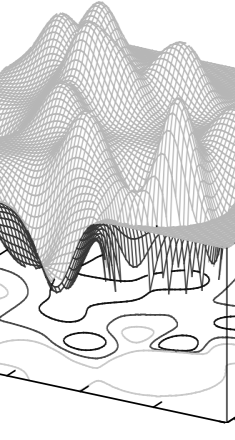
\includegraphics[height=7cm]{classPicture2-bw}
    }{\center

      \textbf{\fontsize{17}{20}\selectfont \course}

      ~

      %Lecture
      \topic\\

      \vspace{1cm}

      {\tiny~\emph{\keywords}~\\}

      \vspace{1cm}

      Marc Toussaint
      
      University of Stuttgart

      Summer 2019

      ~

    }
  }
}

\newcommand{\slide}[2]{
  \slidefont
  \incpage\begin{frame}
  \addcontentsline{toc}{section}{#1}
  \vfill
  {\headerfont #1} \vspace*{-2ex}
  \begin{itemize}\item[]~\\
    #2
  \end{itemize}
  \vfill
  \end{frame}
}

\newenvironment{slidecore}[1]{
  \slidefont\incpage
  \addcontentsline{toc}{section}{#1}
  \vfill
  {\headerfont #1} \vspace*{-2ex}
  \begin{itemize}\item[]~\\
}{
  \end{itemize}
  \vfill
}


\providecommand{\key}[1]{
  \addtocounter{mypage}{1}
% \immediate\write\keyfile{#1}
  \addtocontents{toc}{\hyperref[key:#1]{#1 (\arabic{mypage})}}
%  \phantomsection\label{key:#1}
%  \index{#1@{\hyperref[key:#1]{#1 (\arabic{mysec}:\arabic{mypage})}}|phantom}
  \addtocounter{mypage}{-1}
}

\providecommand{\course}{}

\providecommand{\subtopic}{}

\providecommand{\sublecture}[2]{
  \renewcommand{\subtopic}{#1}
  \slide{#1}{#2}
}

\providecommand{\story}[1]{
~

Motivation: {\tiny #1}\clearpage
}

\newenvironment{items}[1][9]{
\par\setlength{\unitlength}{1pt}\fontsize{#1}{#1}\linespread{1.2}\selectfont
\begin{list}{--}{\leftmargin4ex \rightmargin0ex \labelsep1ex \labelwidth2ex
\topsep0pt \parsep0ex \itemsep3pt}
}{
\end{list}
}

\providecommand{\slidesfoot}{
  \end{document}
}


  \slideshead
}

\providecommand{\exercises}{
  \newcommand{\exerciseshead}{
  \documentclass[10pt,fleqn]{article}
  \stdpackages

  \definecolor{bluecol}{rgb}{0,0,.5}
  \definecolor{greencol}{rgb}{0,.4,0}
  \definecolor{shadecolor}{gray}{0.9}
  \usepackage[
    %    pdftex%,
    %%    letterpaper,
    %    bookmarks,
    %    bookmarksnumbered,
    colorlinks,
    urlcolor=bluecol,
    citecolor=black,
    linkcolor=bluecol,
    %    pagecolor=bluecol,
    pdfborder={0 0 0},
    %pdfborderstyle={/S/U/W 1},
    %%    backref,     %link from bibliography back to sections
    %%    pagebackref, %link from bibliography back to pages
    %%    pdfstartview=FitH, %fitwidth instead of fit window
    pdfpagemode=UseNone, %UseOutlines, %bookmarks are displayed by acrobat
    pdftitle={\course},
    pdfauthor={Marc Toussaint},
    pdfkeywords={}
  ]{hyperref}
  \DeclareGraphicsExtensions{.pdf,.png,.jpg,.eps}

  \renewcommand{\r}{\varrho}
  \renewcommand{\l}{\lambda}
  \renewcommand{\L}{\Lambda}
  \renewcommand{\b}{\beta}
  \renewcommand{\d}{\delta}
  \renewcommand{\k}{\kappa}
  \renewcommand{\t}{\theta}
  \renewcommand{\O}{\Omega}
  \renewcommand{\o}{\omega}
  \renewcommand{\SS}{{\cal S}}
  \renewcommand{\=}{\!=\!}
  %\renewcommand{\boldsymbol}{}
  %\renewcommand{\Chapter}{\chapter}
  %\renewcommand{\Subsection}{\subsection}

  \renewcommand{\baselinestretch}{1.1}
  \geometry{a4paper,headsep=7mm,hdivide={15mm,*,15mm},vdivide={20mm,*,15mm}}

  \fancyhead[L]{\thetitle, \textit{Marc Toussaint}---\today}
  \fancyhead[R]{\thepage}
  \fancyhead[C]{}
  \fancyfoot{}
  \pagestyle{fancy}

  \parindent 0pt
  \parskip 0.5ex

  \newcommand{\codefont}{\helvetica{8}{1.2}{m}{n}}

  %auto-ignore
  \renewcommand{\a}{\alpha}
  \renewcommand{\b}{\beta}
  \renewcommand{\d}{\delta}
    \newcommand{\D}{\Delta}
    \newcommand{\e}{\epsilon}
    \newcommand{\g}{\gamma}
    \newcommand{\G}{\Gamma}
  \renewcommand{\l}{\lambda}
  \renewcommand{\L}{\Lambda}
    \newcommand{\m}{\mu}
    \newcommand{\n}{\nu}
    \newcommand{\N}{\nabla}
  \renewcommand{\k}{\kappa}
  \renewcommand{\o}{\omega}
  \renewcommand{\O}{\Omega}
    \newcommand{\p}{\phi}
    \newcommand{\ph}{\varphi}
  \renewcommand{\P}{\Phi}
  \renewcommand{\r}{\varrho}
    \newcommand{\s}{\sigma}
  \renewcommand{\S}{\Sigma}
  \renewcommand{\t}{\theta}
    \newcommand{\T}{\Theta}
  %\renewcommand{\v}{\vartheta}
    \newcommand{\x}{\xi}
    \newcommand{\X}{\Xi}
    \newcommand{\Y}{\Upsilon}
    \newcommand{\z}{\zeta}

  \renewcommand{\AA}{{\cal A}}
    \newcommand{\BB}{{\cal B}}
    \newcommand{\CC}{{\cal C}}
    \newcommand{\cc}{{\cal c}}
    \newcommand{\DD}{{\cal D}}
    \newcommand{\EE}{{\cal E}}
    \newcommand{\FF}{{\cal F}}
    \newcommand{\GG}{{\cal G}}
    \newcommand{\HH}{{\cal H}}
    \newcommand{\II}{{\cal I}}
    \newcommand{\KK}{{\cal K}}
    \newcommand{\LL}{{\cal L}}
    \newcommand{\MM}{{\cal M}}
    \newcommand{\NN}{{\cal N}}
    \newcommand{\oNN}{\overline\NN}
    \newcommand{\OO}{{\cal O}}
    \newcommand{\PP}{{\cal P}}
    \newcommand{\QQ}{{\cal Q}}
    \newcommand{\RR}{{\cal R}}
  \renewcommand{\SS}{{\cal S}}
    \newcommand{\TT}{{\cal T}}
    \newcommand{\uu}{{\cal u}}
    \newcommand{\UU}{{\cal U}}
    \newcommand{\VV}{{\cal V}}
    \newcommand{\XX}{{\cal X}}
    \newcommand{\xx}{\mathcal{x}}
    \newcommand{\YY}{{\cal Y}}
    \newcommand{\SOSO}{{\cal SO}}
    \newcommand{\GLGL}{{\cal GL}}

    \newcommand{\Ee}{{\rm E}}

  \newcommand{\NNN}{{\mathbb{N}}}
  \newcommand{\III}{{\mathbb{I}}}
  \newcommand{\ZZZ}{{\mathbb{Z}}}
  %\newcommand{\RRR}{{\mathrm{I\!R}}}
  \newcommand{\RRR}{{\mathbb{R}}}
  \newcommand{\SSS}{{\mathbb{S}}}
  \newcommand{\CCC}{{\mathbb{C}}}
  \newcommand{\DDD}{{\mathbb{D}}}
  \newcommand{\one}{{{\bf 1}}}
  \newcommand{\eee}{\text{e}}

  \newcommand{\NNNN}{{\overline{\cal N}}}

  \renewcommand{\[}{\Big[}
  \renewcommand{\]}{\Big]}
  \renewcommand{\(}{\Big(}
  \renewcommand{\)}{\Big)}
  \renewcommand{\|}{\,|\,}
  \renewcommand{\;}{\,;\,}
  \renewcommand{\=}{\!=\!}
    \newcommand{\<}{\left\langle}
  \renewcommand{\>}{\right\rangle}

  \newcommand{\na}[1][]{{\nabla_{\!\!#1}}}
  \newcommand{\he}[1][]{{\nabla_{\!\!#1}^2}}
  \newcommand{\Prob}{{\rm Prob}}
  \newcommand{\Dir}{{\rm Dir}}
  \newcommand{\Beta}{{\rm Beta}}
  \newcommand{\Bern}{{\rm Bern}}
  \newcommand{\Bin}{{\rm Bin}}
  \newcommand{\Mult}{{\rm Mult}}
  \newcommand{\Aut}{{\rm Aut}}
  \newcommand{\cor}{{\rm cor}}
  \newcommand{\corr}{{\rm corr}}
  \newcommand{\sd}{{\rm sd}}
  \newcommand{\tr}{{\rm tr}}
  \newcommand{\Tr}{{\rm Tr}}
  \newcommand{\rank}{{\rm rank}}
  \newcommand{\diag}{{\rm diag}}
  \newcommand{\dom}{{\rm dom}}
  \newcommand{\id}{{\rm id}}
  \newcommand{\Id}{{\rm\bf I}}
  \newcommand{\Gl}{{\rm Gl}}
  \renewcommand{\th}{\ensuremath{{}^\text{th}} }
  \newcommand{\lag}{\mathcal{L}}
  \newcommand{\inn}{\rfloor}
  \newcommand{\lie}{\pounds}
  \newcommand{\longto}{\longrightarrow}
  \newcommand{\speer}{\parbox{0.4ex}{\raisebox{0.8ex}{$\nearrow$}}}
  \renewcommand{\dag}{ {}^\dagger }
  \newcommand{\blbox}{\rule{1ex}{1ex}}
  \newcommand{\Ji}{J^\sharp}
  \newcommand{\h}{{}^\star}
  \newcommand{\w}{\wedge}
  \newcommand{\too}{\longrightarrow}
  \newcommand{\oot}{\longleftarrow}
  \newcommand{\To}{\Rightarrow}
  \newcommand{\oT}{\Leftarrow}
  \newcommand{\oTo}{\Leftrightarrow}
  \renewcommand{\iff}{~\Longleftrightarrow~}
  \newcommand{\Too}{\;\Longrightarrow\;}
  \newcommand{\oto}{\leftrightarrow}
  \newcommand{\ot}{\leftarrow}
  \newcommand{\ootoo}{\longleftrightarrow}
  \newcommand{\ow}{\stackrel{\circ}\wedge}
  \newcommand{\defeq}{\stackrel{\hspace{0.2ex}{}_\Delta}=}
%  \newcommand{\defeq}{{\overstack\Delta =}}
  \newcommand{\feed}{\nonumber \\}
  \newcommand{\comma}{~,\quad}
  \newcommand{\period}{~.\quad}
  \newcommand{\del}{\partial}
%  \newcommand{\quabla}{\Delta}
  \newcommand{\point}{$\bullet~~$}
  \newcommand{\doubletilde}{ ~ \raisebox{0.3ex}{$\widetilde {}$} \raisebox{0.6ex}{$\widetilde {}$} \!\! }
  \newcommand{\topcirc}{\parbox{0ex}{~\raisebox{2.5ex}{${}^\circ$}}}
  \newcommand{\topdot} {\parbox{0ex}{~\raisebox{2.5ex}{$\cdot$}}}
  \newcommand{\topddot} {\parbox{0ex}{~\raisebox{1.3ex}{$\ddot{~}$}}}
  \newcommand{\sym}{\topcirc}
  \newcommand{\tsum}{\textstyle\sum}
  \newcommand{\st}{\quad\text{s.t.}\quad}

  \newcommand{\half}{\ensuremath{\frac{1}{2}}}
  \newcommand{\third}{\ensuremath{\frac{1}{3}}}
  \newcommand{\fourth}{\ensuremath{\frac{1}{4}}}

  \newcommand{\ubar}{\underline}
  %\renewcommand{\vec}{\underline}
  \renewcommand{\vec}{\boldsymbol}
  %\renewcommand{\_}{\underset}
  %\renewcommand{\^}{\overset}
  %\renewcommand{\*}{{\rm\raisebox{-.6ex}{\text{*}}{}}}
  \renewcommand{\*}{\text{\footnotesize\raisebox{-.4ex}{*}{}}}

  \newcommand{\gto}{{\raisebox{.5ex}{${}_\rightarrow$}}}
  \newcommand{\gfrom}{{\raisebox{.5ex}{${}_\leftarrow$}}}
  \newcommand{\gnto}{{\raisebox{.5ex}{${}_\nrightarrow$}}}
  \newcommand{\gnfrom}{{\raisebox{.5ex}{${}_\nleftarrow$}}}

  %\newcommand{\RND}{{\SS}}
  %\newcommand{\IF}{\text{if }}
  %\newcommand{\AND}{\textsc{and }}
  %\newcommand{\OR}{\textsc{or }}
  %\newcommand{\XOR}{\textsc{xor }}
  %\newcommand{\NOT}{\textsc{not }}

  %\newcommand{\argmax}[1]{{\rm arg}\!\max_{#1}}
  %\newcommand{\argmin}[1]{{\rm arg}\!\min_{#1}}
  \DeclareMathOperator*{\argmax}{argmax}
  \DeclareMathOperator*{\argmin}{argmin}
  \DeclareMathOperator{\sign}{sign}
  \DeclareMathOperator{\acos}{acos}
  \DeclareMathOperator{\unifies}{unifies}
  \DeclareMathOperator{\Span}{span}
  \newcommand{\ortho}{\perp}
  %\newcommand{\argmax}[1]{\underset{~#1}{\text{argmax}}\;}
  %\newcommand{\argmin}[1]{\underset{~#1}{\text{argmin}}\;}
  \newcommand{\ee}[1]{\ensuremath{\cdot10^{#1}}}
  \newcommand{\sub}[1]{\ensuremath{_{\text{#1}}}}
  \newcommand{\up}[1]{\ensuremath{^{\text{#1}}}}
  \newcommand{\kld}[3][{}]{D_{#1}\big(#2\,\big|\!\big|\,#3\big)}
  %\newcommand{\kld}[2]{D\big(#1:#2\big)}
  \newcommand{\sprod}[2]{\big<#1\,,\,#2\big>}
  \newcommand{\End}{\text{End}}
  \newcommand{\txt}[1]{\quad\text{#1}\quad}
  \newcommand{\Over}[2]{\genfrac{}{}{0pt}{0}{#1}{#2}}
  %\newcommand{\mat}[1]{{\bf #1}}
  \newcommand{\arr}[2]{\hspace*{-.5ex}\begin{array}{#1}#2\end{array}\hspace*{-.5ex}}
  \newcommand{\mat}[3][.9]{
    \renewcommand{\arraystretch}{#1}{\scriptscriptstyle{\left(
      \hspace*{-1ex}\begin{array}{#2}#3\end{array}\hspace*{-1ex}
    \right)}}\renewcommand{\arraystretch}{1.2}
  }
  \newcommand{\Mat}[3][.9]{
    \renewcommand{\arraystretch}{#1}{\scriptscriptstyle{\left[
      \hspace*{-1ex}\begin{array}{#2}#3\end{array}\hspace*{-1ex}
    \right]}}\renewcommand{\arraystretch}{1.2}
  }
  \newcommand{\case}[2][ll]{\left\{\arr{#1}{#2}\right.}
  \newcommand{\seq}[1]{\textsf{\<#1\>}}
  \newcommand{\seqq}[1]{\textsf{#1}}
  \newcommand{\floor}[1]{\lfloor#1\rfloor}
  \newcommand{\Exp}[2][]{\text{E}_{#1}\{#2\}}
  \newcommand{\Var}[2][]{\text{Var}_{#1}\{#2\}}
  \newcommand{\cov}[2][]{\text{cov}_{#1}\{#2\}}

  %\newcommand{\Exp}[2]{\left\langle{#2}\right\rangle_{#1}}
  \newcommand{\ex}{\setminus}

  \providecommand{\href}[2]{{\color{blue}USE PDFLATEX!}}
  \providecommand{\url}[2]{\href{#1}{{\color{blue}#2}}}
%  \newcommand{\link}[1]{\href{{\protect #1}}{\texttt{\protect #1}}}
  \newcommand{\anchor}[2]{\begin{picture}(0,0)\put(#1){#2}\end{picture}}
  \newcommand{\pagebox}{\begin{picture}(0,0)\put(-3,-23){
    \textcolor[rgb]{.5,1,.5}{\framebox[\textwidth]{\rule[-\textheight]{0pt}{0pt}}}}
    \end{picture}}

  \newcommand{\hide}[1]{
    \begin{list}{}{\leftmargin0ex \rightmargin0ex \topsep0ex \parsep0ex}
       \helvetica{5}{1}{m}{n}
       \renewcommand{\section}{\par SECTION: }
       \renewcommand{\subsection}{\par SUBSECTION: }
       \item[$~~\blacktriangleright$]
       #1%$\blacktriangleleft~~$
       \message{^^JHIDE--Warning!^^J}
    \end{list}
  }
  %\newcommand{\hide}[1]{{\tt[hide:~}{\footnotesize\sf #1}{\tt]}\message{^^JHIDE--Warning!^^J}}
  \newcommand{\Hide}{\renewcommand{\hide}[1]{\message{^^JHIDE--Warning (hidden)!^^J}}}
  \newcommand{\HIDE}{\renewcommand{\hide}[1]{}}
  \newcommand{\fullhide}[1]{\message{^^JHIDE--Warning (hidden)!^^J}}
  \newcommand{\todo}[1]{{\tt[TODO: #1]}\message{^^JTODO--Warning: #1^^J}}
  \newcommand{\Todo}{\renewcommand{\todo}[1]{\message{^^JTODO--Warning (hidden)!^^J}}}
  %\renewcommand{\title}[1]{\renewcommand{\thetitle}{#1}}
  \newcommand{\myauthor}[1]{\author{#1}\newcommand{\theauthor}{#1}}%\@author}
  \newcommand{\mytitle}[1]{\title{#1}\newcommand{\thetitle}{#1}}%\@title}
  \newcommand{\header}{\begin{document}\mytitle\cleardefs}
  \newcommand{\contents}{{\tableofcontents}\renewcommand{\contents}{}}
  \newcommand{\footer}{\small\bibliography{marc,bibs}\end{document}}
  \newcommand{\widepaper}{\usepackage{geometry}\geometry{a4paper,hdivide={25mm,*,25mm},vdivide={25mm,*,25mm}}}
  \newcommand{\moviex}[2]{\movie[externalviewer]{#1}{#2}} %\pdflatex\usepackage{multimedia}
  \newcommand{\rbox}[1]{\fboxrule2mm\fcolorbox[rgb]{1,.85,.85}{1,.85,.85}{#1}}
  \newcommand{\mpage}[2]{{\begin{minipage}{#1\columnwidth}#2\end{minipage}}}
  \newcommand{\redbox}[2]{\fboxrule1mm\fcolorbox[rgb]{1,.7,.7}{1,.7,.7}{\begin{minipage}{#1\columnwidth}\center#2\end{minipage}}}
  \newcommand{\onecol}[2]{
    \begin{minipage}[c]{#1\columnwidth}#2\end{minipage}}
  \newcommand{\twocol}[5][0]{
    \begin{minipage}[c]{#2\columnwidth}#4\end{minipage}\hspace*{#1\columnwidth}%
    \begin{minipage}[c]{#3\columnwidth}#5\end{minipage}}
  \newcommand{\threecol}[7][0]{%
    \begin{minipage}[c]{#2\columnwidth}#5\end{minipage}\hspace*{#1\columnwidth}%
    \begin{minipage}[c]{#3\columnwidth}#6\end{minipage}\hspace*{#1\columnwidth}%
    \begin{minipage}[c]{#4\columnwidth}#7\end{minipage}}
  \newcommand{\threecoltext}[7][c]{
    \begin{minipage}[#1]{#2\textwidth}#5\end{minipage}%
    \begin{minipage}[#1]{#3\textwidth}#6\end{minipage}%
    \begin{minipage}[#1]{#4\textwidth}#7\end{minipage}}
  \newcommand{\threecoltop}[7][0]{%
   \begin{minipage}[t]{#2\columnwidth}#5\end{minipage}\hspace*{#1\columnwidth}%
   \begin{minipage}[t]{#3\columnwidth}#6\end{minipage}\hspace*{#1\columnwidth}%
   \begin{minipage}[t]{#4\columnwidth}#7\end{minipage}}
  \newcommand{\fourcol}[9][0]{%
   \begin{minipage}[c]{#2\columnwidth}#6\end{minipage}\hspace*{#1\columnwidth}%
   \begin{minipage}[c]{#3\columnwidth}#7\end{minipage}\hspace*{#1\columnwidth}%
   \begin{minipage}[c]{#4\columnwidth}#8\end{minipage}\hspace*{#1\columnwidth}%
   \begin{minipage}[c]{#5\columnwidth}#9\end{minipage}}
  \newcommand{\helvetica}[4]{\setlength{\unitlength}{1pt}\fontsize{#1}{#1}\linespread{#2}\usefont{OT1}{phv}{#3}{#4}}
  \newcommand{\helve}[1]{\helvetica{#1}{1.5}{m}{n}}
  \newcommand{\german}{\usepackage[german]{babel}\usepackage[utf8]{inputenc}}

\newcommand{\norm}[1]{|\!|#1|\!|}
\newcommand{\expr}[1]{[\hspace{-.2ex}[#1]\hspace{-.2ex}]}

\newcommand{\Jwi}{J^\sharp_W}
\newcommand{\THi}{T^\sharp_H}
\newcommand{\Jci}{J^\natural_C}
\newcommand{\hJi}{{\bar J}^\sharp}
\renewcommand{\|}{\,|\,}
\renewcommand{\=}{\!=\!}
\newcommand{\myminus}{{\hspace*{-.0pt}\text{\rm -}\hspace*{-.5pt}}}
\newcommand{\myplus}{{\hspace*{-.0pt}\text{\rm +}\hspace*{-.5pt}}}
\newcommand{\1}{{\myminus1}}
\newcommand{\2}{{\myminus2}}
\newcommand{\3}{{\myminus3}}
\newcommand{\mT}{{\text{\rm -}\hspace*{-1pt}\top}}
\newcommand{\po}{{\myplus1}}
\newcommand{\pt}{{\myplus2}}
%\renewcommand{\-}{\myminus}
%\newcommand{\+}{\myplus}
\renewcommand{\T}{{\!\top\!}}
\newcommand{\xT}{{\underline x}}
\newcommand{\uT}{{\underline u}}
\newcommand{\zT}{{\underline z}}
\newcommand{\Sum}{\textstyle\sum}
\newcommand{\Int}{\textstyle\int}
\newcommand{\Prod}{\textstyle\prod}


\newenvironment{centy}{
\vspace{15mm}
\large
\hspace*{5mm}
\begin{minipage}{8cm}\it\color{blue}
}{
\end{minipage}
}

\newcommand{\old}{{\text{old}}}
\newcommand{\new}{{\text{new}}}
\newcommand{\MAP}{{\text{MAP}}}
\newcommand{\ML}{{\text{ML}}}

\newcommand{\redArrow}{\quad\anchor{0,-1}{\includegraphics[scale=.5]{figs/redArrow}}}
\newcommand{\pub}[1]{{\color{green}\helvetica{8}{1.3}{m}{n}#1\\}}
\DeclareMathOperator{\opKL}{KL}
\newcommand{\KL}[2]{\opKL\big(#1\,\big|\!\big|\,#2\big)} %\left(#1 |\!| #2\right)}

\renewcommand{\show}[2][.8]{\centerline{\includegraphics[width=#1\columnwidth]{#2}}}
\newcommand{\showh}[2][.8]{\includegraphics[width=#1\columnwidth]{#2}}
\newcommand{\shows}[2][.8]{\centerline{\includegraphics[scale=#1]{#2}}}
\newcommand{\showhs}[2][.8]{\includegraphics[scale=#1]{#2}}
\newcommand{\mov}[2]{\movie[externalviewer]{{\color{blue}\small #1}}{movies/#2}}
\newcommand{\movex}[2]{\movie[externalviewer]{#1}{#2}} %\pdflatex\usepackage{multimedia}
%\newcommand{\movgb}[1]{\hfill\movie[externalviewer]{\small[movie]}{/home/mtoussai/movies/10-goalDirectedBehavior/#1}}
\newcommand{\movh}[3][loop]{
\movie[#1]{\showh[#2]{movies/#3.png}}{movies/#3.avi}%
\movie[externalviewer]{$\circ$}{movies/#3.avi}
}
\newcommand{\movc}[3][loop]{\centerline{\movh[#1]{#2}{#3}}}
\newcommand{\cen}[1]{\centerline{#1}}

\newcommand{\citing}[1]{
{\color{citcol}\tiny#1\par}
}

\newcommand{\cit}[3]{
\par\smallskip
{\color{greencol}\tiny #1: \emph{#2}. #3 \par}
}

\newcommand{\citurl}[4]{
\par\smallskip
{\color{greencol}\tiny #1: \protect{\href{#4}{\color{blue}{#2.}}} #3 \par}
}

\newcommand{\cito}[3]{
\par\smallskip
{\color{bluecol}\tiny #1: \emph{#2}. #3 \par}
}

\newcommand{\redoMacrosInProof}{
  \renewcommand{\d}{\delta}
%  \renewcommand{\|}{\,|\,}
  \renewcommand{\=}{\!=\!}
}

%% \makeatletter
%% \newenvironment{code}{%
%%   \begin{lrbox}{\@tempboxa}\begin{minipage}{1\columnwidth}\codefont
%% }{
%%   \end{minipage}\end{lrbox}%
%%   \colorbox[rgb]{.95,.95,.95}{\usebox{\@tempboxa}}
%% }\makeatother

\newenvironment{code}{%
\codefont
\begin{shaded}
}{
\end{shaded}
}

%\newcommand{\refeq}[1]{(\ref{#1})}

\usepackage{algorithm}
\usepackage{algpseudocode}
\algrenewcommand{\algorithmicrequire}{\textbf{Input:~~}}
\algrenewcommand{\algorithmicensure}{\textbf{Output:}}
\algrenewcommand{\algorithmiccomment}[1]{\qquad\hfill~\hspace*{-5ex}\textit{// #1}}
\algrenewcommand{\alglinenumber}[1]{\helvetica{6}{1.3}{m}{n}#1:}

\newenvironment{algo}[1][8]{
\quad\begin{minipage}{.8\columnwidth}\helvetica{#1}{1.3}{m}{n}
\medskip\hrule\medskip
\begin{algorithmic}[1]
}{
\end{algorithmic}
\medskip\hrule\medskip
\end{minipage}
}

\usepackage{etoolbox}

%%%%%%%%%%%%%%%%%%%%%%%%%%%%%%%%%%%%%%%%%%%%%%%%%%%%%%%%%%%%%%%%%%%%%%%%%%%%%%%%

\usepackage{multirow}
\usepackage{colortbl}
%\setlength{\jot}{0pt}
%\setlength{\mathindent}{1ex}
\usepackage{empheq}

%%%%%%%%%%%%%%%%%%%%%%%%%%%%%%%%%%%%%%%%%%%%%%%%%%%%%%%%%%%%%%%%%%%%%%%%%%%%%%%

\newcommand{\mypause}{\pause}
%\newcommand{\dom}{{\text{dom}}}
\newcommand{\defi}[1]{\textbf{#1}}
\newcommand{\red}[1]{\emph{\color{red}#1}}
%\newcommand{\ul}{\underline}
\newcommand{\pos}{{\textsf{pos}}}
\newcommand{\eff}{{\textsf{eff}}}
\newcommand{\rot}{{\textsf{rot}}}
\newcommand{\veC}{{\textsf{vec}}}
\newcommand{\quat}{{\textsf{quat}}}
\newcommand{\col}{{\textsf{col}}}
\newcommand{\de}[2]{\frac{\partial #1}{\partial #2}}
\newcommand{\target}{{\text{target}}}
\newcommand{\near}{{\text{near}}}
\newcommand{\qfree}{Q_{\text{free}}}
\renewcommand{\vec}{\boldsymbol}
\newcommand{\lft}{\text{left}}
\newcommand{\rgh}{\text{right}}
\DeclareMathOperator{\real}{real}
\newcommand{\prev}{{\text{prev}}}
\newcommand{\TR}[2]{T_{{#1}\shortrightarrow{#2}}}
\newcommand{\RO}[2]{R_{{#1}\shortrightarrow{#2}}}
\newcommand{\liter}{\helvetica{8}{1.1}{m}{n}\parskip 1ex}
\newcommand{\Fc}{\color{green}F}
\newcommand{\muc}{\color{blue}\mu}
\newcommand{\Astar}{A$^*$}

%for optimization course:
\newcommand{\adec}{\r_\a^-}
\newcommand{\ainc}{\r_\a^+}
\newcommand{\ldec}{\r_\l^-}
\newcommand{\linc}{\r_\l^+}
\newcommand{\minc}{\r_\m^+}
\newcommand{\mdec}{\r_\m^-}
\newcommand{\lsstop}{\r_{\text{ls}}}


\definecolor{boxcol}{rgb}{.85,.9,.92}
\newcommand{\eqbox}[1]{\centerline{\fboxrule0mm\fcolorbox{boxcol}{boxcol}{#1}}}
\newcommand{\movgb}[1]{\hfill\movie[externalviewer]{\small[movie]}{/home/mtoussai/movies/10-goalDirectedBehavior/#1}}
\newcommand{\demo}[1]{{{\color{blue}[\small #1]}}}

\graphicspath{{../pics-robotics/}{../pics-ML/}{../pics-all/}{../pics-all2/}{../pics-Optim/}}
\DeclareGraphicsExtensions{.pdf,.png,.jpg}

%\usepackage{pdfpages}
%\setbeamercolor{background canvas}{bg=}

\newcommand{\SUM}{\texttt{sum}}
\usepackage{float}

%% prevent pagebreaks before environment
\makeatletter
\newcommand{\NewParNoBreak}[1][\parskip]{\par\vspace*{-\parskip}\vspace*{#1}\nobreak\@afterheading}
\makeatother

%\newcommand{\idx}[2]{\label{IKgn}}

%%%%%%%%%%%%%%%%%%%%%%%%%%%%%%%%%%%%%%%%%%%%%%%%%%%%%%%%%%%%%%%%%%%%%%%%%%%%%%%%



%% \newwrite\tempfile
%% \immediate\openout\tempfile=z.keys.tex

%% \renewcommand{\key}[1]{
%% %%   \addtocounter{mypage}{1}
%% \makeatletter
%% \immediate\write\tempfile{\symbol{`\\}}
%% \makeatother
%%   \immediate\write\tempfile{hyperref[key:#1]{#1(\arabic{mypage})}}
%% %%  % \phantomsection\label{key:#1}
%% %%   %\index{#1@{\hyperref[key:#1]{#1 (\arabic{mysec}:\arabic{mypage})}}|phantom}
%% %%   \addtocounter{mypage}{-1}
%% }


  \DefineShortVerb{\@}

  \newcounter{solutions}
  \setcounter{solutions}{1}
  \newenvironment{solution}{
    \small
    \begin{shaded}
  }{
    \end{shaded}
  }
  
  \renewcommand{\hat}{\widehat}
  \newcommand{\bbg}{{\bar{\bar g}}}
  \graphicspath{{pics/}{../shared/pics/}}

  \renewcommand{\labelenumi}{{\alph{enumi})}}

  %%%%%%%%%%%%%%%%%%%%%%%%%%%%%%%%%%%%%%%%%%%%%%%%%%%%%%%%%%%%%%%%%%%%%%%%%%%%%%%%


  \mytitle{\course\\Exercise \exnum}
  \myauthor{Marc Toussaint\\ TAs: Janik Hager, Philipp Kratzer\\\small\addressUSTT}
  
  
  \begin{document}
  \onecolumn
  \maketitle
}

\newcommand{\exsection}[1]{\section{#1}}

\newcommand{\exerfoot}{
  \end{document}
}

\newenvironment{items}[1][9]{
  \par\setlength{\unitlength}{1pt}\fontsize{#1}{#1}\linespread{1.2}\selectfont
  \begin{list}{--}{\leftmargin4ex \rightmargin0ex \labelsep1ex \labelwidth2ex
      \topsep0pt \parsep0ex \itemsep3pt}
}{
  \end{list}
}

  \exerciseshead
}

\providecommand{\script}{
  \newcommand{\scripthead}{
  \documentclass[9pt,twoside]{article}
  \stdpackages

  \usepackage{palatino}
  \usepackage[envcountsect]{beamerarticle}
  \usepackage{makeidx}
  \makeindex

  \definecolor{bluecol}{rgb}{0,0,.5}
  \definecolor{greencol}{rgb}{0,.4,0}
  \definecolor{shadecolor}{gray}{0.9}
  \usepackage[
    %    pdftex%,
    %%    letterpaper,
    %bookmarks,
    bookmarksnumbered,
    colorlinks,
    urlcolor=bluecol,
    citecolor=black,
    linkcolor=bluecol,
    %    pagecolor=bluecol,
    pdfborder={0 0 0},
    %pdfborderstyle={/S/U/W 1},
    %%    backref,     %link from bibliography back to sections
    %%    pagebackref, %link from bibliography back to pages
    %%    pdfstartview=FitH, %fitwidth instead of fit window
    pdfpagemode=UseOutlines, %bookmarks are displayed by acrobat
    pdftitle={\course},
    pdfauthor={Marc Toussaint},
    pdfkeywords={}
  ]{hyperref}
  \DeclareGraphicsExtensions{.pdf,.png,.jpg,.eps}

  \usepackage{multimedia}
  %\setbeamercolor{background canvas}{bg=}

  \renewcommand{\r}{\varrho}
  \renewcommand{\l}{\lambda}
  \renewcommand{\L}{\Lambda}
  \renewcommand{\b}{\beta}
  \renewcommand{\d}{\delta}
  \renewcommand{\k}{\kappa}
  \renewcommand{\t}{\theta}
  \renewcommand{\O}{\Omega}
  \renewcommand{\o}{\omega}
  \renewcommand{\SS}{{\cal S}}
  \renewcommand{\=}{\!=\!}
  %\renewcommand{\boldsymbol}{}
  %\renewcommand{\Chapter}{\chapter}
  %\renewcommand{\Subsection}{\subsection}

  \renewcommand{\baselinestretch}{1.0}
  \geometry{a5paper,headsep=6mm,hdivide={10mm,*,10mm},vdivide={13mm,*,7mm}}

  \fancyhead[OL,ER]{\course, \textit{Marc Toussaint}}
  \fancyhead[OR,EL]{\thepage}
  \fancyhead[C]{}
  \fancyfoot{}
  \pagestyle{fancy}

%  \setcounter{tocdepth}{3}
  \setcounter{tocdepth}{2}

   \columnsep 6ex
  %  \renewcommand{\familydefault}{\sfdefault}
  \newcommand{\headerfont}{\large}%helvetica{12}{1}{b}{n}}
  \newcommand{\slidefont} {}%\helvetica{9}{1.3}{m}{n}}
  \newcommand{\storyfont} {}
  %  \renewcommand{\small}   {\helvetica{8}{1.2}{m}{n}}
  \renewcommand{\tiny}    {\footnotesize}%helvetica{7}{1.1}{m}{n}}
  \newcommand{\codefont}{\fontsize{6}{6}\selectfont}%helvetica{8}{1.2}{m}{n}}

  %auto-ignore
  \renewcommand{\a}{\alpha}
  \renewcommand{\b}{\beta}
  \renewcommand{\d}{\delta}
    \newcommand{\D}{\Delta}
    \newcommand{\e}{\epsilon}
    \newcommand{\g}{\gamma}
    \newcommand{\G}{\Gamma}
  \renewcommand{\l}{\lambda}
  \renewcommand{\L}{\Lambda}
    \newcommand{\m}{\mu}
    \newcommand{\n}{\nu}
    \newcommand{\N}{\nabla}
  \renewcommand{\k}{\kappa}
  \renewcommand{\o}{\omega}
  \renewcommand{\O}{\Omega}
    \newcommand{\p}{\phi}
    \newcommand{\ph}{\varphi}
  \renewcommand{\P}{\Phi}
  \renewcommand{\r}{\varrho}
    \newcommand{\s}{\sigma}
  \renewcommand{\S}{\Sigma}
  \renewcommand{\t}{\theta}
    \newcommand{\T}{\Theta}
  %\renewcommand{\v}{\vartheta}
    \newcommand{\x}{\xi}
    \newcommand{\X}{\Xi}
    \newcommand{\Y}{\Upsilon}
    \newcommand{\z}{\zeta}

  \renewcommand{\AA}{{\cal A}}
    \newcommand{\BB}{{\cal B}}
    \newcommand{\CC}{{\cal C}}
    \newcommand{\cc}{{\cal c}}
    \newcommand{\DD}{{\cal D}}
    \newcommand{\EE}{{\cal E}}
    \newcommand{\FF}{{\cal F}}
    \newcommand{\GG}{{\cal G}}
    \newcommand{\HH}{{\cal H}}
    \newcommand{\II}{{\cal I}}
    \newcommand{\KK}{{\cal K}}
    \newcommand{\LL}{{\cal L}}
    \newcommand{\MM}{{\cal M}}
    \newcommand{\NN}{{\cal N}}
    \newcommand{\oNN}{\overline\NN}
    \newcommand{\OO}{{\cal O}}
    \newcommand{\PP}{{\cal P}}
    \newcommand{\QQ}{{\cal Q}}
    \newcommand{\RR}{{\cal R}}
  \renewcommand{\SS}{{\cal S}}
    \newcommand{\TT}{{\cal T}}
    \newcommand{\uu}{{\cal u}}
    \newcommand{\UU}{{\cal U}}
    \newcommand{\VV}{{\cal V}}
    \newcommand{\XX}{{\cal X}}
    \newcommand{\xx}{\mathcal{x}}
    \newcommand{\YY}{{\cal Y}}
    \newcommand{\SOSO}{{\cal SO}}
    \newcommand{\GLGL}{{\cal GL}}

    \newcommand{\Ee}{{\rm E}}

  \newcommand{\NNN}{{\mathbb{N}}}
  \newcommand{\III}{{\mathbb{I}}}
  \newcommand{\ZZZ}{{\mathbb{Z}}}
  %\newcommand{\RRR}{{\mathrm{I\!R}}}
  \newcommand{\RRR}{{\mathbb{R}}}
  \newcommand{\SSS}{{\mathbb{S}}}
  \newcommand{\CCC}{{\mathbb{C}}}
  \newcommand{\DDD}{{\mathbb{D}}}
  \newcommand{\one}{{{\bf 1}}}
  \newcommand{\eee}{\text{e}}

  \newcommand{\NNNN}{{\overline{\cal N}}}

  \renewcommand{\[}{\Big[}
  \renewcommand{\]}{\Big]}
  \renewcommand{\(}{\Big(}
  \renewcommand{\)}{\Big)}
  \renewcommand{\|}{\,|\,}
  \renewcommand{\;}{\,;\,}
  \renewcommand{\=}{\!=\!}
    \newcommand{\<}{\left\langle}
  \renewcommand{\>}{\right\rangle}

  \newcommand{\na}[1][]{{\nabla_{\!\!#1}}}
  \newcommand{\he}[1][]{{\nabla_{\!\!#1}^2}}
  \newcommand{\Prob}{{\rm Prob}}
  \newcommand{\Dir}{{\rm Dir}}
  \newcommand{\Beta}{{\rm Beta}}
  \newcommand{\Bern}{{\rm Bern}}
  \newcommand{\Bin}{{\rm Bin}}
  \newcommand{\Mult}{{\rm Mult}}
  \newcommand{\Aut}{{\rm Aut}}
  \newcommand{\cor}{{\rm cor}}
  \newcommand{\corr}{{\rm corr}}
  \newcommand{\sd}{{\rm sd}}
  \newcommand{\tr}{{\rm tr}}
  \newcommand{\Tr}{{\rm Tr}}
  \newcommand{\rank}{{\rm rank}}
  \newcommand{\diag}{{\rm diag}}
  \newcommand{\dom}{{\rm dom}}
  \newcommand{\id}{{\rm id}}
  \newcommand{\Id}{{\rm\bf I}}
  \newcommand{\Gl}{{\rm Gl}}
  \renewcommand{\th}{\ensuremath{{}^\text{th}} }
  \newcommand{\lag}{\mathcal{L}}
  \newcommand{\inn}{\rfloor}
  \newcommand{\lie}{\pounds}
  \newcommand{\longto}{\longrightarrow}
  \newcommand{\speer}{\parbox{0.4ex}{\raisebox{0.8ex}{$\nearrow$}}}
  \renewcommand{\dag}{ {}^\dagger }
  \newcommand{\blbox}{\rule{1ex}{1ex}}
  \newcommand{\Ji}{J^\sharp}
  \newcommand{\h}{{}^\star}
  \newcommand{\w}{\wedge}
  \newcommand{\too}{\longrightarrow}
  \newcommand{\oot}{\longleftarrow}
  \newcommand{\To}{\Rightarrow}
  \newcommand{\oT}{\Leftarrow}
  \newcommand{\oTo}{\Leftrightarrow}
  \renewcommand{\iff}{~\Longleftrightarrow~}
  \newcommand{\Too}{\;\Longrightarrow\;}
  \newcommand{\oto}{\leftrightarrow}
  \newcommand{\ot}{\leftarrow}
  \newcommand{\ootoo}{\longleftrightarrow}
  \newcommand{\ow}{\stackrel{\circ}\wedge}
  \newcommand{\defeq}{\stackrel{\hspace{0.2ex}{}_\Delta}=}
%  \newcommand{\defeq}{{\overstack\Delta =}}
  \newcommand{\feed}{\nonumber \\}
  \newcommand{\comma}{~,\quad}
  \newcommand{\period}{~.\quad}
  \newcommand{\del}{\partial}
%  \newcommand{\quabla}{\Delta}
  \newcommand{\point}{$\bullet~~$}
  \newcommand{\doubletilde}{ ~ \raisebox{0.3ex}{$\widetilde {}$} \raisebox{0.6ex}{$\widetilde {}$} \!\! }
  \newcommand{\topcirc}{\parbox{0ex}{~\raisebox{2.5ex}{${}^\circ$}}}
  \newcommand{\topdot} {\parbox{0ex}{~\raisebox{2.5ex}{$\cdot$}}}
  \newcommand{\topddot} {\parbox{0ex}{~\raisebox{1.3ex}{$\ddot{~}$}}}
  \newcommand{\sym}{\topcirc}
  \newcommand{\tsum}{\textstyle\sum}
  \newcommand{\st}{\quad\text{s.t.}\quad}

  \newcommand{\half}{\ensuremath{\frac{1}{2}}}
  \newcommand{\third}{\ensuremath{\frac{1}{3}}}
  \newcommand{\fourth}{\ensuremath{\frac{1}{4}}}

  \newcommand{\ubar}{\underline}
  %\renewcommand{\vec}{\underline}
  \renewcommand{\vec}{\boldsymbol}
  %\renewcommand{\_}{\underset}
  %\renewcommand{\^}{\overset}
  %\renewcommand{\*}{{\rm\raisebox{-.6ex}{\text{*}}{}}}
  \renewcommand{\*}{\text{\footnotesize\raisebox{-.4ex}{*}{}}}

  \newcommand{\gto}{{\raisebox{.5ex}{${}_\rightarrow$}}}
  \newcommand{\gfrom}{{\raisebox{.5ex}{${}_\leftarrow$}}}
  \newcommand{\gnto}{{\raisebox{.5ex}{${}_\nrightarrow$}}}
  \newcommand{\gnfrom}{{\raisebox{.5ex}{${}_\nleftarrow$}}}

  %\newcommand{\RND}{{\SS}}
  %\newcommand{\IF}{\text{if }}
  %\newcommand{\AND}{\textsc{and }}
  %\newcommand{\OR}{\textsc{or }}
  %\newcommand{\XOR}{\textsc{xor }}
  %\newcommand{\NOT}{\textsc{not }}

  %\newcommand{\argmax}[1]{{\rm arg}\!\max_{#1}}
  %\newcommand{\argmin}[1]{{\rm arg}\!\min_{#1}}
  \DeclareMathOperator*{\argmax}{argmax}
  \DeclareMathOperator*{\argmin}{argmin}
  \DeclareMathOperator{\sign}{sign}
  \DeclareMathOperator{\acos}{acos}
  \DeclareMathOperator{\unifies}{unifies}
  \DeclareMathOperator{\Span}{span}
  \newcommand{\ortho}{\perp}
  %\newcommand{\argmax}[1]{\underset{~#1}{\text{argmax}}\;}
  %\newcommand{\argmin}[1]{\underset{~#1}{\text{argmin}}\;}
  \newcommand{\ee}[1]{\ensuremath{\cdot10^{#1}}}
  \newcommand{\sub}[1]{\ensuremath{_{\text{#1}}}}
  \newcommand{\up}[1]{\ensuremath{^{\text{#1}}}}
  \newcommand{\kld}[3][{}]{D_{#1}\big(#2\,\big|\!\big|\,#3\big)}
  %\newcommand{\kld}[2]{D\big(#1:#2\big)}
  \newcommand{\sprod}[2]{\big<#1\,,\,#2\big>}
  \newcommand{\End}{\text{End}}
  \newcommand{\txt}[1]{\quad\text{#1}\quad}
  \newcommand{\Over}[2]{\genfrac{}{}{0pt}{0}{#1}{#2}}
  %\newcommand{\mat}[1]{{\bf #1}}
  \newcommand{\arr}[2]{\hspace*{-.5ex}\begin{array}{#1}#2\end{array}\hspace*{-.5ex}}
  \newcommand{\mat}[3][.9]{
    \renewcommand{\arraystretch}{#1}{\scriptscriptstyle{\left(
      \hspace*{-1ex}\begin{array}{#2}#3\end{array}\hspace*{-1ex}
    \right)}}\renewcommand{\arraystretch}{1.2}
  }
  \newcommand{\Mat}[3][.9]{
    \renewcommand{\arraystretch}{#1}{\scriptscriptstyle{\left[
      \hspace*{-1ex}\begin{array}{#2}#3\end{array}\hspace*{-1ex}
    \right]}}\renewcommand{\arraystretch}{1.2}
  }
  \newcommand{\case}[2][ll]{\left\{\arr{#1}{#2}\right.}
  \newcommand{\seq}[1]{\textsf{\<#1\>}}
  \newcommand{\seqq}[1]{\textsf{#1}}
  \newcommand{\floor}[1]{\lfloor#1\rfloor}
  \newcommand{\Exp}[2][]{\text{E}_{#1}\{#2\}}
  \newcommand{\Var}[2][]{\text{Var}_{#1}\{#2\}}
  \newcommand{\cov}[2][]{\text{cov}_{#1}\{#2\}}

  %\newcommand{\Exp}[2]{\left\langle{#2}\right\rangle_{#1}}
  \newcommand{\ex}{\setminus}

  \providecommand{\href}[2]{{\color{blue}USE PDFLATEX!}}
  \providecommand{\url}[2]{\href{#1}{{\color{blue}#2}}}
%  \newcommand{\link}[1]{\href{{\protect #1}}{\texttt{\protect #1}}}
  \newcommand{\anchor}[2]{\begin{picture}(0,0)\put(#1){#2}\end{picture}}
  \newcommand{\pagebox}{\begin{picture}(0,0)\put(-3,-23){
    \textcolor[rgb]{.5,1,.5}{\framebox[\textwidth]{\rule[-\textheight]{0pt}{0pt}}}}
    \end{picture}}

  \newcommand{\hide}[1]{
    \begin{list}{}{\leftmargin0ex \rightmargin0ex \topsep0ex \parsep0ex}
       \helvetica{5}{1}{m}{n}
       \renewcommand{\section}{\par SECTION: }
       \renewcommand{\subsection}{\par SUBSECTION: }
       \item[$~~\blacktriangleright$]
       #1%$\blacktriangleleft~~$
       \message{^^JHIDE--Warning!^^J}
    \end{list}
  }
  %\newcommand{\hide}[1]{{\tt[hide:~}{\footnotesize\sf #1}{\tt]}\message{^^JHIDE--Warning!^^J}}
  \newcommand{\Hide}{\renewcommand{\hide}[1]{\message{^^JHIDE--Warning (hidden)!^^J}}}
  \newcommand{\HIDE}{\renewcommand{\hide}[1]{}}
  \newcommand{\fullhide}[1]{\message{^^JHIDE--Warning (hidden)!^^J}}
  \newcommand{\todo}[1]{{\tt[TODO: #1]}\message{^^JTODO--Warning: #1^^J}}
  \newcommand{\Todo}{\renewcommand{\todo}[1]{\message{^^JTODO--Warning (hidden)!^^J}}}
  %\renewcommand{\title}[1]{\renewcommand{\thetitle}{#1}}
  \newcommand{\myauthor}[1]{\author{#1}\newcommand{\theauthor}{#1}}%\@author}
  \newcommand{\mytitle}[1]{\title{#1}\newcommand{\thetitle}{#1}}%\@title}
  \newcommand{\header}{\begin{document}\mytitle\cleardefs}
  \newcommand{\contents}{{\tableofcontents}\renewcommand{\contents}{}}
  \newcommand{\footer}{\small\bibliography{marc,bibs}\end{document}}
  \newcommand{\widepaper}{\usepackage{geometry}\geometry{a4paper,hdivide={25mm,*,25mm},vdivide={25mm,*,25mm}}}
  \newcommand{\moviex}[2]{\movie[externalviewer]{#1}{#2}} %\pdflatex\usepackage{multimedia}
  \newcommand{\rbox}[1]{\fboxrule2mm\fcolorbox[rgb]{1,.85,.85}{1,.85,.85}{#1}}
  \newcommand{\mpage}[2]{{\begin{minipage}{#1\columnwidth}#2\end{minipage}}}
  \newcommand{\redbox}[2]{\fboxrule1mm\fcolorbox[rgb]{1,.7,.7}{1,.7,.7}{\begin{minipage}{#1\columnwidth}\center#2\end{minipage}}}
  \newcommand{\onecol}[2]{
    \begin{minipage}[c]{#1\columnwidth}#2\end{minipage}}
  \newcommand{\twocol}[5][0]{
    \begin{minipage}[c]{#2\columnwidth}#4\end{minipage}\hspace*{#1\columnwidth}%
    \begin{minipage}[c]{#3\columnwidth}#5\end{minipage}}
  \newcommand{\threecol}[7][0]{%
    \begin{minipage}[c]{#2\columnwidth}#5\end{minipage}\hspace*{#1\columnwidth}%
    \begin{minipage}[c]{#3\columnwidth}#6\end{minipage}\hspace*{#1\columnwidth}%
    \begin{minipage}[c]{#4\columnwidth}#7\end{minipage}}
  \newcommand{\threecoltext}[7][c]{
    \begin{minipage}[#1]{#2\textwidth}#5\end{minipage}%
    \begin{minipage}[#1]{#3\textwidth}#6\end{minipage}%
    \begin{minipage}[#1]{#4\textwidth}#7\end{minipage}}
  \newcommand{\threecoltop}[7][0]{%
   \begin{minipage}[t]{#2\columnwidth}#5\end{minipage}\hspace*{#1\columnwidth}%
   \begin{minipage}[t]{#3\columnwidth}#6\end{minipage}\hspace*{#1\columnwidth}%
   \begin{minipage}[t]{#4\columnwidth}#7\end{minipage}}
  \newcommand{\fourcol}[9][0]{%
   \begin{minipage}[c]{#2\columnwidth}#6\end{minipage}\hspace*{#1\columnwidth}%
   \begin{minipage}[c]{#3\columnwidth}#7\end{minipage}\hspace*{#1\columnwidth}%
   \begin{minipage}[c]{#4\columnwidth}#8\end{minipage}\hspace*{#1\columnwidth}%
   \begin{minipage}[c]{#5\columnwidth}#9\end{minipage}}
  \newcommand{\helvetica}[4]{\setlength{\unitlength}{1pt}\fontsize{#1}{#1}\linespread{#2}\usefont{OT1}{phv}{#3}{#4}}
  \newcommand{\helve}[1]{\helvetica{#1}{1.5}{m}{n}}
  \newcommand{\german}{\usepackage[german]{babel}\usepackage[utf8]{inputenc}}

\newcommand{\norm}[1]{|\!|#1|\!|}
\newcommand{\expr}[1]{[\hspace{-.2ex}[#1]\hspace{-.2ex}]}

\newcommand{\Jwi}{J^\sharp_W}
\newcommand{\THi}{T^\sharp_H}
\newcommand{\Jci}{J^\natural_C}
\newcommand{\hJi}{{\bar J}^\sharp}
\renewcommand{\|}{\,|\,}
\renewcommand{\=}{\!=\!}
\newcommand{\myminus}{{\hspace*{-.0pt}\text{\rm -}\hspace*{-.5pt}}}
\newcommand{\myplus}{{\hspace*{-.0pt}\text{\rm +}\hspace*{-.5pt}}}
\newcommand{\1}{{\myminus1}}
\newcommand{\2}{{\myminus2}}
\newcommand{\3}{{\myminus3}}
\newcommand{\mT}{{\text{\rm -}\hspace*{-1pt}\top}}
\newcommand{\po}{{\myplus1}}
\newcommand{\pt}{{\myplus2}}
%\renewcommand{\-}{\myminus}
%\newcommand{\+}{\myplus}
\renewcommand{\T}{{\!\top\!}}
\newcommand{\xT}{{\underline x}}
\newcommand{\uT}{{\underline u}}
\newcommand{\zT}{{\underline z}}
\newcommand{\Sum}{\textstyle\sum}
\newcommand{\Int}{\textstyle\int}
\newcommand{\Prod}{\textstyle\prod}


\newenvironment{centy}{
\vspace{15mm}
\large
\hspace*{5mm}
\begin{minipage}{8cm}\it\color{blue}
}{
\end{minipage}
}

\newcommand{\old}{{\text{old}}}
\newcommand{\new}{{\text{new}}}
\newcommand{\MAP}{{\text{MAP}}}
\newcommand{\ML}{{\text{ML}}}

\newcommand{\redArrow}{\quad\anchor{0,-1}{\includegraphics[scale=.5]{figs/redArrow}}}
\newcommand{\pub}[1]{{\color{green}\helvetica{8}{1.3}{m}{n}#1\\}}
\DeclareMathOperator{\opKL}{KL}
\newcommand{\KL}[2]{\opKL\big(#1\,\big|\!\big|\,#2\big)} %\left(#1 |\!| #2\right)}

\renewcommand{\show}[2][.8]{\centerline{\includegraphics[width=#1\columnwidth]{#2}}}
\newcommand{\showh}[2][.8]{\includegraphics[width=#1\columnwidth]{#2}}
\newcommand{\shows}[2][.8]{\centerline{\includegraphics[scale=#1]{#2}}}
\newcommand{\showhs}[2][.8]{\includegraphics[scale=#1]{#2}}
\newcommand{\mov}[2]{\movie[externalviewer]{{\color{blue}\small #1}}{movies/#2}}
\newcommand{\movex}[2]{\movie[externalviewer]{#1}{#2}} %\pdflatex\usepackage{multimedia}
%\newcommand{\movgb}[1]{\hfill\movie[externalviewer]{\small[movie]}{/home/mtoussai/movies/10-goalDirectedBehavior/#1}}
\newcommand{\movh}[3][loop]{
\movie[#1]{\showh[#2]{movies/#3.png}}{movies/#3.avi}%
\movie[externalviewer]{$\circ$}{movies/#3.avi}
}
\newcommand{\movc}[3][loop]{\centerline{\movh[#1]{#2}{#3}}}
\newcommand{\cen}[1]{\centerline{#1}}

\newcommand{\citing}[1]{
{\color{citcol}\tiny#1\par}
}

\newcommand{\cit}[3]{
\par\smallskip
{\color{greencol}\tiny #1: \emph{#2}. #3 \par}
}

\newcommand{\citurl}[4]{
\par\smallskip
{\color{greencol}\tiny #1: \protect{\href{#4}{\color{blue}{#2.}}} #3 \par}
}

\newcommand{\cito}[3]{
\par\smallskip
{\color{bluecol}\tiny #1: \emph{#2}. #3 \par}
}

\newcommand{\redoMacrosInProof}{
  \renewcommand{\d}{\delta}
%  \renewcommand{\|}{\,|\,}
  \renewcommand{\=}{\!=\!}
}

%% \makeatletter
%% \newenvironment{code}{%
%%   \begin{lrbox}{\@tempboxa}\begin{minipage}{1\columnwidth}\codefont
%% }{
%%   \end{minipage}\end{lrbox}%
%%   \colorbox[rgb]{.95,.95,.95}{\usebox{\@tempboxa}}
%% }\makeatother

\newenvironment{code}{%
\codefont
\begin{shaded}
}{
\end{shaded}
}

%\newcommand{\refeq}[1]{(\ref{#1})}

\usepackage{algorithm}
\usepackage{algpseudocode}
\algrenewcommand{\algorithmicrequire}{\textbf{Input:~~}}
\algrenewcommand{\algorithmicensure}{\textbf{Output:}}
\algrenewcommand{\algorithmiccomment}[1]{\qquad\hfill~\hspace*{-5ex}\textit{// #1}}
\algrenewcommand{\alglinenumber}[1]{\helvetica{6}{1.3}{m}{n}#1:}

\newenvironment{algo}[1][8]{
\quad\begin{minipage}{.8\columnwidth}\helvetica{#1}{1.3}{m}{n}
\medskip\hrule\medskip
\begin{algorithmic}[1]
}{
\end{algorithmic}
\medskip\hrule\medskip
\end{minipage}
}

\usepackage{etoolbox}

%%%%%%%%%%%%%%%%%%%%%%%%%%%%%%%%%%%%%%%%%%%%%%%%%%%%%%%%%%%%%%%%%%%%%%%%%%%%%%%%

\usepackage{multirow}
\usepackage{colortbl}
%\setlength{\jot}{0pt}
%\setlength{\mathindent}{1ex}
\usepackage{empheq}

%%%%%%%%%%%%%%%%%%%%%%%%%%%%%%%%%%%%%%%%%%%%%%%%%%%%%%%%%%%%%%%%%%%%%%%%%%%%%%%

\newcommand{\mypause}{\pause}
%\newcommand{\dom}{{\text{dom}}}
\newcommand{\defi}[1]{\textbf{#1}}
\newcommand{\red}[1]{\emph{\color{red}#1}}
%\newcommand{\ul}{\underline}
\newcommand{\pos}{{\textsf{pos}}}
\newcommand{\eff}{{\textsf{eff}}}
\newcommand{\rot}{{\textsf{rot}}}
\newcommand{\veC}{{\textsf{vec}}}
\newcommand{\quat}{{\textsf{quat}}}
\newcommand{\col}{{\textsf{col}}}
\newcommand{\de}[2]{\frac{\partial #1}{\partial #2}}
\newcommand{\target}{{\text{target}}}
\newcommand{\near}{{\text{near}}}
\newcommand{\qfree}{Q_{\text{free}}}
\renewcommand{\vec}{\boldsymbol}
\newcommand{\lft}{\text{left}}
\newcommand{\rgh}{\text{right}}
\DeclareMathOperator{\real}{real}
\newcommand{\prev}{{\text{prev}}}
\newcommand{\TR}[2]{T_{{#1}\shortrightarrow{#2}}}
\newcommand{\RO}[2]{R_{{#1}\shortrightarrow{#2}}}
\newcommand{\liter}{\helvetica{8}{1.1}{m}{n}\parskip 1ex}
\newcommand{\Fc}{\color{green}F}
\newcommand{\muc}{\color{blue}\mu}
\newcommand{\Astar}{A$^*$}

%for optimization course:
\newcommand{\adec}{\r_\a^-}
\newcommand{\ainc}{\r_\a^+}
\newcommand{\ldec}{\r_\l^-}
\newcommand{\linc}{\r_\l^+}
\newcommand{\minc}{\r_\m^+}
\newcommand{\mdec}{\r_\m^-}
\newcommand{\lsstop}{\r_{\text{ls}}}


\definecolor{boxcol}{rgb}{.85,.9,.92}
\newcommand{\eqbox}[1]{\centerline{\fboxrule0mm\fcolorbox{boxcol}{boxcol}{#1}}}
\newcommand{\movgb}[1]{\hfill\movie[externalviewer]{\small[movie]}{/home/mtoussai/movies/10-goalDirectedBehavior/#1}}
\newcommand{\demo}[1]{{{\color{blue}[\small #1]}}}

\graphicspath{{../pics-robotics/}{../pics-ML/}{../pics-all/}{../pics-all2/}{../pics-Optim/}}
\DeclareGraphicsExtensions{.pdf,.png,.jpg}

%\usepackage{pdfpages}
%\setbeamercolor{background canvas}{bg=}

\newcommand{\SUM}{\texttt{sum}}
\usepackage{float}

%% prevent pagebreaks before environment
\makeatletter
\newcommand{\NewParNoBreak}[1][\parskip]{\par\vspace*{-\parskip}\vspace*{#1}\nobreak\@afterheading}
\makeatother

%\newcommand{\idx}[2]{\label{IKgn}}

%%%%%%%%%%%%%%%%%%%%%%%%%%%%%%%%%%%%%%%%%%%%%%%%%%%%%%%%%%%%%%%%%%%%%%%%%%%%%%%%



%% \newwrite\tempfile
%% \immediate\openout\tempfile=z.keys.tex

%% \renewcommand{\key}[1]{
%% %%   \addtocounter{mypage}{1}
%% \makeatletter
%% \immediate\write\tempfile{\symbol{`\\}}
%% \makeatother
%%   \immediate\write\tempfile{hyperref[key:#1]{#1(\arabic{mypage})}}
%% %%  % \phantomsection\label{key:#1}
%% %%   %\index{#1@{\hyperref[key:#1]{#1 (\arabic{mysec}:\arabic{mypage})}}|phantom}
%% %%   \addtocounter{mypage}{-1}
%% }


  \DefineShortVerb{\@}

  \newcounter{solutions}
  \setcounter{solutions}{1}
  \renewenvironment{solution}{
    \small
    \begin{shaded}
  }{
    \end{shaded}
  }

  \graphicspath{{pics/}{../shared/pics/}}

%%%%%%%%%%%%%%%%%%%%%%%%%%%%%%%%%%%%%%%%%%%%%%%%%%%%%%%%%%%%%%%%%%%%%%%%%%%%%%%%

  \mytitle{\course\\Lecture Script}
  \myauthor{Marc Toussaint}

  \begin{document}

  %% \vspace*{2cm}

  \maketitle
  %\anchor{100,10}{\includegraphics[width=4cm]{optim}}

%  \vspace*{1cm}

  \emph{This is a direct concatenation and reformatting of all lecture
    slides and exercises from the \emph{Machine Learning} course (summer
    term 2019, U Stuttgart), including indexing to help
    prepare for exams.}

  \emph{Double-starred** sections and slides are not relevant for the exam.}

  {\tableofcontents}
}

%%%%%%%%%%%%%%%%%%%%%%%%%%%%%%%%%%%%%%%%%%%%%%%%%%%%%%%%%%%%%%%%%%%%%%%%%%%%%%%%

%% \renewcommand{\keywords}{}
%% \newcommand{\topic}{}
%% \renewcommand{\mypause}{}

  \newcounter{mypage}
  \setcounter{mypage}{0}
  \newcounter{mysec}
  \setcounter{mysec}{0}
  \newcommand{\incpage}{\addtocounter{mypage}{1}}
  \newcommand{\incsec} {\addtocounter{mysec}{1}}

\newcommand{\beginTocMinipage}{
  \addtocontents{toc}{\smallskip\noindent\hspace*{.036\columnwidth}}
  \addtocontents{toc}{\protect\begin{minipage}{.914\columnwidth}\small}
}
\newcommand{\closeTocMinipage}{
  \addtocontents{toc}{\protect\end{minipage}}
  \addtocontents{toc}{}
  \addtocontents{toc}{\medskip}
}

\renewcommand{\slides}[1][]{
  \clearpage
  \incsec
  \section{\topic}
  {\small #1}
  \beginTocMinipage
  \setcounter{mypage}{0}
  \smallskip\nopagebreak\hrule\medskip
}

\newcommand{\slidesfoot}{
  \closeTocMinipage
  \bigskip
}

\newcommand{\sublecture}[2]{
  \pagebreak[3]
  \incpage
  \closeTocMinipage
  \subsection{#1}
  {\storyfont #2}
  \beginTocMinipage
  {\hfill\tiny \textsf{\arabic{mysec}:\arabic{mypage}}}\nopagebreak%
  \smallskip\nopagebreak\hrule
}

\newcommand{\key}[1]{
  \pagebreak[2]
  \addtocounter{mypage}{1}
  \addtocontents{toc}{\hyperref[key:#1]{#1 (\arabic{mysec}:\arabic{mypage})}}
  \phantomsection\label{key:#1}
  \index{#1@{\hyperref[key:#1]{#1 (\arabic{mysec}:\arabic{mypage})}}|phantom}
  \addtocounter{mypage}{-1}
}

\newenvironment{slidecore}[1]{
  \incpage
  \subsubsection*{#1}%{\headerfont\noindent\textbf{#1}\\}%
  \vspace{-6ex}%
  \begin{list}{$\bullet$}{\leftmargin4ex \rightmargin0ex \labelsep1ex
    \labelwidth2ex \partopsep0ex \topsep0ex \parsep.5ex \parskip0ex \itemsep0pt}\item[]~\\\nopagebreak%
}{
  \end{list}\nopagebreak%
  {\hfill\tiny \textsf{\arabic{mysec}:\arabic{mypage}}}\nopagebreak%
  \smallskip\nopagebreak\hrule
}

\newcommand{\slide}[2]{
  \begin{slidecore}{#1}
    #2
  \end{slidecore}
}

\newcommand{\exsection}[1]{
  \subsubsection{#1}
}

\renewcommand{\exercises}{
  \subsection{Exercise \exnum}
}

\newcommand{\exerfoot}{
  \bigskip
}

\newcommand{\story}[1]{
  \subsection*{Motivation \& Outline}
  \addtocontents{toc}{\hyperref[mot\arabic{mysec}]{Motivation \& Outline}}
  \phantomsection\label{mot\arabic{mysec}}
  {\storyfont\sf #1}
  \medskip\nopagebreak\hrule
}

\newcounter{savedsection}
\newcommand{\subappendix}{\setcounter{savedsection}{\arabic{section}}\appendix}
\newcommand{\noappendix}{
  \setcounter{section}{\arabic{savedsection}}% restore section number
  \setcounter{subsection}{0}% reset section counter
%  \gdef\@chapapp{\sectionname}% reset section name
  \renewcommand{\thesection}{\arabic{section}}% make section numbers arabic
}

\newenvironment{items}[1][9]{
\par\setlength{\unitlength}{1pt}\fontsize{#1}{#1}\linespread{1.2}\selectfont
\begin{list}{--}{\leftmargin4ex \rightmargin0ex \labelsep1ex \labelwidth2ex
\topsep0pt \parsep0ex \itemsep3pt}
}{
\end{list}
}

  \scripthead
}

\providecommand{\course}{NO COURSE}
\providecommand{\topic}{NO TOPIC}
\providecommand{\keywords}{NO KEYWORDS}
\providecommand{\exnum}{NO NUMBER}


\providecommand{\stdpackages}{
  \usepackage{amsmath}
  \usepackage{amssymb}
  \usepackage{amsfonts}
  \allowdisplaybreaks
  \usepackage{amsthm}
  \usepackage{eucal}
  \usepackage{graphicx}
  \usepackage{color}
  \usepackage{geometry}
  \usepackage{framed}
%  \usecolor{xcolor}
  \definecolor{shadecolor}{gray}{0.9}
  \setlength{\FrameSep}{3pt}
  \usepackage{fancyvrb}
  \fvset{numbers=left,xleftmargin=5ex}

  \usepackage{multicol} 
  \usepackage{fancyhdr}
}

\providecommand{\addressUSTT}{
  Machine~Learning~\&~Robotics~lab, U~Stuttgart\\\small
  Universit{\"a}tsstra{\ss}e 38, 70569~Stuttgart, Germany
}


\renewcommand{\course}{Introduction to Robotics}
\renewcommand{\coursepicture}{roboticsLecture}
\renewcommand{\coursedate}{Winter 2014}

\script

%%%%%%%%%%%%%%%%%%%%%%%%%%%%%%%%%%%%%%%%%%%%%%%%%%%%%%%%%%%%%%%%%%%%%%%%%%%%%%%%

\clearpage
\slidefont
\fancyhfoffset{0mm}

  \UndefineShortVerb{\@}

\providecommand{\slides}{
  \newcommand{\slideshead}{
  \newcommand{\thepage}{\arabic{mypage}}
  %beamer
  \documentclass[t,hyperref={bookmarks=true}]{beamer}
%  \documentclass[t,hyperref={bookmarks=true},aspectratio=169]{beamer}
  \setbeamersize{text margin left=5mm}
  \setbeamersize{text margin right=5mm}
  \usetheme{default}
  \usefonttheme[onlymath]{serif}
  \setbeamertemplate{navigation symbols}{}
  \setbeamertemplate{itemize items}{{\color{black}$\bullet$}}

  \newwrite\keyfile

  %\usepackage{palatino}
  \stdpackages
  \usepackage{multimedia}

  %%% geometry/spacing issues
  %
  \definecolor{bluecol}{rgb}{0,0,.5}
  \definecolor{greencol}{rgb}{0,.6,0}
  %\renewcommand{\baselinestretch}{1.1}
  \renewcommand{\arraystretch}{1.2}
  \columnsep 0mm

  \columnseprule 0pt
  \parindent 0ex
  \parskip 0ex
  %\setlength{\itemparsep}{3ex}
  %\renewcommand{\labelitemi}{\rule[3pt]{10pt}{10pt}~}
  %\renewcommand{\labelenumi}{\textbf{(\arabic{enumi})}}
  \newcommand{\headerfont}{\helvetica{13}{1.5}{b}{n}}
  \newcommand{\slidefont} {\helvetica{10}{1.4}{m}{n}}
  \newcommand{\codefont} {\helvetica{8}{1.2}{m}{n}}
  \renewcommand{\small} {\helvetica{9}{1.4}{m}{n}}
  \renewcommand{\tiny} {\helvetica{8}{1.3}{m}{n}}
  \newcommand{\ttiny} {\helvetica{7}{1.3}{m}{n}}

  %%% count pages properly and put the page number in bottom right
  %
  \newcounter{mypage}
  \newcommand{\incpage}{\addtocounter{mypage}{1}\setcounter{page}{\arabic{mypage}}}
  \setcounter{mypage}{0}
  \resetcounteronoverlays{page}

  \pagestyle{fancy}
  %\setlength{\headsep}{10mm}
  %\addtolength{\footheight}{15mm}
  \renewcommand{\headrulewidth}{0pt} %1pt}
  \renewcommand{\footrulewidth}{0pt} %.5pt}
  \cfoot{}
  \rhead{}
  \lhead{}
%  \rfoot{{\tiny\textsf{AI -- \topic -- \subtopic -- \arabic{mypage}/\pageref{lastpage}}}}
%  \rfoot{\vspace*{-4.5mm}{\tiny\textsf{\topic\ -- \subtopic\ -- \arabic{mypage}/\pageref{lastpage}}}\hspace*{-4mm}}
  \rfoot{\vspace*{-4.5mm}{\tiny\textsf{\color{gray}\topic\ -- \subtopic\ -- \arabic{mypage}/\pageref{lastpage}}}\hspace*{-4mm}}
  %\lfoot{\raisebox{5mm}{\tiny\textsf{\slideauthor}}}
  %\rfoot{\raisebox{5mm}{\tiny\textsf{\slidevenue{} -- \arabic{mypage}/\pageref{lastpage}}}}
  %\rfoot{~\anchor{30,12}{\tiny\textsf{\thepage/\pageref{lastpage}}}}
  %\lfoot{\small\textsf{Marc Toussaint}}

  \definecolor{grey}{rgb}{.8,.8,.8}
  \definecolor{head}{rgb}{.85,.9,.9}
  \definecolor{blue}{rgb}{.0,.0,.5}
  \definecolor{green}{rgb}{.0,.5,.0}
  \definecolor{red}{rgb}{.8,.0,.0}
  \newcommand{\inverted}{
    \definecolor{main}{rgb}{1,1,1}
    \color{main}
    \pagecolor[rgb]{.3,.3,.3}
  }
  \input{../shared/macros}

  \graphicspath{{pics/}{../shared/pics/}}

  \title{Machine Learning \topic}
  \author{Marc Toussaint}
  \institute{Machine Learning \& Robotics Lab, U Stuttgart}

  \begin{document}

  \rfoot{\vspace*{-5mm}{\tiny
  \textsf{\arabic{mypage}/\pageref{lastpage}}}\hspace*{-4mm}}

  %% title slide!
  \slide{}{
    \thispagestyle{empty}

    \twocol{.27}{.6}{
      \hspace*{-15mm}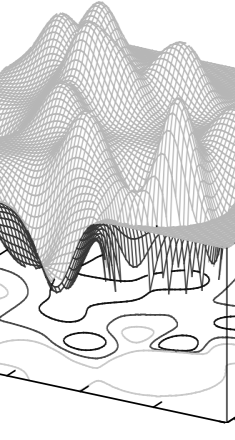
\includegraphics[height=7cm]{classPicture2-bw}
    }{\center

      \textbf{\fontsize{17}{20}\selectfont \course}

      ~

      %Lecture
      \topic\\

      \vspace{1cm}

      {\tiny~\emph{\keywords}~\\}

      \vspace{1cm}

      Marc Toussaint
      
      University of Stuttgart

      Summer 2019

      ~

    }
  }
}

\newcommand{\slide}[2]{
  \slidefont
  \incpage\begin{frame}
  \addcontentsline{toc}{section}{#1}
  \vfill
  {\headerfont #1} \vspace*{-2ex}
  \begin{itemize}\item[]~\\
    #2
  \end{itemize}
  \vfill
  \end{frame}
}

\newenvironment{slidecore}[1]{
  \slidefont\incpage
  \addcontentsline{toc}{section}{#1}
  \vfill
  {\headerfont #1} \vspace*{-2ex}
  \begin{itemize}\item[]~\\
}{
  \end{itemize}
  \vfill
}


\providecommand{\key}[1]{
  \addtocounter{mypage}{1}
% \immediate\write\keyfile{#1}
  \addtocontents{toc}{\hyperref[key:#1]{#1 (\arabic{mypage})}}
%  \phantomsection\label{key:#1}
%  \index{#1@{\hyperref[key:#1]{#1 (\arabic{mysec}:\arabic{mypage})}}|phantom}
  \addtocounter{mypage}{-1}
}

\providecommand{\course}{}

\providecommand{\subtopic}{}

\providecommand{\sublecture}[2]{
  \renewcommand{\subtopic}{#1}
  \slide{#1}{#2}
}

\providecommand{\story}[1]{
~

Motivation: {\tiny #1}\clearpage
}

\newenvironment{items}[1][9]{
\par\setlength{\unitlength}{1pt}\fontsize{#1}{#1}\linespread{1.2}\selectfont
\begin{list}{--}{\leftmargin4ex \rightmargin0ex \labelsep1ex \labelwidth2ex
\topsep0pt \parsep0ex \itemsep3pt}
}{
\end{list}
}

\providecommand{\slidesfoot}{
  \end{document}
}


  \slideshead
}

\providecommand{\exercises}{
  \newcommand{\exerciseshead}{
  \documentclass[10pt,fleqn]{article}
  \stdpackages

  \definecolor{bluecol}{rgb}{0,0,.5}
  \definecolor{greencol}{rgb}{0,.4,0}
  \definecolor{shadecolor}{gray}{0.9}
  \usepackage[
    %    pdftex%,
    %%    letterpaper,
    %    bookmarks,
    %    bookmarksnumbered,
    colorlinks,
    urlcolor=bluecol,
    citecolor=black,
    linkcolor=bluecol,
    %    pagecolor=bluecol,
    pdfborder={0 0 0},
    %pdfborderstyle={/S/U/W 1},
    %%    backref,     %link from bibliography back to sections
    %%    pagebackref, %link from bibliography back to pages
    %%    pdfstartview=FitH, %fitwidth instead of fit window
    pdfpagemode=UseNone, %UseOutlines, %bookmarks are displayed by acrobat
    pdftitle={\course},
    pdfauthor={Marc Toussaint},
    pdfkeywords={}
  ]{hyperref}
  \DeclareGraphicsExtensions{.pdf,.png,.jpg,.eps}

  \renewcommand{\r}{\varrho}
  \renewcommand{\l}{\lambda}
  \renewcommand{\L}{\Lambda}
  \renewcommand{\b}{\beta}
  \renewcommand{\d}{\delta}
  \renewcommand{\k}{\kappa}
  \renewcommand{\t}{\theta}
  \renewcommand{\O}{\Omega}
  \renewcommand{\o}{\omega}
  \renewcommand{\SS}{{\cal S}}
  \renewcommand{\=}{\!=\!}
  %\renewcommand{\boldsymbol}{}
  %\renewcommand{\Chapter}{\chapter}
  %\renewcommand{\Subsection}{\subsection}

  \renewcommand{\baselinestretch}{1.1}
  \geometry{a4paper,headsep=7mm,hdivide={15mm,*,15mm},vdivide={20mm,*,15mm}}

  \fancyhead[L]{\thetitle, \textit{Marc Toussaint}---\today}
  \fancyhead[R]{\thepage}
  \fancyhead[C]{}
  \fancyfoot{}
  \pagestyle{fancy}

  \parindent 0pt
  \parskip 0.5ex

  \newcommand{\codefont}{\helvetica{8}{1.2}{m}{n}}

  \input{../shared/macros}

  \DefineShortVerb{\@}

  \newcounter{solutions}
  \setcounter{solutions}{1}
  \newenvironment{solution}{
    \small
    \begin{shaded}
  }{
    \end{shaded}
  }
  
  \renewcommand{\hat}{\widehat}
  \newcommand{\bbg}{{\bar{\bar g}}}
  \graphicspath{{pics/}{../shared/pics/}}

  \renewcommand{\labelenumi}{{\alph{enumi})}}

  %%%%%%%%%%%%%%%%%%%%%%%%%%%%%%%%%%%%%%%%%%%%%%%%%%%%%%%%%%%%%%%%%%%%%%%%%%%%%%%%


  \mytitle{\course\\Exercise \exnum}
  \myauthor{Marc Toussaint\\ TAs: Janik Hager, Philipp Kratzer\\\small\addressUSTT}
  
  
  \begin{document}
  \onecolumn
  \maketitle
}

\newcommand{\exsection}[1]{\section{#1}}

\newcommand{\exerfoot}{
  \end{document}
}

\newenvironment{items}[1][9]{
  \par\setlength{\unitlength}{1pt}\fontsize{#1}{#1}\linespread{1.2}\selectfont
  \begin{list}{--}{\leftmargin4ex \rightmargin0ex \labelsep1ex \labelwidth2ex
      \topsep0pt \parsep0ex \itemsep3pt}
}{
  \end{list}
}

  \exerciseshead
}

\providecommand{\script}{
  \newcommand{\scripthead}{
  \documentclass[9pt,twoside]{article}
  \stdpackages

  \usepackage{palatino}
  \usepackage[envcountsect]{beamerarticle}
  \usepackage{makeidx}
  \makeindex

  \definecolor{bluecol}{rgb}{0,0,.5}
  \definecolor{greencol}{rgb}{0,.4,0}
  \definecolor{shadecolor}{gray}{0.9}
  \usepackage[
    %    pdftex%,
    %%    letterpaper,
    %bookmarks,
    bookmarksnumbered,
    colorlinks,
    urlcolor=bluecol,
    citecolor=black,
    linkcolor=bluecol,
    %    pagecolor=bluecol,
    pdfborder={0 0 0},
    %pdfborderstyle={/S/U/W 1},
    %%    backref,     %link from bibliography back to sections
    %%    pagebackref, %link from bibliography back to pages
    %%    pdfstartview=FitH, %fitwidth instead of fit window
    pdfpagemode=UseOutlines, %bookmarks are displayed by acrobat
    pdftitle={\course},
    pdfauthor={Marc Toussaint},
    pdfkeywords={}
  ]{hyperref}
  \DeclareGraphicsExtensions{.pdf,.png,.jpg,.eps}

  \usepackage{multimedia}
  %\setbeamercolor{background canvas}{bg=}

  \renewcommand{\r}{\varrho}
  \renewcommand{\l}{\lambda}
  \renewcommand{\L}{\Lambda}
  \renewcommand{\b}{\beta}
  \renewcommand{\d}{\delta}
  \renewcommand{\k}{\kappa}
  \renewcommand{\t}{\theta}
  \renewcommand{\O}{\Omega}
  \renewcommand{\o}{\omega}
  \renewcommand{\SS}{{\cal S}}
  \renewcommand{\=}{\!=\!}
  %\renewcommand{\boldsymbol}{}
  %\renewcommand{\Chapter}{\chapter}
  %\renewcommand{\Subsection}{\subsection}

  \renewcommand{\baselinestretch}{1.0}
  \geometry{a5paper,headsep=6mm,hdivide={10mm,*,10mm},vdivide={13mm,*,7mm}}

  \fancyhead[OL,ER]{\course, \textit{Marc Toussaint}}
  \fancyhead[OR,EL]{\thepage}
  \fancyhead[C]{}
  \fancyfoot{}
  \pagestyle{fancy}

%  \setcounter{tocdepth}{3}
  \setcounter{tocdepth}{2}

   \columnsep 6ex
  %  \renewcommand{\familydefault}{\sfdefault}
  \newcommand{\headerfont}{\large}%helvetica{12}{1}{b}{n}}
  \newcommand{\slidefont} {}%\helvetica{9}{1.3}{m}{n}}
  \newcommand{\storyfont} {}
  %  \renewcommand{\small}   {\helvetica{8}{1.2}{m}{n}}
  \renewcommand{\tiny}    {\footnotesize}%helvetica{7}{1.1}{m}{n}}
  \newcommand{\codefont}{\fontsize{6}{6}\selectfont}%helvetica{8}{1.2}{m}{n}}

  \input{../shared/macros}

  \DefineShortVerb{\@}

  \newcounter{solutions}
  \setcounter{solutions}{1}
  \renewenvironment{solution}{
    \small
    \begin{shaded}
  }{
    \end{shaded}
  }

  \graphicspath{{pics/}{../shared/pics/}}

%%%%%%%%%%%%%%%%%%%%%%%%%%%%%%%%%%%%%%%%%%%%%%%%%%%%%%%%%%%%%%%%%%%%%%%%%%%%%%%%

  \mytitle{\course\\Lecture Script}
  \myauthor{Marc Toussaint}

  \begin{document}

  %% \vspace*{2cm}

  \maketitle
  %\anchor{100,10}{\includegraphics[width=4cm]{optim}}

%  \vspace*{1cm}

  \emph{This is a direct concatenation and reformatting of all lecture
    slides and exercises from the \emph{Machine Learning} course (summer
    term 2019, U Stuttgart), including indexing to help
    prepare for exams.}

  \emph{Double-starred** sections and slides are not relevant for the exam.}

  {\tableofcontents}
}

%%%%%%%%%%%%%%%%%%%%%%%%%%%%%%%%%%%%%%%%%%%%%%%%%%%%%%%%%%%%%%%%%%%%%%%%%%%%%%%%

%% \renewcommand{\keywords}{}
%% \newcommand{\topic}{}
%% \renewcommand{\mypause}{}

  \newcounter{mypage}
  \setcounter{mypage}{0}
  \newcounter{mysec}
  \setcounter{mysec}{0}
  \newcommand{\incpage}{\addtocounter{mypage}{1}}
  \newcommand{\incsec} {\addtocounter{mysec}{1}}

\newcommand{\beginTocMinipage}{
  \addtocontents{toc}{\smallskip\noindent\hspace*{.036\columnwidth}}
  \addtocontents{toc}{\protect\begin{minipage}{.914\columnwidth}\small}
}
\newcommand{\closeTocMinipage}{
  \addtocontents{toc}{\protect\end{minipage}}
  \addtocontents{toc}{}
  \addtocontents{toc}{\medskip}
}

\renewcommand{\slides}[1][]{
  \clearpage
  \incsec
  \section{\topic}
  {\small #1}
  \beginTocMinipage
  \setcounter{mypage}{0}
  \smallskip\nopagebreak\hrule\medskip
}

\newcommand{\slidesfoot}{
  \closeTocMinipage
  \bigskip
}

\newcommand{\sublecture}[2]{
  \pagebreak[3]
  \incpage
  \closeTocMinipage
  \subsection{#1}
  {\storyfont #2}
  \beginTocMinipage
  {\hfill\tiny \textsf{\arabic{mysec}:\arabic{mypage}}}\nopagebreak%
  \smallskip\nopagebreak\hrule
}

\newcommand{\key}[1]{
  \pagebreak[2]
  \addtocounter{mypage}{1}
  \addtocontents{toc}{\hyperref[key:#1]{#1 (\arabic{mysec}:\arabic{mypage})}}
  \phantomsection\label{key:#1}
  \index{#1@{\hyperref[key:#1]{#1 (\arabic{mysec}:\arabic{mypage})}}|phantom}
  \addtocounter{mypage}{-1}
}

\newenvironment{slidecore}[1]{
  \incpage
  \subsubsection*{#1}%{\headerfont\noindent\textbf{#1}\\}%
  \vspace{-6ex}%
  \begin{list}{$\bullet$}{\leftmargin4ex \rightmargin0ex \labelsep1ex
    \labelwidth2ex \partopsep0ex \topsep0ex \parsep.5ex \parskip0ex \itemsep0pt}\item[]~\\\nopagebreak%
}{
  \end{list}\nopagebreak%
  {\hfill\tiny \textsf{\arabic{mysec}:\arabic{mypage}}}\nopagebreak%
  \smallskip\nopagebreak\hrule
}

\newcommand{\slide}[2]{
  \begin{slidecore}{#1}
    #2
  \end{slidecore}
}

\newcommand{\exsection}[1]{
  \subsubsection{#1}
}

\renewcommand{\exercises}{
  \subsection{Exercise \exnum}
}

\newcommand{\exerfoot}{
  \bigskip
}

\newcommand{\story}[1]{
  \subsection*{Motivation \& Outline}
  \addtocontents{toc}{\hyperref[mot\arabic{mysec}]{Motivation \& Outline}}
  \phantomsection\label{mot\arabic{mysec}}
  {\storyfont\sf #1}
  \medskip\nopagebreak\hrule
}

\newcounter{savedsection}
\newcommand{\subappendix}{\setcounter{savedsection}{\arabic{section}}\appendix}
\newcommand{\noappendix}{
  \setcounter{section}{\arabic{savedsection}}% restore section number
  \setcounter{subsection}{0}% reset section counter
%  \gdef\@chapapp{\sectionname}% reset section name
  \renewcommand{\thesection}{\arabic{section}}% make section numbers arabic
}

\newenvironment{items}[1][9]{
\par\setlength{\unitlength}{1pt}\fontsize{#1}{#1}\linespread{1.2}\selectfont
\begin{list}{--}{\leftmargin4ex \rightmargin0ex \labelsep1ex \labelwidth2ex
\topsep0pt \parsep0ex \itemsep3pt}
}{
\end{list}
}

  \scripthead
}

\providecommand{\course}{NO COURSE}
\providecommand{\topic}{NO TOPIC}
\providecommand{\keywords}{NO KEYWORDS}
\providecommand{\exnum}{NO NUMBER}


\providecommand{\stdpackages}{
  \usepackage{amsmath}
  \usepackage{amssymb}
  \usepackage{amsfonts}
  \allowdisplaybreaks
  \usepackage{amsthm}
  \usepackage{eucal}
  \usepackage{graphicx}
  \usepackage{color}
  \usepackage{geometry}
  \usepackage{framed}
%  \usecolor{xcolor}
  \definecolor{shadecolor}{gray}{0.9}
  \setlength{\FrameSep}{3pt}
  \usepackage{fancyvrb}
  \fvset{numbers=left,xleftmargin=5ex}

  \usepackage{multicol} 
  \usepackage{fancyhdr}
}

\providecommand{\addressUSTT}{
  Machine~Learning~\&~Robotics~lab, U~Stuttgart\\\small
  Universit{\"a}tsstra{\ss}e 38, 70569~Stuttgart, Germany
}


\renewcommand{\course}{Machine Learning}
\renewcommand{\topic}{Introduction}
\renewcommand{\keywords}{}

\slides

%%%%%%%%%%%%%%%%%%%%%%%%%%%%%%%%%%%%%%%%%%%%%%%%%%%%%%%%%%%%%%%%%%%%%%%%%%%%%%%%

\slide{What is Machine Learning?}{

~

%% \textbf{1)} Machine Learning is an approach to understand learning\\ ~~~ by building
%% learning systems

%% \cen{(``synthetic'' approach to a science of learning)}

%% ~\mypause

1) A long list of methods/algorithms for different data anlysis problems
\begin{items}
\item in sciences
\item in commerce
\end{items}

~

\textbf{2) Frameworks to develop your own learning algorithm/method}

~

3) Machine Learning ~ = ~ model formulation + optimization

}

%%%%%%%%%%%%%%%%%%%%%%%%%%%%%%%%%%%%%%%%%%%%%%%%%%%%%%%%%%%%%%%%%%%%%%%%%%%%%%%%

\slide{What is Machine Learning?}{

\item Pedro Domingos: \emph{A Few Useful Things to Know about Machine
Learning}

~

%\cen{LEARNING = REPRESENTATION + EVALUATION + OPTIMIZATION}
\cen{learning = representation + evaluation + optimization}

~

\item ``Representation'': Choice of model, choice of hypothesis space

\item ``Evaluation'': Choice of objective function, optimality
principle

{\small
\item[] Notes: The \emph{prior} is both, a choice of representation
and, usually, a part of the objective function.

In Bayesian settings, the choice of model often directly implies
also the ``objective function''

}

\item ``Optimization'': The algorithm to compute/approximate the best model

}

%%%%%%%%%%%%%%%%%%%%%%%%%%%%%%%%%%%%%%%%%%%%%%%%%%%%%%%%%%%%%%%%%%%%%%%%%%%%%%%%

\slide{}{

Pedro Domingos: \emph{A Few Useful Things to Know about Machine
Learning}

\item It's generalization that counts
\begin{items}
\item Data alone is not enough
\item Overfitting has many faces
\item Intuition fails in high dimensions
\item Theoretical guarantees are not what they seem
\end{items}

\item Feature engineering is the key
\item More data beats a cleverer algorithm
\item Learn many models, not just one
\item Simplicity does not imply accuracy
\item Representable does not imply learnable
\item Correlation does not imply causation
}

%%%%%%%%%%%%%%%%%%%%%%%%%%%%%%%%%%%%%%%%%%%%%%%%%%%%%%%%%%%%%%%%%%%%%%%%%%%%%%%%

\slide{What is Machine Learning?}{

\item In large parts, ML is: \quad (let's call this ML$^0$)

\cen{\emph{Fitting a function $f: x\mapsto y$ to given data $D=\{ (x_i,y_i) \}_{i=1}^n$}}

~\pause

\item Why is function fitting so omnipresent?
\pause
\begin{items}
\item Dynamics, behavior, decisions, control, predictions -- are all about functions
\item Thinking? ~ (i.e., planning, optimization, (logical) inference, CSP solving, etc?)
\item In the latter case, algorithms often provide the scaffolding, ML the heuristics to accelerate/scale them. (E.g., an evaluation function within a MCTS planning algorithm.)
\end{items}

}

%%%%%%%%%%%%%%%%%%%%%%%%%%%%%%%%%%%%%%%%%%%%%%%%%%%%%%%%%%%%%%%%%%%%%%%%%%%%%%%%

\slide{ML$^0$ objective: Empirical Risk Minimization}{

\item We have a hypothesis space $\HH$ of functions $f:x\mapsto y$

In a standard parameteric case $\HH = \{ f_\t \| \t\in\RRR^n \}$ are functions $f_\t: x \mapsto y$ that are described by $n$ parameters $\t\in\RRR^n$

~

\item Given data $D=\{ (x_i,y_i) \}_{i=1}^n$, the standard objective is to minimize the ``error'' on the data
\begin{align*}
f^* \argmin _{f\in\HH} \sum_{i=1}^n \ell(f(x_i), y_i) ~,
\end{align*}
where $\ell(\hat y, y) > 0$ penalizes a discrepancy between a model output $\hat y$ and the data $y$.

\begin{items}
\item Squared error $\ell(\hat y, y) = (\hat y - y)^2$
\item Classification error $\ell(\hat y, y) = [ \hat y \not= y ]$
\item neg-log likelihood $\ell(\hat y, y) = -\log p(y \| \hat y)$
\item etc
\end{items}

}

%%%%%%%%%%%%%%%%%%%%%%%%%%%%%%%%%%%%%%%%%%%%%%%%%%%%%%%%%%%%%%%%%%%%%%%%%%%%%%%%

\slide{What is Machine Learning beyond ML$^0$?}{

%% \item In large parts, ML is: \quad (let's call this ML$^0$)

%% \cen{\emph{Fitting a function $f: x\mapsto y$ to given data $D=\{ (x_i,y_i) \}_{i=1}^n$}}

%% ~

%% Beyond ML$^0$:

\item Fitting more structured models to data, which includes
\begin{items}
\item Time series, recurrent processes
\item Graphical Models
\item Unsupervised learning (semi-supervised learning)
\end{items}
{\small
...but in all these cases, the scenario is still not interactive, the data $D$ is static, the decision is about picking a single model $f$ from a hypothesis space, and the objective is a loss based on $f$ and $D$ only.

}

\item Active Learning, where the ``ML agent'' makes decisions about what data label to query next

\item Bandits, Reinforcement Learning, manipulating the domain (and thereby data source)

}

%%%%%%%%%%%%%%%%%%%%%%%%%%%%%%%%%%%%%%%%%%%%%%%%%%%%%%%%%%%%%%%%%%%%%%%%%%%%%%%%

\slide{Machine Learning is everywhere}{

~

NSA, Amazon, Google, Zalando, Trading, ...

Chemistry, Biology, Physics, ...

Control, Operations Reserach, Scheduling, ...

}

%%%%%%%%%%%%%%%%%%%%%%%%%%%%%%%%%%%%%%%%%%%%%%%%%%%%%%%%%%%%%%%%%%%%%%%%%%%%%%%%

\slide{Face recognition}{

~

\cen{\twocol{.3}{.4}{\center
\show{facial-recognition}
keypoints
}{\center
\show{eigenfaces}
eigenfaces
}}

~

\hfill (e.g., Viola \& Jones)

}

%%%%%%%%%%%%%%%%%%%%%%%%%%%%%%%%%%%%%%%%%%%%%%%%%%%%%%%%%%%%%%%%%%%%%%%%%%%%%%%%

\slide{Hand-written digit recognition (US postal data)}{

~

\show{digits}

~

\hfill (e.g., Yann LeCun)

}

%%%%%%%%%%%%%%%%%%%%%%%%%%%%%%%%%%%%%%%%%%%%%%%%%%%%%%%%%%%%%%%%%%%%%%%%%%%%%%%%

\slide{Gene annotation}{

~

\show[.9]{wormbase}

~

\hfill (e.g., Gunnar R\"atsch, mGene Project)

}

%%%%%%%%%%%%%%%%%%%%%%%%%%%%%%%%%%%%%%%%%%%%%%%%%%%%%%%%%%%%%%%%%%%%%%%%%%%%%%%%

\slide{Speech recognition}{

~

\show{speechRecognition}

}

%%%%%%%%%%%%%%%%%%%%%%%%%%%%%%%%%%%%%%%%%%%%%%%%%%%%%%%%%%%%%%%%%%%%%%%%%%%%%%%%

\slide{Spam filters}{

~

\show{emailSpamWords}

}

%%%%%%%%%%%%%%%%%%%%%%%%%%%%%%%%%%%%%%%%%%%%%%%%%%%%%%%%%%%%%%%%%%%%%%%%%%%%%%%%

\slide{}{

Machine Learning became an important technology\\in
science as well

~

(Stuttgart Cluster of Excellence ``Data-integrated Simulation Science (SimTech)'')

}

%%%%%%%%%%%%%%%%%%%%%%%%%%%%%%%%%%%%%%%%%%%%%%%%%%%%%%%%%%%%%%%%%%%%%%%%%%%%%%%%

%% \slide{Learning from data}{

%% \small

%% \item Predict whether a patient, hospitalized due to a heart attack, will
%% have a second heart attack. The prediction is to be based on
%% demographic, diet and clinical measurements for that patient.

%% \item Predict the price of a stock in 6 months from now, on the basis of
%% company performance measures and economic data.

%% \item Identify the numbers in a handwritten ZIP code, from a digitized
%% image.

%% \item Estimate the amount of glucose in the blood of a diabetic person,
%% from the infrared absorption spectrum of that personâs blood.

%% \item Identify the risk factors for prostate cancer, based on clinical and
%% demographic variables.

%% {\hfill\tiny (from Hastie et al)}

%% \mypause

%% \item Predict which ads/offers a web customer will follow based on his
%% history of browsing.

%% \item Recognize the words in spoken natural language.

%% \item Classify DNA snipplets to be genes or introns.

%% \item Classify an email as spam ~ (or site access as hostile attack).

%% }

%%%%%%%%%%%%%%%%%%%%%%%%%%%%%%%%%%%%%%%%%%%%%%%%%%%%%%%%%%%%%%%%%%%%%%%%%%%%%%%%

%% \slide{}{

%% Examples of ML \emph{for behavior}...

%% }

%%%%%%%%%%%%%%%%%%%%%%%%%%%%%%%%%%%%%%%%%%%%%%%%%%%%%%%%%%%%%%%%%%%%%%%%%%%%%%%%

%% \slide{Learing motor skills}{

%% ~

%% ~

%% \twocol{.5}{.4}{\center
%%   \mov{\show{mov-balance}}{05-sethu-movies/DA_PoleLearn.avi}
%% }{\center
%%   \mov{\show{mov-juggle}}{05-sethu-movies/DB_juggle.avi}
%% }

%% ~

%% \hfill (around 2000, by Schaal, Atkeson, Vijayakumar)

%% }

%%%%%%%%%%%%%%%%%%%%%%%%%%%%%%%%%%%%%%%%%%%%%%%%%%%%%%%%%%%%%%%%%%%%%%%%%%%%%%%%

%% \slide{Learning to walk}{

%% ~

%% ~

%% \mov{\show[.3]{../pics-robotics/tedrake-LearningToWalk}}{10-RoboticsLecture/tedrake-LearningToWalk.avi}

%% ~

%% \hfill{\tiny (Rus Tedrake et al.)}

%% }

%%%%%%%%%%%%%%%%%%%%%%%%%%%%%%%%%%%%%%%%%%%%%%%%%%%%%%%%%%%%%%%%%%%%%%%%%%%%%%%%

%% \slide{Learning effects of actions}{

%% ~

%% ~

%% \mov{\show[.5]{tobias-explore}}{10-relationalExploration/movie_clearance_big.avi}

%% ~

%% \hfill{(Tobias Lang \& M Toussaint)}
%% %% \mov{rel. exp. 1}{tobias1.flv}

%% %% \mov{rel. exp. 2}{tobias2.flv}

%% }

%%%%%%%%%%%%%%%%%%%%%%%%%%%%%%%%%%%%%%%%%%%%%%%%%%%%%%%%%%%%%%%%%%%%%%%%%%%%%%%%

%% \slide{Learing for robot manipulation}{


%% ~

%% ~

%% \mov{\show[.5]{robi}}{09-robi/ICRAmovie.avi}

%% ~

%% \hfill{(Toussaint et al.)}

%% }

%%%%%%%%%%%%%%%%%%%%%%%%%%%%%%%%%%%%%%%%%%%%%%%%%%%%%%%%%%%%%%%%%%%%%%%%%%%%%%%%

%% \slide{Types of ML}{

%% ~

%% \item \emph{Supervised} learning: ~ learn from ``labelled'' data $\{(x_i,y_i)\}_{i=1}^N$

%% \emph{Unsupervised} learning: ~ learn from ``unlabelled'' data $\{x_i\}_{i=0}^N$ only
%% %(density estimation)

%% \emph{Semi-supervised} learning: ~ many unlabelled data, few
%% labelled data

%% ~

%% \item \emph{Reinforcement} learning: ~ learn from data
%% $\{(s_t,a_t,r_t,s_{t\po})\}$
%% \begin{items}
%% \item learn a predictive model $(s,a) \mapsto s'$

%% \item learn to predict reward $(s,a) \mapsto r$

%% \item learn a behavior $s \mapsto a$ that maximizes reward
%% \end{items}

%% %% ~\mypause

%% %% \item generative vs.\ discriminative modelling

%% }

%%%%%%%%%%%%%%%%%%%%%%%%%%%%%%%%%%%%%%%%%%%%%%%%%%%%%%%%%%%%%%%%%%%%%%%%%%%%%%%%

\slide{Organization of this lecture}{

~

\cen{See TOC of last year's slide collection}

~

\item Part 1: The Core: Regression \& Classification

\item Part 2: The Breadth of ML methods

\item Part 3: Bayesian Methods

}

%%%%%%%%%%%%%%%%%%%%%%%%%%%%%%%%%%%%%%%%%%%%%%%%%%%%%%%%%%%%%%%%%%%%%%%%%%%%%%%%

\slide{Is this a theoretical or practical course?}{

~

Neither alone.

~\mypause

\item The goal is to teach how to design good learning algorithms

\begin{center}\tiny
data\\
$\downarrow$\\
modelling [requires theory \& practise]\\
$\downarrow$\\
algorithms [requires practise \& theory]\\
$\downarrow$\\
testing, problem identification, restart
\end{center}

}

%%%%%%%%%%%%%%%%%%%%%%%%%%%%%%%%%%%%%%%%%%%%%%%%%%%%%%%%%%%%%%%%%%%%%%%%%%%%%%%%

\slide{How much math do you need?}{

~

\item Let $L(x)= \norm{y - A x}^2$. What is
$$\argmin_x L(x)$$

~

\item Find
$$\min_x \norm{y - A x}^2 \st x_i\le 1$$

~

\item Given a discriminative function $f(x,y)$ we define
$$p(y\|x) = \frac{e^{f(y,x)}}{\sum_{y'} e^{f(y',x)}}$$

~

\item Let $A$ be the covariance matrix of a Gaussian. What does the
Singular Value Decomposition $A = V D V^\T$ tell us?


}

%%%%%%%%%%%%%%%%%%%%%%%%%%%%%%%%%%%%%%%%%%%%%%%%%%%%%%%%%%%%%%%%%%%%%%%%%%%%%%%%

\slide{How much coding do you need?}{

\item A core subject of this lecture: learning to go from principles (math) to
code

~

\item Many exercises will implement algorithms we derived in the
lecture and collect experience on small data sets

~

\item Choice of language is fully free. I support C++;
tutors might prefer Python; Octave/Matlab or R is also good choice.

}

%%%%%%%%%%%%%%%%%%%%%%%%%%%%%%%%%%%%%%%%%%%%%%%%%%%%%%%%%%%%%%%%%%%%%%%%%%%%%%%%

%% \slide{Basic regression \& classification}{

%% ~

%% \showh[.4]{codepics/cubicReg}
%% \quad
%% \showh[.4]{codepics/kernelRidgeClass}

%% ~

%% \item Regression: ~ map input $x$ to continuous value $y\in\RRR$

%% Classification: ~ map input $x$ to one of $M$ classes $y\in\{1,2,..,M\}$

%% }

%% %%%%%%%%%%%%%%%%%%%%%%%%%%%%%%%%%%%%%%%%%%%%%%%%%%%%%%%%%%%%%%%%%%%%%%%%%%%%%%%%

%% \slide{Basic regression \& classification}{

%% \item A must-know!

%% \item High practical relevance for applications
%% % (including cog.\ \& neuro sciences)

%% \item Focus on linear
%%    methods on non-linear features, regularization, cross-validation

%% \cen{``linear$|$polynomial$|$Kernel ~ Ridge$|$Lasso ~
%% Regression$|$Classification''}

%% \item Relations to SVM, GPs, feature selection

%% }

%% %%%%%%%%%%%%%%%%%%%%%%%%%%%%%%%%%%%%%%%%%%%%%%%%%%%%%%%%%%%%%%%%%%%%%%%%%%%%%%%%

%% \slide{Bayesian Modelling}{

%% ~

%% \item Mr. Holmes lives in Los Angeles. One morning when Holmes leaves
%% his house, he realizes that his grass is wet. Is it due to rain, or
%% has he forgotten to turn off his sprinkler?

%% %% \item Calculate $P(R|H)$, $P(S|H)$ and compare these values to the
%% %%  prior probabilities

%% %% \item Calculate $P(R, S|H)$. $R$ and $S$ are marginally independent,
%% %%  but conditionally dependent

%% \item Holmes checks Watson’s grass, and finds it is also
%% wet. What does that imply on rain vs.\ sprinkler?

%% %Calculate $P(R|H,W)$, $P(S|H,W)$

%% ~

%% \begin{center}
%% \input{figs/vl2-rain}
%% \end{center}
%% $
%% \iff ~ P(H,W,S,R) = P(H|S,R)~ P(W|R)~ P(S)~ P(R)
%% $


%% }

%%%%%%%%%%%%%%%%%%%%%%%%%%%%%%%%%%%%%%%%%%%%%%%%%%%%%%%%%%%%%%%%%%%%%%%%%%%%%%%%

%% \slide{Bayesian Modelling}{

%% the ASIA network: a model for lung disease
%% \begin{center}
%% \input{figs/vl2-asia}
%% \end{center}
%% $\iff
%% P(D,X,E,B,L,T,S,A) =
%% P(D|E,B)~ P(X|E)~ P(E|T,L)~ P(B|S)~ P(L|S)~ P(T|A)~ P(S)~ P(A)
%% $

%% ~

%% ~

%% \twocol{.5}{.5}{
%% $A$=trip to asia\\
%% $S$=smoking\\
%% $T$=Tuberculosis\\
%% $L$=lung cancer
%% }{
%% $E$=abnormality in chest\\
%% $X$=X-ray\\
%% $D$=Dyspnea\\
%% $B$=Bronchitis
%% }

%% }

%%%%%%%%%%%%%%%%%%%%%%%%%%%%%%%%%%%%%%%%%%%%%%%%%%%%%%%%%%%%%%%%%%%%%%%%%%%%%%%%

%% \slide{Bayesian modelling}{

%% \item Fundamental view on information processing and learning

%% ~

%% \item Provides general tools for formulating structured probabilistic
%%    models

%% ~~ (e.g., latent variables, mixtures, hierarchical,
%%    deep models)

%% $\to$ a framework for formulating novel learning algorithms

%% ~

%% \item Bayesian view on linear models + regularization

%% -- regularization $\oto$ prior, ``error'' $\oto$ likelihood

%% %% ~

%% %% \item I'll introduce basics: Bayes, likelihood maximization, MAP,
%% %%    EM, Bayes Nets \& probabilistic inference

%% %% <li> Bayesian modelling and reasoning
%% %% <li> Regression & Gaussian Processes
%% %% <li> Bayesian Networks
%% %% <li> Probabilistic Inference
%% %% <li> Sampling & Approximate Inference
%% %% <li> Decision Theory & Reinforcement Learning 

%% }

%% %%%%%%%%%%%%%%%%%%%%%%%%%%%%%%%%%%%%%%%%%%%%%%%%%%%%%%%%%%%%%%%%%%%%%%%%%%%%%%%%

%% \slide{Reinforcement Learning (another course..)}{

%% \moviex{[PacMan]}{movs/Reinforcement_learning_agent_plays_Ms._Pac-Man.mp4}

%% ~

%% ~

%% I Szita, A Lorincz:
%% \emph{Learning to Play Using Low-Complexity Rule-Based Policies:
%% Illustrations through Ms. Pac-Man.} JAIR 2007.

%% }

%% %%%%%%%%%%%%%%%%%%%%%%%%%%%%%%%%%%%%%%%%%%%%%%%%%%%%%%%%%%%%%%%%%%%%%%%%%%%%%%%%

%% \slide{Reinforcement Learning (another course..)}{

%% \item Behavior!, learning to act

%% \item Basic RL methods (Temporal Difference, Q-learning, traces)

%% \item Regression in RL, Bayesian methods in RL

%% \item Applications

%% %% -- Current research often asks: Do humans/animals take decisions in a
%% %%    Bayesian way? What does that mean anyway? Is this Q meaningful, or
%% %%    is it like asking ``do humans/animals use information processing''?

%% }

%%%%%%%%%%%%%%%%%%%%%%%%%%%%%%%%%%%%%%%%%%%%%%%%%%%%%%%%%%%%%%%%%%%%%%%%%%%%%%%%

\slide{Books}{

~

\twocol{.4}{.5}{
\show{HastieEtAl}
}{

Trevor Hastie, Robert Tibshirani and Jerome Friedman:
\emph{The Elements of Statistical Learning: Data Mining, Inference,
and Prediction} Springer, Second Edition, 2009.

\url{http://www-stat.stanford.edu/~tibs/ElemStatLearn/}

(recommended: read introductory chapter)

}

~

~

\hfill \tiny(this course will not go to the full depth in math of Hastie et al.)

}

%%%%%%%%%%%%%%%%%%%%%%%%%%%%%%%%%%%%%%%%%%%%%%%%%%%%%%%%%%%%%%%%%%%%%%%%%%%%%%%%

\slide{Books}{

~

\twocol{.4}{.5}{
\show{Bishop}
}{

Bishop, C. M.: \emph{Pattern Recognition and Machine Learning}.

Springer, 2006


\url{http://research.microsoft.com/en-us/um/people/cmbishop/prml/}

(some chapters are fully online) 

}

}

%%%%%%%%%%%%%%%%%%%%%%%%%%%%%%%%%%%%%%%%%%%%%%%%%%%%%%%%%%%%%%%%%%%%%%%%%%%%%%%%

\slide{Books \& Readings}{

~

\item more recently:
\begin{items}
\item David Barber: Bayesian Reasoning and Machine Learning
\item Kevin Murphy: Machine learning: a Probabilistic Perspective
\end{items}

~

\item See the readings at the bottom of:

\cen{\tiny\url{http://ipvs.informatik.uni-stuttgart.de/mlr/marc/teaching/index.html\#readings}}

}

%%%%%%%%%%%%%%%%%%%%%%%%%%%%%%%%%%%%%%%%%%%%%%%%%%%%%%%%%%%%%%%%%%%%%%%%%%%%%%%%

%% \slide{Books}{

%% ~

%% \twocol{.4}{.5}{
%% \show{SuttonBarto}
%% }{


%% Richard S. Sutton and Andrew G. Barto: \emph{Reinforcement Learning:
%% An Introduction}. MIT Press, 1998.


%% \url{http://www.cse.iitm.ac.in/~cs670/book/the-book.html}

%% }

%% }

%%%%%%%%%%%%%%%%%%%%%%%%%%%%%%%%%%%%%%%%%%%%%%%%%%%%%%%%%%%%%%%%%%%%%%%%%%%%%%%%

\slide{Organization}{\label{lastpage}

\item Course Webpage:

\cen{\tiny\url{http://ipvs.informatik.uni-stuttgart.de/mlr/marc/teaching/19-MachineLearning/}}
\begin{items}
\item Slides, Exercises \& Software (C++)
\item Links to books and other resources
\end{items}

\item Admin things, please first ask:

  Carola Stahl, {\tiny\tt
  Carola.Stahl\@ipvs.uni-stuttgart.de}, Raum 2.217

~

\item Rules for the tutorials:

\begin{items}
\item Doing the exercises is crucial!

\item \textbf{Nur Votieraufgaben.} At the beginning of each tutorial:

-- sign into a list

-- vote on exercises you have (successfully) worked on

\item Students are randomly selected to present their solutions

\item {\color{red}You need 50\% of completed exercises to be allowed
to the exam}

\item Please check 2 weeks before the end of the term, if you can take
the exam
\end{items}

}


%%%%%%%%%%%%%%%%%%%%%%%%%%%%%%%%%%%%%%%%%%%%%%%%%%%%%%%%%%%%%%%%%%%%%%%%%%%%%%%%

%% \slide{Organisation}{

%% %\item Bitte in beidem, KVV \& Campus Management anmeldem.


%% ~

%% \item Klausur:

%% -- Dienstag 10.7.2012, 14-16h

%% }

%%%%%%%%%%%%%%%%%%%%%%%%%%%%%%%%%%%%%%%%%%%%%%%%%%%%%%%%%%%%%%%%%%%%%%%%%%%%%%%%

\slidesfoot

\providecommand{\slides}{
  \newcommand{\slideshead}{
  \newcommand{\thepage}{\arabic{mypage}}
  %beamer
  \documentclass[t,hyperref={bookmarks=true}]{beamer}
%  \documentclass[t,hyperref={bookmarks=true},aspectratio=169]{beamer}
  \setbeamersize{text margin left=5mm}
  \setbeamersize{text margin right=5mm}
  \usetheme{default}
  \usefonttheme[onlymath]{serif}
  \setbeamertemplate{navigation symbols}{}
  \setbeamertemplate{itemize items}{{\color{black}$\bullet$}}

  \newwrite\keyfile

  %\usepackage{palatino}
  \stdpackages
  \usepackage{multimedia}

  %%% geometry/spacing issues
  %
  \definecolor{bluecol}{rgb}{0,0,.5}
  \definecolor{greencol}{rgb}{0,.6,0}
  %\renewcommand{\baselinestretch}{1.1}
  \renewcommand{\arraystretch}{1.2}
  \columnsep 0mm

  \columnseprule 0pt
  \parindent 0ex
  \parskip 0ex
  %\setlength{\itemparsep}{3ex}
  %\renewcommand{\labelitemi}{\rule[3pt]{10pt}{10pt}~}
  %\renewcommand{\labelenumi}{\textbf{(\arabic{enumi})}}
  \newcommand{\headerfont}{\helvetica{13}{1.5}{b}{n}}
  \newcommand{\slidefont} {\helvetica{10}{1.4}{m}{n}}
  \newcommand{\codefont} {\helvetica{8}{1.2}{m}{n}}
  \renewcommand{\small} {\helvetica{9}{1.4}{m}{n}}
  \renewcommand{\tiny} {\helvetica{8}{1.3}{m}{n}}
  \newcommand{\ttiny} {\helvetica{7}{1.3}{m}{n}}

  %%% count pages properly and put the page number in bottom right
  %
  \newcounter{mypage}
  \newcommand{\incpage}{\addtocounter{mypage}{1}\setcounter{page}{\arabic{mypage}}}
  \setcounter{mypage}{0}
  \resetcounteronoverlays{page}

  \pagestyle{fancy}
  %\setlength{\headsep}{10mm}
  %\addtolength{\footheight}{15mm}
  \renewcommand{\headrulewidth}{0pt} %1pt}
  \renewcommand{\footrulewidth}{0pt} %.5pt}
  \cfoot{}
  \rhead{}
  \lhead{}
%  \rfoot{{\tiny\textsf{AI -- \topic -- \subtopic -- \arabic{mypage}/\pageref{lastpage}}}}
%  \rfoot{\vspace*{-4.5mm}{\tiny\textsf{\topic\ -- \subtopic\ -- \arabic{mypage}/\pageref{lastpage}}}\hspace*{-4mm}}
  \rfoot{\vspace*{-4.5mm}{\tiny\textsf{\color{gray}\topic\ -- \subtopic\ -- \arabic{mypage}/\pageref{lastpage}}}\hspace*{-4mm}}
  %\lfoot{\raisebox{5mm}{\tiny\textsf{\slideauthor}}}
  %\rfoot{\raisebox{5mm}{\tiny\textsf{\slidevenue{} -- \arabic{mypage}/\pageref{lastpage}}}}
  %\rfoot{~\anchor{30,12}{\tiny\textsf{\thepage/\pageref{lastpage}}}}
  %\lfoot{\small\textsf{Marc Toussaint}}

  \definecolor{grey}{rgb}{.8,.8,.8}
  \definecolor{head}{rgb}{.85,.9,.9}
  \definecolor{blue}{rgb}{.0,.0,.5}
  \definecolor{green}{rgb}{.0,.5,.0}
  \definecolor{red}{rgb}{.8,.0,.0}
  \newcommand{\inverted}{
    \definecolor{main}{rgb}{1,1,1}
    \color{main}
    \pagecolor[rgb]{.3,.3,.3}
  }
  \input{../shared/macros}

  \graphicspath{{pics/}{../shared/pics/}}

  \title{Machine Learning \topic}
  \author{Marc Toussaint}
  \institute{Machine Learning \& Robotics Lab, U Stuttgart}

  \begin{document}

  \rfoot{\vspace*{-5mm}{\tiny
  \textsf{\arabic{mypage}/\pageref{lastpage}}}\hspace*{-4mm}}

  %% title slide!
  \slide{}{
    \thispagestyle{empty}

    \twocol{.27}{.6}{
      \hspace*{-15mm}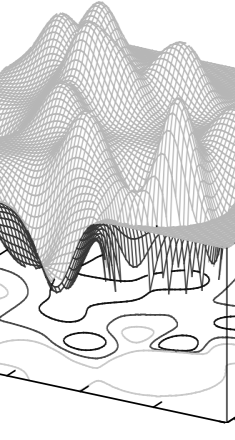
\includegraphics[height=7cm]{classPicture2-bw}
    }{\center

      \textbf{\fontsize{17}{20}\selectfont \course}

      ~

      %Lecture
      \topic\\

      \vspace{1cm}

      {\tiny~\emph{\keywords}~\\}

      \vspace{1cm}

      Marc Toussaint
      
      University of Stuttgart

      Summer 2019

      ~

    }
  }
}

\newcommand{\slide}[2]{
  \slidefont
  \incpage\begin{frame}
  \addcontentsline{toc}{section}{#1}
  \vfill
  {\headerfont #1} \vspace*{-2ex}
  \begin{itemize}\item[]~\\
    #2
  \end{itemize}
  \vfill
  \end{frame}
}

\newenvironment{slidecore}[1]{
  \slidefont\incpage
  \addcontentsline{toc}{section}{#1}
  \vfill
  {\headerfont #1} \vspace*{-2ex}
  \begin{itemize}\item[]~\\
}{
  \end{itemize}
  \vfill
}


\providecommand{\key}[1]{
  \addtocounter{mypage}{1}
% \immediate\write\keyfile{#1}
  \addtocontents{toc}{\hyperref[key:#1]{#1 (\arabic{mypage})}}
%  \phantomsection\label{key:#1}
%  \index{#1@{\hyperref[key:#1]{#1 (\arabic{mysec}:\arabic{mypage})}}|phantom}
  \addtocounter{mypage}{-1}
}

\providecommand{\course}{}

\providecommand{\subtopic}{}

\providecommand{\sublecture}[2]{
  \renewcommand{\subtopic}{#1}
  \slide{#1}{#2}
}

\providecommand{\story}[1]{
~

Motivation: {\tiny #1}\clearpage
}

\newenvironment{items}[1][9]{
\par\setlength{\unitlength}{1pt}\fontsize{#1}{#1}\linespread{1.2}\selectfont
\begin{list}{--}{\leftmargin4ex \rightmargin0ex \labelsep1ex \labelwidth2ex
\topsep0pt \parsep0ex \itemsep3pt}
}{
\end{list}
}

\providecommand{\slidesfoot}{
  \end{document}
}


  \slideshead
}

\providecommand{\exercises}{
  \newcommand{\exerciseshead}{
  \documentclass[10pt,fleqn]{article}
  \stdpackages

  \definecolor{bluecol}{rgb}{0,0,.5}
  \definecolor{greencol}{rgb}{0,.4,0}
  \definecolor{shadecolor}{gray}{0.9}
  \usepackage[
    %    pdftex%,
    %%    letterpaper,
    %    bookmarks,
    %    bookmarksnumbered,
    colorlinks,
    urlcolor=bluecol,
    citecolor=black,
    linkcolor=bluecol,
    %    pagecolor=bluecol,
    pdfborder={0 0 0},
    %pdfborderstyle={/S/U/W 1},
    %%    backref,     %link from bibliography back to sections
    %%    pagebackref, %link from bibliography back to pages
    %%    pdfstartview=FitH, %fitwidth instead of fit window
    pdfpagemode=UseNone, %UseOutlines, %bookmarks are displayed by acrobat
    pdftitle={\course},
    pdfauthor={Marc Toussaint},
    pdfkeywords={}
  ]{hyperref}
  \DeclareGraphicsExtensions{.pdf,.png,.jpg,.eps}

  \renewcommand{\r}{\varrho}
  \renewcommand{\l}{\lambda}
  \renewcommand{\L}{\Lambda}
  \renewcommand{\b}{\beta}
  \renewcommand{\d}{\delta}
  \renewcommand{\k}{\kappa}
  \renewcommand{\t}{\theta}
  \renewcommand{\O}{\Omega}
  \renewcommand{\o}{\omega}
  \renewcommand{\SS}{{\cal S}}
  \renewcommand{\=}{\!=\!}
  %\renewcommand{\boldsymbol}{}
  %\renewcommand{\Chapter}{\chapter}
  %\renewcommand{\Subsection}{\subsection}

  \renewcommand{\baselinestretch}{1.1}
  \geometry{a4paper,headsep=7mm,hdivide={15mm,*,15mm},vdivide={20mm,*,15mm}}

  \fancyhead[L]{\thetitle, \textit{Marc Toussaint}---\today}
  \fancyhead[R]{\thepage}
  \fancyhead[C]{}
  \fancyfoot{}
  \pagestyle{fancy}

  \parindent 0pt
  \parskip 0.5ex

  \newcommand{\codefont}{\helvetica{8}{1.2}{m}{n}}

  \input{../shared/macros}

  \DefineShortVerb{\@}

  \newcounter{solutions}
  \setcounter{solutions}{1}
  \newenvironment{solution}{
    \small
    \begin{shaded}
  }{
    \end{shaded}
  }
  
  \renewcommand{\hat}{\widehat}
  \newcommand{\bbg}{{\bar{\bar g}}}
  \graphicspath{{pics/}{../shared/pics/}}

  \renewcommand{\labelenumi}{{\alph{enumi})}}

  %%%%%%%%%%%%%%%%%%%%%%%%%%%%%%%%%%%%%%%%%%%%%%%%%%%%%%%%%%%%%%%%%%%%%%%%%%%%%%%%


  \mytitle{\course\\Exercise \exnum}
  \myauthor{Marc Toussaint\\ TAs: Janik Hager, Philipp Kratzer\\\small\addressUSTT}
  
  
  \begin{document}
  \onecolumn
  \maketitle
}

\newcommand{\exsection}[1]{\section{#1}}

\newcommand{\exerfoot}{
  \end{document}
}

\newenvironment{items}[1][9]{
  \par\setlength{\unitlength}{1pt}\fontsize{#1}{#1}\linespread{1.2}\selectfont
  \begin{list}{--}{\leftmargin4ex \rightmargin0ex \labelsep1ex \labelwidth2ex
      \topsep0pt \parsep0ex \itemsep3pt}
}{
  \end{list}
}

  \exerciseshead
}

\providecommand{\script}{
  \newcommand{\scripthead}{
  \documentclass[9pt,twoside]{article}
  \stdpackages

  \usepackage{palatino}
  \usepackage[envcountsect]{beamerarticle}
  \usepackage{makeidx}
  \makeindex

  \definecolor{bluecol}{rgb}{0,0,.5}
  \definecolor{greencol}{rgb}{0,.4,0}
  \definecolor{shadecolor}{gray}{0.9}
  \usepackage[
    %    pdftex%,
    %%    letterpaper,
    %bookmarks,
    bookmarksnumbered,
    colorlinks,
    urlcolor=bluecol,
    citecolor=black,
    linkcolor=bluecol,
    %    pagecolor=bluecol,
    pdfborder={0 0 0},
    %pdfborderstyle={/S/U/W 1},
    %%    backref,     %link from bibliography back to sections
    %%    pagebackref, %link from bibliography back to pages
    %%    pdfstartview=FitH, %fitwidth instead of fit window
    pdfpagemode=UseOutlines, %bookmarks are displayed by acrobat
    pdftitle={\course},
    pdfauthor={Marc Toussaint},
    pdfkeywords={}
  ]{hyperref}
  \DeclareGraphicsExtensions{.pdf,.png,.jpg,.eps}

  \usepackage{multimedia}
  %\setbeamercolor{background canvas}{bg=}

  \renewcommand{\r}{\varrho}
  \renewcommand{\l}{\lambda}
  \renewcommand{\L}{\Lambda}
  \renewcommand{\b}{\beta}
  \renewcommand{\d}{\delta}
  \renewcommand{\k}{\kappa}
  \renewcommand{\t}{\theta}
  \renewcommand{\O}{\Omega}
  \renewcommand{\o}{\omega}
  \renewcommand{\SS}{{\cal S}}
  \renewcommand{\=}{\!=\!}
  %\renewcommand{\boldsymbol}{}
  %\renewcommand{\Chapter}{\chapter}
  %\renewcommand{\Subsection}{\subsection}

  \renewcommand{\baselinestretch}{1.0}
  \geometry{a5paper,headsep=6mm,hdivide={10mm,*,10mm},vdivide={13mm,*,7mm}}

  \fancyhead[OL,ER]{\course, \textit{Marc Toussaint}}
  \fancyhead[OR,EL]{\thepage}
  \fancyhead[C]{}
  \fancyfoot{}
  \pagestyle{fancy}

%  \setcounter{tocdepth}{3}
  \setcounter{tocdepth}{2}

   \columnsep 6ex
  %  \renewcommand{\familydefault}{\sfdefault}
  \newcommand{\headerfont}{\large}%helvetica{12}{1}{b}{n}}
  \newcommand{\slidefont} {}%\helvetica{9}{1.3}{m}{n}}
  \newcommand{\storyfont} {}
  %  \renewcommand{\small}   {\helvetica{8}{1.2}{m}{n}}
  \renewcommand{\tiny}    {\footnotesize}%helvetica{7}{1.1}{m}{n}}
  \newcommand{\codefont}{\fontsize{6}{6}\selectfont}%helvetica{8}{1.2}{m}{n}}

  \input{../shared/macros}

  \DefineShortVerb{\@}

  \newcounter{solutions}
  \setcounter{solutions}{1}
  \renewenvironment{solution}{
    \small
    \begin{shaded}
  }{
    \end{shaded}
  }

  \graphicspath{{pics/}{../shared/pics/}}

%%%%%%%%%%%%%%%%%%%%%%%%%%%%%%%%%%%%%%%%%%%%%%%%%%%%%%%%%%%%%%%%%%%%%%%%%%%%%%%%

  \mytitle{\course\\Lecture Script}
  \myauthor{Marc Toussaint}

  \begin{document}

  %% \vspace*{2cm}

  \maketitle
  %\anchor{100,10}{\includegraphics[width=4cm]{optim}}

%  \vspace*{1cm}

  \emph{This is a direct concatenation and reformatting of all lecture
    slides and exercises from the \emph{Machine Learning} course (summer
    term 2019, U Stuttgart), including indexing to help
    prepare for exams.}

  \emph{Double-starred** sections and slides are not relevant for the exam.}

  {\tableofcontents}
}

%%%%%%%%%%%%%%%%%%%%%%%%%%%%%%%%%%%%%%%%%%%%%%%%%%%%%%%%%%%%%%%%%%%%%%%%%%%%%%%%

%% \renewcommand{\keywords}{}
%% \newcommand{\topic}{}
%% \renewcommand{\mypause}{}

  \newcounter{mypage}
  \setcounter{mypage}{0}
  \newcounter{mysec}
  \setcounter{mysec}{0}
  \newcommand{\incpage}{\addtocounter{mypage}{1}}
  \newcommand{\incsec} {\addtocounter{mysec}{1}}

\newcommand{\beginTocMinipage}{
  \addtocontents{toc}{\smallskip\noindent\hspace*{.036\columnwidth}}
  \addtocontents{toc}{\protect\begin{minipage}{.914\columnwidth}\small}
}
\newcommand{\closeTocMinipage}{
  \addtocontents{toc}{\protect\end{minipage}}
  \addtocontents{toc}{}
  \addtocontents{toc}{\medskip}
}

\renewcommand{\slides}[1][]{
  \clearpage
  \incsec
  \section{\topic}
  {\small #1}
  \beginTocMinipage
  \setcounter{mypage}{0}
  \smallskip\nopagebreak\hrule\medskip
}

\newcommand{\slidesfoot}{
  \closeTocMinipage
  \bigskip
}

\newcommand{\sublecture}[2]{
  \pagebreak[3]
  \incpage
  \closeTocMinipage
  \subsection{#1}
  {\storyfont #2}
  \beginTocMinipage
  {\hfill\tiny \textsf{\arabic{mysec}:\arabic{mypage}}}\nopagebreak%
  \smallskip\nopagebreak\hrule
}

\newcommand{\key}[1]{
  \pagebreak[2]
  \addtocounter{mypage}{1}
  \addtocontents{toc}{\hyperref[key:#1]{#1 (\arabic{mysec}:\arabic{mypage})}}
  \phantomsection\label{key:#1}
  \index{#1@{\hyperref[key:#1]{#1 (\arabic{mysec}:\arabic{mypage})}}|phantom}
  \addtocounter{mypage}{-1}
}

\newenvironment{slidecore}[1]{
  \incpage
  \subsubsection*{#1}%{\headerfont\noindent\textbf{#1}\\}%
  \vspace{-6ex}%
  \begin{list}{$\bullet$}{\leftmargin4ex \rightmargin0ex \labelsep1ex
    \labelwidth2ex \partopsep0ex \topsep0ex \parsep.5ex \parskip0ex \itemsep0pt}\item[]~\\\nopagebreak%
}{
  \end{list}\nopagebreak%
  {\hfill\tiny \textsf{\arabic{mysec}:\arabic{mypage}}}\nopagebreak%
  \smallskip\nopagebreak\hrule
}

\newcommand{\slide}[2]{
  \begin{slidecore}{#1}
    #2
  \end{slidecore}
}

\newcommand{\exsection}[1]{
  \subsubsection{#1}
}

\renewcommand{\exercises}{
  \subsection{Exercise \exnum}
}

\newcommand{\exerfoot}{
  \bigskip
}

\newcommand{\story}[1]{
  \subsection*{Motivation \& Outline}
  \addtocontents{toc}{\hyperref[mot\arabic{mysec}]{Motivation \& Outline}}
  \phantomsection\label{mot\arabic{mysec}}
  {\storyfont\sf #1}
  \medskip\nopagebreak\hrule
}

\newcounter{savedsection}
\newcommand{\subappendix}{\setcounter{savedsection}{\arabic{section}}\appendix}
\newcommand{\noappendix}{
  \setcounter{section}{\arabic{savedsection}}% restore section number
  \setcounter{subsection}{0}% reset section counter
%  \gdef\@chapapp{\sectionname}% reset section name
  \renewcommand{\thesection}{\arabic{section}}% make section numbers arabic
}

\newenvironment{items}[1][9]{
\par\setlength{\unitlength}{1pt}\fontsize{#1}{#1}\linespread{1.2}\selectfont
\begin{list}{--}{\leftmargin4ex \rightmargin0ex \labelsep1ex \labelwidth2ex
\topsep0pt \parsep0ex \itemsep3pt}
}{
\end{list}
}

  \scripthead
}

\providecommand{\course}{NO COURSE}
\providecommand{\topic}{NO TOPIC}
\providecommand{\keywords}{NO KEYWORDS}
\providecommand{\exnum}{NO NUMBER}


\providecommand{\stdpackages}{
  \usepackage{amsmath}
  \usepackage{amssymb}
  \usepackage{amsfonts}
  \allowdisplaybreaks
  \usepackage{amsthm}
  \usepackage{eucal}
  \usepackage{graphicx}
  \usepackage{color}
  \usepackage{geometry}
  \usepackage{framed}
%  \usecolor{xcolor}
  \definecolor{shadecolor}{gray}{0.9}
  \setlength{\FrameSep}{3pt}
  \usepackage{fancyvrb}
  \fvset{numbers=left,xleftmargin=5ex}

  \usepackage{multicol} 
  \usepackage{fancyhdr}
}

\providecommand{\addressUSTT}{
  Machine~Learning~\&~Robotics~lab, U~Stuttgart\\\small
  Universit{\"a}tsstra{\ss}e 38, 70569~Stuttgart, Germany
}


\renewcommand{\course}{Robotics}
\renewcommand{\coursepicture}{roboticsLecture}
\renewcommand{\coursedate}{Winter 2014}
\renewcommand{\topic}{Kinematics}

\slides

%%%%%%%%%%%%%%%%%%%%%%%%%%%%%%%%%%%%%%%%%%%%%%%%%%%%%%%%%%%%%%%%%%%%%%%%%%%%%%%%
\key{Mobile robotics vs. Manipulation vs. Kinematic/Dynamic motion control}
\slide{}{

\item Two ``types of robotics'':

1) Mobile robotics ~ -- ~ is all about localization \& mapping

2) Manipulation ~ -- ~ is all about interacting with the world

0) Kinematic/Dynamic Motion Control: same as 2) without ever making it
to interaction..

~

\item Typical manipulation robots (and animals) are kinematic trees

Their pose/state is described by all joint angles

}

%%%%%%%%%%%%%%%%%%%%%%%%%%%%%%%%%%%%%%%%%%%%%%%%%%%%%%%%%%%%%%%%%%%%%%%%%%%%%%%%

\slide{Basic motion generation problem}{

\item Move all joints in a coordinated way so that the endeffector
makes a desired movement

~

\show[.4]{multiTask}

\hfill\tiny\texttt{01-kinematics: ./x.exe -mode 2/3/4}

}

%%%%%%%%%%%%%%%%%%%%%%%%%%%%%%%%%%%%%%%%%%%%%%%%%%%%%%%%%%%%%%%%%%%%%%%%%%%%%%%%

\slide{Outline}{

~

\item Basic 3D geometry and notation

~

\item Kinematics:~ $\phi:~ q \mapsto y$

\item Inverse Kinematics:~ $y^* \mapsto q^* = \argmin_q \norm{\phi(q) - y^*}^2_C + \norm{q-q_0}^2_W$

\item Basic motion heuristics:~ Motion profiles

~

\item Additional things to know
\begin{items}
\item Many simultaneous task variables
\item Singularities, null space, 
\end{items}

}

%%%%%%%%%%%%%%%%%%%%%%%%%%%%%%%%%%%%%%%%%%%%%%%%%%%%%%%%%%%%%%%%%%%%%%%%%%%%%%%%
\sublecture{Basic 3D geometry \& notation}

%%%%%%%%%%%%%%%%%%%%%%%%%%%%%%%%%%%%%%%%%%%%%%%%%%%%%%%%%%%%%%%%%%%%%%%%%%%%%%%%

\slide{Pose (position \& orientation)}{

\shows[.5]{geo-3D-3}

\item A \emph{pose} is described by a translation $p\in\RRR^3$ and a rotation $R\in SO(3)$
\begin{items}
\item $R$ is an \emph{orthonormal} matrix (orthogonal vectors stay orthogonal, unit vectors stay unit)
\item $R^\1 = R^\T$
\item columns and rows are orthogonal unit vectors
\item $\det(R) = 1$
\item $
R = \mat{ccc}{
  R_{11} & R_{12} & R_{13} \\
  R_{21} & R_{22} & R_{23} \\
  R_{31} & R_{32} & R_{33}}
$
\end{items}

}

%%%%%%%%%%%%%%%%%%%%%%%%%%%%%%%%%%%%%%%%%%%%%%%%%%%%%%%%%%%%%%%%%%%%%%%%%%%%%%%%
%% \slide{Rotation matrix: examples}{

%% \item 3D:
%% \begin{align*}
%% R_z(\t) &= \mat{ccc}{ \cos\t & -\sin\t & 0 \\  \sin\t & \cos\t & 0 \\ 0 & 0 & 1} \\
%% R_y(\t) &= \mat{ccc}{ \cos\t & 0 &  \sin\t \\ 0 & 1 & 0 \\ -\sin\t & 0 & \cos\t} \\
%% R_x(\t) &= \mat{ccc}{ 1 & 0 & 0 \\ 0 & \cos\t & -\sin\t \\ 0 &  \sin\t & \cos\t}
%% \end{align*}


%% \item $\RRR^{3 \times 3}$ has 9 numbers

%% \item 6 constraints ~ (3 orthogonal, 3 normal)

%% \item 3 DoF

%% }

%%%%%%%%%%%%%%%%%%%%%%%%%%%%%%%%%%%%%%%%%%%%%%%%%%%%%%%%%%%%%%%%%%%%%%%%%%%%%%%%
\key{Coordinate frames and transforms}
\slide{Frame and coordinate transforms}{

\shows[.5]{geo-3D-4}

\item Let $(\vec o,\vec e_{1:3})$ be the world frame, $(\vec o',\vec e'_{1:3})$ be the body's frame.

The new basis vectors are the \emph{columns} in $R$, that is, $\vec
e_1' = R_{11} \vec e_1 + R_{21} \vec e_2 + R_{31} \vec e_3$, etc,


\item
$x$ = coordinates in world frame $(\vec o,\vec e_{1:3})$

$x'$ = coordinates in body frame $(\vec o',\vec e'_{1:3})$

$p$ = coordinates of $\vec o'$ in world frame $(\vec o,\vec e_{1:3})$
$$x = p + R x'$$

}

%%%%%%%%%%%%%%%%%%%%%%%%%%%%%%%%%%%%%%%%%%%%%%%%%%%%%%%%%%%%%%%%%%%%%%%%%%%%%%%%

\slide{Briefly: Alternative Rotation Representations}{

~

(See the ``geometry notes'' for more details!)

}

%%%%%%%%%%%%%%%%%%%%%%%%%%%%%%%%%%%%%%%%%%%%%%%%%%%%%%%%%%%%%%%%%%%%%%%%%%%%%%%%
\slide{Euler angles}{

\item Describe rotation by consecutive rotation about different axis:
\begin{items}
\item 3-1-3 or 3-1-2 conventions, yaw-pitch-roll (3-2-1) in air flight
\item first rotate $\p$ about $\vec e_3$, then $\t$ about the {new}
  $\vec e_1'$, then $\psi$ about the {new} $\vec e_3''$
\end{items}

\item Gimbal Lock

\show[.3]{gimbal}

\item Euler angles have severe problem:
\begin{items}
\item if two axes align: blocks 1 DoF of rotation!!
\item ``singularity'' of Euler angles
\item Example: 3-1-3 and second rotation 0 or $\pi$
\end{items}

}

%%%%%%%%%%%%%%%%%%%%%%%%%%%%%%%%%%%%%%%%%%%%%%%%%%%%%%%%%%%%%%%%%%%%%%%%%%%%%%%%
\slide{Rotation vector}{

\item vector $w \in \RRR^3$
\begin{items}
\item length $|w|=\theta$  is rotation angle (in radians)
\item direction of $w$ = rotation axis ($\ubar w=w/\t$)
\end{items}

\item Application on a vector $v$ (Rodrigues' formula):
\begin{align*}
w \cdot v
  = \cos\t~ v
  + \sin\t~ (\ubar w\times v)
  + (1-\cos\t)~ \ubar w(\ubar w^\T v)
\end{align*}

\item Conversion to matrix:
\begin{align*}
R(w)
 &= \exp(\hat w) \\
 &= \cos\t~ I + \sin\t~ \hat w/\t + (1-\cos\t)~ w w^\T/\t^2 \\
\hat w &:= \mat{ccc}{0 & -w_3 & w_2 \\ w_3 & 0 & -w_1 \\-w_2 & w_1 & 0}
\end{align*}
($\hat w$ is called skew matrix, with property $\hat w v = w \times
v$; $\exp(\cdot)$ is called exponential map)

\item Composition: convert to matrix first

\item Drawback: singularity for small rotations

}

%%%%%%%%%%%%%%%%%%%%%%%%%%%%%%%%%%%%%%%%%%%%%%%%%%%%%%%%%%%%%%%%%%%%%%%%%%%%%%%%

\slide{Quaternion}{

\item A quaternion is $r\in\RRR^4$ with unit length $|r| = r_0^2 +
r_1^2 + r_2^2 + r_3^2 = 1$
\begin{align*}
r &=
% \mat{c}{r_0 \\ r_1 \\ r_2 \\ r_3} =
\mat{c}{r_0 \\ \bar r} \comma
r_0 =\cos(\t/2) \comma
\bar r = \sin(\t/2)~ \ubar w
\end{align*}
where $\ubar w$ is the unit length rotation axis

{\tiny
\item Conversion to matrix
 \begin{align*}
R(r)
 &= \mat{ccc}{
    1-r_{22}-r_{33} & r_{12}-r_{03} &    r_{13}+r_{02} \\
    r_{12}+r_{03} &   1-r_{11}-r_{33} &  r_{23}-r_{01} \\
    r_{13}-r_{02} &   r_{23}+r_{01} &    1-r_{11}-r_{22}
    } \\
r_{ij} &= 2 r_i r_j \comma
    r_0 = \half\sqrt{1+\tr R}\\
    r_3 &= (R_{21}-R_{12})/(4 r_0)\comma
    r_2 = (R_{13}-R_{31})/(4 r_0)\comma
    r_1 = (R_{32}-R_{23})/(4 r_0)
\end{align*}

\item Composition
\begin{align*}
r \circ r'
 = \mat{c}{ r_0 r'_0 - \bar r^\T \bar r' \\
    r_0 \bar r' + r'_0 \bar r + \bar r' \times \bar r }
\end{align*}

\item Application to vector $v$: convert to matrix first

}

\item Benefits: fast composition. No $\sin$/$\cos$
computations. \textbf{Use this!}

}

%%%%%%%%%%%%%%%%%%%%%%%%%%%%%%%%%%%%%%%%%%%%%%%%%%%%%%%%%%%%%%%%%%%%%%%%%%%%%%%%
%% \slide{Quaternion}{

%% \begin{tabular}{p{.35\columnwidth}@{\qquad\qquad}p{.35\columnwidth}}
%% pros & cons\\
%% \hline
%% no singularity & somewhat confusing \\
%% almost minimal representation & not quite minimal \\
%% easy to enforce constraint & must convert to matrix to rotate a vector\\
%% easy composition & \\
%% easy interpolation &
%% \end{tabular}

%% }

%% %%%%%%%%%%%%%%%%%%%%%%%%%%%%%%%%%%%%%%%%%%%%%%%%%%%%%%%%%%%%%%%%%%%%%%%%%%%%%%%%

%% \slide{Summary of rotation representations}{

%% \item need rotation matrix to rotate vectors

%% \item Quaternions good for free rotations

%% \item Euler angles ok for small angular deviations (but beware
%%   singularities!)

%% }

%%%%%%%%%%%%%%%%%%%%%%%%%%%%%%%%%%%%%%%%%%%%%%%%%%%%%%%%%%%%%%%%%%%%%%%%%%%%%%%

\key{Homogeneous transformation}
\slide{Homogeneous transformations}{

\item $x^A$ = coordinates of a point in frame $A$

$x^B$ = coordinates of a point in frame $B$

~

\item Translation and rotation: ~ $x^A = t + R x^B$

~

\item Homogeneous transform $T\in\RRR^{4\times 4}$:
\begin{align*}
&\TR{A}{B} = \mat{cc}{R & t \\ 0 & 1} \\
&x^A
 = \TR{A}{B}~ x^B
 = \mat{cc}{R & t \\ 0 & 1}~ \mat{c}{x^B \\ 1}
 = \mat{c}{R x^B + t \\ 1}
\end{align*}

\emph{in homogeneous coordinates, we append a 1 to all coordinate vectors}

}

%%%%%%%%%%%%%%%%%%%%%%%%%%%%%%%%%%%%%%%%%%%%%%%%%%%%%%%%%%%%%%%%%%%%%%%%%%%%%%%%

\slide{Is \protect{$\TR{A}{B}$} forward or backward?}{

\item $\TR{A}{B}$ describes the translation and rotation of
\emph{frame} $B$ relative to $A$

That is, it describes the forward FRAME transformation (from
$A$ to $B$)

~

\item $\TR{A}{B}$ describes the coordinate transformation from $x^B$
to $x^A$

That is, it describes the backward COORDINATE transformation

~

\item Confused? Vectors (and frames) transform \emph{covariant},
coordinates \emph{contra-variant}. See ``geometry notes'' or Wikipedia
for more details, if you like.

}

%%%%%%%%%%%%%%%%%%%%%%%%%%%%%%%%%%%%%%%%%%%%%%%%%%%%%%%%%%%%%%%%%%%%%%%%%%%%%%%%
\key{Composition of transforms}
\slide{Composition of transforms}{

\shows[.5]{geo-transforms-2}
\begin{align*}
\TR{W}{C}
 &= \TR{W}{A}~ \TR{A}{B}~ \TR{B}{C} \\
x^W
 &= \TR{W}{A}~ \TR{A}{B}~ \TR{B}{C}~ x^C
\end{align*}

}

%%%%%%%%%%%%%%%%%%%%%%%%%%%%%%%%%%%%%%%%%%%%%%%%%%%%%%%%%%%%%%%%%%%%%%%%%%%%%%%%
\sublecture{Kinematics}

%%%%%%%%%%%%%%%%%%%%%%%%%%%%%%%%%%%%%%%%%%%%%%%%%%%%%%%%%%%%%%%%%%%%%%%%%%%%%%%%

%% \slide{Notation}{

%% \begin{tabular}{p{.3\columnwidth}p{.7\columnwidth}}
%% $q \in \RRR^n$ & vector of joint angles (robot configuration) \\
%% $\dot q \in \RRR^n$ & vector of joint angular velocities \\
%% $\d q \in \RRR^n$ & small step in joint angles \\
%% $y \in \RRR^d$ & some ``endeffector(s) feature(s)'' \newline
%% e.g.\ position $\in\RRR^3$ or vector $\in\RRR^3$ \\
%% $\phi:~ q \mapsto y$ & kinematic map \\
%% $J(q) = \frac{\del \phi}{\del q} \in \RRR^{d\times n}$ & Jacobian \\
%% $\norm{v}_W^2 = v^\T W v$ & squared norm of $v$ w.r.t.\ metric $W$
%% \end{tabular}

%% }

%%%%%%%%%%%%%%%%%%%%%%%%%%%%%%%%%%%%%%%%%%%%%%%%%%%%%%%%%%%%%%%%%%%%%%%%%%%%%%%%

%% \slide{Solution}{

%% \item Understand the \textbf{kinematics} of the robot: For given joint angles, where is the endeffector?

%% ~

%% \item Understand the \textbf{Jacobian}: When we change the joint
%% angles, how does the eff.\ change position?

%% ~

%% \item Define \textbf{optimality criteria}: What is the optimal change
%% in joint angles to achieve a \emph{desired} change in eff.\ position?

%% ~

%% ~

%% \cen{$\too$\quad \emph{``Inverse Kinematics''}}
%% }

%%%%%%%%%%%%%%%%%%%%%%%%%%%%%%%%%%%%%%%%%%%%%%%%%%%%%%%%%%%%%%%%%%%%%%%%%%%%%%%%

%% \slide{3 ingredients}{

%% \show[.7]{invKin-3ingreedients}

%% ~

%% {\small
%% 1)~ When we know/set the joint angles $q$, where is the endeffector $y$?

%% 2)~ When we change the joint angles $\d q$, how does the eff.\ change
%% position $\d y$?

%% 3)~ When we \emph{want} a certain change $\d y$ in eff.\ position, how do
%% we have to change the joint angles $\d q$?
%% }

%% }

%%%%%%%%%%%%%%%%%%%%%%%%%%%%%%%%%%%%%%%%%%%%%%%%%%%%%%%%%%%%%%%%%%%%%%%%%%%%%%%%

\key{Forward kinematics}
\slide{Kinematics}{

\show{kinematics-3}

\item A \emph{kinematic structure} is a graph (usually tree or chain)\\ of
rigid \textbf{links} and \textbf{joints}
$$
\TR{W}{\eff}(q)
 = \TR{W}{A}~ {\color{red}\TR{A}{A'}(q)}~
   \TR{A'}{B}~ {\color{red}\TR{B}{B'}(q)}~
   \TR{B'}{C}~ {\color{red}\TR{C}{C'}(q)}~
   \TR{C'}{\eff}
$$

}

%%%%%%%%%%%%%%%%%%%%%%%%%%%%%%%%%%%%%%%%%%%%%%%%%%%%%%%%%%%%%%%%%%%%%%%%%%%%%%%%
\key{Joint types}
\slide{Joint types}{
  
\item Joint transformations:~ ${\color{red}\TR{A}{A'}(q)}$
\quad depends on $q\in\RRR^n$

~

revolute joint: joint angle $q\in\RRR$ determines rotation about $x$-axis:
\begin{align*}
\TR{A}{A'}(q) = \mat{cccc}{
1 & 0 & 0 & 0 \\
0 & \cos(q) & -\sin(q) & 0 \\
0 &  \sin(q) & \cos(q) & 0 \\
0 & 0 & 0 & 1}
\end{align*}

prismatic joint: offset $q\in\RRR$ determines translation along $x$-axis:
\begin{align*}
\TR{A}{A'}(q) = \mat{cccc}{
1 & 0 & 0 & q \\
0 & 1 & 0 & 0 \\
0 & 0 & 1 & 0 \\
0 & 0 & 0 & 1}
\end{align*}

others: screw (1dof), cylindrical (2dof), spherical (3dof), universal
(2dof)

}

%%%%%%%%%%%%%%%%%%%%%%%%%%%%%%%%%%%%%%%%%%%%%%%%%%%%%%%%%%%%%%%%%%%%%%%%%%%%%%%%

\slide{}{

\show{joint_types}

}

%%%%%%%%%%%%%%%%%%%%%%%%%%%%%%%%%%%%%%%%%%%%%%%%%%%%%%%%%%%%%%%%%%%%%%%%%%%%%%%%
\key{Kinematic map}
\slide{Kinematic Map}{

~

\item For any joint angle vector $q\in\RRR^n$ we can compute
  $\TR{W}{\eff}(q)$\\ by \emph{forward chaining} of transformations

~

$\TR{W}{\eff}(q)$ gives us the \emph{pose} of the endeffector in the world frame

~\mypause

\item In general, a kinematic map is \emph{any} (differentiable)
mapping
$$\phi:~ q \mapsto y$$

that maps to \emph{some arbitrary feature}
$y\in\RRR^d$ of the pose $q \in \RRR^n$

}

%%%%%%%%%%%%%%%%%%%%%%%%%%%%%%%%%%%%%%%%%%%%%%%%%%%%%%%%%%%%%%%%%%%%%%%%%%%%%%%%
\slide{Kinematic Map}{

\item The three most important examples for a \emph{kinematic map} $\phi$ are
\begin{items}
\item A position $v$ on the endeffector transformed to world coordinates:
$$\phi^\pos_{\eff,v}(q) = \TR{W}{\eff}(q)~ v \quad \in \RRR^3$$
\item A direction $v\in\RRR^3$ attached to the endeffector in world coordinates:
$$\phi^\veC_{\eff,v}(q) = \RO{W}{\eff}(q)~ v\quad\in \RRR^3$$
Where $\RO{A}{ B}$ is the rotation in $\TR{A}{B}$.
\item The (quaternion) orientation $q\in\RRR^4$ of the endeffector:
$$\phi^\quat_{\eff}(q) = \RO{W}{\eff}(q) \quad\in \RRR^4$$
\end{items}

~

\item See the technical reference later for more kinematic maps, especially \emph{relative} position, direction and quaternion maps.

}

%%%%%%%%%%%%%%%%%%%%%%%%%%%%%%%%%%%%%%%%%%%%%%%%%%%%%%%%%%%%%%%%%%%%%%%%%%%%%%%%
\key{Jacobian}
\slide{Jacobian}{

\item When we change the joint angles, $\d q$, how does the effector
position change, $\d y$?

~

\item Given the kinematic map $y = \phi(q)$ and its Jacobian
$J(q) = \frac{\del}{\del q}\phi(q)$, we have:
$$\d y = J(q)~ \d q$$

$$
J(q) = \frac{\del}{\del q}\phi(q)
 = \mat{cccc}{
\de{\phi_1(q)}{q_1} & \de{\phi_1(q)}{q_2} & \dots & \de{\phi_1(q)}{q_n} \\
\de{\phi_2(q)}{q_1} & \de{\phi_2(q)}{q_2} & \dots & \de{\phi_2(q)}{q_n} \\
\vdots & & & \vdots \\
\de{\phi_d(q)}{q_1} & \de{\phi_d(q)}{q_2} & \dots & \de{\phi_d(q)}{q_n} } 
\qquad\in\RRR^{d\times n}
$$


}

%%%%%%%%%%%%%%%%%%%%%%%%%%%%%%%%%%%%%%%%%%%%%%%%%%%%%%%%%%%%%%%%%%%%%%%%%%%%%%%%

\slide{Jacobian for a rotational degree of freedom}{

\show[.5]{kinematics-4}

\item Assume the $i$-th joint is located at $p_i=t_{W\rightarrow i}(q)$ and has
rotation axis $a_i = \RO{W}{ i}(q)\mat{c}{1\\0\\0}$


\item We consider an infinitesimal variation $\d q_i \in \RRR$ of the $i$th
joint and see how an endeffector position
$p_\eff = \phi^\pos_{\eff,v}(q)$ and attached vector
$a_\eff = \phi^\veC_{\eff,v}(q)$ change.
%%  It must hold
%% $$
%% \d p_\eff = \underbrace{J^\pos_\eff(q)_{\cdot i}}_{\text{$i$th column}}~ \d q_i \qquad 
%% \d a_\eff = J^\veC_\eff(q)_{\cdot i}~ \d q_i
%% $$

}

%%%%%%%%%%%%%%%%%%%%%%%%%%%%%%%%%%%%%%%%%%%%%%%%%%%%%%%%%%%%%%%%%%%%%%%%%%%%%%%%

\slide{Jacobian for a rotational degree of freedom}{
\hspace*{-10mm}\twocol{.6}{.4}{
\show[.9]{kinematics-4}
}{

Consider a variation $\d q_i$

$\to$ the whole sub-tree rotates

~

{\color{red}$\d p_\eff = [a_i \times (p_\eff - p_i)]~ \d q_i $}

{\color{red}$\d a_\eff = [a_i \times a_\eff]~ \d q_i $}

}

~

~

\hspace*{-10mm}\twocol{.55}{.5}{
$\To$ Position Jacobian:\\[-5ex]
\begin{align*}
J^\pos_{\eff,v}(q) = \mat{cccc}{
\rotatebox{90}{$[a_1\times(p_\eff - p_1)]~$} &
\rotatebox{90}{$[a_2\times(p_\eff - p_2)]~$} &
\rotatebox{90}{\qquad\vdots\qquad} &
\rotatebox{90}{$[a_n\times(p_\eff - p_n)]~$}
}~
 \in\RRR^{3\times n}
\end{align*}
}{
$\To$ Vector Jacobian:\\[-5ex]
\begin{align*}
J^\veC_{\eff,v}(q) = \mat{cccc}{
\rotatebox{90}{$[a_1\times a_\eff]~$} &
\rotatebox{90}{$[a_2\times a_\eff]~$} &
\rotatebox{90}{\qquad\vdots\qquad} &
\rotatebox{90}{$[a_n\times a_\eff]~$}
}
~ \in\RRR^{3\times n}
\end{align*}
}

}

%%%%%%%%%%%%%%%%%%%%%%%%%%%%%%%%%%%%%%%%%%%%%%%%%%%%%%%%%%%%%%%%%%%%%%%%%%%%%%%%

\slide{Jacobian for general degrees of freedom}{

\item Every degree of freedom $q_i$ generates (infinitesimally, at a given $q$)
\begin{items}
\item a rotation around axis $a_i$ at point $p_i$
\item \emph{and/or} a translation along the axis $b_i$
\end{items}

For instance:
\begin{items}
\item the DOF of a hinge joint just creates a rotation around $a_i$ at $p_i$
\item the DOF of a prismatic joint creates a translation along $b_i$
\item the DOF of a rolling cylinder creates rotation \emph{and} translation
\item the first DOF of a cylindrical joint generates a translation, its second DOF a translation
\end{items}

~

\item We can compute all Jacobians from knowing $a_i$, $p_i$ and $b_i$ for all DOFs (in the current configuration $q\in\RRR^n$)

}

%%%%%%%%%%%%%%%%%%%%%%%%%%%%%%%%%%%%%%%%%%%%%%%%%%%%%%%%%%%%%%%%%%%%%%%%%%%%%%%%
\sublecture{Inverse Kinematics}

%%%%%%%%%%%%%%%%%%%%%%%%%%%%%%%%%%%%%%%%%%%%%%%%%%%%%%%%%%%%%%%%%%%%%%%%%%%%%%%%
\slide{Inverse Kinematics problem}{

\item Generally, the aim is to find a robot configuration $q$ such
that $\phi(q)=y^*$

\item Iff $\phi$ is invertible
$$ q^* = \phi^\1 (y^*) $$

~

\item But in general, $\phi$ will not be invertible:

~

1) The pre-image $\phi^\1(y^*) = \empty$ may be empty: No
configuration can generate the desired $y^*$

~

2) The pre-image $\phi^\1(y^*)$ may be large: many configurations can
generate the desired $y^*$

}

%%%%%%%%%%%%%%%%%%%%%%%%%%%%%%%%%%%%%%%%%%%%%%%%%%%%%%%%%%%%%%%%%%%%%%%%%%%%%%%%
\key{Inverse kinematics as optimization problem}
\slide{Inverse Kinematics as optimization problem}{

\item We formalize the inverse kinematics problem as an optimization problem
$$q^* = \argmin_q \norm{\phi(q) - y^*}^2_C + \norm{q-q_0}^2_W $$

~

\item The 1st term ensures that we find a configuration even if $y^*$ is not
exactly reachable

The 2nd term disambiguates the configurations if there are many $\phi^\1(y^*)$

~

\show[.4]{optim-InvKin-2}

}

%%%%%%%%%%%%%%%%%%%%%%%%%%%%%%%%%%%%%%%%%%%%%%%%%%%%%%%%%%%%%%%%%%%%%%%%%%%%%%%%
\slide{Inverse Kinematics as optimization problem}{

$$q^* = \argmin_q \norm{\phi(q) - y^*}^2_C + \norm{q-q_0}^2_W $$

~

\item The formulation of IK as an optimization problem is very
powerful and has many nice properties

\item We will be able to take the limit $C\to\infty$,
enforcing exact $\phi(q) = y^*$ if possible

\item Non-zero $C^\1$ and $W$ corresponds to a regularization
that ensures numeric stability

\item Classical concepts can be derived as special cases:
\begin{items}
\item Null-space motion
\item regularization; singularity robutness
\item multiple tasks
\item hierarchical tasks
\end{items}

}

%%%%%%%%%%%%%%%%%%%%%%%%%%%%%%%%%%%%%%%%%%%%%%%%%%%%%%%%%%%%%%%%%%%%%%%%%%%%%%%%

\slide{Solving Inverse Kinematics}{

\item The obvious choice of optimization method for this problem is
Gauss-Newton, using the Jacobian of $\phi$

\item We first describe just one step of this, which leads to the
classical equations for inverse kinematics using the local Jacobian...

}

%%%%%%%%%%%%%%%%%%%%%%%%%%%%%%%%%%%%%%%%%%%%%%%%%%%%%%%%%%%%%%%%%%%%%%%%%%%%%%%%
\key{Inverse kinematics solution}
\slide{Solution using the local linearization}{

\item When using the local linearization of $\phi$ at $q_0$,
$$ \phi(q) \approx y_0 + J~(q-q_0) \comma y_0 = \phi(q_0)$$

\item We can derive the optimum as
{\small\begin{align*}
f(q)
&= \norm{\phi(q) - y^*}^2_C + \norm{q-q_0}^2_W \\
&= \norm{y_0-y^* + J~(q-q_0)}^2_C + \norm{q-q_0}^2_W \\
\frac{\del}{\del q} f(q)
&= 0^\T = 2 (y_0-y^* + J~(q-q_0))^\T C J + 2(q-q_0)^T W \\
J^\T C~ (y^*-y_0)
&= (J^\T C J+W)~(q-q_0)
\end{align*}

}
\eqbox{$q^* = q_0 +  J^\sharp (y^*-y_0)$}
\medskip

{\small with $J^\sharp = (J^\T C J + W)^\1 J^\T C = W^\1 J^\T (J W^\1 J^\T +
C^\1)^\1$ (\emph{Woodbury identity})}

~

\begin{items}
\item For $C\to\infty$ and $W=\Id$, $J^\sharp = J^\T (J J^\T)^\1$ is called
\emph{pseudo-inverse}

\item $W$ generalizes the metric in $q$-space

\item $C$ regularizes this pseudo-inverse (see later section on
singularities)
\end{items}

}

%%%%%%%%%%%%%%%%%%%%%%%%%%%%%%%%%%%%%%%%%%%%%%%%%%%%%%%%%%%%%%%%%%%%%%%%%%%%%%%%

\slide{``Small step'' application}{

\item This approximate solution to IK makes sense
\begin{items}
\item if the local linearization of $\phi$ at $q_0$ is ``good''
\item if $q_0$ and $q^*$ are close
\end{items}

\item This equation is therefore typically used to iteratively compute
small steps in configuration space
$$q_{t\po} = q_t +  J^\sharp (y_{t\po}^*-\phi(q_t))$$
where the target $y_{t\po}^*$ moves smoothly with $t$

}

%%%%%%%%%%%%%%%%%%%%%%%%%%%%%%%%%%%%%%%%%%%%%%%%%%%%%%%%%%%%%%%%%%%%%%%%%%%%%%%%

\slide{Example: Iterating IK to follow a trajectory}{

\item Assume initial posture $q_0$. We want to reach a desired
endeff position $y^*$ in $T$ steps:

\begin{algo}
\Require initial state $q_0$, desired $y^*$, methods
  $\phi^\pos$ and $J^\pos$
\Ensure trajectory $q_{0:T}$
\State Set $y_0 = \phi^\pos(q_0)$ \Comment{starting endeff position}
\For{$t=1:T$}
\State $y \gets \phi^\pos(q_{t\1})$ \Comment{current endeff position}
\State $J \gets J^\pos(q_{t\1})$ \Comment{current endeff Jacobian}
\State $\hat y \gets y_0 + (t/T)(y^*-y_0)$ \Comment{interpolated endeff target}
\State $q_t = q_{t\1} + J^\sharp(\hat y - y)$ \Comment{new joint
  positions}
\State Command $q_t$ to all robot motors and compute all $\TR{W}{i}(q_t)$
\EndFor
\end{algo}

{\hfill\tiny\texttt{01-kinematics: ./x.exe -mode 2/3}}

~\mypause

\item Why does this not follow the interpolated trajectory $\hat
y_{0:T}$ exactly?

-- What happens if $T=1$ and $y^*$ is far?

}

%%%%%%%%%%%%%%%%%%%%%%%%%%%%%%%%%%%%%%%%%%%%%%%%%%%%%%%%%%%%%%%%%%%%%%%%%%%%%%%%

\slide{Two additional notes}{

\item What if we linearize at some arbitrary $q'$ instead of $q_0$?
{\small\begin{align}
\phi(q)
 & \approx y' + J~(q-q') \comma y' = \phi(q') \nonumber\\
q^*
&= \argmin_q \norm{\phi(q) - y^*}^2_C + \norm{q-q'+(q'-q_0)}^2_W \nonumber\\
&= q' + J^\sharp~ (y^*-y') + (I - J^\sharp J)~ h \comma h=q_0 - q'
\end{align}
}
%Note that $h$ corresponds to the classical concept of \emph{null space
%motion}

~

\item What if we want to find the \emph{exact} (local) optimum? E.g.\
what if we want to compute a big step (where $q^*$ will be remote from
$q$) and we cannot not rely only on the local linearization
approximation?
\begin{items}
\item Iterate equation (1) (optionally with a step size $<1$ to ensure
convergence) by setting the point $y'$ of linearization to the current
$q^*$

\item This is equivalent to the Gauss-Newton algorithm
\label{IKgn}
\end{items}

}

%%%%%%%%%%%%%%%%%%%%%%%%%%%%%%%%%%%%%%%%%%%%%%%%%%%%%%%%%%%%%%%%%%%%%%%%%%%%%%%%

\slide{Where are we?}{

\item We've derived a basic motion generation principle
in robotics from

-- an understanding of robot geometry \& kinematics

-- a basic notion of optimality

~\mypause

\item In the remainder:

{\small

A.~ Discussion of classical concepts
%% \begin{items}
%% \item Singularity and singularity-robustness
%% \item Nullspace, task/operational space, joint space
%% \item ``inverse kinematics'' $\oto$ ``motion rate control''
%% \end{items}

B.~ Heuristic motion profiles for simple trajectory generation

C.~ Extension to multiple task variables


%% trakectories in task/operational space vs joint space

%% How? Projecting it down.
%% trajectory profiles

}

}

%%%%%%%%%%%%%%%%%%%%%%%%%%%%%%%%%%%%%%%%%%%%%%%%%%%%%%%%%%%%%%%%%%%%%%%%%%%%%%%%
\slide{Discussion of classical concepts}{

~

\begin{items}
\item Singularity and singularity-robustness
\item Nullspace, task/operational space, joint space
\item ``inverse kinematics'' $\oto$ ``motion rate control''
\end{items}

}

%%%%%%%%%%%%%%%%%%%%%%%%%%%%%%%%%%%%%%%%%%%%%%%%%%%%%%%%%%%%%%%%%%%%%%%%%%%%%%%%
\key{Singularity}
\slide{Singularity}{

\item In general: A matrix $J$ \textbf{singular} $\iff$ $\rank(J)<d$
\begin{items}
\item rows of $J$ are linearly dependent
\item dimension of image is $< d$
\item $\d y = J \d q$ ~ $\To$ ~ dimensions of $\d y$ limited
\item Intuition: arm fully stretched
\end{items}

~\mypause

\item Implications:

$\det(J J^\T)=0$

\quad $\to$ ~ pseudo-inverse $J^\T (J J^\T)^\1$ is
  ill-defined!

\quad $\to$ ~ inverse kinematics $\d q = J^\T (J J^\T)^\1 \d y$
computes ``infinite'' steps!

~

\item \textbf{Singularity robust pseudo inverse} $J^\T (J J^\T + \e\Id)^\1$

The term $\e\Id$ is called \textbf{regularization}

\item Recall our general solution (for $W=\Id$)

\cen{$J^\sharp = J^\T (J J^\T + C^\1)^\1$}

is already singularity robust

}

%%%%%%%%%%%%%%%%%%%%%%%%%%%%%%%%%%%%%%%%%%%%%%%%%%%%%%%%%%%%%%%%%%%%%%%%%%%%%%%%
\key{Null space, task space, operational space, joint space}
\slide{Null/task/operational/joint/configuration spaces}{

\item The space of all $q\in\RRR^n$ is called \textbf{joint/configuration
space}

The space of all $y\in\RRR^d$ is called \textbf{task/operational space}

Usually $d<n$, which is called \textbf{redundancy}

~\mypause

\item For a desired endeffector state $y^*$ there exists a whole
manifold (assuming $\phi$ is smooth) of joint configurations $q$:

$$\textbf{nullspace}(y^*) = \{ q ~|~ \phi(q) = y^* \} $$

~

\item We have
\begin{align*}
\d q
&= \argmin_q \norm{q-a}^2_W + \norm{J q - \d y}^2_C\\
&= J^\# \d y + (\Id - J^\# J) a
\comma
J^\# = W^\1 J^\T (J W^\1 J^\T + C^\1)^\1
\end{align*}
In the limit $C\to\infty$ it is guaranteed that $J \d q=\d y$ (we are
exacty on the manifold). The term $a$ introduces additional
``nullspace motion''.

}

%%%%%%%%%%%%%%%%%%%%%%%%%%%%%%%%%%%%%%%%%%%%%%%%%%%%%%%%%%%%%%%%%%%%%%%%%%%%%%%%
\key{Motion rate control}
\slide{Inverse Kinematics and Motion Rate Control}{

Some clarification of concepts:

~

\item The notion ``kinematics'' describes the mapping $\phi:~ q\mapsto y$,
which usually is a many-to-one function.

\item The notion ``inverse kinematics'' in the strict sense describes
some mapping $g:~ y \mapsto q$ such that $\phi(g(y))=y$, which usually is
non-unique or ill-defined.

\item In practice, one often refers to $\d q = J^\sharp \d y$ as
\textbf{inverse kinematics}.

~

\item When iterating $\d q = J^\sharp \d y$ in a control cycle with
time step $\tau$ (typically $\tau \approx 1-10$ msec), then $\dot y
= \d y/\tau$ and $\dot q = \d q/\tau$ and $\dot q = J^\sharp \dot
y$. Therefore the control cycle effectively controls the endeffector
velocity---this is why it is called \textbf{motion rate control}.

}

%%%%%%%%%%%%%%%%%%%%%%%%%%%%%%%%%%%%%%%%%%%%%%%%%%%%%%%%%%%%%%%%%%%%%%%%%%%%%%%%
\slide{Heuristic motion profiles}{
}

%%%%%%%%%%%%%%%%%%%%%%%%%%%%%%%%%%%%%%%%%%%%%%%%%%%%%%%%%%%%%%%%%%%%%%%%%%%%%%%%
\key{Sine motion profile}
\slide{Heuristic motion profiles}{

\item Assume initially $x=0,\dot x=0$. After 1 second you want
$x=1,\dot x=0$.

How do you move from $x=0$ to $x=1$ in one second?

~

%\hspace*{-9mm}
\showh[.45]{motion1}
\showh[.45]{motion2}

%\hspace*{-9mm}
\showh[.45]{motion4}
\showh[.45]{motion3}

The sine profile $x_t = x_0 + \half [1-\cos(\pi t/T)](x_T-x_0)$ is a compromise
for low max-acceleration and max-velocity

{\tiny Taken from
\url{http://www.20sim.com/webhelp/toolboxes/mechatronics_toolbox/motion_profile_wizard/motionprofiles.htm}}

}

%%%%%%%%%%%%%%%%%%%%%%%%%%%%%%%%%%%%%%%%%%%%%%%%%%%%%%%%%%%%%%%%%%%%%%%%%%%%%%%%
\slide{Motion profiles}{

\item Generally, let's define a motion profile as a mapping
$$\text{MP}: [0,1] \mapsto [0,1]$$ with $\text{MP}(0)=0$ and
$\text{MP}(1)=1$ such that the interpolation is given as
$$x_t = x_0 + \text{MP}(t/T)~ (x_T-x_0)$$

~

\item For example
\begin{align*}
\text{MP}_\text{ramp}(s)
 &= s \\
\text{MP}_\text{sin}(s)
 &= \half [1-\cos(\pi s)]
\end{align*}

}

%%%%%%%%%%%%%%%%%%%%%%%%%%%%%%%%%%%%%%%%%%%%%%%%%%%%%%%%%%%%%%%%%%%%%%%%%%%%%%%%
\key{Joint space trajectory interpolation}
\slide{Joint space interpolation}{

~

\item[1)] Optimize a desired final configuration $q_T$:

{\small
Given a desired final task value $y_T$, optimize a final joint state
$q_T$ to minimize the function
$$f(q_T) = \norm{q_T-q_0}^2_{W/T} + \norm{y_T - \phi(q_T)}^2_C$$

-- The metric $\frac{1}{T}W$ is consistent with
$T$ cost terms with step metric $W$.

-- In this optimization, $q_T$ will end up remote from $q_0$. So we
need to iterate Gauss-Newton, as described on slide \ref{IKgn}.

}

~

\item[2)] Compute $q_{0:T}$ as interpolation between $q_0$ and $q_T$:

{\small Given the initial configuration $q_0$ and the final $q_T$,
interpolate on a straight line with a some motion profile. E.g.,

$$q_t = q_0 + \text{MP}(t/T)~ (q_T-q_0)$$

}

}

%%%%%%%%%%%%%%%%%%%%%%%%%%%%%%%%%%%%%%%%%%%%%%%%%%%%%%%%%%%%%%%%%%%%%%%%%%%%%%%%
\key{Task space trajectory interpolation}
\slide{Task space interpolation}{

~

\item[1)] Compute $y_{0:T}$ as interpolation between $y_0$ and $y_T$:

{\small
Given a initial task value $y_0$ and a desired final task value
$y_T$, interpolate on a straight line with a some motion profile. E.g,

$$y_t = y_0 + \text{MP}(t/T)~ (y_T-y_0)$$

}

~

\item[2)] Project $y_{0:T}$ to $q_{0:T}$ using inverse kinematics:

{\small
Given the task trajectory $y_{0:T}$, compute a corresponding joint
trajectory $q_{0:T}$ using inverse kinematics
$$q_{t\po} = q_t + J^\sharp(y_{t\po} - \phi(q_t))$$
(As steps are small, we should be ok with just using this local
linearization.)

}

}

%%%%%%%%%%%%%%%%%%%%%%%%%%%%%%%%%%%%%%%%%%%%%%%%%%%%%%%%%%%%%%%%%%%%%%%%%%%%%%%%
\slide{}{

\texttt{peg-in-a-hole demo}

}

%%%%%%%%%%%%%%%%%%%%%%%%%%%%%%%%%%%%%%%%%%%%%%%%%%%%%%%%%%%%%%%%%%%%%%%%%%%%%%%%
\sublecture{Multiple tasks}

%%%%%%%%%%%%%%%%%%%%%%%%%%%%%%%%%%%%%%%%%%%%%%%%%%%%%%%%%%%%%%%%%%%%%%%%%%%%%%%%

\slide{Multiple tasks}{

\shows[.5]{marionette-Tasks-1}

}

%%%%%%%%%%%%%%%%%%%%%%%%%%%%%%%%%%%%%%%%%%%%%%%%%%%%%%%%%%%%%%%%%%%%%%%%%%%%%%%%

\slide{Multiple tasks}{

\shows[.5]{marionette-Tasks-2}

}

%%%%%%%%%%%%%%%%%%%%%%%%%%%%%%%%%%%%%%%%%%%%%%%%%%%%%%%%%%%%%%%%%%%%%%%%%%%%%%%%
\key{The 'big' task vector}
\slide{Multiple tasks}{

\item Assume we have $m$ simultaneous tasks; for each task $i$ we have:
\begin{items}
\item a kinematic map $\phi_i:~ \RRR^n \to \RRR^{d_i}$
\item a current value $\phi_i(q_t)$
\item a desired value $y_i^*$
\item a precision $\r_i$ ~~ (equiv.\ to a task cost metric $C_i =  \r_i~ \Id$)
\end{items}

~\mypause

\item Each task contributes a term to the objective function
\begin{align*}
q^*
&= \argmin_q \norm{q-q_0}_W^2
 + \r_1~ \norm{\phi_1(q) - y_1^*}^2
 + \r_2~ \norm{\phi_2(q) - y_2^*}^2 + \cdots
\end{align*}
\mypause
which we can also write as
\begin{align*}
q^*
&= \argmin_q
   \norm{q-q_0}_W^2
 + \norm{\Phi(q)}^2 \\
&\text{where~} \Phi(q)
 := \mat{c}{
  \sqrt{\r_1}~ (\phi_1(q) - y_1^*) \\
  \sqrt{\r_2}~ (\phi_2(q) - y_2^*) \\
  \vdots
} \quad\in\RRR^{\sum_i d_i}
\end{align*}

}

%%%%%%%%%%%%%%%%%%%%%%%%%%%%%%%%%%%%%%%%%%%%%%%%%%%%%%%%%%%%%%%%%%%%%%%%%%%%%%%%
\key{Inverse kinematics for all tasks}
\slide{Multiple tasks}{

\item We can ``pack'' together all tasks in one ``big task''
 $\Phi$.

~

{\small Example: We want to control the 3D position of the left hand
and of the right hand. Both are ``packed'' to one 6-dimensional task
vector which becomes zero if both tasks are fulfilled.\\}

~

\item The big $\Phi$ is scaled/normalized in a way that
\begin{items}
\item the desired value is always zero
\item the cost metric is $\Id$
\end{items}

~

\item Using the local linearization of $\Phi$ at $q_0$,
$J=\frac{\del\Phi(q_0)}{\del q}$, the optimum is
\begin{align*}
q^*
 &= \argmin_q \norm{q-q_0}_W^2 + \norm{\Phi(q)}^2 \\
 &\approx q_0 - (J^\T J + W)^\1 J^\T~ \Phi(q_0)
 =q_0 - J^\# \Phi(q_0)
\end{align*}

}

%%%%%%%%%%%%%%%%%%%%%%%%%%%%%%%%%%%%%%%%%%%%%%%%%%%%%%%%%%%%%%%%%%%%%%%%%%%%%%%%
\slide{Multiple tasks}{

~

\hspace*{-5mm}\twocol[.05]{.4}{.5}{
\show{marionette-Tasks-2}
}{

\item We learnt how to ``puppeteer a robot''

\item We can handle many task variables (but specifying their
precisions $\r_i$ becomes cumbersome...)

~

\item In the remainder:

{\small

A.~ Classical limit of ``hierarchical IK'' and nullspace motion

B.~ What are interesting task variables?

}

}

}

%%%%%%%%%%%%%%%%%%%%%%%%%%%%%%%%%%%%%%%%%%%%%%%%%%%%%%%%%%%%%%%%%%%%%%%%%%%%%%%%
\key{Hierarchicak inverse kinematics, nullspace motion}
\slide{Hierarchical IK \& nullspace motion}{

\small

\item In the classical view, tasks should be executed \emph{exactly},
which means taking the limit $\r_i\to\infty$ in some prespecified
hierarchical order.

\item We can rewrite the solution in a way that allows for such a hierarchical
limit:

\item One task plus ``nullspace motion'':
\begin{align*}
f(q)
&= \norm{q-a}^2_W + \r_1 \norm{J_1 q - y_1}^2\\
%&\propto \norm{q-\hat a}^2_{\widehat W} \\
q^*
&= [W + \r_1 J_1^\T J_1]^\1~ [W a + \r_1 J_1^\T y_1] \\
&= J_1^\# y_1 + (\Id - J_1^\# J_1) a \\
J_1^\#
 &= (W/\r_1 + J_1^\T J_1)^\1 J_1^\T 
  = W^\1 J_1^\T (J_1 W^\1 J_1^\T + \Id/\r_1)^\1
\end{align*}

\item Two tasks plus nullspace motion:
\begin{align*}
f(q)
&= \norm{q-a}^2_W + \r_1 \norm{J_1 q - y_1}^2 + \r_2 \norm{J_2 q - y_2}^2\\
%&= \norm{q-\hat a}^2_{\widehat W} + \norm{J_1 q + \Phi_1}^2\\
q^*
&= J_1^\# y_1 + (\Id - J_1^\# J_1)[J_2^\# y_2 + (\Id - J_2^\# J_2) a] \\
J_2^\#
 &=  (W/\r_2 + J_2^\T J_2)^\1 J_2^\T
  = W^\1 J_2^\T (J_2 W^\1 J_2^\T + \Id/\r_2)^\1
\end{align*}

\item etc...

}

%%%%%%%%%%%%%%%%%%%%%%%%%%%%%%%%%%%%%%%%%%%%%%%%%%%%%%%%%%%%%%%%%%%%%%%%%%%%%%%%

\slide{Hierarchical IK \& nullspace motion}{

\item The previous slide did nothing but rewrite the nice solution
$q^* = - J^\# \Phi(q_0)$ (for the ``big'' $\Phi$) in a strange hierarchical
way that allows to ``see'' nullspace projection

~

\item The benefit of this hierarchical way to write the solution is that
one can take the hierarchical limit $\r_i\to\infty$ and retrieve
classical hierarchical IK

~

\item The drawbacks are:
\begin{items}
\item It is somewhat ugly

\item In practise, I would recommend regularization in any case (for
numeric stability). Regularization corresponds to NOT taking the full
limit $\r_i\to\infty$. Then the hierarchical way to write the solution
is unnecessary. (However, it points to a ``hierarchical
regularization'', which might be numerically more robust for very
small regularization?)

\item The general solution allows for arbitrary blending of tasks
\end{items}

}

%%%%%%%%%%%%%%%%%%%%%%%%%%%%%%%%%%%%%%%%%%%%%%%%%%%%%%%%%%%%%%%%%%%%%%%%%%%%%%%%
\key{Reference of task maps and their Jacobians}
\slide{Reference: interesting task variables}{

~

The following slides will define 10 different types of task variables.

This is meant as a reference and to give an idea of possibilities...

}

%%%%%%%%%%%%%%%%%%%%%%%%%%%%%%%%%%%%%%%%%%%%%%%%%%%%%%%%%%%%%%%%%%%%%%%%%%%%%%%%

\slide{Position}{

\begin{tabular}{|p{.18\columnwidth}|p{.6\columnwidth}|}
\hline
%\rowcolor[gray]{.9}
\multicolumn{2}{|c|}{Position of some point attached to link $i$}\\
\hline
dimension & $d=3$ \\
\hline
parameters & link index $i$, point offset $v$ \\
\hline
kin.\ map & $\phi^\pos_{iv}(q) = \TR{W}{i}~ v$ \\
\hline
Jacobian & $J^\pos_{iv}(q)_{\cdot k} = [k\prec i]~ a_k \times(\phi^\pos_{iv}(q) - p_k)$ \\
\hline
\end{tabular}

~

~

\tiny

Notation:
\begin{items}
\item $a_k,p_k$ are axis and position of joint $k$
\item $[k\prec i]$ indicates whether joint $k$ is between root and
link $i$
\item $J_{\cdot k}$ is the $k$th column of $J$
\end{items}
}

%%%%%%%%%%%%%%%%%%%%%%%%%%%%%%%%%%%%%%%%%%%%%%%%%%%%%%%%%%%%%%%%%%%%%%%%%%%%%%%%

\slide{Vector}{

\begin{tabular}{|p{.18\columnwidth}|p{.6\columnwidth}|}
\hline
%\rowcolor[gray]{.9}
\multicolumn{2}{|c|}{Vector attached to link $i$}\\
\hline
dimension & $d=3$ \\
\hline
parameters & link index $i$, attached vector $v$ \\
\hline
kin.\ map & $\phi^\veC_{iv}(q) = \RO{W}{ i}~ v$ \\
\hline
Jacobian & $J^\veC_{iv}(q) = A_i\times \phi^\veC_{iv}(q)$ \\
\hline
\end{tabular}

~

~

\tiny

Notation:
\begin{items}
\item $A_i$ is a matrix with columns $(A_i)_{\cdot k} = [k \prec i]~
a_k$ containing the joint axes or zeros
\item the short notation ``$A\times p$'' means that
   each \emph{column} in $A$ takes the cross-product with $p$.
\end{items}

}

%%%%%%%%%%%%%%%%%%%%%%%%%%%%%%%%%%%%%%%%%%%%%%%%%%%%%%%%%%%%%%%%%%%%%%%%%%%%%%%%

\slide{Relative position}{

\hspace*{-5mm}\begin{tabular}{|p{.15\columnwidth}|p{.75\columnwidth}|}
\hline
%\rowcolor[gray]{.9}
\multicolumn{2}{|c|}{Position of a point on link $i$ relative to point
on link $j$}\\
\hline
dimension & $d=3$ \\
\hline
parameters & link indices $i,j$, point offset $v$ in $i$ and $w$ in $j$\\
\hline
kin.\ map & $\phi^\pos_{iv|jw}(q) = R_j^\1
(\phi^\pos_{iv} - \phi^\pos_{jw})$ \\
\hline
Jacobian   & $J^\pos_{iv|jw}(q)
 = R_j^\1 [J^\pos_{iv}-J^\pos_{jw} -
 A_j \times (\phi^\pos_{iv} - \phi^\pos_{jw})]$ \\
\hline
\end{tabular}

~

~

\tiny

Derivation:

For $y=R p$ the derivative w.r.t.\ a rotation around axis $a$ is $y' =
R p' + R' p = R p' + a \times R p$. For $y=R^\1 p$ the derivative is
$y' = R^\1 p' - R^\1 (R') R^\1 p = R^\1 (p' - a \times p)$.  (For
details
see \url{http://ipvs.informatik.uni-stuttgart.de/mlr/marc/notes/3d-geometry.pdf})

~


}

%%%%%%%%%%%%%%%%%%%%%%%%%%%%%%%%%%%%%%%%%%%%%%%%%%%%%%%%%%%%%%%%%%%%%%%%%%%%%%%%

\slide{Relative vector}{

\hspace*{-5mm}\begin{tabular}{|p{.18\columnwidth}|p{.7\columnwidth}|}
\hline
%\rowcolor[gray]{.9}
\multicolumn{2}{|c|}{Vector attached to link $i$ relative to link $j$}\\
\hline
dimension & $d=3$ \\
\hline
parameters & link indices $i,j$, attached vector $v$ in $i$\\
\hline
kin.\ map & $\phi^\veC_{iv|j}(q) = R_j^\1 \phi^\veC_{iv}$ \\
\hline
Jacobian   & $J^\veC_{iv|j}(q)
 = R_j^\1 [J^\veC_{iv} -
 A_j \times \phi^\veC_{iv}]$ \\
\hline
\end{tabular}

}

%%%%%%%%%%%%%%%%%%%%%%%%%%%%%%%%%%%%%%%%%%%%%%%%%%%%%%%%%%%%%%%%%%%%%%%%%%%%%%%%

\slide{Alignment}{

\begin{tabular}{|p{.18\columnwidth}|p{.65\columnwidth}|}
\hline
%\rowcolor[gray]{.9}
\multicolumn{2}{|c|}{Alignment of a vector attached to link $i$ with a reference $v^*$}\\
\hline
dimension & $d=1$ \\
\hline
parameters & link index $i$, attached vector $v$, world reference $v^*$ \\
\hline
kin.\ map & $\phi^\text{align}_{iv}(q) = v^*{}^\T~ \phi^\veC_{iv}$ \\
\hline
Jacobian   & $J^\text{align}_{iv}(q)
 = v^*{}^\T~ J^\veC_{iv}$ \\
\hline
\end{tabular}

~

~

\tiny

Note: \quad $\phi^\text{align}=1 \oto $ align \quad $\phi^\text{align}=-1 \oto $ anti-align \quad $\phi^\text{align}=0 \oto $ orthog.

}

%%%%%%%%%%%%%%%%%%%%%%%%%%%%%%%%%%%%%%%%%%%%%%%%%%%%%%%%%%%%%%%%%%%%%%%%%%%%%%%%

\slide{Relative Alignment}{

\begin{tabular}{|p{.18\columnwidth}|p{.65\columnwidth}|}
\hline
%\rowcolor[gray]{.9}
\multicolumn{2}{|c|}{Alignment a vector attached to link $i$ with
vector attached to $j$}\\
\hline
dimension & $d=1$ \\
\hline
parameters & link indices $i,j$, attached vectors $v,w$ \\
\hline
kin.\ map & $\phi^\text{align}_{iv|jw}(q) = (\phi^\veC_{jw})^\T~ \phi^\veC_{iv}$ \\
\hline
Jacobian   & $J^\text{align}_{iv|jw}(q) = (\phi^\veC_{jw})^\T~
J^\veC_{iv} +\phi^\veC_{iv}{}^\T~ J^\veC_{jw}$ \\
\hline
\end{tabular}

}


%%%%%%%%%%%%%%%%%%%%%%%%%%%%%%%%%%%%%%%%%%%%%%%%%%%%%%%%%%%%%%%%%%%%%%%%%%%%%%%%

\slide{Joint limits}{

\hspace*{-5mm}\begin{tabular}{|p{.18\columnwidth}|p{.7\columnwidth}|}
\hline
%\rowcolor[gray]{.9}
\multicolumn{2}{|c|}{Penetration of joint limits}\\
\hline
dimension & $d=1$ \\
\hline
parameters & joint limits $q_{\text{low}}, q_{\text{hi}}$, margin
$m$ \\
\hline
kin.\ map & $\phi_{\text{limits}}(q) = \frac{1}{m}\sum_{i=1}^n
[m-q_i+q_{\text{low}}]^+ + [m+q_i-q_{\text{hi}}]^+$ \\
\hline
Jacobian   & $J_{\text{limits}}(q)_{1,i}
 = - \frac{1}{m}[m-q_i+q_{\text{low}}>0] + \frac{1}{m}[m+q_i-q_{\text{hi}}>0]$ \\
\hline
\end{tabular}

~

~

\small

$[x]^+ = x>0\text{?}x:0$ \qquad $[\cdots]$: indicator function

\anchor{20,-70}{\showh[.3]{col}}

}

%%%%%%%%%%%%%%%%%%%%%%%%%%%%%%%%%%%%%%%%%%%%%%%%%%%%%%%%%%%%%%%%%%%%%%%%%%%%%%%%

\slide{Collision limits}{

\begin{tabular}{|p{.18\columnwidth}|p{.6\columnwidth}|}
\hline
%\rowcolor[gray]{.9}
\multicolumn{2}{|c|}{Penetration of collision limits}\\
\hline
dimension & $d=1$ \\
\hline
parameters & margin $m$ \\
\hline
kin.\ map & $\phi_{\text{col}}(q) = \frac{1}{m}\sum_{k=1}^K
[m-|p^a_k - p^b_k|]^+$ \\
\hline
Jacobian   & $J_{\text{col}}(q)
 = \frac{1}{m} \sum_{k=1}^K [m-|p^a_k - p^b_k|>0]$\newline
\mbox{}\hfill $(- J^\pos_{p^a_k} + J^\pos_{p^b_k})^\T \frac{p^a_k - p^b_k}{|p^a_k - p^b_k|}$ \\
\hline
\end{tabular}

~

~

\small

A collision detection engine returns a set $\{
(a,b,p^a,p^b)_{k=1}^K \}$ of potential collisions between link $a_k$
and $b_k$, with nearest points $p^a_k$ on $a$ and $p^b_k$ on $b$.

}

%%%%%%%%%%%%%%%%%%%%%%%%%%%%%%%%%%%%%%%%%%%%%%%%%%%%%%%%%%%%%%%%%%%%%%%%%%%%%%%%

\slide{Center of gravity}{

\begin{tabular}{|p{.18\columnwidth}|p{.6\columnwidth}|}
\hline
%\rowcolor[gray]{.9}
\multicolumn{2}{|c|}{Center of gravity of the whole kinematic structure}\\
\hline
dimension & $d=3$ \\
\hline
parameters & (none) \\
\hline
kin.\ map & $\phi^{\text{cog}}(q) = \sum_i \text{mass}_i~ \phi^\pos_{ic_i}$ \\
\hline
Jacobian   & $J^{\text{cog}}(q) = \sum_i \text{mass}_i~ J^\pos_{ic_i}$ \\
\hline
\end{tabular}

~

~

\tiny

$c_i$ denotes the center-of-mass of link $i$ (in its own frame)

}

%%%%%%%%%%%%%%%%%%%%%%%%%%%%%%%%%%%%%%%%%%%%%%%%%%%%%%%%%%%%%%%%%%%%%%%%%%%%%%%%

\slide{Homing}{

\begin{tabular}{|p{.18\columnwidth}|p{.6\columnwidth}|}
\hline
%\rowcolor[gray]{.9}
\multicolumn{2}{|c|}{The joint angles themselves}\\
\hline
dimension & $d=n$ \\
\hline
parameters & (none) \\
\hline
kin.\ map & $\phi_{\text{qitself}}(q) = q$ \\
\hline
Jacobian   & $J_{\text{qitself}}(q) = \Id_n$ \\
\hline
\end{tabular}

~

~

\small

Example: Set the target $y^*=0$ and the precision $\r$ very low $\to$
this task describes posture comfortness in terms of deviation from the
joints' zero position. In the classical view, it induces ``nullspace motion''.

}

%%%%%%%%%%%%%%%%%%%%%%%%%%%%%%%%%%%%%%%%%%%%%%%%%%%%%%%%%%%%%%%%%%%%%%%%%%%%%%%%

\slide{Task variables -- conclusions}{

~

\hspace*{-10mm}\twocol[.05]{.4}{.5}{
\showh[1]{marionette-Tasks-3}
}{

\small

\item There is much space for creativity in defining task
variables! Many are extensions of $\phi^\pos$ and
$\phi^\veC$ and the Jacobians combine the basic Jacobians.

~

\item What the \emph{right} task variables are to design/describe
motion is a very hard problem! In what task space do humans
control their motion? Possible to learn from data (``task space
retrieval'') or perhaps via Reinforcement Learning.

~

\item In practice: Robot motion design (including grasping) may require
cumbersome hand-tuning of such task variables.

}

}

%% %%%%%%%%%%%%%%%%%%%%%%%%%%%%%%%%%%%%%%%%%%%%%%%%%%%%%%%%%%%%%%%%%%%%%%%%%%%%%%%%

%% \slide{}{

%% \large\textbf{Heuristics for simple trajectory generation}

%% }

%% %%%%%%%%%%%%%%%%%%%%%%%%%%%%%%%%%%%%%%%%%%%%%%%%%%%%%%%%%%%%%%%%%%%%%%%%%%%%%%%%

%% \slide{How do we get smooth trajectories?}{

%% \item So far, all our methods only look \emph{one} step ahead:

%% $f(q_{t\po})$ is a cost function for the \emph{next} joint step 

%% $\d q = J^\sharp \d y$ desribed the \emph{next} joint step 

%% ~

%% What if we want to have a nice \emph{trajectory} that smoothly
%% accelerates and comes to a halt at the target?

%% ~\mypause

%% \item Later lectures will cover path finding and trajectory optimization.

%% ~

%% Here we discuss common heuristics used in engineering that are quite
%% useful.

%% }

%% %%%%%%%%%%%%%%%%%%%%%%%%%%%%%%%%%%%%%%%%%%%%%%%%%%%%%%%%%%%%%%%%%%%%%%%%%%%%%%%%

%% \slide{Trajectory generation as interpolation}{

%% \item A \textbf{trajectory} $q_{0:T}$ is a sequence of robot configurations
%% $q_t \in\RRR^n$.

%% \begin{items}
%% \item This corresponds to $T\po$ \emph{time slices} but $T$ \emph{time
%%    steps} (or \emph{transitions})!
%% \item In software: typically stored as $(T\po)\times n$-matrix!
%% \end{items}

%% ~

%% \item The basic heuristic for trajectory generation: If you know a
%% desired start point $x_0$ and target point $x_T$, interpolate on a
%% straight line and choose a nice \textbf{motion profile}.

%% }

%%%%%%%%%%%%%%%%%%%%%%%%%%%%%%%%%%%%%%%%%%%%%%%%%%%%%%%%%%%%%%%%%%%%%%%%%%%%%%%%
\slide{}{\label{lastpage}

\item Technical Reference: The four rotation axes of a quaternion joint:

~

{\tiny

A quaternion joint has four DOFs. If it is currently in configuration $q\in\RRR^4$, the $i$th DOFs generates (infinitesimally) a rotation around the axis
$$a_i = \frac{-2}{\sqrt{q^2}}[e_i \circ q^\1]_{1:3}$$
where $e_i\in\RRR^4$ is the $i$th unit vector, $\circ$ is the concatenation of quaternions, $q^\1$ the inverse quaternion, $q^2$ the quaternion 2-norm (in case it is not normalized), and $[\cdot]_{1:3}$ pics the vector elements of the quaternion (derivation: see geometry notes). As for the hinge joint, these four axes are further transformed to world coordinates, $a_i \gets \RO{W}{j} a_i$, if the quaternion joint is located in the coordinate frame $j$.

}

}


\slidesfoot


\providecommand{\slides}{
  \newcommand{\slideshead}{
  \newcommand{\thepage}{\arabic{mypage}}
  %beamer
  \documentclass[t,hyperref={bookmarks=true}]{beamer}
%  \documentclass[t,hyperref={bookmarks=true},aspectratio=169]{beamer}
  \setbeamersize{text margin left=5mm}
  \setbeamersize{text margin right=5mm}
  \usetheme{default}
  \usefonttheme[onlymath]{serif}
  \setbeamertemplate{navigation symbols}{}
  \setbeamertemplate{itemize items}{{\color{black}$\bullet$}}

  \newwrite\keyfile

  %\usepackage{palatino}
  \stdpackages
  \usepackage{multimedia}

  %%% geometry/spacing issues
  %
  \definecolor{bluecol}{rgb}{0,0,.5}
  \definecolor{greencol}{rgb}{0,.6,0}
  %\renewcommand{\baselinestretch}{1.1}
  \renewcommand{\arraystretch}{1.2}
  \columnsep 0mm

  \columnseprule 0pt
  \parindent 0ex
  \parskip 0ex
  %\setlength{\itemparsep}{3ex}
  %\renewcommand{\labelitemi}{\rule[3pt]{10pt}{10pt}~}
  %\renewcommand{\labelenumi}{\textbf{(\arabic{enumi})}}
  \newcommand{\headerfont}{\helvetica{13}{1.5}{b}{n}}
  \newcommand{\slidefont} {\helvetica{10}{1.4}{m}{n}}
  \newcommand{\codefont} {\helvetica{8}{1.2}{m}{n}}
  \renewcommand{\small} {\helvetica{9}{1.4}{m}{n}}
  \renewcommand{\tiny} {\helvetica{8}{1.3}{m}{n}}
  \newcommand{\ttiny} {\helvetica{7}{1.3}{m}{n}}

  %%% count pages properly and put the page number in bottom right
  %
  \newcounter{mypage}
  \newcommand{\incpage}{\addtocounter{mypage}{1}\setcounter{page}{\arabic{mypage}}}
  \setcounter{mypage}{0}
  \resetcounteronoverlays{page}

  \pagestyle{fancy}
  %\setlength{\headsep}{10mm}
  %\addtolength{\footheight}{15mm}
  \renewcommand{\headrulewidth}{0pt} %1pt}
  \renewcommand{\footrulewidth}{0pt} %.5pt}
  \cfoot{}
  \rhead{}
  \lhead{}
%  \rfoot{{\tiny\textsf{AI -- \topic -- \subtopic -- \arabic{mypage}/\pageref{lastpage}}}}
%  \rfoot{\vspace*{-4.5mm}{\tiny\textsf{\topic\ -- \subtopic\ -- \arabic{mypage}/\pageref{lastpage}}}\hspace*{-4mm}}
  \rfoot{\vspace*{-4.5mm}{\tiny\textsf{\color{gray}\topic\ -- \subtopic\ -- \arabic{mypage}/\pageref{lastpage}}}\hspace*{-4mm}}
  %\lfoot{\raisebox{5mm}{\tiny\textsf{\slideauthor}}}
  %\rfoot{\raisebox{5mm}{\tiny\textsf{\slidevenue{} -- \arabic{mypage}/\pageref{lastpage}}}}
  %\rfoot{~\anchor{30,12}{\tiny\textsf{\thepage/\pageref{lastpage}}}}
  %\lfoot{\small\textsf{Marc Toussaint}}

  \definecolor{grey}{rgb}{.8,.8,.8}
  \definecolor{head}{rgb}{.85,.9,.9}
  \definecolor{blue}{rgb}{.0,.0,.5}
  \definecolor{green}{rgb}{.0,.5,.0}
  \definecolor{red}{rgb}{.8,.0,.0}
  \newcommand{\inverted}{
    \definecolor{main}{rgb}{1,1,1}
    \color{main}
    \pagecolor[rgb]{.3,.3,.3}
  }
  \input{../shared/macros}

  \graphicspath{{pics/}{../shared/pics/}}

  \title{Machine Learning \topic}
  \author{Marc Toussaint}
  \institute{Machine Learning \& Robotics Lab, U Stuttgart}

  \begin{document}

  \rfoot{\vspace*{-5mm}{\tiny
  \textsf{\arabic{mypage}/\pageref{lastpage}}}\hspace*{-4mm}}

  %% title slide!
  \slide{}{
    \thispagestyle{empty}

    \twocol{.27}{.6}{
      \hspace*{-15mm}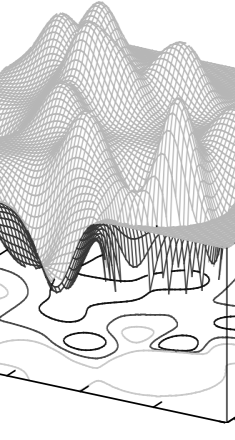
\includegraphics[height=7cm]{classPicture2-bw}
    }{\center

      \textbf{\fontsize{17}{20}\selectfont \course}

      ~

      %Lecture
      \topic\\

      \vspace{1cm}

      {\tiny~\emph{\keywords}~\\}

      \vspace{1cm}

      Marc Toussaint
      
      University of Stuttgart

      Summer 2019

      ~

    }
  }
}

\newcommand{\slide}[2]{
  \slidefont
  \incpage\begin{frame}
  \addcontentsline{toc}{section}{#1}
  \vfill
  {\headerfont #1} \vspace*{-2ex}
  \begin{itemize}\item[]~\\
    #2
  \end{itemize}
  \vfill
  \end{frame}
}

\newenvironment{slidecore}[1]{
  \slidefont\incpage
  \addcontentsline{toc}{section}{#1}
  \vfill
  {\headerfont #1} \vspace*{-2ex}
  \begin{itemize}\item[]~\\
}{
  \end{itemize}
  \vfill
}


\providecommand{\key}[1]{
  \addtocounter{mypage}{1}
% \immediate\write\keyfile{#1}
  \addtocontents{toc}{\hyperref[key:#1]{#1 (\arabic{mypage})}}
%  \phantomsection\label{key:#1}
%  \index{#1@{\hyperref[key:#1]{#1 (\arabic{mysec}:\arabic{mypage})}}|phantom}
  \addtocounter{mypage}{-1}
}

\providecommand{\course}{}

\providecommand{\subtopic}{}

\providecommand{\sublecture}[2]{
  \renewcommand{\subtopic}{#1}
  \slide{#1}{#2}
}

\providecommand{\story}[1]{
~

Motivation: {\tiny #1}\clearpage
}

\newenvironment{items}[1][9]{
\par\setlength{\unitlength}{1pt}\fontsize{#1}{#1}\linespread{1.2}\selectfont
\begin{list}{--}{\leftmargin4ex \rightmargin0ex \labelsep1ex \labelwidth2ex
\topsep0pt \parsep0ex \itemsep3pt}
}{
\end{list}
}

\providecommand{\slidesfoot}{
  \end{document}
}


  \slideshead
}

\providecommand{\exercises}{
  \newcommand{\exerciseshead}{
  \documentclass[10pt,fleqn]{article}
  \stdpackages

  \definecolor{bluecol}{rgb}{0,0,.5}
  \definecolor{greencol}{rgb}{0,.4,0}
  \definecolor{shadecolor}{gray}{0.9}
  \usepackage[
    %    pdftex%,
    %%    letterpaper,
    %    bookmarks,
    %    bookmarksnumbered,
    colorlinks,
    urlcolor=bluecol,
    citecolor=black,
    linkcolor=bluecol,
    %    pagecolor=bluecol,
    pdfborder={0 0 0},
    %pdfborderstyle={/S/U/W 1},
    %%    backref,     %link from bibliography back to sections
    %%    pagebackref, %link from bibliography back to pages
    %%    pdfstartview=FitH, %fitwidth instead of fit window
    pdfpagemode=UseNone, %UseOutlines, %bookmarks are displayed by acrobat
    pdftitle={\course},
    pdfauthor={Marc Toussaint},
    pdfkeywords={}
  ]{hyperref}
  \DeclareGraphicsExtensions{.pdf,.png,.jpg,.eps}

  \renewcommand{\r}{\varrho}
  \renewcommand{\l}{\lambda}
  \renewcommand{\L}{\Lambda}
  \renewcommand{\b}{\beta}
  \renewcommand{\d}{\delta}
  \renewcommand{\k}{\kappa}
  \renewcommand{\t}{\theta}
  \renewcommand{\O}{\Omega}
  \renewcommand{\o}{\omega}
  \renewcommand{\SS}{{\cal S}}
  \renewcommand{\=}{\!=\!}
  %\renewcommand{\boldsymbol}{}
  %\renewcommand{\Chapter}{\chapter}
  %\renewcommand{\Subsection}{\subsection}

  \renewcommand{\baselinestretch}{1.1}
  \geometry{a4paper,headsep=7mm,hdivide={15mm,*,15mm},vdivide={20mm,*,15mm}}

  \fancyhead[L]{\thetitle, \textit{Marc Toussaint}---\today}
  \fancyhead[R]{\thepage}
  \fancyhead[C]{}
  \fancyfoot{}
  \pagestyle{fancy}

  \parindent 0pt
  \parskip 0.5ex

  \newcommand{\codefont}{\helvetica{8}{1.2}{m}{n}}

  \input{../shared/macros}

  \DefineShortVerb{\@}

  \newcounter{solutions}
  \setcounter{solutions}{1}
  \newenvironment{solution}{
    \small
    \begin{shaded}
  }{
    \end{shaded}
  }
  
  \renewcommand{\hat}{\widehat}
  \newcommand{\bbg}{{\bar{\bar g}}}
  \graphicspath{{pics/}{../shared/pics/}}

  \renewcommand{\labelenumi}{{\alph{enumi})}}

  %%%%%%%%%%%%%%%%%%%%%%%%%%%%%%%%%%%%%%%%%%%%%%%%%%%%%%%%%%%%%%%%%%%%%%%%%%%%%%%%


  \mytitle{\course\\Exercise \exnum}
  \myauthor{Marc Toussaint\\ TAs: Janik Hager, Philipp Kratzer\\\small\addressUSTT}
  
  
  \begin{document}
  \onecolumn
  \maketitle
}

\newcommand{\exsection}[1]{\section{#1}}

\newcommand{\exerfoot}{
  \end{document}
}

\newenvironment{items}[1][9]{
  \par\setlength{\unitlength}{1pt}\fontsize{#1}{#1}\linespread{1.2}\selectfont
  \begin{list}{--}{\leftmargin4ex \rightmargin0ex \labelsep1ex \labelwidth2ex
      \topsep0pt \parsep0ex \itemsep3pt}
}{
  \end{list}
}

  \exerciseshead
}

\providecommand{\script}{
  \newcommand{\scripthead}{
  \documentclass[9pt,twoside]{article}
  \stdpackages

  \usepackage{palatino}
  \usepackage[envcountsect]{beamerarticle}
  \usepackage{makeidx}
  \makeindex

  \definecolor{bluecol}{rgb}{0,0,.5}
  \definecolor{greencol}{rgb}{0,.4,0}
  \definecolor{shadecolor}{gray}{0.9}
  \usepackage[
    %    pdftex%,
    %%    letterpaper,
    %bookmarks,
    bookmarksnumbered,
    colorlinks,
    urlcolor=bluecol,
    citecolor=black,
    linkcolor=bluecol,
    %    pagecolor=bluecol,
    pdfborder={0 0 0},
    %pdfborderstyle={/S/U/W 1},
    %%    backref,     %link from bibliography back to sections
    %%    pagebackref, %link from bibliography back to pages
    %%    pdfstartview=FitH, %fitwidth instead of fit window
    pdfpagemode=UseOutlines, %bookmarks are displayed by acrobat
    pdftitle={\course},
    pdfauthor={Marc Toussaint},
    pdfkeywords={}
  ]{hyperref}
  \DeclareGraphicsExtensions{.pdf,.png,.jpg,.eps}

  \usepackage{multimedia}
  %\setbeamercolor{background canvas}{bg=}

  \renewcommand{\r}{\varrho}
  \renewcommand{\l}{\lambda}
  \renewcommand{\L}{\Lambda}
  \renewcommand{\b}{\beta}
  \renewcommand{\d}{\delta}
  \renewcommand{\k}{\kappa}
  \renewcommand{\t}{\theta}
  \renewcommand{\O}{\Omega}
  \renewcommand{\o}{\omega}
  \renewcommand{\SS}{{\cal S}}
  \renewcommand{\=}{\!=\!}
  %\renewcommand{\boldsymbol}{}
  %\renewcommand{\Chapter}{\chapter}
  %\renewcommand{\Subsection}{\subsection}

  \renewcommand{\baselinestretch}{1.0}
  \geometry{a5paper,headsep=6mm,hdivide={10mm,*,10mm},vdivide={13mm,*,7mm}}

  \fancyhead[OL,ER]{\course, \textit{Marc Toussaint}}
  \fancyhead[OR,EL]{\thepage}
  \fancyhead[C]{}
  \fancyfoot{}
  \pagestyle{fancy}

%  \setcounter{tocdepth}{3}
  \setcounter{tocdepth}{2}

   \columnsep 6ex
  %  \renewcommand{\familydefault}{\sfdefault}
  \newcommand{\headerfont}{\large}%helvetica{12}{1}{b}{n}}
  \newcommand{\slidefont} {}%\helvetica{9}{1.3}{m}{n}}
  \newcommand{\storyfont} {}
  %  \renewcommand{\small}   {\helvetica{8}{1.2}{m}{n}}
  \renewcommand{\tiny}    {\footnotesize}%helvetica{7}{1.1}{m}{n}}
  \newcommand{\codefont}{\fontsize{6}{6}\selectfont}%helvetica{8}{1.2}{m}{n}}

  \input{../shared/macros}

  \DefineShortVerb{\@}

  \newcounter{solutions}
  \setcounter{solutions}{1}
  \renewenvironment{solution}{
    \small
    \begin{shaded}
  }{
    \end{shaded}
  }

  \graphicspath{{pics/}{../shared/pics/}}

%%%%%%%%%%%%%%%%%%%%%%%%%%%%%%%%%%%%%%%%%%%%%%%%%%%%%%%%%%%%%%%%%%%%%%%%%%%%%%%%

  \mytitle{\course\\Lecture Script}
  \myauthor{Marc Toussaint}

  \begin{document}

  %% \vspace*{2cm}

  \maketitle
  %\anchor{100,10}{\includegraphics[width=4cm]{optim}}

%  \vspace*{1cm}

  \emph{This is a direct concatenation and reformatting of all lecture
    slides and exercises from the \emph{Machine Learning} course (summer
    term 2019, U Stuttgart), including indexing to help
    prepare for exams.}

  \emph{Double-starred** sections and slides are not relevant for the exam.}

  {\tableofcontents}
}

%%%%%%%%%%%%%%%%%%%%%%%%%%%%%%%%%%%%%%%%%%%%%%%%%%%%%%%%%%%%%%%%%%%%%%%%%%%%%%%%

%% \renewcommand{\keywords}{}
%% \newcommand{\topic}{}
%% \renewcommand{\mypause}{}

  \newcounter{mypage}
  \setcounter{mypage}{0}
  \newcounter{mysec}
  \setcounter{mysec}{0}
  \newcommand{\incpage}{\addtocounter{mypage}{1}}
  \newcommand{\incsec} {\addtocounter{mysec}{1}}

\newcommand{\beginTocMinipage}{
  \addtocontents{toc}{\smallskip\noindent\hspace*{.036\columnwidth}}
  \addtocontents{toc}{\protect\begin{minipage}{.914\columnwidth}\small}
}
\newcommand{\closeTocMinipage}{
  \addtocontents{toc}{\protect\end{minipage}}
  \addtocontents{toc}{}
  \addtocontents{toc}{\medskip}
}

\renewcommand{\slides}[1][]{
  \clearpage
  \incsec
  \section{\topic}
  {\small #1}
  \beginTocMinipage
  \setcounter{mypage}{0}
  \smallskip\nopagebreak\hrule\medskip
}

\newcommand{\slidesfoot}{
  \closeTocMinipage
  \bigskip
}

\newcommand{\sublecture}[2]{
  \pagebreak[3]
  \incpage
  \closeTocMinipage
  \subsection{#1}
  {\storyfont #2}
  \beginTocMinipage
  {\hfill\tiny \textsf{\arabic{mysec}:\arabic{mypage}}}\nopagebreak%
  \smallskip\nopagebreak\hrule
}

\newcommand{\key}[1]{
  \pagebreak[2]
  \addtocounter{mypage}{1}
  \addtocontents{toc}{\hyperref[key:#1]{#1 (\arabic{mysec}:\arabic{mypage})}}
  \phantomsection\label{key:#1}
  \index{#1@{\hyperref[key:#1]{#1 (\arabic{mysec}:\arabic{mypage})}}|phantom}
  \addtocounter{mypage}{-1}
}

\newenvironment{slidecore}[1]{
  \incpage
  \subsubsection*{#1}%{\headerfont\noindent\textbf{#1}\\}%
  \vspace{-6ex}%
  \begin{list}{$\bullet$}{\leftmargin4ex \rightmargin0ex \labelsep1ex
    \labelwidth2ex \partopsep0ex \topsep0ex \parsep.5ex \parskip0ex \itemsep0pt}\item[]~\\\nopagebreak%
}{
  \end{list}\nopagebreak%
  {\hfill\tiny \textsf{\arabic{mysec}:\arabic{mypage}}}\nopagebreak%
  \smallskip\nopagebreak\hrule
}

\newcommand{\slide}[2]{
  \begin{slidecore}{#1}
    #2
  \end{slidecore}
}

\newcommand{\exsection}[1]{
  \subsubsection{#1}
}

\renewcommand{\exercises}{
  \subsection{Exercise \exnum}
}

\newcommand{\exerfoot}{
  \bigskip
}

\newcommand{\story}[1]{
  \subsection*{Motivation \& Outline}
  \addtocontents{toc}{\hyperref[mot\arabic{mysec}]{Motivation \& Outline}}
  \phantomsection\label{mot\arabic{mysec}}
  {\storyfont\sf #1}
  \medskip\nopagebreak\hrule
}

\newcounter{savedsection}
\newcommand{\subappendix}{\setcounter{savedsection}{\arabic{section}}\appendix}
\newcommand{\noappendix}{
  \setcounter{section}{\arabic{savedsection}}% restore section number
  \setcounter{subsection}{0}% reset section counter
%  \gdef\@chapapp{\sectionname}% reset section name
  \renewcommand{\thesection}{\arabic{section}}% make section numbers arabic
}

\newenvironment{items}[1][9]{
\par\setlength{\unitlength}{1pt}\fontsize{#1}{#1}\linespread{1.2}\selectfont
\begin{list}{--}{\leftmargin4ex \rightmargin0ex \labelsep1ex \labelwidth2ex
\topsep0pt \parsep0ex \itemsep3pt}
}{
\end{list}
}

  \scripthead
}

\providecommand{\course}{NO COURSE}
\providecommand{\topic}{NO TOPIC}
\providecommand{\keywords}{NO KEYWORDS}
\providecommand{\exnum}{NO NUMBER}


\providecommand{\stdpackages}{
  \usepackage{amsmath}
  \usepackage{amssymb}
  \usepackage{amsfonts}
  \allowdisplaybreaks
  \usepackage{amsthm}
  \usepackage{eucal}
  \usepackage{graphicx}
  \usepackage{color}
  \usepackage{geometry}
  \usepackage{framed}
%  \usecolor{xcolor}
  \definecolor{shadecolor}{gray}{0.9}
  \setlength{\FrameSep}{3pt}
  \usepackage{fancyvrb}
  \fvset{numbers=left,xleftmargin=5ex}

  \usepackage{multicol} 
  \usepackage{fancyhdr}
}

\providecommand{\addressUSTT}{
  Machine~Learning~\&~Robotics~lab, U~Stuttgart\\\small
  Universit{\"a}tsstra{\ss}e 38, 70569~Stuttgart, Germany
}


\renewcommand{\course}{Robotics}
\renewcommand{\coursepicture}{roboticsLecture}
\renewcommand{\coursedate}{Winter 2014}
\renewcommand{\topic}{Dynamics}

\slides

%%%%%%%%%%%%%%%%%%%%%%%%%%%%%%%%%%%%%%%%%%%%%%%%%%%%%%%%%%%%%%%%%%%%%%%%%%%%%%%%

\key{Dynamic vs. non-dynamic robots}
\slide{}{

\hspace*{-12mm}\begin{tabular}{p{.45\columnwidth}@{\qquad}|@{\qquad}p{.45\columnwidth}}
\cen{\large\textbf{Kinematic}} & \cen{\large\textbf{Dynamic}} \\[2ex]
 instantly change joint velocities $\dot q$:
&
 instantly change joint torques $u$:\\
\cen{$\d q_t \overset{!}= J^\sharp~ (y^* - \phi(q_t))$}
&
\cen{$u \overset{!}=$ ?} \\[2ex]

accounts for kinematic coupling of joints but
\textbf{ignores inertia, forces, torques}
&
accounts for dynamic coupling of joints and full
Newtonian physics\\[4ex]

gears, \textbf{stiff}, all of industrial robots\newline
\mov{\show[.15]{kukaStandardRobot.jpg}}{10-RoboticsLecture/11-Honda-All-New-ASIMO-hopping.mp4}
%\show[.9]{11-Honda-All-New-ASIMO-hopping2}
&
future robots, \textbf{compliant}, few research robots\newline
\show[.25]{barrett}

\end{tabular}

}

%%%%%%%%%%%%%%%%%%%%%%%%%%%%%%%%%%%%%%%%%%%%%%%%%%%%%%%%%%%%%%%%%%%%%%%%%%%%%%%%

\slide{When velocities cannot be changed/set arbitrarily}{

\item Examples:
\begin{items}
\item An air plane flying: You cannot command it to hold still in the
   air, or to move straight up.

\item A car: you cannot command it to move side-wards.

\item Your arm: you cannot command it to throw a ball with arbitrary
   speed (force limits).

\item A \emph{torque controlled} robot: You cannot command it to
   instantly change velocity (infinite acceleration/torque).
\end{items}

~

\item What all examples have in comment:
\begin{items}
\item One can set \textbf{controls} $u_t$ (air plane's control stick,
car's steering wheel, your muscles activations, torque/voltage/current
send to a robot's motors)

\item But these controls only indirectly influence the \textbf{dynamics of state}
\color{red}\Large\vspace*{-1ex}  $$x_{t\po} = f(x_t,u_t)$$
\end{items}
}

%%%%%%%%%%%%%%%%%%%%%%%%%%%%%%%%%%%%%%%%%%%%%%%%%%%%%%%%%%%%%%%%%%%%%%%%%%%%%%%%
\key{Definition of a dynamics equation}
\slide{Dynamics}{

\item The {dynamics} of a system describes how the controls
$u_t$ influence the change-of-state of the system

\eqbox{ $x_{t\po} = f(x_t,u_t)$ }

~

\begin{items}
\item The notation $x_t$ refers to the \emph{dynamic state} of the
   system: e.g., joint positions \emph{and velocities} $x_t =
   (q_t,\dot q_t)$.

\item $f$ is an arbitrary function, often smooth
\end{items}


}

%%%%%%%%%%%%%%%%%%%%%%%%%%%%%%%%%%%%%%%%%%%%%%%%%%%%%%%%%%%%%%%%%%%%%%%%%%%%%%%%

\slide{Outline}{

\item We start by discussing a \textbf{1D point mass} for 3 reasons:
\begin{items}
\item The most basic force-controlled system with inertia
\item We can introduce and understand \textbf{PID control}
\item The behavior of a point mass under PID control is
a \emph{reference} that we can also follow with arbitrary dynamic
robots (if the dynamics are known)
\end{items}

~

\item We discuss computing the dynamics of general robotic systems
\begin{items}
\item Euler-Lagrange equations
\item Euler-Newton method
\end{items}

\item We derive the dynamic equivalent of inverse kinematics:
\begin{items}
\item operational space control
\end{items}

}

%%%%%%%%%%%%%%%%%%%%%%%%%%%%%%%%%%%%%%%%%%%%%%%%%%%%%%%%%%%%%%%%%%%%%%%%%%%%%%%%

\sublecture{PID and a 1D point mass}

%%%%%%%%%%%%%%%%%%%%%%%%%%%%%%%%%%%%%%%%%%%%%%%%%%%%%%%%%%%%%%%%%%%%%%%%%%%%%%%%

\key{1D point mass}
\slide{The dynamics of a 1D point mass}{

\item Start with simplest possible example: 1D point mass

(no gravity, no friction, just a single mass)

~

\cen{\includegraphics[width=5cm]{mass-1}}

\item The {state} $x(t) = (q(t),\dot q(t))$ is described by:
\begin{items}
\item position $q(t) \in \RRR$
\item velocity $\dot q(t) \in \RRR$
\end{items}

~

\item The {controls} $u(t)$ is the force we apply on the mass point

~

\item The {system dynamics} is:
\begin{align*}
\ddot q(t) = u(t)/m
\end{align*}

}

%%%%%%%%%%%%%%%%%%%%%%%%%%%%%%%%%%%%%%%%%%%%%%%%%%%%%%%%%%%%%%%%%%%%%%%%%%%%%%%%
\key{P gain}
\slide{1D point mass -- proportional feedback}{

\item Assume current position is $q$.

The goal is to move it to the position $q^*$.

~

What can we do?

~\mypause

\item \textbf{\color{red}Idea 1:}

\emph{``Always pull the mass towards the goal $q^*$:''}
\begin{align*}
u = K_p~ (q^* - q)
\end{align*}

\cen{\includegraphics[width=5cm]{mass-2}}

}

%%%%%%%%%%%%%%%%%%%%%%%%%%%%%%%%%%%%%%%%%%%%%%%%%%%%%%%%%%%%%%%%%%%%%%%%%%%%%%%%
\slide{1D point mass -- proportional feedback}{

\item What's the effect of this control law?
\begin{align*}
m~ \ddot q
 & = u = K_p~ (q^* - q)
\end{align*}

$q = q(t)$ is a function of time, this is a second order differential equation

\mypause

\item Solution: ~ {\color{blue}assume $q(t) = a + b e^{\o t}$}

(a ``non-imaginary'' alternative would be $q(t) = a + b~ \e^{-\l
t}~ \cos(\o t)$)
\mypause%
\begin{align*}
&m~ b~ \o^2~ e^{\o t}
 = K_p~ q^* - K_p~ a - K_p~ b~ e^{\o t} \\
&(m~ b~ \o^2 + K_p~ b)~ e^{\o t}
  = K_p~ (q^* - a) \\
&\To
  (m~ b~ \o^2 + K_p~ b) = 0 ~\wedge~ (q^*-a) = 0 \\
& \To ~ \o = i \sqrt{K_p/m} \\
&q(t)
  = q^* + b~ e^{i \sqrt{K_p/m}~ t}
\end{align*}

This is an oscillation around $q^*$ with amplitude $b=q(0)-q^*$ and
frequency $\sqrt{K_p/m}$!

}

%%%%%%%%%%%%%%%%%%%%%%%%%%%%%%%%%%%%%%%%%%%%%%%%%%%%%%%%%%%%%%%%%%%%%%%%%%%%%%%%
\slide{1D point mass -- proportional feedback}{

\begin{align*}
&m~ \ddot q
  = u = K_p~ (q^* - q) \\
&q(t)
  = q^* + b~ e^{i \sqrt{K_p/m}~ t}
\end{align*}

Oscillation around $q^*$ with amplitude $b=q(0)-q^*$ and
frequency $\sqrt{K_p/m}$

~

\cen{\includegraphics[angle=-90,width=8cm]{cosine}}

%set terminal postscript
%set output 'cosine.eps'
%set size 1.0,.5
%plot[0:15][-1.1:1.1] cos(x) lw 3

}


%%%%%%%%%%%%%%%%%%%%%%%%%%%%%%%%%%%%%%%%%%%%%%%%%%%%%%%%%%%%%%%%%%%%%%%%%%%%%%%%
\key{D gain}
\slide{1D point mass -- derivative feedback}{

\item \textbf{\color{red}Idea 2}

\emph{``Pull less, when we're heading the right direction already:''}

\emph{``Damp the system:''}
\begin{align*}
u = K_p (q^* - q) + K_d (\dot q^* - \dot q)
\end{align*}

$\dot q^*$ is a desired goal velocity

For simplicity we set $\dot q^* = 0$ in the following.

~

~

\cen{\includegraphics[width=5cm]{mass-3}}

}

%%%%%%%%%%%%%%%%%%%%%%%%%%%%%%%%%%%%%%%%%%%%%%%%%%%%%%%%%%%%%%%%%%%%%%%%%%%%%%%%
\slide{1D point mass -- derivative feedback}{

\item What's the effect of this control law?
\begin{align*}
m \ddot q
 & = u
   = K_p (q^* - q) + K_d (0 - \dot q)
\end{align*}

\item Solution: ~ {\color{blue}again assume $q(t) = a + b e^{\o t}$}
\begin{align*}
&m~ b~ \o^2~ e^{\o t}
 = K_p~ q^* - K_p~ a - K_p~ b~ e^{\o t} - K_d~ b~ \o e^{\o t}\\
&(m~ b~ \o^2 + K_d~ b~ \o + K_p~ b)~ e^{\o t}
 = K_p~ (q^* - a) \\
&\To (m~ \o^2 + K_d~ \o + K_p) = 0 ~\wedge~ (q^*-a) = 0 \\
&\To \o = \frac{-K_d \pm \sqrt{K_d^2 - 4 m K_p}}{2m} \\
&q(t)
 = q^* + b~ e^{\o~ t}
\end{align*}

The term $-\frac{K_d}{2m}$ in $\o$ is real ~ $\oto$ ~ exponential decay (damping)

}

%%%%%%%%%%%%%%%%%%%%%%%%%%%%%%%%%%%%%%%%%%%%%%%%%%%%%%%%%%%%%%%%%%%%%%%%%%%%%%%%
\slide{1D point mass -- derivative feedback}{

$$q(t)
 = q^* + b~ e^{\o~ t}
\comma \o = \frac{-K_d \pm \sqrt{K_d^2 - 4 m K_p}}{2m}$$

~

\item Effect of the second term $\sqrt{K_d^2 - 4 m K_p}/2m$ in $\o$:

~

\begin{tabular}{c@{\quad$\To$\quad}p{.7\columnwidth}}
$K_d^2 < 4 m K_p$
&
$\o$ has imaginary part\newline
oscillating with frequency $\sqrt{K_p/m - K_d^2/4m^2}$\newline
$q(t) = q^* + b e^{-K_d/2m~ t}~ e^{i \sqrt{K_p/m - K_d^2/4m^2}~ t}$
\\
$K_d^2 > 4 m K_p$
&
$\o$ real\newline
strongly damped
\\
$K_d^2 = 4 m K_p$
&
second term zero\newline
only exponential decay
\end{tabular}

}


%%%%%%%%%%%%%%%%%%%%%%%%%%%%%%%%%%%%%%%%%%%%%%%%%%%%%%%%%%%%%%%%%%%%%%%%%%%%%%%%
\key{oscillatory-damped, critically damped, over-damped}
\slide{1D point mass -- derivative feedback}{

\show[.9]{dampenings}
\hfill{\tiny illustration from O. Brock's lecture}

%% $\xi^2 = \frac{K_d^2}{4m K_p}$

%% $\xi = \frac{K_d}{4\sqrt{m K_p}}$

%% $\xi <1$ $\To$


}

%%%%%%%%%%%%%%%%%%%%%%%%%%%%%%%%%%%%%%%%%%%%%%%%%%%%%%%%%%%%%%%%%%%%%%%%%%%%%%%%
\key{Damping ration, wave length}
\slide{1D point mass -- derivative feedback}{

Alternative parameterization:

Instead of the \emph{gains} $K_p$ and $K_d$ it is sometimes more
intuitive to set the

~

\item wave length $\l = \frac{1}{\o_0} = \frac{1}{\sqrt{K_p/m}} \comma K_p = m/\l^2$

~

\item damping ratio $\xi
 = \frac{K_d}{\sqrt{4m K_p}}
 = \frac{\l K_d}{2m}
 \comma K_d = 2m\xi/\l$

~

$\xi > 1$: over-damped

$\xi = 1$: critically dampled

$\xi < 1$: oscillatory-damped

$$q(t) = q^* + b e^{-\xi~ t/\l}~ e^{i \sqrt{1-\xi^2}~ t/\l}$$

}

%%%%%%%%%%%%%%%%%%%%%%%%%%%%%%%%%%%%%%%%%%%%%%%%%%%%%%%%%%%%%%%%%%%%%%%%%%%%%%%%
\key{I gain}
\slide{1D point mass -- integral feedback}{

\item \textbf{\color{red}Idea 3}

\emph{``Pull if the position error accumulated large in the past:''}

\begin{align*}
u = K_p (q^* - q) + K_d (\dot q^* - \dot q) + K_i \int_{s=0}^t (q^*(s) - q(s))~ ds
\end{align*}

~\tiny

\item This is not a linear ODE w.r.t.\ $x=(q,\dot q)$.

However, when we extend the state to $x=(q,\dot q,e)$ we have the ODE
\begin{align*}
\dot q
 &= \dot q \\
\ddot q
 &= u/m = K_p/m (q^* - q) + K_d/m (\dot q^* - \dot q) + K_i/m~ e \\
\dot e
 &= q^* - q
\end{align*}

(no explicit discussion here)

}

%%%%%%%%%%%%%%%%%%%%%%%%%%%%%%%%%%%%%%%%%%%%%%%%%%%%%%%%%%%%%%%%%%%%%%%%%%%%%%%%
\key{PID control}
\slide{1D point mass -- PID control}{

\begin{align*}
u = K_p (q^* - q) + K_d (\dot q^* - \dot q) + K_i \int_{s=0}^t (q^* - q(s))~ ds
\end{align*}

~

\item\textbf{PID control}

-- Proportional Control (``Position Control'')

~~ $u \propto K_p (q^* - q)$

~

-- Derivative Control (``Damping'')

~~ $u \propto K_d (\dot q^* - \dot q)$  ~~ ($\dot x^*=0$ $\to$ damping)

~

-- Integral Control (``Steady State Error'')

~~ $u \propto K_i \int_{s=0}^t (q^*(s) - q(s))~ ds$

}


%%%%%%%%%%%%%%%%%%%%%%%%%%%%%%%%%%%%%%%%%%%%%%%%%%%%%%%%%%%%%%%%%%%%%%%%%%%%%%%%

\slide{Controlling a 1D point mass -- lessons learnt}{

\item Proportional and derivative feedback (PD control) are like
adding a spring and damper to the point mass

~

\item PD control is a \emph{linear control law}

 $$(q,\dot q) \mapsto u = K_p (q^* - q) + K_d (\dot q^* - \dot
 q)$$

(linear in the \emph{dynamic system state} $x=(q,\dot q)$)

~

\item With such linear control laws we can design 
approach trajectories (by tuning the gains)

-- but no optimality principle behind such motions

}

%%%%%%%%%%%%%%%%%%%%%%%%%%%%%%%%%%%%%%%%%%%%%%%%%%%%%%%%%%%%%%%%%%%%%%%%%%%%%%%%
\sublecture{Dynamics of mechanical systems}

%%%%%%%%%%%%%%%%%%%%%%%%%%%%%%%%%%%%%%%%%%%%%%%%%%%%%%%%%%%%%%%%%%%%%%%%%%%%%%%%
\slide{Two ways to derive dynamics equations for mechanical systems}{

\item The Euler-Lagrange equation, $L=L(t, q(t), \dot q(t))$,
$$ \frac{d}{dt} \frac{\del L}{\del \dot q} - \frac{\del L}{\del q} = u $$
{\small Used when you want to derive analytic equations of
motion (``on paper'')}

~

\item The Newton-Euler recursion ~ (and related algorithms)
$$f_i = m \dot v_i \comma u_i = I_i \dot w + w\times I w$$ {\small
Algorithms that ``propagate'' forces through a kinematic tree and
numerically compute the \emph{inverse} dynamics $u=\text{NE}(q,\dot
q,\ddot q)$ or \emph{forward} dynamics $\ddot q = f(q,\dot q,u)$.

} 

}

%%%%%%%%%%%%%%%%%%%%%%%%%%%%%%%%%%%%%%%%%%%%%%%%%%%%%%%%%%%%%%%%%%%%%%%%%%%%%%%%
\key{Euler-Lagrange equation}
\slide{The Euler-Lagrange equation}{

$$\frac{d}{dt} \frac{\del L}{\del \dot q} - \frac{\del L}{\del q} = u$$

\item $L(q,\dot q)$ is called \textbf{Lagrangian} and defined as
$$L = T - U$$
where $T$=kinetic energy and $U$=potential energy.

\item $q$ is called generalized coordinate -- any coordinates such that
 $(q,\dot q)$ describes the state of the system. Joint angles in our
 case.

\item $u$ are external forces

}

%%%%%%%%%%%%%%%%%%%%%%%%%%%%%%%%%%%%%%%%%%%%%%%%%%%%%%%%%%%%%%%%%%%%%%%%%%%%%%%%
\key{Pendulum example for Euler-Lagrange}
\slide{Example: A pendulum}{

\shows[1]{pendulum}

\item Generalized coordinates: angle $q=(\t)$

\item Kinematics:
\begin{items}
\item velocity of the mass: $v = (l\dot\t\cos\t, 0, l\dot\t\sin\t)$
\item angular velocity of the mass: $w = (0, -\dot\t, 0)$
\end{items}

\item Energies:
$$T=\half m v^2 + \half w^\T I w = \half (ml^2 + I_2)\dot\t^2\comma U
= - m g l\cos\t$$

\item Euler-Lagrange equation:
\begin{align*}
u
&=\frac{d}{dt} \frac{\del L}{\del \dot q} - \frac{\del L}{\del q} \\
&=\frac{d}{dt} (ml^2 + I_2)\dot\t + m g l\sin\t 
 = (ml^2 + I_2)\ddot\t + m g l\sin\t
\end{align*}

}


%%%%%%%%%%%%%%%%%%%%%%%%%%%%%%%%%%%%%%%%%%%%%%%%%%%%%%%%%%%%%%%%%%%%%%%%%%%%%%%%
\key{General structure of Euler-Lagrange}
\slide{The Euler-Lagrange equation}{

\small

\item How is this typically done?

\item \textbf{First}, describe the \emph{kinematics and Jacobians} for
every link $i$:
$$(q,\dot q)\mapsto \{ T_{W\to i}(q), v_i, w_i \}$$

{\tiny Recall $T_{W\to i}(q)
 = T_{W\to A}~ {\color{red}T_{A\to A'}(q)}~
   T_{A'\to B}~ {\color{red}T_{B\to B'}(q)}~
   \cdots$

Further, we know that a link's velocity $v_i=J_i \dot q$ can be
described via its position Jacobian.

Similarly we can describe the link's \emph{angular velocity} $w_i = J^w_i \dot q$ as linear in $\dot q$.

}

\item \textbf{Second}, formulate the kinetic energy
$$T = \sum_i \half m_i v_i^2 + \half w_i^\T I_i w_i
= \sum_i \half \dot q^\T M_i \dot q
\comma M_i = \mat{c}{J_i\\J^w_i}^\T \mat{cc}{m_i\Id_3 & 0 \\ 0 & I_i} \mat{c}{J_i\\J^w_i} $$
where $I_i = R_i \bar I_i R_i^\T$ and $\bar I_i$ the inertia tensor in
link coordinates

\item \textbf{Third}, formulate the potential energies (typically independent of $\dot q$)
$$U = g m_i \text{height}(i)$$

\item \textbf{Fourth}, compute the partial derivatives analytically to
get something like
\begin{align*}
\underbrace{u}_\text{control} = \frac{d}{dt} \frac{\del L}{\del \dot q} - \frac{\del L}{\del q} 
 = \underbrace{M}_\text{inertia} \ddot q + \underbrace{\dot M \dot q
 - \frac{\del T}{\del q}}_\text{Coriolis} + \underbrace{\frac{\del U}{\del q}}_\text{gravity}
\end{align*}
which relates accelerations $\ddot q$ to the forces

}

%%%%%%%%%%%%%%%%%%%%%%%%%%%%%%%%%%%%%%%%%%%%%%%%%%%%%%%%%%%%%%%%%%%%%%%%%%%%%%%%

%% \slide{Computing $M$ and $F$}{

%% \cen{$M(q)~ \ddot q + F(q,\dot q) = u$}

%% \item Recall:

%% We have an algorithm to compute all positions and
%% orientations given $q$:

%% $T_{W\to i}(q)
%%  = T_{W\to A}~ {\color{red}T_{A\to A'}(q)}~
%%    T_{A'\to B}~ {\color{red}T_{B\to B'}(q)}~
%%    T_{B'\to C}~ {\color{red}T_{C\to C'}(q)}~
%%    T_{C'\to i}$

%% ~\mypause

%% \item This can be extended easily to compute also:

%% -- linear velocities $v_i$

%% -- angular velocities $w_i$

%% -- linear accelerations $\dot v_i$

%% -- angular accelerations $\dot w_i$

%% for any link $i$ in the robot ~ (via forward propagation; see
%% geometry notes for details).

%% }

%%%%%%%%%%%%%%%%%%%%%%%%%%%%%%%%%%%%%%%%%%%%%%%%%%%%%%%%%%%%%%%%%%%%%%%%%%%%%%%%
\key{Newton-Euler recursion}
\slide{Newton-Euler recursion}{

\item An algorithm that computes the \emph{inverse dynamics}
$$u=\text{NE}(q,\dot q,\ddot q^*)$$ by recursively computing force
balance at each joint:
\begin{items}
\item \textbf{Newton's equation} ~ expresses the force acting at the center of mass for an accelerated body:
$$f_i = m \dot v_i$$

\item \textbf{Euler's equation} ~ expresses the torque (=control) acting on a
rigid body given an angular velocity and angular acceleration:
$$u_i = I_i \dot w + w\times I w$$
\end{items}

~

\item \textbf{Forward recursion:} ($\approx$ kinematics)

Compute (angular) velocities $(v_i, w_i)$ \emph{and} accelerations
$(\dot v_i,\dot w_i)$ for every link {\tiny(via forward propagation; see
geometry notes for details)}

~

\item \textbf{Backward recursion:}

For the leaf links, we now know the desired accelerations $q^*$ and can
compute the necessary joint torques. Recurse backward.

}

%%%%%%%%%%%%%%%%%%%%%%%%%%%%%%%%%%%%%%%%%%%%%%%%%%%%%%%%%%%%%%%%%%%%%%%%%%%%%%%%

\slide{Numeric algorithms for forward and inverse dynamics}{

\item \textbf{Newton-Euler recursion}:~ very fast ($O(n)$) method to compute
\emph{inverse} dynamics $$u=\text{NE}(q,\dot q,\ddot q^*)$$
{\tiny Note that we can use this algorithm to also compute
\begin{items}
\item gravity terms:~ $u = \text{NE}(q,0,0) = G(q)$ 
\item Coriolis terms:~ $u = \text{NE}(q,\dot q,0) = C(q,\dot q)~ \dot q + G(q)$
\item column of Intertia matrix:~ $u = \text{NE}(q,0,e_i) = M(q)~ e_i$
\end{items}
}

~

\item \textbf{Articulated-Body-Dynamics}:~ fast method ($O(n)$) to compute \emph{forward}
dynamics $\ddot q = f(q,\dot q,u)$

}

%%%%%%%%%%%%%%%%%%%%%%%%%%%%%%%%%%%%%%%%%%%%%%%%%%%%%%%%%%%%%%%%%%%%%%%%%%%%%%%%

\slide{Some last practical comments}{

\item \texttt{[demo]}

\item Use \emph{energy conservation} to measure dynamic of physical
simulation

\item Physical simulation engines (developed for games):
\begin{items}
\item ODE (Open Dynamics Engine)
\item Bullet (originally focussed on collision only)
\item Physx (Nvidia)
\end{items}

Differences of these engines to Lagrange, NE or ABD:
\begin{items}
\item Game engine can model much more: Contacts, tissues,
particles, fog, etc
\item (The way they model contacts looks ok but is somewhat fictional)
\item On kinematic trees, NE or ABD are much
more precise than game engines
\item Game engines do not provide \emph{inverse} dynamics, $u=\text{NE}(q,\dot
q,\ddot q)$
\end{items}

~

\item Proper modelling of contacts is really really hard

}

%%%%%%%%%%%%%%%%%%%%%%%%%%%%%%%%%%%%%%%%%%%%%%%%%%%%%%%%%%%%%%%%%%%%%%%%%%%%%%%%
\sublecture{Controlling a dynamic robot}

%%%%%%%%%%%%%%%%%%%%%%%%%%%%%%%%%%%%%%%%%%%%%%%%%%%%%%%%%%%%%%%%%%%%%%%%%%%%%%%%

\slide{}{

\item We previously learnt the effect of PID control on a 1D point
mass

~

\item Robots are not a 1D point mass
\begin{items}
\item Neither is each joint a 1D point mass
\item Applying separate PD control in each joint neglects force
coupling

(Poor solution: Apply very high gains separately in each joint $\oto$
make joints stiff, as with gears.)
\end{items}

~

\item However, knowing the robot dynamics we can transfer our
understanding of PID control of a point mass to general systems

}

%%%%%%%%%%%%%%%%%%%%%%%%%%%%%%%%%%%%%%%%%%%%%%%%%%%%%%%%%%%%%%%%%%%%%%%%%%%%%%%%
\key{General structure of robot dynamics}
\slide{General robot dynamics}{

\item Let $(q, \dot q)$ be the dynamic state and $u\in\RRR^n$ the
controls (typically joint torques in each
motor) of a robot

\item Robot dynamics can generally be written as:
$$
M(q)~ \ddot q + C(q,\dot q)~ \dot q + G(q) = u
$$
{\small\begin{tabular}{cp{.7\columnwidth}}
$M(q) \in \RRR^{n\times n}$
& is positive definite intertia matrix\newline (can be inverted $\to$
forward simulation of dynamics)
\\
$C(q,\dot q) \in \RRR^n$
& are the centripetal and coriolis forces
\\
$G(q) \in \RRR^n$
& are the gravitational forces
\\
$u$
& are the joint torques
\end{tabular}

}

(cf.\ to the Euler-Lagrange equation on slide 22)


\item We often write more compactly:

\eqbox{$M(q)~ \ddot q + F(q,\dot q) = u$}

}

%%%%%%%%%%%%%%%%%%%%%%%%%%%%%%%%%%%%%%%%%%%%%%%%%%%%%%%%%%%%%%%%%%%%%%%%%%%%%%%%
\key{Inverse and forward dynamics}
\slide{Controlling a general robot}{

\item From now on we just assume that we have algorithms to
efficiently compute $M(q)$ and $F(q,\dot q)$ for any $(q,\dot q)$

\item \textbf{Inverse dynamics:}~ If we know the desired $\ddot q^*$
for each joint, 
$$u = M(q)~ \ddot q^* + F(q,\dot q)$$
gives the necessary torques

\item \textbf{Forward dynamics:}~ If we know which torques $u$ we
apply, use
$$\ddot q^* = M(q)^\1 (u-F(q,\dot q))$$
to simulate the dynamics of the system (e.g., using Runge-Kutta)

}

%%%%%%%%%%%%%%%%%%%%%%%%%%%%%%%%%%%%%%%%%%%%%%%%%%%%%%%%%%%%%%%%%%%%%%%%%%%%%%%%
\key{Following a reference trajectory in joint space}
\slide{Following a reference trajectory in joint space}{

\item Where could we get the desired $\ddot q^*$ from?

Assume we have a nice smooth \textbf{reference trajectory}
$q_{0:T}^\text{ref}$ (generated with some motion profile or alike), we
can at each $t$ read off the desired acceleration as
$$\ddot q_t^\text{ref}
 := \frac{1}{\tau}[(q_{t\po}-q_t)/\tau - (q_t-q_{t\1})/\tau]
  = (q_{t\1} + q_{t\po} - 2q_t)/\tau^2$$

However, tiny errors in acceleration will accumulate greatly over
time! This is Instable!!

\mypause

\item Choose a desired acceleration $\ddot q_t^*$ that implies
a \emph{PD-like behavior around the reference trajectory}!

\eqbox{$\ddot q_t^* = \ddot q_t^\text{ref} + K_p(q_t^\text{ref} - q_t) + K_d(\dot q_t^\text{ref} - \dot q_t)$}

\small
This is a standard and very convenient heuristic to track a reference
trajectory when the robot dynamics are known: \emph{All joints will exactly
behave like a 1D point particle around the reference trajectory!}

}

%%%%%%%%%%%%%%%%%%%%%%%%%%%%%%%%%%%%%%%%%%%%%%%%%%%%%%%%%%%%%%%%%%%%%%%%%%%%%%%%

%% \slide{Dynamic reaching}{

%% \item How can we accelerate all joints \emph{to reach an
%% endeffector target $y^*$}?

%% -- 1D point mass $\to$ PD control can generate approach
%%    trajectories

%% -- How can we combine things?

%% \mypause

%% \emph{2 ways of thinking:}

%% \item \textbf{Joint space approach:}

%% 1) Compute target joint angles $q^*$ from $y^*$ using inverse
%% kinematics.

%% 2) Compute $u$ to ``mimick'' PD behavior in all
%% joints:

%% ~~ $\ddot q^* = K_p(q^* - q) + K_d(0 - \dot q)$

%% ~~ $u = M(q)~ \ddot q^* + F(q,\dot q)$

%% (better than separate PD controllers for each joint! cancels all
%% natural forces; behaves like an $n$-dimensional point mass)

%% \mypause

%% \item \textbf{Operational space approach:}

%% 1) Compute a desired
%% effector acceleration $\ddot y^*$ mimicking PD behavior.

%% 2) Translate this ``somehow'' to desired acceleration $\ddot q^*$:

%% $\ddot y^* = K_p(y^* - y) + K_d(0 - \dot y)$

%% $u = \text{function of }(\ddot y^*)$

%% }

%%%%%%%%%%%%%%%%%%%%%%%%%%%%%%%%%%%%%%%%%%%%%%%%%%%%%%%%%%%%%%%%%%%%%%%%%%%%%%%%
\key{Following a reference trajectory in task space}
\slide{Following a reference trajectory in task space}{

\item Recall the inverse kinematics problem:
\begin{items}
\item We know the desired step $\d y^*$ (or velocity $\dot y^*$) of the \emph{endeffector}.

\item Which step $\d q$ (or velocities $\dot q$) should we make in the
joints?
\end{items}

~

\item Equivalent dynamic problem:
\begin{items}
\item We know how the desired acceleration $\ddot y^*$ of
   the \emph{endeffector}.
\item What controls $u$ should we apply?
\end{items}

}

%%%%%%%%%%%%%%%%%%%%%%%%%%%%%%%%%%%%%%%%%%%%%%%%%%%%%%%%%%%%%%%%%%%%%%%%%%%%%%%%

%% \slide{Linear(ized) system and linear control}{

%% System state is given as $\bar q_t=\mat{c}{q_t\\ \dot q_t}$
%% \begin{align}
%% &P(q_{t\po} \| \dot q_t, q_t)
%%  = \NN(q_{t\po} \| q_t + u \dot q_{t\po}, W^\1) ~,\\
%% &P(\dot q_{t\po} \| \dot q_t, u_t)
%%  = \NN(\dot q_{t\po} \| \dot q_t + u M^\1(u_t+F), Q) ~,\\
%% %
%% &\mat{c}{q_{t\po}\\ \dot q_{t\po}}
%%  = \mat{c@{~}c}{1&u\\0&1}~ \mat{c}{q_t\\ \dot q_t} +
%%  \mat{c}{u^2\\u} M^\1 (u_t+F) + \xi \comma \<d\xi d\xi^\T\> = \mat{c@{~}c}{W^\1&0\\0&Q} \\
%% %
%% & A=\mat{c@{~}c}{1&u\\0&1}
%%   \comma B=\mat{c}{u^2 M^\1\\u M^\1}
%%   \comma a=\mat{c}{u^2 M^\1 F\\u M^\1 F}
%% \end{align}

%% }

%%%%%%%%%%%%%%%%%%%%%%%%%%%%%%%%%%%%%%%%%%%%%%%%%%%%%%%%%%%%%%%%%%%%%%%%%%%%%%%%
\key{Operational space control}
\slide{Operational space control}{

~

\item Inverse kinematics:
$$q^* = \argmin_q \norm{\phi(q) - y^*}^2_C + \norm{q-q_0}^2_W $$

~

\item Operational space control (one might call it ``Inverse task space dynamics''):
$$u^* = \argmin_u \norm{\ddot\phi(q) - \ddot y^*}^2_C + \norm{u}^2_H$$

\label{pageObjFunc}

}

%%%%%%%%%%%%%%%%%%%%%%%%%%%%%%%%%%%%%%%%%%%%%%%%%%%%%%%%%%%%%%%%%%%%%%%%%%%%%%%%



%% ~

%% \item what is actually $\dot y_{t\po}$ and $y_{t\po}$ depending on
%% $u$?

%% Euler integration:
%% \begin{align*}
%% \mat{c}{q_{t\po}\\ \dot q_{t\po}}
%%  = \mat{c}{q_t + \tau \dot q_t  \\
%%            \dot q_t + \tau  M^\1 (u-F)}
%%  = \mat{cc}{1&\tau\\0&1}~ \mat{c}{q_t\\ \dot q_t} +
%%     \mat{c}{0\\\tau} M^\1 (u-F)
%% \end{align*}

%% Leap frog integration:
%% \begin{align*}
%% \mat{c}{q_{t\po}\\ \dot q_{t\po}}
%%  = \mat{c}{q_t + \tau \dot q_t + \tau^2/2~ M^\1 (u-F)
%%            \dot q_t + \tau  M^\1 (u-F)}
%%   = \mat{cc}{1&\tau\\0&1}~ \mat{c}{q_t\\ \dot q_t} +
%%     \mat{c}{\tau^2/2\\\tau} M^\1 (u-F)
%% \end{align*}

%% }

%%%%%%%%%%%%%%%%%%%%%%%%%%%%%%%%%%%%%%%%%%%%%%%%%%%%%%%%%%%%%%%%%%%%%%%%%%%%%%%%
\slide{Operational space control}{

%% discrete time:
%% \begin{align*}
%% f(u)
%%  &= \norm{u}_{H} \\
%%  &+ \norm{\dot y^* - J \dot q_t - \tau J M^\1 (u-F)}_{D}
%%  &+ \norm{y^* - \phi(q_t) - \tau J \dot q_t - \tau^2/2~ J M^\1 (u-F)}_{C}
%% \end{align*}
%% (here we approximate $\dot J=0$!)

~

\item We can derive the optimum perfectly analogous to inverse
kinematics

{\small We identify the minimum of a locally squared potential, using
the local linearization (and approx. $\ddot J=0$)
$$
\ddot \phi(q)
  = \frac{d}{dt} \dot \phi(q)
  \approx \frac{d}{dt}(J\dot q+\dot J q)
  \approx J \ddot q + 2\dot J \dot q
  = J M^\1 (u-F) + 2\dot J \dot q
$$

}

We get
\begin{align*}
u^*
 &= T^\sharp (\ddot y^* - 2\dot J \dot q + T F)\\
% &= T^\sharp (\dot y^* - J \dot q_t + \tau T F)\\
 &\text{ with } T = J M^\1 \comma T^\sharp = (T^\T C T + H)^\1 T^\T C
\end{align*}
($C\to\infty ~\To~ T^\sharp = H^\1 T^\T (T H^\1 T^\T)^\1$)

}

%%%%%%%%%%%%%%%%%%%%%%%%%%%%%%%%%%%%%%%%%%%%%%%%%%%%%%%%%%%%%%%%%%%%%%%%%%%%%%%%

\slide{Controlling a robot -- operational space approach}{

\item Where could we get the desired $\ddot y^*$ from?

-- \textbf{Reference trajectory} $y_{0:T}^\text{ref}$ in operational space

-- \textbf{PD-like behavior} in each operational space:

\cen{$\ddot y_t^* = \ddot y_t^\text{ref} + K_p(y_t^\text{ref} - y_t) + K_d(\dot y_t^\text{ref} - \dot y_t)$}

~

\show[.8]{jointSpace-operationalSpace}
\hfill{\tiny illustration from O. Brock's lecture}

~

\item Operational space control: \emph{Let the system behave as if we could directly
``apply a 1D point mass behavior'' to the endeffector}


}


%%%%%%%%%%%%%%%%%%%%%%%%%%%%%%%%%%%%%%%%%%%%%%%%%%%%%%%%%%%%%%%%%%%%%%%%%%%%%%%%

%% \slide{Summary}{

%% \renewcommand{\arraystretch}{1.8}

%% \hspace*{-5mm}\begin{tabular}{|p{.27\columnwidth}|c|c|c|}
%% \hline
%% & State & Controls & Dynamics \\
%% %\hline
%% general notation
%% & $x$
%% & $u$
%% & $\dot x = f(x,u)$ \\
%% \hline
%% \hline
%% Kinematic control
%% & $x=q$
%% & $u=\dot q$
%% & $\dot q = u$ (can be \emph{set}) \\
%% \hline
%% 1D Point mass
%% & $x = \mat{c}{q \\ \dot q}$
%% & $u = \text{force}$
%% & $\dot x = \mat{c}{\dot q \\
%% u/m}$ \\
%% \hline
%% General dynamic\newline system
%% & $x = \mat{c}{q \\ \dot q}$
%% & $u = \text{torque}$
%% & $\dot x = \mat{c}{\dot q \\ M^\1(u-F)}$ \\
%% \hline
%% Car
%% & $q = \mat{c}{x \\ y \\ \t}$
%% & $u = \mat{c}{v \\ \varphi}$
%% & $\dot q = \mat{c}{v~ \cos \t \\ v~ \sin \t \\ (v/L)~ \tan \varphi }$\\
%% \hline
%% \end{tabular}

%% ~

%% Only kinematic control has $\dim(u)=\dim(x)$, all others $\dim(u)<\dim(x)$

%% }





%%%%%%%%%%%%%%%%%%%%%%%%%%%%%%%%%%%%%%%%%%%%%%%%%%%%%%%%%%%%%%%%%%%%%%%%%%%%%%%%


%% \slide{Analogies:~ motion rate and dynamic control}{


%% \small
%% \hspace*{-11mm}\begin{tabular}{|p{.19\columnwidth}|p{.26\columnwidth}|p{.5\columnwidth}|}
%% \hline
%% & motion rate control
%% & dynamic control \\
%% \hline
%% control interface
%% & can set \emph{velocities} $\dot q$ of servo motors
%% & can set \emph{torques} $u$ for each
%% joint  (or other \emph{control signals} $u$)\\
%% \hline
%% effect after a\newline time step $\tau$
%% & a step $\d q = \tau \dot q$ in joint angles
%% & a change $\d \dot q = \tau \ddot q$ in velocity \\
%% \hline
%% system\newline equation %$x_{t\po} = f(x_t,u)$
%% & $q_{t\po} = q_t + \tau \dot q$
%% & $M(q)~ \ddot q + F(q,\dot q) = u$ \newline
%%   $\mat{c}{q_{t\po}\\ \dot q_{t\po}}
%%   = \mat{c@{~}c}{1&\tau\\0&1}~ \mat{c}{q_t\\ \dot q_t} +
%%     \mat{c}{\tau^2/2\\\tau} M^\1 (u-F)$ \\
%% \hline
%% optimality: & & \\
%% 1) lazyness
%% & %$\norm{\dot q}_{W}^2$ \newline
%%   $\norm{q_{t\po} - q_t}_{W}^2$
%% & $\norm{u}_{H}^2$ \\
%% 2) task
%% & %$\norm{\dot y^* - J \dot q}_{C}^2$ \newline
%%   $\norm{\phi(q_{t\po}) - y^*}_{C}^2$
%% & $\norm{J M^\1 (u-F) + \dot J\dot q - \ddot y^*}_{C}^2$ \\
%% \hline
%% optimal solution
%% & %$\dot q = J^\sharp~ \dot y^*$ \newline
%%   $\d q = J^\sharp~ (y^* - \phi(q_t))$
%% & $u = T^\sharp (\ddot y^* - \dot J \dot q + T F)$\\
%% \hline
%% \end{tabular}

%% }

%%%%%%%%%%%%%%%%%%%%%%%%%%%%%%%%%%%%%%%%%%%%%%%%%%%%%%%%%%%%%%%%%%%%%%%%%%%%%%%%
\key{Multiple tasks}
\slide{Multiple tasks}{

\item Recall trick last time: we defined a ``big kinematic map'' $\Phi(q)$ such
that 
$$ q^* = \argmin_q \norm{q-q_0}_W^2 + \norm{\Phi(q)}^2 $$

~

\item Works analogously in the dynamic case:
$$ u^* = \argmin_u \norm{u}_H^2  + \norm{\Phi(q)}^2 $$

}

%%%%%%%%%%%%%%%%%%%%%%%%%%%%%%%%%%%%%%%%%%%%%%%%%%%%%%%%%%%%%%%%%%%%%%%%%%%%%%%%

\slide{What have we learned? What not?}{\label{lastpage}

\item More theory
\begin{items}
\item Contacts $\to$ Inequality constraints on the dynamics
\item Switching dynamics ~ (e.g.\ for walking)
\item Controllling contact forces
\end{items}

~

\item \textbf{Hardware limits}
\begin{items}
\item I think: the current success stories on highly dynamic robots
are all anchored in novel hardware approaches
\end{items}

}

%% \slide{}{

%% \item more on dynamics:

%% -- big field, e.g.\ see Stefan Schaal's lecture

%% -- biological motor control research (e.g.\ google Daniel Wolpert)%
%% \anchor{-0,-100}{\includegraphics[width=2cm]{bioMotorNoise}}

%% ~~ Wolpert DM & Flanagan JR (2010):\\
%% ~~ \emph{Q&A: Robotics as a tool to understand the brain}

%% -- recall big dog!! ~ (there is a lot more to say about dynamics)

%% ~

%% \item contacts:

%% -- difficult to model ~ (think of time scale of physics!)

%% -- really dynamic contacts $\to$ require compliant hardware

%% ~

%% \item more on kinematics:

%% -- non-redundant kinematics $\to$ direct analytic
%%    inverse kinematics

%% -- closed loop kinematics (as in walking)

%% -- Denavit-Hartenberg conventions:\\
%% ~~ special 4D-parameterization of
%%    transformations $T_{A\to B}$

%% ~

%% \item etc.\

%% }

%% %%%%%%%%%%%%%%%%%%%%%%%%%%%%%%%%%%%%%%%%%%%%%%%%%%%%%%%%%%%%%%%%%%%%%%%%%%%%%%%%

%% \slide{Vocabulary}{

%% \item \textbf{Linear controller (control law)}

%% $\pi: x \mapsto u$ maps the state ($(q,\dot q)$ or $q$)
%% linearly to controls ($u$ or $\dot q$)

%% \item \textbf{Closed loop, open loop}
%% \begin{items}
%% \item Closed loop control: $u = \pi(x,t)$ (depends on current state $x$, also called feedback control)
%% \item Open loop control: $u = \pi(t)$ ~~ (independent of current
%% state $x$, \emph{we didn't discuss this here})
%% \end{items}

%% \item \textbf{PD control, gains, stiffness}

%% $\ddot y^* = K_p(y^*-y) + K_d(\dot y^* - \dot y)$ \qquad (here in operational space)

%% $K_p$ = position gain, $K_d$ = velocity gain

%% stiffness = high $K_p$

%% \item \textbf{Damping}

%% $K_d$ is damping the system, $\xi<1$ = oscillatory-damped
%% (``overshooting'')

%% $\xi=1$ critically damped, $\xi>1$ over-damped

%% }


%%%%%%%%%%%%%%%%%%%%%%%%%%%%%%%%%%%%%%%%%%%%%%%%%%%%%%%%%%%%%%%%%%%%%%%%%%%%%%%%

\slidesfoot


\providecommand{\slides}{
  \newcommand{\slideshead}{
  \newcommand{\thepage}{\arabic{mypage}}
  %beamer
  \documentclass[t,hyperref={bookmarks=true}]{beamer}
%  \documentclass[t,hyperref={bookmarks=true},aspectratio=169]{beamer}
  \setbeamersize{text margin left=5mm}
  \setbeamersize{text margin right=5mm}
  \usetheme{default}
  \usefonttheme[onlymath]{serif}
  \setbeamertemplate{navigation symbols}{}
  \setbeamertemplate{itemize items}{{\color{black}$\bullet$}}

  \newwrite\keyfile

  %\usepackage{palatino}
  \stdpackages
  \usepackage{multimedia}

  %%% geometry/spacing issues
  %
  \definecolor{bluecol}{rgb}{0,0,.5}
  \definecolor{greencol}{rgb}{0,.6,0}
  %\renewcommand{\baselinestretch}{1.1}
  \renewcommand{\arraystretch}{1.2}
  \columnsep 0mm

  \columnseprule 0pt
  \parindent 0ex
  \parskip 0ex
  %\setlength{\itemparsep}{3ex}
  %\renewcommand{\labelitemi}{\rule[3pt]{10pt}{10pt}~}
  %\renewcommand{\labelenumi}{\textbf{(\arabic{enumi})}}
  \newcommand{\headerfont}{\helvetica{13}{1.5}{b}{n}}
  \newcommand{\slidefont} {\helvetica{10}{1.4}{m}{n}}
  \newcommand{\codefont} {\helvetica{8}{1.2}{m}{n}}
  \renewcommand{\small} {\helvetica{9}{1.4}{m}{n}}
  \renewcommand{\tiny} {\helvetica{8}{1.3}{m}{n}}
  \newcommand{\ttiny} {\helvetica{7}{1.3}{m}{n}}

  %%% count pages properly and put the page number in bottom right
  %
  \newcounter{mypage}
  \newcommand{\incpage}{\addtocounter{mypage}{1}\setcounter{page}{\arabic{mypage}}}
  \setcounter{mypage}{0}
  \resetcounteronoverlays{page}

  \pagestyle{fancy}
  %\setlength{\headsep}{10mm}
  %\addtolength{\footheight}{15mm}
  \renewcommand{\headrulewidth}{0pt} %1pt}
  \renewcommand{\footrulewidth}{0pt} %.5pt}
  \cfoot{}
  \rhead{}
  \lhead{}
%  \rfoot{{\tiny\textsf{AI -- \topic -- \subtopic -- \arabic{mypage}/\pageref{lastpage}}}}
%  \rfoot{\vspace*{-4.5mm}{\tiny\textsf{\topic\ -- \subtopic\ -- \arabic{mypage}/\pageref{lastpage}}}\hspace*{-4mm}}
  \rfoot{\vspace*{-4.5mm}{\tiny\textsf{\color{gray}\topic\ -- \subtopic\ -- \arabic{mypage}/\pageref{lastpage}}}\hspace*{-4mm}}
  %\lfoot{\raisebox{5mm}{\tiny\textsf{\slideauthor}}}
  %\rfoot{\raisebox{5mm}{\tiny\textsf{\slidevenue{} -- \arabic{mypage}/\pageref{lastpage}}}}
  %\rfoot{~\anchor{30,12}{\tiny\textsf{\thepage/\pageref{lastpage}}}}
  %\lfoot{\small\textsf{Marc Toussaint}}

  \definecolor{grey}{rgb}{.8,.8,.8}
  \definecolor{head}{rgb}{.85,.9,.9}
  \definecolor{blue}{rgb}{.0,.0,.5}
  \definecolor{green}{rgb}{.0,.5,.0}
  \definecolor{red}{rgb}{.8,.0,.0}
  \newcommand{\inverted}{
    \definecolor{main}{rgb}{1,1,1}
    \color{main}
    \pagecolor[rgb]{.3,.3,.3}
  }
  \input{../shared/macros}

  \graphicspath{{pics/}{../shared/pics/}}

  \title{Machine Learning \topic}
  \author{Marc Toussaint}
  \institute{Machine Learning \& Robotics Lab, U Stuttgart}

  \begin{document}

  \rfoot{\vspace*{-5mm}{\tiny
  \textsf{\arabic{mypage}/\pageref{lastpage}}}\hspace*{-4mm}}

  %% title slide!
  \slide{}{
    \thispagestyle{empty}

    \twocol{.27}{.6}{
      \hspace*{-15mm}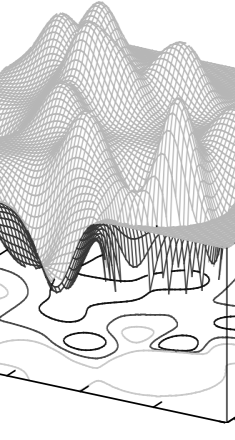
\includegraphics[height=7cm]{classPicture2-bw}
    }{\center

      \textbf{\fontsize{17}{20}\selectfont \course}

      ~

      %Lecture
      \topic\\

      \vspace{1cm}

      {\tiny~\emph{\keywords}~\\}

      \vspace{1cm}

      Marc Toussaint
      
      University of Stuttgart

      Summer 2019

      ~

    }
  }
}

\newcommand{\slide}[2]{
  \slidefont
  \incpage\begin{frame}
  \addcontentsline{toc}{section}{#1}
  \vfill
  {\headerfont #1} \vspace*{-2ex}
  \begin{itemize}\item[]~\\
    #2
  \end{itemize}
  \vfill
  \end{frame}
}

\newenvironment{slidecore}[1]{
  \slidefont\incpage
  \addcontentsline{toc}{section}{#1}
  \vfill
  {\headerfont #1} \vspace*{-2ex}
  \begin{itemize}\item[]~\\
}{
  \end{itemize}
  \vfill
}


\providecommand{\key}[1]{
  \addtocounter{mypage}{1}
% \immediate\write\keyfile{#1}
  \addtocontents{toc}{\hyperref[key:#1]{#1 (\arabic{mypage})}}
%  \phantomsection\label{key:#1}
%  \index{#1@{\hyperref[key:#1]{#1 (\arabic{mysec}:\arabic{mypage})}}|phantom}
  \addtocounter{mypage}{-1}
}

\providecommand{\course}{}

\providecommand{\subtopic}{}

\providecommand{\sublecture}[2]{
  \renewcommand{\subtopic}{#1}
  \slide{#1}{#2}
}

\providecommand{\story}[1]{
~

Motivation: {\tiny #1}\clearpage
}

\newenvironment{items}[1][9]{
\par\setlength{\unitlength}{1pt}\fontsize{#1}{#1}\linespread{1.2}\selectfont
\begin{list}{--}{\leftmargin4ex \rightmargin0ex \labelsep1ex \labelwidth2ex
\topsep0pt \parsep0ex \itemsep3pt}
}{
\end{list}
}

\providecommand{\slidesfoot}{
  \end{document}
}


  \slideshead
}

\providecommand{\exercises}{
  \newcommand{\exerciseshead}{
  \documentclass[10pt,fleqn]{article}
  \stdpackages

  \definecolor{bluecol}{rgb}{0,0,.5}
  \definecolor{greencol}{rgb}{0,.4,0}
  \definecolor{shadecolor}{gray}{0.9}
  \usepackage[
    %    pdftex%,
    %%    letterpaper,
    %    bookmarks,
    %    bookmarksnumbered,
    colorlinks,
    urlcolor=bluecol,
    citecolor=black,
    linkcolor=bluecol,
    %    pagecolor=bluecol,
    pdfborder={0 0 0},
    %pdfborderstyle={/S/U/W 1},
    %%    backref,     %link from bibliography back to sections
    %%    pagebackref, %link from bibliography back to pages
    %%    pdfstartview=FitH, %fitwidth instead of fit window
    pdfpagemode=UseNone, %UseOutlines, %bookmarks are displayed by acrobat
    pdftitle={\course},
    pdfauthor={Marc Toussaint},
    pdfkeywords={}
  ]{hyperref}
  \DeclareGraphicsExtensions{.pdf,.png,.jpg,.eps}

  \renewcommand{\r}{\varrho}
  \renewcommand{\l}{\lambda}
  \renewcommand{\L}{\Lambda}
  \renewcommand{\b}{\beta}
  \renewcommand{\d}{\delta}
  \renewcommand{\k}{\kappa}
  \renewcommand{\t}{\theta}
  \renewcommand{\O}{\Omega}
  \renewcommand{\o}{\omega}
  \renewcommand{\SS}{{\cal S}}
  \renewcommand{\=}{\!=\!}
  %\renewcommand{\boldsymbol}{}
  %\renewcommand{\Chapter}{\chapter}
  %\renewcommand{\Subsection}{\subsection}

  \renewcommand{\baselinestretch}{1.1}
  \geometry{a4paper,headsep=7mm,hdivide={15mm,*,15mm},vdivide={20mm,*,15mm}}

  \fancyhead[L]{\thetitle, \textit{Marc Toussaint}---\today}
  \fancyhead[R]{\thepage}
  \fancyhead[C]{}
  \fancyfoot{}
  \pagestyle{fancy}

  \parindent 0pt
  \parskip 0.5ex

  \newcommand{\codefont}{\helvetica{8}{1.2}{m}{n}}

  \input{../shared/macros}

  \DefineShortVerb{\@}

  \newcounter{solutions}
  \setcounter{solutions}{1}
  \newenvironment{solution}{
    \small
    \begin{shaded}
  }{
    \end{shaded}
  }
  
  \renewcommand{\hat}{\widehat}
  \newcommand{\bbg}{{\bar{\bar g}}}
  \graphicspath{{pics/}{../shared/pics/}}

  \renewcommand{\labelenumi}{{\alph{enumi})}}

  %%%%%%%%%%%%%%%%%%%%%%%%%%%%%%%%%%%%%%%%%%%%%%%%%%%%%%%%%%%%%%%%%%%%%%%%%%%%%%%%


  \mytitle{\course\\Exercise \exnum}
  \myauthor{Marc Toussaint\\ TAs: Janik Hager, Philipp Kratzer\\\small\addressUSTT}
  
  
  \begin{document}
  \onecolumn
  \maketitle
}

\newcommand{\exsection}[1]{\section{#1}}

\newcommand{\exerfoot}{
  \end{document}
}

\newenvironment{items}[1][9]{
  \par\setlength{\unitlength}{1pt}\fontsize{#1}{#1}\linespread{1.2}\selectfont
  \begin{list}{--}{\leftmargin4ex \rightmargin0ex \labelsep1ex \labelwidth2ex
      \topsep0pt \parsep0ex \itemsep3pt}
}{
  \end{list}
}

  \exerciseshead
}

\providecommand{\script}{
  \newcommand{\scripthead}{
  \documentclass[9pt,twoside]{article}
  \stdpackages

  \usepackage{palatino}
  \usepackage[envcountsect]{beamerarticle}
  \usepackage{makeidx}
  \makeindex

  \definecolor{bluecol}{rgb}{0,0,.5}
  \definecolor{greencol}{rgb}{0,.4,0}
  \definecolor{shadecolor}{gray}{0.9}
  \usepackage[
    %    pdftex%,
    %%    letterpaper,
    %bookmarks,
    bookmarksnumbered,
    colorlinks,
    urlcolor=bluecol,
    citecolor=black,
    linkcolor=bluecol,
    %    pagecolor=bluecol,
    pdfborder={0 0 0},
    %pdfborderstyle={/S/U/W 1},
    %%    backref,     %link from bibliography back to sections
    %%    pagebackref, %link from bibliography back to pages
    %%    pdfstartview=FitH, %fitwidth instead of fit window
    pdfpagemode=UseOutlines, %bookmarks are displayed by acrobat
    pdftitle={\course},
    pdfauthor={Marc Toussaint},
    pdfkeywords={}
  ]{hyperref}
  \DeclareGraphicsExtensions{.pdf,.png,.jpg,.eps}

  \usepackage{multimedia}
  %\setbeamercolor{background canvas}{bg=}

  \renewcommand{\r}{\varrho}
  \renewcommand{\l}{\lambda}
  \renewcommand{\L}{\Lambda}
  \renewcommand{\b}{\beta}
  \renewcommand{\d}{\delta}
  \renewcommand{\k}{\kappa}
  \renewcommand{\t}{\theta}
  \renewcommand{\O}{\Omega}
  \renewcommand{\o}{\omega}
  \renewcommand{\SS}{{\cal S}}
  \renewcommand{\=}{\!=\!}
  %\renewcommand{\boldsymbol}{}
  %\renewcommand{\Chapter}{\chapter}
  %\renewcommand{\Subsection}{\subsection}

  \renewcommand{\baselinestretch}{1.0}
  \geometry{a5paper,headsep=6mm,hdivide={10mm,*,10mm},vdivide={13mm,*,7mm}}

  \fancyhead[OL,ER]{\course, \textit{Marc Toussaint}}
  \fancyhead[OR,EL]{\thepage}
  \fancyhead[C]{}
  \fancyfoot{}
  \pagestyle{fancy}

%  \setcounter{tocdepth}{3}
  \setcounter{tocdepth}{2}

   \columnsep 6ex
  %  \renewcommand{\familydefault}{\sfdefault}
  \newcommand{\headerfont}{\large}%helvetica{12}{1}{b}{n}}
  \newcommand{\slidefont} {}%\helvetica{9}{1.3}{m}{n}}
  \newcommand{\storyfont} {}
  %  \renewcommand{\small}   {\helvetica{8}{1.2}{m}{n}}
  \renewcommand{\tiny}    {\footnotesize}%helvetica{7}{1.1}{m}{n}}
  \newcommand{\codefont}{\fontsize{6}{6}\selectfont}%helvetica{8}{1.2}{m}{n}}

  \input{../shared/macros}

  \DefineShortVerb{\@}

  \newcounter{solutions}
  \setcounter{solutions}{1}
  \renewenvironment{solution}{
    \small
    \begin{shaded}
  }{
    \end{shaded}
  }

  \graphicspath{{pics/}{../shared/pics/}}

%%%%%%%%%%%%%%%%%%%%%%%%%%%%%%%%%%%%%%%%%%%%%%%%%%%%%%%%%%%%%%%%%%%%%%%%%%%%%%%%

  \mytitle{\course\\Lecture Script}
  \myauthor{Marc Toussaint}

  \begin{document}

  %% \vspace*{2cm}

  \maketitle
  %\anchor{100,10}{\includegraphics[width=4cm]{optim}}

%  \vspace*{1cm}

  \emph{This is a direct concatenation and reformatting of all lecture
    slides and exercises from the \emph{Machine Learning} course (summer
    term 2019, U Stuttgart), including indexing to help
    prepare for exams.}

  \emph{Double-starred** sections and slides are not relevant for the exam.}

  {\tableofcontents}
}

%%%%%%%%%%%%%%%%%%%%%%%%%%%%%%%%%%%%%%%%%%%%%%%%%%%%%%%%%%%%%%%%%%%%%%%%%%%%%%%%

%% \renewcommand{\keywords}{}
%% \newcommand{\topic}{}
%% \renewcommand{\mypause}{}

  \newcounter{mypage}
  \setcounter{mypage}{0}
  \newcounter{mysec}
  \setcounter{mysec}{0}
  \newcommand{\incpage}{\addtocounter{mypage}{1}}
  \newcommand{\incsec} {\addtocounter{mysec}{1}}

\newcommand{\beginTocMinipage}{
  \addtocontents{toc}{\smallskip\noindent\hspace*{.036\columnwidth}}
  \addtocontents{toc}{\protect\begin{minipage}{.914\columnwidth}\small}
}
\newcommand{\closeTocMinipage}{
  \addtocontents{toc}{\protect\end{minipage}}
  \addtocontents{toc}{}
  \addtocontents{toc}{\medskip}
}

\renewcommand{\slides}[1][]{
  \clearpage
  \incsec
  \section{\topic}
  {\small #1}
  \beginTocMinipage
  \setcounter{mypage}{0}
  \smallskip\nopagebreak\hrule\medskip
}

\newcommand{\slidesfoot}{
  \closeTocMinipage
  \bigskip
}

\newcommand{\sublecture}[2]{
  \pagebreak[3]
  \incpage
  \closeTocMinipage
  \subsection{#1}
  {\storyfont #2}
  \beginTocMinipage
  {\hfill\tiny \textsf{\arabic{mysec}:\arabic{mypage}}}\nopagebreak%
  \smallskip\nopagebreak\hrule
}

\newcommand{\key}[1]{
  \pagebreak[2]
  \addtocounter{mypage}{1}
  \addtocontents{toc}{\hyperref[key:#1]{#1 (\arabic{mysec}:\arabic{mypage})}}
  \phantomsection\label{key:#1}
  \index{#1@{\hyperref[key:#1]{#1 (\arabic{mysec}:\arabic{mypage})}}|phantom}
  \addtocounter{mypage}{-1}
}

\newenvironment{slidecore}[1]{
  \incpage
  \subsubsection*{#1}%{\headerfont\noindent\textbf{#1}\\}%
  \vspace{-6ex}%
  \begin{list}{$\bullet$}{\leftmargin4ex \rightmargin0ex \labelsep1ex
    \labelwidth2ex \partopsep0ex \topsep0ex \parsep.5ex \parskip0ex \itemsep0pt}\item[]~\\\nopagebreak%
}{
  \end{list}\nopagebreak%
  {\hfill\tiny \textsf{\arabic{mysec}:\arabic{mypage}}}\nopagebreak%
  \smallskip\nopagebreak\hrule
}

\newcommand{\slide}[2]{
  \begin{slidecore}{#1}
    #2
  \end{slidecore}
}

\newcommand{\exsection}[1]{
  \subsubsection{#1}
}

\renewcommand{\exercises}{
  \subsection{Exercise \exnum}
}

\newcommand{\exerfoot}{
  \bigskip
}

\newcommand{\story}[1]{
  \subsection*{Motivation \& Outline}
  \addtocontents{toc}{\hyperref[mot\arabic{mysec}]{Motivation \& Outline}}
  \phantomsection\label{mot\arabic{mysec}}
  {\storyfont\sf #1}
  \medskip\nopagebreak\hrule
}

\newcounter{savedsection}
\newcommand{\subappendix}{\setcounter{savedsection}{\arabic{section}}\appendix}
\newcommand{\noappendix}{
  \setcounter{section}{\arabic{savedsection}}% restore section number
  \setcounter{subsection}{0}% reset section counter
%  \gdef\@chapapp{\sectionname}% reset section name
  \renewcommand{\thesection}{\arabic{section}}% make section numbers arabic
}

\newenvironment{items}[1][9]{
\par\setlength{\unitlength}{1pt}\fontsize{#1}{#1}\linespread{1.2}\selectfont
\begin{list}{--}{\leftmargin4ex \rightmargin0ex \labelsep1ex \labelwidth2ex
\topsep0pt \parsep0ex \itemsep3pt}
}{
\end{list}
}

  \scripthead
}

\providecommand{\course}{NO COURSE}
\providecommand{\topic}{NO TOPIC}
\providecommand{\keywords}{NO KEYWORDS}
\providecommand{\exnum}{NO NUMBER}


\providecommand{\stdpackages}{
  \usepackage{amsmath}
  \usepackage{amssymb}
  \usepackage{amsfonts}
  \allowdisplaybreaks
  \usepackage{amsthm}
  \usepackage{eucal}
  \usepackage{graphicx}
  \usepackage{color}
  \usepackage{geometry}
  \usepackage{framed}
%  \usecolor{xcolor}
  \definecolor{shadecolor}{gray}{0.9}
  \setlength{\FrameSep}{3pt}
  \usepackage{fancyvrb}
  \fvset{numbers=left,xleftmargin=5ex}

  \usepackage{multicol} 
  \usepackage{fancyhdr}
}

\providecommand{\addressUSTT}{
  Machine~Learning~\&~Robotics~lab, U~Stuttgart\\\small
  Universit{\"a}tsstra{\ss}e 38, 70569~Stuttgart, Germany
}


\renewcommand{\course}{Robotics}
\renewcommand{\coursepicture}{roboticsLecture}
\renewcommand{\coursedate}{Winter 2014}
\renewcommand{\topic}{Path Planning}

\slides

%%%%%%%%%%%%%%%%%%%%%%%%%%%%%%%%%%%%%%%%%%%%%%%%%%%%%%%%%%%%%%%%%%%%%%%%%%%%%%%%
\key{Path finding examples}
\slide{Path finding examples}{

~

\mov{\show[.3]{alphaPuzzle}\qquad}{10-RoboticsLecture/alphaPuzzle.mpg}

~

\hfill{Alpha-Puzzle, solved with James Kuffner's RRTs}

}

%%%%%%%%%%%%%%%%%%%%%%%%%%%%%%%%%%%%%%%%%%%%%%%%%%%%%%%%%%%%%%%%%%%%%%%%%%%%%%%%

\slide{Path finding examples}{

~

\show[.7]{footsteps}

~

J. Kuffner, K. Nishiwaki, S. Kagami, M. Inaba, and H. Inoue. Footstep
Planning Among Obstacles for Biped Robots. Proc. IEEE/RSJ
Int. Conf. on Intelligent Robots and Systems (IROS), 2001.

}

%%%%%%%%%%%%%%%%%%%%%%%%%%%%%%%%%%%%%%%%%%%%%%%%%%%%%%%%%%%%%%%%%%%%%%%%%%%%%%%%

\slide{Path finding examples}{

~

\show{climbing}

~

T. Bretl. Motion Planning of Multi-Limbed Robots Subject to
Equilibrium Constraints: The Free-Climbing Robot
Problem. International Journal of Robotics Research, 25(4):317-342,
Apr 2006.  

}

%%%%%%%%%%%%%%%%%%%%%%%%%%%%%%%%%%%%%%%%%%%%%%%%%%%%%%%%%%%%%%%%%%%%%%%%%%%%%%%%

\slide{Path finding examples}{

~

\show[.4]{kinodynamic-planning}

~

S. M. LaValle and J. J. Kuffner. Randomized
Kinodynamic Planning. International Journal of Robotics Research,
20(5):378--400, May 2001.

}

%%%%%%%%%%%%%%%%%%%%%%%%%%%%%%%%%%%%%%%%%%%%%%%%%%%%%%%%%%%%%%%%%%%%%%%%%%%%%%%%
\key{Feedback control vs path finding vs trajectory optimization}
\slide{Feedback control, path finding, trajectory optim.}{

\show[.7]{planning}

~

\item Feedback Control: \quad E.g.,~ $q_{t\po} = q_t + J^\sharp (y^* - \phi(q_t))$

\item Trajectory Optimization: \quad $\argmin_{q_{0:T}} f(q_{0:T})$

\item Path Finding:~ Find some $q_{0:T}$ with only valid
configurations

%% \item word ``planning'' is ambigous

%% -- ``motion planning'' in Robotics often refers to path finding

%% -- ``planning'' in MDPs often means computing optimal policies

}

%%%%%%%%%%%%%%%%%%%%%%%%%%%%%%%%%%%%%%%%%%%%%%%%%%%%%%%%%%%%%%%%%%%%%%%%%%%%%%%%

%% \slide{Control, path finding, trajectory optimization}{

%% \item Combining methods:%

%% 1) Path Finding
%% \anchor{90,-60}{\showh[.45]{planning}}

%% 2) Trajectory Optimization (``smoothing'')

%% 3) Feedback Control

%% ~

%% ~

%% ~%\mypause

%% \item Many problems can be solved with only feedback control (though not optimally)

%% \item Many more problems can be solved \emph{locally} optimal with
%%   only trajectory optimization

%% \item Tricky problems need path finding: \emph{global} search for valid paths

%% }

%%%%%%%%%%%%%%%%%%%%%%%%%%%%%%%%%%%%%%%%%%%%%%%%%%%%%%%%%%%%%%%%%%%%%%%%%%%%%%%%
\slide{Outline}{

\item \textbf{Really briefly:} Heuristics \& Discretization (slides from Howie CHoset's CMU lectures)
\begin{items}
\item Bugs algorithm

\item Potentials to guide feedback control

\item Dijkstra
\end{items}

~

\item \textbf{Sample-based Path Finding}
\begin{items}
\item Probabilistic Roadmaps

\item Rapidly Exploring Random Trees
\end{items}

~

\item \textbf{Non-holonomic systems}


}

%%%%%%%%%%%%%%%%%%%%%%%%%%%%%%%%%%%%%%%%%%%%%%%%%%%%%%%%%%%%%%%%%%%%%%%%%%%%%%%%
\sublecture{Background}

%%%%%%%%%%%%%%%%%%%%%%%%%%%%%%%%%%%%%%%%%%%%%%%%%%%%%%%%%%%%%%%%%%%%%%%%%%%%%%%%
\key{Bug algorithms}
\slide{}{
\hspace*{-5mm}\includegraphics[page=6,width=1.\columnwidth]{choset/02-bugs.pdf}
}
\slide{}{
\hspace*{-5mm}\includegraphics[page=7,width=1.\columnwidth]{choset/02-bugs.pdf}
}
\slide{}{
\hspace*{-5mm}\includegraphics[page=8,width=1.\columnwidth]{choset/02-bugs.pdf}
}
\slide{}{
\hspace*{-5mm}\includegraphics[page=9,width=1.\columnwidth]{choset/02-bugs.pdf}
}

%%%%%%%%%%%%%%%%%%%%%%%%%%%%%%%%%%%%%%%%%%%%%%%%%%%%%%%%%%%%%%%%%%%%%%%%%%%%%%%%

%\includepdf[pages=-,pagecommand={\incpage}]{choset/03-boundaries.pdf}

\slide{BUG algorithms -- conclusions}{

\item Other variants: TangentBug, VisBug, RoverBug, WedgeBug, \dots

\item only 2D! ~ (TangentBug has extension to 3D)

\item Guaranteed convergence

\item Still active research:

K. Taylor and S.M. LaValle: \emph{
I-Bug: An Intensity-Based Bug Algorithm}

~

~

\item[$\To$] Useful for minimalistic, robust 2D goal reaching

-- not useful for finding paths in joint space

}

%%%%%%%%%%%%%%%%%%%%%%%%%%%%%%%%%%%%%%%%%%%%%%%%%%%%%%%%%%%%%%%%%%%%%%%%%%%%%%%%
\key{Potential fields}
\slide{}{
\hspace*{-5mm}\includegraphics[page=1,width=1.\columnwidth]{choset/04-potentials.pdf}
}
\slide{}{
\hspace*{-5mm}\includegraphics[page=1,width=1.\columnwidth]{choset/05-potentials.pdf}
}

\slide{}{
\hspace*{-5mm}\includegraphics[page=2,width=1.\columnwidth]{choset/05-potentials.pdf}
}

\slide{}{
\hspace*{-5mm}\includegraphics[page=3,width=1.\columnwidth]{choset/05-potentials.pdf}
}

%%%%%%%%%%%%%%%%%%%%%%%%%%%%%%%%%%%%%%%%%%%%%%%%%%%%%%%%%%%%%%%%%%%%%%%%%%%%%%%%
\slide{Potential fields -- conclusions}{

\item Very simple, therefore popular

\item In our framework: Combining a goal (endeffector) task variable,
with a constraint (collision avoidance) task variable; then using
inv.\ kinematics is \emph{exactly} the same as ``Potential Fields''

~

\item[$\To$] Does not solve locality problem of feedback control.

}

%%%%%%%%%%%%%%%%%%%%%%%%%%%%%%%%%%%%%%%%%%%%%%%%%%%%%%%%%%%%%%%%%%%%%%%%%%%%%%%%
\key{Dijkstra}
%\includepdf[pages=-,pagecommand={\incpage}]{choset/06-waveFront.pdf}
%includepdf[pages=1-8,pagecommand={\incpage}]{choset/07-waveFront.pdf}
\slide{}{
\hspace*{-5mm}\includegraphics[page=3,width=1.\columnwidth]{choset/07-waveFront.pdf}
}\slide{}{
\hspace*{-5mm}\includegraphics[page=2,width=1.\columnwidth]{choset/07-waveFront.pdf}
}\slide{}{
\hspace*{-5mm}\includegraphics[page=3,width=1.\columnwidth]{choset/07-waveFront.pdf}
}\slide{}{
\hspace*{-5mm}\includegraphics[page=4,width=1.\columnwidth]{choset/07-waveFront.pdf}
}\slide{}{
\hspace*{-5mm}\includegraphics[page=5,width=1.\columnwidth]{choset/07-waveFront.pdf}
}\slide{}{
\hspace*{-5mm}\includegraphics[page=6,width=1.\columnwidth]{choset/07-waveFront.pdf}
}\slide{}{
\hspace*{-5mm}\includegraphics[page=7,width=1.\columnwidth]{choset/07-waveFront.pdf}
}\slide{}{
\hspace*{-5mm}\includegraphics[page=8,width=1.\columnwidth]{choset/07-waveFront.pdf}
}


%%%%%%%%%%%%%%%%%%%%%%%%%%%%%%%%%%%%%%%%%%%%%%%%%%%%%%%%%%%%%%%%%%%%%%%%%%%%%%%%
\slide{Dijkstra Algorithm}{

\item Is efficient in \textbf{discrete domains}
\begin{items}
\item Given start and goal node in an arbitrary graph

\item Incrementally label nodes with their distance-from-start
\end{items}
~

\item Produces optimal (shortest) paths

~

\item Applying this to continuous domains requires discretization
\begin{items}
\item Grid-like discretization in high-dimensions is daunting! \emph{(curse of dimensionality)}

\item What are other ways to ``discretize'' space more efficiently?
\end{items}

}

%%%%%%%%%%%%%%%%%%%%%%%%%%%%%%%%%%%%%%%%%%%%%%%%%%%%%%%%%%%%%%%%%%%%%%%%%%%%%%%%
\sublecture{Sample-based Path Finding}

%%%%%%%%%%%%%%%%%%%%%%%%%%%%%%%%%%%%%%%%%%%%%%%%%%%%%%%%%%%%%%%%%%%%%%%%%%%%%%%%
\key{Probabilistic Road Maps (PRMs)}
\slide{Probabilistic Road Maps}{

\show{prm-1}

\hfill [Kavraki, Svetska, Latombe,Overmars, 95]

~\mypause

$q \in \RRR^n$ describes configuration

$\qfree$ is the set of configurations without collision

~

}

%%%%%%%%%%%%%%%%%%%%%%%%%%%%%%%%%%%%%%%%%%%%%%%%%%%%%%%%%%%%%%%%%%%%%%%%%%%%%%%%
\slide{Probabilistic Road Maps}{

\show{prm-1}

\hfill [Kavraki, Svetska, Latombe,Overmars, 95]

Probabilistic Road Map

\item generates a graph $G=(V,E)$ of configurations
\begin{items}
\item such that configurations along each edges are $\in\qfree$
\end{items}

}

%%%%%%%%%%%%%%%%%%%%%%%%%%%%%%%%%%%%%%%%%%%%%%%%%%%%%%%%%%%%%%%%%%%%%%%%%%%%%%%%
\slide{Probabilistic Road Maps}{

\show{prm-2}

~

Given the graph, use (e.g.) Dijkstra to find path from
$q_{\text{start}}$ to $q_{\text{goal}}$.

}

%%%%%%%%%%%%%%%%%%%%%%%%%%%%%%%%%%%%%%%%%%%%%%%%%%%%%%%%%%%%%%%%%%%%%%%%%%%%%%%%
\slide{Probabilistic Road Maps -- generation}{

\begin{algo}
\Require number $n$ of samples, number $k$ number of nearest
neighbors
\Ensure PRM $G=(V,E)$
\State initialize $V=\emptyset$, $E=\emptyset$
\While{$|V|<n$} \Comment{find $n$ collision free points $q_i$}
\State $q \gets$ {\color{red}random sample from $Q$}
\State \textbf{if} $q \in \qfree$ \textbf{then} $V\gets V \cup \{q\}$
\EndWhile
\ForAll{$q\in V$} \Comment{check if near points can be connected}
\State $N_q \gets k$ nearest neighbors of $q$ in $V$
\ForAll{$q'\in N_q$}
\State \textbf{if} {\color{red}path$(q,q') \in \qfree$} \textbf{then}  $E\gets E \cup \{(q,q')\}$
\EndFor
\EndFor
\end{algo}

~

where path$(q,q')$ is a local planner ~ (easiest: straight line)

}

%%%%%%%%%%%%%%%%%%%%%%%%%%%%%%%%%%%%%%%%%%%%%%%%%%%%%%%%%%%%%%%%%%%%%%%%%%%%%%%%
\key{Planning/testing local connections}
\slide{Local Planner}{

\show{prm-testing}

~

tests collisions up to a specified resolution $\d$

}

%%%%%%%%%%%%%%%%%%%%%%%%%%%%%%%%%%%%%%%%%%%%%%%%%%%%%%%%%%%%%%%%%%%%%%%%%%%%%%%%
\slide{Problem: Narrow Passages}{

~

\show{prm-passage}

~

The smaller the gap (clearance $\r$) the more unlikely to sample such
points.

}

%%%%%%%%%%%%%%%%%%%%%%%%%%%%%%%%%%%%%%%%%%%%%%%%%%%%%%%%%%%%%%%%%%%%%%%%%%%%%%%%
\key{Probabilistic completeness of PRMs}
\slide{PRM theory}{

(for uniform sampling in $d$-dim space)

\item Let $a,b \in \qfree$ and $\g$ a path in $\qfree$ connecting $a$
and $b$.

~

Then the probability that $PRM$ found the path after $n$ samples is
\begin{align*}
P(\text{PRM-success}\| n)
 &\ge 1 - \frac{2|\g|}{\r}~ e^{-\s \r^d n}
\end{align*}

$\s = \frac{|B_1|}{2^d |\qfree|}$

$\r =$ clearance of $\g$ ~ (distance to obstacles)

(roughly: the exponential term are ``volume ratios'')

~

\item This result is called \emph{probabilistic complete} (one can
achieve any probability with high enough $n$)

\item For a given success probability, $n$ needs to be exponential
in $d$

}

%%%%%%%%%%%%%%%%%%%%%%%%%%%%%%%%%%%%%%%%%%%%%%%%%%%%%%%%%%%%%%%%%%%%%%%%%%%%%%%%
\key{Other PRM sampling strategies}
\slide{Other PRM sampling strategies}{

~

\cen{
\showh[.3]{prm-sampling1}
\showh[.3]{prm-sampling2}
\showh[.3]{prm-sampling3}
}
\hfill{\tiny illustration from O. Brock's lecture}

~

{\helvetica{8}{1.2}{m}{n}
Gaussian: $q_1\sim \UU$; $q_2 \sim \NN(q_1,\s)$; if $q_1\in\qfree$
and $q_2 \not \in \qfree$, add $q_1$ (or vice versa).

Bridge: $q_1\sim \UU$; $q_2 \sim \NN(q_1,\s)$; $q_3 = (q_1+q_2)/2$; if
$q_1,q_2 \not\in\qfree$ and $q_3 \in \qfree$, add $q_3$.
}

\mypause

\item Sampling strategy can be made more intelligence: ``utility-based sampling''

\item Connection sampling

(once earlier sampling has produced connected components)


}

%%%%%%%%%%%%%%%%%%%%%%%%%%%%%%%%%%%%%%%%%%%%%%%%%%%%%%%%%%%%%%%%%%%%%%%%%%%%%%%%
\slide{Probabilistic Roadmaps -- conclusions}{

\item Pros:
\begin{items}
\item Algorithmically very simple

\item Highly explorative

\item Allows probabilistic performance guarantees

\item Good to answer many queries in an \emph{unchanged}
   environment
\end{items}

~

\item Cons:
\begin{items}
\item Precomputation of exhaustive roadmap takes a long time

(but not necessary for ``Lazy PRMs'')
\end{items}


}


%%%%%%%%%%%%%%%%%%%%%%%%%%%%%%%%%%%%%%%%%%%%%%%%%%%%%%%%%%%%%%%%%%%%%%%%%%%%%%%%
\slide{Rapidly Exploring Random Trees}{

2 motivations:

~

\item Single Query path finding: Focus computational efforts on paths for specific $(q_{\text{start}},q_{\text{goal}})$

~

\item Use actually controllable DoFs to incrementally explore the
search space: \emph{control-based} path finding.

~

(Ensures that RRTs can be extended to handling differential constraints.)

}

%%%%%%%%%%%%%%%%%%%%%%%%%%%%%%%%%%%%%%%%%%%%%%%%%%%%%%%%%%%%%%%%%%%%%%%%%%%%%%%%
\slide{}{

\center

\only<1>{\show[.5]{rrt1}}
\only<2>{\show[.5]{rrt2}}
\only<3>{\show[.5]{rrt3}}
\only<4>{\show[.5]{rrt4}}
\only<5>{\show[.5]{rrt5}}
\only<6>{\show[.5]{rrt6}}

~

\only<1>{$n=1$}
\only<2>{$n=100$}
\only<3>{$n=300$}
\only<4>{$n=600$}
\only<5>{$n=1000$}
\only<6>{$n=2000$}

}

%%%%%%%%%%%%%%%%%%%%%%%%%%%%%%%%%%%%%%%%%%%%%%%%%%%%%%%%%%%%%%%%%%%%%%%%%%%%%%%%
\key{Rapidly Exploring Random Trees (RRTs)}
\slide{Rapidly Exploring Random Trees}{

~

Simplest RRT with straight line local planner and step size
$\a$

~

\begin{algo}
\Require $q_{\text{start}}$, number $n$ of nodes, stepsize $\a$
\Ensure tree $T=(V,E)$
\State initialize $V=\{q_{\text{start}}\}$, $E=\emptyset$ 
\For{$i=0:n$}
\State $q_\target\gets$ random sample from $Q$
\State $q_\near\gets$ nearest neighbor of $q_\target$ in $V$
\State $q_\new\gets q_\near + \frac{\a}{|q_\target-q_\near|}(q_\target-q_\near)$
\State \textbf{if} $q_\new \in \qfree$ \textbf{then} $V\gets V \cup \{q_\new\}$,  $E\gets E \cup \{(q_\near,q_\new)\}$
\EndFor
\end{algo}

}

%%%%%%%%%%%%%%%%%%%%%%%%%%%%%%%%%%%%%%%%%%%%%%%%%%%%%%%%%%%%%%%%%%%%%%%%%%%%%%%%
\key{Goal-oriented RRT}
\slide{Rapidly Exploring Random Trees}{

~

RRT growing directedly towards the goal

~

\begin{algo}
\Require $q_{\text{start}}$, {\color{red}$q_{\text{goal}}$}, number $n$ of nodes, stepsize $\a$, {\color{red}$\b$}
\Ensure tree $T=(V,E)$
\State initialize $V=\{q_{\text{start}}\}$, $E=\emptyset$ 
\For{$i=0:n$}
\State {\color{red}\textbf{if} rand$(0,1)<\b$ \textbf{then} $q_\target\gets
q_{\text{goal}}$}
\State \textbf{else} $q_\target\gets$ random sample from $Q$
\State $q_\near\gets$ nearest neighbor of $q_\target$ in $V$
\State $q_\new\gets q_\near + \frac{\a}{|q_\target-q_\near|}(q_\target-q_\near)$
\State \textbf{if} $q_\new \in \qfree$ \textbf{then} $V\gets V \cup \{q_\new\}$,  $E\gets E \cup \{(q_\near,q_\new)\}$
\EndFor
\end{algo}

}

%%%%%%%%%%%%%%%%%%%%%%%%%%%%%%%%%%%%%%%%%%%%%%%%%%%%%%%%%%%%%%%%%%%%%%%%%%%%%%%%
\slide{}{

\center

\only<1>{\show[.5]{rrt1}}
\only<2>{\show[.5]{rrt7}}
\only<3>{\show[.5]{rrt8}}
\only<4>{\show[.5]{rrt9}}
\only<5>{\show[.5]{rrt10}}
\only<6>{\show[.5]{rrt11}}

~

\only<1>{$n=1$}
\only<2>{$n=100$}
\only<3>{$n=200$}
\only<4>{$n=300$}
\only<5>{$n=400$}
\only<6>{$n=500$}

}

%%%%%%%%%%%%%%%%%%%%%%%%%%%%%%%%%%%%%%%%%%%%%%%%%%%%%%%%%%%%%%%%%%%%%%%%%%%%%%%%
\key{Bi-directional RRT}
\slide{Bi-directional search}{

\item grow two trees starting from $q_{\text{start}}$ and
$q_{\text{goal}}$

~

\show[.4]{rrt12}

~

let one tree grow towards the other

(e.g., ``choose $q_\new$ of $T_1$ as
$q_\target$ of $T_2$'')


}

%%%%%%%%%%%%%%%%%%%%%%%%%%%%%%%%%%%%%%%%%%%%%%%%%%%%%%%%%%%%%%%%%%%%%%%%%%%%%%%%
\slide{Summary: RRTs}{

\item Pros (shared with PRMs):
\begin{items}
\item Algorithmically very simple

\item Highly explorative

\item Allows probabilistic performance guarantees
\end{items}

~

\item Pros (beyond PRMs):
\begin{items}
\item Focus computation on single query $(q_{\text{start}},
   q_{\text{goal}})$ problem

\item Trees from multiple queries can be merged to a roadmap

\item Can be extended to differential constraints (nonholonomic systems)
\end{items}

~

\item To keep in mind (shared with PRMs):
\begin{items}
\item The metric (for nearest neighbor selection) is sometimes critical

\item The local planner may be non-trivial
\end{items}

}

%%%%%%%%%%%%%%%%%%%%%%%%%%%%%%%%%%%%%%%%%%%%%%%%%%%%%%%%%%%%%%%%%%%%%%%%%%%%%%%%
\slide{References}{

Steven M. LaValle: \emph{Planning
Algorithms}, \url{http://planning.cs.uiuc.edu/}.

~

Choset et. al.: \emph{Principles of Motion Planning}, MIT Press.

~

Latombe's ``motion planning'' lecture,
\url{http://robotics.stanford.edu/~latombe/cs326/2007/schedule.htm}

}

%%%%%%%%%%%%%%%%%%%%%%%%%%%%%%%%%%%%%%%%%%%%%%%%%%%%%%%%%%%%%%%%%%%%%%%%%%%%%%%%
\slide{RRT*}{

Sertac Karaman \& Emilio Frazzoli: Incremental sampling-based
algorithms for optimal motion planning, arXiv 1005.0416 (2010).

~

\only<1>{\show[1]{rrt-star}}
\only<2>{\show[.5]{rrt-star2}}

}

%%%%%%%%%%%%%%%%%%%%%%%%%%%%%%%%%%%%%%%%%%%%%%%%%%%%%%%%%%%%%%%%%%%%%%%%%%%%%%%%
\sublecture{Non-holonomic systems}

%%%%%%%%%%%%%%%%%%%%%%%%%%%%%%%%%%%%%%%%%%%%%%%%%%%%%%%%%%%%%%%%%%%%%%%%%%%%%%%%
\key{Definition of non-holonomic}
\slide{Non-holonomic systems}{

\item We define a \textbf{nonholonomic system} as one with \textbf{differential constraints}:

\eqbox{$\dim(u_t)<\dim(x_t)$}

\cen{\emph{$\To$ Not all degrees of freedom are directly controllable}}

~

\item Dynamic systems are an example!

~

\item General definition of a differential constraint:

For any given state $x$, let $U_x$ be the tangent space that is
generated by controls:

\cen{$U_x = \{ \dot x ~:~ \dot x = f(x,u),~ u \in U \}$}

(non-holonomic $\iff \dim(U_x) < \dim(x)$)

~

The elements of $U_x$ are elements of $T_x$ subject to
additional \emph{differential constraints}.

}

%%%%%%%%%%%%%%%%%%%%%%%%%%%%%%%%%%%%%%%%%%%%%%%%%%%%%%%%%%%%%%%%%%%%%%%%%%%%%%%%
\slide{Car example}{

\twocol{.5}{.4}{
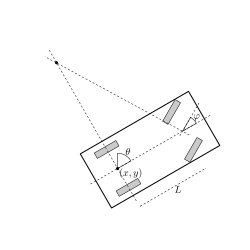
\includegraphics[width=.8\columnwidth]{car}
}{

$\dot x = v~ \cos \t$

$\dot y = v~ \sin \t$

$\dot \t = (v/L)~ \tan \varphi$

$|\varphi| < \Phi$
}

~

~

\cen{\textbf{State} $q = \mat{c}{x \\ y \\ \t}$
\qquad
\textbf{Controls} $u = \mat{c}{v \\ \varphi}$}

\cen{\textbf{Sytem equation} \qquad $\mat{c}{\dot x \\ \dot y \\ \dot \t}
= \mat{c}{v~ \cos \t \\ v~ \sin \t \\ (v/L)~ \tan \varphi }$}

}

%%%%%%%%%%%%%%%%%%%%%%%%%%%%%%%%%%%%%%%%%%%%%%%%%%%%%%%%%%%%%%%%%%%%%%%%%%%%%%%%
\slide{Car example}{

\item The car is a \emph{non-holonomic} system: not all DoFs are controlled, $\dim(u) < \dim(q)$

We have the \emph{differential constraint} $\dot q$:
\begin{align*}
\dot x \sin\t - \dot y \cos \t = 0
\end{align*}

``A car cannot move directly lateral.''

~

\small

\item Analogy to dynamic systems: Just like a car cannot instantly move
sidewards, a dynamic system cannot instantly change its position $q$:
the current change in position is \emph{constrained} by the current
velocity $\dot q$.

}

%%%%%%%%%%%%%%%%%%%%%%%%%%%%%%%%%%%%%%%%%%%%%%%%%%%%%%%%%%%%%%%%%%%%%%%%%%%%%%%%
\key{Path finding for a non-holonomic system}
\slide{Path finding for a non-holonomic system}{

Could a car follow this trajectory?

~

\cen{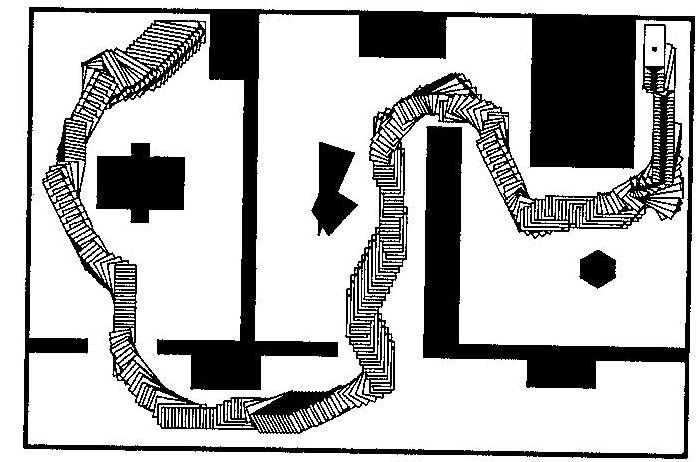
\includegraphics[width=.8\columnwidth]{car1-holonomic}}

This is generated with a PRM in the state space
$q=(x,y,\t)$ \emph{ignoring the differntial constraint}.

}

%%%%%%%%%%%%%%%%%%%%%%%%%%%%%%%%%%%%%%%%%%%%%%%%%%%%%%%%%%%%%%%%%%%%%%%%%%%%%%%%
\slide{Path finding with a non-holonomic system}{

This is a solution we would like to have:

~

\cen{\includegraphics[width=.8\columnwidth]{car3-smoothed}}

The path respects \textbf{differential constraints.}

Each step in the path corresponds to setting certain controls.

}


%%%%%%%%%%%%%%%%%%%%%%%%%%%%%%%%%%%%%%%%%%%%%%%%%%%%%%%%%%%%%%%%%%%%%%%%%%%%%%%%
\key{Control-based sampling}
\slide{Control-based sampling to grow a tree}{

~

\item Control-based sampling: fulfils none of the nice exploration
properties of RRTs, but fulfils the differential constraints:

~

1) Select a $q \in T$ from tree of current configurations

~

2) Pick control vector $u$ at random

~

3) Integrate equation of motion over short duration (picked at random or not)

~

4) If the motion is collision-free, add the endpoint to the tree

}

%%%%%%%%%%%%%%%%%%%%%%%%%%%%%%%%%%%%%%%%%%%%%%%%%%%%%%%%%%%%%%%%%%%%%%%%%%%%%%%%
\slide{Control-based sampling for the car}{

~

\twocol{.55}{.4}{
\includegraphics[width=.9\columnwidth]{car-tree-exploration}
}{

1) Select a $q \in T$

2) Pick $v$, $\p$, and $\tau$

3) Integrate motion from $q$

4) Add result if collision-free

}

}

%%%%%%%%%%%%%%%%%%%%%%%%%%%%%%%%%%%%%%%%%%%%%%%%%%%%%%%%%%%%%%%%%%%%%%%%%%%%%%%%
\slide{}{

\center

\includegraphics[width=.8\columnwidth]{car-parking1}

{\small J. Barraquand and J.C. Latombe. Nonholonomic Multibody Robots:
Controllability and Motion Planning in the Presence of
Obstacles. Algorithmica, 10:121-155, 1993.}

~

car parking

}

%%%%%%%%%%%%%%%%%%%%%%%%%%%%%%%%%%%%%%%%%%%%%%%%%%%%%%%%%%%%%%%%%%%%%%%%%%%%%%%%
\slide{}{

\center

\includegraphics[width=.6\columnwidth]{car-parking2}

~

car parking

}

%%%%%%%%%%%%%%%%%%%%%%%%%%%%%%%%%%%%%%%%%%%%%%%%%%%%%%%%%%%%%%%%%%%%%%%%%%%%%%%%
\slide{}{

\center

\includegraphics[width=.8\columnwidth]{car-parkingLeftOnly}

~

parking with only left-steering

}

%%%%%%%%%%%%%%%%%%%%%%%%%%%%%%%%%%%%%%%%%%%%%%%%%%%%%%%%%%%%%%%%%%%%%%%%%%%%%%%%

\slide{}{

\center

\includegraphics[width=.8\columnwidth]{car-withTrailer}

~

with a trailer

}

%%%%%%%%%%%%%%%%%%%%%%%%%%%%%%%%%%%%%%%%%%%%%%%%%%%%%%%%%%%%%%%%%%%%%%%%%%%%%%%%
\key{RRTs with differential constraints}
\slide{Better control-based exploration: RRTs revisited}{

\item RRTs with differential constraints:

\begin{algo}
\Require $q_{\text{start}}$, number $k$ of nodes, {\color{red}time interval $\tau$}
\Ensure tree $T=(V,E)$
\State initialize $V=\{q_{\text{start}}\}$, $E=\emptyset$ 
\For{$i=0:k$}
\State $q_\target\gets$ random sample from $Q$
\State $q_\near\gets$ {\color{red}nearest} neighbor of $q_\target$ in $V$
\State {\color{red}use local planner to compute controls $u$ that
steer $q_\near$ towards $q_\target$}
\State {\color{red} $q_\new \gets q_\near + \int\nolimits_{t=0}^\tau
\dot q(q,u) dt$}
\State \textbf{if} $q_\new \in \qfree$ \textbf{then} $V\gets V \cup \{q_\new\}$,  $E\gets E \cup \{(q_\near,q_\new)\}$
\EndFor
\end{algo}

~

\item Crucial questions:

\item How meassure \emph{near} in nonholonomic systems?

\item How find controls $u$ to steer towards target?

}

%%%%%%%%%%%%%%%%%%%%%%%%%%%%%%%%%%%%%%%%%%%%%%%%%%%%%%%%%%%%%%%%%%%%%%%%%%%%%%%%
\key{Configuration state metrics}
\slide{Configuration state metrics}{

{\small \hspace*{-5mm}Standard/Naive metrics:

\item Comparing two 2D rotations/orientations $\t_1, \t_2 \in SO(2)$:

~~ a) Euclidean metric between $e^{i\t_1}$ and $e^{i\t_2}$

~~ b) $d(\t_1, \t_2) = \min\{|\t_1-\t_2|, 2\pi - |\t_1-\t_2|\}$

\item Comparing two configurations $(x,y,\t)_{1,2}$ in $\RRR^2$:

~~ Eucledian metric on $(x,y,e^{i\t})$

\item Comparing two 3D rotations/orientations $r_1,r_2 \in SO(3)$:

~~ Represent both orientations as unit-length quaternions
$r_1,r_2 \in \RRR^4$:

\cen{$d(r_1,d_2) = \min\{|r_1-r_2| , |r_1+r_2|\}$}

~~ where $|\cdot|$ is the Euclidean metric.

~~ (Recall that $r_1$ and $-r_1$ represent exactly the same rotation.)

}

~\mypause

\item \textbf{Ideal metric:}

Optimal cost-to-go between two states $x_1$ and $x_2$:

\item Use optimal trajectory cost as metric

\item This is as hard to compute as the original problem, of course!!

$\to$ Approximate, e.g., by neglecting obstacles.

}

%%%%%%%%%%%%%%%%%%%%%%%%%%%%%%%%%%%%%%%%%%%%%%%%%%%%%%%%%%%%%%%%%%%%%%%%%%%%%%%%
\key{Side story: Dubins curves}
\slide{Side story: Dubins curves}{

\item Dubins car: constant velocity, and steer $\varphi \in
   [-\Phi,\Phi]$

~

\item Neglecting obstacles, there are only \textbf{six} types of
   trajectories that connect any configuration
   $\in \RRR^2\times\SSS^1$:

\cen{$\{ LRL, RLR, LSL, LSR, RSL, RSR \}$}

~

\item annotating durations of each phase:

\cen{$\{L_\a R_\b L_\g,
 , R_\a L_\b R_\g
 , L_\a S_d L_\g
 , L_\a S_d R_\g
 , R_\a S_d L_\g
 , R_\a S_d R_\g \}$}

with $\a\in[0,2\pi), \b\in(\pi,2\pi), d\ge0$

}

%%%%%%%%%%%%%%%%%%%%%%%%%%%%%%%%%%%%%%%%%%%%%%%%%%%%%%%%%%%%%%%%%%%%%%%%%%%%%%%%
\slide{Side story: Dubins curves}{\label{lastpage}

\includegraphics[width=.8\columnwidth]{dubins-curves}

~

$\to$ By testing all six types of trajectories for $(q_1,q_2)$ we can
define a Dubins metric for the RRT -- and use the Dubins curves as controls!

~\mypause

\item \textbf{Reeds-Shepp curves} are an extension for cars which can drive back.

(includes 46 types of trajectories, good metric for use in RRTs for
cars)

}

%%%%%%%%%%%%%%%%%%%%%%%%%%%%%%%%%%%%%%%%%%%%%%%%%%%%%%%%%%%%%%%%%%%%%%%%%%%%%%%%

%% \slide{Summary}{

%% \small
%% \hspace*{-5mm} We discuss 3 examples for dynamic/non-holonomic systems:

%% \item 1D point mass

%% -- We learnt about PID and the corresponding damped/oscilatory
%%    trajectories

%% \item General robot dynamics $M(q)~ \ddot q + C(q,\dot q)~ \dot q +
%%    G(q) = u$

%% -- We learnt how to follow a reference trajectory $q_{0:T}$ (joint
%%    space approach)

%% -- We learnt about optimal operational space control and following a
%%    task space trajectory $y_{0:T}$ (operational space control)

%% \item A car

%% -- We learnt about path finding under differential constraints

%% $\to$ This generalizes also to path finding for dynamic robots
%% (see LaValle's \emph{Planning Algorithms})

%% ~\mypause

%% \item We did not talk about trajectory \emph{optimization}. But the
%% general principle is obvious from slide \pageref{pageObjFunc}:

%% \cen{$f(u_{0:T}) = \sum_t \norm{u_t}_{H}^2 + \Phi_t(x_t)^\T \Phi_t(x_t)$}

%% where $x_t$ depends on the controls $u_{0:t\1}$, and $\Phi_t(x_t)$ can
%% be any task vector containing positional (as in the kinematic case) or
%% velocity-type task error.

%% }

%%%%%%%%%%%%%%%%%%%%%%%%%%%%%%%%%%%%%%%%%%%%%%%%%%%%%%%%%%%%%%%%%%%%%%%%%%%%%%%%

%% \slide{Collision detection issue}{

%% Sample-based path finding (both, PRMs and RRTs) heavily rely on
%% collision checking!

%% ~

%% $\to$ hierarchical collision checking

%% (Our simulator uses SWIFT++, other packages available,
%% e.g., \url{http://gamma.cs.unc.edu/research/collision/packages.html})

%% }

\slidesfoot


\providecommand{\slides}{
  \newcommand{\slideshead}{
  \newcommand{\thepage}{\arabic{mypage}}
  %beamer
  \documentclass[t,hyperref={bookmarks=true}]{beamer}
%  \documentclass[t,hyperref={bookmarks=true},aspectratio=169]{beamer}
  \setbeamersize{text margin left=5mm}
  \setbeamersize{text margin right=5mm}
  \usetheme{default}
  \usefonttheme[onlymath]{serif}
  \setbeamertemplate{navigation symbols}{}
  \setbeamertemplate{itemize items}{{\color{black}$\bullet$}}

  \newwrite\keyfile

  %\usepackage{palatino}
  \stdpackages
  \usepackage{multimedia}

  %%% geometry/spacing issues
  %
  \definecolor{bluecol}{rgb}{0,0,.5}
  \definecolor{greencol}{rgb}{0,.6,0}
  %\renewcommand{\baselinestretch}{1.1}
  \renewcommand{\arraystretch}{1.2}
  \columnsep 0mm

  \columnseprule 0pt
  \parindent 0ex
  \parskip 0ex
  %\setlength{\itemparsep}{3ex}
  %\renewcommand{\labelitemi}{\rule[3pt]{10pt}{10pt}~}
  %\renewcommand{\labelenumi}{\textbf{(\arabic{enumi})}}
  \newcommand{\headerfont}{\helvetica{13}{1.5}{b}{n}}
  \newcommand{\slidefont} {\helvetica{10}{1.4}{m}{n}}
  \newcommand{\codefont} {\helvetica{8}{1.2}{m}{n}}
  \renewcommand{\small} {\helvetica{9}{1.4}{m}{n}}
  \renewcommand{\tiny} {\helvetica{8}{1.3}{m}{n}}
  \newcommand{\ttiny} {\helvetica{7}{1.3}{m}{n}}

  %%% count pages properly and put the page number in bottom right
  %
  \newcounter{mypage}
  \newcommand{\incpage}{\addtocounter{mypage}{1}\setcounter{page}{\arabic{mypage}}}
  \setcounter{mypage}{0}
  \resetcounteronoverlays{page}

  \pagestyle{fancy}
  %\setlength{\headsep}{10mm}
  %\addtolength{\footheight}{15mm}
  \renewcommand{\headrulewidth}{0pt} %1pt}
  \renewcommand{\footrulewidth}{0pt} %.5pt}
  \cfoot{}
  \rhead{}
  \lhead{}
%  \rfoot{{\tiny\textsf{AI -- \topic -- \subtopic -- \arabic{mypage}/\pageref{lastpage}}}}
%  \rfoot{\vspace*{-4.5mm}{\tiny\textsf{\topic\ -- \subtopic\ -- \arabic{mypage}/\pageref{lastpage}}}\hspace*{-4mm}}
  \rfoot{\vspace*{-4.5mm}{\tiny\textsf{\color{gray}\topic\ -- \subtopic\ -- \arabic{mypage}/\pageref{lastpage}}}\hspace*{-4mm}}
  %\lfoot{\raisebox{5mm}{\tiny\textsf{\slideauthor}}}
  %\rfoot{\raisebox{5mm}{\tiny\textsf{\slidevenue{} -- \arabic{mypage}/\pageref{lastpage}}}}
  %\rfoot{~\anchor{30,12}{\tiny\textsf{\thepage/\pageref{lastpage}}}}
  %\lfoot{\small\textsf{Marc Toussaint}}

  \definecolor{grey}{rgb}{.8,.8,.8}
  \definecolor{head}{rgb}{.85,.9,.9}
  \definecolor{blue}{rgb}{.0,.0,.5}
  \definecolor{green}{rgb}{.0,.5,.0}
  \definecolor{red}{rgb}{.8,.0,.0}
  \newcommand{\inverted}{
    \definecolor{main}{rgb}{1,1,1}
    \color{main}
    \pagecolor[rgb]{.3,.3,.3}
  }
  \input{../shared/macros}

  \graphicspath{{pics/}{../shared/pics/}}

  \title{Machine Learning \topic}
  \author{Marc Toussaint}
  \institute{Machine Learning \& Robotics Lab, U Stuttgart}

  \begin{document}

  \rfoot{\vspace*{-5mm}{\tiny
  \textsf{\arabic{mypage}/\pageref{lastpage}}}\hspace*{-4mm}}

  %% title slide!
  \slide{}{
    \thispagestyle{empty}

    \twocol{.27}{.6}{
      \hspace*{-15mm}\includegraphics[height=7cm]{classPicture2-bw}
    }{\center

      \textbf{\fontsize{17}{20}\selectfont \course}

      ~

      %Lecture
      \topic\\

      \vspace{1cm}

      {\tiny~\emph{\keywords}~\\}

      \vspace{1cm}

      Marc Toussaint
      
      University of Stuttgart

      Summer 2019

      ~

    }
  }
}

\newcommand{\slide}[2]{
  \slidefont
  \incpage\begin{frame}
  \addcontentsline{toc}{section}{#1}
  \vfill
  {\headerfont #1} \vspace*{-2ex}
  \begin{itemize}\item[]~\\
    #2
  \end{itemize}
  \vfill
  \end{frame}
}

\newenvironment{slidecore}[1]{
  \slidefont\incpage
  \addcontentsline{toc}{section}{#1}
  \vfill
  {\headerfont #1} \vspace*{-2ex}
  \begin{itemize}\item[]~\\
}{
  \end{itemize}
  \vfill
}


\providecommand{\key}[1]{
  \addtocounter{mypage}{1}
% \immediate\write\keyfile{#1}
  \addtocontents{toc}{\hyperref[key:#1]{#1 (\arabic{mypage})}}
%  \phantomsection\label{key:#1}
%  \index{#1@{\hyperref[key:#1]{#1 (\arabic{mysec}:\arabic{mypage})}}|phantom}
  \addtocounter{mypage}{-1}
}

\providecommand{\course}{}

\providecommand{\subtopic}{}

\providecommand{\sublecture}[2]{
  \renewcommand{\subtopic}{#1}
  \slide{#1}{#2}
}

\providecommand{\story}[1]{
~

Motivation: {\tiny #1}\clearpage
}

\newenvironment{items}[1][9]{
\par\setlength{\unitlength}{1pt}\fontsize{#1}{#1}\linespread{1.2}\selectfont
\begin{list}{--}{\leftmargin4ex \rightmargin0ex \labelsep1ex \labelwidth2ex
\topsep0pt \parsep0ex \itemsep3pt}
}{
\end{list}
}

\providecommand{\slidesfoot}{
  \end{document}
}


  \slideshead
}

\providecommand{\exercises}{
  \newcommand{\exerciseshead}{
  \documentclass[10pt,fleqn]{article}
  \stdpackages

  \definecolor{bluecol}{rgb}{0,0,.5}
  \definecolor{greencol}{rgb}{0,.4,0}
  \definecolor{shadecolor}{gray}{0.9}
  \usepackage[
    %    pdftex%,
    %%    letterpaper,
    %    bookmarks,
    %    bookmarksnumbered,
    colorlinks,
    urlcolor=bluecol,
    citecolor=black,
    linkcolor=bluecol,
    %    pagecolor=bluecol,
    pdfborder={0 0 0},
    %pdfborderstyle={/S/U/W 1},
    %%    backref,     %link from bibliography back to sections
    %%    pagebackref, %link from bibliography back to pages
    %%    pdfstartview=FitH, %fitwidth instead of fit window
    pdfpagemode=UseNone, %UseOutlines, %bookmarks are displayed by acrobat
    pdftitle={\course},
    pdfauthor={Marc Toussaint},
    pdfkeywords={}
  ]{hyperref}
  \DeclareGraphicsExtensions{.pdf,.png,.jpg,.eps}

  \renewcommand{\r}{\varrho}
  \renewcommand{\l}{\lambda}
  \renewcommand{\L}{\Lambda}
  \renewcommand{\b}{\beta}
  \renewcommand{\d}{\delta}
  \renewcommand{\k}{\kappa}
  \renewcommand{\t}{\theta}
  \renewcommand{\O}{\Omega}
  \renewcommand{\o}{\omega}
  \renewcommand{\SS}{{\cal S}}
  \renewcommand{\=}{\!=\!}
  %\renewcommand{\boldsymbol}{}
  %\renewcommand{\Chapter}{\chapter}
  %\renewcommand{\Subsection}{\subsection}

  \renewcommand{\baselinestretch}{1.1}
  \geometry{a4paper,headsep=7mm,hdivide={15mm,*,15mm},vdivide={20mm,*,15mm}}

  \fancyhead[L]{\thetitle, \textit{Marc Toussaint}---\today}
  \fancyhead[R]{\thepage}
  \fancyhead[C]{}
  \fancyfoot{}
  \pagestyle{fancy}

  \parindent 0pt
  \parskip 0.5ex

  \newcommand{\codefont}{\helvetica{8}{1.2}{m}{n}}

  \input{../shared/macros}

  \DefineShortVerb{\@}

  \newcounter{solutions}
  \setcounter{solutions}{1}
  \newenvironment{solution}{
    \small
    \begin{shaded}
  }{
    \end{shaded}
  }
  
  \renewcommand{\hat}{\widehat}
  \newcommand{\bbg}{{\bar{\bar g}}}
  \graphicspath{{pics/}{../shared/pics/}}

  \renewcommand{\labelenumi}{{\alph{enumi})}}

  %%%%%%%%%%%%%%%%%%%%%%%%%%%%%%%%%%%%%%%%%%%%%%%%%%%%%%%%%%%%%%%%%%%%%%%%%%%%%%%%


  \mytitle{\course\\Exercise \exnum}
  \myauthor{Marc Toussaint\\ TAs: Janik Hager, Philipp Kratzer\\\small\addressUSTT}
  
  
  \begin{document}
  \onecolumn
  \maketitle
}

\newcommand{\exsection}[1]{\section{#1}}

\newcommand{\exerfoot}{
  \end{document}
}

\newenvironment{items}[1][9]{
  \par\setlength{\unitlength}{1pt}\fontsize{#1}{#1}\linespread{1.2}\selectfont
  \begin{list}{--}{\leftmargin4ex \rightmargin0ex \labelsep1ex \labelwidth2ex
      \topsep0pt \parsep0ex \itemsep3pt}
}{
  \end{list}
}

  \exerciseshead
}

\providecommand{\script}{
  \newcommand{\scripthead}{
  \documentclass[9pt,twoside]{article}
  \stdpackages

  \usepackage{palatino}
  \usepackage[envcountsect]{beamerarticle}
  \usepackage{makeidx}
  \makeindex

  \definecolor{bluecol}{rgb}{0,0,.5}
  \definecolor{greencol}{rgb}{0,.4,0}
  \definecolor{shadecolor}{gray}{0.9}
  \usepackage[
    %    pdftex%,
    %%    letterpaper,
    %bookmarks,
    bookmarksnumbered,
    colorlinks,
    urlcolor=bluecol,
    citecolor=black,
    linkcolor=bluecol,
    %    pagecolor=bluecol,
    pdfborder={0 0 0},
    %pdfborderstyle={/S/U/W 1},
    %%    backref,     %link from bibliography back to sections
    %%    pagebackref, %link from bibliography back to pages
    %%    pdfstartview=FitH, %fitwidth instead of fit window
    pdfpagemode=UseOutlines, %bookmarks are displayed by acrobat
    pdftitle={\course},
    pdfauthor={Marc Toussaint},
    pdfkeywords={}
  ]{hyperref}
  \DeclareGraphicsExtensions{.pdf,.png,.jpg,.eps}

  \usepackage{multimedia}
  %\setbeamercolor{background canvas}{bg=}

  \renewcommand{\r}{\varrho}
  \renewcommand{\l}{\lambda}
  \renewcommand{\L}{\Lambda}
  \renewcommand{\b}{\beta}
  \renewcommand{\d}{\delta}
  \renewcommand{\k}{\kappa}
  \renewcommand{\t}{\theta}
  \renewcommand{\O}{\Omega}
  \renewcommand{\o}{\omega}
  \renewcommand{\SS}{{\cal S}}
  \renewcommand{\=}{\!=\!}
  %\renewcommand{\boldsymbol}{}
  %\renewcommand{\Chapter}{\chapter}
  %\renewcommand{\Subsection}{\subsection}

  \renewcommand{\baselinestretch}{1.0}
  \geometry{a5paper,headsep=6mm,hdivide={10mm,*,10mm},vdivide={13mm,*,7mm}}

  \fancyhead[OL,ER]{\course, \textit{Marc Toussaint}}
  \fancyhead[OR,EL]{\thepage}
  \fancyhead[C]{}
  \fancyfoot{}
  \pagestyle{fancy}

%  \setcounter{tocdepth}{3}
  \setcounter{tocdepth}{2}

   \columnsep 6ex
  %  \renewcommand{\familydefault}{\sfdefault}
  \newcommand{\headerfont}{\large}%helvetica{12}{1}{b}{n}}
  \newcommand{\slidefont} {}%\helvetica{9}{1.3}{m}{n}}
  \newcommand{\storyfont} {}
  %  \renewcommand{\small}   {\helvetica{8}{1.2}{m}{n}}
  \renewcommand{\tiny}    {\footnotesize}%helvetica{7}{1.1}{m}{n}}
  \newcommand{\codefont}{\fontsize{6}{6}\selectfont}%helvetica{8}{1.2}{m}{n}}

  \input{../shared/macros}

  \DefineShortVerb{\@}

  \newcounter{solutions}
  \setcounter{solutions}{1}
  \renewenvironment{solution}{
    \small
    \begin{shaded}
  }{
    \end{shaded}
  }

  \graphicspath{{pics/}{../shared/pics/}}

%%%%%%%%%%%%%%%%%%%%%%%%%%%%%%%%%%%%%%%%%%%%%%%%%%%%%%%%%%%%%%%%%%%%%%%%%%%%%%%%

  \mytitle{\course\\Lecture Script}
  \myauthor{Marc Toussaint}

  \begin{document}

  %% \vspace*{2cm}

  \maketitle
  %\anchor{100,10}{\includegraphics[width=4cm]{optim}}

%  \vspace*{1cm}

  \emph{This is a direct concatenation and reformatting of all lecture
    slides and exercises from the \emph{Machine Learning} course (summer
    term 2019, U Stuttgart), including indexing to help
    prepare for exams.}

  \emph{Double-starred** sections and slides are not relevant for the exam.}

  {\tableofcontents}
}

%%%%%%%%%%%%%%%%%%%%%%%%%%%%%%%%%%%%%%%%%%%%%%%%%%%%%%%%%%%%%%%%%%%%%%%%%%%%%%%%

%% \renewcommand{\keywords}{}
%% \newcommand{\topic}{}
%% \renewcommand{\mypause}{}

  \newcounter{mypage}
  \setcounter{mypage}{0}
  \newcounter{mysec}
  \setcounter{mysec}{0}
  \newcommand{\incpage}{\addtocounter{mypage}{1}}
  \newcommand{\incsec} {\addtocounter{mysec}{1}}

\newcommand{\beginTocMinipage}{
  \addtocontents{toc}{\smallskip\noindent\hspace*{.036\columnwidth}}
  \addtocontents{toc}{\protect\begin{minipage}{.914\columnwidth}\small}
}
\newcommand{\closeTocMinipage}{
  \addtocontents{toc}{\protect\end{minipage}}
  \addtocontents{toc}{}
  \addtocontents{toc}{\medskip}
}

\renewcommand{\slides}[1][]{
  \clearpage
  \incsec
  \section{\topic}
  {\small #1}
  \beginTocMinipage
  \setcounter{mypage}{0}
  \smallskip\nopagebreak\hrule\medskip
}

\newcommand{\slidesfoot}{
  \closeTocMinipage
  \bigskip
}

\newcommand{\sublecture}[2]{
  \pagebreak[3]
  \incpage
  \closeTocMinipage
  \subsection{#1}
  {\storyfont #2}
  \beginTocMinipage
  {\hfill\tiny \textsf{\arabic{mysec}:\arabic{mypage}}}\nopagebreak%
  \smallskip\nopagebreak\hrule
}

\newcommand{\key}[1]{
  \pagebreak[2]
  \addtocounter{mypage}{1}
  \addtocontents{toc}{\hyperref[key:#1]{#1 (\arabic{mysec}:\arabic{mypage})}}
  \phantomsection\label{key:#1}
  \index{#1@{\hyperref[key:#1]{#1 (\arabic{mysec}:\arabic{mypage})}}|phantom}
  \addtocounter{mypage}{-1}
}

\newenvironment{slidecore}[1]{
  \incpage
  \subsubsection*{#1}%{\headerfont\noindent\textbf{#1}\\}%
  \vspace{-6ex}%
  \begin{list}{$\bullet$}{\leftmargin4ex \rightmargin0ex \labelsep1ex
    \labelwidth2ex \partopsep0ex \topsep0ex \parsep.5ex \parskip0ex \itemsep0pt}\item[]~\\\nopagebreak%
}{
  \end{list}\nopagebreak%
  {\hfill\tiny \textsf{\arabic{mysec}:\arabic{mypage}}}\nopagebreak%
  \smallskip\nopagebreak\hrule
}

\newcommand{\slide}[2]{
  \begin{slidecore}{#1}
    #2
  \end{slidecore}
}

\newcommand{\exsection}[1]{
  \subsubsection{#1}
}

\renewcommand{\exercises}{
  \subsection{Exercise \exnum}
}

\newcommand{\exerfoot}{
  \bigskip
}

\newcommand{\story}[1]{
  \subsection*{Motivation \& Outline}
  \addtocontents{toc}{\hyperref[mot\arabic{mysec}]{Motivation \& Outline}}
  \phantomsection\label{mot\arabic{mysec}}
  {\storyfont\sf #1}
  \medskip\nopagebreak\hrule
}

\newcounter{savedsection}
\newcommand{\subappendix}{\setcounter{savedsection}{\arabic{section}}\appendix}
\newcommand{\noappendix}{
  \setcounter{section}{\arabic{savedsection}}% restore section number
  \setcounter{subsection}{0}% reset section counter
%  \gdef\@chapapp{\sectionname}% reset section name
  \renewcommand{\thesection}{\arabic{section}}% make section numbers arabic
}

\newenvironment{items}[1][9]{
\par\setlength{\unitlength}{1pt}\fontsize{#1}{#1}\linespread{1.2}\selectfont
\begin{list}{--}{\leftmargin4ex \rightmargin0ex \labelsep1ex \labelwidth2ex
\topsep0pt \parsep0ex \itemsep3pt}
}{
\end{list}
}

  \scripthead
}

\providecommand{\course}{NO COURSE}
\providecommand{\topic}{NO TOPIC}
\providecommand{\keywords}{NO KEYWORDS}
\providecommand{\exnum}{NO NUMBER}


\providecommand{\stdpackages}{
  \usepackage{amsmath}
  \usepackage{amssymb}
  \usepackage{amsfonts}
  \allowdisplaybreaks
  \usepackage{amsthm}
  \usepackage{eucal}
  \usepackage{graphicx}
  \usepackage{color}
  \usepackage{geometry}
  \usepackage{framed}
%  \usecolor{xcolor}
  \definecolor{shadecolor}{gray}{0.9}
  \setlength{\FrameSep}{3pt}
  \usepackage{fancyvrb}
  \fvset{numbers=left,xleftmargin=5ex}

  \usepackage{multicol} 
  \usepackage{fancyhdr}
}

\providecommand{\addressUSTT}{
  Machine~Learning~\&~Robotics~lab, U~Stuttgart\\\small
  Universit{\"a}tsstra{\ss}e 38, 70569~Stuttgart, Germany
}


\renewcommand{\course}{Robotics}
\renewcommand{\coursepicture}{roboticsLecture}
\renewcommand{\coursedate}{Winter 2014}
\renewcommand{\topic}{Path Optimization -- briefly}

\slides

%%%%%%%%%%%%%%%%%%%%%%%%%%%%%%%%%%%%%%%%%%%%%%%%%%%%%%%%%%%%%%%%%%%%%%%%%%%%%%%%
\slide{Outline}{

\item These are only some very brief notes on path optimization

~

\item The aim is to explain how to \emph{formulate} the optimization
problem. Concerning the optimization algortihm itself, refer to the
\emph{Optimization} lecture.

}

%%%%%%%%%%%%%%%%%%%%%%%%%%%%%%%%%%%%%%%%%%%%%%%%%%%%%%%%%%%%%%%%%%%%%%%%%%%%%%%%
\key{From inverse kinematics to path costs}
\slide{From inverse kinematics to path costs}{

\item Recall our optimality principle of inverse kinematics
$$\argmin_q \norm{q-q_0}_W^2 + \norm{\Phi(q)}^2$$

\item A trajectory $q_{0:T}$ is a sequence of robot configurations
$q_t \in\RRR^n$

\item Consider the cost function
\begin{align*}
f(q_{0:T})
 = \sum_{t=0}^T \norm{q_{t\1}-q_t}_W^2
%\norm{\Psi_t(q_{t\myminus k},..,q_t)}^2
 + \sum_{t=0}^T \norm{\Phi_t(q_t)}^2
\end{align*}
\hfill{\tiny (where $(q_{\1}$ is a given prefix)}

\item $\norm{q_{t\1}-q_t}_W^2$ represents \textbf{control costs}

%$k$ denotes the \textbf{order} of the control costs

$\Phi_t(q_t)$ represents \textbf{task costs}

%(More generally, task costs could depend on $\Phi_t(q_{t\myminus k},..,q_t)$)

}

%%%%%%%%%%%%%%%%%%%%%%%%%%%%%%%%%%%%%%%%%%%%%%%%%%%%%%%%%%%%%%%%%%%%%%%%%%%%%%%%

\key{General $k$-order cost terms}
\slide{General $k$-order cost terms}{

{\tiny [Notation: $x_t$ instead of $q_t$ represents joint state]}

\begin{align*}
\min_{x_{0:T}}\quad&
\sum_{t=0}^{T} f_t(x_{t-k:t})^\T f_t(x_{t-k:t})
%~+~ \sum_{t,t'} k(t,t') x_t^\T x_{t'}
 \feed
\st&
 \forall_t:~ g_t(x_{t-k:t}) \le 0 \comma h_t(x_{t-k:t}) = 0 ~.
\end{align*}

}

%%%%%%%%%%%%%%%%%%%%%%%%%%%%%%%%%%%%%%%%%%%%%%%%%%%%%%%%%%%%%%%%%%%%%%%%%%%%%%%%
\slide{Cost terms}{

\item The $f_t(x_{t-k:t})$ terms can penalize various things:

~

\small
\begin{tabular}{|c|l|p{.3\columnwidth}|}
\hline
%$k=0$ & $f_t(x_t) = x_t - x_0$ & penalize offset from zero \\
$k=1$ & $f_t(x_{t\1},x_t) = x_t-x_{t\1}$ & penalize velocity \\
$k=2$ & $f_t(x_{t\2},..,x_t) = x_t-2x_{t\1}+x_{t\2}$ & penalize acceleration \\
$k=3$ & $f_t(x_{t\myminus 3},..,x_t) = x_t-3x_{t\1}+3x_{t\2}-x_{t\myminus 3}$ &
penalize jerk\\
\hline
\end{tabular}

or in some arbitrary task spaces

\begin{tabular}{|c|l|p{.2\columnwidth}|}
\hline
$k=0$ & $f_t(x_t) = \phi(x_t) - y^*$ & penalize offset in some task space \\
$k=1$ & $f_t(x_{t\1},x_t) = \phi x_t-\phi x_{t\1}$ & \\
$k=2$ & $f_t(x_{t\2},..,x_t) = \phi x_t-2\phi x_{t\1}+\phi x_{t\2}$ & \\
$k=3$ & $f_t(x_{t\myminus 3},..,x_t) = \phi x_t-3\phi x_{t\1}+3\phi
x_{t\2}-\phi x_{t\myminus 3}$ & \\
\hline
\end{tabular}

~

\item And terms $f_t$ can be stacked arbitrarily

}

%%%%%%%%%%%%%%%%%%%%%%%%%%%%%%%%%%%%%%%%%%%%%%%%%%%%%%%%%%%%%%%%%%%%%%%%%%%%%%%%
\key{Choice of optimizer}
\slide{Choice of optimizer}{\label{lastpage}

\begin{align*}
\min_{x_{0:T}}\quad&
\sum_{t=0}^{T} f_t(x_{t-k:t})^\T f_t(x_{t-k:t})
%~+~ \sum_{t,t'} k(t,t') x_t^\T x_{t'}
 \feed
\st&
 \forall_t:~ g_t(x_{t-k:t}) \le 0 \comma h_t(x_{t-k:t}) = 0 ~.
\end{align*}

~

\item Constrained optimization methods:
\begin{items}
\item Log-barrier, squared penalties
\item \textbf{Augmented Lagrangian}
\end{items}

~

\item Note: also the Lagrangian is the form of the
so-called \textbf{Gauss-Newton} form. The pseudo Hessian is a banded,
symmetric, positive-definite matrix.

}

\slidesfoot


\providecommand{\slides}{
  \newcommand{\slideshead}{
  \newcommand{\thepage}{\arabic{mypage}}
  %beamer
  \documentclass[t,hyperref={bookmarks=true}]{beamer}
%  \documentclass[t,hyperref={bookmarks=true},aspectratio=169]{beamer}
  \setbeamersize{text margin left=5mm}
  \setbeamersize{text margin right=5mm}
  \usetheme{default}
  \usefonttheme[onlymath]{serif}
  \setbeamertemplate{navigation symbols}{}
  \setbeamertemplate{itemize items}{{\color{black}$\bullet$}}

  \newwrite\keyfile

  %\usepackage{palatino}
  \stdpackages
  \usepackage{multimedia}

  %%% geometry/spacing issues
  %
  \definecolor{bluecol}{rgb}{0,0,.5}
  \definecolor{greencol}{rgb}{0,.6,0}
  %\renewcommand{\baselinestretch}{1.1}
  \renewcommand{\arraystretch}{1.2}
  \columnsep 0mm

  \columnseprule 0pt
  \parindent 0ex
  \parskip 0ex
  %\setlength{\itemparsep}{3ex}
  %\renewcommand{\labelitemi}{\rule[3pt]{10pt}{10pt}~}
  %\renewcommand{\labelenumi}{\textbf{(\arabic{enumi})}}
  \newcommand{\headerfont}{\helvetica{13}{1.5}{b}{n}}
  \newcommand{\slidefont} {\helvetica{10}{1.4}{m}{n}}
  \newcommand{\codefont} {\helvetica{8}{1.2}{m}{n}}
  \renewcommand{\small} {\helvetica{9}{1.4}{m}{n}}
  \renewcommand{\tiny} {\helvetica{8}{1.3}{m}{n}}
  \newcommand{\ttiny} {\helvetica{7}{1.3}{m}{n}}

  %%% count pages properly and put the page number in bottom right
  %
  \newcounter{mypage}
  \newcommand{\incpage}{\addtocounter{mypage}{1}\setcounter{page}{\arabic{mypage}}}
  \setcounter{mypage}{0}
  \resetcounteronoverlays{page}

  \pagestyle{fancy}
  %\setlength{\headsep}{10mm}
  %\addtolength{\footheight}{15mm}
  \renewcommand{\headrulewidth}{0pt} %1pt}
  \renewcommand{\footrulewidth}{0pt} %.5pt}
  \cfoot{}
  \rhead{}
  \lhead{}
%  \rfoot{{\tiny\textsf{AI -- \topic -- \subtopic -- \arabic{mypage}/\pageref{lastpage}}}}
%  \rfoot{\vspace*{-4.5mm}{\tiny\textsf{\topic\ -- \subtopic\ -- \arabic{mypage}/\pageref{lastpage}}}\hspace*{-4mm}}
  \rfoot{\vspace*{-4.5mm}{\tiny\textsf{\color{gray}\topic\ -- \subtopic\ -- \arabic{mypage}/\pageref{lastpage}}}\hspace*{-4mm}}
  %\lfoot{\raisebox{5mm}{\tiny\textsf{\slideauthor}}}
  %\rfoot{\raisebox{5mm}{\tiny\textsf{\slidevenue{} -- \arabic{mypage}/\pageref{lastpage}}}}
  %\rfoot{~\anchor{30,12}{\tiny\textsf{\thepage/\pageref{lastpage}}}}
  %\lfoot{\small\textsf{Marc Toussaint}}

  \definecolor{grey}{rgb}{.8,.8,.8}
  \definecolor{head}{rgb}{.85,.9,.9}
  \definecolor{blue}{rgb}{.0,.0,.5}
  \definecolor{green}{rgb}{.0,.5,.0}
  \definecolor{red}{rgb}{.8,.0,.0}
  \newcommand{\inverted}{
    \definecolor{main}{rgb}{1,1,1}
    \color{main}
    \pagecolor[rgb]{.3,.3,.3}
  }
  \input{../shared/macros}

  \graphicspath{{pics/}{../shared/pics/}}

  \title{Machine Learning \topic}
  \author{Marc Toussaint}
  \institute{Machine Learning \& Robotics Lab, U Stuttgart}

  \begin{document}

  \rfoot{\vspace*{-5mm}{\tiny
  \textsf{\arabic{mypage}/\pageref{lastpage}}}\hspace*{-4mm}}

  %% title slide!
  \slide{}{
    \thispagestyle{empty}

    \twocol{.27}{.6}{
      \hspace*{-15mm}\includegraphics[height=7cm]{classPicture2-bw}
    }{\center

      \textbf{\fontsize{17}{20}\selectfont \course}

      ~

      %Lecture
      \topic\\

      \vspace{1cm}

      {\tiny~\emph{\keywords}~\\}

      \vspace{1cm}

      Marc Toussaint
      
      University of Stuttgart

      Summer 2019

      ~

    }
  }
}

\newcommand{\slide}[2]{
  \slidefont
  \incpage\begin{frame}
  \addcontentsline{toc}{section}{#1}
  \vfill
  {\headerfont #1} \vspace*{-2ex}
  \begin{itemize}\item[]~\\
    #2
  \end{itemize}
  \vfill
  \end{frame}
}

\newenvironment{slidecore}[1]{
  \slidefont\incpage
  \addcontentsline{toc}{section}{#1}
  \vfill
  {\headerfont #1} \vspace*{-2ex}
  \begin{itemize}\item[]~\\
}{
  \end{itemize}
  \vfill
}


\providecommand{\key}[1]{
  \addtocounter{mypage}{1}
% \immediate\write\keyfile{#1}
  \addtocontents{toc}{\hyperref[key:#1]{#1 (\arabic{mypage})}}
%  \phantomsection\label{key:#1}
%  \index{#1@{\hyperref[key:#1]{#1 (\arabic{mysec}:\arabic{mypage})}}|phantom}
  \addtocounter{mypage}{-1}
}

\providecommand{\course}{}

\providecommand{\subtopic}{}

\providecommand{\sublecture}[2]{
  \renewcommand{\subtopic}{#1}
  \slide{#1}{#2}
}

\providecommand{\story}[1]{
~

Motivation: {\tiny #1}\clearpage
}

\newenvironment{items}[1][9]{
\par\setlength{\unitlength}{1pt}\fontsize{#1}{#1}\linespread{1.2}\selectfont
\begin{list}{--}{\leftmargin4ex \rightmargin0ex \labelsep1ex \labelwidth2ex
\topsep0pt \parsep0ex \itemsep3pt}
}{
\end{list}
}

\providecommand{\slidesfoot}{
  \end{document}
}


  \slideshead
}

\providecommand{\exercises}{
  \newcommand{\exerciseshead}{
  \documentclass[10pt,fleqn]{article}
  \stdpackages

  \definecolor{bluecol}{rgb}{0,0,.5}
  \definecolor{greencol}{rgb}{0,.4,0}
  \definecolor{shadecolor}{gray}{0.9}
  \usepackage[
    %    pdftex%,
    %%    letterpaper,
    %    bookmarks,
    %    bookmarksnumbered,
    colorlinks,
    urlcolor=bluecol,
    citecolor=black,
    linkcolor=bluecol,
    %    pagecolor=bluecol,
    pdfborder={0 0 0},
    %pdfborderstyle={/S/U/W 1},
    %%    backref,     %link from bibliography back to sections
    %%    pagebackref, %link from bibliography back to pages
    %%    pdfstartview=FitH, %fitwidth instead of fit window
    pdfpagemode=UseNone, %UseOutlines, %bookmarks are displayed by acrobat
    pdftitle={\course},
    pdfauthor={Marc Toussaint},
    pdfkeywords={}
  ]{hyperref}
  \DeclareGraphicsExtensions{.pdf,.png,.jpg,.eps}

  \renewcommand{\r}{\varrho}
  \renewcommand{\l}{\lambda}
  \renewcommand{\L}{\Lambda}
  \renewcommand{\b}{\beta}
  \renewcommand{\d}{\delta}
  \renewcommand{\k}{\kappa}
  \renewcommand{\t}{\theta}
  \renewcommand{\O}{\Omega}
  \renewcommand{\o}{\omega}
  \renewcommand{\SS}{{\cal S}}
  \renewcommand{\=}{\!=\!}
  %\renewcommand{\boldsymbol}{}
  %\renewcommand{\Chapter}{\chapter}
  %\renewcommand{\Subsection}{\subsection}

  \renewcommand{\baselinestretch}{1.1}
  \geometry{a4paper,headsep=7mm,hdivide={15mm,*,15mm},vdivide={20mm,*,15mm}}

  \fancyhead[L]{\thetitle, \textit{Marc Toussaint}---\today}
  \fancyhead[R]{\thepage}
  \fancyhead[C]{}
  \fancyfoot{}
  \pagestyle{fancy}

  \parindent 0pt
  \parskip 0.5ex

  \newcommand{\codefont}{\helvetica{8}{1.2}{m}{n}}

  \input{../shared/macros}

  \DefineShortVerb{\@}

  \newcounter{solutions}
  \setcounter{solutions}{1}
  \newenvironment{solution}{
    \small
    \begin{shaded}
  }{
    \end{shaded}
  }
  
  \renewcommand{\hat}{\widehat}
  \newcommand{\bbg}{{\bar{\bar g}}}
  \graphicspath{{pics/}{../shared/pics/}}

  \renewcommand{\labelenumi}{{\alph{enumi})}}

  %%%%%%%%%%%%%%%%%%%%%%%%%%%%%%%%%%%%%%%%%%%%%%%%%%%%%%%%%%%%%%%%%%%%%%%%%%%%%%%%


  \mytitle{\course\\Exercise \exnum}
  \myauthor{Marc Toussaint\\ TAs: Janik Hager, Philipp Kratzer\\\small\addressUSTT}
  
  
  \begin{document}
  \onecolumn
  \maketitle
}

\newcommand{\exsection}[1]{\section{#1}}

\newcommand{\exerfoot}{
  \end{document}
}

\newenvironment{items}[1][9]{
  \par\setlength{\unitlength}{1pt}\fontsize{#1}{#1}\linespread{1.2}\selectfont
  \begin{list}{--}{\leftmargin4ex \rightmargin0ex \labelsep1ex \labelwidth2ex
      \topsep0pt \parsep0ex \itemsep3pt}
}{
  \end{list}
}

  \exerciseshead
}

\providecommand{\script}{
  \newcommand{\scripthead}{
  \documentclass[9pt,twoside]{article}
  \stdpackages

  \usepackage{palatino}
  \usepackage[envcountsect]{beamerarticle}
  \usepackage{makeidx}
  \makeindex

  \definecolor{bluecol}{rgb}{0,0,.5}
  \definecolor{greencol}{rgb}{0,.4,0}
  \definecolor{shadecolor}{gray}{0.9}
  \usepackage[
    %    pdftex%,
    %%    letterpaper,
    %bookmarks,
    bookmarksnumbered,
    colorlinks,
    urlcolor=bluecol,
    citecolor=black,
    linkcolor=bluecol,
    %    pagecolor=bluecol,
    pdfborder={0 0 0},
    %pdfborderstyle={/S/U/W 1},
    %%    backref,     %link from bibliography back to sections
    %%    pagebackref, %link from bibliography back to pages
    %%    pdfstartview=FitH, %fitwidth instead of fit window
    pdfpagemode=UseOutlines, %bookmarks are displayed by acrobat
    pdftitle={\course},
    pdfauthor={Marc Toussaint},
    pdfkeywords={}
  ]{hyperref}
  \DeclareGraphicsExtensions{.pdf,.png,.jpg,.eps}

  \usepackage{multimedia}
  %\setbeamercolor{background canvas}{bg=}

  \renewcommand{\r}{\varrho}
  \renewcommand{\l}{\lambda}
  \renewcommand{\L}{\Lambda}
  \renewcommand{\b}{\beta}
  \renewcommand{\d}{\delta}
  \renewcommand{\k}{\kappa}
  \renewcommand{\t}{\theta}
  \renewcommand{\O}{\Omega}
  \renewcommand{\o}{\omega}
  \renewcommand{\SS}{{\cal S}}
  \renewcommand{\=}{\!=\!}
  %\renewcommand{\boldsymbol}{}
  %\renewcommand{\Chapter}{\chapter}
  %\renewcommand{\Subsection}{\subsection}

  \renewcommand{\baselinestretch}{1.0}
  \geometry{a5paper,headsep=6mm,hdivide={10mm,*,10mm},vdivide={13mm,*,7mm}}

  \fancyhead[OL,ER]{\course, \textit{Marc Toussaint}}
  \fancyhead[OR,EL]{\thepage}
  \fancyhead[C]{}
  \fancyfoot{}
  \pagestyle{fancy}

%  \setcounter{tocdepth}{3}
  \setcounter{tocdepth}{2}

   \columnsep 6ex
  %  \renewcommand{\familydefault}{\sfdefault}
  \newcommand{\headerfont}{\large}%helvetica{12}{1}{b}{n}}
  \newcommand{\slidefont} {}%\helvetica{9}{1.3}{m}{n}}
  \newcommand{\storyfont} {}
  %  \renewcommand{\small}   {\helvetica{8}{1.2}{m}{n}}
  \renewcommand{\tiny}    {\footnotesize}%helvetica{7}{1.1}{m}{n}}
  \newcommand{\codefont}{\fontsize{6}{6}\selectfont}%helvetica{8}{1.2}{m}{n}}

  \input{../shared/macros}

  \DefineShortVerb{\@}

  \newcounter{solutions}
  \setcounter{solutions}{1}
  \renewenvironment{solution}{
    \small
    \begin{shaded}
  }{
    \end{shaded}
  }

  \graphicspath{{pics/}{../shared/pics/}}

%%%%%%%%%%%%%%%%%%%%%%%%%%%%%%%%%%%%%%%%%%%%%%%%%%%%%%%%%%%%%%%%%%%%%%%%%%%%%%%%

  \mytitle{\course\\Lecture Script}
  \myauthor{Marc Toussaint}

  \begin{document}

  %% \vspace*{2cm}

  \maketitle
  %\anchor{100,10}{\includegraphics[width=4cm]{optim}}

%  \vspace*{1cm}

  \emph{This is a direct concatenation and reformatting of all lecture
    slides and exercises from the \emph{Machine Learning} course (summer
    term 2019, U Stuttgart), including indexing to help
    prepare for exams.}

  \emph{Double-starred** sections and slides are not relevant for the exam.}

  {\tableofcontents}
}

%%%%%%%%%%%%%%%%%%%%%%%%%%%%%%%%%%%%%%%%%%%%%%%%%%%%%%%%%%%%%%%%%%%%%%%%%%%%%%%%

%% \renewcommand{\keywords}{}
%% \newcommand{\topic}{}
%% \renewcommand{\mypause}{}

  \newcounter{mypage}
  \setcounter{mypage}{0}
  \newcounter{mysec}
  \setcounter{mysec}{0}
  \newcommand{\incpage}{\addtocounter{mypage}{1}}
  \newcommand{\incsec} {\addtocounter{mysec}{1}}

\newcommand{\beginTocMinipage}{
  \addtocontents{toc}{\smallskip\noindent\hspace*{.036\columnwidth}}
  \addtocontents{toc}{\protect\begin{minipage}{.914\columnwidth}\small}
}
\newcommand{\closeTocMinipage}{
  \addtocontents{toc}{\protect\end{minipage}}
  \addtocontents{toc}{}
  \addtocontents{toc}{\medskip}
}

\renewcommand{\slides}[1][]{
  \clearpage
  \incsec
  \section{\topic}
  {\small #1}
  \beginTocMinipage
  \setcounter{mypage}{0}
  \smallskip\nopagebreak\hrule\medskip
}

\newcommand{\slidesfoot}{
  \closeTocMinipage
  \bigskip
}

\newcommand{\sublecture}[2]{
  \pagebreak[3]
  \incpage
  \closeTocMinipage
  \subsection{#1}
  {\storyfont #2}
  \beginTocMinipage
  {\hfill\tiny \textsf{\arabic{mysec}:\arabic{mypage}}}\nopagebreak%
  \smallskip\nopagebreak\hrule
}

\newcommand{\key}[1]{
  \pagebreak[2]
  \addtocounter{mypage}{1}
  \addtocontents{toc}{\hyperref[key:#1]{#1 (\arabic{mysec}:\arabic{mypage})}}
  \phantomsection\label{key:#1}
  \index{#1@{\hyperref[key:#1]{#1 (\arabic{mysec}:\arabic{mypage})}}|phantom}
  \addtocounter{mypage}{-1}
}

\newenvironment{slidecore}[1]{
  \incpage
  \subsubsection*{#1}%{\headerfont\noindent\textbf{#1}\\}%
  \vspace{-6ex}%
  \begin{list}{$\bullet$}{\leftmargin4ex \rightmargin0ex \labelsep1ex
    \labelwidth2ex \partopsep0ex \topsep0ex \parsep.5ex \parskip0ex \itemsep0pt}\item[]~\\\nopagebreak%
}{
  \end{list}\nopagebreak%
  {\hfill\tiny \textsf{\arabic{mysec}:\arabic{mypage}}}\nopagebreak%
  \smallskip\nopagebreak\hrule
}

\newcommand{\slide}[2]{
  \begin{slidecore}{#1}
    #2
  \end{slidecore}
}

\newcommand{\exsection}[1]{
  \subsubsection{#1}
}

\renewcommand{\exercises}{
  \subsection{Exercise \exnum}
}

\newcommand{\exerfoot}{
  \bigskip
}

\newcommand{\story}[1]{
  \subsection*{Motivation \& Outline}
  \addtocontents{toc}{\hyperref[mot\arabic{mysec}]{Motivation \& Outline}}
  \phantomsection\label{mot\arabic{mysec}}
  {\storyfont\sf #1}
  \medskip\nopagebreak\hrule
}

\newcounter{savedsection}
\newcommand{\subappendix}{\setcounter{savedsection}{\arabic{section}}\appendix}
\newcommand{\noappendix}{
  \setcounter{section}{\arabic{savedsection}}% restore section number
  \setcounter{subsection}{0}% reset section counter
%  \gdef\@chapapp{\sectionname}% reset section name
  \renewcommand{\thesection}{\arabic{section}}% make section numbers arabic
}

\newenvironment{items}[1][9]{
\par\setlength{\unitlength}{1pt}\fontsize{#1}{#1}\linespread{1.2}\selectfont
\begin{list}{--}{\leftmargin4ex \rightmargin0ex \labelsep1ex \labelwidth2ex
\topsep0pt \parsep0ex \itemsep3pt}
}{
\end{list}
}

  \scripthead
}

\providecommand{\course}{NO COURSE}
\providecommand{\topic}{NO TOPIC}
\providecommand{\keywords}{NO KEYWORDS}
\providecommand{\exnum}{NO NUMBER}


\providecommand{\stdpackages}{
  \usepackage{amsmath}
  \usepackage{amssymb}
  \usepackage{amsfonts}
  \allowdisplaybreaks
  \usepackage{amsthm}
  \usepackage{eucal}
  \usepackage{graphicx}
  \usepackage{color}
  \usepackage{geometry}
  \usepackage{framed}
%  \usecolor{xcolor}
  \definecolor{shadecolor}{gray}{0.9}
  \setlength{\FrameSep}{3pt}
  \usepackage{fancyvrb}
  \fvset{numbers=left,xleftmargin=5ex}

  \usepackage{multicol} 
  \usepackage{fancyhdr}
}

\providecommand{\addressUSTT}{
  Machine~Learning~\&~Robotics~lab, U~Stuttgart\\\small
  Universit{\"a}tsstra{\ss}e 38, 70569~Stuttgart, Germany
}


\renewcommand{\course}{Robotics}
\renewcommand{\coursepicture}{roboticsLecture}
\renewcommand{\coursedate}{Winter 2014}
\renewcommand{\topic}{Probabilities}

\slides

%%%%%%%%%%%%%%%%%%%%%%%%%%%%%%%%%%%%%%%%%%%%%%%%%%%%%%%%%%%%%%%%%%%%%%%%%%%%%%%%

\key{Probabilities as (subjective) information calculus}
\slide{Probability Theory}{

\item Why do we need probabilities?

~\mypause

-- Obvious: to express inherent (\emph{objective}) stochasticity of the world

~\mypause

\item But beyond this: ~ (also in a ``deterministic world''):
\begin{items}
\item lack of knowledge!

\item hidden (latent) variables

\item expressing \emph{uncertainty}

\item expressing \emph{information} ~ (and lack of information)

\item \textbf{Subjective Probability}
\end{items}

~

\item Probability Theory:~ an information calculus
      
}

%%%%%%%%%%%%%%%%%%%%%%%%%%%%%%%%%%%%%%%%%%%%%%%%%%%%%%%%%%%%%%%%%%%%%%%%%%%%%%%%

\slide{Outline}{

\item Basic definitions
\begin{items}
\item Random variables
\item joint, conditional, marginal distribution
\item Bayes' theorem
\end{items}

\item Probability distributions:
\begin{items}
%\item Binomial \& Beta
%\item Multinomial \& Dirichlet
%\item Conjugate priors
\item Gauss %; Wichart
%\item Student-t; Dirak; etc
\item Dirak \& Particles
\end{items}

%\item Utilities, decision theory, entropy, KLD

%\item Monte Carlo*

\emph{These are generic slides on probabilities I use throughout my
lecture. Only parts are relevant for this course.}

}

%%%%%%%%%%%%%%%%%%%%%%%%%%%%%%%%%%%%%%%%%%%%%%%%%%%%%%%%%%%%%%%%%%%%%%%%%%%%%%%%

\key{Frequentist vs Bayesian}
\slide{Probability: Frequentist and Bayesian}{

\item Frequentist probabilities are defined in the limit of
an infinite number of trials

{\small \emph{Example:} ``The probability of a particular coin
landing heads up is 0.43''

}

~

\item Bayesian (subjective) probabilities quantify degrees of belief

{\small \emph{Example:} ``The probability of it raining tomorrow is 0.3''

-- Not possible to repeat ``tomorrow''

}

}

%%%%%%%%%%%%%%%%%%%%%%%%%%%%%%%%%%%%%%%%%%%%%%%%%%%%%%%%%%%%%%%%%%%%%%%%%%%%%%%%
\sublecture{Basic definitions}{
}

%%%%%%%%%%%%%%%%%%%%%%%%%%%%%%%%%%%%%%%%%%%%%%%%%%%%%%%%%%%%%%%%%%%%%%%%%%%%%%%%
\key{Definitions based on sets}
\slide{Probabilities \& Sets}{

\item \textbf{Sample Space/domain} $\O$, ~ e.g. $\O = \{ 1,2,3,4,5,6\}$

~

\item \textbf{Probability} ~ $P:~ A\subset\O \mapsto [0,1]$

e.g., $P(\{1\}) = \frac{1}{6}$,\quad
$P(\{4\}) = \frac{1}{6}$,\quad
$P(\{2,5\}) = \frac{1}{3}$,\quad

~

\item Axioms: $\forall A,B\subseteq\O$

-- Nonnegativity $P(A) \ge 0$

-- Additivity $P(A\cup B) = P(A)+P(B)$ ~ if $A\cap B= \emptyset$

-- Normalization $P(\O) = 1$

~

\item Implications

$0 \le P(A) \le 1$

$P(\emptyset) = 0$

$A\subseteq B \To P(A)\le P(B)$

$P(A\cup B) = P(A)+P(B) - P(A\cap B)$

$P(\O \setminus A) = 1 - P(A)$

}


%%%%%%%%%%%%%%%%%%%%%%%%%%%%%%%%%%%%%%%%%%%%%%%%%%%%%%%%%%%%%%%%%%%%%%%%%%%%%%%%

\key{Random variables}
\slide{Probabilities \& Random Variables}{


\item %A \defi{random variable} takes \defi{values} with a certain probability.

For a random variable $X$ with discrete domain $\dom(X) = \O$ we write:

$\forall_{x\in\O}:~ 0\le P(X\=x) \le 1$

$\sum_{x \in \O} P(X\=x) = 1$

~

{\small
Example: ~ A dice can take values $\O=\{1,..,6\}$.

$X$ is the random variable of a dice throw.

$P(X\=1) \in [0,1]$ is the probability that $X$ takes value $1$.

}

~%\mypause

\item {\small A bit more formally: a random variable is a map from a
measureable space to a domain (sample space) and thereby introduces a
probability measure on the domain (``assigns a probability to each
possible value'')

}


}

%%%%%%%%%%%%%%%%%%%%%%%%%%%%%%%%%%%%%%%%%%%%%%%%%%%%%%%%%%%%%%%%%%%%%%%%%%%%%%%%

\key{Probability distribution}
\slide{Probabilty Distributions}{

\item $P(X\=1) \in \RRR$ denotes a specific probability

$P(X)$ denotes the probability distribution ~ (function over $\O$)

~\mypause

{\small

Example: ~ A dice can take values $\O=\{1,2,3,4,5,6\}$.

By $P(X)$ we discribe the full distribution over possible values
$\{1,..,6\}$. These are 6 numbers that sum to one, usually stored in a
\emph{table}, e.g.: $[\frac{1}{6}, \frac{1}{6}, \frac{1}{6}, \frac{1}{6}, \frac{1}{6}, \frac{1}{6}]$

}

~

\item In implementations we typically represent distributions over
  discrete random variables as tables (arrays) of numbers

~

\item Notation for summing over a RV:

\small

In equation we often need to sum over RVs. We then write

\cen{$\sum_X P(X)~ \cdots$}

as shorthand for the explicit notation $\sum_{x\in\dom(X)} P(X\=x)~ \cdots$


}

%%%%%%%%%%%%%%%%%%%%%%%%%%%%%%%%%%%%%%%%%%%%%%%%%%%%%%%%%%%%%%%%%%%%%%%%%%%%%%%%

\key{Joint distribution}
\key{Marginal}
\key{Conditional distribution}
\slide{Joint distributions}{

Assume we have \emph{two} random variables $X$ and $Y$

\hspace*{30mm}\show[.25]{jointProbability}

\vspace*{-15mm}

\item Definitions:


\emph{Joint:} \quad $P(X,Y)$

\emph{Marginal:} \quad $P(X) = \sum_Y P(X,Y)$

\emph{Conditional:} \quad $P(X|Y) = \frac{P(X,Y)}{P(Y)}$

~

{\small The conditional is normalized: ~ $\forall_Y:~ \sum_X P(X|Y) = 1$}

~

\item 
$X$ is \emph{independent} of $Y$ iff: $P(X|Y) = P(X)$

{\small (table thinking: all columns of $P(X|Y)$ are equal)}

}

%%%%%%%%%%%%%%%%%%%%%%%%%%%%%%%%%%%%%%%%%%%%%%%%%%%%%%%%%%%%%%%%%%%%%%%%%%%%%%%%

\slide{Joint distributions}{

{\small
\emph{joint:} \quad $P(X,Y)$

\emph{marginal:} \quad $P(X) = \sum_Y P(X,Y)$

\emph{conditional:} \quad $P(X|Y) = \frac{P(X,Y)}{P(Y)}$
}

~

\item Implications of these definitions:

\emph{Product rule:} \quad $P(X,Y) = P(X|Y)~ P(Y) = P(Y|X)~ P(X)$ 

~

\emph{Bayes' Theorem:} \quad  $P(X|Y) = \frac{P(Y|X)~ P(X)}{P(Y)} $

~

}

%%%%%%%%%%%%%%%%%%%%%%%%%%%%%%%%%%%%%%%%%%%%%%%%%%%%%%%%%%%%%%%%%%%%%%%%%%%%%%%%

\key{Bayes' Theorem}
\slide{Bayes' Theorem}{

\Large\center

$$
P(X|Y) = \frac{P(Y|X)~ P(X)}{P(Y)}
$$

~

{$\text{posterior} ~=~
\frac{\text{likelihood} ~\cdot~ \text{prior}}{\text{normalization}}$\quad}

}

%%%%%%%%%%%%%%%%%%%%%%%%%%%%%%%%%%%%%%%%%%%%%%%%%%%%%%%%%%%%%%%%%%%%%%%%%%%%%%%%

\key{Multiple RVs, conditional independence}
\slide{Multiple RVs:}{

\item Analogously for $n$ random variables $X_{1:n}$ (stored as a rank
  $n$ tensor)

\emph{Joint}: \quad $P(X_{1:n})$

\emph{Marginal}: \quad $P(X_1) = \sum_{X_{2:n}} P(X_{1:n})$,

\emph{Conditional}: \quad $P(X_1|X_{2:n}) = \frac{P(X_{1:n})}{P(X_{2:n})}$

~

\item 
$X$ is \emph{conditionally independent} of $Y$ given $Z$ iff:

\cen{$P(X|Y,Z) = P(X|Z)$}

~

\item Product rule and Bayes' Theorem:

\small

\hspace*{-8mm}\twocol[.05]{.5}{.5}{\center

$P(X_{1:n}) = \prod_{i=1}^n P(X_i | X_{i\po:n})$

\medskip

$P(X_1|X_{2:n}) = \frac{P(X_2 | X_1, X_{3:n}) ~ P(X_1 |
  X_{3:n})}{P(X_2 | X_{3:n})}$

}{

$P(X,Z,Y) = P(X|Y,Z)~ P(Y|Z)~ P(Z)$

\medskip

$P(X|Y,Z) = \frac{P(Y|X,Z)~ P(X|Z)}{P(Y|Z)} $

\medskip

$P(X,Y|Z) = \frac{P(X,Z|Y)~ P(Y)}{P(Z)} $

}

}

%%%%%%%%%%%%%%%%%%%%%%%%%%%%%%%%%%%%%%%%%%%%%%%%%%%%%%%%%%%%%%%%%%%%%%%%%%%%%%%%
\sublecture{Probability distributions}{

~

\twocol{.4}{.5}{
\show{Bishop}
}{

Bishop, C. M.: \emph{Pattern Recognition and Machine Learning}.

Springer, 2006


\url{http://research.microsoft.com/en-us/um/people/cmbishop/prml/}

}

}

%%%%%%%%%%%%%%%%%%%%%%%%%%%%%%%%%%%%%%%%%%%%%%%%%%%%%%%%%%%%%%%%%%%%%%%%%%%%%%%%
\slide{}{

\item We skip Bernoulli \& Beta, Multinomial \& Dirichlet..

}

%%%%%%%%%%%%%%%%%%%%%%%%%%%%%%%%%%%%%%%%%%%%%%%%%%%%%%%%%%%%%%%%%%%%%%%%%%%%%%%%
\key{Bernoulli and Binomial distributions}
\slide{Bernoulli \& Binomial}{

\item We have a binary random variable $x \in \{0,1\}$ ~ (i.e.\ $\dom(x)=\{0,1\}$)

The \emph{Bernoulli} distribution is parameterized by a single
scalar $\m$,
\begin{align*}
P(x\=1\|\m)
&= \m \comma P(x\=0\|\m) = 1-\m \\
\Bern(x\|\m)
&= \m^x (1-\m)^{1-x}
%% \Exp{x}
%% &= m \comma \Var{x}=\m(1-\m)
\end{align*}

\item We have a data set of random variables $D=\{x_1,..,x_n\}$,
each $x_i\in\{0,1\}$. If each $x_i\sim \Bern(x_i\|\m)$ we have
\begin{align*}
\hspace*{-6mm}
P(D\|\m)
&= \Prod_{i=1}^n \Bern(x_i\|\m) = \Prod_{i=1}^n \m^{x_i} (1-\m)^{1-x_i} \\
\hspace*{-6mm}
\argmax_\m~ \log P(D\|\m)
&= \argmax_\m~ \sum_{i=1}^n x_i \log \m + (1-x_i) \log (1-\m)
 = \frac{1}{n} \sum_{i=1}^n x_i
\end{align*}

\item The \emph{Binomial distribution} is the distribution over the count
 $m=\sum_{i=1}^n x_i$
\begin{align*}
\Bin(m\|n,\m)
&= \mat{c}{n\\m}~ \m^m (1-\m)^{n-m} \comma \mat{c}{n\\m}=\frac{n!}{(n-m)!~ m!}
%% \Exp{m}
%% &= n\m \comma \Var{m}=n\m(1-\m)
\end{align*}

}

%%%%%%%%%%%%%%%%%%%%%%%%%%%%%%%%%%%%%%%%%%%%%%%%%%%%%%%%%%%%%%%%%%%%%%%%%%%%%%%%

\key{Beta}
\slide{Beta}{

\cen{\textbf{How to express uncertainty over a Bernoulli parameter $\m$}}

\item The \emph{Beta} distribution is over the interval $[0,1]$,
typically the parameter $\m$ of a Bernoulli:
\begin{align*}
\Beta(\m\|a,b)
&= \frac{1}{B(a,b)}~ \m^{a-1} (1-\m)^{b-1}
\end{align*}
with mean $\<\m\>=\frac{a}{a+b}$ and mode $\m^*=\frac{a-1}{a+b-2}$ for $a,b>1$

~

\item The crucial point is:
\begin{items}
\item Assume we are in a world with a ``Bernoulli source'' (e.g.,
binary bandit), but don't know its parameter $\m$
\item Assume we have a \emph{prior} distribution $P(\m)
= \Beta(\m\|a,b)$
\item Assume we collected some data $D=\{x_1,..,x_n\}$,
$x_i\in\{0,1\}$, with counts $a_D = \sum_i x_i$  of $[x_i\=1]$
and $b_D = \sum_i (1-x_i)$ of $[x_i\=0]$
\item The posterior is
\begin{align*}
P(\m\|D)
&= \frac{P(D\|\m)}{P(D)}~ P(\m)
 \propto \Bin(D\|\m)~ \Beta(\m\|a,b) \\
&\propto \m^{a_D} (1-\m)^{b_D}~ \m^{a-1} (1-\m)^{b-1}
 = \m^{a-1+a_D} (1-\m)^{b-1+b_D} \\
&= \Beta(\m\|a+a_D,b+b_D)
\end{align*}
\end{items}

}

%%%%%%%%%%%%%%%%%%%%%%%%%%%%%%%%%%%%%%%%%%%%%%%%%%%%%%%%%%%%%%%%%%%%%%%%%%%%%%%%

\slide{Beta}{

~

\cen{\emph{The prior is $\Beta(\m\|a,b)$, the posterior is
$\Beta(\m\|a+a_D,b+b_D)$}}

~

\item Conclusions:
\begin{items}
\item The semantics of $a$ and $b$ are counts of $[x_i\=1]$ and $[x_i\=0]$,
respectively
\item The Beta distribution is conjugate to the Bernoulli~ (explained
later)
\item With the Beta distribution we can represent beliefs (state of
knowledge) about uncertain $\m\in[0,1]$ and know how to update this
belief given data
\end{items}

}

%%%%%%%%%%%%%%%%%%%%%%%%%%%%%%%%%%%%%%%%%%%%%%%%%%%%%%%%%%%%%%%%%%%%%%%%%%%%%%%%

\slide{Beta}{

\show{betaDistribution}
{\hfill\tiny from Bishop}

}

%%%%%%%%%%%%%%%%%%%%%%%%%%%%%%%%%%%%%%%%%%%%%%%%%%%%%%%%%%%%%%%%%%%%%%%%%%%%%%%%

\key{Multinomial}
\slide{Multinomial}{

\item We have an integer random variable $x \in \{1,..,K\}$

The probability of a single $x$ can be parameterized by $\m=(\m_1,..,\m_K)$:
\begin{align*}
P(x\=k\|\m)
&= \m_k
\end{align*}
with the constraint $\sum_{k=1}^K \m_k=1$ (probabilities need to be normalized)

\item We have a data set of random variables $D=\{x_1,..,x_n\}$,
each $x_i\in\{1,..,K\}$. If each $x_i\sim P(x_i\|\m)$ we have
\begin{align*}
P(D\|\m)
&= \Prod_{i=1}^n \m_{x_i}
 = \Prod_{i=1}^n \Prod_{k=1}^K \m_k^{[x_i=k]}
 = \Prod_{k=1}^K \m_k^{m_k}
\end{align*}
where $m_k = \sum_{i=1}^n [x_i\=k]$ is the count of $[x_i\=k]$. The ML
estimator is
\begin{align*}
\argmax_\m~ \log P(D\|\m)
&= \frac{1}{n} (m_1,..,m_K) 
\end{align*}

\item The \emph{Multinomial distribution} is this distribution over
the counts $m_k$
\begin{align*}
\Mult(m_1,..,m_K\|n,\m)
&\propto \Prod_{k=1}^K \m_k^{m_k}
\end{align*}

}

%%%%%%%%%%%%%%%%%%%%%%%%%%%%%%%%%%%%%%%%%%%%%%%%%%%%%%%%%%%%%%%%%%%%%%%%%%%%%%%%

\key{Dirichlet}
\slide{Dirichlet}{

\cen{\textbf{How to express uncertainty over a Multinomial parameter $\m$}}

\item The \emph{Dirichlet} distribution is over the $K$-simplex, that
is, over $\m_1,..,\m_K\in[0,1]$ subject to the constraint
 $\sum_{k=1}^K \m_k=1$:
\begin{align*}
\Dir(\m\|\a)
&\propto~ \Prod_{k=1}^K \m_k^{\a_k-1}
\end{align*}
It is parameterized by $\a = (\a_1,..,\a_K)$, has mean
$\<\m_i\>=\frac{\a_i}{\sum_j\!\a_j}$ and mode $\m_i^*
= \frac{\a_i-1}{\sum_j\!\a_j-K}$ for $a_i>1$.

~

\item The crucial point is:
\begin{items}
\item Assume we are in a world with a ``Multinomial source'' (e.g.,
an integer bandit), but don't know its parameter $\m$
\item Assume we have a \emph{prior} distribution $P(\m)
= \Dir(\m\|\a)$
\item Assume we collected some data $D=\{x_1,..,x_n\}$,
$x_i\in\{1,..,K\}$, with counts $m_k = \sum_i [x_i\=k]$
\item The posterior is
\begin{align*}
P(\m\|D)
&= \frac{P(D\|\m)}{P(D)}~ P(\m)
 \propto \Mult(D\|\m)~ \Dir(\m\|a,b) \\
&\propto \Prod_{k=1}^K \m_k^{m_k}~ \Prod_{k=1}^K \m_k^{\a_k-1}
 = \Prod_{k=1}^K \m_k^{\a_k-1+m_k} \\
&= \Dir(\m\|\a+m)
\end{align*}
\end{items}

}

%%%%%%%%%%%%%%%%%%%%%%%%%%%%%%%%%%%%%%%%%%%%%%%%%%%%%%%%%%%%%%%%%%%%%%%%%%%%%%%%

\slide{Dirichlet}{

~

\cen{\emph{The prior is $\Dir(\m\|\a)$, the posterior is
$\Dir(\m\|\a+m)$}}

~

\item Conclusions:
\begin{items}
\item The semantics of $\a$ is the counts of $[x_i\=k]$
\item The Dirichlet distribution is conjugate to the Multinomial
\item With the Dirichlet distribution we can represent beliefs (state of
knowledge) about uncertain $\m$ of an integer random variable and know
how to update this belief given data
\end{items}

}

%%%%%%%%%%%%%%%%%%%%%%%%%%%%%%%%%%%%%%%%%%%%%%%%%%%%%%%%%%%%%%%%%%%%%%%%%%%%%%%%

\slide{Dirichlet}{

Illustrations for $\a=(0.1,0.1,0.1)$, $\a=(1,1,1)$ and $\a=(10,10,10)$:

\show{dirichletDistribution}

\hfill{\tiny from Bishop}

}

%%%%%%%%%%%%%%%%%%%%%%%%%%%%%%%%%%%%%%%%%%%%%%%%%%%%%%%%%%%%%%%%%%%%%%%%%%%%%%%%

\slide{Motivation for Beta \& Dirichlet distributions}{

\item Bandits:
\begin{items}
\item If we have binary [integer] bandits, the Beta [Dirichlet]
distribution is a way to represent and update beliefs
\item The belief space becomes discrete: The parameter $\a$ of the
prior is continuous, but the posterior updates live on a discrete
``grid'' (adding counts to $\a$)
\item We can in principle do belief planning using this
\end{items}

\item Reinforcement Learning:
\begin{items}
\item Assume we know that the world is a finite-state MDP, but do not know its
transition probability $P(s'\|s,a)$. For each $(s,a)$, $P(s'\|s,a)$ is a
distribution over the integer $s'$
\item Having a separate Dirichlet distribution for each $(s,a)$ is a
way to represent our belief about the world, that is, our belief about
$P(s'\|s,a)$
\item We can in principle do belief planning using this
$\to$ \emph{Bayesian Reinforcement Learning}
\end{items}

\item Dirichlet distributions are also used to model texts (word
distributions in text), images, or mixture distributions in general

}

%%%%%%%%%%%%%%%%%%%%%%%%%%%%%%%%%%%%%%%%%%%%%%%%%%%%%%%%%%%%%%%%%%%%%%%%%%%%%%%%

\key{Conjugate priors}
\slide{Conjugate priors}{

~

\item Assume you have data $D=\{x_1,..,x_n\}$ with likelihood
$$P(D \| \t)$$
that depends on an uncertain parameter $\t$

Assume you have a prior $P(\t)$

~

\item The prior $P(\t)$ is \textbf{conjugate} to the likelihood
$P(D\|\t)$ iff the posterior
$$P(\t\|D) \propto P(D\|\t)~ P(\t)$$
is in the \emph{same distribution class} as the prior $P(\t)$

~

\item Having a conjugate prior is very convenient, because then you
know how to update the belief given data

}

%%%%%%%%%%%%%%%%%%%%%%%%%%%%%%%%%%%%%%%%%%%%%%%%%%%%%%%%%%%%%%%%%%%%%%%%%%%%%%%%

\slide{Conjugate priors}{

~

\begin{tabular}{p{.32\columnwidth}|@{\quad}p{.4\columnwidth}}
likelihood & conjugate \\
\hline
Binomial $\Bin(D \| \m)$ & Beta $\Beta(\m \| a,b)$ \\
Multinomial $\Mult(D \| \m)$ & Dirichlet $\Dir(\m \| \a)$ \\
Gauss $\NN(x \| \m,\S)$ & Gauss $\NN(\m \| \m_0, A)$ \\
1D Gauss $\NN(x \| \m,\l^\1)$ & Gamma ${\rm Gam}(\l \| a,b)$ \\
$n$D Gauss $\NN(x \| \m,\L^\1)$ & Wishart ${\rm Wish}(\L \| W, \n)$ \\
$n$D Gauss $\NN(x \| \m,\L^\1)$ & Gauss-Wishart $\NN(\m\|\m_0,
(\b\L)^\1)~ {\rm Wish}(\L \| W, \n)$
\end{tabular}

}

%%%%%%%%%%%%%%%%%%%%%%%%%%%%%%%%%%%%%%%%%%%%%%%%%%%%%%%%%%%%%%%%%%%%%%%%%%%%%%%%

\slide{Distributions over continuous domain}{
}

%%%%%%%%%%%%%%%%%%%%%%%%%%%%%%%%%%%%%%%%%%%%%%%%%%%%%%%%%%%%%%%%%%%%%%%%%%%%%%%%

\key{Dirac distribution}
\slide{Distributions over continuous domain}{

\item Let $x$ be a continuous RV. The \defi{probability density
  function (pdf)} $p(x)\in[0,\infty)$ defines the probability 
$$P(a\le x \le b) = \int_a^b p(x)~ dx ~ \in[0,1]$$

The \defi{(cumulative) probability distribution} $F(y) = P(x \le y) = \int_{-\infty}^y dx~
p(x)\in[0,1]$ is the cumulative integral with $\lim_{y\to\infty} F(y) = 1$

~

{\small (In discrete domain: \emph{probability distribution} and
    \emph{probability mass function} $P(x)\in[0,1]$ are used
    synonymously.)

}

~

\item Two basic examples:

\textbf{Gaussian}: ~
$\NN(x \| \m,\S) = \frac{1}{\|2\pi \S\|^{1/2}}~ e^{-\half (x-\m)^\T~ \S^\1~ (x-\m)}$

\textbf{Dirac or $\d$} (``point particle'') ~
$\d(x) = 0$ except at $x=0$, $\int\d(x)~dx = 1$

$\d(x) = \frac{\del}{\del x} H(x)$ where $H(x) = [x\ge0] =$ Heavyside step function

}

%%%%%%%%%%%%%%%%%%%%%%%%%%%%%%%%%%%%%%%%%%%%%%%%%%%%%%%%%%%%%%%%%%%%%%%%%%%%%%%%

\key{Gaussian}
\slide{Gaussian distribution}{

~

\item 1-dim:~
$
\NN(x \| \m,\s^2) = \frac{1}{\|2\pi \s^2\|^{1/2}}~ e^{-\half
(x-\m)^2/\s^2 }
$\anchor{25,-10}{\showh[.25]{Figure1_13}}

\item $n$-dim Gaussian in \emph{normal form}:
%\anchor{10,-6}{\showh[.2]{Figure2_8b}}
\begin{align*}
\NN(x \| \m, \S)
 &= \frac{1}{\|2\pi \S\|^{1/2}}~ \exp\{-\half (x-\m)^\T~ \S^\1~ (x-\m)\}
\end{align*}
with \textbf{mean} $\m$ and \textbf{covariance} matrix $\S$. In \emph{canonical form}:
\begin{align}
\NN[x \| a, A]
 = \frac{\exp\{-\half a^\T A^\1a\}}{\|2\pi A^\1\|^{1/2}}~
   \exp\{-\half x^\T~ A~ x + x^\T a\}
\end{align}
with \textbf{precision} matrix $A = \S^\1$ and coefficient $a=\S^\1 \m$
(and mean $\m = A^\1 a$).

~

\item Gaussian identities: see {\tiny\url{http://ipvs.informatik.uni-stuttgart.de/mlr/marc/notes/gaussians.pdf}}

}

%%%%%%%%%%%%%%%%%%%%%%%%%%%%%%%%%%%%%%%%%%%%%%%%%%%%%%%%%%%%%%%%%%%%%%%%%%%%%%%%

\slide{Gaussian identities}{

\providecommand{\+}{\myplus}
\renewcommand{\-}{\,\text{-}\,}
\small

Symmetry: \qquad $\NN(x\|a,A) = \NN(a\|x,A) = \NN(x-a\|0,A)$

~

Product:\\
$\NN(x \| a,A)~ \NN(x \| b,B) 
 = \NN[x \| A^\1 a+B^\1 b, A^\1 + B^\1]~ \NN(a\|b,A+B)$
$\NN[x \| a,A]~ \NN[x \| b,B]
 = \NN[x \| a+b,A+B]~ \NN(A^\1 a \| B^\1 b, A^\1+B^\1)$

~

``Propagation'':\\
$\int_y \NN(x \| a + Fy, A)~ \NN(y \| b, B)~ dy
 = \NN(x \| a + Fb, A+FBF^\T)$

~

Transformation:\\
$ \NN(F x + f \| a,A)
 = \frac{1}{\|F\|}~ \NN(x \| ~ F^\1 (a-f),~ F^\1 AF^\mT) $

~

Marginal \& conditional:\\
$\NN\bigg( \arr{c}{x\\ y} \bigg| \arr{c}{a\\ b} ,~ 
         \arr{cc}{A & C\\ C^\T & B} \bigg)
 = \NN(x \| a,A) \cdot \NN(y \| b+C^\T A^\1(x\-a),~ B - C^\T A^\1 C)$

~

More Gaussian identities: see {\tiny\url{http://ipvs.informatik.uni-stuttgart.de/mlr/marc/notes/gaussians.pdf}}

}

%%%%%%%%%%%%%%%%%%%%%%%%%%%%%%%%%%%%%%%%%%%%%%%%%%%%%%%%%%%%%%%%%%%%%%%%%%%%%%%%

%% \slide{Gaussian prior and posterior}{

%% \item Assume we have data $D = \{x_1,..,x_n\}$, each $x_i\in\RRR^n$,
%% with likelihood
%% \begin{align*}
%% P(D\|\m,\S)
%% &= \Prod_i \NN(x_i\|\m,\S) \\
%% \argmax_\m~ P(D\|\m,\S)
%% &= \frac{1}{n}\sum_{i=1}^n x_i \\
%% \argmax_\S~ P(D\|\m,\S)
%% &= \frac{1}{n} \sum_{i=1}^n (x_i-\m)(x_i-\m)^\T
%% \end{align*}

%% \item Assume we are initially uncertain about $\m$ (but know $\S$). We
%% can express this uncertainty using again a Gaussian $\NN[\m \|
%% a,A]$. Given data we have
%% \begin{align*}
%% P(\m\|D)
%% &\propto P(D\|\m,\S)~ P(\m)
%%  = \Prod_i \NN(x_i\| \m,\S)~ \NN[\m \| a, A] \\
%% &= \Prod_i \NN[\m\| \S^\1 x_i,\S^\1]~ \NN[\m \| a, A]
%%  \propto \NN[\m \| \S^\1 \sum_i x_i,~ n\S^\1 + A]
%% \end{align*}
%% Note: in the limit $A\to 0$ (uninformative prior) this becomes
%% \begin{align*}
%% P(\m\|D)
%%  &= \NN(\m \| \frac{1}{n}\sum_i x_i, \frac{1}{n}\S)
%% \end{align*}
%% which is consistent with the Maximum Likelihood estimator

%% }

%%%%%%%%%%%%%%%%%%%%%%%%%%%%%%%%%%%%%%%%%%%%%%%%%%%%%%%%%%%%%%%%%%%%%%%%%%%%%%%%

\slide{Motivation for Gaussian distributions}{

\item Gaussian Bandits

\item Control theory, Stochastic Optimal Control

\item State estimation, sensor processing, Gaussian filtering (Kalman
filtering)

\item Machine Learning

\item etc

}

%%%%%%%%%%%%%%%%%%%%%%%%%%%%%%%%%%%%%%%%%%%%%%%%%%%%%%%%%%%%%%%%%%%%%%%%%%%%%%%%

\key{Particle approximation of a distribution}
\slide{Particle Approximation of a Distribution}{

\item We approximate a distribution $p(x)$ over a continuous domain
$\RRR^n$

~

\item A particle distribution $q(x)$ is a weighed set  $\SS=\{ (x^i,
w^i) \}_{i=1}^N$ of $N$ particles
\begin{items}
\item each particle has a ``location'' $x^i \in \RRR^n$ and a weight $w^i \in \RRR$
\item weights are normalized, $\sum_i w^i = 1$
\end{items}
$$q(x) := \sum_{i=1}^N w^i~ \d(x-x^i)$$
where $\d(x-x^i)$ is the $\d$-distribution.

\item Given weighted particles, we can estimate for any (smooth) $f$:
$$\<f(x)\>_p = \int_x f(x) p(x) dx ~\approx~ \Sum_{i=1}^N w^i f(x^i)$$
See \emph{An Introduction to MCMC for Machine
  Learning} \url{www.cs.ubc.ca/~nando/papers/mlintro.pdf}

}

%%%%%%%%%%%%%%%%%%%%%%%%%%%%%%%%%%%%%%%%%%%%%%%%%%%%%%%%%%%%%%%%%%%%%%%%%%%%%%%%

\slide{Particle Approximation of a Distribution}{

Histogram of a particle representation:

\show{particleRepresentation}

}

%%%%%%%%%%%%%%%%%%%%%%%%%%%%%%%%%%%%%%%%%%%%%%%%%%%%%%%%%%%%%%%%%%%%%%%%%%%%%%%%

\slide{Motivation for particle distributions}{

\item Numeric representation of ``difficult'' distributions
\begin{items}
\item Very general and versatile
\item But often needs many samples
\end{items}

\item Distributions over games (action sequences), sample based planning, MCTS

\item State estimation, particle filters

\item etc

}

%%%%%%%%%%%%%%%%%%%%%%%%%%%%%%%%%%%%%%%%%%%%%%%%%%%%%%%%%%%%%%%%%%%%%%%%%%%%%%%%

\key{Student's t, Exponential, Laplace, Chi-squared, Gamma distributions}
\slide{Some more continuous distributions*}{\label{lastpage}

\begin{tabular}{p{.4\columnwidth}p{.6\columnwidth}}
Gaussian &
$\NN(x \| a,A) = \frac{1}{\|2\pi A\|^{1/2}}~ e^{-\half (x-a)^\T~ A^\1~ (x-a)}$
\\
Dirac or $\d$ &
$\d(x) = \frac{\del}{\del x} H(x)$
\\
Student's t\newline\tiny
(=Gaussian for $\nu\to\infty$, otherwise heavy tails) &
$p(x;\n) \propto [1+\frac{x^2}{\n}]^{-\frac{\n+1}{2}}$
\\
Exponential\newline\tiny (distribution over single event time) &
$p(x;\l) = [x\ge 0]~ \l e^{-\l x}$
\\
Laplace\newline\tiny (``double exponential'') &
$p(x;\m,b) = \frac{1}{2b} e^{-\|x-\m\|/b}$
\\
Chi-squared &
$p(x;k) \propto [x\ge0]~ x^{k/2-1} e^{-x/2}$
\\
Gamma &
$p(x;k,\t) \propto [x\ge0]~ x^{k-1} e^{-x/\t}$
\end{tabular}

}

%%%%%%%%%%%%%%%%%%%%%%%%%%%%%%%%%%%%%%%%%%%%%%%%%%%%%%%%%%%%%%%%%%%%%%%%%%%%%%%%

\slidesfoot

\providecommand{\slides}{
  \newcommand{\slideshead}{
  \newcommand{\thepage}{\arabic{mypage}}
  %beamer
  \documentclass[t,hyperref={bookmarks=true}]{beamer}
%  \documentclass[t,hyperref={bookmarks=true},aspectratio=169]{beamer}
  \setbeamersize{text margin left=5mm}
  \setbeamersize{text margin right=5mm}
  \usetheme{default}
  \usefonttheme[onlymath]{serif}
  \setbeamertemplate{navigation symbols}{}
  \setbeamertemplate{itemize items}{{\color{black}$\bullet$}}

  \newwrite\keyfile

  %\usepackage{palatino}
  \stdpackages
  \usepackage{multimedia}

  %%% geometry/spacing issues
  %
  \definecolor{bluecol}{rgb}{0,0,.5}
  \definecolor{greencol}{rgb}{0,.6,0}
  %\renewcommand{\baselinestretch}{1.1}
  \renewcommand{\arraystretch}{1.2}
  \columnsep 0mm

  \columnseprule 0pt
  \parindent 0ex
  \parskip 0ex
  %\setlength{\itemparsep}{3ex}
  %\renewcommand{\labelitemi}{\rule[3pt]{10pt}{10pt}~}
  %\renewcommand{\labelenumi}{\textbf{(\arabic{enumi})}}
  \newcommand{\headerfont}{\helvetica{13}{1.5}{b}{n}}
  \newcommand{\slidefont} {\helvetica{10}{1.4}{m}{n}}
  \newcommand{\codefont} {\helvetica{8}{1.2}{m}{n}}
  \renewcommand{\small} {\helvetica{9}{1.4}{m}{n}}
  \renewcommand{\tiny} {\helvetica{8}{1.3}{m}{n}}
  \newcommand{\ttiny} {\helvetica{7}{1.3}{m}{n}}

  %%% count pages properly and put the page number in bottom right
  %
  \newcounter{mypage}
  \newcommand{\incpage}{\addtocounter{mypage}{1}\setcounter{page}{\arabic{mypage}}}
  \setcounter{mypage}{0}
  \resetcounteronoverlays{page}

  \pagestyle{fancy}
  %\setlength{\headsep}{10mm}
  %\addtolength{\footheight}{15mm}
  \renewcommand{\headrulewidth}{0pt} %1pt}
  \renewcommand{\footrulewidth}{0pt} %.5pt}
  \cfoot{}
  \rhead{}
  \lhead{}
%  \rfoot{{\tiny\textsf{AI -- \topic -- \subtopic -- \arabic{mypage}/\pageref{lastpage}}}}
%  \rfoot{\vspace*{-4.5mm}{\tiny\textsf{\topic\ -- \subtopic\ -- \arabic{mypage}/\pageref{lastpage}}}\hspace*{-4mm}}
  \rfoot{\vspace*{-4.5mm}{\tiny\textsf{\color{gray}\topic\ -- \subtopic\ -- \arabic{mypage}/\pageref{lastpage}}}\hspace*{-4mm}}
  %\lfoot{\raisebox{5mm}{\tiny\textsf{\slideauthor}}}
  %\rfoot{\raisebox{5mm}{\tiny\textsf{\slidevenue{} -- \arabic{mypage}/\pageref{lastpage}}}}
  %\rfoot{~\anchor{30,12}{\tiny\textsf{\thepage/\pageref{lastpage}}}}
  %\lfoot{\small\textsf{Marc Toussaint}}

  \definecolor{grey}{rgb}{.8,.8,.8}
  \definecolor{head}{rgb}{.85,.9,.9}
  \definecolor{blue}{rgb}{.0,.0,.5}
  \definecolor{green}{rgb}{.0,.5,.0}
  \definecolor{red}{rgb}{.8,.0,.0}
  \newcommand{\inverted}{
    \definecolor{main}{rgb}{1,1,1}
    \color{main}
    \pagecolor[rgb]{.3,.3,.3}
  }
  \input{../shared/macros}

  \graphicspath{{pics/}{../shared/pics/}}

  \title{Machine Learning \topic}
  \author{Marc Toussaint}
  \institute{Machine Learning \& Robotics Lab, U Stuttgart}

  \begin{document}

  \rfoot{\vspace*{-5mm}{\tiny
  \textsf{\arabic{mypage}/\pageref{lastpage}}}\hspace*{-4mm}}

  %% title slide!
  \slide{}{
    \thispagestyle{empty}

    \twocol{.27}{.6}{
      \hspace*{-15mm}\includegraphics[height=7cm]{classPicture2-bw}
    }{\center

      \textbf{\fontsize{17}{20}\selectfont \course}

      ~

      %Lecture
      \topic\\

      \vspace{1cm}

      {\tiny~\emph{\keywords}~\\}

      \vspace{1cm}

      Marc Toussaint
      
      University of Stuttgart

      Summer 2019

      ~

    }
  }
}

\newcommand{\slide}[2]{
  \slidefont
  \incpage\begin{frame}
  \addcontentsline{toc}{section}{#1}
  \vfill
  {\headerfont #1} \vspace*{-2ex}
  \begin{itemize}\item[]~\\
    #2
  \end{itemize}
  \vfill
  \end{frame}
}

\newenvironment{slidecore}[1]{
  \slidefont\incpage
  \addcontentsline{toc}{section}{#1}
  \vfill
  {\headerfont #1} \vspace*{-2ex}
  \begin{itemize}\item[]~\\
}{
  \end{itemize}
  \vfill
}


\providecommand{\key}[1]{
  \addtocounter{mypage}{1}
% \immediate\write\keyfile{#1}
  \addtocontents{toc}{\hyperref[key:#1]{#1 (\arabic{mypage})}}
%  \phantomsection\label{key:#1}
%  \index{#1@{\hyperref[key:#1]{#1 (\arabic{mysec}:\arabic{mypage})}}|phantom}
  \addtocounter{mypage}{-1}
}

\providecommand{\course}{}

\providecommand{\subtopic}{}

\providecommand{\sublecture}[2]{
  \renewcommand{\subtopic}{#1}
  \slide{#1}{#2}
}

\providecommand{\story}[1]{
~

Motivation: {\tiny #1}\clearpage
}

\newenvironment{items}[1][9]{
\par\setlength{\unitlength}{1pt}\fontsize{#1}{#1}\linespread{1.2}\selectfont
\begin{list}{--}{\leftmargin4ex \rightmargin0ex \labelsep1ex \labelwidth2ex
\topsep0pt \parsep0ex \itemsep3pt}
}{
\end{list}
}

\providecommand{\slidesfoot}{
  \end{document}
}


  \slideshead
}

\providecommand{\exercises}{
  \newcommand{\exerciseshead}{
  \documentclass[10pt,fleqn]{article}
  \stdpackages

  \definecolor{bluecol}{rgb}{0,0,.5}
  \definecolor{greencol}{rgb}{0,.4,0}
  \definecolor{shadecolor}{gray}{0.9}
  \usepackage[
    %    pdftex%,
    %%    letterpaper,
    %    bookmarks,
    %    bookmarksnumbered,
    colorlinks,
    urlcolor=bluecol,
    citecolor=black,
    linkcolor=bluecol,
    %    pagecolor=bluecol,
    pdfborder={0 0 0},
    %pdfborderstyle={/S/U/W 1},
    %%    backref,     %link from bibliography back to sections
    %%    pagebackref, %link from bibliography back to pages
    %%    pdfstartview=FitH, %fitwidth instead of fit window
    pdfpagemode=UseNone, %UseOutlines, %bookmarks are displayed by acrobat
    pdftitle={\course},
    pdfauthor={Marc Toussaint},
    pdfkeywords={}
  ]{hyperref}
  \DeclareGraphicsExtensions{.pdf,.png,.jpg,.eps}

  \renewcommand{\r}{\varrho}
  \renewcommand{\l}{\lambda}
  \renewcommand{\L}{\Lambda}
  \renewcommand{\b}{\beta}
  \renewcommand{\d}{\delta}
  \renewcommand{\k}{\kappa}
  \renewcommand{\t}{\theta}
  \renewcommand{\O}{\Omega}
  \renewcommand{\o}{\omega}
  \renewcommand{\SS}{{\cal S}}
  \renewcommand{\=}{\!=\!}
  %\renewcommand{\boldsymbol}{}
  %\renewcommand{\Chapter}{\chapter}
  %\renewcommand{\Subsection}{\subsection}

  \renewcommand{\baselinestretch}{1.1}
  \geometry{a4paper,headsep=7mm,hdivide={15mm,*,15mm},vdivide={20mm,*,15mm}}

  \fancyhead[L]{\thetitle, \textit{Marc Toussaint}---\today}
  \fancyhead[R]{\thepage}
  \fancyhead[C]{}
  \fancyfoot{}
  \pagestyle{fancy}

  \parindent 0pt
  \parskip 0.5ex

  \newcommand{\codefont}{\helvetica{8}{1.2}{m}{n}}

  \input{../shared/macros}

  \DefineShortVerb{\@}

  \newcounter{solutions}
  \setcounter{solutions}{1}
  \newenvironment{solution}{
    \small
    \begin{shaded}
  }{
    \end{shaded}
  }
  
  \renewcommand{\hat}{\widehat}
  \newcommand{\bbg}{{\bar{\bar g}}}
  \graphicspath{{pics/}{../shared/pics/}}

  \renewcommand{\labelenumi}{{\alph{enumi})}}

  %%%%%%%%%%%%%%%%%%%%%%%%%%%%%%%%%%%%%%%%%%%%%%%%%%%%%%%%%%%%%%%%%%%%%%%%%%%%%%%%


  \mytitle{\course\\Exercise \exnum}
  \myauthor{Marc Toussaint\\ TAs: Janik Hager, Philipp Kratzer\\\small\addressUSTT}
  
  
  \begin{document}
  \onecolumn
  \maketitle
}

\newcommand{\exsection}[1]{\section{#1}}

\newcommand{\exerfoot}{
  \end{document}
}

\newenvironment{items}[1][9]{
  \par\setlength{\unitlength}{1pt}\fontsize{#1}{#1}\linespread{1.2}\selectfont
  \begin{list}{--}{\leftmargin4ex \rightmargin0ex \labelsep1ex \labelwidth2ex
      \topsep0pt \parsep0ex \itemsep3pt}
}{
  \end{list}
}

  \exerciseshead
}

\providecommand{\script}{
  \newcommand{\scripthead}{
  \documentclass[9pt,twoside]{article}
  \stdpackages

  \usepackage{palatino}
  \usepackage[envcountsect]{beamerarticle}
  \usepackage{makeidx}
  \makeindex

  \definecolor{bluecol}{rgb}{0,0,.5}
  \definecolor{greencol}{rgb}{0,.4,0}
  \definecolor{shadecolor}{gray}{0.9}
  \usepackage[
    %    pdftex%,
    %%    letterpaper,
    %bookmarks,
    bookmarksnumbered,
    colorlinks,
    urlcolor=bluecol,
    citecolor=black,
    linkcolor=bluecol,
    %    pagecolor=bluecol,
    pdfborder={0 0 0},
    %pdfborderstyle={/S/U/W 1},
    %%    backref,     %link from bibliography back to sections
    %%    pagebackref, %link from bibliography back to pages
    %%    pdfstartview=FitH, %fitwidth instead of fit window
    pdfpagemode=UseOutlines, %bookmarks are displayed by acrobat
    pdftitle={\course},
    pdfauthor={Marc Toussaint},
    pdfkeywords={}
  ]{hyperref}
  \DeclareGraphicsExtensions{.pdf,.png,.jpg,.eps}

  \usepackage{multimedia}
  %\setbeamercolor{background canvas}{bg=}

  \renewcommand{\r}{\varrho}
  \renewcommand{\l}{\lambda}
  \renewcommand{\L}{\Lambda}
  \renewcommand{\b}{\beta}
  \renewcommand{\d}{\delta}
  \renewcommand{\k}{\kappa}
  \renewcommand{\t}{\theta}
  \renewcommand{\O}{\Omega}
  \renewcommand{\o}{\omega}
  \renewcommand{\SS}{{\cal S}}
  \renewcommand{\=}{\!=\!}
  %\renewcommand{\boldsymbol}{}
  %\renewcommand{\Chapter}{\chapter}
  %\renewcommand{\Subsection}{\subsection}

  \renewcommand{\baselinestretch}{1.0}
  \geometry{a5paper,headsep=6mm,hdivide={10mm,*,10mm},vdivide={13mm,*,7mm}}

  \fancyhead[OL,ER]{\course, \textit{Marc Toussaint}}
  \fancyhead[OR,EL]{\thepage}
  \fancyhead[C]{}
  \fancyfoot{}
  \pagestyle{fancy}

%  \setcounter{tocdepth}{3}
  \setcounter{tocdepth}{2}

   \columnsep 6ex
  %  \renewcommand{\familydefault}{\sfdefault}
  \newcommand{\headerfont}{\large}%helvetica{12}{1}{b}{n}}
  \newcommand{\slidefont} {}%\helvetica{9}{1.3}{m}{n}}
  \newcommand{\storyfont} {}
  %  \renewcommand{\small}   {\helvetica{8}{1.2}{m}{n}}
  \renewcommand{\tiny}    {\footnotesize}%helvetica{7}{1.1}{m}{n}}
  \newcommand{\codefont}{\fontsize{6}{6}\selectfont}%helvetica{8}{1.2}{m}{n}}

  \input{../shared/macros}

  \DefineShortVerb{\@}

  \newcounter{solutions}
  \setcounter{solutions}{1}
  \renewenvironment{solution}{
    \small
    \begin{shaded}
  }{
    \end{shaded}
  }

  \graphicspath{{pics/}{../shared/pics/}}

%%%%%%%%%%%%%%%%%%%%%%%%%%%%%%%%%%%%%%%%%%%%%%%%%%%%%%%%%%%%%%%%%%%%%%%%%%%%%%%%

  \mytitle{\course\\Lecture Script}
  \myauthor{Marc Toussaint}

  \begin{document}

  %% \vspace*{2cm}

  \maketitle
  %\anchor{100,10}{\includegraphics[width=4cm]{optim}}

%  \vspace*{1cm}

  \emph{This is a direct concatenation and reformatting of all lecture
    slides and exercises from the \emph{Machine Learning} course (summer
    term 2019, U Stuttgart), including indexing to help
    prepare for exams.}

  \emph{Double-starred** sections and slides are not relevant for the exam.}

  {\tableofcontents}
}

%%%%%%%%%%%%%%%%%%%%%%%%%%%%%%%%%%%%%%%%%%%%%%%%%%%%%%%%%%%%%%%%%%%%%%%%%%%%%%%%

%% \renewcommand{\keywords}{}
%% \newcommand{\topic}{}
%% \renewcommand{\mypause}{}

  \newcounter{mypage}
  \setcounter{mypage}{0}
  \newcounter{mysec}
  \setcounter{mysec}{0}
  \newcommand{\incpage}{\addtocounter{mypage}{1}}
  \newcommand{\incsec} {\addtocounter{mysec}{1}}

\newcommand{\beginTocMinipage}{
  \addtocontents{toc}{\smallskip\noindent\hspace*{.036\columnwidth}}
  \addtocontents{toc}{\protect\begin{minipage}{.914\columnwidth}\small}
}
\newcommand{\closeTocMinipage}{
  \addtocontents{toc}{\protect\end{minipage}}
  \addtocontents{toc}{}
  \addtocontents{toc}{\medskip}
}

\renewcommand{\slides}[1][]{
  \clearpage
  \incsec
  \section{\topic}
  {\small #1}
  \beginTocMinipage
  \setcounter{mypage}{0}
  \smallskip\nopagebreak\hrule\medskip
}

\newcommand{\slidesfoot}{
  \closeTocMinipage
  \bigskip
}

\newcommand{\sublecture}[2]{
  \pagebreak[3]
  \incpage
  \closeTocMinipage
  \subsection{#1}
  {\storyfont #2}
  \beginTocMinipage
  {\hfill\tiny \textsf{\arabic{mysec}:\arabic{mypage}}}\nopagebreak%
  \smallskip\nopagebreak\hrule
}

\newcommand{\key}[1]{
  \pagebreak[2]
  \addtocounter{mypage}{1}
  \addtocontents{toc}{\hyperref[key:#1]{#1 (\arabic{mysec}:\arabic{mypage})}}
  \phantomsection\label{key:#1}
  \index{#1@{\hyperref[key:#1]{#1 (\arabic{mysec}:\arabic{mypage})}}|phantom}
  \addtocounter{mypage}{-1}
}

\newenvironment{slidecore}[1]{
  \incpage
  \subsubsection*{#1}%{\headerfont\noindent\textbf{#1}\\}%
  \vspace{-6ex}%
  \begin{list}{$\bullet$}{\leftmargin4ex \rightmargin0ex \labelsep1ex
    \labelwidth2ex \partopsep0ex \topsep0ex \parsep.5ex \parskip0ex \itemsep0pt}\item[]~\\\nopagebreak%
}{
  \end{list}\nopagebreak%
  {\hfill\tiny \textsf{\arabic{mysec}:\arabic{mypage}}}\nopagebreak%
  \smallskip\nopagebreak\hrule
}

\newcommand{\slide}[2]{
  \begin{slidecore}{#1}
    #2
  \end{slidecore}
}

\newcommand{\exsection}[1]{
  \subsubsection{#1}
}

\renewcommand{\exercises}{
  \subsection{Exercise \exnum}
}

\newcommand{\exerfoot}{
  \bigskip
}

\newcommand{\story}[1]{
  \subsection*{Motivation \& Outline}
  \addtocontents{toc}{\hyperref[mot\arabic{mysec}]{Motivation \& Outline}}
  \phantomsection\label{mot\arabic{mysec}}
  {\storyfont\sf #1}
  \medskip\nopagebreak\hrule
}

\newcounter{savedsection}
\newcommand{\subappendix}{\setcounter{savedsection}{\arabic{section}}\appendix}
\newcommand{\noappendix}{
  \setcounter{section}{\arabic{savedsection}}% restore section number
  \setcounter{subsection}{0}% reset section counter
%  \gdef\@chapapp{\sectionname}% reset section name
  \renewcommand{\thesection}{\arabic{section}}% make section numbers arabic
}

\newenvironment{items}[1][9]{
\par\setlength{\unitlength}{1pt}\fontsize{#1}{#1}\linespread{1.2}\selectfont
\begin{list}{--}{\leftmargin4ex \rightmargin0ex \labelsep1ex \labelwidth2ex
\topsep0pt \parsep0ex \itemsep3pt}
}{
\end{list}
}

  \scripthead
}

\providecommand{\course}{NO COURSE}
\providecommand{\topic}{NO TOPIC}
\providecommand{\keywords}{NO KEYWORDS}
\providecommand{\exnum}{NO NUMBER}


\providecommand{\stdpackages}{
  \usepackage{amsmath}
  \usepackage{amssymb}
  \usepackage{amsfonts}
  \allowdisplaybreaks
  \usepackage{amsthm}
  \usepackage{eucal}
  \usepackage{graphicx}
  \usepackage{color}
  \usepackage{geometry}
  \usepackage{framed}
%  \usecolor{xcolor}
  \definecolor{shadecolor}{gray}{0.9}
  \setlength{\FrameSep}{3pt}
  \usepackage{fancyvrb}
  \fvset{numbers=left,xleftmargin=5ex}

  \usepackage{multicol} 
  \usepackage{fancyhdr}
}

\providecommand{\addressUSTT}{
  Machine~Learning~\&~Robotics~lab, U~Stuttgart\\\small
  Universit{\"a}tsstra{\ss}e 38, 70569~Stuttgart, Germany
}


\renewcommand{\course}{Robotics}
\renewcommand{\coursepicture}{roboticsLecture}
\renewcommand{\coursedate}{Winter 2014}
\renewcommand{\topic}{Mobile Robotics}

\slides

%\newcommand{\+}{\myplus}
%\renewcommand{\-}{\,\text{-}\,}

%%%%%%%%%%%%%%%%%%%%%%%%%%%%%%%%%%%%%%%%%%%%%%%%%%%%%%%%%%%%%%%%%%%%%%%%%%%%%%%%
\key{Darpa challenge}
\slide{}{

\show[1]{06-darpaGrandChallenge}

{\hfill\tiny\url{http://www.darpa.mil/grandchallenge05/}}

\mov{DARPA Grand Challenge 2005}{10-RoboticsLecture/2005-DARPA_Grand_Challenge_Final_Part_2.avi}


}

%%%%%%%%%%%%%%%%%%%%%%%%%%%%%%%%%%%%%%%%%%%%%%%%%%%%%%%%%%%%%%%%%%%%%%%%%%%%%%%%

\slide{}{

\show[1]{07-DarpaUrbanChallenge}


{\hfill\tiny\url{http://www.darpa.mil/grandchallenge/index.asp}}

\mov{DARPA Grand Urban Challenge
2007}{10-RoboticsLecture/2007-The_Robot_Champion_of_DARPA_s_Urban_Challenge.avi}

}

%%%%%%%%%%%%%%%%%%%%%%%%%%%%%%%%%%%%%%%%%%%%%%%%%%%%%%%%%%%%%%%%%%%%%%%%%%%%%%%%
\slide{}{

\show[1]{2009-Quadcopter-movie.png}

{\hfill\tiny\url{http://www.slawomir.de/publications/grzonka09icra/grzonka09icra.pdf}}

\mov{Quadcopter Indoor Localization}{10-RoboticsLecture/2009-Quadcopter-SLAM.avi}

}

%%%%%%%%%%%%%%%%%%%%%%%%%%%%%%%%%%%%%%%%%%%%%%%%%%%%%%%%%%%%%%%%%%%%%%%%%%%%%%%%

\slide{}{

\show[.9]{10-STAIR}

{\hfill\tiny\url{http://stair.stanford.edu/multimedia.php}}

\mov{STAIR: STanford Artificial Intelligence Robot}{10-RoboticsLecture/10-STAIR_office_stapler.avi}

}

%%%%%%%%%%%%%%%%%%%%%%%%%%%%%%%%%%%%%%%%%%%%%%%%%%%%%%%%%%%%%%%%%%%%%%%%%%%%%%%%
\slide{Types of Robot Mobility}{\center

\showh[.3]{pioneer}
\qquad\qquad\showh[.2]{mars-nasa-opportunity}

~

\showh[.2]{asimoWalk}
\qquad\qquad\showh[.4]{quadcopter}

}

%%%%%%%%%%%%%%%%%%%%%%%%%%%%%%%%%%%%%%%%%%%%%%%%%%%%%%%%%%%%%%%%%%%%%%%%%%%%%%%%
%% \slide{Types of Robot Mobility}{\center

%% \showh[.7]{omnidrive}

%% }

%%%%%%%%%%%%%%%%%%%%%%%%%%%%%%%%%%%%%%%%%%%%%%%%%%%%%%%%%%%%%%%%%%%%%%%%%%%%%%%%

\slide{}{

\item Each type of robot mobility corresponds to a 

\cen{system equation $x_{t\po} = x_t + \tau f(x_t,u_t)$}

%{\small(e.g., see lecture ``Dynamics \& non-holonomic systems'')}

or, if the dynamics are stochastic,

\medskip

\eqbox{\large $P(x_{t\po} \| u_t, x_t) = \NN(x_{t\po} \| x_t + \tau f(x_t,u_t), \S)$}

~

\item We considered control, path finding, and trajectory optimization

~

For this we always assumed to know the state $x_t$ of the robot (e.g., its
posture/position)!

}

%%%%%%%%%%%%%%%%%%%%%%%%%%%%%%%%%%%%%%%%%%%%%%%%%%%%%%%%%%%%%%%%%%%%%%%%%%%%%%%%
\slide{Outline}{

\item PART I:

A core challenge in mobile robotics is \textbf{state
estimation}

$\to$ Bayesian filtering \& smoothing

~~~ particles, Kalman

~

\item PART II:

Another challenge is to \textbf{build a map} while exploring

$\to$ SLAM (simultaneous localization and mapping)

}

%%%%%%%%%%%%%%%%%%%%%%%%%%%%%%%%%%%%%%%%%%%%%%%%%%%%%%%%%%%%%%%%%%%%%%%%%%%%%%%%
\sublecture{State Estimation}

%%%%%%%%%%%%%%%%%%%%%%%%%%%%%%%%%%%%%%%%%%%%%%%%%%%%%%%%%%%%%%%%%%%%%%%%%%%%%%%%
\slide{State Estimation Problem}{

\item Our sensory data does not provide sufficient information to determine
our location.

~

\item Given the local sensor readings $y_t$, the current state $x_t$ (location, position) is
\emph{uncertain}.

~

-- which hallway?
\anchor{100,-55}{\showh[.2]{hallway}}

-- which door exactly?

-- which heading direction?

~

~

}

%%%%%%%%%%%%%%%%%%%%%%%%%%%%%%%%%%%%%%%%%%%%%%%%%%%%%%%%%%%%%%%%%%%%%%%%%%%%%%%%
\slide{State Estimation Problem}{

\twocol{.5}{.5}{
\item What is the probability of being in front of room 154, given we
  see what is shown in the image?

~

\item What is the probability given that we were just in front of room
  156?

~

\item What is the probability given that we were in front of room 156
  and moved 15 meters?
}{
\show{hallway}
}

}

%%%%%%%%%%%%%%%%%%%%%%%%%%%%%%%%%%%%%%%%%%%%%%%%%%%%%%%%%%%%%%%%%%%%%%%%%%%%%%%%
\slide{Recall Bayes' theorem}{

\Large

~

\cen{$P(X|Y) = \frac{P(Y|X)~ P(X)}{P(Y)}$}

~

\cen{$\text{posterior} =
\frac{\text{likelihood} ~\cdot~ \text{prior}}{\text{(normalization)}}$}

}

%%%%%%%%%%%%%%%%%%%%%%%%%%%%%%%%%%%%%%%%%%%%%%%%%%%%%%%%%%%%%%%%%%%%%%%%%%%%%%%%
\key{Applying Bayes' rule to state estimation}
\slide{}{

\item How can we apply this to the\newline
 State Estimation Problem?
\anchor{100,-100}{\showh[.3]{hallway}}


~\mypause

~

~

Using Bayes Rule:

{$P(\text{location} \| \text{sensor})
= \frac{P(\text{sensor} \| \text{location})
  P(\text{location})}{P(\text{sensor})}$}

\show[.6]{localization}

}

%%%%%%%%%%%%%%%%%%%%%%%%%%%%%%%%%%%%%%%%%%%%%%%%%%%%%%%%%%%%%%%%%%%%%%%%%%%%%%%%
\key{Bayes Filter}
\slide{Bayes Filter}{

$x_t$ = state (location) at time $t$

$y_t$ = sensor readings at
  time $t$

$u_{t\1}$ = control command (action, steering, velocity) at
  time $t\1$

~

\item Given the history $y_{0:t}$ and $u_{0:t\1}$, we want to compute the probability
  distribution over the state at time $t$

~

\eqbox{\large $p_t(x_t) := P(x_t \| y_{0:t}, u_{0:t\1})$}

~

\item Generally:

\show[.6]{filtering}


}

%%%%%%%%%%%%%%%%%%%%%%%%%%%%%%%%%%%%%%%%%%%%%%%%%%%%%%%%%%%%%%%%%%%%%%%%%%%%%%%%
\slide{Bayes Filter}{

\vspace*{-5mm}
\begin{align*}
p_t&(x_t) := P(x_t \| y_{0:t}, u_{0:t\1}) \\
\onslide<2->{&= c_t~ P(y_t \| x_t, y_{0:t\1}, u_{0:t\1})~ P(x_t \| y_{0:t\1}, u_{0:t\1})\\}
\onslide<3->{&= c_t~ P(y_t \| x_t)~ P(x_t \| y_{0:t\1}, u_{0:t\1})\\}
\onslide<4->{&= c_t~ P(y_t \| x_t)~ \int_{x_{t\1}} P(x_t,x_{t\1} \| y_{0:t\1}, u_{0:t\1})~ dx_{t\1}\\}
\onslide<5->{&= c_t~ P(y_t \| x_t)~ \int_{x_{t\1}} P(x_t \| x_{t\1}, y_{0:t\1},
u_{0:t\1})~ P(x_{t\1} \| y_{0:t\1}, u_{0:t\1})~ dx_{t\1}\\}
\onslide<6->{&= c_t~ P(y_t \| x_t)~ \int_{x_{t\1}} P(x_t \| x_{t\1}, u_{t\1})~ P(x_{t\1} \| y_{0:t\1}, u_{0:t\1})~ dx_{t\1}\\}
\onslide<7->{&= c_t~ {\color{red}P(y_t \| x_t)}~ \int_{x_{t\1}} {\color{red}P(x_t
  \| u_{t\1}, x_{t\1})}~ p_{t\1}(x_{t\1})~ dx_{t\1}}
\end{align*}

\only<2>{using Bayes rule $P(X|Y,Z) = c~ P(Y|X,Z)~ P(X|Z)$ with some
normalization constant $c_t$}

\only<3>{uses conditional independence of the observation on past observations
and controls}

\only<4>{by definition of the marginal}

\only<5>{by definition of a conditional}

\only<6>{given $x_{t\1}$, $x_t$ depends only on the controls $u_{t\1}$ (Markov Property)}

\only<7>{
\item A Bayes filter updates the posterior belief $p_t(x_t)$ in each
  time step using the:

~~ observation model ~ $P(y_t \| x_t)$

~~ transition model ~ $P(x_t \| u_{t\1}, x_{t\1})$
}

}

%%%%%%%%%%%%%%%%%%%%%%%%%%%%%%%%%%%%%%%%%%%%%%%%%%%%%%%%%%%%%%%%%%%%%%%%%%%%%%%%

\slide{Bayes Filter}{

\cen{\large $p_t(x_t)
~\propto~ \underbrace{P(y_t \| x_t)}_\text{new information}~ \underbrace{\int_{x_{t\1}} P(x_t
  \| u_{t\1}, x_{t\1})~ \underbrace{p_{t\1}(x_{t\1})}_\text{old
    estimate}~ dx_{t\1}}_{\text{predictive estimate } \hat p_t(x_t)}$}

~

1. We have a belief $p_{t\1}(x_{t\1})$ of our previous position 

~

2. We use the motion model to predict the current
position

\cen{$\hat p_t(x_t) \propto \int_{x_{t\1}} P(x_t \| u_{t\1}, x_{t\1})~ p_{t\1}(x_{t\1})~ dx_{t\1}$}

~

3. We integetrate this with the current observation to get a better
belief

\cen{$p_t(x_t) \propto P(y_t \| x_t)~ \hat p_t(x_t)$}

}

%%%%%%%%%%%%%%%%%%%%%%%%%%%%%%%%%%%%%%%%%%%%%%%%%%%%%%%%%%%%%%%%%%%%%%%%%%%%%%%%

\slide{}{

\item Typical transition model $P(x_t \| u_{t\1}, x_{t\1})$ in robotics:

~

\show[.6]{motionModel1}

~

(from \emph{Robust Monte Carlo localization for mobile robots}
Sebastian Thrun, Dieter Fox, Wolfram Burgard, Frank Dellaert)

}

%%%%%%%%%%%%%%%%%%%%%%%%%%%%%%%%%%%%%%%%%%%%%%%%%%%%%%%%%%%%%%%%%%%%%%%%%%%%%%%%
\key{Odometry: Filtering without observations}
\slide{Odometry (``Dead Reckoning''): Filtering without observations}{

\item The predictive distributions $\hat p_t(x_t)$ \emph{without
  integrating observations} (removing the $P(y_t|x_t)$ part from the
  Bayesian filter)

~

\show[.5]{motionModel2}

~

(from \emph{Robust Monte Carlo localization for mobile robots}
Sebastian Thrun, Dieter Fox, Wolfram Burgard, Frank Dellaert)

}

%%%%%%%%%%%%%%%%%%%%%%%%%%%%%%%%%%%%%%%%%%%%%%%%%%%%%%%%%%%%%%%%%%%%%%%%%%%%%%%%
\slide{}{

Again, predictive distributions $\hat p_t(x_t)$ \emph{without
  integrating landmark observations}

~

\show{filtering2}
}

%%%%%%%%%%%%%%%%%%%%%%%%%%%%%%%%%%%%%%%%%%%%%%%%%%%%%%%%%%%%%%%%%%%%%%%%%%%%%%%%

\slide{}{

The Bayes-filtered distributions $p_t(x_t)$ integrating landmark observations

~

\show{filtering3}
}

%%%%%%%%%%%%%%%%%%%%%%%%%%%%%%%%%%%%%%%%%%%%%%%%%%%%%%%%%%%%%%%%%%%%%%%%%%%%%%%%
\slide{Bayesian Filters}{

\item How to represent the belief $p_t(x_t)$:

~

~

\item Gaussian
\anchor{30,-70}{\showh[.3]{gaussian}}

~

~

~

~

\item Particles

\show{particles.png}

}

%%%%%%%%%%%%%%%%%%%%%%%%%%%%%%%%%%%%%%%%%%%%%%%%%%%%%%%%%%%%%%%%%%%%%%%%%%%%%%%%

\slide{Recall: Particle Representation of a Distribution}{

\item Weighed set of $N$ particles $\{ (x^i, w^i) \}_{i=1}^N$

~

\cen{$p(x) \approx q(x) := \sum_{i=1}^N w^i \d(x,x^i)$}

~

~

\show[.6]{particleRepresentation}

}

%%%%%%%%%%%%%%%%%%%%%%%%%%%%%%%%%%%%%%%%%%%%%%%%%%%%%%%%%%%%%%%%%%%%%%%%%%%%%%%%
\key{Particle Filter = Bayes Filter with Particles}
\slide{Particle Filter := Bayesian Filtering with Particles}{

(Bayes Filter: $p_t(x_t) ~\propto~ P(y_t \| x_t) \int_{x_{t\1}}
P(x_t \| u_{t\1}, x_{t\1})~ p_{t\1}(x_{t\1})~ dx_{t\1}$~)

~

\show[.7]{particleFiltering}

1. Start with $N$ particles $\{ (x^i_{t\1}, w^i_{t\1}) \}_{i=1}^N$

2. Resample particles to get $N$ weight-1-particles: $\{ \hat
x^i_{t\1} \}_{i=1}^N$

3. Use motion model to get new ``predictive'' particles $\{ x^i_t
\}_{i=1}^N$

~~~ each $x^i_t \sim P(x_t \| u_{t\1}, \hat x^i_{t\1})$

4. Use observation model to assign new weights $w^i_t \propto P(y_t \| x^i_t)$



}

%%%%%%%%%%%%%%%%%%%%%%%%%%%%%%%%%%%%%%%%%%%%%%%%%%%%%%%%%%%%%%%%%%%%%%%%%%%%%%%%
\slide{}{

\item ``Particle Filter''

~

aka \emph{Monte Carlo Localization} in the mobile robotics community

~

\emph{Condensation Algorithm} in the vision community

~

\item Efficient resampling is important:

Typically ``Residual Resampling'':

~

{\small Instead of sampling directly $\hat n^i \sim
  \text{Multi}(\{Nw_i\})$ set $\hat n^i = \lfloor N w_i \rfloor +
\bar n_i$ with $\bar n_i \sim \text{Multi}(\{Nw_i-\lfloor N w_i \rfloor\})$

Liu \& Chen (1998): Sequential Monte Carlo Methods for Dynamic Systems.

Douc, Capp\'e \& Moulines: Comparison of Resampling Schemes for Particle Filtering.

}


}

%%%%%%%%%%%%%%%%%%%%%%%%%%%%%%%%%%%%%%%%%%%%%%%%%%%%%%%%%%%%%%%%%%%%%%%%%%%%%%%%

\slide{Example:~ Quadcopter Localization}{

\show[1]{2009-Quadcopter-movie.png}

{\hfill\tiny\url{http://www.slawomir.de/publications/grzonka09icra/grzonka09icra.pdf}}

\mov{Quadcopter Indoor Localization}{10-RoboticsLecture/2009-Quadcopter-SLAM.avi}

}

%%%%%%%%%%%%%%%%%%%%%%%%%%%%%%%%%%%%%%%%%%%%%%%%%%%%%%%%%%%%%%%%%%%%%%%%%%%%%%%%
\slide{Typical Pitfall in Particle Filtering}{

\item Predicted particles $\{ x^i_t
\}_{i=1}^N$ have very low observation likelihood $P(y_t \| x^i_t)
\approx 0$

(``particles die over time'')

~

\item Classical solution: generate particles also with other than
  purely forward proposal $P(x_t \| u_{t\1}, x_{t\1})$:

~

-- Choose a proposal that depends on the new observation $y_t$, ideally approximating
$P(x_t \| y_t, u_{t\1}, x_{t\1})$

~

-- Or mix particles sampled directly from $P(y_t \| x_t)$ and from
$P(x_t \| u_{t\1}, x_{t\1})$.

{\tiny(\emph{Robust Monte Carlo
localization for mobile robots.}  Sebastian Thrun, Dieter Fox, Wolfram
Burgard, Frank Dellaert)\\}

}

%%%%%%%%%%%%%%%%%%%%%%%%%%%%%%%%%%%%%%%%%%%%%%%%%%%%%%%%%%%%%%%%%%%%%%%%%%%%%%%%
\key{Kalman Filter = Bayes Filter with Gaussian}
\slide{Kalman filter := Bayesian Filtering with Gaussians}{

Bayes Filter: $p_t(x_t) ~\propto~ P(y_t \| x_t) \int_{x_{t\1}}
P(x_t \| u_{t\1}, x_{t\1})~ p_{t\1}(x_{t\1})~ dx_{t\1}$~

~

\item Can be computed analytically for linear-Gaussian observations
  and transitions:

$P(y_t \| x_t) = \NN(y_t \| C x_t + c, W)$

$P(x_t \| u_{t\1}, x_{t\1}) = \NN(x_t \| A(u_{t\1})~ x_{t\1} + a(u_{t\1}), Q)$

~

\providecommand{\+}{\myplus}
\renewcommand{\-}{\,\text{-}\,}
\tiny

Defition:\\
$\NN(x \| a,A) = \frac{1}{|2\pi A|^{1/2}}~ \exp\{-\half (x\-a)^\T~ A^\1~ (x\-a)\}$

Product:\\
$\NN(x \| a,A)~ \NN(x \| b,B) 
 = \NN(x \| B(A\+B)^\1a + A(A\+B)^\1b ,A(A\+B)^\1B)~~ \NN(a\|b,A+B)$

``Propagation'':\\
$\int_y \NN(x \| a + Fy, A)~ \NN(y \| b, B)~ dy
 = \NN(x \| a + Fb, A+FBF^\T)$

Transformation:\\
$ \NN(F x + f \| a,A)
 = \frac{1}{|F|}~ \NN(x \| ~ F^\1 (a-f),~ F^\1 AF^\mT) $

~

(more identities: see ``Gaussian identities'' {\tiny\url{http://ipvs.informatik.uni-stuttgart.de/mlr/marc/notes/gaussians.pdf}})

}

%%%%%%%%%%%%%%%%%%%%%%%%%%%%%%%%%%%%%%%%%%%%%%%%%%%%%%%%%%%%%%%%%%%%%%%%%%%%%%%%
\key{Kalman filter equations}
\slide{Kalman filter derivation}{

\tiny
\begin{align*}
&\quad p_t(x_t) = \NN(x_t \| s_t, S_t) \\
&\quad P(y_t \| x_t) = \NN(y_t \| C x_t + c, W) \\
&\quad P(x_t \| u_{t\1}, x_{t\1}) = \NN(x_t \| A x_{t\1} + a, Q) \\
p_t&(x_t) \propto
P(y_t \| x_t) \int_{x_{t\1}} P(x_t \| u_{t\1}, x_{t\1})~ p_{t\1}(x_{t\1})~ dx_{t\1} \\
&= \NN(y_t \| C x_t + c, W)~ \int_{x_{t\1}}
 \NN(x_t \| A x_{t\1} + a, Q)~
 \NN(x_{t\1} \| s_{t\1}, S_{t\1})~ dx_{t\1} \\
&= \NN(y_t \| C x_t + c, W)~
 \NN(x_t \| \underbrace{A s_{t\1} + a}_{=:\hat
 s_t},~ \underbrace{Q + A S_{t\1} A^\T}_{=:\hat S_t}) \\
&= \NN(C x_t + c \| y_t , W)~
 \NN(x_t \| \hat s_t, \hat S_t) \\
&= \NN[x_t \| C^\T W^\1(y_t-c) ,~ C^\T W^\1 C] ~
 \NN(x_t \| \hat s_t, \hat S_t) \\
&= \NN(x_t \| s_t, S_t) \cdot\<\text{terms indep. of $x_t$}\> \\
S_t
&= (C^\T W^\1 C+\hat S_t^\1)^\1
 = \hat S_t
 - \underbrace{\hat S_t C^\T(W+C \hat S_t C^\T)^\1}_{\text{``Kalman gain'' $K$}} C \hat S_t \\
s_t
&= S_t [C^\T W^\1(y_t-c) + \hat S_t^\1 \hat s_t]
 = \hat s_t + K(y_t-C \hat s_t-c)
\end{align*}
The second to last line uses the general Woodbury identity.

The last line uses $S_t C^\T W^\1=K$ and $S_t\hat S_t^\1=\Id-K C$

}

%%%%%%%%%%%%%%%%%%%%%%%%%%%%%%%%%%%%%%%%%%%%%%%%%%%%%%%%%%%%%%%%%%%%%%%%%%%%%%%%
\key{Extended KF, Unscented Transform}
\slide{Extended Kalman filter (EKF) and Unscented Transform}{

Bayes Filter: $p_t(x_t) ~\propto~ P(y_t \| x_t) \int_{x_{t\1}}
P(x_t \| u_{t\1}, x_{t\1})~ p_{t\1}(x_{t\1})~ dx_{t\1}$~

~

\item Can be computed analytically for linear-Gaussian observations
  and transitions:

$P(y_t \| x_t) = \NN(y_t \| C x_t + c, W)$

$P(x_t \| u_{t\1}, x_{t\1}) = \NN(x_t \| A(u_{t\1}) x_{t\1} + a(u_{t\1}), Q)$

~

\item If $P(y_t \| x_t)$ or $P(x_t \| u_{t\1}, x_{t\1})$ are not
  linear:

$P(y_t \| x_t) = \NN(y_t \| g(x_t), W)$

$P(x_t \| u_{t\1}, x_{t\1}) = \NN(x_t \| f(x_{t\1},u_{t\1}), Q)$

-- approximate $f$ and $g$ as locally linear (\emph{Extended Kalman Filter})

-- or sample locally from them and reapproximate as Gaussian
(\emph{Unscented Transform})

}

%%%%%%%%%%%%%%%%%%%%%%%%%%%%%%%%%%%%%%%%%%%%%%%%%%%%%%%%%%%%%%%%%%%%%%%%%%%%%%%%

\slide{Bayes smoothing}{

~

\show{filtering}

}

%%%%%%%%%%%%%%%%%%%%%%%%%%%%%%%%%%%%%%%%%%%%%%%%%%%%%%%%%%%%%%%%%%%%%%%%%%%%%%%%

\slide{Bayes smoothing}{

\item Let $\PP=y_{0:t}$ past observations, 
 $\FF=y_{t\po:T}$ future observations
\begin{align*}
P(x_t \| \PP, \FF, u_{0:T})
% &= \frac{P(\FF \| x_t, \PP, u_{0:T})~ P(x_t\|\PP, u_{0:T})}{P(\FF\|\PP, u_{0:T})} \\
&\propto
P(\FF \| x_t, \PP, u_{0:T})~ P(x_t\|\PP, u_{0:T}) \\
&=
\underbrace{P(\FF \| x_t, u_{t:T})}_{=:\b_t(x_t)}~ \underbrace{P(x_t\|\PP, u_{0:t\1})}_{=:p(x_t)}
\end{align*}
{\hspace*{-9mm}\color{red}\emph{Bayesian smoothing fuses a forward filter $p_t(x_t)$ with a backward
``filter'' $\b_t(x_t)$}}

~\mypause

\item Backward recursion (derivation analogous to the Bayesian filter)
\begin{align*}
\b_t(x_t)
&:=
P(y_{t\po:T} \| x_t, u_{t:T}) \\
%% &=
%% \int_{x_{t\po}} P(y_{t\po:T}, x_{t\po} \| x_t, u_{t:T})~ dx_{t\po}
%% \comment{def.\ of marginal}\\
%% &= 
%% \int_{x_{t\po}} P(y_{t\po:T} \| x_{t\po}, x_t, u_{t:T})~ P(x_{t\po} \| x_t, u_{t:T})~ dx_{t\po}
%% \comment{def.\ of conditional}\\
%% &= 
%% \int_{x_{t\po}} P(y_{t\po:T} \| x_{t\po}, u_{t\po:T})~ P(x_{t\po} \| x_t, u_t)~ dx_{t\po}
%% \comment{conditional independenciet} \\
%% &= 
%% \int_{x_{t\po}} P(y_{t\pT:T}, y_{t\po} \| x_{t\po}, u_{t\po:T})~ P(x_{t\po} \| x_t, u_t)~ dx_{t\po}\\
%% &= 
%% \int_{x_{t\po}} P(y_{t\pT:T}\| y_{t\po}, x_{t\po}, u_{t\po:T})~ P(y_{t\po} \| x_{t\po}, u_{t\po:T})~  P(x_{t\po} \| x_t, u_t)~ dx_{t\po}
%% \comment{def.\ of conditional} \\
%% &= 
%% \int_{x_{t\po}} P(y_{t\pt:T}\| x_{t\po}, u_{t\po:T})~ P(y_{t\po} \| x_{t\po})~  P(x_{t\po} \| x_t, u_t)~ dx_{t\po}
%% \comment{conditional independenciet} \\
&= 
\int_{x_{t\po}} \b_{t\po}(x_{t\po})~ P(y_{t\po} \| x_{t\po})~ P(x_{t\po} \| x_t, u_t)~ dx_{t\po}
\end{align*}

}

%%%%%%%%%%%%%%%%%%%%%%%%%%%%%%%%%%%%%%%%%%%%%%%%%%%%%%%%%%%%%%%%%%%%%%%%%%%%%%%%
\sublecture{Simultaneous Localization and Mapping (SLAM)}

%%%%%%%%%%%%%%%%%%%%%%%%%%%%%%%%%%%%%%%%%%%%%%%%%%%%%%%%%%%%%%%%%%%%%%%%%%%%%%%%
\slide{Localization and Mapping}{

\item The Bayesian filter requires an observation model $P(y_t \| x_t)$

~

\item A \textbf{map} is something that provides the
observation model:

\emph{A map tells us for each $x_t$ what the sensor readings $y_t$ might
look like}

}

%%%%%%%%%%%%%%%%%%%%%%%%%%%%%%%%%%%%%%%%%%%%%%%%%%%%%%%%%%%%%%%%%%%%%%%%%%%%%%%%

\slide{Types of maps}{

~

\hspace*{-8mm}\twocol{.5}{.5}{
\textbf{Grid map}

%\show[.5]{murphyGridMap}
\show[.5]{gridMap2}

{\tiny

K. Murphy (1999): \emph{Bayesian map learning\\ in dynamic
environments.}

%% {\hfill\tiny\url{http://www.cs.ubc.ca/~murphyk/Papers/map_nips99.pdf}\\}

Grisetti, Tipaldi, Stachniss, Burgard, Nardi:\\
\emph{Fast and Accurate SLAM with\\
Rao-Blackwellized Particle Filters}

%% {\hfill\tiny\url{http://www.informatik.uni-freiburg.de/~stachnis/pdf/grisetti07jras.pdf}\\}

}

~

\textbf{Laser scan map}

\show[.8]{2009-Quadcopter-movie.png}

}{

\textbf{Landmark map}

%\show{victoria}
%\showh[.4]{FastSLAM-vic1}
\show[.8]{FastSLAM-vic2}


%% {\hfill\tiny\url{http://www-personal.acfr.usyd.edu.au/nebot/victoria_park.htm}}

\mov{Victoria Park data set}{10-RoboticsLecture/vic_park_turn_in_out.mpg}

{\tiny M. Montemerlo, S. Thrun, D. Koller, \& B. Wegbreit (2003): \emph{FastSLAM
2.0: An improved particle filtering algorithm for simultaneous
localization and mapping that provably converges.} IJCAI, 1151--1156.

}

}

}

%%%%%%%%%%%%%%%%%%%%%%%%%%%%%%%%%%%%%%%%%%%%%%%%%%%%%%%%%%%%%%%%%%%%%%%%%%%%%%%%
\key{Definition of a map, definition of SLAM problem}
\slide{Simultaneous Localization and Mapping Problem}{

\item Notation:

$x_t$ = state (location) at time $t$

$y_t$ = sensor readings at time $t$

$u_{t\1}$ = control command (action, steering, velocity) at time $t\1$

$m$ = the map; \emph{formally: a map is the parameters that define $P(y_t \| x_t, m)$}

~

\item Given the history $y_{0:t}$ and $u_{0:t\1}$, we want to compute
the belief over the pose {\color{red}AND THE MAP} $m$ at time $t$

~

\cen{\large $p_t(x_t,m) := P(x_t, m \| y_{0:t}, u_{0:t\1})$}

~

\item We assume to know the:

-- transition model ~ $P(x_t \| u_{t\1}, x_{t\1})$

-- observation model ~ $P(y_t \| x_t, {\color{red}m})$ ~ \emph{(defined
   by the map)}

}

%%%%%%%%%%%%%%%%%%%%%%%%%%%%%%%%%%%%%%%%%%%%%%%%%%%%%%%%%%%%%%%%%%%%%%%%%%%%%%%%

\slide{SLAM: classical ``chicken or egg problem''}{

\item  If we knew the state trajectory $x_{0:t}$ we could efficiently compute the belief over the map
$$P(m \| x_{0:t}, y_{0:t}, u_{0:t\1})$$

~

\item If we knew the map we could use a Bayes filter to compute the belief over the state
$$P(x_t \| m, y_{0:t}, u_{0:t\1})$$

~\mypause

\item SLAM requires to tie state estimation and map building together:

1) Joint inference on $x_t$ and $m$ ~ ($\to$ Kalman-SLAM)

2) Tie a state hypothesis (=particle) to a map hypothesis \\ ~~~
($\to$ particle SLAM)

3) Frame everything as a graph optimization problem ~ ($\to$ graph SLAM)
}

%%%%%%%%%%%%%%%%%%%%%%%%%%%%%%%%%%%%%%%%%%%%%%%%%%%%%%%%%%%%%%%%%%%%%%%%%%%%%%%%
\key{Joint Bayes Filter over state and map (Kalman SLAM)}
\slide{Joint Bayesian Filter over $x$ and $m$}{

\item A (formally) straight-forward approach is the joint
Bayesian filter

~

\cen{$p_t(x_t,m)
~\propto~
 P(y_t \| x_t,m)~
 \int_{x_{t\1}} P(x_t \| u_{t\1}, x_{t\1})~ p_{t\1}(x_{t\1},m)~ dx_{t\1}$}

~

~

But: How represent a belief over high-dimensional $x_t,m$?

}

%%%%%%%%%%%%%%%%%%%%%%%%%%%%%%%%%%%%%%%%%%%%%%%%%%%%%%%%%%%%%%%%%%%%%%%%%%%%%%%%
\slide{Map uncertainty}{

\item In the case the map $m=(\t_1,..,\t_N)$ is a set of $N$ landmarks,
   $\t_j \in\RRR^2$

~

\show[.5]{landmarkUncertainties}

~

\item Use Gaussians to represent the uncertainty of landmark positions

}

%%%%%%%%%%%%%%%%%%%%%%%%%%%%%%%%%%%%%%%%%%%%%%%%%%%%%%%%%%%%%%%%%%%%%%%%%%%%%%%%
\slide{(Extended) Kalman Filter SLAM}{

\item Analogous to Localization with Gaussian for the pose belief
   $p_t(x_t)$

-- But now: joint belief $p_t(x_t,\t_{1:N})$ is $3+2N$-dimensional Gaussian

-- Assumes the map $m=(\t_1,..,\t_N)$ is a set of $N$ landmarks,
   $\t_j \in\RRR^2$

-- Exact update equations (under the Gaussian assumption)

-- Conceptually very simple

~

\item Drawbacks:

-- Scaling (full covariance matrix is $O(N^2)$)

-- Sometimes non-robust (uni-modal, ``data association problem'')

-- Lacks advantages of Particle Filter\\
~~ (multiple hypothesis, more robust to non-linearities)

}

%%%%%%%%%%%%%%%%%%%%%%%%%%%%%%%%%%%%%%%%%%%%%%%%%%%%%%%%%%%%%%%%%%%%%%%%%%%%%%%%
\key{Particle SLAM}
\key{Particles carry their own history, their own map}
\slide{SLAM with particles}{

\cen{\textbf{Core idea: Each particle carries its own map
belief}}

~\mypause

\item Use a conditional representation ``$p_t(x_t,m) = p_t(x_t)~
p_t(m\|x_t)$''

{\small(This notation is flaky... the below is more precise)}

~

\item As for the Localization Problem use particles to represent
the \emph{pose belief} $p_t(x_t)$

Note: Each particle actually ``has a history $x^i_{0:t}$'' --
a whole trajectory!

~

\item For each particle separately, estimate the \emph{map belief} $p^i_t(m)$
conditioned on the particle history $x^i_{0:t}$.

The conditional beliefs $p^i_t(m)$ may be factorized over grid points or
landmarks of the map

~

K. Murphy (1999): \emph{Bayesian map learning in dynamic
environments.}

{\hfill\tiny\url{http://www.cs.ubc.ca/~murphyk/Papers/map_nips99.pdf}\\}

}

%%%%%%%%%%%%%%%%%%%%%%%%%%%%%%%%%%%%%%%%%%%%%%%%%%%%%%%%%%%%%%%%%%%%%%%%%%%%%%%%

\slide{Map estimation for a \protect\emph{given} particle history}{

\item Given $x_{0:t}$ (e.g.\ a trajectory of a particle), what is the
posterior over the map $m$?

~

$\to$ simplified Bayes Filter:
$$p_t(m)
:= P(m \| x_{0:t}, y_{0:t}) \propto P(y_t \| m, x_t)~ p_{t\1}(m)$$

(no transtion model: assumption that map is constant)

~

\item In the case of landmarks (FastSLAM):

$m = (\t_1,..,\t_N)$

$\t_j$ = position of the $j$th landmark, $j\in\{1,..,N\}$

$n_t$ = which landmark we observe at time $t$, ~ $n_t\in\{1,..,N\}$

~

We can use a separate (Gaussian) Bayes Filter for each $\t_j$

{\tiny conditioned on $x_{0:t}$, each $\t_j$ is independent from each
$\t_k$:

$$P(\t_{1:N} \| x_{0:t}, y_{0:n}, n_{0:t} ) = \prod_j P(\t_j \|
x_{0:t}, y_{0:n}, n_{0:t} )$$

}

}

%%%%%%%%%%%%%%%%%%%%%%%%%%%%%%%%%%%%%%%%%%%%%%%%%%%%%%%%%%%%%%%%%%%%%%%%%%%%%%%%

\slide{Particle likelihood in SLAM}{

\item Particle likelihood for Localization Problem:

\cen{$w^i_t = P(y_t \| x^i_t)$}

(determins the new importance weight $w^i_t$

~

\item In SLAM the map is uncertain $\to$ each particle is weighted
with the \emph{expected} likelihood:

\cen{$w^i_t = \int P(y_t \| x^i_t, m)~ p_{t-1}(m)~ d m$}

~

\item In case of landmarks (FastSLAM):

\cen{$w^i_t = \int P(y_t \| x^i_t, \t_{n_t}, n_t)~ p_{t-1}(\t_{n_t})~ d \t_{n_t}$}

~


\item Data association problem (actually we don't know $n_t$):

For each particle separately choose $n^i_t = \argmax_{n_t} w^i_t(n_t)$

}

%%%%%%%%%%%%%%%%%%%%%%%%%%%%%%%%%%%%%%%%%%%%%%%%%%%%%%%%%%%%%%%%%%%%%%%%%%%%%%%%

\slide{Particle-based SLAM summary}{

\item We have a set of $N$ particles $\{ (x^i, w^i) \}_{i=1}^N$ to
represent the pose belief $p_t(x_t)$

~

\item For each particle we have a separate map belief $p^i_t(m)$; in
the case of landmarks, this factorizes in $N$ separate 2D-Gaussians

~

\item Iterate

1. Resample particles to get $N$ weight-1-particles: $\{ \hat
x^i_{t\1} \}_{i=1}^N$

2. Use motion model to get new ``predictive'' particles $\{ x^i_t
\}_{i=1}^N$

{\color{blue}3. Update the map belief $p^i_m(m) \propto P(y_t \| m, x_t)~
p^i_{t\1}(m)$ for each particle}

4. Compute new importance weights $w^i_t \propto \int P(y_t \| x^i_t,
m)~ p_{t-1}(m)~ d m$\\ ~~~ using the observation model {\color{blue}and the map belief}

}

%%%%%%%%%%%%%%%%%%%%%%%%%%%%%%%%%%%%%%%%%%%%%%%%%%%%%%%%%%%%%%%%%%%%%%%%%%%%%%%%

\slide{Demo: Visual SLAM}{

\item Map building from a freely moving camera

~

\show{visualSlam}

}

%%%%%%%%%%%%%%%%%%%%%%%%%%%%%%%%%%%%%%%%%%%%%%%%%%%%%%%%%%%%%%%%%%%%%%%%%%%%%%%%

\slide{Demo: Visual SLAM}{

\item Map building from a freely moving camera

~

-- SLAM has become a big topic in the vision community..


-- features are typically landmarks $\t_{1:N}$ with SURF/SIFT features

-- PTAM (Parallel Tracking and Mapping) parallelizes computations...

~

\mov{PTAM1}{10-RoboticsLecture/ptam1.avi}
\mov{PTAM2}{10-RoboticsLecture/ptam2.avi}
\mov{DTAM}{11-DTAM-Davidson.mp4}
\mov{KinectFusion}{11-KinectFusion-Davidson.mp4}
\mov{LSD-SLAM}{14-LSD-slam.mp4}

~

Klein \& Murray: \emph{Parallel Tracking and Mapping for Small AR Workspaces}
{\tiny\hfill\url{http://www.robots.ox.ac.uk/~gk/PTAM/}}

Newcombe, Lovegrove \& Davison: \emph{DTAM: Dense Tracking and Mapping
in Real-Time} ICCV 2011.
{\tiny\hfill\url{http://www.doc.ic.ac.uk/~rnewcomb/}}

Engel, Sch\"ops \& Cremers: LSD-SLAM: Large-Scale Direct Monocular SLAM, ECCV 2014.
{\tiny\hfill\url{http://vision.in.tum.de/_media/spezial/bib/engel14eccv.pdf}}

}

%%%%%%%%%%%%%%%%%%%%%%%%%%%%%%%%%%%%%%%%%%%%%%%%%%%%%%%%%%%%%%%%%%%%%%%%%%%%%%%%
\key{Graph-based SLAM}
\slide{Alternative SLAM approach: Graph-based}{

\show[.5]{filtering3}


\item Represent the previous trajectory as a graph

-- nodes = estimated
   positions \& observations

-- edges = transition \& step estimation based on scan matching

\item Loop Closing: check if some nodes might coincide $\to$ new edges

\item Classical Optimization:

The whole graph defines an optimization problem: Find poses that
minimize sum of edge \& node errors

}

%%%%%%%%%%%%%%%%%%%%%%%%%%%%%%%%%%%%%%%%%%%%%%%%%%%%%%%%%%%%%%%%%%%%%%%%%%%%%%%%

\slide{Loop Closing Problem}{

(Doesn't explicitly exist in Particle Filter methods: If particles
cover the belief, then ``data association'' solves the ``loop
closing problem'')

\show[.4]{SLAMloopClosing}

}

%%%%%%%%%%%%%%%%%%%%%%%%%%%%%%%%%%%%%%%%%%%%%%%%%%%%%%%%%%%%%%%%%%%%%%%%%%%%%%%%

\slide{Graph-based SLAM}{

\showh[.4]{graph-basedSlam1}
\qquad
\showh[.4]{graph-basedSlam2}

~

{\tiny \emph{Life-long Map Learning for Graph-based
SLAM Approaches in Static Environments}
Kretzschmar, Grisetti, Stachniss}

}

%%%%%%%%%%%%%%%%%%%%%%%%%%%%%%%%%%%%%%%%%%%%%%%%%%%%%%%%%%%%%%%%%%%%%%%%%%%%%%%%

%% \slide{A comment...}{

%% \item It is sometimes said:

%% ``SLAM is \textbf{one of the most fundamental problems} for
%% robots to become truly autonomous.''

%% ~

%% I certainly don't agree!!

%% There are much much deeper problems around in robotics...

%% }

%%%%%%%%%%%%%%%%%%%%%%%%%%%%%%%%%%%%%%%%%%%%%%%%%%%%%%%%%%%%%%%%%%%%%%%%%%%%%%%%

\slide{SLAM code}{\label{lastpage}

\item Graph-based and grid map methods:

\url{http://openslam.org/}

~

~

\item Visual SLAM

see previous links

e.g. \url{http://ewokrampage.wordpress.com/}



}

%%%%%%%%%%%%%%%%%%%%%%%%%%%%%%%%%%%%%%%%%%%%%%%%%%%%%%%%%%%%%%%%%%%%%%%%%%%%%%%%

\slidesfoot



\providecommand{\slides}{
  \newcommand{\slideshead}{
  \newcommand{\thepage}{\arabic{mypage}}
  %beamer
  \documentclass[t,hyperref={bookmarks=true}]{beamer}
%  \documentclass[t,hyperref={bookmarks=true},aspectratio=169]{beamer}
  \setbeamersize{text margin left=5mm}
  \setbeamersize{text margin right=5mm}
  \usetheme{default}
  \usefonttheme[onlymath]{serif}
  \setbeamertemplate{navigation symbols}{}
  \setbeamertemplate{itemize items}{{\color{black}$\bullet$}}

  \newwrite\keyfile

  %\usepackage{palatino}
  \stdpackages
  \usepackage{multimedia}

  %%% geometry/spacing issues
  %
  \definecolor{bluecol}{rgb}{0,0,.5}
  \definecolor{greencol}{rgb}{0,.6,0}
  %\renewcommand{\baselinestretch}{1.1}
  \renewcommand{\arraystretch}{1.2}
  \columnsep 0mm

  \columnseprule 0pt
  \parindent 0ex
  \parskip 0ex
  %\setlength{\itemparsep}{3ex}
  %\renewcommand{\labelitemi}{\rule[3pt]{10pt}{10pt}~}
  %\renewcommand{\labelenumi}{\textbf{(\arabic{enumi})}}
  \newcommand{\headerfont}{\helvetica{13}{1.5}{b}{n}}
  \newcommand{\slidefont} {\helvetica{10}{1.4}{m}{n}}
  \newcommand{\codefont} {\helvetica{8}{1.2}{m}{n}}
  \renewcommand{\small} {\helvetica{9}{1.4}{m}{n}}
  \renewcommand{\tiny} {\helvetica{8}{1.3}{m}{n}}
  \newcommand{\ttiny} {\helvetica{7}{1.3}{m}{n}}

  %%% count pages properly and put the page number in bottom right
  %
  \newcounter{mypage}
  \newcommand{\incpage}{\addtocounter{mypage}{1}\setcounter{page}{\arabic{mypage}}}
  \setcounter{mypage}{0}
  \resetcounteronoverlays{page}

  \pagestyle{fancy}
  %\setlength{\headsep}{10mm}
  %\addtolength{\footheight}{15mm}
  \renewcommand{\headrulewidth}{0pt} %1pt}
  \renewcommand{\footrulewidth}{0pt} %.5pt}
  \cfoot{}
  \rhead{}
  \lhead{}
%  \rfoot{{\tiny\textsf{AI -- \topic -- \subtopic -- \arabic{mypage}/\pageref{lastpage}}}}
%  \rfoot{\vspace*{-4.5mm}{\tiny\textsf{\topic\ -- \subtopic\ -- \arabic{mypage}/\pageref{lastpage}}}\hspace*{-4mm}}
  \rfoot{\vspace*{-4.5mm}{\tiny\textsf{\color{gray}\topic\ -- \subtopic\ -- \arabic{mypage}/\pageref{lastpage}}}\hspace*{-4mm}}
  %\lfoot{\raisebox{5mm}{\tiny\textsf{\slideauthor}}}
  %\rfoot{\raisebox{5mm}{\tiny\textsf{\slidevenue{} -- \arabic{mypage}/\pageref{lastpage}}}}
  %\rfoot{~\anchor{30,12}{\tiny\textsf{\thepage/\pageref{lastpage}}}}
  %\lfoot{\small\textsf{Marc Toussaint}}

  \definecolor{grey}{rgb}{.8,.8,.8}
  \definecolor{head}{rgb}{.85,.9,.9}
  \definecolor{blue}{rgb}{.0,.0,.5}
  \definecolor{green}{rgb}{.0,.5,.0}
  \definecolor{red}{rgb}{.8,.0,.0}
  \newcommand{\inverted}{
    \definecolor{main}{rgb}{1,1,1}
    \color{main}
    \pagecolor[rgb]{.3,.3,.3}
  }
  \input{../shared/macros}

  \graphicspath{{pics/}{../shared/pics/}}

  \title{Machine Learning \topic}
  \author{Marc Toussaint}
  \institute{Machine Learning \& Robotics Lab, U Stuttgart}

  \begin{document}

  \rfoot{\vspace*{-5mm}{\tiny
  \textsf{\arabic{mypage}/\pageref{lastpage}}}\hspace*{-4mm}}

  %% title slide!
  \slide{}{
    \thispagestyle{empty}

    \twocol{.27}{.6}{
      \hspace*{-15mm}\includegraphics[height=7cm]{classPicture2-bw}
    }{\center

      \textbf{\fontsize{17}{20}\selectfont \course}

      ~

      %Lecture
      \topic\\

      \vspace{1cm}

      {\tiny~\emph{\keywords}~\\}

      \vspace{1cm}

      Marc Toussaint
      
      University of Stuttgart

      Summer 2019

      ~

    }
  }
}

\newcommand{\slide}[2]{
  \slidefont
  \incpage\begin{frame}
  \addcontentsline{toc}{section}{#1}
  \vfill
  {\headerfont #1} \vspace*{-2ex}
  \begin{itemize}\item[]~\\
    #2
  \end{itemize}
  \vfill
  \end{frame}
}

\newenvironment{slidecore}[1]{
  \slidefont\incpage
  \addcontentsline{toc}{section}{#1}
  \vfill
  {\headerfont #1} \vspace*{-2ex}
  \begin{itemize}\item[]~\\
}{
  \end{itemize}
  \vfill
}


\providecommand{\key}[1]{
  \addtocounter{mypage}{1}
% \immediate\write\keyfile{#1}
  \addtocontents{toc}{\hyperref[key:#1]{#1 (\arabic{mypage})}}
%  \phantomsection\label{key:#1}
%  \index{#1@{\hyperref[key:#1]{#1 (\arabic{mysec}:\arabic{mypage})}}|phantom}
  \addtocounter{mypage}{-1}
}

\providecommand{\course}{}

\providecommand{\subtopic}{}

\providecommand{\sublecture}[2]{
  \renewcommand{\subtopic}{#1}
  \slide{#1}{#2}
}

\providecommand{\story}[1]{
~

Motivation: {\tiny #1}\clearpage
}

\newenvironment{items}[1][9]{
\par\setlength{\unitlength}{1pt}\fontsize{#1}{#1}\linespread{1.2}\selectfont
\begin{list}{--}{\leftmargin4ex \rightmargin0ex \labelsep1ex \labelwidth2ex
\topsep0pt \parsep0ex \itemsep3pt}
}{
\end{list}
}

\providecommand{\slidesfoot}{
  \end{document}
}


  \slideshead
}

\providecommand{\exercises}{
  \newcommand{\exerciseshead}{
  \documentclass[10pt,fleqn]{article}
  \stdpackages

  \definecolor{bluecol}{rgb}{0,0,.5}
  \definecolor{greencol}{rgb}{0,.4,0}
  \definecolor{shadecolor}{gray}{0.9}
  \usepackage[
    %    pdftex%,
    %%    letterpaper,
    %    bookmarks,
    %    bookmarksnumbered,
    colorlinks,
    urlcolor=bluecol,
    citecolor=black,
    linkcolor=bluecol,
    %    pagecolor=bluecol,
    pdfborder={0 0 0},
    %pdfborderstyle={/S/U/W 1},
    %%    backref,     %link from bibliography back to sections
    %%    pagebackref, %link from bibliography back to pages
    %%    pdfstartview=FitH, %fitwidth instead of fit window
    pdfpagemode=UseNone, %UseOutlines, %bookmarks are displayed by acrobat
    pdftitle={\course},
    pdfauthor={Marc Toussaint},
    pdfkeywords={}
  ]{hyperref}
  \DeclareGraphicsExtensions{.pdf,.png,.jpg,.eps}

  \renewcommand{\r}{\varrho}
  \renewcommand{\l}{\lambda}
  \renewcommand{\L}{\Lambda}
  \renewcommand{\b}{\beta}
  \renewcommand{\d}{\delta}
  \renewcommand{\k}{\kappa}
  \renewcommand{\t}{\theta}
  \renewcommand{\O}{\Omega}
  \renewcommand{\o}{\omega}
  \renewcommand{\SS}{{\cal S}}
  \renewcommand{\=}{\!=\!}
  %\renewcommand{\boldsymbol}{}
  %\renewcommand{\Chapter}{\chapter}
  %\renewcommand{\Subsection}{\subsection}

  \renewcommand{\baselinestretch}{1.1}
  \geometry{a4paper,headsep=7mm,hdivide={15mm,*,15mm},vdivide={20mm,*,15mm}}

  \fancyhead[L]{\thetitle, \textit{Marc Toussaint}---\today}
  \fancyhead[R]{\thepage}
  \fancyhead[C]{}
  \fancyfoot{}
  \pagestyle{fancy}

  \parindent 0pt
  \parskip 0.5ex

  \newcommand{\codefont}{\helvetica{8}{1.2}{m}{n}}

  \input{../shared/macros}

  \DefineShortVerb{\@}

  \newcounter{solutions}
  \setcounter{solutions}{1}
  \newenvironment{solution}{
    \small
    \begin{shaded}
  }{
    \end{shaded}
  }
  
  \renewcommand{\hat}{\widehat}
  \newcommand{\bbg}{{\bar{\bar g}}}
  \graphicspath{{pics/}{../shared/pics/}}

  \renewcommand{\labelenumi}{{\alph{enumi})}}

  %%%%%%%%%%%%%%%%%%%%%%%%%%%%%%%%%%%%%%%%%%%%%%%%%%%%%%%%%%%%%%%%%%%%%%%%%%%%%%%%


  \mytitle{\course\\Exercise \exnum}
  \myauthor{Marc Toussaint\\ TAs: Janik Hager, Philipp Kratzer\\\small\addressUSTT}
  
  
  \begin{document}
  \onecolumn
  \maketitle
}

\newcommand{\exsection}[1]{\section{#1}}

\newcommand{\exerfoot}{
  \end{document}
}

\newenvironment{items}[1][9]{
  \par\setlength{\unitlength}{1pt}\fontsize{#1}{#1}\linespread{1.2}\selectfont
  \begin{list}{--}{\leftmargin4ex \rightmargin0ex \labelsep1ex \labelwidth2ex
      \topsep0pt \parsep0ex \itemsep3pt}
}{
  \end{list}
}

  \exerciseshead
}

\providecommand{\script}{
  \newcommand{\scripthead}{
  \documentclass[9pt,twoside]{article}
  \stdpackages

  \usepackage{palatino}
  \usepackage[envcountsect]{beamerarticle}
  \usepackage{makeidx}
  \makeindex

  \definecolor{bluecol}{rgb}{0,0,.5}
  \definecolor{greencol}{rgb}{0,.4,0}
  \definecolor{shadecolor}{gray}{0.9}
  \usepackage[
    %    pdftex%,
    %%    letterpaper,
    %bookmarks,
    bookmarksnumbered,
    colorlinks,
    urlcolor=bluecol,
    citecolor=black,
    linkcolor=bluecol,
    %    pagecolor=bluecol,
    pdfborder={0 0 0},
    %pdfborderstyle={/S/U/W 1},
    %%    backref,     %link from bibliography back to sections
    %%    pagebackref, %link from bibliography back to pages
    %%    pdfstartview=FitH, %fitwidth instead of fit window
    pdfpagemode=UseOutlines, %bookmarks are displayed by acrobat
    pdftitle={\course},
    pdfauthor={Marc Toussaint},
    pdfkeywords={}
  ]{hyperref}
  \DeclareGraphicsExtensions{.pdf,.png,.jpg,.eps}

  \usepackage{multimedia}
  %\setbeamercolor{background canvas}{bg=}

  \renewcommand{\r}{\varrho}
  \renewcommand{\l}{\lambda}
  \renewcommand{\L}{\Lambda}
  \renewcommand{\b}{\beta}
  \renewcommand{\d}{\delta}
  \renewcommand{\k}{\kappa}
  \renewcommand{\t}{\theta}
  \renewcommand{\O}{\Omega}
  \renewcommand{\o}{\omega}
  \renewcommand{\SS}{{\cal S}}
  \renewcommand{\=}{\!=\!}
  %\renewcommand{\boldsymbol}{}
  %\renewcommand{\Chapter}{\chapter}
  %\renewcommand{\Subsection}{\subsection}

  \renewcommand{\baselinestretch}{1.0}
  \geometry{a5paper,headsep=6mm,hdivide={10mm,*,10mm},vdivide={13mm,*,7mm}}

  \fancyhead[OL,ER]{\course, \textit{Marc Toussaint}}
  \fancyhead[OR,EL]{\thepage}
  \fancyhead[C]{}
  \fancyfoot{}
  \pagestyle{fancy}

%  \setcounter{tocdepth}{3}
  \setcounter{tocdepth}{2}

   \columnsep 6ex
  %  \renewcommand{\familydefault}{\sfdefault}
  \newcommand{\headerfont}{\large}%helvetica{12}{1}{b}{n}}
  \newcommand{\slidefont} {}%\helvetica{9}{1.3}{m}{n}}
  \newcommand{\storyfont} {}
  %  \renewcommand{\small}   {\helvetica{8}{1.2}{m}{n}}
  \renewcommand{\tiny}    {\footnotesize}%helvetica{7}{1.1}{m}{n}}
  \newcommand{\codefont}{\fontsize{6}{6}\selectfont}%helvetica{8}{1.2}{m}{n}}

  \input{../shared/macros}

  \DefineShortVerb{\@}

  \newcounter{solutions}
  \setcounter{solutions}{1}
  \renewenvironment{solution}{
    \small
    \begin{shaded}
  }{
    \end{shaded}
  }

  \graphicspath{{pics/}{../shared/pics/}}

%%%%%%%%%%%%%%%%%%%%%%%%%%%%%%%%%%%%%%%%%%%%%%%%%%%%%%%%%%%%%%%%%%%%%%%%%%%%%%%%

  \mytitle{\course\\Lecture Script}
  \myauthor{Marc Toussaint}

  \begin{document}

  %% \vspace*{2cm}

  \maketitle
  %\anchor{100,10}{\includegraphics[width=4cm]{optim}}

%  \vspace*{1cm}

  \emph{This is a direct concatenation and reformatting of all lecture
    slides and exercises from the \emph{Machine Learning} course (summer
    term 2019, U Stuttgart), including indexing to help
    prepare for exams.}

  \emph{Double-starred** sections and slides are not relevant for the exam.}

  {\tableofcontents}
}

%%%%%%%%%%%%%%%%%%%%%%%%%%%%%%%%%%%%%%%%%%%%%%%%%%%%%%%%%%%%%%%%%%%%%%%%%%%%%%%%

%% \renewcommand{\keywords}{}
%% \newcommand{\topic}{}
%% \renewcommand{\mypause}{}

  \newcounter{mypage}
  \setcounter{mypage}{0}
  \newcounter{mysec}
  \setcounter{mysec}{0}
  \newcommand{\incpage}{\addtocounter{mypage}{1}}
  \newcommand{\incsec} {\addtocounter{mysec}{1}}

\newcommand{\beginTocMinipage}{
  \addtocontents{toc}{\smallskip\noindent\hspace*{.036\columnwidth}}
  \addtocontents{toc}{\protect\begin{minipage}{.914\columnwidth}\small}
}
\newcommand{\closeTocMinipage}{
  \addtocontents{toc}{\protect\end{minipage}}
  \addtocontents{toc}{}
  \addtocontents{toc}{\medskip}
}

\renewcommand{\slides}[1][]{
  \clearpage
  \incsec
  \section{\topic}
  {\small #1}
  \beginTocMinipage
  \setcounter{mypage}{0}
  \smallskip\nopagebreak\hrule\medskip
}

\newcommand{\slidesfoot}{
  \closeTocMinipage
  \bigskip
}

\newcommand{\sublecture}[2]{
  \pagebreak[3]
  \incpage
  \closeTocMinipage
  \subsection{#1}
  {\storyfont #2}
  \beginTocMinipage
  {\hfill\tiny \textsf{\arabic{mysec}:\arabic{mypage}}}\nopagebreak%
  \smallskip\nopagebreak\hrule
}

\newcommand{\key}[1]{
  \pagebreak[2]
  \addtocounter{mypage}{1}
  \addtocontents{toc}{\hyperref[key:#1]{#1 (\arabic{mysec}:\arabic{mypage})}}
  \phantomsection\label{key:#1}
  \index{#1@{\hyperref[key:#1]{#1 (\arabic{mysec}:\arabic{mypage})}}|phantom}
  \addtocounter{mypage}{-1}
}

\newenvironment{slidecore}[1]{
  \incpage
  \subsubsection*{#1}%{\headerfont\noindent\textbf{#1}\\}%
  \vspace{-6ex}%
  \begin{list}{$\bullet$}{\leftmargin4ex \rightmargin0ex \labelsep1ex
    \labelwidth2ex \partopsep0ex \topsep0ex \parsep.5ex \parskip0ex \itemsep0pt}\item[]~\\\nopagebreak%
}{
  \end{list}\nopagebreak%
  {\hfill\tiny \textsf{\arabic{mysec}:\arabic{mypage}}}\nopagebreak%
  \smallskip\nopagebreak\hrule
}

\newcommand{\slide}[2]{
  \begin{slidecore}{#1}
    #2
  \end{slidecore}
}

\newcommand{\exsection}[1]{
  \subsubsection{#1}
}

\renewcommand{\exercises}{
  \subsection{Exercise \exnum}
}

\newcommand{\exerfoot}{
  \bigskip
}

\newcommand{\story}[1]{
  \subsection*{Motivation \& Outline}
  \addtocontents{toc}{\hyperref[mot\arabic{mysec}]{Motivation \& Outline}}
  \phantomsection\label{mot\arabic{mysec}}
  {\storyfont\sf #1}
  \medskip\nopagebreak\hrule
}

\newcounter{savedsection}
\newcommand{\subappendix}{\setcounter{savedsection}{\arabic{section}}\appendix}
\newcommand{\noappendix}{
  \setcounter{section}{\arabic{savedsection}}% restore section number
  \setcounter{subsection}{0}% reset section counter
%  \gdef\@chapapp{\sectionname}% reset section name
  \renewcommand{\thesection}{\arabic{section}}% make section numbers arabic
}

\newenvironment{items}[1][9]{
\par\setlength{\unitlength}{1pt}\fontsize{#1}{#1}\linespread{1.2}\selectfont
\begin{list}{--}{\leftmargin4ex \rightmargin0ex \labelsep1ex \labelwidth2ex
\topsep0pt \parsep0ex \itemsep3pt}
}{
\end{list}
}

  \scripthead
}

\providecommand{\course}{NO COURSE}
\providecommand{\topic}{NO TOPIC}
\providecommand{\keywords}{NO KEYWORDS}
\providecommand{\exnum}{NO NUMBER}


\providecommand{\stdpackages}{
  \usepackage{amsmath}
  \usepackage{amssymb}
  \usepackage{amsfonts}
  \allowdisplaybreaks
  \usepackage{amsthm}
  \usepackage{eucal}
  \usepackage{graphicx}
  \usepackage{color}
  \usepackage{geometry}
  \usepackage{framed}
%  \usecolor{xcolor}
  \definecolor{shadecolor}{gray}{0.9}
  \setlength{\FrameSep}{3pt}
  \usepackage{fancyvrb}
  \fvset{numbers=left,xleftmargin=5ex}

  \usepackage{multicol} 
  \usepackage{fancyhdr}
}

\providecommand{\addressUSTT}{
  Machine~Learning~\&~Robotics~lab, U~Stuttgart\\\small
  Universit{\"a}tsstra{\ss}e 38, 70569~Stuttgart, Germany
}


\renewcommand{\course}{Robotics}
\renewcommand{\coursepicture}{roboticsLecture}
\renewcommand{\coursedate}{Winter 2014}
\renewcommand{\topic}{Control Theory}

\slides

%%%%%%%%%%%%%%%%%%%%%%%%%%%%%%%%%%%%%%%%%%%%%%%%%%%%%%%%%%%%%%%%%%%%%%%%%%%%%%%%

\slide{Cart pole example}{

~

\show[.3]{cartPole}

~

\begin{align*}
\text{state $\vec x$}
 &= (x,\dot x, \theta,\dot\theta) \\
\ddot\theta
 &= \frac{g\sin(\theta) + \cos(\theta)
         \left[-c_1 u - c_2\dot{\theta}^2\sin(\theta)\right]}
    {\frac{4}{3}l - c_2\cos^2(\theta)}\\
\ddot x
 &= c_1 u
  + c_2 \left[\dot\theta^2\sin(\theta) - \ddot\theta\cos(\theta)\right]
\end{align*}

}

%%%%%%%%%%%%%%%%%%%%%%%%%%%%%%%%%%%%%%%%%%%%%%%%%%%%%%%%%%%%%%%%%%%%%%%%%%%%%%%%
\slide{Control Theory}{

\item Concerns controlled systems of the form
$$\dot x = f(x,u) + \text{noise}(x,u)$$
and a controller of the form
$$\pi: (x,t)\mapsto u$$

~

\item We'll neglect stochasticity here

~

\item When analyzing a given controller $\pi$, one analyzes
  \textbf{closed-loop system} as described by the differential
  equation
$$\dot x = f(x,\pi(x,t))$$

(E.g., analysis for convergence \& stability)

}

%%%%%%%%%%%%%%%%%%%%%%%%%%%%%%%%%%%%%%%%%%%%%%%%%%%%%%%%%%%%%%%%%%%%%%%%%%%%%%%%
\key{Topics in control theory}
\slide{Core topics in Control Theory}{

\item \textbf{Stability*}

{\small
Analyze the stability of a closed-loop system

$\to$ Eigenvalue analysis or Lyapunov function method 

}

\item \textbf{Controllability*}

{\small
Analyze which dimensions (DoFs) of the system can actually in
principle be controlled

}

\item \textbf{Transfer function}

{\small
Analyze the closed-loop transfer function, i.e., ``how frequencies are
transmitted through the system''. ($\to$ Laplace transformation)

}

\item \textbf{Controller design}

{\small
Find a controller with desired stability and/or transfer function
properties

}

\item \textbf{Optimal control*}

{\small
Define a cost function on the system behavior. Optimize a controller
to minimize costs

}

}

%%%%%%%%%%%%%%%%%%%%%%%%%%%%%%%%%%%%%%%%%%%%%%%%%%%%%%%%%%%%%%%%%%%%%%%%%%%%%%%%
\slide{Control Theory references}{

~

\item Robert F. Stengel: \emph{Optimal control and estimation}

Online lectures:
\url{http://www.princeton.edu/~stengel/MAE546Lectures.html}
(esp. lectures 3,4 and 7-9)

~

\item From robotics lectures:

Stefan Schaal's lecture Introduction to Robotics: \url{http://www-clmc.usc.edu/Teaching/TeachingIntroductionToRoboticsSyllabus}

Drew Bagnell's lecture on Adaptive Control and Reinforcement Learning \url{http://robotwhisperer.org/acrls11/}

}

%%%%%%%%%%%%%%%%%%%%%%%%%%%%%%%%%%%%%%%%%%%%%%%%%%%%%%%%%%%%%%%%%%%%%%%%%%%%%%%%
\slide{Outline}{

\item We'll first consider \emph{optimal control}

{\small
Goal: understand Algebraic Riccati equation

significance for local neighborhood control

}

~

\item Then controllability \& stability

}

%%%%%%%%%%%%%%%%%%%%%%%%%%%%%%%%%%%%%%%%%%%%%%%%%%%%%%%%%%%%%%%%%%%%%%%%%%%%%%%%
\sublecture{Optimal control}

%%%%%%%%%%%%%%%%%%%%%%%%%%%%%%%%%%%%%%%%%%%%%%%%%%%%%%%%%%%%%%%%%%%%%%%%%%%%%%%%

\key{Discrete time finite horizon definition}
\slide{Optimal control (discrete time)}{

Given a controlled dynamic system
  $$x_{t\po} = f(x_t,u_t)$$
we define a cost function
$$J^\pi = \sum_{t=0}^T c(x_t,u_t) + \phi(x_T) $$
where $x_0$ and the controller $\pi:(x,t) \mapsto u$ are given, which
determines $x_{1:T}$ and $u_{0:T}$

}

%%%%%%%%%%%%%%%%%%%%%%%%%%%%%%%%%%%%%%%%%%%%%%%%%%%%%%%%%%%%%%%%%%%%%%%%%%%%%%%%

\slide{Dynamic Programming \& Bellman principle}{

\emph{An optimal policy has the property that whatever the initial
  state and initial decision are, the remaining decisions must
  constitute an optimal policy with regard to the state resulting from
  the first decision.}

~

\show[.6]{bellmanGraph}

~

\cen{``$V(\text{state})
 = \min_{\text{edge}} [c(\text{edge}) + V(\text{next-state})]$''}

}

%%%%%%%%%%%%%%%%%%%%%%%%%%%%%%%%%%%%%%%%%%%%%%%%%%%%%%%%%%%%%%%%%%%%%%%%%%%%%%%%

\key{Bellman equation (discrete time)}
\slide{Bellman equation (discrete time)}{

\item Define the \textbf{value function} or optimal \textbf{cost-to-go
  function}
\begin{align*}
V_t(x)
% &= \sum_{s=t}^T c(x^*_s,u^*_s) + \phi(x^*_T)
 &= \min_\pi \[\sum_{s=t}^T c(x_s,u_s) + \phi(x_T) \]_{x_t=x}
\end{align*}


\item Bellman equation

\eqbox{$
V_t(x)
 = \min_u \[c(x, u) + V_{t\po}(f(x,u)) \]
$}
The $\argmin$ gives the optimal control signal: $\pi^*_t(x)=\argmin_u\[\cdots\]$

~

\tiny
Derivation:
\begin{align*}
V_t(x)
 &= \min_\pi \[\sum_{s=t}^T c(x_s,u_s) + \phi(x_T) \] \\
 &= \min_{u_t} \[c(x,u_t) + \min_\pi[\sum_{s=t\po}^T
    c(x_s,u_s) + \phi(x_T)] \] \\
 &= \min_{u_t} \[c(x,u_t) + V_{t\po}(f(x,u_t)) \]
\end{align*}

}

%%%%%%%%%%%%%%%%%%%%%%%%%%%%%%%%%%%%%%%%%%%%%%%%%%%%%%%%%%%%%%%%%%%%%%%%%%%%%%%%

\key{Continuous time finite horizion definition}
\slide{Optimal Control (continuous time)}{

Given a controlled dynamic system
$$\dot x = f(x,u)$$
we define a cost function with horizon $T$
$$J^\pi = \int_0^T c(x(t),u(t))~ dt + \phi(x(T)) $$

where the start state $x(0)$ and the controller $\pi: (x,t) \mapsto u$
are given, which determine the
closed-loop system trajectory $x(t),u(t)$ via $\dot x=f(x,\pi(x,t))$
and $u(t) = \pi(x(t),t)$

}

%%%%%%%%%%%%%%%%%%%%%%%%%%%%%%%%%%%%%%%%%%%%%%%%%%%%%%%%%%%%%%%%%%%%%%%%%%%%%%%%

\key{Hamilton-Jacobi-Bellman equation}
\slide{Hamilton-Jacobi-Bellman equation (continuous time)}{

\item Define the \textbf{value function} or optimal \textbf{cost-to-go
  function}
\begin{align*}
V(x,t)
% &= \int_t^T c(x^*(s),u^*(s))~ ds + \phi(x^*(T))
 &= \min_\pi \[\int_t^T c(x(s),u(s))~ ds + \phi(x(T)) \]_{x(t)= x}
\end{align*}


\item Hamilton-Jacobi-Bellman equation

\eqbox{$
-\frac{\del}{\del t} V(x,t)
 = \min_u \[c(x, u) + \frac{\del V}{\del x} f(x,u) \]
$}
The $\argmin$ gives the optimal control signal: $\pi^*(x)=\argmin_u\[\cdots\]$

~

\tiny
Derivation: Apply the discrete-time Bellman equation for $V_t$ and $V_{t+dt}$:
\begin{align*}
V(x,t)
% &= \sum_{s=t}^T c(x^*_s,u^*_s) + \phi(x^*_T)
 &= \min_u \[\int_t^{t+dt} c(x, u)~ dt + V(x(t+dt),t+dt) \] \\
 &= \min_u \[\int_t^{t+dt} c(x, u)~ dt + V(x,t) + \int_t^{t+dt} \frac{d V(x,t)}{d t}~ dt \] \\
0
 &= \min_u \[\int_t^{t+dt} c(x, u) + \frac{\del V}{\del t} + \frac{\del V}{\del x} \dot x~ dt \] \\
0
 &= \min_u \[ c(x, u) + \frac{\del V}{\del t} + \frac{\del V}{\del x} f(x,u) \]
\end{align*}

}

%%%%%%%%%%%%%%%%%%%%%%%%%%%%%%%%%%%%%%%%%%%%%%%%%%%%%%%%%%%%%%%%%%%%%%%%%%%%%%%%
\key{Infinite horizon case}
\slide{Infinite horizon case}{

$$J^\pi = \int_0^\infty c(x(t),u(t))~ dt$$

\item This cost function is stationary (time-invariant)!

$\to$ the optimal value function is stationary ($V(x,t) = V(x)$)

$\to$ the optimal control signal depends on $x$ but not on $t$

$\to$ the optimal controller $\pi^*$ is stationary

~

\item The HBJ and Bellman equations remain ``the same'' but with the
  same (stationary) value function independent of $t$:
\begin{align*}
0
 &= \min_u \[c(x, u) + \frac{\del V}{\del x} f(x,u) \]  && \text{(cont.\ time)}\\
V(x)
 &= \min_u \[c(x, u) + V(f(x,u)) \] && \text{(discrete time)}
\end{align*}

The $\argmin$ gives the optimal control signal: $\pi^*(x)=\argmin_u\[\cdots\]$

}

%%%%%%%%%%%%%%%%%%%%%%%%%%%%%%%%%%%%%%%%%%%%%%%%%%%%%%%%%%%%%%%%%%%%%%%%%%%%%%%%
\slide{Infinite horizon examples}{

\item Cart-pole balancing:

{\small
-- You always want the pole to be upright ($\t\approx 0$)

-- You always want the car to be close to zero ($x\approx 0$)

-- You want to spare energy (apply low torques) ($u\approx 0$)

You might define a cost
$$J^\pi = \int_0^\infty \norm{\t}^2 + \epsilon \norm{x}^2 + \rho \norm{u}^2$$

}

\item Reference following:

{\small
-- You always want to stay close to a reference trajectory $r(t)$

Define $\tilde x(t) = x(t)-r(t)$ with dynamics $\dot{\tilde x}(t) =
f(\tilde x(t)+r(t),u) - \dot r(t)$

Define a cost
$$J^\pi = \int_0^\infty \norm{\tilde x}^2 + \rho \norm{u}^2$$

}

\item Many many problems in control can be framed this way

}

%%%%%%%%%%%%%%%%%%%%%%%%%%%%%%%%%%%%%%%%%%%%%%%%%%%%%%%%%%%%%%%%%%%%%%%%%%%%%%%%
\slide{Comments}{

\item The Bellman equation is fundamental in optimal control theory,
  but also Reinforcement Learning

\item The HJB eq.\ is a differential equation for $V(x,t)$ which is in
  general hard to solve

\item The (time-discretized) Bellman equation can be solved by Dynamic
  Programming starting backward:
\begin{align*}
V_T(x) &= \phi(x) \comma
V_{T\1}(x) = \min_u \[c(x, u) + V_T(f(x,u)) \] && \text{etc.}
\end{align*}

But it might still be hard or infeasible to represent the functions
$V_t(x)$ over continuous $x$!

~

\item Both become significantly simpler under linear dynamics and
  quadratic costs:

\cen{$\to$ Riccati equation}

}

%%%%%%%%%%%%%%%%%%%%%%%%%%%%%%%%%%%%%%%%%%%%%%%%%%%%%%%%%%%%%%%%%%%%%%%%%%%%%%%%
\key{Linear-Quadratic Optimal Control}
\slide{Linear-Quadratic Optimal Control}{

\textbf{linear dynamics}
$$\dot x = f(x,u) = A x + B u$$

\textbf{quadratic costs}
$$c(x,u) = x^\T Q x + u^\T R u \comma \phi(x_T) = x_T^\T F x_T$$

\item Note: Dynamics neglects constant term; costs neglect linear and
  constant terms. This is because

-- constant costs are irrelevant

-- linear cost terms can be made away by redefining $x$ or $u$

-- constant dynamic term only introduces a constant drift

}

%%%%%%%%%%%%%%%%%%%%%%%%%%%%%%%%%%%%%%%%%%%%%%%%%%%%%%%%%%%%%%%%%%%%%%%%%%%%%%%%
\slide{Linear-Quadratic Control as Local Approximation}{

\item LQ control is important also to control non-LQ systems in the
  \textbf{neighborhood} of a desired state!

~

Let $x^*$ be such a desired state (e.g., cart-pole: $x^*=(0,0,0,0)$)

-- linearize the dynamics around $x^*$

-- use 2nd order approximation of the costs around $x^*$

-- control the system \emph{locally} as if it was LQ

-- pray that the system will never leave this neighborhood!

}

%%%%%%%%%%%%%%%%%%%%%%%%%%%%%%%%%%%%%%%%%%%%%%%%%%%%%%%%%%%%%%%%%%%%%%%%%%%%%%%%
\key{Riccati differential eq = HJB eq in LQ case}
\slide{Riccati differential equation = HJB eq.\ in LQ case}{

\item In the Linear-Quadratic (LQ) case, the value function always is
  a quadratic function of $x$!

~

Let $V(x,t) = x^\T P(t) x$, then the HBJ equation becomes
\setlength{\jot}{3pt}
\begin{align*}
-\frac{\del}{\del t} V(x,t)
 &= \min_u \[c(x, u) + \frac{\del V}{\del x} f(x,u) \] \\
-x^\T \dot P(t) x
 &= \min_u \[x^\T Q x + u^\T R u + 2 x^\T P(t) (Ax + Bu) \]\\
0
&= \frac{\del}{\del u} \[x^\T Q x + u^\T R u + 2 x^\T P(t) (Ax + Bu) \] \\
&= 2 u^\T R + 2 x^\T P(t) B \\
u^*
&= -R^\1 B^\T P x
\end{align*}

$\To$ \textbf{Riccati differential equation}

\eqbox{$-\dot P = A^\T P + P A - P B R^\1 B^\T P + Q$}

}

%%%%%%%%%%%%%%%%%%%%%%%%%%%%%%%%%%%%%%%%%%%%%%%%%%%%%%%%%%%%%%%%%%%%%%%%%%%%%%%%
\slide{Riccati differential equation}{

$$-\dot P = A^\T P + P A - P B R^\1 B^\T P + Q$$

\item This is a differential equation for the matrix $P(t)$ describing
  the quadratic value function. If we solve it with the finite horizon
  constraint $P(T) = F$ we solved the optimal control problem

~

\item The optimal control $u^*= -R^\1 B^\T P x$ is called
  \textbf{Linear Quadratic Regulator}

~

Note: If the state is dynamic (e.g., $x=(q,\dot q)$) this control is
linear in the positions and linear in the velocities and is an
instance of \textbf{PD control}

The matrix $K=R^\1 B^\T P$ is therefore also called \textbf{gain
  matrix}

{\small
For instance, if $x(t)=(q(t)-r(t),\dot q(t)-\dot r(t))$ for a
reference $r(t)$ and $K=\Mat{cc}{K_p & K_d}$ then
$$u^* = K_p(r(t)-q(t)) + K_d(\dot r(t)-\dot q(t))$$

}

}


%%%%%%%%%%%%%%%%%%%%%%%%%%%%%%%%%%%%%%%%%%%%%%%%%%%%%%%%%%%%%%%%%%%%%%%%%%%%%%%%
\key{Algebraic Riccati equation (ARE) for infinite horizion}
\key{Riccati equations (also discrete time)}
\slide{Riccati equations}{

\item Finite horizon continuous time

\textbf{Riccati differential equation}
$$-\dot P = A^\T P + P A - P B R^\1 B^\T P + Q
\comma P(T)=F$$

~

\item Infinite horizon continuous time

\textbf{Algebraic Riccati equation (ARE)}

\eqbox{$0 = A^\T P + P A - P B R^\1 B^\T P + Q$}

~

\item Finite horizon discrete time ~ ($J^\pi = \sum_{t=0}^T \norm{x_t}_Q^2
  + \norm{u_t}_R^2 + \norm{x_T}_F^2 $)
$$P_{t\1} = Q + A^\T[P_t - P_t B (R+B^\T P_t B)^\1 B^\T P_t] A
\comma P_T=F$$

~

\item Infinite horizon discrete time ~ ($J^\pi = \sum_{t=0}^\infty \norm{x_t}_Q^2
  + \norm{u_t}_R^2$)
$$P = Q + A^\T[P - P B (R+B^\T P B)^\1 B^\T P] A$$

}

%%%%%%%%%%%%%%%%%%%%%%%%%%%%%%%%%%%%%%%%%%%%%%%%%%%%%%%%%%%%%%%%%%%%%%%%%%%%%%%%

\slide{Example: 1D point mass}{

\item Dynamics:
$$\ddot q(t) = u(t)/m$$
\begin{align*}
x=\mat{c}{q \\ \dot q}
\comma
\dot x
&= \mat{c}{\dot q \\ \ddot q}
= \mat{c}{\dot q \\ u(t)/m}
= \mat{cc}{0 & 1 \\0 & 0} x + \mat{c}{0 \\ 1/m} u \\
&= A x + B u
\comma A=\mat{cc}{0 & 1 \\0 & 0}
\comma B=\mat{c}{0 \\ 1/m}
\end{align*}

\item Costs:
\begin{align*}
c(x,u) = \e \norm{x}^2 + \r \norm{u}^2
\comma Q=\e\Id
\comma R=\r\Id
\end{align*}

\item Algebraic Riccati equation:
\begin{align*}
P
&=\mat{cc}{a & c\\c & b} \comma
u^*= -R^\1 B^\T P x = \frac{-1}{\r m}[c q + b \dot q] \\
0
&= A^\T P + P A - P B R^\1 B^\T P + Q \\
&= \mat{cc}{c & b \\0 & 0} + \mat{cc}{0 & a \\ 0 & c}
 - \frac{1}{\r m^2} \mat{cc}{c^2 & bc \\ bc & b^2} + \e\mat{cc}{1 & 0
   \\ 0 & 1 }
\end{align*}

}

%%%%%%%%%%%%%%%%%%%%%%%%%%%%%%%%%%%%%%%%%%%%%%%%%%%%%%%%%%%%%%%%%%%%%%%%%%%%%%%%

\slide{Example: 1D point mass (cont.)}{

\item Algebraic Riccati equation:
\begin{align*}
P
&=\mat{cc}{a & c\\c & b} \comma
u^*= -R^\1 B^\T P x = \frac{-1}{\r m}[c q + b \dot q] \\
0
&= \mat{cc}{c & b \\0 & 0} + \mat{cc}{0 & a \\ 0 & c}
 - \frac{1}{\r m^2} \mat{cc}{c^2 & bc \\ bc & b^2} + \e\mat{cc}{1 & 0
   \\ 0 & 1 }
\end{align*}
First solve for $c$, then for $b = m \sqrt{\r} \sqrt{c+\e}$.
Whether the damping ration $\xi = \frac{b}{\sqrt{4m c}}$ depends on
the choices of $\r$ and $\e$.

~

\item The Algebraic Riccati equation is usually solved
  numerically. (E.g. \texttt{are}, \texttt{care} or \texttt{dare} in Octave)

}

%%%%%%%%%%%%%%%%%%%%%%%%%%%%%%%%%%%%%%%%%%%%%%%%%%%%%%%%%%%%%%%%%%%%%%%%%%%%%%%%

%% \slide{Side note: Are optimal cost-to-go finite?}{

%% The Algebraic Riccati equation gives the optimal controller. But are
%% the infinite-horizon costs-to-go $V(x)=x^\T P x$ under this controller
%% acutally finite? We test this by plugging in the solution of the optimal
%% control (Algebraic Riccati equation) back into the original definition
%% of the cost-to-go function.

%% \item Using the Algebraic Riccati equation we have
%% \begin{align*}
%% V(x)
%% &= x^\T P x \\
%% 0
%% &= A^\T P + P A - P B R^\1 B^\T P + Q \\
%% \pi^*(x)
%% &= -R^\1 B^\T P x
%% \end{align*}

%% \item The original definition of the cost-to-go is
%% \begin{align*}
%% J^\pi
%% &= \int_0^T [x^\T Q x + u^\T R u]~ dt \\
%% J^{\pi^*}
%% &= \int_0^T [x^\T Q x + x^\T P B R^\1 R R^\1 B^\T P x]~ dt \\
%% &= \int_0^T x^\T [Q + P B R^\1 B^\T P] x~ dt
%%  = V(x) = x^\T P x
%% \end{align*}
%% (The last equality holds by definition of $V(x)$.)

%% ~

%% \item $P$ and $V(x)$ are finite (bounded) only if

%% }

%%%%%%%%%%%%%%%%%%%%%%%%%%%%%%%%%%%%%%%%%%%%%%%%%%%%%%%%%%%%%%%%%%%%%%%%%%%%%%%%

\slide{Optimal control comments}{

\item HJB or Bellman equation are very powerful concepts

~

\item Even if we can solve the HJB eq.\ and have the optimal control,
  we still don't know how the system really behaves?

-- Will it actually reach a ``desired state''?

-- Will it be stable?

-- It is actually ``controllable'' at all?

~

\small

\item Last note on optimal control:

Formulate as a constrainted optimization problem with objective
function $J^\pi$ and constraint $\dot x = f(x,u)$. $\l(t)$ are the
Langrange multipliers. It turns out that $\frac{\del}{\del x}V(x,t) =
\l(t)$. (See Stengel.)

}

%%%%%%%%%%%%%%%%%%%%%%%%%%%%%%%%%%%%%%%%%%%%%%%%%%%%%%%%%%%%%%%%%%%%%%%%%%%%%%%%

%% \slide{Relation to other topics}{

%%   \show[.5]{optControl}

%% }

%%%%%%%%%%%%%%%%%%%%%%%%%%%%%%%%%%%%%%%%%%%%%%%%%%%%%%%%%%%%%%%%%%%%%%%%%%%%%%%%

\slide{Relation to other topics}{

\item Optimal Control:
$$\min_\pi~ J^\pi = \int_0^T c(x(t),u(t))~ dt + \phi(x(T)) $$


\item Inverse Kinematics:
$$\min_{q}~ f(q)
 = \norm{q - q_0}_W^2
 + \norm{\phi(q)-y^*}_C^2
$$

\item Operational space control:
$$\min_u~ f(u)
 = \norm{u}_H^2
 + \norm{\ddot\phi(q) - \ddot y^*}_C^2
$$

\item Trajectory Optimization: \hfill {\small (control hard constraints could be included)}
$$\min_{q_{0:T}}~
f(q_{0:T})
 = \sum_{t=0}^T \norm{\Psi_t(q_{t\myminus k},..,q_t)}^2
 + \sum_{t=0}^T \norm{\Phi_t(q_t)}^2
$$

\item Reinforcement Learning:

-- Markov Decision Processes $\oto$ discrete time stochastic
   controlled system $P(x_{t\po} \| u_t, x_t)$

-- Bellman equation $\to$ Basic RL methods (Q-learning, etc)

}

%%%%%%%%%%%%%%%%%%%%%%%%%%%%%%%%%%%%%%%%%%%%%%%%%%%%%%%%%%%%%%%%%%%%%%%%%%%%%%%%
\sublecture{Controllability}

%%%%%%%%%%%%%%%%%%%%%%%%%%%%%%%%%%%%%%%%%%%%%%%%%%%%%%%%%%%%%%%%%%%%%%%%%%%%%%%%
\slide{Controllability}{

\item As a starting point, consider the claim:

\emph{``Intelligence means to gain maximal controllability over all
degrees of freedom over the environment.''}

~\mypause

Note:

-- controllability (ability to control) $\not=$ control

-- What does controllability mean exactly?

~

\item I think the general idea of \emph{controllability} is really
interesting

-- Linear control theory provides one specific definition of
controllability, which we introduce next..

}

%%%%%%%%%%%%%%%%%%%%%%%%%%%%%%%%%%%%%%%%%%%%%%%%%%%%%%%%%%%%%%%%%%%%%%%%%%%%%%%%
\slide{Controllability}{

\item Consider a linear controlled system
$$\dot x = Ax +Bu$$

How can we tell from the matrices $A$ and $B$ \emph{whether we
can control $x$ to eventually reach any desired state?}

~

\item Example: $x$ is 2-dim, $u$ is 1-dim:

$$\mat{c}{\dot x_1\\ \dot x_2}
 = \mat{cc}{0 & 0 \\ 0 & 0} \mat{c}{x_1 \\x_2}
  + \mat{c}{1 \\ 0} u$$

Is $x$ ``controllable''?

~\mypause

$$\mat{c}{\dot x_1\\ \dot x_2}
 = \mat{cc}{0 & 1 \\ 0 & 0} \mat{c}{x_1 \\x_2}
  + \mat{c}{0 \\ 1} u$$

Is $x$ ``controllable''?

}

%%%%%%%%%%%%%%%%%%%%%%%%%%%%%%%%%%%%%%%%%%%%%%%%%%%%%%%%%%%%%%%%%%%%%%%%%%%%%%%%
\key{Definition of controllability}
\slide{Controllability}{

We consider a linear stationary (=time-invariant) controlled system 
$$\dot x = Ax + Bu$$

\item \textbf{Complete controllability:} All elements of the state
can be brought from arbitrary initial conditions to zero in finite
time

\pause

\item A system is completely controllable iff
the \textbf{controllability matrix}
$$ C := \[ B ~~~ AB ~~~ A^2B ~~~ \cdots ~~~ A^{n\1}B\] $$
has full rank $\dim(x)$ (that is, all rows are linearly independent)

\small~\pause

\item \emph{Meaning of $C$:}

The $i$th row describes how the $i$th element $x_i$ can be influenced by $u$

``$B$'': $\dot x_i$ is directly influenced via $B$

``$AB$'': $\ddot x_i$ is ``indirectly'' influenced via $AB$ ($u$
   directly influences some $\dot x_j$\\ \qquad  via $B$; the dynamics $A$ then
   influence $\ddot x_i$ depending on $\dot x_j$)

``$A^2B$'': $\dddot x_i$ is ``double-indirectly'' influenced

etc...

\cen{Note: $\ddot x = A \dot x + B \dot u = A A x + A B u + B \dot u$}
\cen{$\dddot x = A^3 x + A^2 B u + AB\dot u + B \ddot u$}

}

%%%%%%%%%%%%%%%%%%%%%%%%%%%%%%%%%%%%%%%%%%%%%%%%%%%%%%%%%%%%%%%%%%%%%%%%%%%%%%%%
\slide{Controllability}{

\item When all rows of the controllability matrix are linearly
independent $\To$  $(u,\dot u,\ddot u,...)$ can influence all elements
of $x$ independently

\item If a row is zero $\to$ this element of $x$ cannot be controlled
at all

\item If 2 rows are linearly dependent $\to$ these two elements of $x$
will remain coupled forever

}

%%%%%%%%%%%%%%%%%%%%%%%%%%%%%%%%%%%%%%%%%%%%%%%%%%%%%%%%%%%%%%%%%%%%%%%%%%%%%%%%
\slide{Controllability examples}{

~

\begin{tabular}{c@{\qquad}c}
$\mat{c}{\dot x_1\\ \dot x_2}
 = \mat{cc}{0 & 0 \\ 0 & 0} \mat{c}{x_1 \\x_2}
  + \mat{c}{1 \\ 1} u$&
$C=\mat{cc}{1 & 0 \\ 1 & 0}$~ rows linearly dependent \\[3ex]
$\mat{c}{\dot x_1\\ \dot x_2}
 = \mat{cc}{0 & 0 \\ 0 & 0} \mat{c}{x_1 \\x_2}
  + \mat{c}{1 \\ 0} u$&
$C=\mat{cc}{1 & 0 \\ 0 & 0}$~ 2nd row zero \\[3ex]
$\mat{c}{\dot x_1\\ \dot x_2}
 = \mat{cc}{0 & 1 \\ 0 & 0} \mat{c}{x_1 \\x_2}
  + \mat{c}{0 \\ 1} u$&
$C=\mat{cc}{0 & 1 \\ 1 & 0}$~ good!
\end{tabular}

}

%%%%%%%%%%%%%%%%%%%%%%%%%%%%%%%%%%%%%%%%%%%%%%%%%%%%%%%%%%%%%%%%%%%%%%%%%%%%%%%%
\slide{Controllability}{

Why is it important/interesting to analyze controllability?

~

\item The Algebraic Riccati Equation will always return an ``optimal''
controller -- but controllability tells us whether such a controller
even has a chance to control $x$

~\pause

\item \emph{``Intelligence means to gain maximal controllability over all
degrees of freedom over the environment.''}

-- real environments are non-linear

-- ``to have the ability to \emph{gain} controllability over the
   environment's DoFs''

}

%%%%%%%%%%%%%%%%%%%%%%%%%%%%%%%%%%%%%%%%%%%%%%%%%%%%%%%%%%%%%%%%%%%%%%%%%%%%%%%%
\sublecture{Stability}

%%%%%%%%%%%%%%%%%%%%%%%%%%%%%%%%%%%%%%%%%%%%%%%%%%%%%%%%%%%%%%%%%%%%%%%%%%%%%%%%
\slide{Stability}{

\item One of the most central topics in control theory

~

\item Instead of designing a controller by first designing a cost
function and then applying Riccati,

design a controller such that the desired state is provably a stable
equilibrium point of the closed loop system

}

%%%%%%%%%%%%%%%%%%%%%%%%%%%%%%%%%%%%%%%%%%%%%%%%%%%%%%%%%%%%%%%%%%%%%%%%%%%%%%%%
\key{Definition of closed loop system equation}
\slide{Stability}{

\item Stability is an analysis of the \emph{closed loop} system. That
is: for this analysis we don't need to distinguish between system and
 controller explicitly. Both together define the dynamics
$$\dot x = f(x,\pi(x,t)) =: f(x)$$

\item The following will therefore discuss stability analysis of
general differential equations $\dot x = f(x)$

~

\item What follows:

-- 3 basic definitions of stability

-- 2 basic methods for analysis by Lyapunov

}

%%%%%%%%%%%%%%%%%%%%%%%%%%%%%%%%%%%%%%%%%%%%%%%%%%%%%%%%%%%%%%%%%%%%%%%%%%%%%%%%

\slide{}{

\show[.4]{Sergei_Lyapunov}
\hfill Aleksandr Lyapunov (1857--1918)

}

%%%%%%%%%%%%%%%%%%%%%%%%%%%%%%%%%%%%%%%%%%%%%%%%%%%%%%%%%%%%%%%%%%%%%%%%%%%%%%%%
\key{Lyapunov and exponential stability}
\slide{Stability -- 3 definitions}{

$\dot x = F(x)$ with equilibrium point $x=0$

\item $x_0$ is an \textbf{equilibrium point} $\iff f(x_0) = 0$

~\pause

\item \textbf{Lyapunov stable} or \textbf{uniformly stable}
$\iff$
$$\forall \e:~ \exists \d ~\text{s.t.}~ \norm{x(0)}\le\d
~\To~ \forall t:~ \norm{x(t)}\le\e$$
\anchor{250,0}{\showh[.2]{stableLyap}}

\emph{(when it starts off $\d$-near to $x_0$, it will remain $\e$-near
forever)}

~\pause

\anchor{250,-10}{\showh[.2]{stableAsymp}}
\item \textbf{asymtotically stable} $\iff$\\
\cen{Lyapunov stable and $\lim_{t\to\infty} x(t) = 0$}

~\pause

\anchor{250,-5}{\showh[.2]{stableExp}}
\item \textbf{exponentially stable} $\iff$\\
\cen{asymtotically stable and $\exists \a,a$ s.t. $\norm{x(t)} \le a
e^{-\a t} \norm{x(0)}$~~~~}

\emph{($\to$ the ``error'' time integral $\int_0^\infty \norm{x(t)}
dt \le \frac{a}{\a} \norm{x(0)}$ is bounded!)}

}

%%%%%%%%%%%%%%%%%%%%%%%%%%%%%%%%%%%%%%%%%%%%%%%%%%%%%%%%%%%%%%%%%%%%%%%%%%%%%%%%

%% \slide{Stability}{

%% \item These are three ``increasingly stronger'' definitions of
%% stability

%% TODO

%% }

%%%%%%%%%%%%%%%%%%%%%%%%%%%%%%%%%%%%%%%%%%%%%%%%%%%%%%%%%%%%%%%%%%%%%%%%%%%%%%%%
\key{Linear stability analysis using eigenvalues}
\slide{Linear Stability Analysis}{

(``Linear'' $\oto$ ``local'' for a system linearized at the
equilibrium point.)

\item Given a linear system
$$\dot x = A x$$
Let $\l_i$ be the \textbf{eigenvalues} of $A$

-- The system is \emph{asymptotically stable}
$\iff \forall_i:~ \real(\l_i)<0$

-- The system is \emph{unstable stable} $\iff \exists_i:~ \real(\l_i)>0$

-- The system is \emph{marginally stable} $\iff \forall_i:~ \real(\l_i) \le 0$

\small~\pause

\item Meaning: An eigenvalue describes how the system behaves along
one state dimension (along the eigenvector):
$$\dot x_i = \l_i x_i$$
As for the 1D point mass the solution is $x_i(t) = a e^{\l_i t}$ and

-- imaginary $\l_i$ $\to$ oscillation

-- negative $\real(\l_i)$ $\to$ exponential decay $\propto e^{-|\l_i|
t}$

-- positive $\real(\l_i)$ $\to$ exponential explosion $\propto e^{|\l_i|
t}$

}

%%%%%%%%%%%%%%%%%%%%%%%%%%%%%%%%%%%%%%%%%%%%%%%%%%%%%%%%%%%%%%%%%%%%%%%%%%%%%%%%
\slide{Linear Stability Analysis: Example}{

\item Let's take the 1D point mass $\ddot q = u/m$ in \emph{closed
loop} with a PD $u = - K_p q - K_d \dot q$

\item Dynamics:
\begin{align*}
\dot x
&= \mat{c}{\dot q \\ \ddot q}
= \mat{cc}{0 & 1 \\0 & 0} x + 1/m \mat{cc}{0 & 0 \\-K_p & -K_d} x\\
& A = \mat{cc}{0 & 1 \\-K_p/m & -K_d/m}
\end{align*}

\item Eigenvalues:

The equation $\l\mat{c}{q\\\dot q} = \mat{cc}{0 & 1\\-K_p/m &
-K_d/m}\mat{c}{q\\\dot q}$ leads to the equation $\l \dot q = \l^2 q = -K_p/m q
-K_d/m \l q$ or $m \l^2 + K_d \l + K_p=0$ with solution (compare
slide 05:10)
$$\l = \frac{-K_d \pm \sqrt{K_d^2 - 4 m K_p}}{2m}$$

For $K_d^2 - 4 m K_p$ negative, the $\real(\l) = -K_d/2m$

\cen{$\To$ Positive derivative gain $K_d$ makes the system stable.}

}

%%%%%%%%%%%%%%%%%%%%%%%%%%%%%%%%%%%%%%%%%%%%%%%%%%%%%%%%%%%%%%%%%%%%%%%%%%%%%%%%
\slide{Side note: Stability for discrete time systems}{

\item Given a discrete time linear system 
$$x_{t\po} = A x_t$$
Let $\l_i$ be the \textbf{eigenvalues} of $A$

-- The system is \emph{asymptotically stable}
$\iff \forall_i:~ |\l_i|<1$

-- The system is \emph{unstable stable} $\iff \exists_i:~ |\l_i|>1$

-- The system is \emph{marginally stable} $\iff \forall_i:~ |\l_i| \le 1$

}

%%%%%%%%%%%%%%%%%%%%%%%%%%%%%%%%%%%%%%%%%%%%%%%%%%%%%%%%%%%%%%%%%%%%%%%%%%%%%%%%
\slide{Linear Stability Analysis comments}{

\item The same type of analysis can be done locally for non-linear
systems, as we will do for the cart-pole in the exercises

~

\item We can design a controller that minimizes the (negative)
eigenvalues of $A$:

$\oto$ controller with fastest asymtopic convergence

~

This is a real alternative to optimal control!

}

%%%%%%%%%%%%%%%%%%%%%%%%%%%%%%%%%%%%%%%%%%%%%%%%%%%%%%%%%%%%%%%%%%%%%%%%%%%%%%%

\key{Definition of Lyapunov function}
\slide{Lyapunov function method}{

\item A method to analyze/prove stability for general non-linear
systems is the famous ``Lyapunov's second method''

~


Let $D$ be a region around the equilibrium point $x_0$

\item A \textbf{Lyaponov function} $V(x)$ for a system dynamics $\dot
x=f(x)$ is

-- positive, $V(x) > 0$, everywhere in $D$ except...

~~ at the equilibrium point where $V(x_0)=0$

-- always decreases, $\dot V(x) = \frac{\del V(x)}{\del x} \dot x <
   0$, in $D$ except...

~~ at the equilibrium point where $f(x)=0$ and therefore $\dot V(x)=0$

~

\item If there exists a $D$ and a Lyapunov function $\To$ the system
is \emph{asymtotically stable}

~

If $D$ is the whole state space, the system is \emph{globally stable}

}

%%%%%%%%%%%%%%%%%%%%%%%%%%%%%%%%%%%%%%%%%%%%%%%%%%%%%%%%%%%%%%%%%%%%%%%%%%%%%%%%
\slide{Lyapunov function method}{

\item The Lyapunov function method is very general. $V(x)$ could be
``anything'' (energy, cost-to-go, whatever). Whenever one finds some
$V(x)$ that decreases, this proves stability

~

\item The problem though is to think of some $V(x)$ given a dynamics!

(In that sense, the Lyapunov function method is rather a method of
proof than a concrete method for stability analysis.)

~\mypause

\item In standard cases, a good guess for the Lyapunov function is 
either the energy or the value function

}

%%%%%%%%%%%%%%%%%%%%%%%%%%%%%%%%%%%%%%%%%%%%%%%%%%%%%%%%%%%%%%%%%%%%%%%%%%%%%%%%
\key{Energy as Lyapunov function}
\slide{Lyapunov function method -- Energy Example}{

\item Let's take the 1D point mass $\ddot q = u/m$ in \emph{closed
loop} with a PD $u = - K_p q - K_d \dot q$, which has the solution
(slide 05:14):
$$q(t) = b e^{-\xi/\l~ t}~ e^{i \o_0\sqrt{1-\xi^2}~ t}$$

\item Energy of the 1D point mass: $V(q,\dot q) := \half m \dot q^2$
$$
\dot V(x)
 = e^{-2\xi/\l~ t} V(x(0))
$$
(using that the energy of an undamped oscillator is conserved)

\item $V(x)<0 \iff \xi>0 \iff K_d >0$

Same result as for the eigenvalue analysis

}

%%%%%%%%%%%%%%%%%%%%%%%%%%%%%%%%%%%%%%%%%%%%%%%%%%%%%%%%%%%%%%%%%%%%%%%%%%%%%%%%
\key{Value as Lyapunov function}
\slide{Lyapunov function method -- value function Example}{

\item Consider infinite horizon linear-quadratic optimal control. The
solution of the Algebraic Riccati equation gives the optimal controller.

\item The value function satisfies
{\small
\begin{align*}
V(x)
 &= x^\T P x \\
\dot V(x)
 &= [A x + B u^*]^\T P x + x^\T P [A x + B u^*] \\
u^*
 &= -R^\1 B^\T P x = K x\\
\dot V(x)
 &= x^\T [ (A + B K)^\T P + P (A + B K)] x \\
 &= x^\T [ A^\T P + P A + (BK)^\T P + P(BK)] x\\
0
 &= A^\T P + P A - P B R^\1 B^\T P + Q \\
\dot V(x)
 &= x^\T [P B R^\1 B^\T P - Q + (PBK)^\T + PBK] x\\
 &= - x^\T [Q + K^\T R K] x
\end{align*}
(We could have derived this easier! $x^\T Q x$ are the immediate state costs,
and $x^\T K^\T R K x = u^\T R u$ are the immediate control
costs---and $\dot V(x)=-c(x,u^*)$! See slide 11 bottom.)

}

\item That is: $V$ is a Lyapunov function if $Q + K^\T R K$ is positive
definite!

}

%%%%%%%%%%%%%%%%%%%%%%%%%%%%%%%%%%%%%%%%%%%%%%%%%%%%%%%%%%%%%%%%%%%%%%%%%%%%%%%%


\slide{Observability \& Adaptive Control}{\label{lastpage}


\item When some state dimensions are not directly observable: analyzing higher
order derivatives to \emph{infer} them.

Very closely related to controllability: Just like the controllability
matrix tells whether state dimensions can (indirectly) be controlled;
an observation matrix tells whether state dimensions can (indirectly)
be inferred.

~

\item Adaptive Control: When system dynamics $\dot x = f(x,u,\b)$ has
unknown parameters $\b$.

-- One approach is to estimate $\b$ from the data so far and use
   optimal control.

-- Another is to design a controller that has an additional internal
   update equation for an estimate $\hat\b$ and is provably
   stable. (See Schaal's lecture, for instance.)

}

%%%%%%%%%%%%%%%%%%%%%%%%%%%%%%%%%%%%%%%%%%%%%%%%%%%%%%%%%%%%%%%%%%%%%%%%%%%%%%%%



%% \slide{Example: Pendulum}{

%% [BILD]

%% \begin{center}

%% ``m a = f''

%% moment of inertia $\cdot$ rotational acceleration = torque

%% $m l^2 \ddot \t = - m g l \sin(\t) + u$
%% \end{center}

%% $u$ = control torque applied to the pendulum

%% }

%%%%%%%%%%%%%%%%%%%%%%%%%%%%%%%%%%%%%%%%%%%%%%%%%%%%%%%%%%%%%%%%%%%%%%%%%%%%%%%%

\slidesfoot

\providecommand{\slides}{
  \newcommand{\slideshead}{
  \newcommand{\thepage}{\arabic{mypage}}
  %beamer
  \documentclass[t,hyperref={bookmarks=true}]{beamer}
%  \documentclass[t,hyperref={bookmarks=true},aspectratio=169]{beamer}
  \setbeamersize{text margin left=5mm}
  \setbeamersize{text margin right=5mm}
  \usetheme{default}
  \usefonttheme[onlymath]{serif}
  \setbeamertemplate{navigation symbols}{}
  \setbeamertemplate{itemize items}{{\color{black}$\bullet$}}

  \newwrite\keyfile

  %\usepackage{palatino}
  \stdpackages
  \usepackage{multimedia}

  %%% geometry/spacing issues
  %
  \definecolor{bluecol}{rgb}{0,0,.5}
  \definecolor{greencol}{rgb}{0,.6,0}
  %\renewcommand{\baselinestretch}{1.1}
  \renewcommand{\arraystretch}{1.2}
  \columnsep 0mm

  \columnseprule 0pt
  \parindent 0ex
  \parskip 0ex
  %\setlength{\itemparsep}{3ex}
  %\renewcommand{\labelitemi}{\rule[3pt]{10pt}{10pt}~}
  %\renewcommand{\labelenumi}{\textbf{(\arabic{enumi})}}
  \newcommand{\headerfont}{\helvetica{13}{1.5}{b}{n}}
  \newcommand{\slidefont} {\helvetica{10}{1.4}{m}{n}}
  \newcommand{\codefont} {\helvetica{8}{1.2}{m}{n}}
  \renewcommand{\small} {\helvetica{9}{1.4}{m}{n}}
  \renewcommand{\tiny} {\helvetica{8}{1.3}{m}{n}}
  \newcommand{\ttiny} {\helvetica{7}{1.3}{m}{n}}

  %%% count pages properly and put the page number in bottom right
  %
  \newcounter{mypage}
  \newcommand{\incpage}{\addtocounter{mypage}{1}\setcounter{page}{\arabic{mypage}}}
  \setcounter{mypage}{0}
  \resetcounteronoverlays{page}

  \pagestyle{fancy}
  %\setlength{\headsep}{10mm}
  %\addtolength{\footheight}{15mm}
  \renewcommand{\headrulewidth}{0pt} %1pt}
  \renewcommand{\footrulewidth}{0pt} %.5pt}
  \cfoot{}
  \rhead{}
  \lhead{}
%  \rfoot{{\tiny\textsf{AI -- \topic -- \subtopic -- \arabic{mypage}/\pageref{lastpage}}}}
%  \rfoot{\vspace*{-4.5mm}{\tiny\textsf{\topic\ -- \subtopic\ -- \arabic{mypage}/\pageref{lastpage}}}\hspace*{-4mm}}
  \rfoot{\vspace*{-4.5mm}{\tiny\textsf{\color{gray}\topic\ -- \subtopic\ -- \arabic{mypage}/\pageref{lastpage}}}\hspace*{-4mm}}
  %\lfoot{\raisebox{5mm}{\tiny\textsf{\slideauthor}}}
  %\rfoot{\raisebox{5mm}{\tiny\textsf{\slidevenue{} -- \arabic{mypage}/\pageref{lastpage}}}}
  %\rfoot{~\anchor{30,12}{\tiny\textsf{\thepage/\pageref{lastpage}}}}
  %\lfoot{\small\textsf{Marc Toussaint}}

  \definecolor{grey}{rgb}{.8,.8,.8}
  \definecolor{head}{rgb}{.85,.9,.9}
  \definecolor{blue}{rgb}{.0,.0,.5}
  \definecolor{green}{rgb}{.0,.5,.0}
  \definecolor{red}{rgb}{.8,.0,.0}
  \newcommand{\inverted}{
    \definecolor{main}{rgb}{1,1,1}
    \color{main}
    \pagecolor[rgb]{.3,.3,.3}
  }
  \input{../shared/macros}

  \graphicspath{{pics/}{../shared/pics/}}

  \title{Machine Learning \topic}
  \author{Marc Toussaint}
  \institute{Machine Learning \& Robotics Lab, U Stuttgart}

  \begin{document}

  \rfoot{\vspace*{-5mm}{\tiny
  \textsf{\arabic{mypage}/\pageref{lastpage}}}\hspace*{-4mm}}

  %% title slide!
  \slide{}{
    \thispagestyle{empty}

    \twocol{.27}{.6}{
      \hspace*{-15mm}\includegraphics[height=7cm]{classPicture2-bw}
    }{\center

      \textbf{\fontsize{17}{20}\selectfont \course}

      ~

      %Lecture
      \topic\\

      \vspace{1cm}

      {\tiny~\emph{\keywords}~\\}

      \vspace{1cm}

      Marc Toussaint
      
      University of Stuttgart

      Summer 2019

      ~

    }
  }
}

\newcommand{\slide}[2]{
  \slidefont
  \incpage\begin{frame}
  \addcontentsline{toc}{section}{#1}
  \vfill
  {\headerfont #1} \vspace*{-2ex}
  \begin{itemize}\item[]~\\
    #2
  \end{itemize}
  \vfill
  \end{frame}
}

\newenvironment{slidecore}[1]{
  \slidefont\incpage
  \addcontentsline{toc}{section}{#1}
  \vfill
  {\headerfont #1} \vspace*{-2ex}
  \begin{itemize}\item[]~\\
}{
  \end{itemize}
  \vfill
}


\providecommand{\key}[1]{
  \addtocounter{mypage}{1}
% \immediate\write\keyfile{#1}
  \addtocontents{toc}{\hyperref[key:#1]{#1 (\arabic{mypage})}}
%  \phantomsection\label{key:#1}
%  \index{#1@{\hyperref[key:#1]{#1 (\arabic{mysec}:\arabic{mypage})}}|phantom}
  \addtocounter{mypage}{-1}
}

\providecommand{\course}{}

\providecommand{\subtopic}{}

\providecommand{\sublecture}[2]{
  \renewcommand{\subtopic}{#1}
  \slide{#1}{#2}
}

\providecommand{\story}[1]{
~

Motivation: {\tiny #1}\clearpage
}

\newenvironment{items}[1][9]{
\par\setlength{\unitlength}{1pt}\fontsize{#1}{#1}\linespread{1.2}\selectfont
\begin{list}{--}{\leftmargin4ex \rightmargin0ex \labelsep1ex \labelwidth2ex
\topsep0pt \parsep0ex \itemsep3pt}
}{
\end{list}
}

\providecommand{\slidesfoot}{
  \end{document}
}


  \slideshead
}

\providecommand{\exercises}{
  \newcommand{\exerciseshead}{
  \documentclass[10pt,fleqn]{article}
  \stdpackages

  \definecolor{bluecol}{rgb}{0,0,.5}
  \definecolor{greencol}{rgb}{0,.4,0}
  \definecolor{shadecolor}{gray}{0.9}
  \usepackage[
    %    pdftex%,
    %%    letterpaper,
    %    bookmarks,
    %    bookmarksnumbered,
    colorlinks,
    urlcolor=bluecol,
    citecolor=black,
    linkcolor=bluecol,
    %    pagecolor=bluecol,
    pdfborder={0 0 0},
    %pdfborderstyle={/S/U/W 1},
    %%    backref,     %link from bibliography back to sections
    %%    pagebackref, %link from bibliography back to pages
    %%    pdfstartview=FitH, %fitwidth instead of fit window
    pdfpagemode=UseNone, %UseOutlines, %bookmarks are displayed by acrobat
    pdftitle={\course},
    pdfauthor={Marc Toussaint},
    pdfkeywords={}
  ]{hyperref}
  \DeclareGraphicsExtensions{.pdf,.png,.jpg,.eps}

  \renewcommand{\r}{\varrho}
  \renewcommand{\l}{\lambda}
  \renewcommand{\L}{\Lambda}
  \renewcommand{\b}{\beta}
  \renewcommand{\d}{\delta}
  \renewcommand{\k}{\kappa}
  \renewcommand{\t}{\theta}
  \renewcommand{\O}{\Omega}
  \renewcommand{\o}{\omega}
  \renewcommand{\SS}{{\cal S}}
  \renewcommand{\=}{\!=\!}
  %\renewcommand{\boldsymbol}{}
  %\renewcommand{\Chapter}{\chapter}
  %\renewcommand{\Subsection}{\subsection}

  \renewcommand{\baselinestretch}{1.1}
  \geometry{a4paper,headsep=7mm,hdivide={15mm,*,15mm},vdivide={20mm,*,15mm}}

  \fancyhead[L]{\thetitle, \textit{Marc Toussaint}---\today}
  \fancyhead[R]{\thepage}
  \fancyhead[C]{}
  \fancyfoot{}
  \pagestyle{fancy}

  \parindent 0pt
  \parskip 0.5ex

  \newcommand{\codefont}{\helvetica{8}{1.2}{m}{n}}

  \input{../shared/macros}

  \DefineShortVerb{\@}

  \newcounter{solutions}
  \setcounter{solutions}{1}
  \newenvironment{solution}{
    \small
    \begin{shaded}
  }{
    \end{shaded}
  }
  
  \renewcommand{\hat}{\widehat}
  \newcommand{\bbg}{{\bar{\bar g}}}
  \graphicspath{{pics/}{../shared/pics/}}

  \renewcommand{\labelenumi}{{\alph{enumi})}}

  %%%%%%%%%%%%%%%%%%%%%%%%%%%%%%%%%%%%%%%%%%%%%%%%%%%%%%%%%%%%%%%%%%%%%%%%%%%%%%%%


  \mytitle{\course\\Exercise \exnum}
  \myauthor{Marc Toussaint\\ TAs: Janik Hager, Philipp Kratzer\\\small\addressUSTT}
  
  
  \begin{document}
  \onecolumn
  \maketitle
}

\newcommand{\exsection}[1]{\section{#1}}

\newcommand{\exerfoot}{
  \end{document}
}

\newenvironment{items}[1][9]{
  \par\setlength{\unitlength}{1pt}\fontsize{#1}{#1}\linespread{1.2}\selectfont
  \begin{list}{--}{\leftmargin4ex \rightmargin0ex \labelsep1ex \labelwidth2ex
      \topsep0pt \parsep0ex \itemsep3pt}
}{
  \end{list}
}

  \exerciseshead
}

\providecommand{\script}{
  \newcommand{\scripthead}{
  \documentclass[9pt,twoside]{article}
  \stdpackages

  \usepackage{palatino}
  \usepackage[envcountsect]{beamerarticle}
  \usepackage{makeidx}
  \makeindex

  \definecolor{bluecol}{rgb}{0,0,.5}
  \definecolor{greencol}{rgb}{0,.4,0}
  \definecolor{shadecolor}{gray}{0.9}
  \usepackage[
    %    pdftex%,
    %%    letterpaper,
    %bookmarks,
    bookmarksnumbered,
    colorlinks,
    urlcolor=bluecol,
    citecolor=black,
    linkcolor=bluecol,
    %    pagecolor=bluecol,
    pdfborder={0 0 0},
    %pdfborderstyle={/S/U/W 1},
    %%    backref,     %link from bibliography back to sections
    %%    pagebackref, %link from bibliography back to pages
    %%    pdfstartview=FitH, %fitwidth instead of fit window
    pdfpagemode=UseOutlines, %bookmarks are displayed by acrobat
    pdftitle={\course},
    pdfauthor={Marc Toussaint},
    pdfkeywords={}
  ]{hyperref}
  \DeclareGraphicsExtensions{.pdf,.png,.jpg,.eps}

  \usepackage{multimedia}
  %\setbeamercolor{background canvas}{bg=}

  \renewcommand{\r}{\varrho}
  \renewcommand{\l}{\lambda}
  \renewcommand{\L}{\Lambda}
  \renewcommand{\b}{\beta}
  \renewcommand{\d}{\delta}
  \renewcommand{\k}{\kappa}
  \renewcommand{\t}{\theta}
  \renewcommand{\O}{\Omega}
  \renewcommand{\o}{\omega}
  \renewcommand{\SS}{{\cal S}}
  \renewcommand{\=}{\!=\!}
  %\renewcommand{\boldsymbol}{}
  %\renewcommand{\Chapter}{\chapter}
  %\renewcommand{\Subsection}{\subsection}

  \renewcommand{\baselinestretch}{1.0}
  \geometry{a5paper,headsep=6mm,hdivide={10mm,*,10mm},vdivide={13mm,*,7mm}}

  \fancyhead[OL,ER]{\course, \textit{Marc Toussaint}}
  \fancyhead[OR,EL]{\thepage}
  \fancyhead[C]{}
  \fancyfoot{}
  \pagestyle{fancy}

%  \setcounter{tocdepth}{3}
  \setcounter{tocdepth}{2}

   \columnsep 6ex
  %  \renewcommand{\familydefault}{\sfdefault}
  \newcommand{\headerfont}{\large}%helvetica{12}{1}{b}{n}}
  \newcommand{\slidefont} {}%\helvetica{9}{1.3}{m}{n}}
  \newcommand{\storyfont} {}
  %  \renewcommand{\small}   {\helvetica{8}{1.2}{m}{n}}
  \renewcommand{\tiny}    {\footnotesize}%helvetica{7}{1.1}{m}{n}}
  \newcommand{\codefont}{\fontsize{6}{6}\selectfont}%helvetica{8}{1.2}{m}{n}}

  \input{../shared/macros}

  \DefineShortVerb{\@}

  \newcounter{solutions}
  \setcounter{solutions}{1}
  \renewenvironment{solution}{
    \small
    \begin{shaded}
  }{
    \end{shaded}
  }

  \graphicspath{{pics/}{../shared/pics/}}

%%%%%%%%%%%%%%%%%%%%%%%%%%%%%%%%%%%%%%%%%%%%%%%%%%%%%%%%%%%%%%%%%%%%%%%%%%%%%%%%

  \mytitle{\course\\Lecture Script}
  \myauthor{Marc Toussaint}

  \begin{document}

  %% \vspace*{2cm}

  \maketitle
  %\anchor{100,10}{\includegraphics[width=4cm]{optim}}

%  \vspace*{1cm}

  \emph{This is a direct concatenation and reformatting of all lecture
    slides and exercises from the \emph{Machine Learning} course (summer
    term 2019, U Stuttgart), including indexing to help
    prepare for exams.}

  \emph{Double-starred** sections and slides are not relevant for the exam.}

  {\tableofcontents}
}

%%%%%%%%%%%%%%%%%%%%%%%%%%%%%%%%%%%%%%%%%%%%%%%%%%%%%%%%%%%%%%%%%%%%%%%%%%%%%%%%

%% \renewcommand{\keywords}{}
%% \newcommand{\topic}{}
%% \renewcommand{\mypause}{}

  \newcounter{mypage}
  \setcounter{mypage}{0}
  \newcounter{mysec}
  \setcounter{mysec}{0}
  \newcommand{\incpage}{\addtocounter{mypage}{1}}
  \newcommand{\incsec} {\addtocounter{mysec}{1}}

\newcommand{\beginTocMinipage}{
  \addtocontents{toc}{\smallskip\noindent\hspace*{.036\columnwidth}}
  \addtocontents{toc}{\protect\begin{minipage}{.914\columnwidth}\small}
}
\newcommand{\closeTocMinipage}{
  \addtocontents{toc}{\protect\end{minipage}}
  \addtocontents{toc}{}
  \addtocontents{toc}{\medskip}
}

\renewcommand{\slides}[1][]{
  \clearpage
  \incsec
  \section{\topic}
  {\small #1}
  \beginTocMinipage
  \setcounter{mypage}{0}
  \smallskip\nopagebreak\hrule\medskip
}

\newcommand{\slidesfoot}{
  \closeTocMinipage
  \bigskip
}

\newcommand{\sublecture}[2]{
  \pagebreak[3]
  \incpage
  \closeTocMinipage
  \subsection{#1}
  {\storyfont #2}
  \beginTocMinipage
  {\hfill\tiny \textsf{\arabic{mysec}:\arabic{mypage}}}\nopagebreak%
  \smallskip\nopagebreak\hrule
}

\newcommand{\key}[1]{
  \pagebreak[2]
  \addtocounter{mypage}{1}
  \addtocontents{toc}{\hyperref[key:#1]{#1 (\arabic{mysec}:\arabic{mypage})}}
  \phantomsection\label{key:#1}
  \index{#1@{\hyperref[key:#1]{#1 (\arabic{mysec}:\arabic{mypage})}}|phantom}
  \addtocounter{mypage}{-1}
}

\newenvironment{slidecore}[1]{
  \incpage
  \subsubsection*{#1}%{\headerfont\noindent\textbf{#1}\\}%
  \vspace{-6ex}%
  \begin{list}{$\bullet$}{\leftmargin4ex \rightmargin0ex \labelsep1ex
    \labelwidth2ex \partopsep0ex \topsep0ex \parsep.5ex \parskip0ex \itemsep0pt}\item[]~\\\nopagebreak%
}{
  \end{list}\nopagebreak%
  {\hfill\tiny \textsf{\arabic{mysec}:\arabic{mypage}}}\nopagebreak%
  \smallskip\nopagebreak\hrule
}

\newcommand{\slide}[2]{
  \begin{slidecore}{#1}
    #2
  \end{slidecore}
}

\newcommand{\exsection}[1]{
  \subsubsection{#1}
}

\renewcommand{\exercises}{
  \subsection{Exercise \exnum}
}

\newcommand{\exerfoot}{
  \bigskip
}

\newcommand{\story}[1]{
  \subsection*{Motivation \& Outline}
  \addtocontents{toc}{\hyperref[mot\arabic{mysec}]{Motivation \& Outline}}
  \phantomsection\label{mot\arabic{mysec}}
  {\storyfont\sf #1}
  \medskip\nopagebreak\hrule
}

\newcounter{savedsection}
\newcommand{\subappendix}{\setcounter{savedsection}{\arabic{section}}\appendix}
\newcommand{\noappendix}{
  \setcounter{section}{\arabic{savedsection}}% restore section number
  \setcounter{subsection}{0}% reset section counter
%  \gdef\@chapapp{\sectionname}% reset section name
  \renewcommand{\thesection}{\arabic{section}}% make section numbers arabic
}

\newenvironment{items}[1][9]{
\par\setlength{\unitlength}{1pt}\fontsize{#1}{#1}\linespread{1.2}\selectfont
\begin{list}{--}{\leftmargin4ex \rightmargin0ex \labelsep1ex \labelwidth2ex
\topsep0pt \parsep0ex \itemsep3pt}
}{
\end{list}
}

  \scripthead
}

\providecommand{\course}{NO COURSE}
\providecommand{\topic}{NO TOPIC}
\providecommand{\keywords}{NO KEYWORDS}
\providecommand{\exnum}{NO NUMBER}


\providecommand{\stdpackages}{
  \usepackage{amsmath}
  \usepackage{amssymb}
  \usepackage{amsfonts}
  \allowdisplaybreaks
  \usepackage{amsthm}
  \usepackage{eucal}
  \usepackage{graphicx}
  \usepackage{color}
  \usepackage{geometry}
  \usepackage{framed}
%  \usecolor{xcolor}
  \definecolor{shadecolor}{gray}{0.9}
  \setlength{\FrameSep}{3pt}
  \usepackage{fancyvrb}
  \fvset{numbers=left,xleftmargin=5ex}

  \usepackage{multicol} 
  \usepackage{fancyhdr}
}

\providecommand{\addressUSTT}{
  Machine~Learning~\&~Robotics~lab, U~Stuttgart\\\small
  Universit{\"a}tsstra{\ss}e 38, 70569~Stuttgart, Germany
}


\renewcommand{\course}{Robotics}
\renewcommand{\coursepicture}{roboticsLecture}
\renewcommand{\coursedate}{Winter 2014}
\renewcommand{\topic}{Reinforcement Learning in Robotics -- briefly}

\slides

%%%%%%%%%%%%%%%%%%%%%%%%%%%%%%%%%%%%%%%%%%%%%%%%%%%%%%%%%%%%%%%%%%%%%%%%%%%%%%%%

\slide{}{

\cen{\large\textbf{RL = Learning to Act}}

~

\show{RLagenAndEnvironment}

~

{\hfill\tiny from  Satinder Singh's \emph{Introduction to RL}, videolectures.com}

}

%%%%%%%%%%%%%%%%%%%%%%%%%%%%%%%%%%%%%%%%%%%%%%%%%%%%%%%%%%%%%%%%%%%%%%%%%%%%%%%%

\slide{}{

~

\twocol{.5}{.4}{\center
  \mov{\show[.7]{mov-balance}}{05-sethu-movies/DA_PoleLearn.avi}
}{\center
  \mov{\show[.7]{mov-juggle}}{05-sethu-movies/DB_juggle.avi}
}

~

{\hfill\tiny (around 2000, by Schaal, Atkeson, Vijayakumar)}

~

\mov{\show[.3]{helicopter}}{07-andrew-ng/Aerobatic_rolls.wmv}

{\hfill\tiny (2007, Andrew Ng et al.)}

}

%%%%%%%%%%%%%%%%%%%%%%%%%%%%%%%%%%%%%%%%%%%%%%%%%%%%%%%%%%%%%%%%%%%%%%%%%%%%%%%%

\slide{Applications of RL}{

{\small

\item Robotics

-- Navigation, walking, juggling, helicopters, grasping, etc...

%-- e.g., google Peter Stone, Russ Tedrake, Andrew Ng, Jan Peters


\item Games

-- Backgammon, Chess, Othello, Tetris, ...


\item Control

-- factory processes, resource control in multimedia networks, elevators, ....


\item Operations Research

-- Warehousing, transportation, scheduling, ...
}

%% ~\mypause

%% \item \textbf{Why Machine Learning?}

%% ~


%% 1) ML as a data analysis tool

%% ~~ --- in sciences

%% ~~ --- in commerce

%% ~

%% 2) \emph{ML as a framework to model behavior, learning, decision making}

}

%%%%%%%%%%%%%%%%%%%%%%%%%%%%%%%%%%%%%%%%%%%%%%%%%%%%%%%%%%%%%%%%%%%%%%%%%%%%%%%%
\key{Markov Decision Process}
\slide{Markov Decision Process}{

~

\shows[.7]{mdp1}

\cen{$P(s_{0:T\po},a_{0:T},r_{0:T};\pi) = P(s_0)~ \prod_{t=0}^T
P(a_t|s_t;\pi)~ P(r_t|s_t,a_t)~ P(s_{t\po}|s_t,a_t)$}

~

-- world's initial state distribution $P(s_0)$

-- world's transition probabilities $P(s_{t\po} \| s_t,a_t)$

-- world's reward probabilities $P(r_t \| s_t,a_t)$

-- agent's \emph{policy} $\pi(a_t \| s_t) = P(a_0|s_0;\pi)$ ~ (or
   deterministic $a_t = \pi(s_t)$)

~

\item \textbf{Stationary MDP:}

-- We assume $P(s' \| s,a)$ and $P(r|s,a)$ independent of time

-- We also define $R(s,a) := \Exp{r|s,a} = \int r~ P(r|s,a)~ dr$

}

%%%%%%%%%%%%%%%%%%%%%%%%%%%%%%%%%%%%%%%%%%%%%%%%%%%%%%%%%%%%%%%%%%%%%%%%%%%%%%%%
\key{Relation to optimal control}
\slide{... in the notation of control theory}{

\item We have a (potentially stochastic) controlled system
$$\dot x = f(x,u) + \text{noise}(x,u)$$

~

\item We have costs (neg-rewards), e.g.\ in the finite horizon case:
$$J^\pi = \int_0^T c(x(t),u(t))~ dt + \phi(x(T)) $$

~

\item We want a policy ~ (``controller'')
$$\pi: (x,t)\mapsto u$$

}

%%%%%%%%%%%%%%%%%%%%%%%%%%%%%%%%%%%%%%%%%%%%%%%%%%%%%%%%%%%%%%%%%%%%%%%%%%%%%%%%

\slide{}{

\cen{\textbf{Reinforcement Learning ~ = ~ the dynamics $f$ and costs $c$ are unknown}}

~

~

\item All the agent can do is collect data
$$D=\{(x_t,u_t,c_t)\}_{t=0}^T$$

~

\cen{What can we do with this data?}

}

%%%%%%%%%%%%%%%%%%%%%%%%%%%%%%%%%%%%%%%%%%%%%%%%%%%%%%%%%%%%%%%%%%%%%%%%%%%%%%%%
\key{Five approaches to RL}
\slide{Five approaches to RL}{

~

~

\show[1.]{RLover}

}

%%%%%%%%%%%%%%%%%%%%%%%%%%%%%%%%%%%%%%%%%%%%%%%%%%%%%%%%%%%%%%%%%%%%%%%%%%%%%%%%

\slide{Five approaches to RL}{

~

~

\show[1.]{RLover2}

}

%%%%%%%%%%%%%%%%%%%%%%%%%%%%%%%%%%%%%%%%%%%%%%%%%%%%%%%%%%%%%%%%%%%%%%%%%%%%%%%%
\key{Imitation Learning}
\slide{Imitation Learning}{

~

\cen{\fbox{$D = \{ (s_{0:T},a_{0:T})^d \}_{d=1}^n$
$\quad\stackrel{\text{learn/copy}}\to\quad$
$\pi(s)$}}


~

\item Use ML to imitate demonstrated state trajectories $x_{0:T}$

~

Literature:

~\liter

Atkeson \& Schaal: Robot learning from demonstration (ICML 1997)

Schaal, Ijspeert \& Billard: Computational approaches to motor
learning by imitation (Philosophical Transactions of the Royal Society
of London. Series B: Biological Sciences 2003)

Grimes, Chalodhorn \& Rao: Dynamic Imitation in a Humanoid Robot
through Nonparametric Probabilistic Inference. (RSS 2006)

%Rao's paper on policy recognition

%% David Silver, James Bagnell, Anthony Stentz: High Performance Outdoor Navigation from Overhead Data using Imitation Learning, RSS 2008.
%% http://www.roboticsproceedings.org/rss04/p34.html 

R\"udiger Dillmann: Teaching and learning of robot tasks via observation
of human performance (Robotics and Autonomous Systems, 2004)

}

%%%%%%%%%%%%%%%%%%%%%%%%%%%%%%%%%%%%%%%%%%%%%%%%%%%%%%%%%%%%%%%%%%%%%%%%%%%%%%%%
\slide{Imitation Learning}{

\item There a many ways to imitate/copy the oberved policy:

~

Learn a density model $P(a_t\|s_t) P(s_t)$ (e.g., with mixture of
   Gaussians) from the observed data and use it as policy (Billard et
   al.)

~

Or trace observed trajectories by minimizing perturbation costs
(Atkeson \& Schaal 1997)

}

%%%%%%%%%%%%%%%%%%%%%%%%%%%%%%%%%%%%%%%%%%%%%%%%%%%%%%%%%%%%%%%%%%%%%%%%%%%%%%%%
\slide{Imitation Learning}{

~

\mov{\show{DA-PoleBalancing-Imitation}}{05-sethu-movies/DA-PoleBalancing-Imitation.mov}

{\tiny\hfill Atkeson \& Schaal}

}

%%%%%%%%%%%%%%%%%%%%%%%%%%%%%%%%%%%%%%%%%%%%%%%%%%%%%%%%%%%%%%%%%%%%%%%%%%%%%%%%
\key{Inverse RL}
\slide{Inverse RL}{

~

\cen{\fbox{$D=\{ (s_{0:T},a_{0:T})^d \}_{d=1}^n$
$\quad\stackrel{\text{learn}}\to\quad$
$R(s,a)$
$\quad\stackrel{\text{DP}}\to\quad$
$V(s)$
$\quad\to\quad$
$\pi(s)$}}

~

\item Use ML to ``uncover'' the latent reward function in observed
behavior

~

Literature:

~\liter

Pieter Abbeel \& Andrew Ng: Apprenticeship learning via inverse
reinforcement learning (ICML 2004)

Andrew Ng \& Stuart Russell: Algorithms for Inverse Reinforcement
Learning (ICML 2000)

{\color{blue}Nikolay Jetchev \& Marc Toussaint: Task Space Retrieval
Using Inverse Feedback Control (ICML 2011).}

}

%%%%%%%%%%%%%%%%%%%%%%%%%%%%%%%%%%%%%%%%%%%%%%%%%%%%%%%%%%%%%%%%%%%%%%%%%%%%%%%%
\slide{Inverse RL ~ (Apprenticeship Learning)}{

\item Given: demonstrations $D=\{ x_{0:T}^d \}_{d=1}^n$

\item Try to find a reward function
that \textbf{discriminates demonstrations from other policies}

-- Assume the reward function is linear in some features $R(x) =
   w^\T \phi(x)$

-- Iterate:

\begin{enumerate}
\item Given a set of candidate policies $\{ \pi_0, \pi_1, .. \}$

\item Find weights $w$ that maximize the value margin between teacher and
all other candidates
\begin{align*}
\max_{w,\xi}
 ~&~ \xi \\
\text{s.t.}
 ~&~ \forall_{\pi_i}:~ \underbrace{w^\T \<\phi\>_D}_\text{value of
 demonstrations}
 \ge \underbrace{w^\T \<\phi\>_{\pi_i}}_\text{value of $\pi_i$} + \xi \\
 ~&~ \norm{w}^2 \le 1
\end{align*}

\item Compute a new candidate policy $\pi_i$ that optimizes $R(x) =
w^\T \phi(x)$ and add to candidate list.
\end{enumerate}
{\hfill\tiny (Abbeel \& Ng, ICML 2004)}

}

%%%%%%%%%%%%%%%%%%%%%%%%%%%%%%%%%%%%%%%%%%%%%%%%%%%%%%%%%%%%%%%%%%%%%%%%%%%%%%%%
\slide{}{

\mov{\show{04-abbeel-NastyDriver-invRL}}{04-abbeel-NastyDriver-invRL.avi}

}

%%%%%%%%%%%%%%%%%%%%%%%%%%%%%%%%%%%%%%%%%%%%%%%%%%%%%%%%%%%%%%%%%%%%%%%%%%%%%%%%
\slide{Policy Search with Policy Gradients}{
}

%%%%%%%%%%%%%%%%%%%%%%%%%%%%%%%%%%%%%%%%%%%%%%%%%%%%%%%%%%%%%%%%%%%%%%%%%%%%%%%%
% 
% \slide{LSPI: Least Squares Policy Iteration}{
% 
% \item The $Q$-functions for a given policy $\pi$ fulfills for any $s,a$:
% \begin{align*}
% Q^\pi(s,a)
%  &= R(s,a)  +  \g \sum_{s'} P(s'\|s,a)~ Q^\pi(s',\pi(s'))
% \end{align*}
% 
% ~\mypause
% 
% \item If we have $n$ data points $D = \{ (s_i,a_i,r_i,s_i')
%   \}_{i=1}^n$, we require that this equation holds (approximatly) for
%   these $n$ data points:
% \begin{align*}
% \forall_i:~ Q^\pi(s_i,a_i) = r_i  +  \g Q^\pi(s'_i,\pi(s'_i))
% \end{align*}
% 
% ~\mypause
% 
% \item Written in vector notation: $\vec Q = \vec R + g \vec{\bar Q}$
%  with $N$-dim data vectors $\vec Q, \vec R, \vec{\bar Q}$
% 
% ~\mypause
% 
% \item Written as optmization: minimize the \textbf{Bellman residual
% error}
% \begin{align*}
% L(Q^\pi) = \sum _{i=1}^n [Q^\pi(s_i,a_i) - r_i  -  \g
% Q^\pi(s'_i,\pi(s'_i))]^2 = \norm{\vec R - \vec Q + \g \vec{\bar Q}}^2
% \end{align*}
% 
% }


%%%%%%%%%%%%%%%%%%%%%%%%%%%%%%%%%%%%%%%%%%%%%%%%%%%%%%%%%%%%%%%%%%%%%%%%%%%%%%%%
% 
% \slide{LSPI: Least Squares Policy Iteration}{
% 
% \item Approximate $Q(s,a)$ as a linear function
% $$\hat Q(s,a) = \tsum_{j=1}^k \phi_j(s,a) \b_j = \phi(s,a)^\T \b$$
% 
% in $k$ features $\phi_j$. Then
% \begin{align*}
% \vec Q
%  &= \vec \phi \b \comma
%  \vec \phi_{ij} = \phi_j(s_i,a_i) \in \RRR^{n\times k}\\
% \vec{\bar Q}
%  &= \vec{\bar\phi} \b \comma
% \vec{\bar \phi}_{ij} = \phi_j(s'_i,\pi(s'_i)) \in \RRR^{n\times k}
% \end{align*}
% 
% ~
% 
% \item The loss becomes
% \begin{align*}
% L(\b)
%  &= \norm{\vec R - (\vec \phi - \g \vec{\bar\phi})^\T \b}^2
% \end{align*}
% 
% ~\mypause
% 
% \item Given the $Q$-function, we can \emph{numerically} find
% $\argmax_a Q(s,a)$ for the current state to update the policy
% (as in Policy Iteration)
% 
% }

%%%%%%%%%%%%%%%%%%%%%%%%%%%%%%%%%%%%%%%%%%%%%%%%%%%%%%%%%%%%%%%%%%%%%%%%%%%%%%%%
% 
% \slide{LSPI: Least Squares Policy Iteration}{
% 
% Technical detail: The $L(\b)$ we defined is called the Bellman
% residual error. If instead we minimize the norm
% $\norm{\vec\phi^\T \vec R - \vec \phi^\T(\vec \phi
% - \g \vec{\bar\phi})^\T \b}^2$ we minimize an error projected to the
% feature space -- which is called fixed point error. The latter seems
% more efficient.
% 
% ~
% 
% See Lagoudakis \& Parr (JMLR 2003) for details.
% 
% }

%%%%%%%%%%%%%%%%%%%%%%%%%%%%%%%%%%%%%%%%%%%%%%%%%%%%%%%%%%%%%%%%%%%%%%%%%%%%%%%%
% 
% \slide{LSPI: Riding a bike}{
% 
% \show{LSPI-ridingBike}
% 
% \hfill from Lagoudakis \& Parr (JMLR 2003)
% 
% }

%%%%%%%%%%%%%%%%%%%%%%%%%%%%%%%%%%%%%%%%%%%%%%%%%%%%%%%%%%%%%%%%%%%%%%%%%%%%%%%%
% 
% \slide{LSPI: Riding a bike}{
% 
% \show{LSPI-ridingBike2}
% 
% \hfill from Lagoudakis \& Parr (JMLR 2003)
% 
% }

%%%%%%%%%%%%%%%%%%%%%%%%%%%%%%%%%%%%%%%%%%%%%%%%%%%%%%%%%%%%%%%%%%%%%%%%%%%%%%%%
\key{Policy Search with Policy Gradients}
\slide{Policy gradients}{

\item In continuous state/action case, represent the 
policy as linear in arbitrary state features:
\begin{align*}
\pi(s)
 &= \sum_{j=1}^k \phi_j(s) \b_j = \phi(s)^\T \b &&\text{(deterministic)}\\
\pi(a\|s)
 &= \NN(a \| \phi(s)^\T \b, \phi(s)^\T \S \phi(s)) && \text{(stochastic)}
\end{align*}
with $k$ features $\phi_j$.

~

\item Given an episode $\xi =(s_t,a_t,r_t)_{t=0}^H$,
we want to estimate

$$\frac{\del V(\b)}{\del \b}$$

}

%%%%%%%%%%%%%%%%%%%%%%%%%%%%%%%%%%%%%%%%%%%%%%%%%%%%%%%%%%%%%%%%%%%%%%%%%%%%%%%%
\slide{Policy Gradients}{

\small
\item One approach is called REINFORCE:
\begin{align*}
\hspace*{-5mm}
&\frac{\del V(\b)}{\del \b}
=
\frac{\del}{\del \b}
\int P(\xi|\b)~ R(\xi)~ d\xi
= \int P(\xi|\b) \frac{\del}{\del \b} \log P(\xi|\b) R(\xi) d\xi \\
\hspace*{-5mm}
&=
\Exp[\xi|\b]{\frac{\del}{\del \b} \log P(\xi|\b) R(\xi)}
 = \Exp[\xi|\b]{\sum_{t=0}^H \g^t \frac{\del \log\pi(a_t|s_t)}{\del \b}
 \underbrace{\sum_{t'=t}^H \g^{t'-t} r_{t'}}_{Q^\pi(s_t,a_t,t)}}
\end{align*}

\item Another is Natural Policy Gradient
\begin{items}
\item Estimate the $Q$-function as linear in the basis functions
$\frac{\del}{\del\b}\log\pi(a|s)$:
$$Q(s,a) \approx \[\frac{\del \log\pi(a|s)}{\del\b}\]^\T w$$

\item Then the natural gradient ($\frac{\del V(\b)}{\del \b}$
multiplied with inv.\ Fisher metric) updates
$$\b^\text{new} = \b + \a w$$
\end{items}

\item Another is PoWER: Use the stochastic policy $\pi(a\|s)$,
let $a_t=\phi(s_t)^\T(\b+\e_t)$ where $\e_t\sim\NN(0,\S)$ is the
sampled noise, then $\frac{\del V(\b)}{\del \b}=0$ implies
\begin{align*}
\b\gets \b + \frac{
\Exp[\xi|\b]{\sum_{t=0}^H  \e_t Q^\pi(s_t,a_t,t)}
}{
\Exp[\xi|\b]{\sum_{t=0}^H  Q^\pi(s_t,a_t,t)}
}
\end{align*}

}

%%%%%%%%%%%%%%%%%%%%%%%%%%%%%%%%%%%%%%%%%%%%%%%%%%%%%%%%%%%%%%%%%%%%%%%%%%%%%%%%

\slide{}{

\mov{\showh[.7]{Peters-ball-in-a-cup}}{08-Peters-ball-in-a-cup.flv}

~

\tiny\hfill
Kober \& Peters: \emph{Policy Search for Motor Primitives in
Robotics}, NIPS 2008.

~

\cen{(serious reward shaping!)}

}

%%%%%%%%%%%%%%%%%%%%%%%%%%%%%%%%%%%%%%%%%%%%%%%%%%%%%%%%%%%%%%%%%%%%%%%%%%%%%%%%

\slide{Learning to walk in 20 Minutes}{

\item Policy Gradient method (Reinforcement Learning)

Stationary policy parameterized as linear in features $u = \sum_i w_i
\phi_i(q,\dot q)$

\item Problem: find parameters $w_i$ to minimize expected costs

cost = mimick $(q,\dot q)$ of the passive down-hill walker at
``certain point in cycle''

\centerline{\showh[.2]{tedrake-LearningToWalk}
\qquad
\mov{Learning To Walk}{10-RoboticsLecture/tedrake-LearningToWalk.avi}
}

~

\tiny

Tedrake, Zhang \& Seung: \emph{Stochastic
policy gradient reinforcement learning on a simple 3D biped.} IROS,
2849-2854, 2004.
\url{http://groups.csail.mit.edu/robotics-center/public_papers/Tedrake04a.pdf}

}

%% FROM RUSS:

%% ** WHat makes walking control hard?

%% -- Dynamic constraints (friction cones)

%%  - Underactuated (can't follow arbitrary trajectories)

%%  - Power limits at the actuators (Torque/Speed limits)

%%  - limits on ground reaction forces from the friction cones

%%  - fairly complicated constraints to reason about in the control system


%% ** What works:

%% -- trajectory optimization (can handle constraints)

%% -- Local stabalization of such trajectories

%%  - via Hybrid Zero Dynamics, or Transverse Linearization

%%  - more difficult to handle constraints (but only locally)

%%  - model-predictive control


%% -- Global path finding

%% -- Estimating regions of attraction



%% ** Rolling vs. Walking
%% \show{snakeRobot}


%%%%%%%%%%%%%%%%%%%%%%%%%%%%%%%%%%%%%%%%%%%%%%%%%%%%%%%%%%%%%%%%%%%%%%%%%%%%%%%%

\slide{Policy Gradients -- references}{

{\tiny Peters \& Schaal (2008): \emph{Reinforcement learning of
motor skills with policy gradients}, Neural Networks.

\medskip

Kober \& Peters: \emph{Policy Search for Motor Primitives in
Robotics}, NIPS 2008.

\medskip

Vlassis, Toussaint (2009): \emph{Learning Model-free Robot Control by
a Monte Carlo EM Algorithm.} Autonomous Robots 27, 123-130. 

\medskip

Rawlik, Toussaint, Vijayakumar(2012): \emph{On Stochastic Optimal
Control and Reinforcement Learning by Approximate Inference.} RSS
2012. \emph{($\psi$-learning)}

}

~

\item These methods are sometimes called \textbf{white-box
optimization}:

They optimize the policy parameters $\b$ for the total reward
$R=\sum \g^t r_t$ while tying to exploit knowledge of how the
process is actually parameterized

}

%%%%%%%%%%%%%%%%%%%%%%%%%%%%%%%%%%%%%%%%%%%%%%%%%%%%%%%%%%%%%%%%%%%%%%%%%%%%%%%%
\key{Policy Search with Black-Box Optimization}
\slide{Policy Search with Black-Box Optimization [skipped]}{
}

%%%%%%%%%%%%%%%%%%%%%%%%%%%%%%%%%%%%%%%%%%%%%%%%%%%%%%%%%%%%%%%%%%%%%%%%%%%%%%%%

\slide{``Black-Box Optimization''}{

\item The term is not really well defined

-- I use it to express that \emph{only} $f(x)$ can be evaluated

-- $\na f(x)$ or $\he f(x)$ are not (directly) accessible

More common terms:

~

\item \textbf{Global optimization}

\begin{items}
\item This usually emphasizes that methods should not get stuck in local
   optima

\item Very very interesting domain -- close analogies to (active) Machine
   Learning, bandits, POMDPs, optimal decision making/planning, optimal
   experimental design

\item Usually mathematically well founded methods
\end{items}


~

\item \textbf{Stochastic search} or \textbf{Evolutionary Algorithms}
or \textbf{Local Search}

\begin{items}
\item Usually these are local methods (extensions trying to be ``more''
global)

\item Various interesting heuristics

\item Some of them (implicitly or explicitly) locally approximating gradients or 2nd order models
\end{items}

}

%%%%%%%%%%%%%%%%%%%%%%%%%%%%%%%%%%%%%%%%%%%%%%%%%%%%%%%%%%%%%%%%%%%%%%%%%%%%%%%%

\slide{Black-Box Optimization}{

\item Problem: Let $x\in\RRR^n$, $f:~ \RRR^n \to \RRR$, find
$$\min_x~ f(x)$$
where we can only evaluate $f(x)$ for any $x\in\RRR^n$

~

~

{\tiny

\item A constrained version:~  Let $x\in\RRR^n$, $f:~ \RRR^n \to \RRR$,
$g:~ \RRR^n\to\{0,1\}$, find
$$\min_x~ f(x) \st g(x)=1$$
where we can only evaluate $f(x)$ and $g(x)$ for any $x\in\RRR^n$

I haven't seen much work on this. Would be interesting to consider
this more rigorously.

}

}

%%%%%%%%%%%%%%%%%%%%%%%%%%%%%%%%%%%%%%%%%%%%%%%%%%%%%%%%%%%%%%%%%%%%%%%%%%%%%%%%

\slide{A zoo of approaches}{

\item People with many different backgrounds drawn into this

{\tiny Ranging from heuristics and Evolutionary Algorithms to heavy
mathematics

}

~

\begin{items}
\item
Evolutionary Algorithms, esp.\ Evolution
Strategies, Covariance Matrix Adaptation, Estimation of Distribution Algorithms

\item Simulated Annealing, Hill Climing, Downhill Simplex

\item local modelling (gradient/Hessian), global modelling 
\end{items}

}

%%%%%%%%%%%%%%%%%%%%%%%%%%%%%%%%%%%%%%%%%%%%%%%%%%%%%%%%%%%%%%%%%%%%%%%%%%%%%%%%

\slide{Optimizing and Learning}{

\item Black-Box optimization is strongly related to learning:

\item When we have local a gradient or Hessian, we can take that local
   information and run -- no need to keep track of the history or
   learn (exception: BFGS)

\item In the black-box case we have no local information directly
   accessible

$\to$ one needs to account for the history in some way or another to
have an idea where to continue search

\item ``Accounting for the history'' very often means learning:
Learning a local or global model of $f$ itself, learning which steps
have been successful recently (gradient estimation), or which step
directions, or other heuristics

}

%%%%%%%%%%%%%%%%%%%%%%%%%%%%%%%%%%%%%%%%%%%%%%%%%%%%%%%%%%%%%%%%%%%%%%%%%%%%%%%

\slide{Stochastic Search}{
}

%%%%%%%%%%%%%%%%%%%%%%%%%%%%%%%%%%%%%%%%%%%%%%%%%%%%%%%%%%%%%%%%%%%%%%%%%%%%%%%%

\slide{Stochastic Search}{

\item The general recipe:

-- The algorithm maintains a probability distribution $p_\t(x)$

-- In each iteration it takes $n$ samples $\{x_i\}_{i=1}^n \sim p_\t(x)$

-- Each $x_i$ is evaluated ~ $\to$ ~ data $\{(x_i,f(x_i))\}_{i=1}^n$

-- That data is used to update $\t$

~

\item Stochastic Search:

\begin{algo}
\Require initial parameter $\t$, function $f(x)$, distribution model $p_\t(x)$, update heuristic $h(\t,D)$
\Ensure final $\t$ and best point $x$
\Repeat
\State Sample $\{x_i\}_{i=1}^n \sim p_\t(x)$
\State Evaluate samples, $D= \{(x_i,f(x_i))\}_{i=1}^n$
\State Update $\t \gets h(\t,D)$
\Until $\t$ converges
\end{algo}

}

%%%%%%%%%%%%%%%%%%%%%%%%%%%%%%%%%%%%%%%%%%%%%%%%%%%%%%%%%%%%%%%%%%%%%%%%%%%%%%%%

\slide{Stochastic Search}{

\item The parameter $\t$ is the only ``knowledge/information'' that is
being propagated between iterations

$\t$ encodes what has been learned from the history

$\t$ defines where to search in the future

~

\item Evolutionary Algorithms: ~ $\t$ is a parent population

Evolution Strategies: ~ $\t$ defines a Gaussian with mean \& variance

Estimation of Distribution Algorithms: ~ $\t$ are parameters of some
distribution model, e.g.\ Bayesian Network

Simulated Annealing: ~ $\t$ is the ``current point'' and a temperature

}

%%%%%%%%%%%%%%%%%%%%%%%%%%%%%%%%%%%%%%%%%%%%%%%%%%%%%%%%%%%%%%%%%%%%%%%%%%%%%%%%

\slide{Example:~ Gaussian search distribution ~ $(\mu,\l)$-ES}{

{\tiny From 1960s/70s. Rechenberg/Schwefel}

\item Perhaps the simplest type of distribution model
$$\t = (\hat x) \comma p_t(x) = \NN(x|\hat x,\s^2)$$
a $n$-dimenstional isotropic Gaussian with fixed deviation $\s$

~

\item Update heuristic:

-- Given $D=\{(x_i,f(x_i))\}_{i=1}^\l$, select $\m$ best: $D'=\text{bestOf}_\mu(D)$

-- Compute the new mean $\hat x$ from $D'$

~

\item This algorithm is called ``Evolution Strategy $(\m,\l)$-ES''

-- The Gaussian is meant to represent a ``species''

-- $\l$ offspring are generated

-- the best $\mu$ selected

}

%%%%%%%%%%%%%%%%%%%%%%%%%%%%%%%%%%%%%%%%%%%%%%%%%%%%%%%%%%%%%%%%%%%%%%%%%%%%%%%%

\slide{Covariance Matrix Adaptation (CMA-ES)}{

\item An obvious critique of the simple Evolution Strategies:

-- The search distribution $\NN(x|\hat x,\s^2)$ is isotropic

~~ (no going \emph{forward}, no preferred direction)

-- The variance $\s$ is fixed!

~

\item Covariance Matrix Adaptation Evolution Strategy (CMA-ES)

\show[.7]{CMA-ES}

}

%%%%%%%%%%%%%%%%%%%%%%%%%%%%%%%%%%%%%%%%%%%%%%%%%%%%%%%%%%%%%%%%%%%%%%%%%%%%%%%%

\slide{Covariance Matrix Adaptation (CMA-ES)}{

\item In Covariance Matrix Adaptation
$$\t=(\hat x,\s,C,p_\s,p_C) \comma p_\t(x) = \NN(x|\hat x,\s^2C)$$
where $C$ is the covariance matrix of the search distribution

\item The $\t$ maintains two more pieces of information: $p_\s$ and
$p_C$ capture the ``path'' (motion) of the mean $\hat x$ in recent
iterations

\item Rough outline of the $\t$-update:

-- Let $D'=\text{bestOf}_\mu(D)$ be the set of selected points

-- Compute the new mean $\hat x$ from $D'$

-- Update $p_\s$ and $p_C$ proportional to $\hat x_{k\po} - \hat x_k$

-- Update $\s$ depending on $|p_\s|$

-- Update $C$ depending on $p_cp_c^\T$ (rank-1-update) and $\text{Var}(D')$

}

%%%%%%%%%%%%%%%%%%%%%%%%%%%%%%%%%%%%%%%%%%%%%%%%%%%%%%%%%%%%%%%%%%%%%%%%%%%%%%%%

\slide{CMA references}{

Hansen, N. (2006), "The CMA evolution strategy: a comparing review"

Hansen et al.: Evaluating the CMA Evolution Strategy on Multimodal
Test Functions, PPSN 2004.

\show[.7]{CMA-ES1}

\item For ``large enough'' populations local minima
are avoided

~

\item An interesting variant:

Igel et al.: A Computational Efficient
Covariance Matrix Update and a $(1+1)$-CMA for Evolution
Strategies, GECCO 2006.

}

%%%%%%%%%%%%%%%%%%%%%%%%%%%%%%%%%%%%%%%%%%%%%%%%%%%%%%%%%%%%%%%%%%%%%%%%%%%%%%%%

\slide{CMA conclusions}{

\item It is a good starting point for an off-the-shelf black-box
algorithm

\item It includes components like estimating the local gradient
($p_\s, p_C$), the local ``Hessian'' ($\text{Var}(D')$), smoothing out
local minima (large populations)

}

%%%%%%%%%%%%%%%%%%%%%%%%%%%%%%%%%%%%%%%%%%%%%%%%%%%%%%%%%%%%%%%%%%%%%%%%%%%%%%%%

\slide{Stochastic search conclusions}{

\begin{algo}
\Require initial parameter $\t$, function $f(x)$, distribution model $p_\t(x)$, update heuristic $h(\t,D)$
\Ensure final $\t$ and best point $x$
\Repeat
\State Sample $\{x_i\}_{i=1}^n \sim p_\t(x)$
\State Evaluate samples, $D= \{(x_i,f(x_i))\}_{i=1}^n$
\State Update $\t \gets h(\t,D)$
\Until $\t$ converges
\end{algo}

\item The framework is very general

\item The crucial difference between algorithms is their
choice of $p_\t(x)$

}

%%%%%%%%%%%%%%%%%%%%%%%%%%%%%%%%%%%%%%%%%%%%%%%%%%%%%%%%%%%%%%%%%%%%%%%%%%%%%%%%

\slide{RL under Partial Observability}{ \label{lastpage}

\item Data:
$$D=\{(u_t,c_t,y_t)_t\}_{t=0}^T$$
$\to$ state $x_t$ not observable

~

\item Model-based RL is dauting: Learning $P(x'|u,x)$ and $P(y|u,x)$
with latent $x$ is very hard

~

\item Model-free: The policy needs to map the \textbf{history} to a
new control
$$\pi:~ (y_{t-h,..,t\1},u_{t-h,..,t-1}) \mapsto u_t$$
or any \textbf{features of the history}
$$u_t = \p(y_{t-h,..,t\1},u_{t-h,..,t-1})^\T w$$

}

%%%%%%%%%%%%%%%%%%%%%%%%%%%%%%%%%%%%%%%%%%%%%%%%%%%%%%%%%%%%%%%%%%%%%%%%%%%%%%%%

%% \slide{Features for the racer?}{

%% \item Potential features might be:
%% $$\(y_t, \dot y_t, \<y\>_{0.5}, \<\dot y\>_{0.5}, \<y\>_{0.9}, \<\dot
%% y\>_{0.9}, u_t, u_{t-1}\)$$

%% where $\dot y = \frac{y_t-y_{t-1}}{\tau_t}$ and $\<y\>_\a$ is a
%% low-pass filter

%% }


%%%%%%%%%%%%%%%%%%%%%%%%%%%%%%%%%%%%%%%%%%%%%%%%%%%%%%%%%%%%%%%%%%%%%%%%%%%%%%%%

\slidesfoot

\providecommand{\slides}{
  \newcommand{\slideshead}{
  \newcommand{\thepage}{\arabic{mypage}}
  %beamer
  \documentclass[t,hyperref={bookmarks=true}]{beamer}
%  \documentclass[t,hyperref={bookmarks=true},aspectratio=169]{beamer}
  \setbeamersize{text margin left=5mm}
  \setbeamersize{text margin right=5mm}
  \usetheme{default}
  \usefonttheme[onlymath]{serif}
  \setbeamertemplate{navigation symbols}{}
  \setbeamertemplate{itemize items}{{\color{black}$\bullet$}}

  \newwrite\keyfile

  %\usepackage{palatino}
  \stdpackages
  \usepackage{multimedia}

  %%% geometry/spacing issues
  %
  \definecolor{bluecol}{rgb}{0,0,.5}
  \definecolor{greencol}{rgb}{0,.6,0}
  %\renewcommand{\baselinestretch}{1.1}
  \renewcommand{\arraystretch}{1.2}
  \columnsep 0mm

  \columnseprule 0pt
  \parindent 0ex
  \parskip 0ex
  %\setlength{\itemparsep}{3ex}
  %\renewcommand{\labelitemi}{\rule[3pt]{10pt}{10pt}~}
  %\renewcommand{\labelenumi}{\textbf{(\arabic{enumi})}}
  \newcommand{\headerfont}{\helvetica{13}{1.5}{b}{n}}
  \newcommand{\slidefont} {\helvetica{10}{1.4}{m}{n}}
  \newcommand{\codefont} {\helvetica{8}{1.2}{m}{n}}
  \renewcommand{\small} {\helvetica{9}{1.4}{m}{n}}
  \renewcommand{\tiny} {\helvetica{8}{1.3}{m}{n}}
  \newcommand{\ttiny} {\helvetica{7}{1.3}{m}{n}}

  %%% count pages properly and put the page number in bottom right
  %
  \newcounter{mypage}
  \newcommand{\incpage}{\addtocounter{mypage}{1}\setcounter{page}{\arabic{mypage}}}
  \setcounter{mypage}{0}
  \resetcounteronoverlays{page}

  \pagestyle{fancy}
  %\setlength{\headsep}{10mm}
  %\addtolength{\footheight}{15mm}
  \renewcommand{\headrulewidth}{0pt} %1pt}
  \renewcommand{\footrulewidth}{0pt} %.5pt}
  \cfoot{}
  \rhead{}
  \lhead{}
%  \rfoot{{\tiny\textsf{AI -- \topic -- \subtopic -- \arabic{mypage}/\pageref{lastpage}}}}
%  \rfoot{\vspace*{-4.5mm}{\tiny\textsf{\topic\ -- \subtopic\ -- \arabic{mypage}/\pageref{lastpage}}}\hspace*{-4mm}}
  \rfoot{\vspace*{-4.5mm}{\tiny\textsf{\color{gray}\topic\ -- \subtopic\ -- \arabic{mypage}/\pageref{lastpage}}}\hspace*{-4mm}}
  %\lfoot{\raisebox{5mm}{\tiny\textsf{\slideauthor}}}
  %\rfoot{\raisebox{5mm}{\tiny\textsf{\slidevenue{} -- \arabic{mypage}/\pageref{lastpage}}}}
  %\rfoot{~\anchor{30,12}{\tiny\textsf{\thepage/\pageref{lastpage}}}}
  %\lfoot{\small\textsf{Marc Toussaint}}

  \definecolor{grey}{rgb}{.8,.8,.8}
  \definecolor{head}{rgb}{.85,.9,.9}
  \definecolor{blue}{rgb}{.0,.0,.5}
  \definecolor{green}{rgb}{.0,.5,.0}
  \definecolor{red}{rgb}{.8,.0,.0}
  \newcommand{\inverted}{
    \definecolor{main}{rgb}{1,1,1}
    \color{main}
    \pagecolor[rgb]{.3,.3,.3}
  }
  \input{../shared/macros}

  \graphicspath{{pics/}{../shared/pics/}}

  \title{Machine Learning \topic}
  \author{Marc Toussaint}
  \institute{Machine Learning \& Robotics Lab, U Stuttgart}

  \begin{document}

  \rfoot{\vspace*{-5mm}{\tiny
  \textsf{\arabic{mypage}/\pageref{lastpage}}}\hspace*{-4mm}}

  %% title slide!
  \slide{}{
    \thispagestyle{empty}

    \twocol{.27}{.6}{
      \hspace*{-15mm}\includegraphics[height=7cm]{classPicture2-bw}
    }{\center

      \textbf{\fontsize{17}{20}\selectfont \course}

      ~

      %Lecture
      \topic\\

      \vspace{1cm}

      {\tiny~\emph{\keywords}~\\}

      \vspace{1cm}

      Marc Toussaint
      
      University of Stuttgart

      Summer 2019

      ~

    }
  }
}

\newcommand{\slide}[2]{
  \slidefont
  \incpage\begin{frame}
  \addcontentsline{toc}{section}{#1}
  \vfill
  {\headerfont #1} \vspace*{-2ex}
  \begin{itemize}\item[]~\\
    #2
  \end{itemize}
  \vfill
  \end{frame}
}

\newenvironment{slidecore}[1]{
  \slidefont\incpage
  \addcontentsline{toc}{section}{#1}
  \vfill
  {\headerfont #1} \vspace*{-2ex}
  \begin{itemize}\item[]~\\
}{
  \end{itemize}
  \vfill
}


\providecommand{\key}[1]{
  \addtocounter{mypage}{1}
% \immediate\write\keyfile{#1}
  \addtocontents{toc}{\hyperref[key:#1]{#1 (\arabic{mypage})}}
%  \phantomsection\label{key:#1}
%  \index{#1@{\hyperref[key:#1]{#1 (\arabic{mysec}:\arabic{mypage})}}|phantom}
  \addtocounter{mypage}{-1}
}

\providecommand{\course}{}

\providecommand{\subtopic}{}

\providecommand{\sublecture}[2]{
  \renewcommand{\subtopic}{#1}
  \slide{#1}{#2}
}

\providecommand{\story}[1]{
~

Motivation: {\tiny #1}\clearpage
}

\newenvironment{items}[1][9]{
\par\setlength{\unitlength}{1pt}\fontsize{#1}{#1}\linespread{1.2}\selectfont
\begin{list}{--}{\leftmargin4ex \rightmargin0ex \labelsep1ex \labelwidth2ex
\topsep0pt \parsep0ex \itemsep3pt}
}{
\end{list}
}

\providecommand{\slidesfoot}{
  \end{document}
}


  \slideshead
}

\providecommand{\exercises}{
  \newcommand{\exerciseshead}{
  \documentclass[10pt,fleqn]{article}
  \stdpackages

  \definecolor{bluecol}{rgb}{0,0,.5}
  \definecolor{greencol}{rgb}{0,.4,0}
  \definecolor{shadecolor}{gray}{0.9}
  \usepackage[
    %    pdftex%,
    %%    letterpaper,
    %    bookmarks,
    %    bookmarksnumbered,
    colorlinks,
    urlcolor=bluecol,
    citecolor=black,
    linkcolor=bluecol,
    %    pagecolor=bluecol,
    pdfborder={0 0 0},
    %pdfborderstyle={/S/U/W 1},
    %%    backref,     %link from bibliography back to sections
    %%    pagebackref, %link from bibliography back to pages
    %%    pdfstartview=FitH, %fitwidth instead of fit window
    pdfpagemode=UseNone, %UseOutlines, %bookmarks are displayed by acrobat
    pdftitle={\course},
    pdfauthor={Marc Toussaint},
    pdfkeywords={}
  ]{hyperref}
  \DeclareGraphicsExtensions{.pdf,.png,.jpg,.eps}

  \renewcommand{\r}{\varrho}
  \renewcommand{\l}{\lambda}
  \renewcommand{\L}{\Lambda}
  \renewcommand{\b}{\beta}
  \renewcommand{\d}{\delta}
  \renewcommand{\k}{\kappa}
  \renewcommand{\t}{\theta}
  \renewcommand{\O}{\Omega}
  \renewcommand{\o}{\omega}
  \renewcommand{\SS}{{\cal S}}
  \renewcommand{\=}{\!=\!}
  %\renewcommand{\boldsymbol}{}
  %\renewcommand{\Chapter}{\chapter}
  %\renewcommand{\Subsection}{\subsection}

  \renewcommand{\baselinestretch}{1.1}
  \geometry{a4paper,headsep=7mm,hdivide={15mm,*,15mm},vdivide={20mm,*,15mm}}

  \fancyhead[L]{\thetitle, \textit{Marc Toussaint}---\today}
  \fancyhead[R]{\thepage}
  \fancyhead[C]{}
  \fancyfoot{}
  \pagestyle{fancy}

  \parindent 0pt
  \parskip 0.5ex

  \newcommand{\codefont}{\helvetica{8}{1.2}{m}{n}}

  \input{../shared/macros}

  \DefineShortVerb{\@}

  \newcounter{solutions}
  \setcounter{solutions}{1}
  \newenvironment{solution}{
    \small
    \begin{shaded}
  }{
    \end{shaded}
  }
  
  \renewcommand{\hat}{\widehat}
  \newcommand{\bbg}{{\bar{\bar g}}}
  \graphicspath{{pics/}{../shared/pics/}}

  \renewcommand{\labelenumi}{{\alph{enumi})}}

  %%%%%%%%%%%%%%%%%%%%%%%%%%%%%%%%%%%%%%%%%%%%%%%%%%%%%%%%%%%%%%%%%%%%%%%%%%%%%%%%


  \mytitle{\course\\Exercise \exnum}
  \myauthor{Marc Toussaint\\ TAs: Janik Hager, Philipp Kratzer\\\small\addressUSTT}
  
  
  \begin{document}
  \onecolumn
  \maketitle
}

\newcommand{\exsection}[1]{\section{#1}}

\newcommand{\exerfoot}{
  \end{document}
}

\newenvironment{items}[1][9]{
  \par\setlength{\unitlength}{1pt}\fontsize{#1}{#1}\linespread{1.2}\selectfont
  \begin{list}{--}{\leftmargin4ex \rightmargin0ex \labelsep1ex \labelwidth2ex
      \topsep0pt \parsep0ex \itemsep3pt}
}{
  \end{list}
}

  \exerciseshead
}

\providecommand{\script}{
  \newcommand{\scripthead}{
  \documentclass[9pt,twoside]{article}
  \stdpackages

  \usepackage{palatino}
  \usepackage[envcountsect]{beamerarticle}
  \usepackage{makeidx}
  \makeindex

  \definecolor{bluecol}{rgb}{0,0,.5}
  \definecolor{greencol}{rgb}{0,.4,0}
  \definecolor{shadecolor}{gray}{0.9}
  \usepackage[
    %    pdftex%,
    %%    letterpaper,
    %bookmarks,
    bookmarksnumbered,
    colorlinks,
    urlcolor=bluecol,
    citecolor=black,
    linkcolor=bluecol,
    %    pagecolor=bluecol,
    pdfborder={0 0 0},
    %pdfborderstyle={/S/U/W 1},
    %%    backref,     %link from bibliography back to sections
    %%    pagebackref, %link from bibliography back to pages
    %%    pdfstartview=FitH, %fitwidth instead of fit window
    pdfpagemode=UseOutlines, %bookmarks are displayed by acrobat
    pdftitle={\course},
    pdfauthor={Marc Toussaint},
    pdfkeywords={}
  ]{hyperref}
  \DeclareGraphicsExtensions{.pdf,.png,.jpg,.eps}

  \usepackage{multimedia}
  %\setbeamercolor{background canvas}{bg=}

  \renewcommand{\r}{\varrho}
  \renewcommand{\l}{\lambda}
  \renewcommand{\L}{\Lambda}
  \renewcommand{\b}{\beta}
  \renewcommand{\d}{\delta}
  \renewcommand{\k}{\kappa}
  \renewcommand{\t}{\theta}
  \renewcommand{\O}{\Omega}
  \renewcommand{\o}{\omega}
  \renewcommand{\SS}{{\cal S}}
  \renewcommand{\=}{\!=\!}
  %\renewcommand{\boldsymbol}{}
  %\renewcommand{\Chapter}{\chapter}
  %\renewcommand{\Subsection}{\subsection}

  \renewcommand{\baselinestretch}{1.0}
  \geometry{a5paper,headsep=6mm,hdivide={10mm,*,10mm},vdivide={13mm,*,7mm}}

  \fancyhead[OL,ER]{\course, \textit{Marc Toussaint}}
  \fancyhead[OR,EL]{\thepage}
  \fancyhead[C]{}
  \fancyfoot{}
  \pagestyle{fancy}

%  \setcounter{tocdepth}{3}
  \setcounter{tocdepth}{2}

   \columnsep 6ex
  %  \renewcommand{\familydefault}{\sfdefault}
  \newcommand{\headerfont}{\large}%helvetica{12}{1}{b}{n}}
  \newcommand{\slidefont} {}%\helvetica{9}{1.3}{m}{n}}
  \newcommand{\storyfont} {}
  %  \renewcommand{\small}   {\helvetica{8}{1.2}{m}{n}}
  \renewcommand{\tiny}    {\footnotesize}%helvetica{7}{1.1}{m}{n}}
  \newcommand{\codefont}{\fontsize{6}{6}\selectfont}%helvetica{8}{1.2}{m}{n}}

  \input{../shared/macros}

  \DefineShortVerb{\@}

  \newcounter{solutions}
  \setcounter{solutions}{1}
  \renewenvironment{solution}{
    \small
    \begin{shaded}
  }{
    \end{shaded}
  }

  \graphicspath{{pics/}{../shared/pics/}}

%%%%%%%%%%%%%%%%%%%%%%%%%%%%%%%%%%%%%%%%%%%%%%%%%%%%%%%%%%%%%%%%%%%%%%%%%%%%%%%%

  \mytitle{\course\\Lecture Script}
  \myauthor{Marc Toussaint}

  \begin{document}

  %% \vspace*{2cm}

  \maketitle
  %\anchor{100,10}{\includegraphics[width=4cm]{optim}}

%  \vspace*{1cm}

  \emph{This is a direct concatenation and reformatting of all lecture
    slides and exercises from the \emph{Machine Learning} course (summer
    term 2019, U Stuttgart), including indexing to help
    prepare for exams.}

  \emph{Double-starred** sections and slides are not relevant for the exam.}

  {\tableofcontents}
}

%%%%%%%%%%%%%%%%%%%%%%%%%%%%%%%%%%%%%%%%%%%%%%%%%%%%%%%%%%%%%%%%%%%%%%%%%%%%%%%%

%% \renewcommand{\keywords}{}
%% \newcommand{\topic}{}
%% \renewcommand{\mypause}{}

  \newcounter{mypage}
  \setcounter{mypage}{0}
  \newcounter{mysec}
  \setcounter{mysec}{0}
  \newcommand{\incpage}{\addtocounter{mypage}{1}}
  \newcommand{\incsec} {\addtocounter{mysec}{1}}

\newcommand{\beginTocMinipage}{
  \addtocontents{toc}{\smallskip\noindent\hspace*{.036\columnwidth}}
  \addtocontents{toc}{\protect\begin{minipage}{.914\columnwidth}\small}
}
\newcommand{\closeTocMinipage}{
  \addtocontents{toc}{\protect\end{minipage}}
  \addtocontents{toc}{}
  \addtocontents{toc}{\medskip}
}

\renewcommand{\slides}[1][]{
  \clearpage
  \incsec
  \section{\topic}
  {\small #1}
  \beginTocMinipage
  \setcounter{mypage}{0}
  \smallskip\nopagebreak\hrule\medskip
}

\newcommand{\slidesfoot}{
  \closeTocMinipage
  \bigskip
}

\newcommand{\sublecture}[2]{
  \pagebreak[3]
  \incpage
  \closeTocMinipage
  \subsection{#1}
  {\storyfont #2}
  \beginTocMinipage
  {\hfill\tiny \textsf{\arabic{mysec}:\arabic{mypage}}}\nopagebreak%
  \smallskip\nopagebreak\hrule
}

\newcommand{\key}[1]{
  \pagebreak[2]
  \addtocounter{mypage}{1}
  \addtocontents{toc}{\hyperref[key:#1]{#1 (\arabic{mysec}:\arabic{mypage})}}
  \phantomsection\label{key:#1}
  \index{#1@{\hyperref[key:#1]{#1 (\arabic{mysec}:\arabic{mypage})}}|phantom}
  \addtocounter{mypage}{-1}
}

\newenvironment{slidecore}[1]{
  \incpage
  \subsubsection*{#1}%{\headerfont\noindent\textbf{#1}\\}%
  \vspace{-6ex}%
  \begin{list}{$\bullet$}{\leftmargin4ex \rightmargin0ex \labelsep1ex
    \labelwidth2ex \partopsep0ex \topsep0ex \parsep.5ex \parskip0ex \itemsep0pt}\item[]~\\\nopagebreak%
}{
  \end{list}\nopagebreak%
  {\hfill\tiny \textsf{\arabic{mysec}:\arabic{mypage}}}\nopagebreak%
  \smallskip\nopagebreak\hrule
}

\newcommand{\slide}[2]{
  \begin{slidecore}{#1}
    #2
  \end{slidecore}
}

\newcommand{\exsection}[1]{
  \subsubsection{#1}
}

\renewcommand{\exercises}{
  \subsection{Exercise \exnum}
}

\newcommand{\exerfoot}{
  \bigskip
}

\newcommand{\story}[1]{
  \subsection*{Motivation \& Outline}
  \addtocontents{toc}{\hyperref[mot\arabic{mysec}]{Motivation \& Outline}}
  \phantomsection\label{mot\arabic{mysec}}
  {\storyfont\sf #1}
  \medskip\nopagebreak\hrule
}

\newcounter{savedsection}
\newcommand{\subappendix}{\setcounter{savedsection}{\arabic{section}}\appendix}
\newcommand{\noappendix}{
  \setcounter{section}{\arabic{savedsection}}% restore section number
  \setcounter{subsection}{0}% reset section counter
%  \gdef\@chapapp{\sectionname}% reset section name
  \renewcommand{\thesection}{\arabic{section}}% make section numbers arabic
}

\newenvironment{items}[1][9]{
\par\setlength{\unitlength}{1pt}\fontsize{#1}{#1}\linespread{1.2}\selectfont
\begin{list}{--}{\leftmargin4ex \rightmargin0ex \labelsep1ex \labelwidth2ex
\topsep0pt \parsep0ex \itemsep3pt}
}{
\end{list}
}

  \scripthead
}

\providecommand{\course}{NO COURSE}
\providecommand{\topic}{NO TOPIC}
\providecommand{\keywords}{NO KEYWORDS}
\providecommand{\exnum}{NO NUMBER}


\providecommand{\stdpackages}{
  \usepackage{amsmath}
  \usepackage{amssymb}
  \usepackage{amsfonts}
  \allowdisplaybreaks
  \usepackage{amsthm}
  \usepackage{eucal}
  \usepackage{graphicx}
  \usepackage{color}
  \usepackage{geometry}
  \usepackage{framed}
%  \usecolor{xcolor}
  \definecolor{shadecolor}{gray}{0.9}
  \setlength{\FrameSep}{3pt}
  \usepackage{fancyvrb}
  \fvset{numbers=left,xleftmargin=5ex}

  \usepackage{multicol} 
  \usepackage{fancyhdr}
}

\providecommand{\addressUSTT}{
  Machine~Learning~\&~Robotics~lab, U~Stuttgart\\\small
  Universit{\"a}tsstra{\ss}e 38, 70569~Stuttgart, Germany
}


\renewcommand{\course}{Robotics}
\renewcommand{\coursepicture}{roboticsLecture}
\renewcommand{\coursedate}{Winter 2014}
\renewcommand{\topic}{Computer Vision Basics}
\renewcommand{\keywords}{Homogeneous coordinates, camera models,
calibration matrix, (multi)-camera calibration: image error,
colinearity error, keypoint detectors, keypoint features, motion
filter, background subtraction, disparity maps, segmentation}

\slides

%%%%%%%%%%%%%%%%%%%%%%%%%%%%%%%%%%%%%%%%%%%%%%%%%%%%%%%%%%%%%%%%%%%%%%%%%%%%%%%%

%% -- given set of 3D points $X_i$ and 2D points $x_i$, compute the
%%    position of the camera (or the position of the points relative to
%%    the camera)

%% -- cost functions!!

%% -- given a set of 

%% -- calibration

%% -- Fundamental matrix (stereo: relates points on two images) (chapter 9)

%% -- RANSAC

%%%%%%%%%%%%%%%%%%%%%%%%%%%%%%%%%%%%%%%%%%%%%%%%%%%%%%%%%%%%%%%%%%%%%%%%%%%%%%%%

%% \item Next time:

%% -- OpenCV

%% -- features: edges, corners, SIFT

%% -- segmentation

%% -- motion estimation

%% -- stereo

%% -- image difference

%% -- RANSAC

%%%%%%%%%%%%%%%%%%%%%%%%%%%%%%%%%%%%%%%%%%%%%%%%%%%%%%%%%%%%%%%%%%%%%%%%%%%%%%%%

%%%%%%%%%%%%%%%%%%%%%%%%%%%%%%%%%%%%%%%%%%%%%%%%%%%%%%%%%%%%%%%%%%%%%%%%%%%%%%%%

%% Not covered yet:

%% -- edges, Canny, Hough, corners

%% -- OpenCV

%% -- stereo, Fundamental matrix (stereo: relates points on two images) (chapter 9)

%% -- RANSAC

%% -- part-based models, etc

%%%%%%%%%%%%%%%%%%%%%%%%%%%%%%%%%%%%%%%%%%%%%%%%%%%%%%%%%%%%%%%%%%%%%%%%%%%%%%%%

\slide{}{

\item \emph{Perception is one of the hardest problems in Robotics}

\begin{items}
\item Image interpretation is non-trivial
\item Occlusions
\item 3D reconstruction
\item Ambiguities
\end{items}

~\mypause

\item Perception means (probabilistic) \emph{inference}

~

\centerline{\color{blue}$P(\text{perception}|\text{appearance})
 \propto P(\text{appearance}|\text{perception})~ \underbrace{P(\text{perception})}_{\text{prior}}$}

~

-- efficient perception needs strong (and ``good'') priors!

-- this is \emph{the} open problem in ``computer perception'' ~ (in my view)

}

%%%%%%%%%%%%%%%%%%%%%%%%%%%%%%%%%%%%%%%%%%%%%%%%%%%%%%%%%%%%%%%%%%%%%%%%%%%%%%%%

\slide{}{

\show{snowDog}

}

%%%%%%%%%%%%%%%%%%%%%%%%%%%%%%%%%%%%%%%%%%%%%%%%%%%%%%%%%%%%%%%%%%%%%%%%%%%%%%%%

\slide{}{

\item Gestalt principles

\show{gestalt1und2.pdf}

\item Heuristics

\show[.5]{gestalt3-Heuristics.png}

\item Context

\show{gestalt4-CatInHat.png}

\item Attention

\show{gestalt5-Attention.png}

}

%%%%%%%%%%%%%%%%%%%%%%%%%%%%%%%%%%%%%%%%%%%%%%%%%%%%%%%%%%%%%%%%%%%%%%%%%%%%%%%%

\slide{}{

\item Kanizsa Figures

\show[.7]{gestalt6-KanizsaFigures.png}

\item M\"uller-Lyer, horizontal/vertical, Ebbinghaus-Titchener

\show[.5]{gestalt8-sizes.png}

\item Munker-White

\show[.5]{gestalt7-MunkerWhite.png}

}

%%%%%%%%%%%%%%%%%%%%%%%%%%%%%%%%%%%%%%%%%%%%%%%%%%%%%%%%%%%%%%%%%%%%%%%%%%%%%%%%

\slide{}{
\item Adelson

\only<1>{\show{checker1}}
\only<2>{\show{checker2}}

}

%%%%%%%%%%%%%%%%%%%%%%%%%%%%%%%%%%%%%%%%%%%%%%%%%%%%%%%%%%%%%%%%%%%%%%%%%%%%%%%%

\slide{}{

\centerline{\color{blue}$P(\text{perception}|\text{appearance})
 \propto P(\text{appearance}|\text{perception})~ \underbrace{P(\text{perception})}_{\text{prior}}$}

~

\item Human priors presumably include
\begin{items}
\item $\exists$ light, shade, reflectance properties $\to$ infer true
   ``material color''

\item $\exists$ occlusions \& objects $\to$ infer complete shapes, objects

\item depth $\to$ sizes are relative

\item etc
\end{items}

}

%%%%%%%%%%%%%%%%%%%%%%%%%%%%%%%%%%%%%%%%%%%%%%%%%%%%%%%%%%%%%%%%%%%%%%%%%%%%%%%%

\slide{Outline}{

\item Basic geometry of world and image points
\begin{items}
\item Camera models
\end{items}

\item (Multiple-) Camera calibration

\item Point-based object localization

(camera localization $\oto$ object localization)

~

\begin{items}
\item Seeing the world as a ``set of points \& features''
\item Seeing the world as pixel values \& patches
\end{items}

}

%%%%%%%%%%%%%%%%%%%%%%%%%%%%%%%%%%%%%%%%%%%%%%%%%%%%%%%%%%%%%%%%%%%%%%%%%%%%%%%%

\slide{Reference}{

\twocol{.4}{.5}{
\show{MultipleViewGeometry}
}{


Hartley \& Zisserman: \emph{Multiple View Geometry}.
Cambridge, 2003. (2nd edition)

}

}

%%%%%%%%%%%%%%%%%%%%%%%%%%%%%%%%%%%%%%%%%%%%%%%%%%%%%%%%%%%%%%%%%%%%%%%%%%%%%%%%

\slide{Basic geometry of world and image points}{
}

%%%%%%%%%%%%%%%%%%%%%%%%%%%%%%%%%%%%%%%%%%%%%%%%%%%%%%%%%%%%%%%%%%%%%%%%%%%%%%%%

\slide{Notation \& Problems}{

\item 3D world points $\vec X_i$

\item 2D image points $\vec x_i$

\item Camera $P$ (calibration $K$, pose $T$, lens distortion $L$)

\item Problems:

~

\begin{tabular}{|p{.26\columnwidth}|p{.3\columnwidth}|p{.25\columnwidth}|}
\hline
& given & wanted \\
\hline
Camera calibration & $\{\vec x_i\}$, $\{\vec X_i\}$ & $P$ ($K$,
$T$, $L$) \\
\hline
Camera localization & $K,L$, $\{\vec x_i\}$, $\{\vec X_i\}$  & $T$ \\
\hline
Object localization & $P$, $\{\vec x_i\}$, $\{\vec X_i\}$ in object
Coordinates & $\{\vec X_i\}$ in world coordinates\\
\hline
$n$ camera object localization & $P^c$, $\{\vec x_i^c\}$ in $n$ cameras & $\{\vec X_i\}$\\
\hline
$n$ camera calibration & $\{\vec x_i^c\}$ in $n$ cameras & $P^c$ of
$n$ cameras, $\{\vec X_i\}$\\
\hline
\end{tabular}

}

%%%%%%%%%%%%%%%%%%%%%%%%%%%%%%%%%%%%%%%%%%%%%%%%%%%%%%%%%%%%%%%%%%%%%%%%%%%%%%%%

\slide{Camera model -- pinhole camera}{

\show[1]{pinHoleCamera}

~

\centerline{
world point $\hat{\vec X}=\mat{c}{X\\Y\\Z}$
$\qquad \mapsto \qquad$
image point $\hat{\vec x} = \mat{c}{\hat x\\\hat y} = \mat{c}{fX/Z\\ fY/Z}$}

~

~

\item The division by $Z$ is non-linear and called \emph{perspective projection}.

~

\item \textbf{Note:} In the usual convention $X$- and
$Z$-axes are flipped ($X$-axis is image-right; depth is $-Z$-axis)

}

%%%%%%%%%%%%%%%%%%%%%%%%%%%%%%%%%%%%%%%%%%%%%%%%%%%%%%%%%%%%%%%%%%%%%%%%%%%%%%%%

\slide{Homogeneous coordinates}{

%% \small
%% \centerline{\small $\mat{c}{X\\Y\\Z} \mapsto \mat{c}{\hat x\\\hat y} = \mat{c}{fX/Z\\ fY/Z}$}

%% \item In \emph{homogeneous} coordinates:

%% $\mat{c}{x\\y\\w} = \mat{c}{fX\\ fY\\ Z}
%% = \mat{cccc}{f & & & 0 \\ & f & & 0 \\ & & 1 & 0}\mat{c}{X\\Y\\Z\\1}$

\item Definition:

\emph{A homogeneous coordinate $\vec x=(x_1,..,x_n,w)$ is a
(redundant) description of the $n$-dim point}

\cen{$\hat{\vec x}= \mat{c}{x_1/w \\ \vdots \\ x_n/w}
=: \PP(\vec x)$}

\item Two coordinates $(x_1,..,x_n,w)$ and $(\l x_1,..,\l x_n,\l w)$
   are ``equivalent''

\item $\PP$ is \emph{non-linear} and called \emph{perspective
   projection}

~

\item Why?

\begin{items}
\item Simplifies the notation of rotation/translations (with $w=1$)
\item Many equations (in perspective geometry) can be expressed
\emph{linear} in the homogeneous $\vec x$ which are actually
\emph{non-linear} in the \emph{in}homogeneous $\hat{\vec x}=\PP(\vec
x)$!
\end{items}

}

%%%%%%%%%%%%%%%%%%%%%%%%%%%%%%%%%%%%%%%%%%%%%%%%%%%%%%%%%%%%%%%%%%%%%%%%%%%%%%%%

\slide{Camera model -- pinhole camera}{

\show{pinHoleCamera}

\centerline{\small
world point $\hat{\vec X}=\mat{c}{X\\Y\\Z}$
$\qquad \mapsto \qquad$
image point $\hat{\vec x} = \mat{c}{\hat x\\\hat y} = \mat{c}{fX/Z\\ fY/Z}$}

~

\item In \emph{homogeneous} coordinates:

\centerline{\small
world point $\vec X=\mat{c}{X\\Y\\Z\\1}$
$\quad \mapsto \quad$
image point $\vec x=
  \mat{c}{fX\\ fY\\ Z}
 = \underbrace{\mat{cccc}{f & & & 0 \\ & f & & 0 \\ & & 1 & 0}}_P \vec X$}

\item The relation between homogeneous $\vec X$ and $\vec x$ is
linear, and given by the \textbf{camera projection matrix $P$}


%% \item \emph{Camera (projection) matrix $P$} \qquad {\color{red}$\vec x = P~ \vec X$}

%% \item The image point is

%% \centerline{$\hat{\vec x} = \mat{c}{\hat x\\ \hat y} = \mat{c}{x/w\\y/w} = \PP(\vec
%% x) = \PP( P \vec X)$}

\item The 3rd entry in $\vec x$ has a meaning: ~ \emph{projective depth}

}

%%%%%%%%%%%%%%%%%%%%%%%%%%%%%%%%%%%%%%%%%%%%%%%%%%%%%%%%%%%%%%%%%%%%%%%%%%%%%%%%

\slide{Camera projection matrix $P$}{

~

\centerline{\color{red}\large\fbox{$\vec x = P \vec X$}}

~

\item Maps linearly from homogeneous 3D world coordinates to
homogeneous 2D image coordinates

~

\item $P$ is a $3\times 4$ matrix

~

\item For the pinhole camera $P = \mat{cccc}{f & & & 0 \\ & f & & 0 \\ & & 1 &
0}$

}

%%%%%%%%%%%%%%%%%%%%%%%%%%%%%%%%%%%%%%%%%%%%%%%%%%%%%%%%%%%%%%%%%%%%%%%%%%%%%%%%

\slide{Camera model -- calibration matrix $K$}{

\item Cameras are not ideal pinholes!

\item Image offset, pixel resolutions, skew

\centerline{\small$\mat{c}{X\\Y\\Z} \mapsto \mat{c}{x\\y}~ \mat{c}{(\a_xX+sY)/Z + x_0\\ \a_yY/Z + y_0}$}

~

or, in homogeneous coordinates,

\centerline{\small $\vec x = P \vec X
\comma P = \mat{cccc}{\a_x & s & x_0 & 0 \\ & \a_y & y_0 & 0\\ & & 1 &
0}$ }

~

\item \textbf{Camera calibration matrix:} {\small$K = \mat{ccc}{\a_x & s &
x_0 \\ & \a_y & y_0 \\ & & 1 } \comma P=\mat{cc}{K & 0}$}

~

(Note: skew $s$ is usually zero)

}

%%%%%%%%%%%%%%%%%%%%%%%%%%%%%%%%%%%%%%%%%%%%%%%%%%%%%%%%%%%%%%%%%%%%%%%%%%%%%%%%

\slide{Camera model -- pose $T$}{

\item Camera is translated and rotated

\begin{items}
\item world-to-camera transformation $T_{W\to C}$:
\end{items}
$$T_{W\to C} = \mat{cc}{R & t \\ 0 & 1}$$

\begin{items}
\item point coordinates transform with the inverse
\end{items}
$$\vec X^C =T^\1_{W\to C}~ \vec X^W$$

~

\item Convention in the following: $T := T^\1_{W\to C} = \mat{cc}{R^\T & -R^\T t \\ 0 & 1}$

~

\item Camera projection matrix:

\centerline{$\vec x = P \vec X \comma
 P  
 = K \circ T
 = \mat{cc}{K R^\T & -K R^\T t}$}

~

\item
$K \sim $ internal parameters

$T \sim $ external parameters


}

%%%%%%%%%%%%%%%%%%%%%%%%%%%%%%%%%%%%%%%%%%%%%%%%%%%%%%%%%%%%%%%%%%%%%%%%%%%%%%%%

\slide{Camera model -- lens distortion}{

\item Lens introductes distortion

\centerline{
\showh[.2]{distortionBarrel}
\qquad
\showh[.2]{distortionPincushion}
}

\item Radial distortion is non-linear, transforms projected pixel coordinates

%%  $\hat{\vec x} = \PP \cdot K \cdot L \cdot T \cdot \vec X$
%% ``distortion before calibration+projection''

%%  $\hat{\vec x} = L \cdot \PP \cdot K \cdot T \cdot \vec X$
%% ``distortion after calibration+projection''

%% (actually the distortion is before the calibration $K$, but oh well)

~

\centerline{$\mat{c}{\hat x' \\ \hat y'}
 = \mat{c}{x_{dc} \\ y_{dc}} + L(r) \mat{c}{\hat x - x_{dc}\\ \hat y -
 y_{dc}}$}

~

$x_{dc},y_{dc}$ is the distortion center

~

\centerline{$L(r) = 1+\k_1 r + \k_2 r^2 + \k_3 r^3 + \k_4 r^4
+ \cdots$}

}

%%%%%%%%%%%%%%%%%%%%%%%%%%%%%%%%%%%%%%%%%%%%%%%%%%%%%%%%%%%%%%%%%%%%%%%%%%%%%%%%

\slide{Camera model -- Summary}{

\item A general camera is described by:
{\large $$\hat{\vec x} = \underbrace{L \circ \PP}_{\text{non-linear}}(\underbrace{K~ T}_P~ \vec X )$$}

\begin{items}
\item world point $\vec X$

\item linear camera projection $\vec x = P\vec X\comma  P = K~ T$

\item non-linear perspective projection $\PP$

\item non-linear distortion $L$
\end{items}

~

\item total parameters

\centerline{\begin{tabular}{|c|c|p{.2\columnwidth}|}
\hline
$T$ & $R, t$ & 6dofs \\
\hline
$K$ & $\a_x, \a_y, (s), x_0, y_0$ & 3-5dofs, often $\a_x=\a_y$ \\
\hline
$L$ & $\k_{1:4}, x_{dc}, y_{dc}$ & 6 dofs\\
\hline
\end{tabular}}

(17dofs at max)

}

%%%%%%%%%%%%%%%%%%%%%%%%%%%%%%%%%%%%%%%%%%%%%%%%%%%%%%%%%%%%%%%%%%%%%%%%%%%%%%%%

\slide{Camera calibration}{
}

%%%%%%%%%%%%%%%%%%%%%%%%%%%%%%%%%%%%%%%%%%%%%%%%%%%%%%%%%%%%%%%%%%%%%%%%%%%%%%%%

\slide{}{

\emph{In the following we assume the distortion has been taken care
of:}

-- optimize parameters of $L$ so that lines appear straight

~

\show[.6]{straightLine}

~

-- minimize quadratic distances of midpoints to straight line

}

%%%%%%%%%%%%%%%%%%%%%%%%%%%%%%%%%%%%%%%%%%%%%%%%%%%%%%%%%%%%%%%%%%%%%%%%%%%%%%%%

\slide{}{

\show[.6]{checkerBoard3}

}

%%%%%%%%%%%%%%%%%%%%%%%%%%%%%%%%%%%%%%%%%%%%%%%%%%%%%%%%%%%%%%%%%%%%%%%%%%%%%%%%

\slide{}{

\item Many problems in vision geometry are of the following kind:\

~

-- we have two sources of points:

~~ $\{\vec x_i\}$ and $\{\vec x_i'\}$, ~ or $\{\vec X_i\}$ and $\{\vec X_i'\}$, ~ or $\{\vec X_i\}$ and $\{\vec x_i\}$

~

-- we want to find a geometrical relation (transformation)

~~ that makes these two sets of points ``consistent''

~

~

\item Camera calibration is one example; later others...

}

%%%%%%%%%%%%%%%%%%%%%%%%%%%%%%%%%%%%%%%%%%%%%%%%%%%%%%%%%%%%%%%%%%%%%%%%%%%%%%%%

\slide{Camera calibration}{

\item Problem:

We have world points $\{\vec X_i\}$ and image points $\{\vec x_i\}$

{\tiny
(each $\vec x_i = \mat{c}{\hat x_i \\ \hat y_i \\ 1}$ for measured
image coordinates $(\hat x_i,\hat y_i)$ )

}

\emph{Find the camera projection matrix $P$ such that each}

\cen{\color{red}$P \vec X_i$ is consistent
   with $\vec x_i$}

~

\item What does is \textbf{consistent} mean?

Setting equal? No! ~ ~ $(x,y,1) \equiv (\l x, \l y, \l)$

We want them to be equivalent in the sense

\cen{\color{red} $\PP(P \vec X_i) = \PP(\vec x_i)$}

}

%%%%%%%%%%%%%%%%%%%%%%%%%%%%%%%%%%%%%%%%%%%%%%%%%%%%%%%%%%%%%%%%%%%%%%%%%%%%%%%%

\slide{Camera calibration -- Image Error}{

\item We want $\PP(\vec x_i) \approx \PP(P \vec X_i)$

-- 2 ways to translate this to a cost formulation:

~

{\color{red}1) \emph{Image error:}}

~

\centerline{$f(P) = \sum_{i=1}^N \norm{\PP(\vec x_i) - \PP(P \vec X_i)}^2$}

~

\item Problem: find $P = \argmin_P f(P)$

-- Since $\PP$ is non-linear, this is a non-linear optimization
problem

-- Gradient descent

{\tiny  Note: the derivative of $\PP$ is $\PP\mat{c}{x\\y\\w}'
  =  \mat{c}{x'/w - x/w^2 w' \\ y'/w - y/w^2 w'}$}


}

%%%%%%%%%%%%%%%%%%%%%%%%%%%%%%%%%%%%%%%%%%%%%%%%%%%%%%%%%%%%%%%%%%%%%%%%%%%%%%%%

\slide{Camera calibration -- Colinearity Error}{

\item {\color{red}2) \emph{Colinearity error:}}~ (also called Algebraic error)

-- The homogeneous vectors $\vec x_i$ and $P \vec X_i$ should
   be \emph{colinear!}

-- That is, for each $i$ there should exist a $\l_i$ such that
$$\l_i \vec x_i \approx P \vec X_i$$

\item Since these are 3-vectors, measure colinearity by $\vec x_i \times
P \vec X_i \overset{!}= 0$
{\small
\begin{align*}
0 &\overset{!}=
\vec x_i \times P \vec X_i \\
0 &\overset{!}=
\vec x_i \times \mat{c}{P^1{}^\T \vec X_i \\P^2{}^\T \vec
X_i \\P^3{}^\T \vec X_i}
\qquad \text{$P^j$ is $j$th row of $P$} \\
0 &\overset{!}=
\mat{c}{
y_i P^3{}^\T \vec X_i - w_i P^2{}^\T \vec X_i \\
w_i P^1{}^\T \vec X_i - x_i P^3{}^\T \vec X_i \\
x_i P^2{}^\T \vec X_i - y_i P^1{}^\T \vec X_i} \\
0 &\overset{!}=
\mat{ccc}{
0 & -w_i \vec X_i^\T &      y_i \vec X_i^\T \\
w_i \vec X_i^\T & 0 & -x_i \vec X_i^\T}
\mat{c}{P^1 \\ P^2 \\ P^3}
\end{align*}
}
{\tiny (We droped the 3rd equation since it is linearly dependent on the first two.)}


}

%%%%%%%%%%%%%%%%%%%%%%%%%%%%%%%%%%%%%%%%%%%%%%%%%%%%%%%%%%%%%%%%%%%%%%%%%%%%%%%%

\slide{Colinearity error vs.\ image error}{


\small

\item Colinearity gives a meaningful metric between homogeneous image
 coordinates $\vec x$, $\vec x'$:~ the norm $\norm{\vec x \times \vec
 x'}^2$ ~ ``neglecting the 3rd entry'':

\centerline{$d_{\text{colin}}(\vec x,\vec x')^2 = (yw'-wy')^2 + (wx'-xw')^2 $}

~

\item $d_{\text{colin}}(\vec x,P \vec X)$ measures the distance of a world point
 $\vec X$ to the \emph{view line} of $\vec x$! (along the projection plane)

\show[.5]{colinearityError.png}

~

\item Related to image error:

\centerline{$d_{\text{image}}(\vec x',\vec x)^2 = (x'/w'-x/w)^2 + (y'/w'-y/w)^2
= d_{\text{colin}}^2/(ww')^2$}

~

$\to$ Colinearity error weights far points more than near points! 

}

%%%%%%%%%%%%%%%%%%%%%%%%%%%%%%%%%%%%%%%%%%%%%%%%%%%%%%%%%%%%%%%%%%%%%%%%%%%%%%%%

\slide{Camera calibration -- cost formulation}{

\item The Colinearity cost can be expressed as

\centerline{$\norm{A p} \comma p=\mat{c}{P^1 \\ P^2 \\ P^3} \in \RRR^{12}$}

where each pair $(\vec x_i,P \vec X_i)$ contributes two rows

$\mat{ccc}{0 & -w_i \vec X_i^\T &      y_i \vec X_i^\T \\
                w_i \vec X_i^\T & 0 & -x_i \vec X_i^\T}$
to the matrix $A$

~

~

\item The minimum w.r.t.\ constraint $\norm{p}=1$ is the smallest
eigenvector of $A$ or $A^\T A$

~

~


{\tiny{
Problem find $x$ to miminize $\norm{A x}$ subject to
$\norm{x}=1$.

Use SVD to compute $A = UD V^\T$ or $A^\T A = V D^2 V^\T$. Define
 $y=V^\T x$.

Now we want to minimize $\norm{D y}$ subject to $\norm{y} =1$.

Solution: $y = (0,0,\dots,1)^\T$ (smallest eigenvalue). $x=V^\T y=$ last column of V.

}
}

}

%%%%%%%%%%%%%%%%%%%%%%%%%%%%%%%%%%%%%%%%%%%%%%%%%%%%%%%%%%%%%%%%%%%%%%%%%%%%%%%%

\slide{Generality of this principle}{

\emph{We just learnt how in principle to formulate a cost function comparing}

~

-- image points $\{\vec x_i\}$ with projected world points $\{P \vec X_i\}$

-- or image points $\{\vec x_i\}$ with transformed other image points
$\{H \vec x_i'\}$

%% -- or projected world points $\{P \vec X_i\}$ with other proj.\
%%    world points $\{P' \vec X_i'\}$

~

\emph{and solve w.r.t.\ transformations $P$ or $H$}

~\mypause

\item Many applications!

-- world points, image points $\to$ camera calibration

-- left image points, right image points $\to$ find relative camera
transform

-- image points at time $t$, image points at time $t+\D$ ~ $\to$ ~ motion!

-- image points, object points $\to$ find relative camera-object
   transf.\

}

%%%%%%%%%%%%%%%%%%%%%%%%%%%%%%%%%%%%%%%%%%%%%%%%%%%%%%%%%%%%%%%%%%%%%%%%%%%%%%%%^

\slide{Typical calibration setup}{

The checker board:

\showh[.4]{checkerBoard}
\qquad
\showh[.4]{checkerBoard2}

~

You know the world points $\{\vec X_i\}$ are on a planar grid.

The algorithm will compute the camera's pose (and internal parameters)
w.r.t.\ the board.

}

%%%%%%%%%%%%%%%%%%%%%%%%%%%%%%%%%%%%%%%%%%%%%%%%%%%%%%%%%%%%%%%%%%%%%%%%%%%%%%%%

\slide{Decomposing $P$ into $K$ and $T$}{

\item Given $P$, how can we get $K$ and $T$?

~

\item Recall $P = \mat{cc}{K R^\T & -K R^\T t \\ 0 & 1}$

~

\item[1)] Compute $R$ by decomposing $K R^\T$ using the
RQ-decomposition (R upper-tiangular, Q=orthogonal)

\item[2)] Compute $t$ using $t = -(K R^\T)^\1 (-K R^\T t)$, or

$t_X = ~1/W \det \mat{ccc}{P_{:,2} & P_{:,3} & P_{:,4}}$

$t_Y = -1/W \det \mat{ccc}{P_{:,1} & P_{:,3} & P_{:,4}}$ 

$t_Z = ~1/W \det \mat{ccc}{P_{:,1} & P_{:,2} & P_{:,4}}$

$W = -\det \mat{ccc}{P_{:,1} & P_{:,2} & P_{:,3}}$

(column vectors!)

}

%%%%%%%%%%%%%%%%%%%%%%%%%%%%%%%%%%%%%%%%%%%%%%%%%%%%%%%%%%%%%%%%%%%%%%%%%%%%%%%%

\slide{Stereo depth estimation}{

\item We're given two image points $\vec x^\lft, \vec x^\rgh$ and
camera matrices $P^\lft, P^\rgh$; find the world point $\vec X$
such that

$$\vec x^\lft \times P^\lft \vec X \overset!= 0 \quad\text{and}\quad \vec
x^\rgh \times P^\rgh \vec X \overset!=0$$

~

\item Solution using SVD exactly as for camera calibration

}

%%%%%%%%%%%%%%%%%%%%%%%%%%%%%%%%%%%%%%%%%%%%%%%%%%%%%%%%%%%%%%%%%%%%%%%%%%%%%%%%

\slide{Object localization}{

\showh[.2]{sift1}
\qquad
\showh[.6]{sift2}

\hfill (Lowe, 2004)

~

\item Problem:

-- we found some object points $\vec x_i$ in the image

-- we find correspondancies to a set of points $\vec X_i$ in object
 coordinates

-- Problem: find $T$ (that is, the relative object (or camera) transformation)

~

\item In principle the same as for stereo

}

%%%%%%%%%%%%%%%%%%%%%%%%%%%%%%%%%%%%%%%%%%%%%%%%%%%%%%%%%%%%%%%%%%%%%%%%%%%%%%%%

\slide{3D Multiple view calibration}{

\item Problem: ~ (also called \emph{Bundle adjustment})

-- we have $n$ cameras $P^j$

-- we are given $N$ image points $\vec x^j_i$ in the $j$th camera for the
   $i$th point

-- we \emph{do not} know the 3D world coordinates of the perceived
   points

\emph{Find the camera matrices $P^j$ and 3D points $X_i$ that minimize
   the \textbf{image errors}
$$\min_{\{P^j,\vec X_i\}} \sum_{ij} \norm{\PP(P^j \vec X_i) - \PP(\vec x^j_i)}^2$$}

$\To$ 3d reconstruction from multiple images

~

\item See details in \emph{Hartley \& Zisserman, Chapter 18}

}

%%%%%%%%%%%%%%%%%%%%%%%%%%%%%%%%%%%%%%%%%%%%%%%%%%%%%%%%%%%%%%%%%%%%%%%%%%%%%%%%

\slide{3D Multiple view calibration}{

\item We can formulate the problem also using \textbf{colinearity}:

Find $\{P^j,\vec X_i,\l^j_i\}$ such that
$$\l^j_i \vec x^j_i \approx P^j \vec X_i $$

\item Here,  $\l^j_i$ is the projective depth of $\vec X_i$ in camera
$j$

\item If $\l^j_i$ \emph{were} known, solve the linear equation
$$\L = \mat{c}{P^1 \\ \vdots \\ P^n}~ \mat{ccc}{\vec X_1 & \cdots &
\vec X_N} \comma \L_{ji} = \l^j_i \vec x^j_i$$

This is solved with a rank 4 SVD $\L = U D V^\T$ where $UD$ contains
the column vector of $P$'s and $V^\T=\mat{ccc}{\vec X_1 & \cdots &
\vec X_N}$

\item What if $\l^j_i$ are unknown? Initialize with $\l^j_i=1$ and
iterate! (Keep their average scaled to 1.)

}

%%%%%%%%%%%%%%%%%%%%%%%%%%%%%%%%%%%%%%%%%%%%%%%%%%%%%%%%%%%%%%%%%%%%%%%%%%%%%%%%

%% \slide{}{

%% \show{roboCubCamera}

%% }

%%%%%%%%%%%%%%%%%%%%%%%%%%%%%%%%%%%%%%%%%%%%%%%%%%%%%%%%%%%%%%%%%%%%%%%%%%%%%%%%

%% \slide{Augmented Reality Markers}{

%% \centerline{\url{http://www.hitl.washington.edu/artoolkit/}}

%% \show[1.2]{augmentedRealityMarkers}

%% }

%%%%%%%%%%%%%%%%%%%%%%%%%%%%%%%%%%%%%%%%%%%%%%%%%%%%%%%%%%%%%%%%%%%%%%%%%%%%%%%%

\slide{Standard Methods}{
}

%%%%%%%%%%%%%%%%%%%%%%%%%%%%%%%%%%%%%%%%%%%%%%%%%%%%%%%%%%%%%%%%%%%%%%%%%%%%%%%%

\slide{}{

~

\item Last lecture:

-- Geometry of world points \& image points

%~~ \demo{camera calibration}

~\mypause

\item \emph{How can we gain a ``scene understanding?''}

What does ``scene understanding'' mean anyway?

~\mypause

1) The scene as a set of points

{\small (Keypoint detection, features, correspondance, tracking, point clouds)}

~

2) The scene as (patches of) pixel values

{\small (difference image, motion, disparity, color filter, segmentation)}

~

3) Integrative views for ``scene perception''?

}

%%%%%%%%%%%%%%%%%%%%%%%%%%%%%%%%%%%%%%%%%%%%%%%%%%%%%%%%%%%%%%%%%%%%%%%%%%%%%%%%

\slide{1) The scene as a set of points}{
}

%%%%%%%%%%%%%%%%%%%%%%%%%%%%%%%%%%%%%%%%%%%%%%%%%%%%%%%%%%%%%%%%%%%%%%%%%%%%%%%%

\slide{Keypoint detection}{

OpenCV example ~ ({\tiny\url{http://opencv.willowgarage.com/wiki/}})

~

\showh[.4]{cvtColor}
\qquad
\showh[.4]{SurfDescriptorExtractor}

~

{\small
\begin{semiverbatim}
SurfFeatureDetector detector(hessian, octaves, layers);

detector.detect(input, keypoints, descriptors);
\end{semiverbatim}
}
}


%%%%%%%%%%%%%%%%%%%%%%%%%%%%%%%%%%%%%%%%%%%%%%%%%%%%%%%%%%%%%%%%%%%%%%%%%%%%%%%%

\slide{Keypoint detection}{

\item Find ``interesting/significant points in the
image''

-- characteristic structure (typically high-contrast corner)

-- independent of the scaling

-- methods: difference of Gaussians, Hessian-Laplace, Harris

~

\centerline{$\to ~ \{\vec x_i\}$}

~

~

{\tiny Roughly (using the Hessian):

-- Compute the Hessian $\mat{cc}{\del^2_{xx} I & \del^2_{xy} I\\\
\del^2_{xy} I & \del^2_{yy} I}$ of the image pixel values $I(x,y)$

~

-- Find maxima w.r.t.\ the Hessian's determinant (=volume
   transformation)

~~ and trace (=Laplacian)

}

}

%%%%%%%%%%%%%%%%%%%%%%%%%%%%%%%%%%%%%%%%%%%%%%%%%%%%%%%%%%%%%%%%%%%%%%%%%%%%%%%%

\slide{Keypoint features}{

\item Keypoint feature/descriptor:

-- Describe the keypoint in a way that you can match it in another
   image

-- Compute high-dimensional feature $f_i \in \RRR^n$

-- SIFT (scale-invariant feature transform)

~~ {\tiny \url{http://www.cs.berkeley.edu/~malik/cs294/lowe-ijcv04.pdf}}

-- SURF (speeded up robust feature)

~~ {\tiny \url{ftp://ftp.vision.ee.ethz.ch/publications/articles/eth_biwi_00517.pdf}}

~

\centerline{$\to ~ \{f_i\}$ ~ each $f_i\in\RRR^n$ (often $n=128$ or $64$)}

}

%%%%%%%%%%%%%%%%%%%%%%%%%%%%%%%%%%%%%%%%%%%%%%%%%%%%%%%%%%%%%%%%%%%%%%%%%%%%%%%%

\slide{SURF descriptor}{

~

\showh[.4]{surfDetector}
\qquad
\showh[.4]{surf}

~

-- feature $f_i\in\RRR^{64}$ ~ (4 numbers for each of $4\times4$
   squares)

-- GPU implementations available, e.g. CUDA SURF

~~ {\tiny \url{http://www.d2.mpi-inf.mpg.de/surf}}

}

%%%%%%%%%%%%%%%%%%%%%%%%%%%%%%%%%%%%%%%%%%%%%%%%%%%%%%%%%%%%%%%%%%%%%%%%%%%%%%%%

\slide{Using Keypoint Detection and Features}{

\item Two images, compute keypoints $\{\vec x_i^1\}, \{\vec x_i^2\}$
and features $\{f_i^1\}, \{f_i^2\}$

\showh[.2]{sift1}
\qquad
\showh[.6]{sift2}

~

\item {\color{red}\emph{Correspondance problem:}} which points $\vec
x_i^1$ corresponds to which $\vec x_i^2$?

$\to$ Feature matching: find pairs $(\vec
x_i^1, \vec x_j^2)$ with similar features $f_i^1 \approx f_j^2$

~~ {\small (use Approximate Nearest Neighbor methods (kd-trees))}

~

$\to$ Do the usual geometry...

}

%%%%%%%%%%%%%%%%%%%%%%%%%%%%%%%%%%%%%%%%%%%%%%%%%%%%%%%%%%%%%%%%%%%%%%%%%%%%%%%%

\slide{Tracking keypoints}{

\mov{gpuklt}{10-RoboticsLecture/Lukas-Kanade-tracker-gpuklt.avi}

~

(GPU implementation of the Kanade-Lucas-Tomasi tracker)

{\tiny\url{http://www.cs.unc.edu/~ssinha/Research/GPU_KLT/}}

}

%%%%%%%%%%%%%%%%%%%%%%%%%%%%%%%%%%%%%%%%%%%%%%%%%%%%%%%%%%%%%%%%%%%%%%%%%%%%%%%%

\slide{Point Clouds}{

~

\showh[.45]{pr2}
\quad
\showh[.45]{pointCloud}

~

Point clouds from laser: we directly get depth!

}

%%%%%%%%%%%%%%%%%%%%%%%%%%%%%%%%%%%%%%%%%%%%%%%%%%%%%%%%%%%%%%%%%%%%%%%%%%%%%%%%

\slide{}{

\show[.85]{PCL_logo}
\hfill{\tiny\url{http://www.ros.org/wiki/pcl}}

Based on point clouds (from laser), estimate surfaces, extract local
   features, detect objects.

}

%%%%%%%%%%%%%%%%%%%%%%%%%%%%%%%%%%%%%%%%%%%%%%%%%%%%%%%%%%%%%%%%%%%%%%%%%%%%%%%%

\slide{Keypoints, features, point clouds --- Summary}{

\item Scene is abstracted as a set of points with features

~

\item If points are coherent (e.g., with stored points of known
object)

$\to$ Object detection and pose estimation ~ (e.g., Lowe)

$\to$ Track points over time $\to$ motion estimation

~

\item If points are 3D (from laser or stereo)

$\to$ Shape estimation

}

%%%%%%%%%%%%%%%%%%%%%%%%%%%%%%%%%%%%%%%%%%%%%%%%%%%%%%%%%%%%%%%%%%%%%%%%%%%%%%%%

\slide{2) The scene as (patches of) pixel values}{

}


%%%%%%%%%%%%%%%%%%%%%%%%%%%%%%%%%%%%%%%%%%%%%%%%%%%%%%%%%%%%%%%%%%%%%%%%%%%%%%%%

\slide{Difference of images}{

\item Think of the image as a pixel value matrix $I\in\RRR^{H\times W}$

$I_{yx}$ is the pixel value at $(x,y)$

\emph{Note: height ($y$-coordinate) is the leading index!}

~

\item Given two images $I^1$ and $I^2$, we can take the difference

$I^{\text{diff}} = I^2 - I^1$

~

\demo{vision\_opencvOnline}

~\mypause

-- Simple motion detection: $\D I = I^t - I^{t\1}$

-- Background substraction: $I^1$ = constant background, $I^2$ image

-- Disparity, motion estimation...

}

%%%%%%%%%%%%%%%%%%%%%%%%%%%%%%%%%%%%%%%%%%%%%%%%%%%%%%%%%%%%%%%%%%%%%%%%%%%%%%%%

\slide{Disparity maps}{

\hspace*{-5mm}\showh[.66]{disparity1}
\showh[.32]{disparity2}

~

\item For all vertical displacements $\vec d$ compare $I^\lft$ and $I^\rgh_{\text{translated by $\vec d$}}$

~~ where difference small $\to$ likelihood for disparity $\vec d$

\item If we know the cameras $P^\lft$ and $P^\rgh$: ~ disparity map $\to$ depth map

~

\item OpenCV example:

{\small\tt
 Mat input\_left, input\_right, disperaties;\\
 StereoBM bm;\\
 bm(input\_left, input\_right, disperaties);\\
}


}

%%%%%%%%%%%%%%%%%%%%%%%%%%%%%%%%%%%%%%%%%%%%%%%%%%%%%%%%%%%%%%%%%%%%%%%%%%%%%%%%

\slide{Motion estimation ~ (Lucas-Kanade like)}{

~

\mov{tree benchmark}{07-bmvc/inf.avi}
\qquad
\mov{car segmentation}{07-bmvc/seg-xvid.avi}

\hspace*{-14mm}{\tiny\url{http://ipvs.informatik.uni-stuttgart.de/mlr/marc/publications/07-willert-ICMLA.pdf}}

~

\item For all $\vec v$ compare $I^t$ and $I^{t\1}_{\text{translated by $\vec v$}}$

~~ where difference small $\to$ likelihood for motion vector $\vec v$

}

%%%%%%%%%%%%%%%%%%%%%%%%%%%%%%%%%%%%%%%%%%%%%%%%%%%%%%%%%%%%%%%%%%%%%%%%%%%%%%%%

\slide{Segmentation}{

~

\item motion based

~

\item color based

~

\item texture based

\demo{vision\_segmentation}  \anchor{10,0}{\showh[.6]{felzenzwalb}}

\hfill{\tiny \url{http://people.cs.uchicago.edu/~pff/segment/}}

~

Graph cut minimization (P. Felzenszwalb, D. Huttenlocher:
\emph{Efficient Graph-Based Image Segmentation})

}

%%%%%%%%%%%%%%%%%%%%%%%%%%%%%%%%%%%%%%%%%%%%%%%%%%%%%%%%%%%%%%%%%%%%%%%%%%%%%%%%

\slide{Operating directly on pixel values/patches --- Summary}{

\item Scene as a collection of pixel values \& patches with different
motions/textures/disparities/depth etc

-- No notion of keypoints or 3D objects, but 2D segments/patches

~

\item Interresting low level abilities:

-- Motion detection \& estimation ~ $\to$ ~ e.g., attention

-- Disparity ~ $\to$ ~ rough depth impression

-- Segmentation ~ $\to$ ~ decomposing the scene, simple tracking

}


%%%%%%%%%%%%%%%%%%%%%%%%%%%%%%%%%%%%%%%%%%%%%%%%%%%%%%%%%%%%%%%%%%%%%%%%%%%%%%%%

\slide{3) Integrative views for ``scene perception''?}{
}

%%%%%%%%%%%%%%%%%%%%%%%%%%%%%%%%%%%%%%%%%%%%%%%%%%%%%%%%%%%%%%%%%%%%%%%%%%%%%%%%

\slide{3) Integrative views for ``scene perception''?}{

\item Computer Vision offers many tools

-- Different features focussing on different aspects of the scene

~

\item Can they be integrated in a ``scene understanding?''

What does ``scene understanding'' mean anyway?

~

\emph{Describe the scene/environment in a way relevant for
behavior.}

-- Vision \emph{for} grasping, manipulation, planning

}

%%%%%%%%%%%%%%%%%%%%%%%%%%%%%%%%%%%%%%%%%%%%%%%%%%%%%%%%%%%%%%%%%%%%%%%%%%%%%%%%

\slide{Gibson's notion of affordances}{

\item Reference:

{\tiny
Erol Sahin, Maya Çakmak, Mehmet R. Dogar, Emre Ugur and Göktürk Üçoluk:
\emph{To Afford or Not to Afford: A New Formalization of Affordances Toward
Affordance-Based Robot Control} Adaptive Behavior 2007 15: 447.

}

~

\item ``J. J. Gibson (1904–1979) coined the term
affordance to refer to the action possibilities that objects offer to
an organism in an environment.''

\begin{quote}\tiny … an affordance is neither an objective property nor a subjective
property; or both if you like. An affordance cuts across
the dichotomy of subjective-objective and helps us to understand
its inadequacy. It is equally a fact of the environment
and a fact of behavior. It is both physical and psychical, yet
neither. An affordance points both ways, to the environment
and to the observer. (J. J. Gibson, 1979/1986, p. 129)
\end{quote}

~\mypause

\item Proposed definition:

\cen{$(\<\text{effect}\>, \<(\text{entity, behavior})\>)$}

... like STRIP rules

}

%%%%%%%%%%%%%%%%%%%%%%%%%%%%%%%%%%%%%%%%%%%%%%%%%%%%%%%%%%%%%%%%%%%%%%%%%%%%%%%%

\slide{Affordance perception}{

\item The ``affordance discussion'' emphasizes that the way an agent
should \emph{perceive} its environment should be based on affordances
instead of appearance

\item This implies that perception is NOT a field of computer
vision only

Actually, this type of perception can only be researched by
autonomous robotics or psychology

}

%%%%%%%%%%%%%%%%%%%%%%%%%%%%%%%%%%%%%%%%%%%%%%%%%%%%%%%%%%%%%%%%%%%%%%%%%%%%%%%%

\slide{Map building}{

\item The term ``spatial cognition'' is often used for map building:

{\tiny  K. M. Wurm, A. Hornung, M. Bennewitz, C. Stachniss, and W. Burgard.
  \emph{Octomap: A probabilistic, flexible, and compact 3d map representation
  for robotic systems.} ICRA 2010 workshop.

}

\twocol{.45}{.45}{
\show{OctTree1}
}{
\showh{OctTree2}
}

}

%%%%%%%%%%%%%%%%%%%%%%%%%%%%%%%%%%%%%%%%%%%%%%%%%%%%%%%%%%%%%%%%%%%%%%%%%%%%%%%%

\slide{Map building}{

\item Map building from a freely moving camera

-- SLAM has become a big topic in the vision community..

-- PTAM (Parallel Tracking and Mapping) parallelizes computations...

~

\mov{PTAM1}{10-RoboticsLecture/ptam1.avi}
\mov{PTAM2}{10-RoboticsLecture/ptam2.avi}
\mov{DTAM}{11-DTAM-Davidson.avi}
\mov{KinectFusion}{11-KinectFusion-Davidson}

~

G Klein, D Murray: \emph{Parallel Tracking and Mapping for Small AR Workspaces}
{\tiny\hfill\url{http://www.robots.ox.ac.uk/~gk/PTAM/}}

Newcombe, Lovegrove \& Davison: \emph{DTAM: Dense Tracking and Mapping
in Real-Time} ICCV 2011.
{\tiny\hfill\url{http://www.doc.ic.ac.uk/~rnewcomb/}}

\item Generally:
see \tiny\url{http://www2.imperial.ac.uk/robotvision/website/php/}

}

%%%%%%%%%%%%%%%%%%%%%%%%%%%%%%%%%%%%%%%%%%%%%%%%%%%%%%%%%%%%%%%%%%%%%%%%%%%%%%%%

\slide{Segmentation/Annotation of point clouds}{

\item Reference

{\tiny \emph{Contextually Guided Semantic Labeling and Search for 3D
Point Clouds}, Abhishek Anand, Hema S. Koppula, Thorsten Joachims,
Ashutosh Saxena. IJRR, 2012.

}

~

\mov{\show[.6]{12-pointCloudLabelling}}{12-PointCloudLabelling.mp4}

}

%%%%%%%%%%%%%%%%%%%%%%%%%%%%%%%%%%%%%%%%%%%%%%%%%%%%%%%%%%%%%%%%%%%%%%%%%%%%%%%%

\slide{Robot Perception example}{

~

\show[1]{danicaSceneRepresentation}

\hfill{(IROS 2010)}

}

%%%%%%%%%%%%%%%%%%%%%%%%%%%%%%%%%%%%%%%%%%%%%%%%%%%%%%%%%%%%%%%%%%%%%%%%%%%%%%%%

\slide{Robot Perception example}{

~

\show[.9]{danicaSceneRepresentation2}

}

%%%%%%%%%%%%%%%%%%%%%%%%%%%%%%%%%%%%%%%%%%%%%%%%%%%%%%%%%%%%%%%%%%%%%%%%%%%%%%%%

\slide{Robot Perception example}{

~

\show[1]{danicaSceneRepresentation3}

\show[.5]{danicaSceneRepresentation4}

}

%%%%%%%%%%%%%%%%%%%%%%%%%%%%%%%%%%%%%%%%%%%%%%%%%%%%%%%%%%%%%%%%%%%%%%%%%%%%%%%%

\slide{Attention}{

\mov{attention 1}{10-RoboticsLecture/visualAttention1.mpg}
\mov{attention 2}{10-RoboticsLecture/visualAttention2.mpg}

\hfill{\tiny\url{http://ilab.usc.edu/bu/}}

~

\item \emph{Saliency Map:}

-- Describes where image seems ``interesting''

-- High saliency: constrast/peaks in color, intensity, motion, orientations

-- Saliency decreases when reagions have been attended

}


%%%%%%%%%%%%%%%%%%%%%%%%%%%%%%%%%%%%%%%%%%%%%%%%%%%%%%%%%%%%%%%%%%%%%%%%%%%%%%%%

\slide{Attention}{

\item Reference

{\tiny O. Erler: \emph{Aufmerksamkeitsgetriebene objektexploration für
autonom lernende roboter}. MSc Thesis, FU Berlin, 2011.

}

\show{erler1}

}

%%%%%%%%%%%%%%%%%%%%%%%%%%%%%%%%%%%%%%%%%%%%%%%%%%%%%%%%%%%%%%%%%%%%%%%%%%%%%%%%

\slide{}{

\show{erler2}

~

~

\show{erler3}

}

%% \slide{Visual Servoing}{

%% \item ``Visual Kinematics''

%% a) Assume the camera is mounted on an articulated robot:

%% Let $\phi:~ q \to \vec{\hat x}$ map from joint angles to the image point
%% {\color{red}$\vec x = P(q) \vec X$} of a fixed 3D point. $P(q)$ because the
%% camera's pose depends on $q$.

%% $\to$ derive Jacobian, treat as task variable!

%% ~\mypause

%% b) Assume a reference point (e.g., LED) is mounted on
%% the endeffector:

%% Let $\phi:~ q \to \vec{\hat x}$ map from joint angles to the image point
%% {\color{red}$\vec x = P \vec X(q)$} of the endeffector's reference point. $\vec X(q)$ because the
%% endeffector's pose depends on $q$.

%% $\to$ derive Jacobian, treat as task variable!

%% ~

%% \item We can also consider image coordinates as task variables and
%% incorporate into our control schemes.

%% }

%%%%%%%%%%%%%%%%%%%%%%%%%%%%%%%%%%%%%%%%%%%%%%%%%%%%%%%%%%%%%%%%%%%%%%%%%%%%%%%%

\slide{Perception via physical manipulation}{

Dov Katz and Oliver Brock 2010: \emph{Manipulating Articulated Objects
With Interactive Perception}

~

\show{brockPush1}

~

\show{brockPush2}

}

%%%%%%%%%%%%%%%%%%%%%%%%%%%%%%%%%%%%%%%%%%%%%%%%%%%%%%%%%%%%%%%%%%%%%%%%%%%%%%%%

\slide{Learning/perceiving kinematic models}{

\item Reference:

{\tiny \emph{Learning kinematic models for articulated objects}
Jürgen Sturm, Vijay Pradeep, Cyrill Stachniss, Christian Plagemann,
Kurt Konolige, Wolfram Burgard, IJCAI 2009.

}

\show{09-sturm}

}

%%%%%%%%%%%%%%%%%%%%%%%%%%%%%%%%%%%%%%%%%%%%%%%%%%%%%%%%%%%%%%%%%%%%%%%%%%%%%%%%

\slide{Fusion \& Calibration}{

\item Most approaches rely on only one sensor. Why?

~

\item Reference:

{\tiny \emph{Automatic Online Calibration of Cameras and Lasers}
Jesse Levinson and Sebastian Thrun, RSS 2013.

}

Does continuous online multi sensor (cams \& lasers) calibration \&
fusion

}

%%%%%%%%%%%%%%%%%%%%%%%%%%%%%%%%%%%%%%%%%%%%%%%%%%%%%%%%%%%%%%%%%%%%%%%%%%%%%%%%

\slide{Perception from the general POMDP perspective}{

\item Think of perception as actions.

\item Actually, the POMDP formulation says exactly what we have to
perceive in order to optimally fulfill a task -- but hardly feasible
exactly

\item Reference:

{\tiny
Kaelbling \& Lozano-Pérez: \emph{Integrated Task and Motion Planning
in Belief Space} IJRR, 2013.

}

\show{13-Tomas-BelPlan1}

}

%%%%%%%%%%%%%%%%%%%%%%%%%%%%%%%%%%%%%%%%%%%%%%%%%%%%%%%%%%%%%%%%%%%%%%%%%%%%%%%%

\slide{}{

\show{13-Tomas-BelPlan2}

}

%%%%%%%%%%%%%%%%%%%%%%%%%%%%%%%%%%%%%%%%%%%%%%%%%%%%%%%%%%%%%%%%%%%%%%%%%%%%%%%%

\slide{What a mess}{

\item People use
\begin{items}
\item Keypoints $\to$ object recognition
\item Moving keypoints $\to$ rigid part detection/kinematic models
\item Texture \& depth $\to$ segment
\item Point Cloud $\to$ 3d mesh-map
\item Point Cloud $\to$ OctTrees
\item Point Cloud features $\to$ mesh segments \& labels
\item Attention
\item Interaction to segment objects, analyze kinematics
\item Affordance-based representations
\end{items}

~

\item Most approaches are \emph{feed forward}

\item What is an integrative view?

~

\cen{Where is the BIG GRAPHICAL MODEL of Scene Perception?}

}

%%%%%%%%%%%%%%%%%%%%%%%%%%%%%%%%%%%%%%%%%%%%%%%%%%%%%%%%%%%%%%%%%%%%%%%%%%%%%%%%

\slide{Spatial Cognition}{

\item A comment on priors, from the perspective of CogSci...

}

%%%%%%%%%%%%%%%%%%%%%%%%%%%%%%%%%%%%%%%%%%%%%%%%%%%%%%%%%%%%%%%%%%%%%%%%%%%%%%%%

\slide{Spatial Cognition}{

~

\show[.9]{intraub1}
\hfill{\emph{Encyclopedia of Cognitive Science, 4, pp. 524 - 527}}

{\small (see also: Intraub (2010). Rethinking Scene Perception: A Multisource
Model.)}

}

%%%%%%%%%%%%%%%%%%%%%%%%%%%%%%%%%%%%%%%%%%%%%%%%%%%%%%%%%%%%%%%%%%%%%%%%%%%%%%%%

\slide{Spatial Cognition}{

Boundary extension:

\show{intraub3}

~

Top-Down:

\show[.6]{intraub2}

~

Change blindness examples:
{\tiny \url{http://nivea.psycho.univ-paris5.fr/\#CB}}

}

%%%%%%%%%%%%%%%%%%%%%%%%%%%%%%%%%%%%%%%%%%%%%%%%%%%%%%%%%%%%%%%%%%%%%%%%%%%%%%%%


\slide{}{\label{lastpage}

\item Perception means (probabilistic) \emph{inference}

~

\centerline{\color{blue}$P(\text{perception}|\text{appearance})
 \propto P(\text{appearance}|\text{perception})~ \underbrace{P(\text{perception})}_{\text{prior}}$}

}


%%%%%%%%%%%%%%%%%%%%%%%%%%%%%%%%%%%%%%%%%%%%%%%%%%%%%%%%%%%%%%%%%%%%%%%%%%%%%%%%

\slidesfoot

\providecommand{\slides}{
  \newcommand{\slideshead}{
  \newcommand{\thepage}{\arabic{mypage}}
  %beamer
  \documentclass[t,hyperref={bookmarks=true}]{beamer}
%  \documentclass[t,hyperref={bookmarks=true},aspectratio=169]{beamer}
  \setbeamersize{text margin left=5mm}
  \setbeamersize{text margin right=5mm}
  \usetheme{default}
  \usefonttheme[onlymath]{serif}
  \setbeamertemplate{navigation symbols}{}
  \setbeamertemplate{itemize items}{{\color{black}$\bullet$}}

  \newwrite\keyfile

  %\usepackage{palatino}
  \stdpackages
  \usepackage{multimedia}

  %%% geometry/spacing issues
  %
  \definecolor{bluecol}{rgb}{0,0,.5}
  \definecolor{greencol}{rgb}{0,.6,0}
  %\renewcommand{\baselinestretch}{1.1}
  \renewcommand{\arraystretch}{1.2}
  \columnsep 0mm

  \columnseprule 0pt
  \parindent 0ex
  \parskip 0ex
  %\setlength{\itemparsep}{3ex}
  %\renewcommand{\labelitemi}{\rule[3pt]{10pt}{10pt}~}
  %\renewcommand{\labelenumi}{\textbf{(\arabic{enumi})}}
  \newcommand{\headerfont}{\helvetica{13}{1.5}{b}{n}}
  \newcommand{\slidefont} {\helvetica{10}{1.4}{m}{n}}
  \newcommand{\codefont} {\helvetica{8}{1.2}{m}{n}}
  \renewcommand{\small} {\helvetica{9}{1.4}{m}{n}}
  \renewcommand{\tiny} {\helvetica{8}{1.3}{m}{n}}
  \newcommand{\ttiny} {\helvetica{7}{1.3}{m}{n}}

  %%% count pages properly and put the page number in bottom right
  %
  \newcounter{mypage}
  \newcommand{\incpage}{\addtocounter{mypage}{1}\setcounter{page}{\arabic{mypage}}}
  \setcounter{mypage}{0}
  \resetcounteronoverlays{page}

  \pagestyle{fancy}
  %\setlength{\headsep}{10mm}
  %\addtolength{\footheight}{15mm}
  \renewcommand{\headrulewidth}{0pt} %1pt}
  \renewcommand{\footrulewidth}{0pt} %.5pt}
  \cfoot{}
  \rhead{}
  \lhead{}
%  \rfoot{{\tiny\textsf{AI -- \topic -- \subtopic -- \arabic{mypage}/\pageref{lastpage}}}}
%  \rfoot{\vspace*{-4.5mm}{\tiny\textsf{\topic\ -- \subtopic\ -- \arabic{mypage}/\pageref{lastpage}}}\hspace*{-4mm}}
  \rfoot{\vspace*{-4.5mm}{\tiny\textsf{\color{gray}\topic\ -- \subtopic\ -- \arabic{mypage}/\pageref{lastpage}}}\hspace*{-4mm}}
  %\lfoot{\raisebox{5mm}{\tiny\textsf{\slideauthor}}}
  %\rfoot{\raisebox{5mm}{\tiny\textsf{\slidevenue{} -- \arabic{mypage}/\pageref{lastpage}}}}
  %\rfoot{~\anchor{30,12}{\tiny\textsf{\thepage/\pageref{lastpage}}}}
  %\lfoot{\small\textsf{Marc Toussaint}}

  \definecolor{grey}{rgb}{.8,.8,.8}
  \definecolor{head}{rgb}{.85,.9,.9}
  \definecolor{blue}{rgb}{.0,.0,.5}
  \definecolor{green}{rgb}{.0,.5,.0}
  \definecolor{red}{rgb}{.8,.0,.0}
  \newcommand{\inverted}{
    \definecolor{main}{rgb}{1,1,1}
    \color{main}
    \pagecolor[rgb]{.3,.3,.3}
  }
  \input{../shared/macros}

  \graphicspath{{pics/}{../shared/pics/}}

  \title{Machine Learning \topic}
  \author{Marc Toussaint}
  \institute{Machine Learning \& Robotics Lab, U Stuttgart}

  \begin{document}

  \rfoot{\vspace*{-5mm}{\tiny
  \textsf{\arabic{mypage}/\pageref{lastpage}}}\hspace*{-4mm}}

  %% title slide!
  \slide{}{
    \thispagestyle{empty}

    \twocol{.27}{.6}{
      \hspace*{-15mm}\includegraphics[height=7cm]{classPicture2-bw}
    }{\center

      \textbf{\fontsize{17}{20}\selectfont \course}

      ~

      %Lecture
      \topic\\

      \vspace{1cm}

      {\tiny~\emph{\keywords}~\\}

      \vspace{1cm}

      Marc Toussaint
      
      University of Stuttgart

      Summer 2019

      ~

    }
  }
}

\newcommand{\slide}[2]{
  \slidefont
  \incpage\begin{frame}
  \addcontentsline{toc}{section}{#1}
  \vfill
  {\headerfont #1} \vspace*{-2ex}
  \begin{itemize}\item[]~\\
    #2
  \end{itemize}
  \vfill
  \end{frame}
}

\newenvironment{slidecore}[1]{
  \slidefont\incpage
  \addcontentsline{toc}{section}{#1}
  \vfill
  {\headerfont #1} \vspace*{-2ex}
  \begin{itemize}\item[]~\\
}{
  \end{itemize}
  \vfill
}


\providecommand{\key}[1]{
  \addtocounter{mypage}{1}
% \immediate\write\keyfile{#1}
  \addtocontents{toc}{\hyperref[key:#1]{#1 (\arabic{mypage})}}
%  \phantomsection\label{key:#1}
%  \index{#1@{\hyperref[key:#1]{#1 (\arabic{mysec}:\arabic{mypage})}}|phantom}
  \addtocounter{mypage}{-1}
}

\providecommand{\course}{}

\providecommand{\subtopic}{}

\providecommand{\sublecture}[2]{
  \renewcommand{\subtopic}{#1}
  \slide{#1}{#2}
}

\providecommand{\story}[1]{
~

Motivation: {\tiny #1}\clearpage
}

\newenvironment{items}[1][9]{
\par\setlength{\unitlength}{1pt}\fontsize{#1}{#1}\linespread{1.2}\selectfont
\begin{list}{--}{\leftmargin4ex \rightmargin0ex \labelsep1ex \labelwidth2ex
\topsep0pt \parsep0ex \itemsep3pt}
}{
\end{list}
}

\providecommand{\slidesfoot}{
  \end{document}
}


  \slideshead
}

\providecommand{\exercises}{
  \newcommand{\exerciseshead}{
  \documentclass[10pt,fleqn]{article}
  \stdpackages

  \definecolor{bluecol}{rgb}{0,0,.5}
  \definecolor{greencol}{rgb}{0,.4,0}
  \definecolor{shadecolor}{gray}{0.9}
  \usepackage[
    %    pdftex%,
    %%    letterpaper,
    %    bookmarks,
    %    bookmarksnumbered,
    colorlinks,
    urlcolor=bluecol,
    citecolor=black,
    linkcolor=bluecol,
    %    pagecolor=bluecol,
    pdfborder={0 0 0},
    %pdfborderstyle={/S/U/W 1},
    %%    backref,     %link from bibliography back to sections
    %%    pagebackref, %link from bibliography back to pages
    %%    pdfstartview=FitH, %fitwidth instead of fit window
    pdfpagemode=UseNone, %UseOutlines, %bookmarks are displayed by acrobat
    pdftitle={\course},
    pdfauthor={Marc Toussaint},
    pdfkeywords={}
  ]{hyperref}
  \DeclareGraphicsExtensions{.pdf,.png,.jpg,.eps}

  \renewcommand{\r}{\varrho}
  \renewcommand{\l}{\lambda}
  \renewcommand{\L}{\Lambda}
  \renewcommand{\b}{\beta}
  \renewcommand{\d}{\delta}
  \renewcommand{\k}{\kappa}
  \renewcommand{\t}{\theta}
  \renewcommand{\O}{\Omega}
  \renewcommand{\o}{\omega}
  \renewcommand{\SS}{{\cal S}}
  \renewcommand{\=}{\!=\!}
  %\renewcommand{\boldsymbol}{}
  %\renewcommand{\Chapter}{\chapter}
  %\renewcommand{\Subsection}{\subsection}

  \renewcommand{\baselinestretch}{1.1}
  \geometry{a4paper,headsep=7mm,hdivide={15mm,*,15mm},vdivide={20mm,*,15mm}}

  \fancyhead[L]{\thetitle, \textit{Marc Toussaint}---\today}
  \fancyhead[R]{\thepage}
  \fancyhead[C]{}
  \fancyfoot{}
  \pagestyle{fancy}

  \parindent 0pt
  \parskip 0.5ex

  \newcommand{\codefont}{\helvetica{8}{1.2}{m}{n}}

  \input{../shared/macros}

  \DefineShortVerb{\@}

  \newcounter{solutions}
  \setcounter{solutions}{1}
  \newenvironment{solution}{
    \small
    \begin{shaded}
  }{
    \end{shaded}
  }
  
  \renewcommand{\hat}{\widehat}
  \newcommand{\bbg}{{\bar{\bar g}}}
  \graphicspath{{pics/}{../shared/pics/}}

  \renewcommand{\labelenumi}{{\alph{enumi})}}

  %%%%%%%%%%%%%%%%%%%%%%%%%%%%%%%%%%%%%%%%%%%%%%%%%%%%%%%%%%%%%%%%%%%%%%%%%%%%%%%%


  \mytitle{\course\\Exercise \exnum}
  \myauthor{Marc Toussaint\\ TAs: Janik Hager, Philipp Kratzer\\\small\addressUSTT}
  
  
  \begin{document}
  \onecolumn
  \maketitle
}

\newcommand{\exsection}[1]{\section{#1}}

\newcommand{\exerfoot}{
  \end{document}
}

\newenvironment{items}[1][9]{
  \par\setlength{\unitlength}{1pt}\fontsize{#1}{#1}\linespread{1.2}\selectfont
  \begin{list}{--}{\leftmargin4ex \rightmargin0ex \labelsep1ex \labelwidth2ex
      \topsep0pt \parsep0ex \itemsep3pt}
}{
  \end{list}
}

  \exerciseshead
}

\providecommand{\script}{
  \newcommand{\scripthead}{
  \documentclass[9pt,twoside]{article}
  \stdpackages

  \usepackage{palatino}
  \usepackage[envcountsect]{beamerarticle}
  \usepackage{makeidx}
  \makeindex

  \definecolor{bluecol}{rgb}{0,0,.5}
  \definecolor{greencol}{rgb}{0,.4,0}
  \definecolor{shadecolor}{gray}{0.9}
  \usepackage[
    %    pdftex%,
    %%    letterpaper,
    %bookmarks,
    bookmarksnumbered,
    colorlinks,
    urlcolor=bluecol,
    citecolor=black,
    linkcolor=bluecol,
    %    pagecolor=bluecol,
    pdfborder={0 0 0},
    %pdfborderstyle={/S/U/W 1},
    %%    backref,     %link from bibliography back to sections
    %%    pagebackref, %link from bibliography back to pages
    %%    pdfstartview=FitH, %fitwidth instead of fit window
    pdfpagemode=UseOutlines, %bookmarks are displayed by acrobat
    pdftitle={\course},
    pdfauthor={Marc Toussaint},
    pdfkeywords={}
  ]{hyperref}
  \DeclareGraphicsExtensions{.pdf,.png,.jpg,.eps}

  \usepackage{multimedia}
  %\setbeamercolor{background canvas}{bg=}

  \renewcommand{\r}{\varrho}
  \renewcommand{\l}{\lambda}
  \renewcommand{\L}{\Lambda}
  \renewcommand{\b}{\beta}
  \renewcommand{\d}{\delta}
  \renewcommand{\k}{\kappa}
  \renewcommand{\t}{\theta}
  \renewcommand{\O}{\Omega}
  \renewcommand{\o}{\omega}
  \renewcommand{\SS}{{\cal S}}
  \renewcommand{\=}{\!=\!}
  %\renewcommand{\boldsymbol}{}
  %\renewcommand{\Chapter}{\chapter}
  %\renewcommand{\Subsection}{\subsection}

  \renewcommand{\baselinestretch}{1.0}
  \geometry{a5paper,headsep=6mm,hdivide={10mm,*,10mm},vdivide={13mm,*,7mm}}

  \fancyhead[OL,ER]{\course, \textit{Marc Toussaint}}
  \fancyhead[OR,EL]{\thepage}
  \fancyhead[C]{}
  \fancyfoot{}
  \pagestyle{fancy}

%  \setcounter{tocdepth}{3}
  \setcounter{tocdepth}{2}

   \columnsep 6ex
  %  \renewcommand{\familydefault}{\sfdefault}
  \newcommand{\headerfont}{\large}%helvetica{12}{1}{b}{n}}
  \newcommand{\slidefont} {}%\helvetica{9}{1.3}{m}{n}}
  \newcommand{\storyfont} {}
  %  \renewcommand{\small}   {\helvetica{8}{1.2}{m}{n}}
  \renewcommand{\tiny}    {\footnotesize}%helvetica{7}{1.1}{m}{n}}
  \newcommand{\codefont}{\fontsize{6}{6}\selectfont}%helvetica{8}{1.2}{m}{n}}

  \input{../shared/macros}

  \DefineShortVerb{\@}

  \newcounter{solutions}
  \setcounter{solutions}{1}
  \renewenvironment{solution}{
    \small
    \begin{shaded}
  }{
    \end{shaded}
  }

  \graphicspath{{pics/}{../shared/pics/}}

%%%%%%%%%%%%%%%%%%%%%%%%%%%%%%%%%%%%%%%%%%%%%%%%%%%%%%%%%%%%%%%%%%%%%%%%%%%%%%%%

  \mytitle{\course\\Lecture Script}
  \myauthor{Marc Toussaint}

  \begin{document}

  %% \vspace*{2cm}

  \maketitle
  %\anchor{100,10}{\includegraphics[width=4cm]{optim}}

%  \vspace*{1cm}

  \emph{This is a direct concatenation and reformatting of all lecture
    slides and exercises from the \emph{Machine Learning} course (summer
    term 2019, U Stuttgart), including indexing to help
    prepare for exams.}

  \emph{Double-starred** sections and slides are not relevant for the exam.}

  {\tableofcontents}
}

%%%%%%%%%%%%%%%%%%%%%%%%%%%%%%%%%%%%%%%%%%%%%%%%%%%%%%%%%%%%%%%%%%%%%%%%%%%%%%%%

%% \renewcommand{\keywords}{}
%% \newcommand{\topic}{}
%% \renewcommand{\mypause}{}

  \newcounter{mypage}
  \setcounter{mypage}{0}
  \newcounter{mysec}
  \setcounter{mysec}{0}
  \newcommand{\incpage}{\addtocounter{mypage}{1}}
  \newcommand{\incsec} {\addtocounter{mysec}{1}}

\newcommand{\beginTocMinipage}{
  \addtocontents{toc}{\smallskip\noindent\hspace*{.036\columnwidth}}
  \addtocontents{toc}{\protect\begin{minipage}{.914\columnwidth}\small}
}
\newcommand{\closeTocMinipage}{
  \addtocontents{toc}{\protect\end{minipage}}
  \addtocontents{toc}{}
  \addtocontents{toc}{\medskip}
}

\renewcommand{\slides}[1][]{
  \clearpage
  \incsec
  \section{\topic}
  {\small #1}
  \beginTocMinipage
  \setcounter{mypage}{0}
  \smallskip\nopagebreak\hrule\medskip
}

\newcommand{\slidesfoot}{
  \closeTocMinipage
  \bigskip
}

\newcommand{\sublecture}[2]{
  \pagebreak[3]
  \incpage
  \closeTocMinipage
  \subsection{#1}
  {\storyfont #2}
  \beginTocMinipage
  {\hfill\tiny \textsf{\arabic{mysec}:\arabic{mypage}}}\nopagebreak%
  \smallskip\nopagebreak\hrule
}

\newcommand{\key}[1]{
  \pagebreak[2]
  \addtocounter{mypage}{1}
  \addtocontents{toc}{\hyperref[key:#1]{#1 (\arabic{mysec}:\arabic{mypage})}}
  \phantomsection\label{key:#1}
  \index{#1@{\hyperref[key:#1]{#1 (\arabic{mysec}:\arabic{mypage})}}|phantom}
  \addtocounter{mypage}{-1}
}

\newenvironment{slidecore}[1]{
  \incpage
  \subsubsection*{#1}%{\headerfont\noindent\textbf{#1}\\}%
  \vspace{-6ex}%
  \begin{list}{$\bullet$}{\leftmargin4ex \rightmargin0ex \labelsep1ex
    \labelwidth2ex \partopsep0ex \topsep0ex \parsep.5ex \parskip0ex \itemsep0pt}\item[]~\\\nopagebreak%
}{
  \end{list}\nopagebreak%
  {\hfill\tiny \textsf{\arabic{mysec}:\arabic{mypage}}}\nopagebreak%
  \smallskip\nopagebreak\hrule
}

\newcommand{\slide}[2]{
  \begin{slidecore}{#1}
    #2
  \end{slidecore}
}

\newcommand{\exsection}[1]{
  \subsubsection{#1}
}

\renewcommand{\exercises}{
  \subsection{Exercise \exnum}
}

\newcommand{\exerfoot}{
  \bigskip
}

\newcommand{\story}[1]{
  \subsection*{Motivation \& Outline}
  \addtocontents{toc}{\hyperref[mot\arabic{mysec}]{Motivation \& Outline}}
  \phantomsection\label{mot\arabic{mysec}}
  {\storyfont\sf #1}
  \medskip\nopagebreak\hrule
}

\newcounter{savedsection}
\newcommand{\subappendix}{\setcounter{savedsection}{\arabic{section}}\appendix}
\newcommand{\noappendix}{
  \setcounter{section}{\arabic{savedsection}}% restore section number
  \setcounter{subsection}{0}% reset section counter
%  \gdef\@chapapp{\sectionname}% reset section name
  \renewcommand{\thesection}{\arabic{section}}% make section numbers arabic
}

\newenvironment{items}[1][9]{
\par\setlength{\unitlength}{1pt}\fontsize{#1}{#1}\linespread{1.2}\selectfont
\begin{list}{--}{\leftmargin4ex \rightmargin0ex \labelsep1ex \labelwidth2ex
\topsep0pt \parsep0ex \itemsep3pt}
}{
\end{list}
}

  \scripthead
}

\providecommand{\course}{NO COURSE}
\providecommand{\topic}{NO TOPIC}
\providecommand{\keywords}{NO KEYWORDS}
\providecommand{\exnum}{NO NUMBER}


\providecommand{\stdpackages}{
  \usepackage{amsmath}
  \usepackage{amssymb}
  \usepackage{amsfonts}
  \allowdisplaybreaks
  \usepackage{amsthm}
  \usepackage{eucal}
  \usepackage{graphicx}
  \usepackage{color}
  \usepackage{geometry}
  \usepackage{framed}
%  \usecolor{xcolor}
  \definecolor{shadecolor}{gray}{0.9}
  \setlength{\FrameSep}{3pt}
  \usepackage{fancyvrb}
  \fvset{numbers=left,xleftmargin=5ex}

  \usepackage{multicol} 
  \usepackage{fancyhdr}
}

\providecommand{\addressUSTT}{
  Machine~Learning~\&~Robotics~lab, U~Stuttgart\\\small
  Universit{\"a}tsstra{\ss}e 38, 70569~Stuttgart, Germany
}


\renewcommand{\course}{Robotics}
\renewcommand{\coursepicture}{roboticsLecture}
\renewcommand{\coursedate}{Winter 2014}
\renewcommand{\topic}{SKIPPED THIS TERM -- Grasping (brief intro)}

\slides

%%%%%%%%%%%%%%%%%%%%%%%%%%%%%%%%%%%%%%%%%%%%%%%%%%%%%%%%%%%%%%%%%%%%%%%%%%%%%%%%

\slide{Grasping}{

\item The most elementary type of interaction with (manipulation of) the
  environment.

-- Basis for intelligent behavior.

~

\item In industrial settings with high precision sensors and actuators:
  very fast and precise.

~

\item In general real world with uncertain actuators and 
  perception, still a great research challenge, despite all the
  theory that has been developed.

}

%%%%%%%%%%%%%%%%%%%%%%%%%%%%%%%%%%%%%%%%%%%%%%%%%%%%%%%%%%%%%%%%%%%%%%%%%%%%%%%%
\slide{Pick-and-place in industry}{

\twocol{.4}{.4}{
\mov{\show{High-Speed-Pepper-Picking}}{10-RoboticsLecture/High-Speed-Pepper-Picking.mp4}
}{
\mov{\show[.9]{High-Speed-Delta-Robot}}{10-RoboticsLecture/High-Speed-Delta-Robot.mp4}
}

~

~

\cen{\mov{\show[.3]{High-Speed-Wii-remote}}{10-RoboticsLecture/High-Speed-Wii-remote.mp4}}

%\mov{high speed pick-and-place}{10-RoboticsLecture/High-Speed-Flexpicker.mp4}
~

(This type of kinematics is called ``Delta Robot'', which is a
``parallel robot'' just as the Stewart platform.)

}

%%%%%%%%%%%%%%%%%%%%%%%%%%%%%%%%%%%%%%%%%%%%%%%%%%%%%%%%%%%%%%%%%%%%%%%%%%%%%%%%
\slide{Research}{

\item Using ultra high speed and precise cameras and localization:
High speed robot hand from the Ishikawa Komuro's ``Sensor Fusion'' Lab

\mov{\show[.3]{High-Speed-Robot-Hand}}{10-RoboticsLecture/High-Speed-Robot-Hand.mp4}

{\hfill\tiny\url{http://www.k2.t.u-tokyo.ac.jp/fusion/index-e.html}}

~

\item Asimo's grasping:

\mov{\show[.4]{11-Honda-All-New-ASIMO-hopping}}{10-RoboticsLecture/11-Honda-All-New-ASIMO-hopping.mp4}

}

%%%%%%%%%%%%%%%%%%%%%%%%%%%%%%%%%%%%%%%%%%%%%%%%%%%%%%%%%%%%%%%%%%%%%%%%%%%%%%%%
\slide{Outline}{

\item Introduce to the basic classical concepts for grasping (force
  closure)

~

\item Discussion and alternative views

~

~

\item References:

\small

~

Craig's \emph{Introduction to robotics: mechanics and control} --
chapter 3.

~

Matt Mason's lecture: \emph{Static and Quasistatic Manipulation}

{\tiny\url{www.cs.cmu.edu/afs/cs/academic/class/16741-s07/www/lecture18.pdf}}

~

Daniela Rus and Seth Teller's lecture: \emph{Grasping and Manipulation}

{\tiny\url{courses.csail.mit.edu/6.141/spring2011/pub/lectures/Lec13-Manipulation-I.pdf}}

}

%% Just Herder:
%% http://compliantmechanisms.3me.tudelft.nl/mw/index.php/Main_Page
%% http://compliantmechanisms.3me.tudelft.nl/mw/index.php/Underactuated_grasping

%%%%%%%%%%%%%%%%%%%%%%%%%%%%%%%%%%%%%%%%%%%%%%%%%%%%%%%%%%%%%%%%%%%%%%%%%%%%%%%%
\key{Force Closure}
\slide{Force Closure}{

\item Which of these objects is in ``tight grip''?

\show{forceClosure1}

~

Defining ``tight grip'': Assume fingers (vectors) have no friction --
but can exert arbitrary normal forces. \emph{Can we generate (or
counter-act) arbitrary forces on the object?}

}

%%%%%%%%%%%%%%%%%%%%%%%%%%%%%%%%%%%%%%%%%%%%%%%%%%%%%%%%%%%%%%%%%%%%%%%%%%%%%%%%
\slide{Force Closure -- more rigorously}{

\item Assume that each ``finger'' is a point that can apply forces on
  the object as decribed by the \textbf{friction cone}

\twocol{.4}{.4}{
\show[.6]{forceClosure-frictionCone}
}{
\show[.6]{forceClosure2}
}

~

\item Each finger is described by a point $p_i$ and a force $f_i\in
  F_i$ in the fingers friction cone. Together they can exert the the
  force an torque:
\begin{align*}
f^\text{total}
 &= \sum_i f_i \comma
\tau^\text{total}
 = \sum_i f_i\times(p_i-c)
\end{align*}

\mypause

\item \textbf{Force closure} $\iff$ we can generate (counter-act)
  arbitrary $f^\text{total}$ and $\tau^\text{total}$ by choosing
  $f_i\in F_i$ appropriately.

$\oto$ Check whether the \emph{positive linear span of the fiction
    cones} covers the whole space.

}

%%%%%%%%%%%%%%%%%%%%%%%%%%%%%%%%%%%%%%%%%%%%%%%%%%%%%%%%%%%%%%%%%%%%%%%%%%%%%%%%
\key{Form Closure, Caging}
\slide{Form \& Force Closure \& Caging}{

\item Force closure: The contacts can apply an arbitrary
wrench (=force-torque) to the object.

~

\item Form closure: The object is at an isolated point in
  configuration space. Note: form closure $\iff$ frictionless force
  closure

~

\item Caging: The object is not fixated, but cannot escape

~

\item Equilibrium: The contact forces can balance the
object's weight and other external forces.


}

%%%%%%%%%%%%%%%%%%%%%%%%%%%%%%%%%%%%%%%%%%%%%%%%%%%%%%%%%%%%%%%%%%%%%%%%%%%%%%%%
\slide{Traditional research into force closure}{

\item Theorem (Mishra, Schwartz and Sharir, 1987):

\emph{For any bounded shape that is not a surface of revolution, a
  force closure (or first order form closure) grasp exists.}

~\mypause

\item Guaranteed synthesis:

1) put fingers ``everywhere''

2) while redundant finger exists
   delete any redundant finger

(A finger is redundant if it can be deleted
without reducing the positive linear span.)

~

Theorem (Mishra, Schwartz, and Sharir, 1987):

\emph{For any surface not a surface of
revolution, [the above method] yields a grasp
with at most 6 fingers in the plane,
at most 12 fingers in three space.}

}

%%%%%%%%%%%%%%%%%%%%%%%%%%%%%%%%%%%%%%%%%%%%%%%%%%%%%%%%%%%%%%%%%%%%%%%%%%%%%%%%
\slide{Traditional research into force closure}{

\item Force closure turn into a continuous optimization criterion:

~

-- Constrain the absolute forces each finger can apply\\
~~ (cut the friction cones)

-- The friction cones define a \emph{finite} convex polygon in 6D wrench
space

$\to$ What is the inner radius of this convex wrench polygon?

~
\show[.25]{forceClosure-measure}

{\tiny\hfill Illustration from Su\'arez, Roa, Cornell\`a (2006): \emph{Grasp
    Quality Measures}}

}

%%%%%%%%%%%%%%%%%%%%%%%%%%%%%%%%%%%%%%%%%%%%%%%%%%%%%%%%%%%%%%%%%%%%%%%%%%%%%%%%
\key{The ``mitten thought experiment''}
\slide{The ``mitten thought experiment''}{

\item From Oliver Brock's research website:

{\small
``Our approach to grasping is motivated by the "mitten thought
experiment".  This experiment illustrates that a sensory
information-deprived subject (blindfolded, wearing a thick mitten to
eliminate tactile feedback) is able to grasp a large variety of
objects reliably by simply closing the hand, provided that a second
experimenter appropriately positioned the object relative to the hand.
This thought experiments illustrates that an appropriate perceptual
strategy (the experimenter) in conjunction with a simple
compliance-based control strategy (the mitten hand) can lead to
outstanding grasping performance.''

}

\show[.3]{mitten-experiment}

{\tiny\hfill Illustration from O.\ Brock's page}

}

%%%%%%%%%%%%%%%%%%%%%%%%%%%%%%%%%%%%%%%%%%%%%%%%%%%%%%%%%%%%%%%%%%%%%%%%%%%%%%%%
\slide{Food for thought}{

\item Are point contact a good model?

\item Is the whole idea of ``arranging friction cones'' the
right approach?

\item What about biomechanics?

}

%%%%%%%%%%%%%%%%%%%%%%%%%%%%%%%%%%%%%%%%%%%%%%%%%%%%%%%%%%%%%%%%%%%%%%%%%%%%%%%%
\key{Compliant/soft hands}
\slide{Biomechanics of the human hand}{

\item Finger tendons:

\twocol{.5}{.4}{

\show[1]{fingerTendons1}
\hfill\tiny De Bruijne et al. 1999

}{

\show{fingerTendons}
\hfill\tiny J.N.A.L. Leijnse, 2005

}

~

~

\small

See Just Herder's lecture on ``Biograsping''

{\tiny\url{http://www.slideshare.net/DelftOpenEr/bio-inspired-design-lecture6-bio-grasping}}

}

%%%%%%%%%%%%%%%%%%%%%%%%%%%%%%%%%%%%%%%%%%%%%%%%%%%%%%%%%%%%%%%%%%%%%%%%%%%%%%%%

\slide{Tendon-based hand mechanisms}{

\hspace*{-5mm}\twocol{.5}{.5}{
\show[.9]{graspShapeGripper.png}
{\hfill\tiny Shape Gripper, Shigeo Hirose, TITECH}
}{
\show[.9]{graspShapeGripper1.png}
{\hfill\tiny Jaster Schuurmans, 2004}
}

~

~

\show[.5]{dlrHand}
{\hfill\tiny DLR hand}

}

%%%%%%%%%%%%%%%%%%%%%%%%%%%%%%%%%%%%%%%%%%%%%%%%%%%%%%%%%%%%%%%%%%%%%%%%%%%%%%%%

\slidesfoot

\providecommand{\slides}{
  \newcommand{\slideshead}{
  \newcommand{\thepage}{\arabic{mypage}}
  %beamer
  \documentclass[t,hyperref={bookmarks=true}]{beamer}
%  \documentclass[t,hyperref={bookmarks=true},aspectratio=169]{beamer}
  \setbeamersize{text margin left=5mm}
  \setbeamersize{text margin right=5mm}
  \usetheme{default}
  \usefonttheme[onlymath]{serif}
  \setbeamertemplate{navigation symbols}{}
  \setbeamertemplate{itemize items}{{\color{black}$\bullet$}}

  \newwrite\keyfile

  %\usepackage{palatino}
  \stdpackages
  \usepackage{multimedia}

  %%% geometry/spacing issues
  %
  \definecolor{bluecol}{rgb}{0,0,.5}
  \definecolor{greencol}{rgb}{0,.6,0}
  %\renewcommand{\baselinestretch}{1.1}
  \renewcommand{\arraystretch}{1.2}
  \columnsep 0mm

  \columnseprule 0pt
  \parindent 0ex
  \parskip 0ex
  %\setlength{\itemparsep}{3ex}
  %\renewcommand{\labelitemi}{\rule[3pt]{10pt}{10pt}~}
  %\renewcommand{\labelenumi}{\textbf{(\arabic{enumi})}}
  \newcommand{\headerfont}{\helvetica{13}{1.5}{b}{n}}
  \newcommand{\slidefont} {\helvetica{10}{1.4}{m}{n}}
  \newcommand{\codefont} {\helvetica{8}{1.2}{m}{n}}
  \renewcommand{\small} {\helvetica{9}{1.4}{m}{n}}
  \renewcommand{\tiny} {\helvetica{8}{1.3}{m}{n}}
  \newcommand{\ttiny} {\helvetica{7}{1.3}{m}{n}}

  %%% count pages properly and put the page number in bottom right
  %
  \newcounter{mypage}
  \newcommand{\incpage}{\addtocounter{mypage}{1}\setcounter{page}{\arabic{mypage}}}
  \setcounter{mypage}{0}
  \resetcounteronoverlays{page}

  \pagestyle{fancy}
  %\setlength{\headsep}{10mm}
  %\addtolength{\footheight}{15mm}
  \renewcommand{\headrulewidth}{0pt} %1pt}
  \renewcommand{\footrulewidth}{0pt} %.5pt}
  \cfoot{}
  \rhead{}
  \lhead{}
%  \rfoot{{\tiny\textsf{AI -- \topic -- \subtopic -- \arabic{mypage}/\pageref{lastpage}}}}
%  \rfoot{\vspace*{-4.5mm}{\tiny\textsf{\topic\ -- \subtopic\ -- \arabic{mypage}/\pageref{lastpage}}}\hspace*{-4mm}}
  \rfoot{\vspace*{-4.5mm}{\tiny\textsf{\color{gray}\topic\ -- \subtopic\ -- \arabic{mypage}/\pageref{lastpage}}}\hspace*{-4mm}}
  %\lfoot{\raisebox{5mm}{\tiny\textsf{\slideauthor}}}
  %\rfoot{\raisebox{5mm}{\tiny\textsf{\slidevenue{} -- \arabic{mypage}/\pageref{lastpage}}}}
  %\rfoot{~\anchor{30,12}{\tiny\textsf{\thepage/\pageref{lastpage}}}}
  %\lfoot{\small\textsf{Marc Toussaint}}

  \definecolor{grey}{rgb}{.8,.8,.8}
  \definecolor{head}{rgb}{.85,.9,.9}
  \definecolor{blue}{rgb}{.0,.0,.5}
  \definecolor{green}{rgb}{.0,.5,.0}
  \definecolor{red}{rgb}{.8,.0,.0}
  \newcommand{\inverted}{
    \definecolor{main}{rgb}{1,1,1}
    \color{main}
    \pagecolor[rgb]{.3,.3,.3}
  }
  \input{../shared/macros}

  \graphicspath{{pics/}{../shared/pics/}}

  \title{Machine Learning \topic}
  \author{Marc Toussaint}
  \institute{Machine Learning \& Robotics Lab, U Stuttgart}

  \begin{document}

  \rfoot{\vspace*{-5mm}{\tiny
  \textsf{\arabic{mypage}/\pageref{lastpage}}}\hspace*{-4mm}}

  %% title slide!
  \slide{}{
    \thispagestyle{empty}

    \twocol{.27}{.6}{
      \hspace*{-15mm}\includegraphics[height=7cm]{classPicture2-bw}
    }{\center

      \textbf{\fontsize{17}{20}\selectfont \course}

      ~

      %Lecture
      \topic\\

      \vspace{1cm}

      {\tiny~\emph{\keywords}~\\}

      \vspace{1cm}

      Marc Toussaint
      
      University of Stuttgart

      Summer 2019

      ~

    }
  }
}

\newcommand{\slide}[2]{
  \slidefont
  \incpage\begin{frame}
  \addcontentsline{toc}{section}{#1}
  \vfill
  {\headerfont #1} \vspace*{-2ex}
  \begin{itemize}\item[]~\\
    #2
  \end{itemize}
  \vfill
  \end{frame}
}

\newenvironment{slidecore}[1]{
  \slidefont\incpage
  \addcontentsline{toc}{section}{#1}
  \vfill
  {\headerfont #1} \vspace*{-2ex}
  \begin{itemize}\item[]~\\
}{
  \end{itemize}
  \vfill
}


\providecommand{\key}[1]{
  \addtocounter{mypage}{1}
% \immediate\write\keyfile{#1}
  \addtocontents{toc}{\hyperref[key:#1]{#1 (\arabic{mypage})}}
%  \phantomsection\label{key:#1}
%  \index{#1@{\hyperref[key:#1]{#1 (\arabic{mysec}:\arabic{mypage})}}|phantom}
  \addtocounter{mypage}{-1}
}

\providecommand{\course}{}

\providecommand{\subtopic}{}

\providecommand{\sublecture}[2]{
  \renewcommand{\subtopic}{#1}
  \slide{#1}{#2}
}

\providecommand{\story}[1]{
~

Motivation: {\tiny #1}\clearpage
}

\newenvironment{items}[1][9]{
\par\setlength{\unitlength}{1pt}\fontsize{#1}{#1}\linespread{1.2}\selectfont
\begin{list}{--}{\leftmargin4ex \rightmargin0ex \labelsep1ex \labelwidth2ex
\topsep0pt \parsep0ex \itemsep3pt}
}{
\end{list}
}

\providecommand{\slidesfoot}{
  \end{document}
}


  \slideshead
}

\providecommand{\exercises}{
  \newcommand{\exerciseshead}{
  \documentclass[10pt,fleqn]{article}
  \stdpackages

  \definecolor{bluecol}{rgb}{0,0,.5}
  \definecolor{greencol}{rgb}{0,.4,0}
  \definecolor{shadecolor}{gray}{0.9}
  \usepackage[
    %    pdftex%,
    %%    letterpaper,
    %    bookmarks,
    %    bookmarksnumbered,
    colorlinks,
    urlcolor=bluecol,
    citecolor=black,
    linkcolor=bluecol,
    %    pagecolor=bluecol,
    pdfborder={0 0 0},
    %pdfborderstyle={/S/U/W 1},
    %%    backref,     %link from bibliography back to sections
    %%    pagebackref, %link from bibliography back to pages
    %%    pdfstartview=FitH, %fitwidth instead of fit window
    pdfpagemode=UseNone, %UseOutlines, %bookmarks are displayed by acrobat
    pdftitle={\course},
    pdfauthor={Marc Toussaint},
    pdfkeywords={}
  ]{hyperref}
  \DeclareGraphicsExtensions{.pdf,.png,.jpg,.eps}

  \renewcommand{\r}{\varrho}
  \renewcommand{\l}{\lambda}
  \renewcommand{\L}{\Lambda}
  \renewcommand{\b}{\beta}
  \renewcommand{\d}{\delta}
  \renewcommand{\k}{\kappa}
  \renewcommand{\t}{\theta}
  \renewcommand{\O}{\Omega}
  \renewcommand{\o}{\omega}
  \renewcommand{\SS}{{\cal S}}
  \renewcommand{\=}{\!=\!}
  %\renewcommand{\boldsymbol}{}
  %\renewcommand{\Chapter}{\chapter}
  %\renewcommand{\Subsection}{\subsection}

  \renewcommand{\baselinestretch}{1.1}
  \geometry{a4paper,headsep=7mm,hdivide={15mm,*,15mm},vdivide={20mm,*,15mm}}

  \fancyhead[L]{\thetitle, \textit{Marc Toussaint}---\today}
  \fancyhead[R]{\thepage}
  \fancyhead[C]{}
  \fancyfoot{}
  \pagestyle{fancy}

  \parindent 0pt
  \parskip 0.5ex

  \newcommand{\codefont}{\helvetica{8}{1.2}{m}{n}}

  \input{../shared/macros}

  \DefineShortVerb{\@}

  \newcounter{solutions}
  \setcounter{solutions}{1}
  \newenvironment{solution}{
    \small
    \begin{shaded}
  }{
    \end{shaded}
  }
  
  \renewcommand{\hat}{\widehat}
  \newcommand{\bbg}{{\bar{\bar g}}}
  \graphicspath{{pics/}{../shared/pics/}}

  \renewcommand{\labelenumi}{{\alph{enumi})}}

  %%%%%%%%%%%%%%%%%%%%%%%%%%%%%%%%%%%%%%%%%%%%%%%%%%%%%%%%%%%%%%%%%%%%%%%%%%%%%%%%


  \mytitle{\course\\Exercise \exnum}
  \myauthor{Marc Toussaint\\ TAs: Janik Hager, Philipp Kratzer\\\small\addressUSTT}
  
  
  \begin{document}
  \onecolumn
  \maketitle
}

\newcommand{\exsection}[1]{\section{#1}}

\newcommand{\exerfoot}{
  \end{document}
}

\newenvironment{items}[1][9]{
  \par\setlength{\unitlength}{1pt}\fontsize{#1}{#1}\linespread{1.2}\selectfont
  \begin{list}{--}{\leftmargin4ex \rightmargin0ex \labelsep1ex \labelwidth2ex
      \topsep0pt \parsep0ex \itemsep3pt}
}{
  \end{list}
}

  \exerciseshead
}

\providecommand{\script}{
  \newcommand{\scripthead}{
  \documentclass[9pt,twoside]{article}
  \stdpackages

  \usepackage{palatino}
  \usepackage[envcountsect]{beamerarticle}
  \usepackage{makeidx}
  \makeindex

  \definecolor{bluecol}{rgb}{0,0,.5}
  \definecolor{greencol}{rgb}{0,.4,0}
  \definecolor{shadecolor}{gray}{0.9}
  \usepackage[
    %    pdftex%,
    %%    letterpaper,
    %bookmarks,
    bookmarksnumbered,
    colorlinks,
    urlcolor=bluecol,
    citecolor=black,
    linkcolor=bluecol,
    %    pagecolor=bluecol,
    pdfborder={0 0 0},
    %pdfborderstyle={/S/U/W 1},
    %%    backref,     %link from bibliography back to sections
    %%    pagebackref, %link from bibliography back to pages
    %%    pdfstartview=FitH, %fitwidth instead of fit window
    pdfpagemode=UseOutlines, %bookmarks are displayed by acrobat
    pdftitle={\course},
    pdfauthor={Marc Toussaint},
    pdfkeywords={}
  ]{hyperref}
  \DeclareGraphicsExtensions{.pdf,.png,.jpg,.eps}

  \usepackage{multimedia}
  %\setbeamercolor{background canvas}{bg=}

  \renewcommand{\r}{\varrho}
  \renewcommand{\l}{\lambda}
  \renewcommand{\L}{\Lambda}
  \renewcommand{\b}{\beta}
  \renewcommand{\d}{\delta}
  \renewcommand{\k}{\kappa}
  \renewcommand{\t}{\theta}
  \renewcommand{\O}{\Omega}
  \renewcommand{\o}{\omega}
  \renewcommand{\SS}{{\cal S}}
  \renewcommand{\=}{\!=\!}
  %\renewcommand{\boldsymbol}{}
  %\renewcommand{\Chapter}{\chapter}
  %\renewcommand{\Subsection}{\subsection}

  \renewcommand{\baselinestretch}{1.0}
  \geometry{a5paper,headsep=6mm,hdivide={10mm,*,10mm},vdivide={13mm,*,7mm}}

  \fancyhead[OL,ER]{\course, \textit{Marc Toussaint}}
  \fancyhead[OR,EL]{\thepage}
  \fancyhead[C]{}
  \fancyfoot{}
  \pagestyle{fancy}

%  \setcounter{tocdepth}{3}
  \setcounter{tocdepth}{2}

   \columnsep 6ex
  %  \renewcommand{\familydefault}{\sfdefault}
  \newcommand{\headerfont}{\large}%helvetica{12}{1}{b}{n}}
  \newcommand{\slidefont} {}%\helvetica{9}{1.3}{m}{n}}
  \newcommand{\storyfont} {}
  %  \renewcommand{\small}   {\helvetica{8}{1.2}{m}{n}}
  \renewcommand{\tiny}    {\footnotesize}%helvetica{7}{1.1}{m}{n}}
  \newcommand{\codefont}{\fontsize{6}{6}\selectfont}%helvetica{8}{1.2}{m}{n}}

  \input{../shared/macros}

  \DefineShortVerb{\@}

  \newcounter{solutions}
  \setcounter{solutions}{1}
  \renewenvironment{solution}{
    \small
    \begin{shaded}
  }{
    \end{shaded}
  }

  \graphicspath{{pics/}{../shared/pics/}}

%%%%%%%%%%%%%%%%%%%%%%%%%%%%%%%%%%%%%%%%%%%%%%%%%%%%%%%%%%%%%%%%%%%%%%%%%%%%%%%%

  \mytitle{\course\\Lecture Script}
  \myauthor{Marc Toussaint}

  \begin{document}

  %% \vspace*{2cm}

  \maketitle
  %\anchor{100,10}{\includegraphics[width=4cm]{optim}}

%  \vspace*{1cm}

  \emph{This is a direct concatenation and reformatting of all lecture
    slides and exercises from the \emph{Machine Learning} course (summer
    term 2019, U Stuttgart), including indexing to help
    prepare for exams.}

  \emph{Double-starred** sections and slides are not relevant for the exam.}

  {\tableofcontents}
}

%%%%%%%%%%%%%%%%%%%%%%%%%%%%%%%%%%%%%%%%%%%%%%%%%%%%%%%%%%%%%%%%%%%%%%%%%%%%%%%%

%% \renewcommand{\keywords}{}
%% \newcommand{\topic}{}
%% \renewcommand{\mypause}{}

  \newcounter{mypage}
  \setcounter{mypage}{0}
  \newcounter{mysec}
  \setcounter{mysec}{0}
  \newcommand{\incpage}{\addtocounter{mypage}{1}}
  \newcommand{\incsec} {\addtocounter{mysec}{1}}

\newcommand{\beginTocMinipage}{
  \addtocontents{toc}{\smallskip\noindent\hspace*{.036\columnwidth}}
  \addtocontents{toc}{\protect\begin{minipage}{.914\columnwidth}\small}
}
\newcommand{\closeTocMinipage}{
  \addtocontents{toc}{\protect\end{minipage}}
  \addtocontents{toc}{}
  \addtocontents{toc}{\medskip}
}

\renewcommand{\slides}[1][]{
  \clearpage
  \incsec
  \section{\topic}
  {\small #1}
  \beginTocMinipage
  \setcounter{mypage}{0}
  \smallskip\nopagebreak\hrule\medskip
}

\newcommand{\slidesfoot}{
  \closeTocMinipage
  \bigskip
}

\newcommand{\sublecture}[2]{
  \pagebreak[3]
  \incpage
  \closeTocMinipage
  \subsection{#1}
  {\storyfont #2}
  \beginTocMinipage
  {\hfill\tiny \textsf{\arabic{mysec}:\arabic{mypage}}}\nopagebreak%
  \smallskip\nopagebreak\hrule
}

\newcommand{\key}[1]{
  \pagebreak[2]
  \addtocounter{mypage}{1}
  \addtocontents{toc}{\hyperref[key:#1]{#1 (\arabic{mysec}:\arabic{mypage})}}
  \phantomsection\label{key:#1}
  \index{#1@{\hyperref[key:#1]{#1 (\arabic{mysec}:\arabic{mypage})}}|phantom}
  \addtocounter{mypage}{-1}
}

\newenvironment{slidecore}[1]{
  \incpage
  \subsubsection*{#1}%{\headerfont\noindent\textbf{#1}\\}%
  \vspace{-6ex}%
  \begin{list}{$\bullet$}{\leftmargin4ex \rightmargin0ex \labelsep1ex
    \labelwidth2ex \partopsep0ex \topsep0ex \parsep.5ex \parskip0ex \itemsep0pt}\item[]~\\\nopagebreak%
}{
  \end{list}\nopagebreak%
  {\hfill\tiny \textsf{\arabic{mysec}:\arabic{mypage}}}\nopagebreak%
  \smallskip\nopagebreak\hrule
}

\newcommand{\slide}[2]{
  \begin{slidecore}{#1}
    #2
  \end{slidecore}
}

\newcommand{\exsection}[1]{
  \subsubsection{#1}
}

\renewcommand{\exercises}{
  \subsection{Exercise \exnum}
}

\newcommand{\exerfoot}{
  \bigskip
}

\newcommand{\story}[1]{
  \subsection*{Motivation \& Outline}
  \addtocontents{toc}{\hyperref[mot\arabic{mysec}]{Motivation \& Outline}}
  \phantomsection\label{mot\arabic{mysec}}
  {\storyfont\sf #1}
  \medskip\nopagebreak\hrule
}

\newcounter{savedsection}
\newcommand{\subappendix}{\setcounter{savedsection}{\arabic{section}}\appendix}
\newcommand{\noappendix}{
  \setcounter{section}{\arabic{savedsection}}% restore section number
  \setcounter{subsection}{0}% reset section counter
%  \gdef\@chapapp{\sectionname}% reset section name
  \renewcommand{\thesection}{\arabic{section}}% make section numbers arabic
}

\newenvironment{items}[1][9]{
\par\setlength{\unitlength}{1pt}\fontsize{#1}{#1}\linespread{1.2}\selectfont
\begin{list}{--}{\leftmargin4ex \rightmargin0ex \labelsep1ex \labelwidth2ex
\topsep0pt \parsep0ex \itemsep3pt}
}{
\end{list}
}

  \scripthead
}

\providecommand{\course}{NO COURSE}
\providecommand{\topic}{NO TOPIC}
\providecommand{\keywords}{NO KEYWORDS}
\providecommand{\exnum}{NO NUMBER}


\providecommand{\stdpackages}{
  \usepackage{amsmath}
  \usepackage{amssymb}
  \usepackage{amsfonts}
  \allowdisplaybreaks
  \usepackage{amsthm}
  \usepackage{eucal}
  \usepackage{graphicx}
  \usepackage{color}
  \usepackage{geometry}
  \usepackage{framed}
%  \usecolor{xcolor}
  \definecolor{shadecolor}{gray}{0.9}
  \setlength{\FrameSep}{3pt}
  \usepackage{fancyvrb}
  \fvset{numbers=left,xleftmargin=5ex}

  \usepackage{multicol} 
  \usepackage{fancyhdr}
}

\providecommand{\addressUSTT}{
  Machine~Learning~\&~Robotics~lab, U~Stuttgart\\\small
  Universit{\"a}tsstra{\ss}e 38, 70569~Stuttgart, Germany
}


\renewcommand{\course}{Robotics}
\renewcommand{\coursepicture}{roboticsLecture}
\renewcommand{\coursedate}{Winter 2014}
\renewcommand{\topic}{SKIPPED THIS TERM -- Legged Locomotion (brief intro)}

\slides

%%%%%%%%%%%%%%%%%%%%%%%%%%%%%%%%%%%%%%%%%%%%%%%%%%%%%%%%%%%%%%%%%%%%%%%%%%%%%%%%
\slide{Legged Locomotion}{

\item Why legs?

~

Bacterial Flagellum: ~ (rotational ``motors'' in Biology?)

~

\centerline{
\showh[.4]{flagellum1}
\qquad
\showh[.4]{flagellum2}
}

}

%%%%%%%%%%%%%%%%%%%%%%%%%%%%%%%%%%%%%%%%%%%%%%%%%%%%%%%%%%%%%%%%%%%%%%%%%%%%%%%

\slide{Legged Locomotion}{

\item Why legs?

~

-- Human/Animal Locomotion Research
 
~

-- Potentially less weight

~

-- Better handling of rough terrains

~~ (climbing, isolated footholds, ladders, stairs)

}

%%%%%%%%%%%%%%%%%%%%%%%%%%%%%%%%%%%%%%%%%%%%%%%%%%%%%%%%%%%%%%%%%%%%%%%%%%%%%%%

\slide{Rolling vs walking}{

~

\show[.45]{rollingVsWalking}
}

%%%%%%%%%%%%%%%%%%%%%%%%%%%%%%%%%%%%%%%%%%%%%%%%%%%%%%%%%%%%%%%%%%%%%%%%%%%%%%%%
\slide{One-legged locomotion}{

\twocol{.4}{.5}{\center

\mov{\showh[.7]{3D_hopper}}{10-RoboticsLecture/3D_hopper_hopping.mpeg}

}{

\item Three separate controllers for:

-- hopping height

-- horizontal velocity ~ (foot placement)

-- attitude ~ (hip torques during stance)

~

\item Each a simple (PD-like) controller

}

~

~

{\tiny
Raibert et al.: \emph{Dynamically Stable Legged
  Locomotion.} 1985
\url{http://dspace.mit.edu/handle/1721.1/6820}

~

Tedrake: \emph{Applied Optimal Control for
Dynamically Stable Legged Locomotion.} PhD thesis (2004).
\url{http://groups.csail.mit.edu/robotics-center/public_papers/Tedrake04b.pdf}

}
}

%%%%%%%%%%%%%%%%%%%%%%%%%%%%%%%%%%%%%%%%%%%%%%%%%%%%%%%%%%%%%%%%%%%%%%%%%%%%%%%%
\slide{Biped locomotion}{

\item Walking vs Running

Walking := in all instances at least one foot is on ground

Running := otherwise

~

\item 2 phases of Walking

-- double-support phase (in Robotics often statically stable)

-- single-support phase (statically instable)

\show[.4]{walkingFSC}

}

%%%%%%%%%%%%%%%%%%%%%%%%%%%%%%%%%%%%%%%%%%%%%%%%%%%%%%%%%%%%%%%%%%%%%%%%%%%%%%%%
\slide{Asimo}{
\center

\hspace*{-8mm}
\twocol{.5}{.5}{
\mov{\show[.9]{11-Honda-All-New-ASIMO-hopping2}}{10-RoboticsLecture/11-Honda-All-New-ASIMO-hopping.mp4}
}{
\mov{\show[.9]{11-Honda-All-New-ASIMO-slowMotion}}{10-RoboticsLecture/11-Honda-All-New-ASIMO-slowMotion.mp4}
}

}

%%%%%%%%%%%%%%%%%%%%%%%%%%%%%%%%%%%%%%%%%%%%%%%%%%%%%%%%%%%%%%%%%%%%%%%%%%%%%%%%
\key{Statically stable walk}
\slide{Statically Stable Walk}{

\item You could rest (hold pose) at any point in time and not fall over

~

\centerline{$\iff$ ~ \emph{CoG projected on ground is within \color{red}{support polygon}}}

~

CoG = center of gravity of all body masses

support polygon = hull of foot contact points

~

\item Try yourself: Move as slow as you can but make normal length
  steps...

}

%%%%%%%%%%%%%%%%%%%%%%%%%%%%%%%%%%%%%%%%%%%%%%%%%%%%%%%%%%%%%%%%%%%%%%%%%%%%%%%%
\key{Zero moment point (ZMP)}
\slide{Zero Moment Point}{

\item Vukobratovic's view on walking, leading to ZMP ideas:

``Basic characteristics of all biped locomotion systems are:

~

(i) the possibility of rotation of the overall system about one of the foot
edges caused by strong disturbances, which is equivalent to the appearance of an
unpowered (passive) DOF,

~

(ii) gait repeatability (symmetry), which is related to
regular gait only

~

(iii) regular interchangeability of single- and double-support
phases''

~

~

\tiny

Vukobratovic \& Borovac: \emph{Zero-moment point---Thirty five years
  of its life.} International Journal of Humanoid Robotics 1, 157-173,
  2004.
\url{http://www.cs.cmu.edu/~cga/legs/vukobratovic.pdf}

}

%%%%%%%%%%%%%%%%%%%%%%%%%%%%%%%%%%%%%%%%%%%%%%%%%%%%%%%%%%%%%%%%%%%%%%%%%%%%%%%%

\slide{Zero Moment Point}{

\show[.5]{zmp1}

\show[.7]{zmp3}

}
%%%%%%%%%%%%%%%%%%%%%%%%%%%%%%%%%%%%%%%%%%%%%%%%%%%%%%%%%%%%%%%%%%%%%%%%%%%%%%%%
\slide{Zero Moment Point}{

\item ``ZMP is defined as that point on the ground at
which the net moment of the inertial forces and the gravity forces has no
component along the horizontal axes.''
(Vukobratovic \& Borovac, 2004)

~

\item $f_i$ = force vector acting on body $i$ (gravity plus external)

$w_i$ = angular vel vector of body $i$

$I_i$ = interia tensor ($\in \RRR^{3\times 3}$) of body  $i$

$r_i = p_i - p_{\text{ZMP}}$ = relative position of body $i$ to ZMP

~

\item Definition: $p_{\text{ZMP}}$ is the point on the ground for which

\centerline{\Large
$
\sum_i r_i \times f_i + I_i \dot w_i + w_i \times I_i w_i
\overset{!}= (0,0,\*)^\T
$}

~

\tiny See also: Popovic, Goswami \& Herr: \emph{Ground Reference Points in Legged
  Locomotion: Definitions, Biological Trajectories and Control
  Implications.} International Journal of Robotics Research 24(12),
2005.
\url{http://www.cs.cmu.edu/~cga/legs/Popovic_Goswami_Herr_IJRR_Dec_2005.pdf}


}

%%%%%%%%%%%%%%%%%%%%%%%%%%%%%%%%%%%%%%%%%%%%%%%%%%%%%%%%%%%%%%%%%%%%%%%%%%%%%%%%
\slide{Zero Moment Point}{

\item If the ZMP is outside the support polygon $\to$ foot rolls over
  the edge

  (presumes foot is a rigid body, and non-compliant control)

~

\item Locomotion is \emph{dynamically stable} if the ZMP remains within the
  foot-print polygons.

($\oto$ the support can always apply some momentum, if necessary)

~

\item Computing the ZMP in practise:
\anchor{10,-70}{\showh[.5]{zmp2}}

-- either exact robot model

-- or foot pressure sensors

}

%%%%%%%%%%%%%%%%%%%%%%%%%%%%%%%%%%%%%%%%%%%%%%%%%%%%%%%%%%%%%%%%%%%%%%%%%%%%%%%%
\slide{Zero Moment Point -- example}{

\item combine ZMP with 3D linear inverted pendulum model and
  model-predictive control

~

\showh[.4]{hrp-2}
\qquad
\showh[.25]{hrp-2-ZMPwalk}

\mov{HRP-2 stair climbing}{10-RoboticsLecture/HRP-2_Stair_Climbing.mp4}

~

\tiny

Kajita et al.: \emph{Biped Walking Pattern Generation by using Preview
Control of Zero-Moment Point.} ICRA 2003.
\url{http://eref.uqu.edu.sa/files/eref2/folder1/biped_walking_pattern_generation_by_usin_53925.pdf}

}

%%%%%%%%%%%%%%%%%%%%%%%%%%%%%%%%%%%%%%%%%%%%%%%%%%%%%%%%%%%%%%%%%%%%%%%%%%%%%%%%
%% \slide{Zero Moment Point}{

%% Another commonly used approach:

%% \item Start with a hand-designed ro human motion capture trajectory.

%% \item Modify/optimize trajectory such that locomotion is stable
%%   according to the ZMP criterion.

%% \item Add online stabilization to deal with perturbations.

%% }

%%%%%%%%%%%%%%%%%%%%%%%%%%%%%%%%%%%%%%%%%%%%%%%%%%%%%%%%%%%%%%%%%%%%%%%%%%%%%%%%
\slide{ZMP Summary}{

\item ZMP is the ``rescue'' for conventional methods:

-- ZMP-stability $\to$ the robot can be controlled as if foot is
   ``glued'' (virtually) to the ground!

-- The whole body behaves like a ``conventional arm''

-- Can accellerate $\ddot q$ any DoF $\to$ conventional dynamic control

\centerline{\emph{fully actuated system}}

~

\item Limitations:

-- Humans don't use ZMP stability, we allow our feet to roll

~~ (toe-off, heel-strike: ZMP at edge of support polygon)

-- Can't describe robots with point feet (walking on stilts)

}

%%%%%%%%%%%%%%%%%%%%%%%%%%%%%%%%%%%%%%%%%%%%%%%%%%%%%%%%%%%%%%%%%%%%%%%%%%%%%%%%
\key{Human locomotion}
\slide{Models of human bipedal locomotion}{

~

The following illustrations are from:

~

McMahon: \emph{Mechanics of Locomotion.} IJRR 3:4-28, 1984

{\tiny

\url{http://www.cs.cmu.edu/~cga/legs/mcmahon1.pdf}

\url{http://www.cs.cmu.edu/~cga/legs/mcmahon2.pdf}

}
}

%%%%%%%%%%%%%%%%%%%%%%%%%%%%%%%%%%%%%%%%%%%%%%%%%%%%%%%%%%%%%%%%%%%%%%%%%%%%%%%%
\slide{}{

Walking research from Marey 1874:

~

\show[.4]{humanWalking1}

}

%%%%%%%%%%%%%%%%%%%%%%%%%%%%%%%%%%%%%%%%%%%%%%%%%%%%%%%%%%%%%%%%%%%%%%%%%%%%%%%%
\slide{Six determinants of gait}{

{\small following Saunders, Inman \& Eberhart (1953)}

\only<1>{1. Compass Gait:\\[2ex] \show[.5]{humanWalking2}}
\only<2>{2. Pelvic Rotation:\\[2ex] \show[.55]{humanWalking2b}}
\only<3>{3. Pelvic Tilt:\\[2ex] \show[.5]{humanWalking3} \show[.5]{humanWalking3b}}
\only<4>{4. Stance Knee Flexion:\\[2ex] \show[.5]{humanWalking4}}
\only<5>{5. Stance Ankle Flextion:\\[2ex] \show[.5]{humanWalking5}}
\only<6>{6. Pelvis Lateral Displacement:\\[2ex] \show[.3]{humanWalking6}}

}

%%%%%%%%%%%%%%%%%%%%%%%%%%%%%%%%%%%%%%%%%%%%%%%%%%%%%%%%%%%%%%%%%%%%%%%%%%%%%%%%
\slide{Models of human bipedal locomotion}{

\item Human model with 23 DoFs, 54 muscles

-- Compare human walking data with model

-- Model: optimize energy-per-distance 

-- Energy estimated based on metabolism and muscle heat rate models

~

\twocol{.5}{.5}{
\show[.25]{humanWalkModels}
}{
\mov{\show[.7]{walkingAnderson}}{10-RoboticsLecture/walkingAnderson.mpg}
}

~

~

\tiny

Anderson \& Pandy: \emph{Dynamic Optimization of Human
Walking.} Journal of Biomechanical Engineering 123:381-390, 2001.
\url{http://e.guigon.free.fr/rsc/article/AndersonPandy01.pdf}

Anderson \& Pandy:
\emph{Static and dynamic optimization solutions for gait
are practically equivalent.} Journal of Biomechanics 34 (2001) 153-161.
\url{http://www.bme.utexas.edu/faculty/pandy/StaticOptWalking2001.pdf}

}
%%%%%%%%%%%%%%%%%%%%%%%%%%%%%%%%%%%%%%%%%%%%%%%%%%%%%%%%%%%%%%%%%%%%%%%%%%%%%%%%
\slide{Models of human bipedal locomotion}{

\item Suggest different principles of human motion:

-- passive dynamics (Compass Gait) ~ $\oto$ ~ underactuated system

-- modulation of basic passive dynamics

-- Energy minimization

}

%%%%%%%%%%%%%%%%%%%%%%%%%%%%%%%%%%%%%%%%%%%%%%%%%%%%%%%%%%%%%%%%%%%%%%%%%%%%%%%%
\key{Passive dynamic walking: Compass Gait}
\slide{Passive dynamic walking: Compass Gait}{

\item Basic 2D planar model of the Compass Gait:

\show[.4]{compassGait1}

~

The pose is described by $q=(\t_{s}, \t_{ns})$, the state by $(q, \dot q)$

~

\tiny
Goswami, Thuilot \& Espiau: \emph{A study of the passive gait of a
  compass-like biped robot: symmetry and chaos.} International Journal
of Robotics Research 17, 1998.

\url{http://www.ambarish.com/paper/COMPASS_IJRR_Goswami.pdf}

}

%%%%%%%%%%%%%%%%%%%%%%%%%%%%%%%%%%%%%%%%%%%%%%%%%%%%%%%%%%%%%%%%%%%%%%%%%%%%%%%%
\slide{Passive dynamic walking: Compass Gait}{

\item Swing phase has analytic equations of motions

\centerline{\large $M(q) \ddot q + C(q,\dot q) \dot q + G(q) = 0$}

but can't be solved analytically...

\item Phase space plot of numeric solution:

\show[.6]{compassGait2}

}


%%%%%%%%%%%%%%%%%%%%%%%%%%%%%%%%%%%%%%%%%%%%%%%%%%%%%%%%%%%%%%%%%%%%%%%%%%%%%%%%
\slide{Passive walker examples}{

\mov{compass gait simulation}{10-RoboticsLecture/compassGait1.mp4}

\mov{controlled on a circle}{10-RoboticsLecture/compassGait2-manipulated.flv}

\mov{passive walker}{10-RoboticsLecture/Passive_Dynamic_Walker.mp4}

~

\item Minimally actuated: 
\mov{Minimal Control on rough terrain}{10-RoboticsLecture/tedrakeCompassGait.avi}



}

%%%%%%%%%%%%%%%%%%%%%%%%%%%%%%%%%%%%%%%%%%%%%%%%%%%%%%%%%%%%%%%%%%%%%%%%%%%%%%%%
\key{Impact models}
\slide{Impact Models in the Compass Gait}{

\item Switch between two consecutive swing phases: depends on slope!

\item Typical assumptions made in simulation models:

{\small

-- The contact of the swing leg with the ground results in
no rebound and no slipping of the swing leg.

-- At the moment of impact, the stance leg lifts from the
ground without interaction.

-- The impact is instantaneous.

-- The external forces during the impact can be represented
by impulses.

-- The impulsive forces may result in an instantaneous
change in the velocities, but there is no instantaneous
change in the configuration.

-- The actuators cannot generate impulses and, hence, can
be ignored during impact.
}

~

\tiny

Westervelt, Grizzle \& Koditschek: \emph{Hybrid Zero Dynamics of
  Planar Biped Walkers.}  IEEE Trans.\ on Automatic Control 48(1),
2003.

\url{http://repository.upenn.edu/cgi/viewcontent.cgi?article=1124&context=ese_papers}

}

%%%%%%%%%%%%%%%%%%%%%%%%%%%%%%%%%%%%%%%%%%%%%%%%%%%%%%%%%%%%%%%%%%%%%%%%%%%%%%%%
\slide{Implausibility of the stiff Compass Gait leg}{

\show[.5]{walkingVsRunning}

~

~

\tiny

Geyer, Seyfarth \& Blickhan: \emph{Compliant leg behaviour explains
basic dynamics of walking and running.} Proc. Roy. Soc. Lond. B,
273(1603): 2861-2867, 2006.
\url{http://www.cs.cmu.edu/~cga/legs/GeyerEA06RoySocBiolSci.pdf}

}

%%%%%%%%%%%%%%%%%%%%%%%%%%%%%%%%%%%%%%%%%%%%%%%%%%%%%%%%%%%%%%%%%%%%%%%%%%%%%%%%
\slide{Learning to walk in 20 Minutes}{

\item Policy Gradient method (Reinforcement Learning)

Stationary policy parameterized as linear in features $u = \sum_i w_i
\phi_i(q,\dot q)$

\item Problem: find parameters $w_i$ to minimize expected costs

cost = mimick $(q,\dot q)$ of the passive down-hill walker at
``certain point in cycle''

\centerline{\showh[.2]{tedrake-LearningToWalk}
\qquad
\mov{Learning To Walk}{10-RoboticsLecture/tedrake-LearningToWalk.avi}
}

~

\tiny

Tedrake, Zhang \& Seung: \emph{Stochastic
policy gradient reinforcement learning on a simple 3D biped.} IROS,
2849-2854, 2004.
\url{http://groups.csail.mit.edu/robotics-center/public_papers/Tedrake04a.pdf}

}

%% FROM RUSS:

%% ** WHat makes walking control hard?

%% -- Dynamic constraints (friction cones)

%%  - Underactuated (can't follow arbitrary trajectories)

%%  - Power limits at the actuators (Torque/Speed limits)

%%  - limits on ground reaction forces from the friction cones

%%  - fairly complicated constraints to reason about in the control system


%% ** What works:

%% -- trajectory optimization (can handle constraints)

%% -- Local stabalization of such trajectories

%%  - via Hybrid Zero Dynamics, or Transverse Linearization

%%  - more difficult to handle constraints (but only locally)

%%  - model-predictive control


%% -- Global path finding

%% -- Estimating regions of attraction



%% ** Rolling vs. Walking
%% \show{snakeRobot}

%%%%%%%%%%%%%%%%%%%%%%%%%%%%%%%%%%%%%%%%%%%%%%%%%%%%%%%%%%%%%%%%%%%%%%%%%%%%%%%%

\slide{Summary}{\label{lastpage}

\item ZMP type walking was successful (ASIMO, HRP-2, etc), but limited

~

\item Future types of walking:

-- Exploit passive dynamics, cope with \emph{underactuation}

-- Follow some general optimiality principle ~ (but real-time!)

-- Learn ~ (esp.\ Reinforcement Learning)

-- Compliant hardware! ~ (controllable elasticity \& damping)

~

\item Recommended reading: Tedrake: \emph{Underactuated Robotics:
  Learning, Planning, and Control for Effcient and Agile Machines.}
  Course Notes for MIT 6.832

{\tiny\url{www.cs.berkeley.edu/~pabbeel/cs287-fa09/readings/Tedrake-Aug09.pdf}}

}

%%%%%%%%%%%%%%%%%%%%%%%%%%%%%%%%%%%%%%%%%%%%%%%%%%%%%%%%%%%%%%%%%%%%%%%%%%%%%%%%

\slide{Finally, multi-legged locomotion}{

~

\show{gaits}

}

%%%%%%%%%%%%%%%%%%%%%%%%%%%%%%%%%%%%%%%%%%%%%%%%%%%%%%%%%%%%%%%%%%%%%%%%%%%%%%%%

\slide{Finally, multi-legged locomotion}{

~

\mov{\show[.3]{2010-BostonDynamics-RISE}}{10-RoboticsLecture/2010-BostonDynamics-RISE.wmv}

~

\tiny
\url{http://www.bostondynamics.com/robot_rise.html}

}

%%%%%%%%%%%%%%%%%%%%%%%%%%%%%%%%%%%%%%%%%%%%%%%%%%%%%%%%%%%%%%%%%%%%%%%%%%%%%%%%

\slidesfoot


%% COURSE PAGES
%% Atkeson:
%% http://www.cc.gatech.edu/fac/Chris.Atkeson/legs/
%% http://www.cs.cmu.edu/~cga/legs/
%% EPFL:
%% http://moodle.epfl.ch/course/view.php?id=261
%% MIT:
%% http://www.ai.mit.edu/projects/leglab/6894/6894.html


%% ****
%% NOTES from Christ Atkeson's lectures: topic ideas!

%% http://www.cc.gatech.edu/fac/Chris.Atkeson/legs/topics.txt

%% Topics:
%% *** indicates "classic, must read"
%% +++ indicates "new interesting stuff"

%% --------------------------------------------------------------------
%% Understanding Task, Mechanics

%% - biomechanics
%%   *** McMahon paper or book chapter
%%   *** Pandy and Anderson

%% - passive dynamic walking
%%   *** McGeer
%%   simplest (compass w/ point feet)
%%   extended feet
%%   knees
%%   body
%%   3D
%%   role of double support

%% - powered passive dynamic walking

%% - actuators and compliance
%%   - muscle
%%   - M2

%% - non anthropomorphic designs

%% --------------------------------------------------------------------
%% Existing systems

%% - bipeds
%%   ZMP-based: Honda, Sony, HRP-2, H7, ...
%%   Raibert
%%   Pratt - virtual control

%% - quadrupeds
%%   AIBO

%% - hexapods
%%   Rhex

%% --------------------------------------------------------------------
%% Control Design

%% - manual approaches
%%   Hodgins walk-run paper

%% - control using dynamic systems
%%   Kimura

%% - nonlinear control design
%%   Hopping robot controller papers series
%%   Grizzle, UMich

%% - "understanding dynamics
%%   abstraction/simplification

%% - trajectory optimization
%%   understanding human gait as well as generating robot gait
%%   *** Pandy and Anderson

%% - policy optimization
%%   simulated annealing
%%   evolutionary approaches (graphics, robotics, ...)
%%   policy search in machine learning, including derivative based.

%% --------------------------------------------------------------------
%% Robust Control and Disturbances

%% - How design a robust controller (wrt initial states, disturbances,
%% and modeling error)?

%% - How handle wide range of activities (sit, stand, avoid obstacles,
%% stepping stones, carry loads, ...)

%% - How handle wide range of disturbances (slip, trip, stumble;
%% respond with continuous response, recovery step(s), using arms or
%% grabbing support, safe fall)
%%   Hodgins paper(s)
%%   Ukemi paper

%% --------------------------------------------------------------------
%% Measurement

%% - how deal with measurement problem
%%   state estimation
%%   reduced order controllers

%% --------------------------------------------------------------------
%% Planning for Dynamic Behaviors

%% - Extending ZMP approach
%%   filters

%% - Kuffner stuff

%% - data driven behavior
%%   style

%% - templates (Koditschek)

%% - rough terrain

%% - coordinating lower and upper body
%%   pick up, carry, move, put down
%%   grab for support
%%   wave arms to assist balance

%% - coordinating behaviors
%%   soccer (kick and run)

%% - gait transitions, supporting multiple gaits
%%   kinematics
%%   mechanism

%% - autonomy

%% --------------------------------------------------------------------_
%% Intermittent Control Not Involving Legs

%% - snake locomotion

%% - juggling/manipulation

%% --------------------------------------------------------------------
%% Other topics

%% - scaling

%% - fall prediction and balance assessment in humans

%% - learning?

%% - dancing

%% - graphical characters
%%   interactive
%%   non-interactive
%% --------------------------------------------------------------------
%% --------------------------------------------------------------------



  \DefineShortVerb{\@}

%%%%%%%%%%%%%%%%%%%%%%%%%%%%%%%%%%%%%%%%%%%%%%%%%%%%%%%%%%%%%%%%%%%%%%%%%%%%%%%%

\clearpage
\fancyhfoffset{0mm}
\parindent 0ex
\parskip 1ex

\section{Exercises}

\providecommand{\slides}{
  \newcommand{\slideshead}{
  \newcommand{\thepage}{\arabic{mypage}}
  %beamer
  \documentclass[t,hyperref={bookmarks=true}]{beamer}
%  \documentclass[t,hyperref={bookmarks=true},aspectratio=169]{beamer}
  \setbeamersize{text margin left=5mm}
  \setbeamersize{text margin right=5mm}
  \usetheme{default}
  \usefonttheme[onlymath]{serif}
  \setbeamertemplate{navigation symbols}{}
  \setbeamertemplate{itemize items}{{\color{black}$\bullet$}}

  \newwrite\keyfile

  %\usepackage{palatino}
  \stdpackages
  \usepackage{multimedia}

  %%% geometry/spacing issues
  %
  \definecolor{bluecol}{rgb}{0,0,.5}
  \definecolor{greencol}{rgb}{0,.6,0}
  %\renewcommand{\baselinestretch}{1.1}
  \renewcommand{\arraystretch}{1.2}
  \columnsep 0mm

  \columnseprule 0pt
  \parindent 0ex
  \parskip 0ex
  %\setlength{\itemparsep}{3ex}
  %\renewcommand{\labelitemi}{\rule[3pt]{10pt}{10pt}~}
  %\renewcommand{\labelenumi}{\textbf{(\arabic{enumi})}}
  \newcommand{\headerfont}{\helvetica{13}{1.5}{b}{n}}
  \newcommand{\slidefont} {\helvetica{10}{1.4}{m}{n}}
  \newcommand{\codefont} {\helvetica{8}{1.2}{m}{n}}
  \renewcommand{\small} {\helvetica{9}{1.4}{m}{n}}
  \renewcommand{\tiny} {\helvetica{8}{1.3}{m}{n}}
  \newcommand{\ttiny} {\helvetica{7}{1.3}{m}{n}}

  %%% count pages properly and put the page number in bottom right
  %
  \newcounter{mypage}
  \newcommand{\incpage}{\addtocounter{mypage}{1}\setcounter{page}{\arabic{mypage}}}
  \setcounter{mypage}{0}
  \resetcounteronoverlays{page}

  \pagestyle{fancy}
  %\setlength{\headsep}{10mm}
  %\addtolength{\footheight}{15mm}
  \renewcommand{\headrulewidth}{0pt} %1pt}
  \renewcommand{\footrulewidth}{0pt} %.5pt}
  \cfoot{}
  \rhead{}
  \lhead{}
%  \rfoot{{\tiny\textsf{AI -- \topic -- \subtopic -- \arabic{mypage}/\pageref{lastpage}}}}
%  \rfoot{\vspace*{-4.5mm}{\tiny\textsf{\topic\ -- \subtopic\ -- \arabic{mypage}/\pageref{lastpage}}}\hspace*{-4mm}}
  \rfoot{\vspace*{-4.5mm}{\tiny\textsf{\color{gray}\topic\ -- \subtopic\ -- \arabic{mypage}/\pageref{lastpage}}}\hspace*{-4mm}}
  %\lfoot{\raisebox{5mm}{\tiny\textsf{\slideauthor}}}
  %\rfoot{\raisebox{5mm}{\tiny\textsf{\slidevenue{} -- \arabic{mypage}/\pageref{lastpage}}}}
  %\rfoot{~\anchor{30,12}{\tiny\textsf{\thepage/\pageref{lastpage}}}}
  %\lfoot{\small\textsf{Marc Toussaint}}

  \definecolor{grey}{rgb}{.8,.8,.8}
  \definecolor{head}{rgb}{.85,.9,.9}
  \definecolor{blue}{rgb}{.0,.0,.5}
  \definecolor{green}{rgb}{.0,.5,.0}
  \definecolor{red}{rgb}{.8,.0,.0}
  \newcommand{\inverted}{
    \definecolor{main}{rgb}{1,1,1}
    \color{main}
    \pagecolor[rgb]{.3,.3,.3}
  }
  \input{../shared/macros}

  \graphicspath{{pics/}{../shared/pics/}}

  \title{Machine Learning \topic}
  \author{Marc Toussaint}
  \institute{Machine Learning \& Robotics Lab, U Stuttgart}

  \begin{document}

  \rfoot{\vspace*{-5mm}{\tiny
  \textsf{\arabic{mypage}/\pageref{lastpage}}}\hspace*{-4mm}}

  %% title slide!
  \slide{}{
    \thispagestyle{empty}

    \twocol{.27}{.6}{
      \hspace*{-15mm}\includegraphics[height=7cm]{classPicture2-bw}
    }{\center

      \textbf{\fontsize{17}{20}\selectfont \course}

      ~

      %Lecture
      \topic\\

      \vspace{1cm}

      {\tiny~\emph{\keywords}~\\}

      \vspace{1cm}

      Marc Toussaint
      
      University of Stuttgart

      Summer 2019

      ~

    }
  }
}

\newcommand{\slide}[2]{
  \slidefont
  \incpage\begin{frame}
  \addcontentsline{toc}{section}{#1}
  \vfill
  {\headerfont #1} \vspace*{-2ex}
  \begin{itemize}\item[]~\\
    #2
  \end{itemize}
  \vfill
  \end{frame}
}

\newenvironment{slidecore}[1]{
  \slidefont\incpage
  \addcontentsline{toc}{section}{#1}
  \vfill
  {\headerfont #1} \vspace*{-2ex}
  \begin{itemize}\item[]~\\
}{
  \end{itemize}
  \vfill
}


\providecommand{\key}[1]{
  \addtocounter{mypage}{1}
% \immediate\write\keyfile{#1}
  \addtocontents{toc}{\hyperref[key:#1]{#1 (\arabic{mypage})}}
%  \phantomsection\label{key:#1}
%  \index{#1@{\hyperref[key:#1]{#1 (\arabic{mysec}:\arabic{mypage})}}|phantom}
  \addtocounter{mypage}{-1}
}

\providecommand{\course}{}

\providecommand{\subtopic}{}

\providecommand{\sublecture}[2]{
  \renewcommand{\subtopic}{#1}
  \slide{#1}{#2}
}

\providecommand{\story}[1]{
~

Motivation: {\tiny #1}\clearpage
}

\newenvironment{items}[1][9]{
\par\setlength{\unitlength}{1pt}\fontsize{#1}{#1}\linespread{1.2}\selectfont
\begin{list}{--}{\leftmargin4ex \rightmargin0ex \labelsep1ex \labelwidth2ex
\topsep0pt \parsep0ex \itemsep3pt}
}{
\end{list}
}

\providecommand{\slidesfoot}{
  \end{document}
}


  \slideshead
}

\providecommand{\exercises}{
  \newcommand{\exerciseshead}{
  \documentclass[10pt,fleqn]{article}
  \stdpackages

  \definecolor{bluecol}{rgb}{0,0,.5}
  \definecolor{greencol}{rgb}{0,.4,0}
  \definecolor{shadecolor}{gray}{0.9}
  \usepackage[
    %    pdftex%,
    %%    letterpaper,
    %    bookmarks,
    %    bookmarksnumbered,
    colorlinks,
    urlcolor=bluecol,
    citecolor=black,
    linkcolor=bluecol,
    %    pagecolor=bluecol,
    pdfborder={0 0 0},
    %pdfborderstyle={/S/U/W 1},
    %%    backref,     %link from bibliography back to sections
    %%    pagebackref, %link from bibliography back to pages
    %%    pdfstartview=FitH, %fitwidth instead of fit window
    pdfpagemode=UseNone, %UseOutlines, %bookmarks are displayed by acrobat
    pdftitle={\course},
    pdfauthor={Marc Toussaint},
    pdfkeywords={}
  ]{hyperref}
  \DeclareGraphicsExtensions{.pdf,.png,.jpg,.eps}

  \renewcommand{\r}{\varrho}
  \renewcommand{\l}{\lambda}
  \renewcommand{\L}{\Lambda}
  \renewcommand{\b}{\beta}
  \renewcommand{\d}{\delta}
  \renewcommand{\k}{\kappa}
  \renewcommand{\t}{\theta}
  \renewcommand{\O}{\Omega}
  \renewcommand{\o}{\omega}
  \renewcommand{\SS}{{\cal S}}
  \renewcommand{\=}{\!=\!}
  %\renewcommand{\boldsymbol}{}
  %\renewcommand{\Chapter}{\chapter}
  %\renewcommand{\Subsection}{\subsection}

  \renewcommand{\baselinestretch}{1.1}
  \geometry{a4paper,headsep=7mm,hdivide={15mm,*,15mm},vdivide={20mm,*,15mm}}

  \fancyhead[L]{\thetitle, \textit{Marc Toussaint}---\today}
  \fancyhead[R]{\thepage}
  \fancyhead[C]{}
  \fancyfoot{}
  \pagestyle{fancy}

  \parindent 0pt
  \parskip 0.5ex

  \newcommand{\codefont}{\helvetica{8}{1.2}{m}{n}}

  \input{../shared/macros}

  \DefineShortVerb{\@}

  \newcounter{solutions}
  \setcounter{solutions}{1}
  \newenvironment{solution}{
    \small
    \begin{shaded}
  }{
    \end{shaded}
  }
  
  \renewcommand{\hat}{\widehat}
  \newcommand{\bbg}{{\bar{\bar g}}}
  \graphicspath{{pics/}{../shared/pics/}}

  \renewcommand{\labelenumi}{{\alph{enumi})}}

  %%%%%%%%%%%%%%%%%%%%%%%%%%%%%%%%%%%%%%%%%%%%%%%%%%%%%%%%%%%%%%%%%%%%%%%%%%%%%%%%


  \mytitle{\course\\Exercise \exnum}
  \myauthor{Marc Toussaint\\ TAs: Janik Hager, Philipp Kratzer\\\small\addressUSTT}
  
  
  \begin{document}
  \onecolumn
  \maketitle
}

\newcommand{\exsection}[1]{\section{#1}}

\newcommand{\exerfoot}{
  \end{document}
}

\newenvironment{items}[1][9]{
  \par\setlength{\unitlength}{1pt}\fontsize{#1}{#1}\linespread{1.2}\selectfont
  \begin{list}{--}{\leftmargin4ex \rightmargin0ex \labelsep1ex \labelwidth2ex
      \topsep0pt \parsep0ex \itemsep3pt}
}{
  \end{list}
}

  \exerciseshead
}

\providecommand{\script}{
  \newcommand{\scripthead}{
  \documentclass[9pt,twoside]{article}
  \stdpackages

  \usepackage{palatino}
  \usepackage[envcountsect]{beamerarticle}
  \usepackage{makeidx}
  \makeindex

  \definecolor{bluecol}{rgb}{0,0,.5}
  \definecolor{greencol}{rgb}{0,.4,0}
  \definecolor{shadecolor}{gray}{0.9}
  \usepackage[
    %    pdftex%,
    %%    letterpaper,
    %bookmarks,
    bookmarksnumbered,
    colorlinks,
    urlcolor=bluecol,
    citecolor=black,
    linkcolor=bluecol,
    %    pagecolor=bluecol,
    pdfborder={0 0 0},
    %pdfborderstyle={/S/U/W 1},
    %%    backref,     %link from bibliography back to sections
    %%    pagebackref, %link from bibliography back to pages
    %%    pdfstartview=FitH, %fitwidth instead of fit window
    pdfpagemode=UseOutlines, %bookmarks are displayed by acrobat
    pdftitle={\course},
    pdfauthor={Marc Toussaint},
    pdfkeywords={}
  ]{hyperref}
  \DeclareGraphicsExtensions{.pdf,.png,.jpg,.eps}

  \usepackage{multimedia}
  %\setbeamercolor{background canvas}{bg=}

  \renewcommand{\r}{\varrho}
  \renewcommand{\l}{\lambda}
  \renewcommand{\L}{\Lambda}
  \renewcommand{\b}{\beta}
  \renewcommand{\d}{\delta}
  \renewcommand{\k}{\kappa}
  \renewcommand{\t}{\theta}
  \renewcommand{\O}{\Omega}
  \renewcommand{\o}{\omega}
  \renewcommand{\SS}{{\cal S}}
  \renewcommand{\=}{\!=\!}
  %\renewcommand{\boldsymbol}{}
  %\renewcommand{\Chapter}{\chapter}
  %\renewcommand{\Subsection}{\subsection}

  \renewcommand{\baselinestretch}{1.0}
  \geometry{a5paper,headsep=6mm,hdivide={10mm,*,10mm},vdivide={13mm,*,7mm}}

  \fancyhead[OL,ER]{\course, \textit{Marc Toussaint}}
  \fancyhead[OR,EL]{\thepage}
  \fancyhead[C]{}
  \fancyfoot{}
  \pagestyle{fancy}

%  \setcounter{tocdepth}{3}
  \setcounter{tocdepth}{2}

   \columnsep 6ex
  %  \renewcommand{\familydefault}{\sfdefault}
  \newcommand{\headerfont}{\large}%helvetica{12}{1}{b}{n}}
  \newcommand{\slidefont} {}%\helvetica{9}{1.3}{m}{n}}
  \newcommand{\storyfont} {}
  %  \renewcommand{\small}   {\helvetica{8}{1.2}{m}{n}}
  \renewcommand{\tiny}    {\footnotesize}%helvetica{7}{1.1}{m}{n}}
  \newcommand{\codefont}{\fontsize{6}{6}\selectfont}%helvetica{8}{1.2}{m}{n}}

  \input{../shared/macros}

  \DefineShortVerb{\@}

  \newcounter{solutions}
  \setcounter{solutions}{1}
  \renewenvironment{solution}{
    \small
    \begin{shaded}
  }{
    \end{shaded}
  }

  \graphicspath{{pics/}{../shared/pics/}}

%%%%%%%%%%%%%%%%%%%%%%%%%%%%%%%%%%%%%%%%%%%%%%%%%%%%%%%%%%%%%%%%%%%%%%%%%%%%%%%%

  \mytitle{\course\\Lecture Script}
  \myauthor{Marc Toussaint}

  \begin{document}

  %% \vspace*{2cm}

  \maketitle
  %\anchor{100,10}{\includegraphics[width=4cm]{optim}}

%  \vspace*{1cm}

  \emph{This is a direct concatenation and reformatting of all lecture
    slides and exercises from the \emph{Machine Learning} course (summer
    term 2019, U Stuttgart), including indexing to help
    prepare for exams.}

  \emph{Double-starred** sections and slides are not relevant for the exam.}

  {\tableofcontents}
}

%%%%%%%%%%%%%%%%%%%%%%%%%%%%%%%%%%%%%%%%%%%%%%%%%%%%%%%%%%%%%%%%%%%%%%%%%%%%%%%%

%% \renewcommand{\keywords}{}
%% \newcommand{\topic}{}
%% \renewcommand{\mypause}{}

  \newcounter{mypage}
  \setcounter{mypage}{0}
  \newcounter{mysec}
  \setcounter{mysec}{0}
  \newcommand{\incpage}{\addtocounter{mypage}{1}}
  \newcommand{\incsec} {\addtocounter{mysec}{1}}

\newcommand{\beginTocMinipage}{
  \addtocontents{toc}{\smallskip\noindent\hspace*{.036\columnwidth}}
  \addtocontents{toc}{\protect\begin{minipage}{.914\columnwidth}\small}
}
\newcommand{\closeTocMinipage}{
  \addtocontents{toc}{\protect\end{minipage}}
  \addtocontents{toc}{}
  \addtocontents{toc}{\medskip}
}

\renewcommand{\slides}[1][]{
  \clearpage
  \incsec
  \section{\topic}
  {\small #1}
  \beginTocMinipage
  \setcounter{mypage}{0}
  \smallskip\nopagebreak\hrule\medskip
}

\newcommand{\slidesfoot}{
  \closeTocMinipage
  \bigskip
}

\newcommand{\sublecture}[2]{
  \pagebreak[3]
  \incpage
  \closeTocMinipage
  \subsection{#1}
  {\storyfont #2}
  \beginTocMinipage
  {\hfill\tiny \textsf{\arabic{mysec}:\arabic{mypage}}}\nopagebreak%
  \smallskip\nopagebreak\hrule
}

\newcommand{\key}[1]{
  \pagebreak[2]
  \addtocounter{mypage}{1}
  \addtocontents{toc}{\hyperref[key:#1]{#1 (\arabic{mysec}:\arabic{mypage})}}
  \phantomsection\label{key:#1}
  \index{#1@{\hyperref[key:#1]{#1 (\arabic{mysec}:\arabic{mypage})}}|phantom}
  \addtocounter{mypage}{-1}
}

\newenvironment{slidecore}[1]{
  \incpage
  \subsubsection*{#1}%{\headerfont\noindent\textbf{#1}\\}%
  \vspace{-6ex}%
  \begin{list}{$\bullet$}{\leftmargin4ex \rightmargin0ex \labelsep1ex
    \labelwidth2ex \partopsep0ex \topsep0ex \parsep.5ex \parskip0ex \itemsep0pt}\item[]~\\\nopagebreak%
}{
  \end{list}\nopagebreak%
  {\hfill\tiny \textsf{\arabic{mysec}:\arabic{mypage}}}\nopagebreak%
  \smallskip\nopagebreak\hrule
}

\newcommand{\slide}[2]{
  \begin{slidecore}{#1}
    #2
  \end{slidecore}
}

\newcommand{\exsection}[1]{
  \subsubsection{#1}
}

\renewcommand{\exercises}{
  \subsection{Exercise \exnum}
}

\newcommand{\exerfoot}{
  \bigskip
}

\newcommand{\story}[1]{
  \subsection*{Motivation \& Outline}
  \addtocontents{toc}{\hyperref[mot\arabic{mysec}]{Motivation \& Outline}}
  \phantomsection\label{mot\arabic{mysec}}
  {\storyfont\sf #1}
  \medskip\nopagebreak\hrule
}

\newcounter{savedsection}
\newcommand{\subappendix}{\setcounter{savedsection}{\arabic{section}}\appendix}
\newcommand{\noappendix}{
  \setcounter{section}{\arabic{savedsection}}% restore section number
  \setcounter{subsection}{0}% reset section counter
%  \gdef\@chapapp{\sectionname}% reset section name
  \renewcommand{\thesection}{\arabic{section}}% make section numbers arabic
}

\newenvironment{items}[1][9]{
\par\setlength{\unitlength}{1pt}\fontsize{#1}{#1}\linespread{1.2}\selectfont
\begin{list}{--}{\leftmargin4ex \rightmargin0ex \labelsep1ex \labelwidth2ex
\topsep0pt \parsep0ex \itemsep3pt}
}{
\end{list}
}

  \scripthead
}

\providecommand{\course}{NO COURSE}
\providecommand{\topic}{NO TOPIC}
\providecommand{\keywords}{NO KEYWORDS}
\providecommand{\exnum}{NO NUMBER}


\providecommand{\stdpackages}{
  \usepackage{amsmath}
  \usepackage{amssymb}
  \usepackage{amsfonts}
  \allowdisplaybreaks
  \usepackage{amsthm}
  \usepackage{eucal}
  \usepackage{graphicx}
  \usepackage{color}
  \usepackage{geometry}
  \usepackage{framed}
%  \usecolor{xcolor}
  \definecolor{shadecolor}{gray}{0.9}
  \setlength{\FrameSep}{3pt}
  \usepackage{fancyvrb}
  \fvset{numbers=left,xleftmargin=5ex}

  \usepackage{multicol} 
  \usepackage{fancyhdr}
}

\providecommand{\addressUSTT}{
  Machine~Learning~\&~Robotics~lab, U~Stuttgart\\\small
  Universit{\"a}tsstra{\ss}e 38, 70569~Stuttgart, Germany
}


\renewcommand{\course}{Robotics}
\renewcommand{\coursepicture}{roboticsLecture}
\renewcommand{\coursedate}{Winter 2014}
\renewcommand{\exnum}{1}

\exercises

No need to prepare for this first tutorial. We'll do the exercises together on the fly.

%%%%%%%%%%%%%%%%%%%%%%%%%%%%%%%%%%%%%%%%%%%%%%%%%%%%%%%%%%%%%%%%%%%%%%%%%%%%%%%%
\exsection{Prerequisites: Matrix equations}

a) Let $X,A$ be arbitrary matrices, $A$ invertible. Solve for $X$:
$$ X A + A^\T = \Id $$

\begin{solution}
\begin{align}
 X = (\Id - A^\T)A^\1
\end{align}
\end{solution}

b) Let $X,A,B$ be arbitrary matrices, $(C-2A^\T)$ invertible. Solve for $X$:
$$ X^\T C = [2 A (X + B)]^\T $$

\begin{solution}
\begin{align}
 C^\T X &= 2 A (X + B) \\
 (C^\T-2A) X &= 2 A B \\
 X &= 2 (C^\T-2A)^\1 A B  
\end{align}
\end{solution}

c) Let $x\in\RRR^n,y\in\RRR^d,A\in\RRR^{d\times n}$. $A$ obviously \emph{not}
invertible, but let $A^\T A$ be invertible. Solve for $x$:
$$ (A x - y)^\T A = \vec 0_n^\T $$

\begin{solution}
\begin{align}
A^\T (A x - y) &= \vec 0_n \\
A^\T A x  &= A^\T y \\
x  &= (A^\T A)^\1 A^\T y
\end{align}
\end{solution}

d) As above, additionally $B\in\RRR^{n\times n}$, $B$
positive-definite. Solve for $x$: 
$$ (A x - y)^\T A + x^\T B = \vec 0_n^\T $$

\begin{solution}
\begin{align}
A^\T (A x - y) + B^\T x &= \vec 0_n \\
(A^\T A + B^\T) x  &= A^\T y \\
x  &= (A^\T A + B^\T)^\1 A^\T y
\end{align}
\end{solution}

%%%%%%%%%%%%%%%%%%%%%%%%%%%%%%%%%%%%%%%%%%%%%%%%%%%%%%%%%%%%%%%%%%%%%%%%%%%%%%%%
\exsection{Prerequisites: Vector derivatives}

Let $x\in\RRR^n,~ y\in\RRR^d,~ f,g: \RRR^n \to \RRR^d,~
A\in\RRR^{d\times n},~ C \in \RRR^{d \times d}$. (Also provide the dimensionality of the results.)

a) What is $\frac{\del}{\del x} x$ ~?

\begin{solution}
$\del_x x = \Id_n$ (This is the Jacobian of the vector-valued function $f(x)=x$.)
\end{solution}

b) What is $\frac{\del}{\del x}[x^\T x]$ ~?

\begin{solution}
$\del_x[x^\T x] = 2 x^\T$ (Convention: We think of the vector derivative as a co-vector (row vector).)
\end{solution}

c) What is $\frac{\del}{\del x}[f(x)^\T f(x)]$ ~?

\begin{solution}
$\del_x[f(x)^\T f(x)] = 2 f(x)^\T~ \del_x f(x)$
\end{solution}

d) What is $\frac{\del}{\del x}[f(x)^\T C g(x)]$ ~?

\begin{solution}
$\del_x[f(x)^\T C g(x)]
 = f(x)^\T C~ \del_x g(x) + 
   g(x)^\T C^\T~ \del_x f(x)$
\end{solution}

e) Let $B$ and $C$ be symmetric (and pos.def.). What is the minimum of $(Ax -
y)^\T C (Ax - y) + x^\T B x$ ?

\begin{solution}
\begin{align}
0^\T
&= \del_x \[ (Ax - y)^\T C (Ax - y) + x^\T B x \] \\
&= 2 (Ax - y)^\T C A + 2 x^\T B \\
0
&= A^\T C (A x - y) + B x \\
x
&= (A^\T C A+B)^\1 A^\T C y
\end{align}
\end{solution}

%%%%%%%%%%%%%%%%%%%%%%%%%%%%%%%%%%%%%%%%%%%%%%%%%%%%%%%%%%%%%%%%%%%%%%%%%%%%%%%%
\exsection{Optimization}

Given $x\in\RRR^n,~ f:~ \RRR^n \to \RRR$, we want to find $\argmin_x f(x)$.  (We assume $f$ is uni-modal.)

a) What 1st-order optimization methods (querying $f(x),\na f(x)$ in each iteration) do you know?

\begin{solution}
Plain gradient descent with stepsize adaptation (backtracking, see below), steepest descent, Quasi-Newton methods (BFGS), Rprop. (BTW, here $\na f(x) = [\del_x f(x)]^\T$ is the gradient \emph{vector}, and $\he f(x)$ the Hessian.)
\end{solution}

b) What 2nd-order optimization methods (querying $f(x),\na f(x), \he
f(x)$ in each iteration) do you know?

\begin{solution}
Newton with stepsize adaptation (backtracking) and/or damping (trust region method)
\end{solution}

c) What is backtracking line search?

\begin{solution}
\newcommand{\step}{{d}}
%\newcommand{\lsstop}{\r}
%\newcommand{\adec}{\a^\text{dec}}
%\newcommand{\ainc}{\a^\text{inc}}

While minimizing $f(x)$: given a current $x$, a descent direction $\step$, and an initial stepsize $\a$, reduce the stepsize until 'success' (=Wolfe conditions)\\
\begin{algo}
\While{$f(x+\a\step) > f(x) + \lsstop \na f(x)^\T (\a\step)$} \Comment{backtracking line search}
\State $\a \gets \a~\adec$ \Comment{decrease stepsize}
\EndWhile
\State $x \gets x + \a\step$ \Comment{step is accepted}
\end{algo}\\
With parameters (and default values) $\ainc=1.2, \adec=0.5, \lsstop=0.01$. On success, the stepsize can be increased again, $\a \gets \a~\ainc$. Plain gradient descent chooses $d = \frac{\na f}{|\na f|}$
\end{solution}

\exerfoot

\providecommand{\slides}{
  \newcommand{\slideshead}{
  \newcommand{\thepage}{\arabic{mypage}}
  %beamer
  \documentclass[t,hyperref={bookmarks=true}]{beamer}
%  \documentclass[t,hyperref={bookmarks=true},aspectratio=169]{beamer}
  \setbeamersize{text margin left=5mm}
  \setbeamersize{text margin right=5mm}
  \usetheme{default}
  \usefonttheme[onlymath]{serif}
  \setbeamertemplate{navigation symbols}{}
  \setbeamertemplate{itemize items}{{\color{black}$\bullet$}}

  \newwrite\keyfile

  %\usepackage{palatino}
  \stdpackages
  \usepackage{multimedia}

  %%% geometry/spacing issues
  %
  \definecolor{bluecol}{rgb}{0,0,.5}
  \definecolor{greencol}{rgb}{0,.6,0}
  %\renewcommand{\baselinestretch}{1.1}
  \renewcommand{\arraystretch}{1.2}
  \columnsep 0mm

  \columnseprule 0pt
  \parindent 0ex
  \parskip 0ex
  %\setlength{\itemparsep}{3ex}
  %\renewcommand{\labelitemi}{\rule[3pt]{10pt}{10pt}~}
  %\renewcommand{\labelenumi}{\textbf{(\arabic{enumi})}}
  \newcommand{\headerfont}{\helvetica{13}{1.5}{b}{n}}
  \newcommand{\slidefont} {\helvetica{10}{1.4}{m}{n}}
  \newcommand{\codefont} {\helvetica{8}{1.2}{m}{n}}
  \renewcommand{\small} {\helvetica{9}{1.4}{m}{n}}
  \renewcommand{\tiny} {\helvetica{8}{1.3}{m}{n}}
  \newcommand{\ttiny} {\helvetica{7}{1.3}{m}{n}}

  %%% count pages properly and put the page number in bottom right
  %
  \newcounter{mypage}
  \newcommand{\incpage}{\addtocounter{mypage}{1}\setcounter{page}{\arabic{mypage}}}
  \setcounter{mypage}{0}
  \resetcounteronoverlays{page}

  \pagestyle{fancy}
  %\setlength{\headsep}{10mm}
  %\addtolength{\footheight}{15mm}
  \renewcommand{\headrulewidth}{0pt} %1pt}
  \renewcommand{\footrulewidth}{0pt} %.5pt}
  \cfoot{}
  \rhead{}
  \lhead{}
%  \rfoot{{\tiny\textsf{AI -- \topic -- \subtopic -- \arabic{mypage}/\pageref{lastpage}}}}
%  \rfoot{\vspace*{-4.5mm}{\tiny\textsf{\topic\ -- \subtopic\ -- \arabic{mypage}/\pageref{lastpage}}}\hspace*{-4mm}}
  \rfoot{\vspace*{-4.5mm}{\tiny\textsf{\color{gray}\topic\ -- \subtopic\ -- \arabic{mypage}/\pageref{lastpage}}}\hspace*{-4mm}}
  %\lfoot{\raisebox{5mm}{\tiny\textsf{\slideauthor}}}
  %\rfoot{\raisebox{5mm}{\tiny\textsf{\slidevenue{} -- \arabic{mypage}/\pageref{lastpage}}}}
  %\rfoot{~\anchor{30,12}{\tiny\textsf{\thepage/\pageref{lastpage}}}}
  %\lfoot{\small\textsf{Marc Toussaint}}

  \definecolor{grey}{rgb}{.8,.8,.8}
  \definecolor{head}{rgb}{.85,.9,.9}
  \definecolor{blue}{rgb}{.0,.0,.5}
  \definecolor{green}{rgb}{.0,.5,.0}
  \definecolor{red}{rgb}{.8,.0,.0}
  \newcommand{\inverted}{
    \definecolor{main}{rgb}{1,1,1}
    \color{main}
    \pagecolor[rgb]{.3,.3,.3}
  }
  \input{../shared/macros}

  \graphicspath{{pics/}{../shared/pics/}}

  \title{Machine Learning \topic}
  \author{Marc Toussaint}
  \institute{Machine Learning \& Robotics Lab, U Stuttgart}

  \begin{document}

  \rfoot{\vspace*{-5mm}{\tiny
  \textsf{\arabic{mypage}/\pageref{lastpage}}}\hspace*{-4mm}}

  %% title slide!
  \slide{}{
    \thispagestyle{empty}

    \twocol{.27}{.6}{
      \hspace*{-15mm}\includegraphics[height=7cm]{classPicture2-bw}
    }{\center

      \textbf{\fontsize{17}{20}\selectfont \course}

      ~

      %Lecture
      \topic\\

      \vspace{1cm}

      {\tiny~\emph{\keywords}~\\}

      \vspace{1cm}

      Marc Toussaint
      
      University of Stuttgart

      Summer 2019

      ~

    }
  }
}

\newcommand{\slide}[2]{
  \slidefont
  \incpage\begin{frame}
  \addcontentsline{toc}{section}{#1}
  \vfill
  {\headerfont #1} \vspace*{-2ex}
  \begin{itemize}\item[]~\\
    #2
  \end{itemize}
  \vfill
  \end{frame}
}

\newenvironment{slidecore}[1]{
  \slidefont\incpage
  \addcontentsline{toc}{section}{#1}
  \vfill
  {\headerfont #1} \vspace*{-2ex}
  \begin{itemize}\item[]~\\
}{
  \end{itemize}
  \vfill
}


\providecommand{\key}[1]{
  \addtocounter{mypage}{1}
% \immediate\write\keyfile{#1}
  \addtocontents{toc}{\hyperref[key:#1]{#1 (\arabic{mypage})}}
%  \phantomsection\label{key:#1}
%  \index{#1@{\hyperref[key:#1]{#1 (\arabic{mysec}:\arabic{mypage})}}|phantom}
  \addtocounter{mypage}{-1}
}

\providecommand{\course}{}

\providecommand{\subtopic}{}

\providecommand{\sublecture}[2]{
  \renewcommand{\subtopic}{#1}
  \slide{#1}{#2}
}

\providecommand{\story}[1]{
~

Motivation: {\tiny #1}\clearpage
}

\newenvironment{items}[1][9]{
\par\setlength{\unitlength}{1pt}\fontsize{#1}{#1}\linespread{1.2}\selectfont
\begin{list}{--}{\leftmargin4ex \rightmargin0ex \labelsep1ex \labelwidth2ex
\topsep0pt \parsep0ex \itemsep3pt}
}{
\end{list}
}

\providecommand{\slidesfoot}{
  \end{document}
}


  \slideshead
}

\providecommand{\exercises}{
  \newcommand{\exerciseshead}{
  \documentclass[10pt,fleqn]{article}
  \stdpackages

  \definecolor{bluecol}{rgb}{0,0,.5}
  \definecolor{greencol}{rgb}{0,.4,0}
  \definecolor{shadecolor}{gray}{0.9}
  \usepackage[
    %    pdftex%,
    %%    letterpaper,
    %    bookmarks,
    %    bookmarksnumbered,
    colorlinks,
    urlcolor=bluecol,
    citecolor=black,
    linkcolor=bluecol,
    %    pagecolor=bluecol,
    pdfborder={0 0 0},
    %pdfborderstyle={/S/U/W 1},
    %%    backref,     %link from bibliography back to sections
    %%    pagebackref, %link from bibliography back to pages
    %%    pdfstartview=FitH, %fitwidth instead of fit window
    pdfpagemode=UseNone, %UseOutlines, %bookmarks are displayed by acrobat
    pdftitle={\course},
    pdfauthor={Marc Toussaint},
    pdfkeywords={}
  ]{hyperref}
  \DeclareGraphicsExtensions{.pdf,.png,.jpg,.eps}

  \renewcommand{\r}{\varrho}
  \renewcommand{\l}{\lambda}
  \renewcommand{\L}{\Lambda}
  \renewcommand{\b}{\beta}
  \renewcommand{\d}{\delta}
  \renewcommand{\k}{\kappa}
  \renewcommand{\t}{\theta}
  \renewcommand{\O}{\Omega}
  \renewcommand{\o}{\omega}
  \renewcommand{\SS}{{\cal S}}
  \renewcommand{\=}{\!=\!}
  %\renewcommand{\boldsymbol}{}
  %\renewcommand{\Chapter}{\chapter}
  %\renewcommand{\Subsection}{\subsection}

  \renewcommand{\baselinestretch}{1.1}
  \geometry{a4paper,headsep=7mm,hdivide={15mm,*,15mm},vdivide={20mm,*,15mm}}

  \fancyhead[L]{\thetitle, \textit{Marc Toussaint}---\today}
  \fancyhead[R]{\thepage}
  \fancyhead[C]{}
  \fancyfoot{}
  \pagestyle{fancy}

  \parindent 0pt
  \parskip 0.5ex

  \newcommand{\codefont}{\helvetica{8}{1.2}{m}{n}}

  \input{../shared/macros}

  \DefineShortVerb{\@}

  \newcounter{solutions}
  \setcounter{solutions}{1}
  \newenvironment{solution}{
    \small
    \begin{shaded}
  }{
    \end{shaded}
  }
  
  \renewcommand{\hat}{\widehat}
  \newcommand{\bbg}{{\bar{\bar g}}}
  \graphicspath{{pics/}{../shared/pics/}}

  \renewcommand{\labelenumi}{{\alph{enumi})}}

  %%%%%%%%%%%%%%%%%%%%%%%%%%%%%%%%%%%%%%%%%%%%%%%%%%%%%%%%%%%%%%%%%%%%%%%%%%%%%%%%


  \mytitle{\course\\Exercise \exnum}
  \myauthor{Marc Toussaint\\ TAs: Janik Hager, Philipp Kratzer\\\small\addressUSTT}
  
  
  \begin{document}
  \onecolumn
  \maketitle
}

\newcommand{\exsection}[1]{\section{#1}}

\newcommand{\exerfoot}{
  \end{document}
}

\newenvironment{items}[1][9]{
  \par\setlength{\unitlength}{1pt}\fontsize{#1}{#1}\linespread{1.2}\selectfont
  \begin{list}{--}{\leftmargin4ex \rightmargin0ex \labelsep1ex \labelwidth2ex
      \topsep0pt \parsep0ex \itemsep3pt}
}{
  \end{list}
}

  \exerciseshead
}

\providecommand{\script}{
  \newcommand{\scripthead}{
  \documentclass[9pt,twoside]{article}
  \stdpackages

  \usepackage{palatino}
  \usepackage[envcountsect]{beamerarticle}
  \usepackage{makeidx}
  \makeindex

  \definecolor{bluecol}{rgb}{0,0,.5}
  \definecolor{greencol}{rgb}{0,.4,0}
  \definecolor{shadecolor}{gray}{0.9}
  \usepackage[
    %    pdftex%,
    %%    letterpaper,
    %bookmarks,
    bookmarksnumbered,
    colorlinks,
    urlcolor=bluecol,
    citecolor=black,
    linkcolor=bluecol,
    %    pagecolor=bluecol,
    pdfborder={0 0 0},
    %pdfborderstyle={/S/U/W 1},
    %%    backref,     %link from bibliography back to sections
    %%    pagebackref, %link from bibliography back to pages
    %%    pdfstartview=FitH, %fitwidth instead of fit window
    pdfpagemode=UseOutlines, %bookmarks are displayed by acrobat
    pdftitle={\course},
    pdfauthor={Marc Toussaint},
    pdfkeywords={}
  ]{hyperref}
  \DeclareGraphicsExtensions{.pdf,.png,.jpg,.eps}

  \usepackage{multimedia}
  %\setbeamercolor{background canvas}{bg=}

  \renewcommand{\r}{\varrho}
  \renewcommand{\l}{\lambda}
  \renewcommand{\L}{\Lambda}
  \renewcommand{\b}{\beta}
  \renewcommand{\d}{\delta}
  \renewcommand{\k}{\kappa}
  \renewcommand{\t}{\theta}
  \renewcommand{\O}{\Omega}
  \renewcommand{\o}{\omega}
  \renewcommand{\SS}{{\cal S}}
  \renewcommand{\=}{\!=\!}
  %\renewcommand{\boldsymbol}{}
  %\renewcommand{\Chapter}{\chapter}
  %\renewcommand{\Subsection}{\subsection}

  \renewcommand{\baselinestretch}{1.0}
  \geometry{a5paper,headsep=6mm,hdivide={10mm,*,10mm},vdivide={13mm,*,7mm}}

  \fancyhead[OL,ER]{\course, \textit{Marc Toussaint}}
  \fancyhead[OR,EL]{\thepage}
  \fancyhead[C]{}
  \fancyfoot{}
  \pagestyle{fancy}

%  \setcounter{tocdepth}{3}
  \setcounter{tocdepth}{2}

   \columnsep 6ex
  %  \renewcommand{\familydefault}{\sfdefault}
  \newcommand{\headerfont}{\large}%helvetica{12}{1}{b}{n}}
  \newcommand{\slidefont} {}%\helvetica{9}{1.3}{m}{n}}
  \newcommand{\storyfont} {}
  %  \renewcommand{\small}   {\helvetica{8}{1.2}{m}{n}}
  \renewcommand{\tiny}    {\footnotesize}%helvetica{7}{1.1}{m}{n}}
  \newcommand{\codefont}{\fontsize{6}{6}\selectfont}%helvetica{8}{1.2}{m}{n}}

  \input{../shared/macros}

  \DefineShortVerb{\@}

  \newcounter{solutions}
  \setcounter{solutions}{1}
  \renewenvironment{solution}{
    \small
    \begin{shaded}
  }{
    \end{shaded}
  }

  \graphicspath{{pics/}{../shared/pics/}}

%%%%%%%%%%%%%%%%%%%%%%%%%%%%%%%%%%%%%%%%%%%%%%%%%%%%%%%%%%%%%%%%%%%%%%%%%%%%%%%%

  \mytitle{\course\\Lecture Script}
  \myauthor{Marc Toussaint}

  \begin{document}

  %% \vspace*{2cm}

  \maketitle
  %\anchor{100,10}{\includegraphics[width=4cm]{optim}}

%  \vspace*{1cm}

  \emph{This is a direct concatenation and reformatting of all lecture
    slides and exercises from the \emph{Machine Learning} course (summer
    term 2019, U Stuttgart), including indexing to help
    prepare for exams.}

  \emph{Double-starred** sections and slides are not relevant for the exam.}

  {\tableofcontents}
}

%%%%%%%%%%%%%%%%%%%%%%%%%%%%%%%%%%%%%%%%%%%%%%%%%%%%%%%%%%%%%%%%%%%%%%%%%%%%%%%%

%% \renewcommand{\keywords}{}
%% \newcommand{\topic}{}
%% \renewcommand{\mypause}{}

  \newcounter{mypage}
  \setcounter{mypage}{0}
  \newcounter{mysec}
  \setcounter{mysec}{0}
  \newcommand{\incpage}{\addtocounter{mypage}{1}}
  \newcommand{\incsec} {\addtocounter{mysec}{1}}

\newcommand{\beginTocMinipage}{
  \addtocontents{toc}{\smallskip\noindent\hspace*{.036\columnwidth}}
  \addtocontents{toc}{\protect\begin{minipage}{.914\columnwidth}\small}
}
\newcommand{\closeTocMinipage}{
  \addtocontents{toc}{\protect\end{minipage}}
  \addtocontents{toc}{}
  \addtocontents{toc}{\medskip}
}

\renewcommand{\slides}[1][]{
  \clearpage
  \incsec
  \section{\topic}
  {\small #1}
  \beginTocMinipage
  \setcounter{mypage}{0}
  \smallskip\nopagebreak\hrule\medskip
}

\newcommand{\slidesfoot}{
  \closeTocMinipage
  \bigskip
}

\newcommand{\sublecture}[2]{
  \pagebreak[3]
  \incpage
  \closeTocMinipage
  \subsection{#1}
  {\storyfont #2}
  \beginTocMinipage
  {\hfill\tiny \textsf{\arabic{mysec}:\arabic{mypage}}}\nopagebreak%
  \smallskip\nopagebreak\hrule
}

\newcommand{\key}[1]{
  \pagebreak[2]
  \addtocounter{mypage}{1}
  \addtocontents{toc}{\hyperref[key:#1]{#1 (\arabic{mysec}:\arabic{mypage})}}
  \phantomsection\label{key:#1}
  \index{#1@{\hyperref[key:#1]{#1 (\arabic{mysec}:\arabic{mypage})}}|phantom}
  \addtocounter{mypage}{-1}
}

\newenvironment{slidecore}[1]{
  \incpage
  \subsubsection*{#1}%{\headerfont\noindent\textbf{#1}\\}%
  \vspace{-6ex}%
  \begin{list}{$\bullet$}{\leftmargin4ex \rightmargin0ex \labelsep1ex
    \labelwidth2ex \partopsep0ex \topsep0ex \parsep.5ex \parskip0ex \itemsep0pt}\item[]~\\\nopagebreak%
}{
  \end{list}\nopagebreak%
  {\hfill\tiny \textsf{\arabic{mysec}:\arabic{mypage}}}\nopagebreak%
  \smallskip\nopagebreak\hrule
}

\newcommand{\slide}[2]{
  \begin{slidecore}{#1}
    #2
  \end{slidecore}
}

\newcommand{\exsection}[1]{
  \subsubsection{#1}
}

\renewcommand{\exercises}{
  \subsection{Exercise \exnum}
}

\newcommand{\exerfoot}{
  \bigskip
}

\newcommand{\story}[1]{
  \subsection*{Motivation \& Outline}
  \addtocontents{toc}{\hyperref[mot\arabic{mysec}]{Motivation \& Outline}}
  \phantomsection\label{mot\arabic{mysec}}
  {\storyfont\sf #1}
  \medskip\nopagebreak\hrule
}

\newcounter{savedsection}
\newcommand{\subappendix}{\setcounter{savedsection}{\arabic{section}}\appendix}
\newcommand{\noappendix}{
  \setcounter{section}{\arabic{savedsection}}% restore section number
  \setcounter{subsection}{0}% reset section counter
%  \gdef\@chapapp{\sectionname}% reset section name
  \renewcommand{\thesection}{\arabic{section}}% make section numbers arabic
}

\newenvironment{items}[1][9]{
\par\setlength{\unitlength}{1pt}\fontsize{#1}{#1}\linespread{1.2}\selectfont
\begin{list}{--}{\leftmargin4ex \rightmargin0ex \labelsep1ex \labelwidth2ex
\topsep0pt \parsep0ex \itemsep3pt}
}{
\end{list}
}

  \scripthead
}

\providecommand{\course}{NO COURSE}
\providecommand{\topic}{NO TOPIC}
\providecommand{\keywords}{NO KEYWORDS}
\providecommand{\exnum}{NO NUMBER}


\providecommand{\stdpackages}{
  \usepackage{amsmath}
  \usepackage{amssymb}
  \usepackage{amsfonts}
  \allowdisplaybreaks
  \usepackage{amsthm}
  \usepackage{eucal}
  \usepackage{graphicx}
  \usepackage{color}
  \usepackage{geometry}
  \usepackage{framed}
%  \usecolor{xcolor}
  \definecolor{shadecolor}{gray}{0.9}
  \setlength{\FrameSep}{3pt}
  \usepackage{fancyvrb}
  \fvset{numbers=left,xleftmargin=5ex}

  \usepackage{multicol} 
  \usepackage{fancyhdr}
}

\providecommand{\addressUSTT}{
  Machine~Learning~\&~Robotics~lab, U~Stuttgart\\\small
  Universit{\"a}tsstra{\ss}e 38, 70569~Stuttgart, Germany
}


\renewcommand{\course}{Robotics}
\renewcommand{\coursepicture}{roboticsLecture}
\renewcommand{\coursedate}{Winter 2014}
\renewcommand{\exnum}{2}

\exercises

%%%%%%%%%%%%%%%%%%%%%%%%%%%%%%%%%%%%%%%%%%%%%%%%%%%%%%%%%%%%%%%%%%%%%%%%%%%%%%%%

\exsection{Geometry}

a) Read the notes on basic 3D geometry at
{\tiny\url{http://ipvs.informatik.uni-stuttgart.de/mlr/marc/notes/3d-geometry.pdf}} at
least until section 2. Prepare questions for the exercises if you have any.

b) You have a book (coordinate frame $B$) lying on the table (world
frame $W$). Initially $B$ and $W$ are identical. Now you move the book 1
unit to the right, then rotate it by $45^\circ$ counter-clock-wise
around its origin. Given a dot $p$ marked on the book at position
$p^B=(1,1)$ in the book coordinate frame, what are the coordinates
$p^W$ of that dot with respect to the world frame?

c) Given a point $x$ with coordinates $x^W=(0,1)$ in world
frame, what are its coordinates $x^B$ in the book frame?

d) What is the \emph{coordinate} transformation from world frame to book
frame, and from book frame to world frame?

Please use homogeneous coordinates to derive these answers.

\begin{solution}
We assume a 2D space, but work with homogeneous coordinates. Let $s= 1/\sqrt{2}$.
\begin{align}
\TR{W}{B}
&= \mat{ccc}{s & -s & 1 \\s & s & 0\\0&0&1} \\
p^B
&= \mat{c}{1 \\ 1 \\ 1} \comma
p^W
 = \TR{W}{B}~ p^B = \mat{c}{1 \\ 2s \\ 1} \\
\TR{B}{W}
&= \TR{B}{W}^\1
 = \mat{ccc}{s & s & -s \\-s & s & s\\0&0&1}\comma
\text{where we used}~
\mat{cc}{R & t\\0 & 1}^\1
= \mat{cc}{R^\1 & -R^\1 t\\0 & 1} ~\text{and}~ R^\1=R^\T \\
x^W
&= \mat{c}{0 \\ 1 \\ 1} \comma
x^B
 = \TR{B}{W}~ x^W
 = \mat{c}{0 \\ 2s \\ 1}
\end{align}
Concerning d):
\begin{itemize}
\item $\TR{W}{B}$ describes the how the world \emph{frame} is transformed into the book \emph{frame}
\item $\TR{W}{B}$ also describes the \emph{coordinate} transformation from book to world. Why? Because, given a vector in book coordinates, you have to apply exactly the same transformations $\TR{W}{B}$ you applied previously on the book frame to make the coordinates become world coordinates.
\item $\TR{B}{W} = \TR{W}{B}^\1$ describes the coordinate transformation from world to book.
\end{itemize}
\end{solution}

%%%%%%%%%%%%%%%%%%%%%%%%%%%%%%%%%%%%%%%%%%%%%%%%%%%%%%%%%%%%%%%%%%%%%%%%%%%%%%%%

\exsection{Subscribe to the Email list}

Please subscribe here:\\
{\small\url{https://mailman.informatik.uni-stuttgart.de/mailman/listinfo/lehre14-rob}}

%%%%%%%%%%%%%%%%%%%%%%%%%%%%%%%%%%%%%%%%%%%%%%%%%%%%%%%%%%%%%%%%%%%%%%%%%%%%%%%%

\exsection{Simulation software}

Future exercises will require to code some examples in C/C++. Test if you
can compile and run the lib that accompanies this lecture. Report
on problems with installation.

On Ubuntu:
\begin{itemize}
\item install the packages \\ {\small @liblapack-dev@ @freeglut3-dev@
@libqhull-dev@ @libf2c2-dev@ @libann-dev@ @gnuplot@ @doxygen@ @libglew1.6-dev@}
\item get the code
from \\ {\small\url{http://ipvs.informatik.uni-stuttgart.de/mlr/marc/source-code/libRoboticsCourse.14.tgz}}
\item {\small
@tar xvzf libRoboticsCourse.14.tgz@\\
@cd share/examples/Ors/ors@\\
@make@\\
@./x.exe@

}
\end{itemize}




\exerfoot

\providecommand{\slides}{
  \newcommand{\slideshead}{
  \newcommand{\thepage}{\arabic{mypage}}
  %beamer
  \documentclass[t,hyperref={bookmarks=true}]{beamer}
%  \documentclass[t,hyperref={bookmarks=true},aspectratio=169]{beamer}
  \setbeamersize{text margin left=5mm}
  \setbeamersize{text margin right=5mm}
  \usetheme{default}
  \usefonttheme[onlymath]{serif}
  \setbeamertemplate{navigation symbols}{}
  \setbeamertemplate{itemize items}{{\color{black}$\bullet$}}

  \newwrite\keyfile

  %\usepackage{palatino}
  \stdpackages
  \usepackage{multimedia}

  %%% geometry/spacing issues
  %
  \definecolor{bluecol}{rgb}{0,0,.5}
  \definecolor{greencol}{rgb}{0,.6,0}
  %\renewcommand{\baselinestretch}{1.1}
  \renewcommand{\arraystretch}{1.2}
  \columnsep 0mm

  \columnseprule 0pt
  \parindent 0ex
  \parskip 0ex
  %\setlength{\itemparsep}{3ex}
  %\renewcommand{\labelitemi}{\rule[3pt]{10pt}{10pt}~}
  %\renewcommand{\labelenumi}{\textbf{(\arabic{enumi})}}
  \newcommand{\headerfont}{\helvetica{13}{1.5}{b}{n}}
  \newcommand{\slidefont} {\helvetica{10}{1.4}{m}{n}}
  \newcommand{\codefont} {\helvetica{8}{1.2}{m}{n}}
  \renewcommand{\small} {\helvetica{9}{1.4}{m}{n}}
  \renewcommand{\tiny} {\helvetica{8}{1.3}{m}{n}}
  \newcommand{\ttiny} {\helvetica{7}{1.3}{m}{n}}

  %%% count pages properly and put the page number in bottom right
  %
  \newcounter{mypage}
  \newcommand{\incpage}{\addtocounter{mypage}{1}\setcounter{page}{\arabic{mypage}}}
  \setcounter{mypage}{0}
  \resetcounteronoverlays{page}

  \pagestyle{fancy}
  %\setlength{\headsep}{10mm}
  %\addtolength{\footheight}{15mm}
  \renewcommand{\headrulewidth}{0pt} %1pt}
  \renewcommand{\footrulewidth}{0pt} %.5pt}
  \cfoot{}
  \rhead{}
  \lhead{}
%  \rfoot{{\tiny\textsf{AI -- \topic -- \subtopic -- \arabic{mypage}/\pageref{lastpage}}}}
%  \rfoot{\vspace*{-4.5mm}{\tiny\textsf{\topic\ -- \subtopic\ -- \arabic{mypage}/\pageref{lastpage}}}\hspace*{-4mm}}
  \rfoot{\vspace*{-4.5mm}{\tiny\textsf{\color{gray}\topic\ -- \subtopic\ -- \arabic{mypage}/\pageref{lastpage}}}\hspace*{-4mm}}
  %\lfoot{\raisebox{5mm}{\tiny\textsf{\slideauthor}}}
  %\rfoot{\raisebox{5mm}{\tiny\textsf{\slidevenue{} -- \arabic{mypage}/\pageref{lastpage}}}}
  %\rfoot{~\anchor{30,12}{\tiny\textsf{\thepage/\pageref{lastpage}}}}
  %\lfoot{\small\textsf{Marc Toussaint}}

  \definecolor{grey}{rgb}{.8,.8,.8}
  \definecolor{head}{rgb}{.85,.9,.9}
  \definecolor{blue}{rgb}{.0,.0,.5}
  \definecolor{green}{rgb}{.0,.5,.0}
  \definecolor{red}{rgb}{.8,.0,.0}
  \newcommand{\inverted}{
    \definecolor{main}{rgb}{1,1,1}
    \color{main}
    \pagecolor[rgb]{.3,.3,.3}
  }
  \input{../shared/macros}

  \graphicspath{{pics/}{../shared/pics/}}

  \title{Machine Learning \topic}
  \author{Marc Toussaint}
  \institute{Machine Learning \& Robotics Lab, U Stuttgart}

  \begin{document}

  \rfoot{\vspace*{-5mm}{\tiny
  \textsf{\arabic{mypage}/\pageref{lastpage}}}\hspace*{-4mm}}

  %% title slide!
  \slide{}{
    \thispagestyle{empty}

    \twocol{.27}{.6}{
      \hspace*{-15mm}\includegraphics[height=7cm]{classPicture2-bw}
    }{\center

      \textbf{\fontsize{17}{20}\selectfont \course}

      ~

      %Lecture
      \topic\\

      \vspace{1cm}

      {\tiny~\emph{\keywords}~\\}

      \vspace{1cm}

      Marc Toussaint
      
      University of Stuttgart

      Summer 2019

      ~

    }
  }
}

\newcommand{\slide}[2]{
  \slidefont
  \incpage\begin{frame}
  \addcontentsline{toc}{section}{#1}
  \vfill
  {\headerfont #1} \vspace*{-2ex}
  \begin{itemize}\item[]~\\
    #2
  \end{itemize}
  \vfill
  \end{frame}
}

\newenvironment{slidecore}[1]{
  \slidefont\incpage
  \addcontentsline{toc}{section}{#1}
  \vfill
  {\headerfont #1} \vspace*{-2ex}
  \begin{itemize}\item[]~\\
}{
  \end{itemize}
  \vfill
}


\providecommand{\key}[1]{
  \addtocounter{mypage}{1}
% \immediate\write\keyfile{#1}
  \addtocontents{toc}{\hyperref[key:#1]{#1 (\arabic{mypage})}}
%  \phantomsection\label{key:#1}
%  \index{#1@{\hyperref[key:#1]{#1 (\arabic{mysec}:\arabic{mypage})}}|phantom}
  \addtocounter{mypage}{-1}
}

\providecommand{\course}{}

\providecommand{\subtopic}{}

\providecommand{\sublecture}[2]{
  \renewcommand{\subtopic}{#1}
  \slide{#1}{#2}
}

\providecommand{\story}[1]{
~

Motivation: {\tiny #1}\clearpage
}

\newenvironment{items}[1][9]{
\par\setlength{\unitlength}{1pt}\fontsize{#1}{#1}\linespread{1.2}\selectfont
\begin{list}{--}{\leftmargin4ex \rightmargin0ex \labelsep1ex \labelwidth2ex
\topsep0pt \parsep0ex \itemsep3pt}
}{
\end{list}
}

\providecommand{\slidesfoot}{
  \end{document}
}


  \slideshead
}

\providecommand{\exercises}{
  \newcommand{\exerciseshead}{
  \documentclass[10pt,fleqn]{article}
  \stdpackages

  \definecolor{bluecol}{rgb}{0,0,.5}
  \definecolor{greencol}{rgb}{0,.4,0}
  \definecolor{shadecolor}{gray}{0.9}
  \usepackage[
    %    pdftex%,
    %%    letterpaper,
    %    bookmarks,
    %    bookmarksnumbered,
    colorlinks,
    urlcolor=bluecol,
    citecolor=black,
    linkcolor=bluecol,
    %    pagecolor=bluecol,
    pdfborder={0 0 0},
    %pdfborderstyle={/S/U/W 1},
    %%    backref,     %link from bibliography back to sections
    %%    pagebackref, %link from bibliography back to pages
    %%    pdfstartview=FitH, %fitwidth instead of fit window
    pdfpagemode=UseNone, %UseOutlines, %bookmarks are displayed by acrobat
    pdftitle={\course},
    pdfauthor={Marc Toussaint},
    pdfkeywords={}
  ]{hyperref}
  \DeclareGraphicsExtensions{.pdf,.png,.jpg,.eps}

  \renewcommand{\r}{\varrho}
  \renewcommand{\l}{\lambda}
  \renewcommand{\L}{\Lambda}
  \renewcommand{\b}{\beta}
  \renewcommand{\d}{\delta}
  \renewcommand{\k}{\kappa}
  \renewcommand{\t}{\theta}
  \renewcommand{\O}{\Omega}
  \renewcommand{\o}{\omega}
  \renewcommand{\SS}{{\cal S}}
  \renewcommand{\=}{\!=\!}
  %\renewcommand{\boldsymbol}{}
  %\renewcommand{\Chapter}{\chapter}
  %\renewcommand{\Subsection}{\subsection}

  \renewcommand{\baselinestretch}{1.1}
  \geometry{a4paper,headsep=7mm,hdivide={15mm,*,15mm},vdivide={20mm,*,15mm}}

  \fancyhead[L]{\thetitle, \textit{Marc Toussaint}---\today}
  \fancyhead[R]{\thepage}
  \fancyhead[C]{}
  \fancyfoot{}
  \pagestyle{fancy}

  \parindent 0pt
  \parskip 0.5ex

  \newcommand{\codefont}{\helvetica{8}{1.2}{m}{n}}

  \input{../shared/macros}

  \DefineShortVerb{\@}

  \newcounter{solutions}
  \setcounter{solutions}{1}
  \newenvironment{solution}{
    \small
    \begin{shaded}
  }{
    \end{shaded}
  }
  
  \renewcommand{\hat}{\widehat}
  \newcommand{\bbg}{{\bar{\bar g}}}
  \graphicspath{{pics/}{../shared/pics/}}

  \renewcommand{\labelenumi}{{\alph{enumi})}}

  %%%%%%%%%%%%%%%%%%%%%%%%%%%%%%%%%%%%%%%%%%%%%%%%%%%%%%%%%%%%%%%%%%%%%%%%%%%%%%%%


  \mytitle{\course\\Exercise \exnum}
  \myauthor{Marc Toussaint\\ TAs: Janik Hager, Philipp Kratzer\\\small\addressUSTT}
  
  
  \begin{document}
  \onecolumn
  \maketitle
}

\newcommand{\exsection}[1]{\section{#1}}

\newcommand{\exerfoot}{
  \end{document}
}

\newenvironment{items}[1][9]{
  \par\setlength{\unitlength}{1pt}\fontsize{#1}{#1}\linespread{1.2}\selectfont
  \begin{list}{--}{\leftmargin4ex \rightmargin0ex \labelsep1ex \labelwidth2ex
      \topsep0pt \parsep0ex \itemsep3pt}
}{
  \end{list}
}

  \exerciseshead
}

\providecommand{\script}{
  \newcommand{\scripthead}{
  \documentclass[9pt,twoside]{article}
  \stdpackages

  \usepackage{palatino}
  \usepackage[envcountsect]{beamerarticle}
  \usepackage{makeidx}
  \makeindex

  \definecolor{bluecol}{rgb}{0,0,.5}
  \definecolor{greencol}{rgb}{0,.4,0}
  \definecolor{shadecolor}{gray}{0.9}
  \usepackage[
    %    pdftex%,
    %%    letterpaper,
    %bookmarks,
    bookmarksnumbered,
    colorlinks,
    urlcolor=bluecol,
    citecolor=black,
    linkcolor=bluecol,
    %    pagecolor=bluecol,
    pdfborder={0 0 0},
    %pdfborderstyle={/S/U/W 1},
    %%    backref,     %link from bibliography back to sections
    %%    pagebackref, %link from bibliography back to pages
    %%    pdfstartview=FitH, %fitwidth instead of fit window
    pdfpagemode=UseOutlines, %bookmarks are displayed by acrobat
    pdftitle={\course},
    pdfauthor={Marc Toussaint},
    pdfkeywords={}
  ]{hyperref}
  \DeclareGraphicsExtensions{.pdf,.png,.jpg,.eps}

  \usepackage{multimedia}
  %\setbeamercolor{background canvas}{bg=}

  \renewcommand{\r}{\varrho}
  \renewcommand{\l}{\lambda}
  \renewcommand{\L}{\Lambda}
  \renewcommand{\b}{\beta}
  \renewcommand{\d}{\delta}
  \renewcommand{\k}{\kappa}
  \renewcommand{\t}{\theta}
  \renewcommand{\O}{\Omega}
  \renewcommand{\o}{\omega}
  \renewcommand{\SS}{{\cal S}}
  \renewcommand{\=}{\!=\!}
  %\renewcommand{\boldsymbol}{}
  %\renewcommand{\Chapter}{\chapter}
  %\renewcommand{\Subsection}{\subsection}

  \renewcommand{\baselinestretch}{1.0}
  \geometry{a5paper,headsep=6mm,hdivide={10mm,*,10mm},vdivide={13mm,*,7mm}}

  \fancyhead[OL,ER]{\course, \textit{Marc Toussaint}}
  \fancyhead[OR,EL]{\thepage}
  \fancyhead[C]{}
  \fancyfoot{}
  \pagestyle{fancy}

%  \setcounter{tocdepth}{3}
  \setcounter{tocdepth}{2}

   \columnsep 6ex
  %  \renewcommand{\familydefault}{\sfdefault}
  \newcommand{\headerfont}{\large}%helvetica{12}{1}{b}{n}}
  \newcommand{\slidefont} {}%\helvetica{9}{1.3}{m}{n}}
  \newcommand{\storyfont} {}
  %  \renewcommand{\small}   {\helvetica{8}{1.2}{m}{n}}
  \renewcommand{\tiny}    {\footnotesize}%helvetica{7}{1.1}{m}{n}}
  \newcommand{\codefont}{\fontsize{6}{6}\selectfont}%helvetica{8}{1.2}{m}{n}}

  \input{../shared/macros}

  \DefineShortVerb{\@}

  \newcounter{solutions}
  \setcounter{solutions}{1}
  \renewenvironment{solution}{
    \small
    \begin{shaded}
  }{
    \end{shaded}
  }

  \graphicspath{{pics/}{../shared/pics/}}

%%%%%%%%%%%%%%%%%%%%%%%%%%%%%%%%%%%%%%%%%%%%%%%%%%%%%%%%%%%%%%%%%%%%%%%%%%%%%%%%

  \mytitle{\course\\Lecture Script}
  \myauthor{Marc Toussaint}

  \begin{document}

  %% \vspace*{2cm}

  \maketitle
  %\anchor{100,10}{\includegraphics[width=4cm]{optim}}

%  \vspace*{1cm}

  \emph{This is a direct concatenation and reformatting of all lecture
    slides and exercises from the \emph{Machine Learning} course (summer
    term 2019, U Stuttgart), including indexing to help
    prepare for exams.}

  \emph{Double-starred** sections and slides are not relevant for the exam.}

  {\tableofcontents}
}

%%%%%%%%%%%%%%%%%%%%%%%%%%%%%%%%%%%%%%%%%%%%%%%%%%%%%%%%%%%%%%%%%%%%%%%%%%%%%%%%

%% \renewcommand{\keywords}{}
%% \newcommand{\topic}{}
%% \renewcommand{\mypause}{}

  \newcounter{mypage}
  \setcounter{mypage}{0}
  \newcounter{mysec}
  \setcounter{mysec}{0}
  \newcommand{\incpage}{\addtocounter{mypage}{1}}
  \newcommand{\incsec} {\addtocounter{mysec}{1}}

\newcommand{\beginTocMinipage}{
  \addtocontents{toc}{\smallskip\noindent\hspace*{.036\columnwidth}}
  \addtocontents{toc}{\protect\begin{minipage}{.914\columnwidth}\small}
}
\newcommand{\closeTocMinipage}{
  \addtocontents{toc}{\protect\end{minipage}}
  \addtocontents{toc}{}
  \addtocontents{toc}{\medskip}
}

\renewcommand{\slides}[1][]{
  \clearpage
  \incsec
  \section{\topic}
  {\small #1}
  \beginTocMinipage
  \setcounter{mypage}{0}
  \smallskip\nopagebreak\hrule\medskip
}

\newcommand{\slidesfoot}{
  \closeTocMinipage
  \bigskip
}

\newcommand{\sublecture}[2]{
  \pagebreak[3]
  \incpage
  \closeTocMinipage
  \subsection{#1}
  {\storyfont #2}
  \beginTocMinipage
  {\hfill\tiny \textsf{\arabic{mysec}:\arabic{mypage}}}\nopagebreak%
  \smallskip\nopagebreak\hrule
}

\newcommand{\key}[1]{
  \pagebreak[2]
  \addtocounter{mypage}{1}
  \addtocontents{toc}{\hyperref[key:#1]{#1 (\arabic{mysec}:\arabic{mypage})}}
  \phantomsection\label{key:#1}
  \index{#1@{\hyperref[key:#1]{#1 (\arabic{mysec}:\arabic{mypage})}}|phantom}
  \addtocounter{mypage}{-1}
}

\newenvironment{slidecore}[1]{
  \incpage
  \subsubsection*{#1}%{\headerfont\noindent\textbf{#1}\\}%
  \vspace{-6ex}%
  \begin{list}{$\bullet$}{\leftmargin4ex \rightmargin0ex \labelsep1ex
    \labelwidth2ex \partopsep0ex \topsep0ex \parsep.5ex \parskip0ex \itemsep0pt}\item[]~\\\nopagebreak%
}{
  \end{list}\nopagebreak%
  {\hfill\tiny \textsf{\arabic{mysec}:\arabic{mypage}}}\nopagebreak%
  \smallskip\nopagebreak\hrule
}

\newcommand{\slide}[2]{
  \begin{slidecore}{#1}
    #2
  \end{slidecore}
}

\newcommand{\exsection}[1]{
  \subsubsection{#1}
}

\renewcommand{\exercises}{
  \subsection{Exercise \exnum}
}

\newcommand{\exerfoot}{
  \bigskip
}

\newcommand{\story}[1]{
  \subsection*{Motivation \& Outline}
  \addtocontents{toc}{\hyperref[mot\arabic{mysec}]{Motivation \& Outline}}
  \phantomsection\label{mot\arabic{mysec}}
  {\storyfont\sf #1}
  \medskip\nopagebreak\hrule
}

\newcounter{savedsection}
\newcommand{\subappendix}{\setcounter{savedsection}{\arabic{section}}\appendix}
\newcommand{\noappendix}{
  \setcounter{section}{\arabic{savedsection}}% restore section number
  \setcounter{subsection}{0}% reset section counter
%  \gdef\@chapapp{\sectionname}% reset section name
  \renewcommand{\thesection}{\arabic{section}}% make section numbers arabic
}

\newenvironment{items}[1][9]{
\par\setlength{\unitlength}{1pt}\fontsize{#1}{#1}\linespread{1.2}\selectfont
\begin{list}{--}{\leftmargin4ex \rightmargin0ex \labelsep1ex \labelwidth2ex
\topsep0pt \parsep0ex \itemsep3pt}
}{
\end{list}
}

  \scripthead
}

\providecommand{\course}{NO COURSE}
\providecommand{\topic}{NO TOPIC}
\providecommand{\keywords}{NO KEYWORDS}
\providecommand{\exnum}{NO NUMBER}


\providecommand{\stdpackages}{
  \usepackage{amsmath}
  \usepackage{amssymb}
  \usepackage{amsfonts}
  \allowdisplaybreaks
  \usepackage{amsthm}
  \usepackage{eucal}
  \usepackage{graphicx}
  \usepackage{color}
  \usepackage{geometry}
  \usepackage{framed}
%  \usecolor{xcolor}
  \definecolor{shadecolor}{gray}{0.9}
  \setlength{\FrameSep}{3pt}
  \usepackage{fancyvrb}
  \fvset{numbers=left,xleftmargin=5ex}

  \usepackage{multicol} 
  \usepackage{fancyhdr}
}

\providecommand{\addressUSTT}{
  Machine~Learning~\&~Robotics~lab, U~Stuttgart\\\small
  Universit{\"a}tsstra{\ss}e 38, 70569~Stuttgart, Germany
}


\renewcommand{\course}{Robotics}
\renewcommand{\coursepicture}{roboticsLecture}
\renewcommand{\coursedate}{Winter 2014}
\renewcommand{\exnum}{3}

\exercises

%%%%%%%%%%%%%%%%%%%%%%%%%%%%%%%%%%%%%%%%%%%%%%%%%%%%%%%%%%%%%%%%%%%%%%%%%%%%%%%%

\exsection{Task spaces and Jacobians}

%% a) Assume you want to control the position of the left hand ($L$)
%% relative to the right hand ($R$), that is $p^R$, where $p$ is a point
%% on the left hand and $p^R$ its coordinate w.r.t.\ the right hand's
%% frame. What is the respective task map $\phi:~ q \mapsto p^R$
%% expressed on the basic transformations $\TR{W}{L}$ and $\TR{W}{R}$? What is
%% its Jacobian?

In the lecture we introduced the basic kinematic maps
$\phi^\pos_{i,v}(q)$ and $\phi^\veC_{i,v}(q)$, and their Jacobians,
$J^\pos_{i,v}(q)$ and $J^\veC_{i,v}(q)$, where $i$ may refer to any
part of the robot and $v$ is any point or direction on this part. In
the following you may assume that we have routines to compute these
for any $q$. The problem is to express other kinematic maps and their
Jacobians in terms of these knowns. In the following you're asked to
define more involved kinematics maps (a.k.a.\ task maps) $\phi(q)$ to solve
certain motion problems. Please formulate all these maps such that the
overall optimization problem is
$$ f(q) = \norm{q-q_0}^2_W + \norm{\phi(q)}^2 $$
that is, the motion aims to minimize $\phi(q)$ to zero (absorb the
$y^*$ in the definition of $phi$.)

a) Assume you would like to control the pointing direction of the robot's
head (e.g., its eyes) to point to a desired external world point $x^W$. What
task map can you define to achieve this? What is the Jacobian?

\begin{solution}
There are really many ways to define a task map $\phi(q)$ such that
$\phi(q)=0$ implies looking at $x^W$. Let $\phi^\pos_{h,e}$ be the
position of the eye on the robot's head, let $\phi^\veC_{h,g}$ be the
gaze direction of the eye, let $\phi^\veC_{h,x}$ and $\phi^\veC_{h,y}$
be the two direction \emph{orthogonal} to the gaze direction (spanning
the camera plane of the eye). We may define
\begin{align}
\phi_1(q)
 &= \mat{c}{
\phi^\veC_{h,x}{}^\T (x^W - \phi^\pos_{h,e}) \\
\phi^\veC_{h,y}{}^\T (x^W - \phi^\pos_{h,e}) } \quad\in \RRR^2 \\
\phi_2(q)
 &= 
\phi^\veC_{h,g} - \frac{x^W - \phi^\pos_{h,e}}{|x^W - \phi^\pos_{h,e}|}  \quad\in \RRR^3 \\
\phi_3(q)
 &= 
\phi^\veC_{h,g}{}^\T \[\frac{x^W - \phi^\pos_{h,e}}{|x^W - \phi^\pos_{h,e}|}\] - 1  \quad\in \RRR^1
\end{align}
Here, $\phi_1$ enforces that the eye-camera plane is orthogonal to the
desired gaze, $\phi_2$ enforces that the eye gaze vector is equal to
the normalized desired gaze, and $\phi_3$ enforces that the scalar
product between the eye gaze vector and the normalized desired gaze is
equal to 1. The Jacobians are straight-forward, except for where the
normalization is involved. For any vector-valued function
$f:~ \RRR^n \to \RRR^d$ we have
\begin{align}
\del_q \frac{f(x)}{|f(x)|}
&= \del_q \frac{f(x)}{[f(x)^\T f(x)]^\half} \\
&= \frac{1}{[f(x)^\T f(x)]^\half} \del_q f(x)
 + f(x) \del_q \frac{1}{[f(x)^\T f(x)]^\half} \\
&= \frac{1}{[f(x)^\T f(x)]^\half} \del_q f(x)
 + f(x) \frac{-1/2}{[f(x)^\T f(x)]^{3/2}} [2f(x)^\T \del_q f(x)]  \\
&= \frac{1}{|f(x)|} \[ \Id - \frac{f(x)f(x)^\T}{f(x)^\T f(x)} \] \del_q f(x)
\end{align}
NOTE: A student proposed a variant of (2) where the normalization
$|x^W - \phi^\pos_{h,e}|$ is dropped. Well, yes, it does the job of
gazing a $x^W$. But this additionally does the job of trying to place
the point 1 Meter in front of the eye exactly at $x^W$---which might
be quite undesirable.
\end{solution}

b) You would like the two hands or the robot to become parallel
(e.g.\ for clapping). What task map can you define to achieve this?
What is the Jacobian?

\begin{solution}
Option 1: align the hand normals requiring their scalar product to be
$+1$ or $-1$. Option 2: make the hand-plane vectors of one hand
orthogonal to the normal of the other hand (2-dimensional task, as (1) above).
\end{solution}

c) You would like to control a standard endeffector position $p_\eff$
to be at $y^*$, as usual. Can you define a 1-dimensional task map
$\phi:~ \RRR^n \to \RRR$ to achieve this? What is its Jacobian?

\begin{solution}
Two options:
\begin{align}
\phi_1(q)
&= \norm{\phi^\pos_\eff - y^*}^2 \\
\phi_2(q)
&= |\phi^\pos_\eff - y^*|
 = \sqrt{(\phi^\pos_\eff - y^*)^\T (\phi^\pos_\eff - y^*)} \\
J_2
&= \half \sqrt{(\phi^\pos_\eff - y^*)^\T (\phi^\pos_\eff -
 y^*)}^{-\half}~ 2 (\phi^\pos_\eff - y^*)^\T~ J^\pos_\eff 
 = \frac{(\phi^\pos_\eff - y^*)^\T}{|\phi^\pos_\eff - y^*|}~ J^\pos_\eff
\end{align}
The first option has the  drawback that $\norm{\phi_1(q)}^2$
is of fourth order, which has little slope at 0. The second option is
ok, but numerically difficult when $\phi^\pos_\eff - y^* \approx 0$.
\end{solution}

%% \exsection{Derivation of inverse kinematics}

%% \show[.25]{optim-InvKin}

%% We want to find an optimum for joint angle step $\d q\in\RRR^n$
%% under two ``competing tasks'': On the one hand, we want $\d q$ to be
%% small (be lazy); on the other hand, we want $\d q$ to be close to
%% the hyperplane $J\d q-\d y=0$, for given $J\in\RRR^{d\times n}$
%% and $\d y\in\RRR^d$. We associate square costs to both tasks and
%% define the cost function
%% \begin{align} \label{eq1}
%% f(\d q)
%%  &= \d q^\T~ W~ \d q + (J\d q-\d y)^\T~ C~ (J\d q-\d y) ~.
%% \end{align}
%% We introduced metrics (=symmetric positive definite matrix)
%% $W \in\RRR^{n\times n}$ and $C \in \RRR^{d\times d}$ to weight the
%% cost terms. Find the optimal $\d q^* = \argmin_{\d q} f(\d q)$.

%% \emph{Simplification:} If you like, first solve a simplified problem: 
%% Drop $W$ and $C$ (let $W$ and $C$ be Euclidean metrics).

%% \emph{Bonus:} What is the solution for $C \to \infty\Id$ (enforcing
%% the solution to be definitely on the hyperplane)? Tip: Before taking the limit,
%% rewrite the solution using the \emph{Woodbury identity} (for positive
%% definite matrices $W$ and $C$):
%% \begin{align}
%% (W + J^\T C J)^\1 J^\T C = W^\1 J^\T (C^\1 + J W^\1 J^\T)^\1 ~.
%% \end{align}

%% \emph{For discussion during exercises:} How are the solutions related to the
%% so-called pseudo-inverse? How are they related to singularities, the
%% ``singularity robust Jacobian'' and ``Tikhonov regularization''?

\exsection{IK in the simulator}

Download the simulator code from
{\tiny\url{http://ipvs.informatik.uni-stuttgart.de/mlr/marc/source-code/libRoboticsCourse.14.tgz}}. (See
last exercise for instructions. The @libRoboticsCourse.13.msvc.tgz@
might include a project file for MSVC.)  The header
@<src/Ors/roboticsCourse.h>@ provides a very simple interface to the
simulator---we will use only this header and some generic matrix
functionalities. In @share/examples/Core/array@ you find many examples
on how to use the @arr@ for working with vectors and matrices (many
conventions are similar to Matlab).

Consider the example in @teaching/RoboticsCourse/01-kinematics@
(rename @main.problem.cpp@ to @main.cpp@). The goal is to reach the
coordinates $y^*=(-0.2, -0.4, 1.1)$ with the right hand of the
robot. Assume $W=\Id$ and $\s=.01$.

a) The example solution generates a motion in one step using inverse
kinematics $\d q = J^\sharp~ \d y$ with $J^\sharp = (J^\T J + \s^2
W)^\1 J^\T$. Record the task error, that is, the deviation of hand
position from $y^*$ after each step. Why is it initially large?

b) Try to do 100 smaller steps $\d q = \a J^\sharp~ \d y$ with $\a=.1$
(each step starting with the outcome of the previous step). How does
the task error evolve over time?

c) Generate a nice trajectory composed of $T=100$ time
steps. Interpolate the target linearly $\hat y \gets y_0 + (t/T)(y^*-y_0)$ in
each time step.

d) Generate a trajectory that moves the right hand in a circle centered at
$(-0.2, -0.4, 1.1)$, aligned with the $xz$-plane, with radius $0.2$.


\exerfoot

\providecommand{\slides}{
  \newcommand{\slideshead}{
  \newcommand{\thepage}{\arabic{mypage}}
  %beamer
  \documentclass[t,hyperref={bookmarks=true}]{beamer}
%  \documentclass[t,hyperref={bookmarks=true},aspectratio=169]{beamer}
  \setbeamersize{text margin left=5mm}
  \setbeamersize{text margin right=5mm}
  \usetheme{default}
  \usefonttheme[onlymath]{serif}
  \setbeamertemplate{navigation symbols}{}
  \setbeamertemplate{itemize items}{{\color{black}$\bullet$}}

  \newwrite\keyfile

  %\usepackage{palatino}
  \stdpackages
  \usepackage{multimedia}

  %%% geometry/spacing issues
  %
  \definecolor{bluecol}{rgb}{0,0,.5}
  \definecolor{greencol}{rgb}{0,.6,0}
  %\renewcommand{\baselinestretch}{1.1}
  \renewcommand{\arraystretch}{1.2}
  \columnsep 0mm

  \columnseprule 0pt
  \parindent 0ex
  \parskip 0ex
  %\setlength{\itemparsep}{3ex}
  %\renewcommand{\labelitemi}{\rule[3pt]{10pt}{10pt}~}
  %\renewcommand{\labelenumi}{\textbf{(\arabic{enumi})}}
  \newcommand{\headerfont}{\helvetica{13}{1.5}{b}{n}}
  \newcommand{\slidefont} {\helvetica{10}{1.4}{m}{n}}
  \newcommand{\codefont} {\helvetica{8}{1.2}{m}{n}}
  \renewcommand{\small} {\helvetica{9}{1.4}{m}{n}}
  \renewcommand{\tiny} {\helvetica{8}{1.3}{m}{n}}
  \newcommand{\ttiny} {\helvetica{7}{1.3}{m}{n}}

  %%% count pages properly and put the page number in bottom right
  %
  \newcounter{mypage}
  \newcommand{\incpage}{\addtocounter{mypage}{1}\setcounter{page}{\arabic{mypage}}}
  \setcounter{mypage}{0}
  \resetcounteronoverlays{page}

  \pagestyle{fancy}
  %\setlength{\headsep}{10mm}
  %\addtolength{\footheight}{15mm}
  \renewcommand{\headrulewidth}{0pt} %1pt}
  \renewcommand{\footrulewidth}{0pt} %.5pt}
  \cfoot{}
  \rhead{}
  \lhead{}
%  \rfoot{{\tiny\textsf{AI -- \topic -- \subtopic -- \arabic{mypage}/\pageref{lastpage}}}}
%  \rfoot{\vspace*{-4.5mm}{\tiny\textsf{\topic\ -- \subtopic\ -- \arabic{mypage}/\pageref{lastpage}}}\hspace*{-4mm}}
  \rfoot{\vspace*{-4.5mm}{\tiny\textsf{\color{gray}\topic\ -- \subtopic\ -- \arabic{mypage}/\pageref{lastpage}}}\hspace*{-4mm}}
  %\lfoot{\raisebox{5mm}{\tiny\textsf{\slideauthor}}}
  %\rfoot{\raisebox{5mm}{\tiny\textsf{\slidevenue{} -- \arabic{mypage}/\pageref{lastpage}}}}
  %\rfoot{~\anchor{30,12}{\tiny\textsf{\thepage/\pageref{lastpage}}}}
  %\lfoot{\small\textsf{Marc Toussaint}}

  \definecolor{grey}{rgb}{.8,.8,.8}
  \definecolor{head}{rgb}{.85,.9,.9}
  \definecolor{blue}{rgb}{.0,.0,.5}
  \definecolor{green}{rgb}{.0,.5,.0}
  \definecolor{red}{rgb}{.8,.0,.0}
  \newcommand{\inverted}{
    \definecolor{main}{rgb}{1,1,1}
    \color{main}
    \pagecolor[rgb]{.3,.3,.3}
  }
  \input{../shared/macros}

  \graphicspath{{pics/}{../shared/pics/}}

  \title{Machine Learning \topic}
  \author{Marc Toussaint}
  \institute{Machine Learning \& Robotics Lab, U Stuttgart}

  \begin{document}

  \rfoot{\vspace*{-5mm}{\tiny
  \textsf{\arabic{mypage}/\pageref{lastpage}}}\hspace*{-4mm}}

  %% title slide!
  \slide{}{
    \thispagestyle{empty}

    \twocol{.27}{.6}{
      \hspace*{-15mm}\includegraphics[height=7cm]{classPicture2-bw}
    }{\center

      \textbf{\fontsize{17}{20}\selectfont \course}

      ~

      %Lecture
      \topic\\

      \vspace{1cm}

      {\tiny~\emph{\keywords}~\\}

      \vspace{1cm}

      Marc Toussaint
      
      University of Stuttgart

      Summer 2019

      ~

    }
  }
}

\newcommand{\slide}[2]{
  \slidefont
  \incpage\begin{frame}
  \addcontentsline{toc}{section}{#1}
  \vfill
  {\headerfont #1} \vspace*{-2ex}
  \begin{itemize}\item[]~\\
    #2
  \end{itemize}
  \vfill
  \end{frame}
}

\newenvironment{slidecore}[1]{
  \slidefont\incpage
  \addcontentsline{toc}{section}{#1}
  \vfill
  {\headerfont #1} \vspace*{-2ex}
  \begin{itemize}\item[]~\\
}{
  \end{itemize}
  \vfill
}


\providecommand{\key}[1]{
  \addtocounter{mypage}{1}
% \immediate\write\keyfile{#1}
  \addtocontents{toc}{\hyperref[key:#1]{#1 (\arabic{mypage})}}
%  \phantomsection\label{key:#1}
%  \index{#1@{\hyperref[key:#1]{#1 (\arabic{mysec}:\arabic{mypage})}}|phantom}
  \addtocounter{mypage}{-1}
}

\providecommand{\course}{}

\providecommand{\subtopic}{}

\providecommand{\sublecture}[2]{
  \renewcommand{\subtopic}{#1}
  \slide{#1}{#2}
}

\providecommand{\story}[1]{
~

Motivation: {\tiny #1}\clearpage
}

\newenvironment{items}[1][9]{
\par\setlength{\unitlength}{1pt}\fontsize{#1}{#1}\linespread{1.2}\selectfont
\begin{list}{--}{\leftmargin4ex \rightmargin0ex \labelsep1ex \labelwidth2ex
\topsep0pt \parsep0ex \itemsep3pt}
}{
\end{list}
}

\providecommand{\slidesfoot}{
  \end{document}
}


  \slideshead
}

\providecommand{\exercises}{
  \newcommand{\exerciseshead}{
  \documentclass[10pt,fleqn]{article}
  \stdpackages

  \definecolor{bluecol}{rgb}{0,0,.5}
  \definecolor{greencol}{rgb}{0,.4,0}
  \definecolor{shadecolor}{gray}{0.9}
  \usepackage[
    %    pdftex%,
    %%    letterpaper,
    %    bookmarks,
    %    bookmarksnumbered,
    colorlinks,
    urlcolor=bluecol,
    citecolor=black,
    linkcolor=bluecol,
    %    pagecolor=bluecol,
    pdfborder={0 0 0},
    %pdfborderstyle={/S/U/W 1},
    %%    backref,     %link from bibliography back to sections
    %%    pagebackref, %link from bibliography back to pages
    %%    pdfstartview=FitH, %fitwidth instead of fit window
    pdfpagemode=UseNone, %UseOutlines, %bookmarks are displayed by acrobat
    pdftitle={\course},
    pdfauthor={Marc Toussaint},
    pdfkeywords={}
  ]{hyperref}
  \DeclareGraphicsExtensions{.pdf,.png,.jpg,.eps}

  \renewcommand{\r}{\varrho}
  \renewcommand{\l}{\lambda}
  \renewcommand{\L}{\Lambda}
  \renewcommand{\b}{\beta}
  \renewcommand{\d}{\delta}
  \renewcommand{\k}{\kappa}
  \renewcommand{\t}{\theta}
  \renewcommand{\O}{\Omega}
  \renewcommand{\o}{\omega}
  \renewcommand{\SS}{{\cal S}}
  \renewcommand{\=}{\!=\!}
  %\renewcommand{\boldsymbol}{}
  %\renewcommand{\Chapter}{\chapter}
  %\renewcommand{\Subsection}{\subsection}

  \renewcommand{\baselinestretch}{1.1}
  \geometry{a4paper,headsep=7mm,hdivide={15mm,*,15mm},vdivide={20mm,*,15mm}}

  \fancyhead[L]{\thetitle, \textit{Marc Toussaint}---\today}
  \fancyhead[R]{\thepage}
  \fancyhead[C]{}
  \fancyfoot{}
  \pagestyle{fancy}

  \parindent 0pt
  \parskip 0.5ex

  \newcommand{\codefont}{\helvetica{8}{1.2}{m}{n}}

  \input{../shared/macros}

  \DefineShortVerb{\@}

  \newcounter{solutions}
  \setcounter{solutions}{1}
  \newenvironment{solution}{
    \small
    \begin{shaded}
  }{
    \end{shaded}
  }
  
  \renewcommand{\hat}{\widehat}
  \newcommand{\bbg}{{\bar{\bar g}}}
  \graphicspath{{pics/}{../shared/pics/}}

  \renewcommand{\labelenumi}{{\alph{enumi})}}

  %%%%%%%%%%%%%%%%%%%%%%%%%%%%%%%%%%%%%%%%%%%%%%%%%%%%%%%%%%%%%%%%%%%%%%%%%%%%%%%%


  \mytitle{\course\\Exercise \exnum}
  \myauthor{Marc Toussaint\\ TAs: Janik Hager, Philipp Kratzer\\\small\addressUSTT}
  
  
  \begin{document}
  \onecolumn
  \maketitle
}

\newcommand{\exsection}[1]{\section{#1}}

\newcommand{\exerfoot}{
  \end{document}
}

\newenvironment{items}[1][9]{
  \par\setlength{\unitlength}{1pt}\fontsize{#1}{#1}\linespread{1.2}\selectfont
  \begin{list}{--}{\leftmargin4ex \rightmargin0ex \labelsep1ex \labelwidth2ex
      \topsep0pt \parsep0ex \itemsep3pt}
}{
  \end{list}
}

  \exerciseshead
}

\providecommand{\script}{
  \newcommand{\scripthead}{
  \documentclass[9pt,twoside]{article}
  \stdpackages

  \usepackage{palatino}
  \usepackage[envcountsect]{beamerarticle}
  \usepackage{makeidx}
  \makeindex

  \definecolor{bluecol}{rgb}{0,0,.5}
  \definecolor{greencol}{rgb}{0,.4,0}
  \definecolor{shadecolor}{gray}{0.9}
  \usepackage[
    %    pdftex%,
    %%    letterpaper,
    %bookmarks,
    bookmarksnumbered,
    colorlinks,
    urlcolor=bluecol,
    citecolor=black,
    linkcolor=bluecol,
    %    pagecolor=bluecol,
    pdfborder={0 0 0},
    %pdfborderstyle={/S/U/W 1},
    %%    backref,     %link from bibliography back to sections
    %%    pagebackref, %link from bibliography back to pages
    %%    pdfstartview=FitH, %fitwidth instead of fit window
    pdfpagemode=UseOutlines, %bookmarks are displayed by acrobat
    pdftitle={\course},
    pdfauthor={Marc Toussaint},
    pdfkeywords={}
  ]{hyperref}
  \DeclareGraphicsExtensions{.pdf,.png,.jpg,.eps}

  \usepackage{multimedia}
  %\setbeamercolor{background canvas}{bg=}

  \renewcommand{\r}{\varrho}
  \renewcommand{\l}{\lambda}
  \renewcommand{\L}{\Lambda}
  \renewcommand{\b}{\beta}
  \renewcommand{\d}{\delta}
  \renewcommand{\k}{\kappa}
  \renewcommand{\t}{\theta}
  \renewcommand{\O}{\Omega}
  \renewcommand{\o}{\omega}
  \renewcommand{\SS}{{\cal S}}
  \renewcommand{\=}{\!=\!}
  %\renewcommand{\boldsymbol}{}
  %\renewcommand{\Chapter}{\chapter}
  %\renewcommand{\Subsection}{\subsection}

  \renewcommand{\baselinestretch}{1.0}
  \geometry{a5paper,headsep=6mm,hdivide={10mm,*,10mm},vdivide={13mm,*,7mm}}

  \fancyhead[OL,ER]{\course, \textit{Marc Toussaint}}
  \fancyhead[OR,EL]{\thepage}
  \fancyhead[C]{}
  \fancyfoot{}
  \pagestyle{fancy}

%  \setcounter{tocdepth}{3}
  \setcounter{tocdepth}{2}

   \columnsep 6ex
  %  \renewcommand{\familydefault}{\sfdefault}
  \newcommand{\headerfont}{\large}%helvetica{12}{1}{b}{n}}
  \newcommand{\slidefont} {}%\helvetica{9}{1.3}{m}{n}}
  \newcommand{\storyfont} {}
  %  \renewcommand{\small}   {\helvetica{8}{1.2}{m}{n}}
  \renewcommand{\tiny}    {\footnotesize}%helvetica{7}{1.1}{m}{n}}
  \newcommand{\codefont}{\fontsize{6}{6}\selectfont}%helvetica{8}{1.2}{m}{n}}

  \input{../shared/macros}

  \DefineShortVerb{\@}

  \newcounter{solutions}
  \setcounter{solutions}{1}
  \renewenvironment{solution}{
    \small
    \begin{shaded}
  }{
    \end{shaded}
  }

  \graphicspath{{pics/}{../shared/pics/}}

%%%%%%%%%%%%%%%%%%%%%%%%%%%%%%%%%%%%%%%%%%%%%%%%%%%%%%%%%%%%%%%%%%%%%%%%%%%%%%%%

  \mytitle{\course\\Lecture Script}
  \myauthor{Marc Toussaint}

  \begin{document}

  %% \vspace*{2cm}

  \maketitle
  %\anchor{100,10}{\includegraphics[width=4cm]{optim}}

%  \vspace*{1cm}

  \emph{This is a direct concatenation and reformatting of all lecture
    slides and exercises from the \emph{Machine Learning} course (summer
    term 2019, U Stuttgart), including indexing to help
    prepare for exams.}

  \emph{Double-starred** sections and slides are not relevant for the exam.}

  {\tableofcontents}
}

%%%%%%%%%%%%%%%%%%%%%%%%%%%%%%%%%%%%%%%%%%%%%%%%%%%%%%%%%%%%%%%%%%%%%%%%%%%%%%%%

%% \renewcommand{\keywords}{}
%% \newcommand{\topic}{}
%% \renewcommand{\mypause}{}

  \newcounter{mypage}
  \setcounter{mypage}{0}
  \newcounter{mysec}
  \setcounter{mysec}{0}
  \newcommand{\incpage}{\addtocounter{mypage}{1}}
  \newcommand{\incsec} {\addtocounter{mysec}{1}}

\newcommand{\beginTocMinipage}{
  \addtocontents{toc}{\smallskip\noindent\hspace*{.036\columnwidth}}
  \addtocontents{toc}{\protect\begin{minipage}{.914\columnwidth}\small}
}
\newcommand{\closeTocMinipage}{
  \addtocontents{toc}{\protect\end{minipage}}
  \addtocontents{toc}{}
  \addtocontents{toc}{\medskip}
}

\renewcommand{\slides}[1][]{
  \clearpage
  \incsec
  \section{\topic}
  {\small #1}
  \beginTocMinipage
  \setcounter{mypage}{0}
  \smallskip\nopagebreak\hrule\medskip
}

\newcommand{\slidesfoot}{
  \closeTocMinipage
  \bigskip
}

\newcommand{\sublecture}[2]{
  \pagebreak[3]
  \incpage
  \closeTocMinipage
  \subsection{#1}
  {\storyfont #2}
  \beginTocMinipage
  {\hfill\tiny \textsf{\arabic{mysec}:\arabic{mypage}}}\nopagebreak%
  \smallskip\nopagebreak\hrule
}

\newcommand{\key}[1]{
  \pagebreak[2]
  \addtocounter{mypage}{1}
  \addtocontents{toc}{\hyperref[key:#1]{#1 (\arabic{mysec}:\arabic{mypage})}}
  \phantomsection\label{key:#1}
  \index{#1@{\hyperref[key:#1]{#1 (\arabic{mysec}:\arabic{mypage})}}|phantom}
  \addtocounter{mypage}{-1}
}

\newenvironment{slidecore}[1]{
  \incpage
  \subsubsection*{#1}%{\headerfont\noindent\textbf{#1}\\}%
  \vspace{-6ex}%
  \begin{list}{$\bullet$}{\leftmargin4ex \rightmargin0ex \labelsep1ex
    \labelwidth2ex \partopsep0ex \topsep0ex \parsep.5ex \parskip0ex \itemsep0pt}\item[]~\\\nopagebreak%
}{
  \end{list}\nopagebreak%
  {\hfill\tiny \textsf{\arabic{mysec}:\arabic{mypage}}}\nopagebreak%
  \smallskip\nopagebreak\hrule
}

\newcommand{\slide}[2]{
  \begin{slidecore}{#1}
    #2
  \end{slidecore}
}

\newcommand{\exsection}[1]{
  \subsubsection{#1}
}

\renewcommand{\exercises}{
  \subsection{Exercise \exnum}
}

\newcommand{\exerfoot}{
  \bigskip
}

\newcommand{\story}[1]{
  \subsection*{Motivation \& Outline}
  \addtocontents{toc}{\hyperref[mot\arabic{mysec}]{Motivation \& Outline}}
  \phantomsection\label{mot\arabic{mysec}}
  {\storyfont\sf #1}
  \medskip\nopagebreak\hrule
}

\newcounter{savedsection}
\newcommand{\subappendix}{\setcounter{savedsection}{\arabic{section}}\appendix}
\newcommand{\noappendix}{
  \setcounter{section}{\arabic{savedsection}}% restore section number
  \setcounter{subsection}{0}% reset section counter
%  \gdef\@chapapp{\sectionname}% reset section name
  \renewcommand{\thesection}{\arabic{section}}% make section numbers arabic
}

\newenvironment{items}[1][9]{
\par\setlength{\unitlength}{1pt}\fontsize{#1}{#1}\linespread{1.2}\selectfont
\begin{list}{--}{\leftmargin4ex \rightmargin0ex \labelsep1ex \labelwidth2ex
\topsep0pt \parsep0ex \itemsep3pt}
}{
\end{list}
}

  \scripthead
}

\providecommand{\course}{NO COURSE}
\providecommand{\topic}{NO TOPIC}
\providecommand{\keywords}{NO KEYWORDS}
\providecommand{\exnum}{NO NUMBER}


\providecommand{\stdpackages}{
  \usepackage{amsmath}
  \usepackage{amssymb}
  \usepackage{amsfonts}
  \allowdisplaybreaks
  \usepackage{amsthm}
  \usepackage{eucal}
  \usepackage{graphicx}
  \usepackage{color}
  \usepackage{geometry}
  \usepackage{framed}
%  \usecolor{xcolor}
  \definecolor{shadecolor}{gray}{0.9}
  \setlength{\FrameSep}{3pt}
  \usepackage{fancyvrb}
  \fvset{numbers=left,xleftmargin=5ex}

  \usepackage{multicol} 
  \usepackage{fancyhdr}
}

\providecommand{\addressUSTT}{
  Machine~Learning~\&~Robotics~lab, U~Stuttgart\\\small
  Universit{\"a}tsstra{\ss}e 38, 70569~Stuttgart, Germany
}


\renewcommand{\course}{Robotics}
\renewcommand{\coursepicture}{roboticsLecture}
\renewcommand{\coursedate}{Winter 2014}
\renewcommand{\exnum}{4}

\exercises

%%%%%%%%%%%%%%%%%%%%%%%%%%%%%%%%%%%%%%%%%%%%%%%%%%%%%%%%%%%%%%%%%%%%%%%%%%%%%%%%

%% \exsection{Trajectory optimization}

%% On slide 3:29 (lecture 3 page 29) we defined the cost function for a
%% single step as
%% $$f(q_{t\po}) =~ \norm{q_{t\po}-q_t}_{W}^2
%%  + \Phi(q_{t\po})^\T \Phi(q_{t\po})$$ where $\Phi$ comprises $m$
%%  different tasks (with map $\phi_i$, target $y^*_i$ and precision
%%  $\r_i$).

%% Assume we want to find a joint trajectory $q_{0:T}$ that,
%% in \emph{each} time slice $t$ tries to fulfill $m$ tasks (with target
%% $y^t_i$ and precision $\r^t_i$ for the $i$th task in time slice $t$).

%% a) What is an appropriate cost function $f(q_{0:T})$ for the whole
%% trajectory?

%% b) Describe an algorithm in pseudo-code that optimizes the trajectory
%% w.r.t.\ this cost function. You are free to pick any algorithm --
%% ideally exploiting 2nd order information.


\exsection{Verify some things from the lecture}

a) On slide 02:46 it says that
\begin{align*}
&\argmin_q \norm{q-q_0}_W^2 + \norm{\Phi(q)}^2 \\
 &\qquad\approx q_0 - (J^\T J + W)^\1 J^\T~ \Phi(q_0)
 =q_0 - J^\# \Phi(q_0)
\end{align*}
where the approximation $\approx$ means that we use the local
linearization $\Phi(q) = \Phi(q_0) + J (q-q_0)$. Verify this.

b) On slide 02:34 there is a term $(\Id - J^\# J)$ called nullspace
 projection. Verify that for $\r\to\infty$ (and $C=\r\Id$) and any choice
 of $a\in\RRR^n$
$$ \d q = (\Id - J^\# J) a ~ \To ~ \d y=0 $$
(assuming linearity of $\phi$, i.e., $J \d q=\d
y$). Note: this means that any choice of $a$, the motion $(\Id - J^\# J) a$ will
not change the ``endeffector position'' $y$.

\begin{solution}
Due to the Woodbury identity, the pseudo inverse can be written in two
ways:
\begin{align}
J^\#
 &= (W/\r + J^\T J)^\1 J^\T 
  = W^\1 J^\T (J W^\1 J^\T + \Id/\r)^\1
\end{align}
Note that you CANNOT USE THE FIRST VERSION to take the limit
$\r\to\infty$ because $J^\T J$ is not invertible. (It is a $n\times
n$-matrix of rank $d$.) But you can use the second version to let
$\r\to\infty$ and $J^\# \to W^\1 J^\T (J W^\1 J^\T)^\1$, where $J W^\1
J^\T$ is a $d\times d$-matrix with full rank (for non-singular
$J$). Therefore we have
\begin{align}
\d y
&= J \d q
 = J (\Id - J^\# J) a \\
&= [J - J  W^\1 J^\T (J W^\1 J^\T)^\1 J] a = [J-J]a = 0
\end{align}
\end{solution}

c) On slide 02:27 we derived the basic inverse kinematics law. Verify
that (assuming linearity of $\phi$) for $C\to\infty$ the desired task
is fulfilled exactly, i.e., $\phi(q^*) = y^*$. By writing $C\to\infty$
we mean that $C$ is a matrix of the form $C=\r C_0$, $\r\in\RRR$, and
we take the limit $\r\to\infty$.


%% \show[.25]{optim-InvKin}

%% We want to find an optimum for joint angle step $\d q\in\RRR^n$
%% under two ``competing tasks'': On the one hand, we want $\d q$ to be
%% small (be lazy); on the other hand, we want $\d q$ to be close to
%% the hyperplane $J\d q-\d y=0$, for given $J\in\RRR^{d\times n}$
%% and $\d y\in\RRR^d$. We associate square costs to both tasks and
%% define the cost function
%% \begin{align} \label{eq1}
%% f(\d q)
%%  &= \d q^\T~ W~ \d q + (J\d q-\d y)^\T~ C~ (J\d q-\d y) ~.
%% \end{align}
%% We introduced metrics (=symmetric positive definite matrix)
%% $W \in\RRR^{n\times n}$ and $C \in \RRR^{d\times d}$ to weight the
%% cost terms. Find the optimal $\d q^* = \argmin_{\d q} f(\d q)$.

%% \emph{Simplification:} If you like, first solve a simplified problem: 
%% Drop $W$ and $C$ (let $W$ and $C$ be Euclidean metrics).

%% \emph{Bonus:} What is the solution for $C \to \infty\Id$ (enforcing
%% the solution to be definitely on the hyperplane)? Tip: Before taking the limit,
%% rewrite the solution using the \emph{Woodbury identity} (for positive
%% definite matrices $W$ and $C$):
%% \begin{align}
%% (W + J^\T C J)^\1 J^\T C = W^\1 J^\T (C^\1 + J W^\1 J^\T)^\1 ~.
%% \end{align}

%% \emph{For discussion during exercises:} How are the solutions related to the
%% so-called pseudo-inverse? How are they related to singularities, the
%% ``singularity robust Jacobian'' and ``Tikhonov regularization''?

%%%%%%%%%%%%%%%%%%%%%%%%%%%%%%%%%%%%%%%%%%%%%%%%%%%%%%%%%%%%%%%%%%%%%%%%%%%%%%%%
%% \exsection{Motion profiles}

%% Construct a motion profile that accelerates constantly in the first
%% quarter of the trajectory, then moves with constant velocity, then
%% decelerates constantly in the last quarter. Write down the equation
%% $\text{MP}:~ [0,1] \mapsto [0,1]$.

%%%%%%%%%%%%%%%%%%%%%%%%%%%%%%%%%%%%%%%%%%%%%%%%%%%%%%%%%%%%%%%%%%%%%%%%%%%%%%%%
\exsection{Multiple task variables}

Consider again the last week's exercise where the robot moved his hand
in a circle (Exercise 3.2d).

a) We've seen that the solution does track the circle nicely, but the
trajectory ``gets lost'' in joint space, leading to very strange
postures. We can fix this by adding more tasks, esp.\ a task that
permanently tries to (moderatly) minimize the distance of the
configuration $q$ to a natural posture $q_\text{home}$. Realize this
by adding a respective task to the code given on the next page.

b) Make the robot simultaneously point upward with the left hand. Use 
@kinematicsVec@ and @jacobianVec@ for this.

\newpage

\begin{code}\begin{verbatim}
void multiTask(){
  Simulator S("man.ors");
  arr q,q_home,y_target,y,J,W,Phi,PhiJ;
  uint n = S.getJointDimension();

  S.getJointAngles(q);
  W.setDiag(1.,n); //we define W as identity matrix
  q_home = q; //we store the initial posture as q_home

  for(uint i=0;i<10000;i++){
    Phi.clear();
    PhiJ.clear();

    //1st task: track with right hand
    y_target = ARR(-0.2, -0.4, 1.1); 
    y_target += .2 * ARR(cos((double)i/20), 0, sin((double)i/20)); 
    S.kinematicsPos(y,"handR");
    S.jacobianPos  (J,"handR");

    Phi .append( 1e2 * (y - y_target) );  //rho = 1e4 (cp. slide 02:45)
    PhiJ.append( 1e2 * J );

    //add the "stay close to home" task here
    
    //add another task for the left hand here, if you like

    //compute joint updates
    q -= inverse(~PhiJ*PhiJ + W)*~PhiJ* Phi; //(cp. slide 02:46)
    S.setJointAngles(q);
  }
}
\end{verbatim}\end{code}


%% In our @libRoboticsCourse.12.tgz@ in
%% @teaching/RoboticsCourse/02-pegInAHole@ you find an example problem
%% (rename @main.problem.cpp@ to @main.cpp@), where the goal is to stick
%% the green peg into the blue ``hole''.

%% The initial implementation fails: it does not find an appropriate path
%% to insert the peg from the top; and it does not use
%% @kinematicsVec(y,"peg")@ with target @ARR(0,0,-1)@ to force the peg to
%% point down.

%% Implement a nice peg-in-a-hole movement. You may devide the whole
%% movement in several sections and use task space or joint space
%% interpolations with a smooth motion profiles within each. The motion
%% should reach the final position with very high accuracy in finite time
%% and without collisions.

%% Bonus: How can we apply joint space interpolation? How could one avoid
%% zero velocities at the junction of sections?



%% , using sine motion profiles
%% and task space interpolation

%%  const char* bodyName, const arr* vec=0); //get the z-axis of the body
%%   void jacobianVec(arr& J, const char* bodyName, const arr* vec=0);   //get the 
%% and
%% implemented reactive controller fails.)

%% a) First ignore collisions. Write an algorithms that finds a posture
%% $q_T$ that places the pin into the whole and pointing downward. For
%% this minimize the cost function given on slide 3:47.  Note that in this
%% cost function the $q_0$ is fixed (and not the current posture $q_k$ at
%% which we computed $J$ and $\phi$). Optimization can therefore be done
%% by iteration the Gauss-Newton (see Wikipedia) update, in our case:
%% $$
%% q_{k\po} \gets q_k + \a (J^\T J + W)^\1 [ W(q_k-q_0) + J^\T \Phi(q_k)]
%% $$
%% For $\a=1$ this iteration might diverge, for smaller $\a\approx .01$
%% it should converge to an optimal $q_T$.

%% b) Still ignore collision. Generate a trajectory by interpolating in
%% joint space between $q_0$ and $q_T$ with a sine profile (with
%% $T=100$). Also generate a trajectory by interpolating in task space
%% (of the position task as well as vector task) and projecting it to
%% joint space using inverse kinematics. How do they compare?

%% c) Try to generate a collision free trajectory to place the pin into
%% the whole. Any heuristics are allowed. A trick might be to work
%% backward from $q_T$.





\exerfoot

\providecommand{\slides}{
  \newcommand{\slideshead}{
  \newcommand{\thepage}{\arabic{mypage}}
  %beamer
  \documentclass[t,hyperref={bookmarks=true}]{beamer}
%  \documentclass[t,hyperref={bookmarks=true},aspectratio=169]{beamer}
  \setbeamersize{text margin left=5mm}
  \setbeamersize{text margin right=5mm}
  \usetheme{default}
  \usefonttheme[onlymath]{serif}
  \setbeamertemplate{navigation symbols}{}
  \setbeamertemplate{itemize items}{{\color{black}$\bullet$}}

  \newwrite\keyfile

  %\usepackage{palatino}
  \stdpackages
  \usepackage{multimedia}

  %%% geometry/spacing issues
  %
  \definecolor{bluecol}{rgb}{0,0,.5}
  \definecolor{greencol}{rgb}{0,.6,0}
  %\renewcommand{\baselinestretch}{1.1}
  \renewcommand{\arraystretch}{1.2}
  \columnsep 0mm

  \columnseprule 0pt
  \parindent 0ex
  \parskip 0ex
  %\setlength{\itemparsep}{3ex}
  %\renewcommand{\labelitemi}{\rule[3pt]{10pt}{10pt}~}
  %\renewcommand{\labelenumi}{\textbf{(\arabic{enumi})}}
  \newcommand{\headerfont}{\helvetica{13}{1.5}{b}{n}}
  \newcommand{\slidefont} {\helvetica{10}{1.4}{m}{n}}
  \newcommand{\codefont} {\helvetica{8}{1.2}{m}{n}}
  \renewcommand{\small} {\helvetica{9}{1.4}{m}{n}}
  \renewcommand{\tiny} {\helvetica{8}{1.3}{m}{n}}
  \newcommand{\ttiny} {\helvetica{7}{1.3}{m}{n}}

  %%% count pages properly and put the page number in bottom right
  %
  \newcounter{mypage}
  \newcommand{\incpage}{\addtocounter{mypage}{1}\setcounter{page}{\arabic{mypage}}}
  \setcounter{mypage}{0}
  \resetcounteronoverlays{page}

  \pagestyle{fancy}
  %\setlength{\headsep}{10mm}
  %\addtolength{\footheight}{15mm}
  \renewcommand{\headrulewidth}{0pt} %1pt}
  \renewcommand{\footrulewidth}{0pt} %.5pt}
  \cfoot{}
  \rhead{}
  \lhead{}
%  \rfoot{{\tiny\textsf{AI -- \topic -- \subtopic -- \arabic{mypage}/\pageref{lastpage}}}}
%  \rfoot{\vspace*{-4.5mm}{\tiny\textsf{\topic\ -- \subtopic\ -- \arabic{mypage}/\pageref{lastpage}}}\hspace*{-4mm}}
  \rfoot{\vspace*{-4.5mm}{\tiny\textsf{\color{gray}\topic\ -- \subtopic\ -- \arabic{mypage}/\pageref{lastpage}}}\hspace*{-4mm}}
  %\lfoot{\raisebox{5mm}{\tiny\textsf{\slideauthor}}}
  %\rfoot{\raisebox{5mm}{\tiny\textsf{\slidevenue{} -- \arabic{mypage}/\pageref{lastpage}}}}
  %\rfoot{~\anchor{30,12}{\tiny\textsf{\thepage/\pageref{lastpage}}}}
  %\lfoot{\small\textsf{Marc Toussaint}}

  \definecolor{grey}{rgb}{.8,.8,.8}
  \definecolor{head}{rgb}{.85,.9,.9}
  \definecolor{blue}{rgb}{.0,.0,.5}
  \definecolor{green}{rgb}{.0,.5,.0}
  \definecolor{red}{rgb}{.8,.0,.0}
  \newcommand{\inverted}{
    \definecolor{main}{rgb}{1,1,1}
    \color{main}
    \pagecolor[rgb]{.3,.3,.3}
  }
  \input{../shared/macros}

  \graphicspath{{pics/}{../shared/pics/}}

  \title{Machine Learning \topic}
  \author{Marc Toussaint}
  \institute{Machine Learning \& Robotics Lab, U Stuttgart}

  \begin{document}

  \rfoot{\vspace*{-5mm}{\tiny
  \textsf{\arabic{mypage}/\pageref{lastpage}}}\hspace*{-4mm}}

  %% title slide!
  \slide{}{
    \thispagestyle{empty}

    \twocol{.27}{.6}{
      \hspace*{-15mm}\includegraphics[height=7cm]{classPicture2-bw}
    }{\center

      \textbf{\fontsize{17}{20}\selectfont \course}

      ~

      %Lecture
      \topic\\

      \vspace{1cm}

      {\tiny~\emph{\keywords}~\\}

      \vspace{1cm}

      Marc Toussaint
      
      University of Stuttgart

      Summer 2019

      ~

    }
  }
}

\newcommand{\slide}[2]{
  \slidefont
  \incpage\begin{frame}
  \addcontentsline{toc}{section}{#1}
  \vfill
  {\headerfont #1} \vspace*{-2ex}
  \begin{itemize}\item[]~\\
    #2
  \end{itemize}
  \vfill
  \end{frame}
}

\newenvironment{slidecore}[1]{
  \slidefont\incpage
  \addcontentsline{toc}{section}{#1}
  \vfill
  {\headerfont #1} \vspace*{-2ex}
  \begin{itemize}\item[]~\\
}{
  \end{itemize}
  \vfill
}


\providecommand{\key}[1]{
  \addtocounter{mypage}{1}
% \immediate\write\keyfile{#1}
  \addtocontents{toc}{\hyperref[key:#1]{#1 (\arabic{mypage})}}
%  \phantomsection\label{key:#1}
%  \index{#1@{\hyperref[key:#1]{#1 (\arabic{mysec}:\arabic{mypage})}}|phantom}
  \addtocounter{mypage}{-1}
}

\providecommand{\course}{}

\providecommand{\subtopic}{}

\providecommand{\sublecture}[2]{
  \renewcommand{\subtopic}{#1}
  \slide{#1}{#2}
}

\providecommand{\story}[1]{
~

Motivation: {\tiny #1}\clearpage
}

\newenvironment{items}[1][9]{
\par\setlength{\unitlength}{1pt}\fontsize{#1}{#1}\linespread{1.2}\selectfont
\begin{list}{--}{\leftmargin4ex \rightmargin0ex \labelsep1ex \labelwidth2ex
\topsep0pt \parsep0ex \itemsep3pt}
}{
\end{list}
}

\providecommand{\slidesfoot}{
  \end{document}
}


  \slideshead
}

\providecommand{\exercises}{
  \newcommand{\exerciseshead}{
  \documentclass[10pt,fleqn]{article}
  \stdpackages

  \definecolor{bluecol}{rgb}{0,0,.5}
  \definecolor{greencol}{rgb}{0,.4,0}
  \definecolor{shadecolor}{gray}{0.9}
  \usepackage[
    %    pdftex%,
    %%    letterpaper,
    %    bookmarks,
    %    bookmarksnumbered,
    colorlinks,
    urlcolor=bluecol,
    citecolor=black,
    linkcolor=bluecol,
    %    pagecolor=bluecol,
    pdfborder={0 0 0},
    %pdfborderstyle={/S/U/W 1},
    %%    backref,     %link from bibliography back to sections
    %%    pagebackref, %link from bibliography back to pages
    %%    pdfstartview=FitH, %fitwidth instead of fit window
    pdfpagemode=UseNone, %UseOutlines, %bookmarks are displayed by acrobat
    pdftitle={\course},
    pdfauthor={Marc Toussaint},
    pdfkeywords={}
  ]{hyperref}
  \DeclareGraphicsExtensions{.pdf,.png,.jpg,.eps}

  \renewcommand{\r}{\varrho}
  \renewcommand{\l}{\lambda}
  \renewcommand{\L}{\Lambda}
  \renewcommand{\b}{\beta}
  \renewcommand{\d}{\delta}
  \renewcommand{\k}{\kappa}
  \renewcommand{\t}{\theta}
  \renewcommand{\O}{\Omega}
  \renewcommand{\o}{\omega}
  \renewcommand{\SS}{{\cal S}}
  \renewcommand{\=}{\!=\!}
  %\renewcommand{\boldsymbol}{}
  %\renewcommand{\Chapter}{\chapter}
  %\renewcommand{\Subsection}{\subsection}

  \renewcommand{\baselinestretch}{1.1}
  \geometry{a4paper,headsep=7mm,hdivide={15mm,*,15mm},vdivide={20mm,*,15mm}}

  \fancyhead[L]{\thetitle, \textit{Marc Toussaint}---\today}
  \fancyhead[R]{\thepage}
  \fancyhead[C]{}
  \fancyfoot{}
  \pagestyle{fancy}

  \parindent 0pt
  \parskip 0.5ex

  \newcommand{\codefont}{\helvetica{8}{1.2}{m}{n}}

  \input{../shared/macros}

  \DefineShortVerb{\@}

  \newcounter{solutions}
  \setcounter{solutions}{1}
  \newenvironment{solution}{
    \small
    \begin{shaded}
  }{
    \end{shaded}
  }
  
  \renewcommand{\hat}{\widehat}
  \newcommand{\bbg}{{\bar{\bar g}}}
  \graphicspath{{pics/}{../shared/pics/}}

  \renewcommand{\labelenumi}{{\alph{enumi})}}

  %%%%%%%%%%%%%%%%%%%%%%%%%%%%%%%%%%%%%%%%%%%%%%%%%%%%%%%%%%%%%%%%%%%%%%%%%%%%%%%%


  \mytitle{\course\\Exercise \exnum}
  \myauthor{Marc Toussaint\\ TAs: Janik Hager, Philipp Kratzer\\\small\addressUSTT}
  
  
  \begin{document}
  \onecolumn
  \maketitle
}

\newcommand{\exsection}[1]{\section{#1}}

\newcommand{\exerfoot}{
  \end{document}
}

\newenvironment{items}[1][9]{
  \par\setlength{\unitlength}{1pt}\fontsize{#1}{#1}\linespread{1.2}\selectfont
  \begin{list}{--}{\leftmargin4ex \rightmargin0ex \labelsep1ex \labelwidth2ex
      \topsep0pt \parsep0ex \itemsep3pt}
}{
  \end{list}
}

  \exerciseshead
}

\providecommand{\script}{
  \newcommand{\scripthead}{
  \documentclass[9pt,twoside]{article}
  \stdpackages

  \usepackage{palatino}
  \usepackage[envcountsect]{beamerarticle}
  \usepackage{makeidx}
  \makeindex

  \definecolor{bluecol}{rgb}{0,0,.5}
  \definecolor{greencol}{rgb}{0,.4,0}
  \definecolor{shadecolor}{gray}{0.9}
  \usepackage[
    %    pdftex%,
    %%    letterpaper,
    %bookmarks,
    bookmarksnumbered,
    colorlinks,
    urlcolor=bluecol,
    citecolor=black,
    linkcolor=bluecol,
    %    pagecolor=bluecol,
    pdfborder={0 0 0},
    %pdfborderstyle={/S/U/W 1},
    %%    backref,     %link from bibliography back to sections
    %%    pagebackref, %link from bibliography back to pages
    %%    pdfstartview=FitH, %fitwidth instead of fit window
    pdfpagemode=UseOutlines, %bookmarks are displayed by acrobat
    pdftitle={\course},
    pdfauthor={Marc Toussaint},
    pdfkeywords={}
  ]{hyperref}
  \DeclareGraphicsExtensions{.pdf,.png,.jpg,.eps}

  \usepackage{multimedia}
  %\setbeamercolor{background canvas}{bg=}

  \renewcommand{\r}{\varrho}
  \renewcommand{\l}{\lambda}
  \renewcommand{\L}{\Lambda}
  \renewcommand{\b}{\beta}
  \renewcommand{\d}{\delta}
  \renewcommand{\k}{\kappa}
  \renewcommand{\t}{\theta}
  \renewcommand{\O}{\Omega}
  \renewcommand{\o}{\omega}
  \renewcommand{\SS}{{\cal S}}
  \renewcommand{\=}{\!=\!}
  %\renewcommand{\boldsymbol}{}
  %\renewcommand{\Chapter}{\chapter}
  %\renewcommand{\Subsection}{\subsection}

  \renewcommand{\baselinestretch}{1.0}
  \geometry{a5paper,headsep=6mm,hdivide={10mm,*,10mm},vdivide={13mm,*,7mm}}

  \fancyhead[OL,ER]{\course, \textit{Marc Toussaint}}
  \fancyhead[OR,EL]{\thepage}
  \fancyhead[C]{}
  \fancyfoot{}
  \pagestyle{fancy}

%  \setcounter{tocdepth}{3}
  \setcounter{tocdepth}{2}

   \columnsep 6ex
  %  \renewcommand{\familydefault}{\sfdefault}
  \newcommand{\headerfont}{\large}%helvetica{12}{1}{b}{n}}
  \newcommand{\slidefont} {}%\helvetica{9}{1.3}{m}{n}}
  \newcommand{\storyfont} {}
  %  \renewcommand{\small}   {\helvetica{8}{1.2}{m}{n}}
  \renewcommand{\tiny}    {\footnotesize}%helvetica{7}{1.1}{m}{n}}
  \newcommand{\codefont}{\fontsize{6}{6}\selectfont}%helvetica{8}{1.2}{m}{n}}

  \input{../shared/macros}

  \DefineShortVerb{\@}

  \newcounter{solutions}
  \setcounter{solutions}{1}
  \renewenvironment{solution}{
    \small
    \begin{shaded}
  }{
    \end{shaded}
  }

  \graphicspath{{pics/}{../shared/pics/}}

%%%%%%%%%%%%%%%%%%%%%%%%%%%%%%%%%%%%%%%%%%%%%%%%%%%%%%%%%%%%%%%%%%%%%%%%%%%%%%%%

  \mytitle{\course\\Lecture Script}
  \myauthor{Marc Toussaint}

  \begin{document}

  %% \vspace*{2cm}

  \maketitle
  %\anchor{100,10}{\includegraphics[width=4cm]{optim}}

%  \vspace*{1cm}

  \emph{This is a direct concatenation and reformatting of all lecture
    slides and exercises from the \emph{Machine Learning} course (summer
    term 2019, U Stuttgart), including indexing to help
    prepare for exams.}

  \emph{Double-starred** sections and slides are not relevant for the exam.}

  {\tableofcontents}
}

%%%%%%%%%%%%%%%%%%%%%%%%%%%%%%%%%%%%%%%%%%%%%%%%%%%%%%%%%%%%%%%%%%%%%%%%%%%%%%%%

%% \renewcommand{\keywords}{}
%% \newcommand{\topic}{}
%% \renewcommand{\mypause}{}

  \newcounter{mypage}
  \setcounter{mypage}{0}
  \newcounter{mysec}
  \setcounter{mysec}{0}
  \newcommand{\incpage}{\addtocounter{mypage}{1}}
  \newcommand{\incsec} {\addtocounter{mysec}{1}}

\newcommand{\beginTocMinipage}{
  \addtocontents{toc}{\smallskip\noindent\hspace*{.036\columnwidth}}
  \addtocontents{toc}{\protect\begin{minipage}{.914\columnwidth}\small}
}
\newcommand{\closeTocMinipage}{
  \addtocontents{toc}{\protect\end{minipage}}
  \addtocontents{toc}{}
  \addtocontents{toc}{\medskip}
}

\renewcommand{\slides}[1][]{
  \clearpage
  \incsec
  \section{\topic}
  {\small #1}
  \beginTocMinipage
  \setcounter{mypage}{0}
  \smallskip\nopagebreak\hrule\medskip
}

\newcommand{\slidesfoot}{
  \closeTocMinipage
  \bigskip
}

\newcommand{\sublecture}[2]{
  \pagebreak[3]
  \incpage
  \closeTocMinipage
  \subsection{#1}
  {\storyfont #2}
  \beginTocMinipage
  {\hfill\tiny \textsf{\arabic{mysec}:\arabic{mypage}}}\nopagebreak%
  \smallskip\nopagebreak\hrule
}

\newcommand{\key}[1]{
  \pagebreak[2]
  \addtocounter{mypage}{1}
  \addtocontents{toc}{\hyperref[key:#1]{#1 (\arabic{mysec}:\arabic{mypage})}}
  \phantomsection\label{key:#1}
  \index{#1@{\hyperref[key:#1]{#1 (\arabic{mysec}:\arabic{mypage})}}|phantom}
  \addtocounter{mypage}{-1}
}

\newenvironment{slidecore}[1]{
  \incpage
  \subsubsection*{#1}%{\headerfont\noindent\textbf{#1}\\}%
  \vspace{-6ex}%
  \begin{list}{$\bullet$}{\leftmargin4ex \rightmargin0ex \labelsep1ex
    \labelwidth2ex \partopsep0ex \topsep0ex \parsep.5ex \parskip0ex \itemsep0pt}\item[]~\\\nopagebreak%
}{
  \end{list}\nopagebreak%
  {\hfill\tiny \textsf{\arabic{mysec}:\arabic{mypage}}}\nopagebreak%
  \smallskip\nopagebreak\hrule
}

\newcommand{\slide}[2]{
  \begin{slidecore}{#1}
    #2
  \end{slidecore}
}

\newcommand{\exsection}[1]{
  \subsubsection{#1}
}

\renewcommand{\exercises}{
  \subsection{Exercise \exnum}
}

\newcommand{\exerfoot}{
  \bigskip
}

\newcommand{\story}[1]{
  \subsection*{Motivation \& Outline}
  \addtocontents{toc}{\hyperref[mot\arabic{mysec}]{Motivation \& Outline}}
  \phantomsection\label{mot\arabic{mysec}}
  {\storyfont\sf #1}
  \medskip\nopagebreak\hrule
}

\newcounter{savedsection}
\newcommand{\subappendix}{\setcounter{savedsection}{\arabic{section}}\appendix}
\newcommand{\noappendix}{
  \setcounter{section}{\arabic{savedsection}}% restore section number
  \setcounter{subsection}{0}% reset section counter
%  \gdef\@chapapp{\sectionname}% reset section name
  \renewcommand{\thesection}{\arabic{section}}% make section numbers arabic
}

\newenvironment{items}[1][9]{
\par\setlength{\unitlength}{1pt}\fontsize{#1}{#1}\linespread{1.2}\selectfont
\begin{list}{--}{\leftmargin4ex \rightmargin0ex \labelsep1ex \labelwidth2ex
\topsep0pt \parsep0ex \itemsep3pt}
}{
\end{list}
}

  \scripthead
}

\providecommand{\course}{NO COURSE}
\providecommand{\topic}{NO TOPIC}
\providecommand{\keywords}{NO KEYWORDS}
\providecommand{\exnum}{NO NUMBER}


\providecommand{\stdpackages}{
  \usepackage{amsmath}
  \usepackage{amssymb}
  \usepackage{amsfonts}
  \allowdisplaybreaks
  \usepackage{amsthm}
  \usepackage{eucal}
  \usepackage{graphicx}
  \usepackage{color}
  \usepackage{geometry}
  \usepackage{framed}
%  \usecolor{xcolor}
  \definecolor{shadecolor}{gray}{0.9}
  \setlength{\FrameSep}{3pt}
  \usepackage{fancyvrb}
  \fvset{numbers=left,xleftmargin=5ex}

  \usepackage{multicol} 
  \usepackage{fancyhdr}
}

\providecommand{\addressUSTT}{
  Machine~Learning~\&~Robotics~lab, U~Stuttgart\\\small
  Universit{\"a}tsstra{\ss}e 38, 70569~Stuttgart, Germany
}


\renewcommand{\course}{Robotics}
\renewcommand{\coursepicture}{roboticsLecture}
\renewcommand{\coursedate}{Winter 2014}
\renewcommand{\exnum}{5}

\exercises

In the lecture we discussed PD force control on a 1D point mass,
which leads to oscillatory behavior for high $K_p$ and damped behavior
for high $K_d$. Slide 03:15 replaces the parameters
$K_p,K_d$ by two other, more intuitive parameters, $\lambda$ and
$\xi$: $\lambda$ roughly denotes the time (or time steps) until the
goal is reached, and $\xi$ whether it is reached agressively ($\xi>1$,
which overshoots a bit) or by exponential decay ($\xi\le 1$). Use this
to solve the following exercise.

\exsection{PD force control on a 1D mass point}

a) Implement the system equation for a 1D point mass with mass
$m=3.456$. That is, implement the Euler intergration (see below) of
the system dynamics that computes $x_{t\po}$ given $x_t$ and $u_t$ in
each iteration, where $x_t = (q_t,\dot q_t)$.

There is no need for the robot simulator code---implement it directly
in plain C++ or another language.

Assume a step time of $\tau=0.01$sec. Generate a trajectory from the
start position $q_0=0$ and velocity $\dot q_0=0$ that approaches the
goal position $q^*=1$ with high precision within about 1 second using
PD force control.  Find 3 different parameter sets for $K_p$ and $K_d$
to get oscillatory, overdamped and critical damped behaviors. Plot the
point trajectory (e.g.\ using the routine
%
@gnuplot(arr& q); MT::wait();@ .)

b) Repeat for time horizon $t=2$sec and $t=5$sec. How should the
values of $K_p$ and $K_d$ change when we have more time?

c) Implement a PID controller (including the integral (stationary error)
term). How does the solution behave with only $K_i$ turned on
($K_p=K_d=0$); how with $K_i$ and $K_d$ non-zero?

\textbf{Note on Euler Integration:} See
also \url{http://en.wikipedia.org/wiki/Euler_method}. Given a
differential equation $\dot x = f(x,u)$, Euler integration numerically
``simulates'' this equation forward by iterating
$$x_{t\po} = x_t + \tau f(x,u)$$
for small time steps $\tau$.


%%%%%%%%%%%%%%%%%%%%%%%%%%%%%%%%%%%%%%%%%%%%%%%%%%%%%%%%%%%%%%%%%%%%%%%%%%%%%%%%

\exsection{Following a reference trajectory with PD control}

We have the same point mass as above. But now the goal position $q^*$
changes over time: we have a reference trajectory
$$q^*(t) = \cos(t)$$

How can one use a PD controller to let the point mass
robustly and \emph{precisely} follow this reference trajectory?

Simulate the problem as above, but at every full second apply a randomized
impuls (=instantaneous change in velocity) on the point mass. That
is, simply set $\dot q \gets \dot q + \xi$ for $\xi\sim\NN(0,.1)$. (In
code: @double xi = 0.1 * rnd.gauss();@) Generate oscillatory,
overdamped and critical recovery behaviors.


%% A PD controller can not only be used to stabalize a system around a
%% fixed target $q^*,\dot q^*$. It can also be used to follow a moving
%% target $q^*_t$, which is called a \emph{reference trajectory}. From a
%% given a reference trajectory $q^\text{ref}_{0:T}$ of joint angles only, we
%% compute the velocity as $\dot q^\text{ref}_t=(q_{t\po}-q_{t-1})/(2\tau)$ and the
%% acceleration as $\ddot q_t^\text{ref} = (q_{t\1} + q_{t\po} -
%% 2q_t)/\tau^2$. The last equation on slide 04:22 shows how we can use
%% PD acceleration control to follow such a reference trajectory. Use
%% this to finally solve the full-fleged, noisy, dynamic peg-in-a-hole
%% problem in the next exercise.



%%%%%%%%%%%%%%%%%%%%%%%%%%%%%%%%%%%%%%%%%%%%%%%%%%%%%%%%%%%%%%%%%%%%%%%%%%%%%%%%

\exerfoot

\providecommand{\slides}{
  \newcommand{\slideshead}{
  \newcommand{\thepage}{\arabic{mypage}}
  %beamer
  \documentclass[t,hyperref={bookmarks=true}]{beamer}
%  \documentclass[t,hyperref={bookmarks=true},aspectratio=169]{beamer}
  \setbeamersize{text margin left=5mm}
  \setbeamersize{text margin right=5mm}
  \usetheme{default}
  \usefonttheme[onlymath]{serif}
  \setbeamertemplate{navigation symbols}{}
  \setbeamertemplate{itemize items}{{\color{black}$\bullet$}}

  \newwrite\keyfile

  %\usepackage{palatino}
  \stdpackages
  \usepackage{multimedia}

  %%% geometry/spacing issues
  %
  \definecolor{bluecol}{rgb}{0,0,.5}
  \definecolor{greencol}{rgb}{0,.6,0}
  %\renewcommand{\baselinestretch}{1.1}
  \renewcommand{\arraystretch}{1.2}
  \columnsep 0mm

  \columnseprule 0pt
  \parindent 0ex
  \parskip 0ex
  %\setlength{\itemparsep}{3ex}
  %\renewcommand{\labelitemi}{\rule[3pt]{10pt}{10pt}~}
  %\renewcommand{\labelenumi}{\textbf{(\arabic{enumi})}}
  \newcommand{\headerfont}{\helvetica{13}{1.5}{b}{n}}
  \newcommand{\slidefont} {\helvetica{10}{1.4}{m}{n}}
  \newcommand{\codefont} {\helvetica{8}{1.2}{m}{n}}
  \renewcommand{\small} {\helvetica{9}{1.4}{m}{n}}
  \renewcommand{\tiny} {\helvetica{8}{1.3}{m}{n}}
  \newcommand{\ttiny} {\helvetica{7}{1.3}{m}{n}}

  %%% count pages properly and put the page number in bottom right
  %
  \newcounter{mypage}
  \newcommand{\incpage}{\addtocounter{mypage}{1}\setcounter{page}{\arabic{mypage}}}
  \setcounter{mypage}{0}
  \resetcounteronoverlays{page}

  \pagestyle{fancy}
  %\setlength{\headsep}{10mm}
  %\addtolength{\footheight}{15mm}
  \renewcommand{\headrulewidth}{0pt} %1pt}
  \renewcommand{\footrulewidth}{0pt} %.5pt}
  \cfoot{}
  \rhead{}
  \lhead{}
%  \rfoot{{\tiny\textsf{AI -- \topic -- \subtopic -- \arabic{mypage}/\pageref{lastpage}}}}
%  \rfoot{\vspace*{-4.5mm}{\tiny\textsf{\topic\ -- \subtopic\ -- \arabic{mypage}/\pageref{lastpage}}}\hspace*{-4mm}}
  \rfoot{\vspace*{-4.5mm}{\tiny\textsf{\color{gray}\topic\ -- \subtopic\ -- \arabic{mypage}/\pageref{lastpage}}}\hspace*{-4mm}}
  %\lfoot{\raisebox{5mm}{\tiny\textsf{\slideauthor}}}
  %\rfoot{\raisebox{5mm}{\tiny\textsf{\slidevenue{} -- \arabic{mypage}/\pageref{lastpage}}}}
  %\rfoot{~\anchor{30,12}{\tiny\textsf{\thepage/\pageref{lastpage}}}}
  %\lfoot{\small\textsf{Marc Toussaint}}

  \definecolor{grey}{rgb}{.8,.8,.8}
  \definecolor{head}{rgb}{.85,.9,.9}
  \definecolor{blue}{rgb}{.0,.0,.5}
  \definecolor{green}{rgb}{.0,.5,.0}
  \definecolor{red}{rgb}{.8,.0,.0}
  \newcommand{\inverted}{
    \definecolor{main}{rgb}{1,1,1}
    \color{main}
    \pagecolor[rgb]{.3,.3,.3}
  }
  \input{../shared/macros}

  \graphicspath{{pics/}{../shared/pics/}}

  \title{Machine Learning \topic}
  \author{Marc Toussaint}
  \institute{Machine Learning \& Robotics Lab, U Stuttgart}

  \begin{document}

  \rfoot{\vspace*{-5mm}{\tiny
  \textsf{\arabic{mypage}/\pageref{lastpage}}}\hspace*{-4mm}}

  %% title slide!
  \slide{}{
    \thispagestyle{empty}

    \twocol{.27}{.6}{
      \hspace*{-15mm}\includegraphics[height=7cm]{classPicture2-bw}
    }{\center

      \textbf{\fontsize{17}{20}\selectfont \course}

      ~

      %Lecture
      \topic\\

      \vspace{1cm}

      {\tiny~\emph{\keywords}~\\}

      \vspace{1cm}

      Marc Toussaint
      
      University of Stuttgart

      Summer 2019

      ~

    }
  }
}

\newcommand{\slide}[2]{
  \slidefont
  \incpage\begin{frame}
  \addcontentsline{toc}{section}{#1}
  \vfill
  {\headerfont #1} \vspace*{-2ex}
  \begin{itemize}\item[]~\\
    #2
  \end{itemize}
  \vfill
  \end{frame}
}

\newenvironment{slidecore}[1]{
  \slidefont\incpage
  \addcontentsline{toc}{section}{#1}
  \vfill
  {\headerfont #1} \vspace*{-2ex}
  \begin{itemize}\item[]~\\
}{
  \end{itemize}
  \vfill
}


\providecommand{\key}[1]{
  \addtocounter{mypage}{1}
% \immediate\write\keyfile{#1}
  \addtocontents{toc}{\hyperref[key:#1]{#1 (\arabic{mypage})}}
%  \phantomsection\label{key:#1}
%  \index{#1@{\hyperref[key:#1]{#1 (\arabic{mysec}:\arabic{mypage})}}|phantom}
  \addtocounter{mypage}{-1}
}

\providecommand{\course}{}

\providecommand{\subtopic}{}

\providecommand{\sublecture}[2]{
  \renewcommand{\subtopic}{#1}
  \slide{#1}{#2}
}

\providecommand{\story}[1]{
~

Motivation: {\tiny #1}\clearpage
}

\newenvironment{items}[1][9]{
\par\setlength{\unitlength}{1pt}\fontsize{#1}{#1}\linespread{1.2}\selectfont
\begin{list}{--}{\leftmargin4ex \rightmargin0ex \labelsep1ex \labelwidth2ex
\topsep0pt \parsep0ex \itemsep3pt}
}{
\end{list}
}

\providecommand{\slidesfoot}{
  \end{document}
}


  \slideshead
}

\providecommand{\exercises}{
  \newcommand{\exerciseshead}{
  \documentclass[10pt,fleqn]{article}
  \stdpackages

  \definecolor{bluecol}{rgb}{0,0,.5}
  \definecolor{greencol}{rgb}{0,.4,0}
  \definecolor{shadecolor}{gray}{0.9}
  \usepackage[
    %    pdftex%,
    %%    letterpaper,
    %    bookmarks,
    %    bookmarksnumbered,
    colorlinks,
    urlcolor=bluecol,
    citecolor=black,
    linkcolor=bluecol,
    %    pagecolor=bluecol,
    pdfborder={0 0 0},
    %pdfborderstyle={/S/U/W 1},
    %%    backref,     %link from bibliography back to sections
    %%    pagebackref, %link from bibliography back to pages
    %%    pdfstartview=FitH, %fitwidth instead of fit window
    pdfpagemode=UseNone, %UseOutlines, %bookmarks are displayed by acrobat
    pdftitle={\course},
    pdfauthor={Marc Toussaint},
    pdfkeywords={}
  ]{hyperref}
  \DeclareGraphicsExtensions{.pdf,.png,.jpg,.eps}

  \renewcommand{\r}{\varrho}
  \renewcommand{\l}{\lambda}
  \renewcommand{\L}{\Lambda}
  \renewcommand{\b}{\beta}
  \renewcommand{\d}{\delta}
  \renewcommand{\k}{\kappa}
  \renewcommand{\t}{\theta}
  \renewcommand{\O}{\Omega}
  \renewcommand{\o}{\omega}
  \renewcommand{\SS}{{\cal S}}
  \renewcommand{\=}{\!=\!}
  %\renewcommand{\boldsymbol}{}
  %\renewcommand{\Chapter}{\chapter}
  %\renewcommand{\Subsection}{\subsection}

  \renewcommand{\baselinestretch}{1.1}
  \geometry{a4paper,headsep=7mm,hdivide={15mm,*,15mm},vdivide={20mm,*,15mm}}

  \fancyhead[L]{\thetitle, \textit{Marc Toussaint}---\today}
  \fancyhead[R]{\thepage}
  \fancyhead[C]{}
  \fancyfoot{}
  \pagestyle{fancy}

  \parindent 0pt
  \parskip 0.5ex

  \newcommand{\codefont}{\helvetica{8}{1.2}{m}{n}}

  \input{../shared/macros}

  \DefineShortVerb{\@}

  \newcounter{solutions}
  \setcounter{solutions}{1}
  \newenvironment{solution}{
    \small
    \begin{shaded}
  }{
    \end{shaded}
  }
  
  \renewcommand{\hat}{\widehat}
  \newcommand{\bbg}{{\bar{\bar g}}}
  \graphicspath{{pics/}{../shared/pics/}}

  \renewcommand{\labelenumi}{{\alph{enumi})}}

  %%%%%%%%%%%%%%%%%%%%%%%%%%%%%%%%%%%%%%%%%%%%%%%%%%%%%%%%%%%%%%%%%%%%%%%%%%%%%%%%


  \mytitle{\course\\Exercise \exnum}
  \myauthor{Marc Toussaint\\ TAs: Janik Hager, Philipp Kratzer\\\small\addressUSTT}
  
  
  \begin{document}
  \onecolumn
  \maketitle
}

\newcommand{\exsection}[1]{\section{#1}}

\newcommand{\exerfoot}{
  \end{document}
}

\newenvironment{items}[1][9]{
  \par\setlength{\unitlength}{1pt}\fontsize{#1}{#1}\linespread{1.2}\selectfont
  \begin{list}{--}{\leftmargin4ex \rightmargin0ex \labelsep1ex \labelwidth2ex
      \topsep0pt \parsep0ex \itemsep3pt}
}{
  \end{list}
}

  \exerciseshead
}

\providecommand{\script}{
  \newcommand{\scripthead}{
  \documentclass[9pt,twoside]{article}
  \stdpackages

  \usepackage{palatino}
  \usepackage[envcountsect]{beamerarticle}
  \usepackage{makeidx}
  \makeindex

  \definecolor{bluecol}{rgb}{0,0,.5}
  \definecolor{greencol}{rgb}{0,.4,0}
  \definecolor{shadecolor}{gray}{0.9}
  \usepackage[
    %    pdftex%,
    %%    letterpaper,
    %bookmarks,
    bookmarksnumbered,
    colorlinks,
    urlcolor=bluecol,
    citecolor=black,
    linkcolor=bluecol,
    %    pagecolor=bluecol,
    pdfborder={0 0 0},
    %pdfborderstyle={/S/U/W 1},
    %%    backref,     %link from bibliography back to sections
    %%    pagebackref, %link from bibliography back to pages
    %%    pdfstartview=FitH, %fitwidth instead of fit window
    pdfpagemode=UseOutlines, %bookmarks are displayed by acrobat
    pdftitle={\course},
    pdfauthor={Marc Toussaint},
    pdfkeywords={}
  ]{hyperref}
  \DeclareGraphicsExtensions{.pdf,.png,.jpg,.eps}

  \usepackage{multimedia}
  %\setbeamercolor{background canvas}{bg=}

  \renewcommand{\r}{\varrho}
  \renewcommand{\l}{\lambda}
  \renewcommand{\L}{\Lambda}
  \renewcommand{\b}{\beta}
  \renewcommand{\d}{\delta}
  \renewcommand{\k}{\kappa}
  \renewcommand{\t}{\theta}
  \renewcommand{\O}{\Omega}
  \renewcommand{\o}{\omega}
  \renewcommand{\SS}{{\cal S}}
  \renewcommand{\=}{\!=\!}
  %\renewcommand{\boldsymbol}{}
  %\renewcommand{\Chapter}{\chapter}
  %\renewcommand{\Subsection}{\subsection}

  \renewcommand{\baselinestretch}{1.0}
  \geometry{a5paper,headsep=6mm,hdivide={10mm,*,10mm},vdivide={13mm,*,7mm}}

  \fancyhead[OL,ER]{\course, \textit{Marc Toussaint}}
  \fancyhead[OR,EL]{\thepage}
  \fancyhead[C]{}
  \fancyfoot{}
  \pagestyle{fancy}

%  \setcounter{tocdepth}{3}
  \setcounter{tocdepth}{2}

   \columnsep 6ex
  %  \renewcommand{\familydefault}{\sfdefault}
  \newcommand{\headerfont}{\large}%helvetica{12}{1}{b}{n}}
  \newcommand{\slidefont} {}%\helvetica{9}{1.3}{m}{n}}
  \newcommand{\storyfont} {}
  %  \renewcommand{\small}   {\helvetica{8}{1.2}{m}{n}}
  \renewcommand{\tiny}    {\footnotesize}%helvetica{7}{1.1}{m}{n}}
  \newcommand{\codefont}{\fontsize{6}{6}\selectfont}%helvetica{8}{1.2}{m}{n}}

  \input{../shared/macros}

  \DefineShortVerb{\@}

  \newcounter{solutions}
  \setcounter{solutions}{1}
  \renewenvironment{solution}{
    \small
    \begin{shaded}
  }{
    \end{shaded}
  }

  \graphicspath{{pics/}{../shared/pics/}}

%%%%%%%%%%%%%%%%%%%%%%%%%%%%%%%%%%%%%%%%%%%%%%%%%%%%%%%%%%%%%%%%%%%%%%%%%%%%%%%%

  \mytitle{\course\\Lecture Script}
  \myauthor{Marc Toussaint}

  \begin{document}

  %% \vspace*{2cm}

  \maketitle
  %\anchor{100,10}{\includegraphics[width=4cm]{optim}}

%  \vspace*{1cm}

  \emph{This is a direct concatenation and reformatting of all lecture
    slides and exercises from the \emph{Machine Learning} course (summer
    term 2019, U Stuttgart), including indexing to help
    prepare for exams.}

  \emph{Double-starred** sections and slides are not relevant for the exam.}

  {\tableofcontents}
}

%%%%%%%%%%%%%%%%%%%%%%%%%%%%%%%%%%%%%%%%%%%%%%%%%%%%%%%%%%%%%%%%%%%%%%%%%%%%%%%%

%% \renewcommand{\keywords}{}
%% \newcommand{\topic}{}
%% \renewcommand{\mypause}{}

  \newcounter{mypage}
  \setcounter{mypage}{0}
  \newcounter{mysec}
  \setcounter{mysec}{0}
  \newcommand{\incpage}{\addtocounter{mypage}{1}}
  \newcommand{\incsec} {\addtocounter{mysec}{1}}

\newcommand{\beginTocMinipage}{
  \addtocontents{toc}{\smallskip\noindent\hspace*{.036\columnwidth}}
  \addtocontents{toc}{\protect\begin{minipage}{.914\columnwidth}\small}
}
\newcommand{\closeTocMinipage}{
  \addtocontents{toc}{\protect\end{minipage}}
  \addtocontents{toc}{}
  \addtocontents{toc}{\medskip}
}

\renewcommand{\slides}[1][]{
  \clearpage
  \incsec
  \section{\topic}
  {\small #1}
  \beginTocMinipage
  \setcounter{mypage}{0}
  \smallskip\nopagebreak\hrule\medskip
}

\newcommand{\slidesfoot}{
  \closeTocMinipage
  \bigskip
}

\newcommand{\sublecture}[2]{
  \pagebreak[3]
  \incpage
  \closeTocMinipage
  \subsection{#1}
  {\storyfont #2}
  \beginTocMinipage
  {\hfill\tiny \textsf{\arabic{mysec}:\arabic{mypage}}}\nopagebreak%
  \smallskip\nopagebreak\hrule
}

\newcommand{\key}[1]{
  \pagebreak[2]
  \addtocounter{mypage}{1}
  \addtocontents{toc}{\hyperref[key:#1]{#1 (\arabic{mysec}:\arabic{mypage})}}
  \phantomsection\label{key:#1}
  \index{#1@{\hyperref[key:#1]{#1 (\arabic{mysec}:\arabic{mypage})}}|phantom}
  \addtocounter{mypage}{-1}
}

\newenvironment{slidecore}[1]{
  \incpage
  \subsubsection*{#1}%{\headerfont\noindent\textbf{#1}\\}%
  \vspace{-6ex}%
  \begin{list}{$\bullet$}{\leftmargin4ex \rightmargin0ex \labelsep1ex
    \labelwidth2ex \partopsep0ex \topsep0ex \parsep.5ex \parskip0ex \itemsep0pt}\item[]~\\\nopagebreak%
}{
  \end{list}\nopagebreak%
  {\hfill\tiny \textsf{\arabic{mysec}:\arabic{mypage}}}\nopagebreak%
  \smallskip\nopagebreak\hrule
}

\newcommand{\slide}[2]{
  \begin{slidecore}{#1}
    #2
  \end{slidecore}
}

\newcommand{\exsection}[1]{
  \subsubsection{#1}
}

\renewcommand{\exercises}{
  \subsection{Exercise \exnum}
}

\newcommand{\exerfoot}{
  \bigskip
}

\newcommand{\story}[1]{
  \subsection*{Motivation \& Outline}
  \addtocontents{toc}{\hyperref[mot\arabic{mysec}]{Motivation \& Outline}}
  \phantomsection\label{mot\arabic{mysec}}
  {\storyfont\sf #1}
  \medskip\nopagebreak\hrule
}

\newcounter{savedsection}
\newcommand{\subappendix}{\setcounter{savedsection}{\arabic{section}}\appendix}
\newcommand{\noappendix}{
  \setcounter{section}{\arabic{savedsection}}% restore section number
  \setcounter{subsection}{0}% reset section counter
%  \gdef\@chapapp{\sectionname}% reset section name
  \renewcommand{\thesection}{\arabic{section}}% make section numbers arabic
}

\newenvironment{items}[1][9]{
\par\setlength{\unitlength}{1pt}\fontsize{#1}{#1}\linespread{1.2}\selectfont
\begin{list}{--}{\leftmargin4ex \rightmargin0ex \labelsep1ex \labelwidth2ex
\topsep0pt \parsep0ex \itemsep3pt}
}{
\end{list}
}

  \scripthead
}

\providecommand{\course}{NO COURSE}
\providecommand{\topic}{NO TOPIC}
\providecommand{\keywords}{NO KEYWORDS}
\providecommand{\exnum}{NO NUMBER}


\providecommand{\stdpackages}{
  \usepackage{amsmath}
  \usepackage{amssymb}
  \usepackage{amsfonts}
  \allowdisplaybreaks
  \usepackage{amsthm}
  \usepackage{eucal}
  \usepackage{graphicx}
  \usepackage{color}
  \usepackage{geometry}
  \usepackage{framed}
%  \usecolor{xcolor}
  \definecolor{shadecolor}{gray}{0.9}
  \setlength{\FrameSep}{3pt}
  \usepackage{fancyvrb}
  \fvset{numbers=left,xleftmargin=5ex}

  \usepackage{multicol} 
  \usepackage{fancyhdr}
}

\providecommand{\addressUSTT}{
  Machine~Learning~\&~Robotics~lab, U~Stuttgart\\\small
  Universit{\"a}tsstra{\ss}e 38, 70569~Stuttgart, Germany
}


\renewcommand{\course}{Robotics}
\renewcommand{\coursepicture}{roboticsLecture}
\renewcommand{\coursedate}{Winter 2014}
\renewcommand{\exnum}{6}

\exercises


\exsection{Fun with Euler-Lagrange}

\show[.3]{2dracer}

Consider an inverted pendulum mounted on a wheel in the 2D x-z-plane;
similar to a Segway. The exercise is to derive the Euler-Lagrange
equation for this system.

Tips:
\begin{itemize}
\item Strictly follow the scheme we discussed on slide 03:23.
\item Use the generalized coordinates
\begin{align}
q=(x,\t)
\end{align}
with $x$ is the position of the wheel and $\t$ the angle of the
pendulum relative to the world-vertical.
\item The system can be parameterized by
\begin{items}
\item $m_A, I_A, m_B, I_B$: masses and inertias of bodies $A$ (=wheel)
  and $B$ (=pendulum)
\item $r$: radius of the wheel
\item $l$: length of the pendulum (height of its COM)
\end{items}
\item Describe the \textbf{pose} of every body (depending on $q$) by
the $(x,z,\p)$ coordinate: its position in the x-z-plane, and its
rotation relative to the world-vertical. Accordingly represent the
(linear and angular) velocities as a 3-vector.
\item In this 3-dim space, the mass matrix of every body is
\begin{align}
M_i = \mat{ccc}{m_i & 0 & 0 \\ 0 & m_i & 0 \\ 0 & 0 & I_i}
\end{align}
\end{itemize}


%%%%%%%%%%%%%%%%%%%%%%%%%%%%%%%%%%%%%%%%%%%%%%%%%%%%%%%%%%%%%%%%%%%%%%%%%%%%%%%%
\exsection{Optional: PD control to hold an arm steady}

In our code, in @03-dynamics@ you find an example (rename
@main.problem.cpp@ to @main.cpp@). Please change
@../02-pegInAHole/pegInAHole.ors@ to @pegArm.ors@. You will find an
arm with three joints that is swinging freely under gravity (ignoring
collisions).

a) Apply direct PD control (\emph{without} using $M$ and $F$) to each
joint separately and try to find parameters $K_p$ and $K_d$
(potentially different for each joint) to hold the arm steady, i.e.,
$q^*=0$ and $\dot q^*=0$. Bonus: If you are successful, try the same for the
arm in @pegArm2.ors@.

Play with @setDynamicsSimulationNoise@ and check stability.

%% (Bonus) Try to use a PID controller that also includes the integral error
%% \begin{align*}
%% u = K_p (q^* - q) + K_d (\dot q^* - \dot q) + K_i \int_{s=0}^t (q^* - q(s))~ ds ~.
%% \end{align*}

b) As above, try to hold the arm steady at $q^*=0$ and $\dot q^*=0$. But
now use the knowledge of $M$ and $F$ in each time step. For this,
decide on a desired wavelength $\l$ and damping behavior $\xi$ and
compute the respective $K_p$ and $K_d$ (assuming $m=1$), the same for
each joint. Use the PD equation to determine desired accelerations
$\ddot q^*$ (slide 03:31) and use inverse dynamics to determine the
necessary $u$.

%Try this for both,  @pegArm.ors@ and @pegArm2.ors@.


%% \section*{Reading}

%% In the last exercise you tried to apply PD torque control directly on
%% each joint of a robot. That worked somehow, but
%% leads to a ``hanging'' and somewhat oscillating pose. Slides 04:19 and
%% 04:22 tell us how we can perfectly control the robot if we know its
%% dynamics.

%% Slide 04:19 shows how the dynamics of most physical systems (not only
%% robots) can be written in the form $M(q)~ \ddot q + F(q,\dot q) = u$,
%% where the mass matrix $M$ and the forces $F$ depend on the current
%% pose $q$ and velocities $\dot q$ of the robot. If we know the
%% kinematics of the robot and its mass distribution (inertial tensor for
%% each link), there exists an algorithm (Newton-Euler algorithm) that
%% can compute $M$ and $F$ efficiently; the details are not important.

%% The are two important consequences of this:
%% \begin{itemize}
%% \item If you know how you want to accelerate $\ddot q$ the robot, then
%% the equation $M(q)~ \ddot q + F(q,\dot q) = u$ tells you which torques
%% to apply on each joint.
%% \item We can now apply PD control on the accelerations instead of the
%% torque controls of the robot!
%% \end{itemize}
%% The latter means that we use a PD controller to determine the
%% desired acceleration of a joint
%% $$\ddot q_t^\text{desired} = K_p(q^* - q) + K_d(\dot q^* - \dot q)$$
%% and then use the system dynamics to compute the necessary controls
%% $u$. With this we annihilated all problems with external forces or
%% couplings between joints. Use this to solve the following exercise.

%% (Comment: Even if we don't know the robot's dynamics exactly, it is
%% usually better to approximate $M$ and $F$ roughly (e.g., using linear
%% approximation from the most reacent samples) and use the approximate
%% $M$ and $F$ together with PD acceleration control.)

%% \section*{Reading}

%% A PD controller can not only be used to stabalize a system around a
%% fixed target $q^*,\dot q^*$. It can also be used to follow a moving
%% target $q^*_t$, which is called a \emph{reference trajectory}. From a
%% given a reference trajectory $q^\text{ref}_{0:T}$ of joint angles only, we
%% compute the velocity as $\dot q^\text{ref}_t=(q_{t\po}-q_{t-1})/(2\tau)$ and the
%% acceleration as $\ddot q_t^\text{ref} = (q_{t\1} + q_{t\po} -
%% 2q_t)/\tau^2$. The last equation on slide 04:22 shows how we can use
%% PD acceleration control to follow such a reference trajectory. Use
%% this to finally solve the full-fleged, noisy, dynamic peg-in-a-hole
%% problem in the next exercise.

%%%%%%%%%%%%%%%%%%%%%%%%%%%%%%%%%%%%%%%%%%%%%%%%%%%%%%%%%%%%%%%%%%%%%%%%%%%%%%%%

%% \exsection{The dynamic peg-in-a-hole problem}

%% In the exercise 3 you generated nice collision-free
%% trajectories for peg-in-a-hole using inverse kinematics.

%% a) Follow these reference trajectories using PD acceleration control
%% (slide 05:31) and thereby solve the peg-in-a-hole problem with a noisy
%% dynamic system.

%% b) Increase noise into the dynamic system (change to
%% @setDynamicSimulationNoise(2.);@). Record the trajectory of the 3rd
%% joint (@q(2)@) and plot it. Tune the PD parameters to get an
%% oscillatory behavior.

%% %% c) Keep the reference trajectory as is (assuming $q_0=0$) but perturb
%% %% the initial condition of the arm manually by changing the 3rd
%% %% joint. As above, record the trajectory of the 3rd joint (@q(2)@) and
%% %% plot it and play with the PD parameters to get the 3 types of
%% %% behaviors.

%%%%%%%%%%%%%%%%%%%%%%%%%%%%%%%%%%%%%%%%%%%%%%%%%%%%%%%%%%%%%%%%%%%%%%%%%%%%%%%%

\exerfoot

\providecommand{\slides}{
  \newcommand{\slideshead}{
  \newcommand{\thepage}{\arabic{mypage}}
  %beamer
  \documentclass[t,hyperref={bookmarks=true}]{beamer}
%  \documentclass[t,hyperref={bookmarks=true},aspectratio=169]{beamer}
  \setbeamersize{text margin left=5mm}
  \setbeamersize{text margin right=5mm}
  \usetheme{default}
  \usefonttheme[onlymath]{serif}
  \setbeamertemplate{navigation symbols}{}
  \setbeamertemplate{itemize items}{{\color{black}$\bullet$}}

  \newwrite\keyfile

  %\usepackage{palatino}
  \stdpackages
  \usepackage{multimedia}

  %%% geometry/spacing issues
  %
  \definecolor{bluecol}{rgb}{0,0,.5}
  \definecolor{greencol}{rgb}{0,.6,0}
  %\renewcommand{\baselinestretch}{1.1}
  \renewcommand{\arraystretch}{1.2}
  \columnsep 0mm

  \columnseprule 0pt
  \parindent 0ex
  \parskip 0ex
  %\setlength{\itemparsep}{3ex}
  %\renewcommand{\labelitemi}{\rule[3pt]{10pt}{10pt}~}
  %\renewcommand{\labelenumi}{\textbf{(\arabic{enumi})}}
  \newcommand{\headerfont}{\helvetica{13}{1.5}{b}{n}}
  \newcommand{\slidefont} {\helvetica{10}{1.4}{m}{n}}
  \newcommand{\codefont} {\helvetica{8}{1.2}{m}{n}}
  \renewcommand{\small} {\helvetica{9}{1.4}{m}{n}}
  \renewcommand{\tiny} {\helvetica{8}{1.3}{m}{n}}
  \newcommand{\ttiny} {\helvetica{7}{1.3}{m}{n}}

  %%% count pages properly and put the page number in bottom right
  %
  \newcounter{mypage}
  \newcommand{\incpage}{\addtocounter{mypage}{1}\setcounter{page}{\arabic{mypage}}}
  \setcounter{mypage}{0}
  \resetcounteronoverlays{page}

  \pagestyle{fancy}
  %\setlength{\headsep}{10mm}
  %\addtolength{\footheight}{15mm}
  \renewcommand{\headrulewidth}{0pt} %1pt}
  \renewcommand{\footrulewidth}{0pt} %.5pt}
  \cfoot{}
  \rhead{}
  \lhead{}
%  \rfoot{{\tiny\textsf{AI -- \topic -- \subtopic -- \arabic{mypage}/\pageref{lastpage}}}}
%  \rfoot{\vspace*{-4.5mm}{\tiny\textsf{\topic\ -- \subtopic\ -- \arabic{mypage}/\pageref{lastpage}}}\hspace*{-4mm}}
  \rfoot{\vspace*{-4.5mm}{\tiny\textsf{\color{gray}\topic\ -- \subtopic\ -- \arabic{mypage}/\pageref{lastpage}}}\hspace*{-4mm}}
  %\lfoot{\raisebox{5mm}{\tiny\textsf{\slideauthor}}}
  %\rfoot{\raisebox{5mm}{\tiny\textsf{\slidevenue{} -- \arabic{mypage}/\pageref{lastpage}}}}
  %\rfoot{~\anchor{30,12}{\tiny\textsf{\thepage/\pageref{lastpage}}}}
  %\lfoot{\small\textsf{Marc Toussaint}}

  \definecolor{grey}{rgb}{.8,.8,.8}
  \definecolor{head}{rgb}{.85,.9,.9}
  \definecolor{blue}{rgb}{.0,.0,.5}
  \definecolor{green}{rgb}{.0,.5,.0}
  \definecolor{red}{rgb}{.8,.0,.0}
  \newcommand{\inverted}{
    \definecolor{main}{rgb}{1,1,1}
    \color{main}
    \pagecolor[rgb]{.3,.3,.3}
  }
  \input{../shared/macros}

  \graphicspath{{pics/}{../shared/pics/}}

  \title{Machine Learning \topic}
  \author{Marc Toussaint}
  \institute{Machine Learning \& Robotics Lab, U Stuttgart}

  \begin{document}

  \rfoot{\vspace*{-5mm}{\tiny
  \textsf{\arabic{mypage}/\pageref{lastpage}}}\hspace*{-4mm}}

  %% title slide!
  \slide{}{
    \thispagestyle{empty}

    \twocol{.27}{.6}{
      \hspace*{-15mm}\includegraphics[height=7cm]{classPicture2-bw}
    }{\center

      \textbf{\fontsize{17}{20}\selectfont \course}

      ~

      %Lecture
      \topic\\

      \vspace{1cm}

      {\tiny~\emph{\keywords}~\\}

      \vspace{1cm}

      Marc Toussaint
      
      University of Stuttgart

      Summer 2019

      ~

    }
  }
}

\newcommand{\slide}[2]{
  \slidefont
  \incpage\begin{frame}
  \addcontentsline{toc}{section}{#1}
  \vfill
  {\headerfont #1} \vspace*{-2ex}
  \begin{itemize}\item[]~\\
    #2
  \end{itemize}
  \vfill
  \end{frame}
}

\newenvironment{slidecore}[1]{
  \slidefont\incpage
  \addcontentsline{toc}{section}{#1}
  \vfill
  {\headerfont #1} \vspace*{-2ex}
  \begin{itemize}\item[]~\\
}{
  \end{itemize}
  \vfill
}


\providecommand{\key}[1]{
  \addtocounter{mypage}{1}
% \immediate\write\keyfile{#1}
  \addtocontents{toc}{\hyperref[key:#1]{#1 (\arabic{mypage})}}
%  \phantomsection\label{key:#1}
%  \index{#1@{\hyperref[key:#1]{#1 (\arabic{mysec}:\arabic{mypage})}}|phantom}
  \addtocounter{mypage}{-1}
}

\providecommand{\course}{}

\providecommand{\subtopic}{}

\providecommand{\sublecture}[2]{
  \renewcommand{\subtopic}{#1}
  \slide{#1}{#2}
}

\providecommand{\story}[1]{
~

Motivation: {\tiny #1}\clearpage
}

\newenvironment{items}[1][9]{
\par\setlength{\unitlength}{1pt}\fontsize{#1}{#1}\linespread{1.2}\selectfont
\begin{list}{--}{\leftmargin4ex \rightmargin0ex \labelsep1ex \labelwidth2ex
\topsep0pt \parsep0ex \itemsep3pt}
}{
\end{list}
}

\providecommand{\slidesfoot}{
  \end{document}
}


  \slideshead
}

\providecommand{\exercises}{
  \newcommand{\exerciseshead}{
  \documentclass[10pt,fleqn]{article}
  \stdpackages

  \definecolor{bluecol}{rgb}{0,0,.5}
  \definecolor{greencol}{rgb}{0,.4,0}
  \definecolor{shadecolor}{gray}{0.9}
  \usepackage[
    %    pdftex%,
    %%    letterpaper,
    %    bookmarks,
    %    bookmarksnumbered,
    colorlinks,
    urlcolor=bluecol,
    citecolor=black,
    linkcolor=bluecol,
    %    pagecolor=bluecol,
    pdfborder={0 0 0},
    %pdfborderstyle={/S/U/W 1},
    %%    backref,     %link from bibliography back to sections
    %%    pagebackref, %link from bibliography back to pages
    %%    pdfstartview=FitH, %fitwidth instead of fit window
    pdfpagemode=UseNone, %UseOutlines, %bookmarks are displayed by acrobat
    pdftitle={\course},
    pdfauthor={Marc Toussaint},
    pdfkeywords={}
  ]{hyperref}
  \DeclareGraphicsExtensions{.pdf,.png,.jpg,.eps}

  \renewcommand{\r}{\varrho}
  \renewcommand{\l}{\lambda}
  \renewcommand{\L}{\Lambda}
  \renewcommand{\b}{\beta}
  \renewcommand{\d}{\delta}
  \renewcommand{\k}{\kappa}
  \renewcommand{\t}{\theta}
  \renewcommand{\O}{\Omega}
  \renewcommand{\o}{\omega}
  \renewcommand{\SS}{{\cal S}}
  \renewcommand{\=}{\!=\!}
  %\renewcommand{\boldsymbol}{}
  %\renewcommand{\Chapter}{\chapter}
  %\renewcommand{\Subsection}{\subsection}

  \renewcommand{\baselinestretch}{1.1}
  \geometry{a4paper,headsep=7mm,hdivide={15mm,*,15mm},vdivide={20mm,*,15mm}}

  \fancyhead[L]{\thetitle, \textit{Marc Toussaint}---\today}
  \fancyhead[R]{\thepage}
  \fancyhead[C]{}
  \fancyfoot{}
  \pagestyle{fancy}

  \parindent 0pt
  \parskip 0.5ex

  \newcommand{\codefont}{\helvetica{8}{1.2}{m}{n}}

  \input{../shared/macros}

  \DefineShortVerb{\@}

  \newcounter{solutions}
  \setcounter{solutions}{1}
  \newenvironment{solution}{
    \small
    \begin{shaded}
  }{
    \end{shaded}
  }
  
  \renewcommand{\hat}{\widehat}
  \newcommand{\bbg}{{\bar{\bar g}}}
  \graphicspath{{pics/}{../shared/pics/}}

  \renewcommand{\labelenumi}{{\alph{enumi})}}

  %%%%%%%%%%%%%%%%%%%%%%%%%%%%%%%%%%%%%%%%%%%%%%%%%%%%%%%%%%%%%%%%%%%%%%%%%%%%%%%%


  \mytitle{\course\\Exercise \exnum}
  \myauthor{Marc Toussaint\\ TAs: Janik Hager, Philipp Kratzer\\\small\addressUSTT}
  
  
  \begin{document}
  \onecolumn
  \maketitle
}

\newcommand{\exsection}[1]{\section{#1}}

\newcommand{\exerfoot}{
  \end{document}
}

\newenvironment{items}[1][9]{
  \par\setlength{\unitlength}{1pt}\fontsize{#1}{#1}\linespread{1.2}\selectfont
  \begin{list}{--}{\leftmargin4ex \rightmargin0ex \labelsep1ex \labelwidth2ex
      \topsep0pt \parsep0ex \itemsep3pt}
}{
  \end{list}
}

  \exerciseshead
}

\providecommand{\script}{
  \newcommand{\scripthead}{
  \documentclass[9pt,twoside]{article}
  \stdpackages

  \usepackage{palatino}
  \usepackage[envcountsect]{beamerarticle}
  \usepackage{makeidx}
  \makeindex

  \definecolor{bluecol}{rgb}{0,0,.5}
  \definecolor{greencol}{rgb}{0,.4,0}
  \definecolor{shadecolor}{gray}{0.9}
  \usepackage[
    %    pdftex%,
    %%    letterpaper,
    %bookmarks,
    bookmarksnumbered,
    colorlinks,
    urlcolor=bluecol,
    citecolor=black,
    linkcolor=bluecol,
    %    pagecolor=bluecol,
    pdfborder={0 0 0},
    %pdfborderstyle={/S/U/W 1},
    %%    backref,     %link from bibliography back to sections
    %%    pagebackref, %link from bibliography back to pages
    %%    pdfstartview=FitH, %fitwidth instead of fit window
    pdfpagemode=UseOutlines, %bookmarks are displayed by acrobat
    pdftitle={\course},
    pdfauthor={Marc Toussaint},
    pdfkeywords={}
  ]{hyperref}
  \DeclareGraphicsExtensions{.pdf,.png,.jpg,.eps}

  \usepackage{multimedia}
  %\setbeamercolor{background canvas}{bg=}

  \renewcommand{\r}{\varrho}
  \renewcommand{\l}{\lambda}
  \renewcommand{\L}{\Lambda}
  \renewcommand{\b}{\beta}
  \renewcommand{\d}{\delta}
  \renewcommand{\k}{\kappa}
  \renewcommand{\t}{\theta}
  \renewcommand{\O}{\Omega}
  \renewcommand{\o}{\omega}
  \renewcommand{\SS}{{\cal S}}
  \renewcommand{\=}{\!=\!}
  %\renewcommand{\boldsymbol}{}
  %\renewcommand{\Chapter}{\chapter}
  %\renewcommand{\Subsection}{\subsection}

  \renewcommand{\baselinestretch}{1.0}
  \geometry{a5paper,headsep=6mm,hdivide={10mm,*,10mm},vdivide={13mm,*,7mm}}

  \fancyhead[OL,ER]{\course, \textit{Marc Toussaint}}
  \fancyhead[OR,EL]{\thepage}
  \fancyhead[C]{}
  \fancyfoot{}
  \pagestyle{fancy}

%  \setcounter{tocdepth}{3}
  \setcounter{tocdepth}{2}

   \columnsep 6ex
  %  \renewcommand{\familydefault}{\sfdefault}
  \newcommand{\headerfont}{\large}%helvetica{12}{1}{b}{n}}
  \newcommand{\slidefont} {}%\helvetica{9}{1.3}{m}{n}}
  \newcommand{\storyfont} {}
  %  \renewcommand{\small}   {\helvetica{8}{1.2}{m}{n}}
  \renewcommand{\tiny}    {\footnotesize}%helvetica{7}{1.1}{m}{n}}
  \newcommand{\codefont}{\fontsize{6}{6}\selectfont}%helvetica{8}{1.2}{m}{n}}

  \input{../shared/macros}

  \DefineShortVerb{\@}

  \newcounter{solutions}
  \setcounter{solutions}{1}
  \renewenvironment{solution}{
    \small
    \begin{shaded}
  }{
    \end{shaded}
  }

  \graphicspath{{pics/}{../shared/pics/}}

%%%%%%%%%%%%%%%%%%%%%%%%%%%%%%%%%%%%%%%%%%%%%%%%%%%%%%%%%%%%%%%%%%%%%%%%%%%%%%%%

  \mytitle{\course\\Lecture Script}
  \myauthor{Marc Toussaint}

  \begin{document}

  %% \vspace*{2cm}

  \maketitle
  %\anchor{100,10}{\includegraphics[width=4cm]{optim}}

%  \vspace*{1cm}

  \emph{This is a direct concatenation and reformatting of all lecture
    slides and exercises from the \emph{Machine Learning} course (summer
    term 2019, U Stuttgart), including indexing to help
    prepare for exams.}

  \emph{Double-starred** sections and slides are not relevant for the exam.}

  {\tableofcontents}
}

%%%%%%%%%%%%%%%%%%%%%%%%%%%%%%%%%%%%%%%%%%%%%%%%%%%%%%%%%%%%%%%%%%%%%%%%%%%%%%%%

%% \renewcommand{\keywords}{}
%% \newcommand{\topic}{}
%% \renewcommand{\mypause}{}

  \newcounter{mypage}
  \setcounter{mypage}{0}
  \newcounter{mysec}
  \setcounter{mysec}{0}
  \newcommand{\incpage}{\addtocounter{mypage}{1}}
  \newcommand{\incsec} {\addtocounter{mysec}{1}}

\newcommand{\beginTocMinipage}{
  \addtocontents{toc}{\smallskip\noindent\hspace*{.036\columnwidth}}
  \addtocontents{toc}{\protect\begin{minipage}{.914\columnwidth}\small}
}
\newcommand{\closeTocMinipage}{
  \addtocontents{toc}{\protect\end{minipage}}
  \addtocontents{toc}{}
  \addtocontents{toc}{\medskip}
}

\renewcommand{\slides}[1][]{
  \clearpage
  \incsec
  \section{\topic}
  {\small #1}
  \beginTocMinipage
  \setcounter{mypage}{0}
  \smallskip\nopagebreak\hrule\medskip
}

\newcommand{\slidesfoot}{
  \closeTocMinipage
  \bigskip
}

\newcommand{\sublecture}[2]{
  \pagebreak[3]
  \incpage
  \closeTocMinipage
  \subsection{#1}
  {\storyfont #2}
  \beginTocMinipage
  {\hfill\tiny \textsf{\arabic{mysec}:\arabic{mypage}}}\nopagebreak%
  \smallskip\nopagebreak\hrule
}

\newcommand{\key}[1]{
  \pagebreak[2]
  \addtocounter{mypage}{1}
  \addtocontents{toc}{\hyperref[key:#1]{#1 (\arabic{mysec}:\arabic{mypage})}}
  \phantomsection\label{key:#1}
  \index{#1@{\hyperref[key:#1]{#1 (\arabic{mysec}:\arabic{mypage})}}|phantom}
  \addtocounter{mypage}{-1}
}

\newenvironment{slidecore}[1]{
  \incpage
  \subsubsection*{#1}%{\headerfont\noindent\textbf{#1}\\}%
  \vspace{-6ex}%
  \begin{list}{$\bullet$}{\leftmargin4ex \rightmargin0ex \labelsep1ex
    \labelwidth2ex \partopsep0ex \topsep0ex \parsep.5ex \parskip0ex \itemsep0pt}\item[]~\\\nopagebreak%
}{
  \end{list}\nopagebreak%
  {\hfill\tiny \textsf{\arabic{mysec}:\arabic{mypage}}}\nopagebreak%
  \smallskip\nopagebreak\hrule
}

\newcommand{\slide}[2]{
  \begin{slidecore}{#1}
    #2
  \end{slidecore}
}

\newcommand{\exsection}[1]{
  \subsubsection{#1}
}

\renewcommand{\exercises}{
  \subsection{Exercise \exnum}
}

\newcommand{\exerfoot}{
  \bigskip
}

\newcommand{\story}[1]{
  \subsection*{Motivation \& Outline}
  \addtocontents{toc}{\hyperref[mot\arabic{mysec}]{Motivation \& Outline}}
  \phantomsection\label{mot\arabic{mysec}}
  {\storyfont\sf #1}
  \medskip\nopagebreak\hrule
}

\newcounter{savedsection}
\newcommand{\subappendix}{\setcounter{savedsection}{\arabic{section}}\appendix}
\newcommand{\noappendix}{
  \setcounter{section}{\arabic{savedsection}}% restore section number
  \setcounter{subsection}{0}% reset section counter
%  \gdef\@chapapp{\sectionname}% reset section name
  \renewcommand{\thesection}{\arabic{section}}% make section numbers arabic
}

\newenvironment{items}[1][9]{
\par\setlength{\unitlength}{1pt}\fontsize{#1}{#1}\linespread{1.2}\selectfont
\begin{list}{--}{\leftmargin4ex \rightmargin0ex \labelsep1ex \labelwidth2ex
\topsep0pt \parsep0ex \itemsep3pt}
}{
\end{list}
}

  \scripthead
}

\providecommand{\course}{NO COURSE}
\providecommand{\topic}{NO TOPIC}
\providecommand{\keywords}{NO KEYWORDS}
\providecommand{\exnum}{NO NUMBER}


\providecommand{\stdpackages}{
  \usepackage{amsmath}
  \usepackage{amssymb}
  \usepackage{amsfonts}
  \allowdisplaybreaks
  \usepackage{amsthm}
  \usepackage{eucal}
  \usepackage{graphicx}
  \usepackage{color}
  \usepackage{geometry}
  \usepackage{framed}
%  \usecolor{xcolor}
  \definecolor{shadecolor}{gray}{0.9}
  \setlength{\FrameSep}{3pt}
  \usepackage{fancyvrb}
  \fvset{numbers=left,xleftmargin=5ex}

  \usepackage{multicol} 
  \usepackage{fancyhdr}
}

\providecommand{\addressUSTT}{
  Machine~Learning~\&~Robotics~lab, U~Stuttgart\\\small
  Universit{\"a}tsstra{\ss}e 38, 70569~Stuttgart, Germany
}


\renewcommand{\course}{Robotics}
\renewcommand{\coursepicture}{roboticsLecture}
\renewcommand{\coursedate}{Winter 2014}
\renewcommand{\exnum}{7}

\exercises

%%%%%%%%%%%%%%%%%%%%%%%%%%%%%%%%%%%%%%%%%%%%%%%%%%%%%%%%%%%%%%%%%%%%%%%%%%%%%%%%
%% \exsection{The Dijkstra algorithm}

%% Write a proper pseudo code for the Dijkstra algorithm on a
%% general undirected graph $G=(V,E)$. A graph is defined by the set $V$
%% of nodes and the set $E$ of edges; each edge $e\in E$ is a tuple
%% $e=(v_1,v_2)$ of nodes.\footnote{Ideally, use the LaTeX package
%% \texttt{algpseudocode} to write the pseudo code (see
%% \url{http://en.wikibooks.org/wiki/LaTeX/Algorithms#Typesetting_using_the_algorithmicx_package}
%% )} Determine
%% the computational complexity of the algorithm.

%%%%%%%%%%%%%%%%%%%%%%%%%%%%%%%%%%%%%%%%%%%%%%%%%%%%%%%%%%%%%%%%%%%%%%%%%%%%%%%%
\exsection{RRTs for path finding}

In the code in @teaching/RoboticsCourse/04-rrt@
you find an example problem (rename @main.problem.cpp@ to @main.cpp@).

a) The code demonstrates an RRT exploration and displays the explored
endeffector positions. What is the endeffector's exploration
distribution in the limit $n\to\infty$? Specify such a distribution
analytically for a planar 2 link arm.

b) First grow an RRT \emph{backward} from the target configuration
$q^*=(0.945499, 0.431195, -1.97155, 0.623969, 2.22355,$ $-0.665206,$
$-1.48356)$. Stop when there
exists a node close ($<$@stepSize@) to the $q=0$ configuration. Read
out the collision free path from the tree and display it. Why would it
be more difficult to grow the tree \emph{forward} from $q=0$ to $q^*$?

c) Find a collision free path using bi-directional RRTs (that is, 2
RRTs growing together). Use $q^*$ to root the backward tree and $q=0$
to root the forward tree. Stop when a newly added node is close to the
other tree. Read out the collision free path from the tree and
display it.

%% c) Use the given routine @optimizeTrajectory@ with $q_{0:T}$ as
%% initialization to generate a smooth optimal trajectory from this
%% path. Generate a robot motion along the optimal trajectory with a sine
%% motion profile. We solved the pin-in-a-hole!

d) (Bonus) Propose a simple method to make the found path smoother (while keeping it
collision free). You're free to try anything.
%%  Implement the method and
%% display the smooth trajectory.

%% e) (Bonus) Follow the smooth trajectory using a sinus motion profile
%% using kinematic control.

%%%%%%%%%%%%%%%%%%%%%%%%%%%%%%%%%%%%%%%%%%%%%%%%%%%%%%%%%%%%%%%%%%%%%%%%%%%%%%%%

\exsection{A distance measure in phase space}

Consider the 1D point mass with mass $m=1$ state $x=(q, \dot q)$. The
2D space of $(q,\dot q)$ combining position and velocity is also
called phase space. In RRT's (in line 4 on slide 04:39) we need to
find the nearest configuration $q_\text{near}$ to a
$q_\text{target}$. But what does ``near'' mean in phase space? This
exercise explores this question.

%% Draft an RRT algorithm for rapidly exploring the phase space of the
%% point mass. Provide explicit descriptions of the subroutines needed in
%% lines 4-6 of the algorithm on slide 03:58. (No need to implement it.)

Consider a current state $x_0=(0,1)$ (at position $0$ with velocity
$1$). Pick \emph{any} random phase state $x_\text{target} \in
\RRR^2$. How would you connect $x_0$ with $x_\text{target}$ in a way
that fulfils the differential constraints of the point mass dynamics?
Given this trajectory connecting $x_0$ with $x_\text{target}$, how
would you quantify/meassure the distance? (If you defined the
connecting trajectory appropriately, you should be able to give an
analytic expression for this distance.) Given a set (tree) of states
$x_{1:n}$ and you pick the closest to $x_\text{target}$, how would you
``grow'' the tree from this closest point towards $x_\text{target}$?

\exerfoot

\providecommand{\slides}{
  \newcommand{\slideshead}{
  \newcommand{\thepage}{\arabic{mypage}}
  %beamer
  \documentclass[t,hyperref={bookmarks=true}]{beamer}
%  \documentclass[t,hyperref={bookmarks=true},aspectratio=169]{beamer}
  \setbeamersize{text margin left=5mm}
  \setbeamersize{text margin right=5mm}
  \usetheme{default}
  \usefonttheme[onlymath]{serif}
  \setbeamertemplate{navigation symbols}{}
  \setbeamertemplate{itemize items}{{\color{black}$\bullet$}}

  \newwrite\keyfile

  %\usepackage{palatino}
  \stdpackages
  \usepackage{multimedia}

  %%% geometry/spacing issues
  %
  \definecolor{bluecol}{rgb}{0,0,.5}
  \definecolor{greencol}{rgb}{0,.6,0}
  %\renewcommand{\baselinestretch}{1.1}
  \renewcommand{\arraystretch}{1.2}
  \columnsep 0mm

  \columnseprule 0pt
  \parindent 0ex
  \parskip 0ex
  %\setlength{\itemparsep}{3ex}
  %\renewcommand{\labelitemi}{\rule[3pt]{10pt}{10pt}~}
  %\renewcommand{\labelenumi}{\textbf{(\arabic{enumi})}}
  \newcommand{\headerfont}{\helvetica{13}{1.5}{b}{n}}
  \newcommand{\slidefont} {\helvetica{10}{1.4}{m}{n}}
  \newcommand{\codefont} {\helvetica{8}{1.2}{m}{n}}
  \renewcommand{\small} {\helvetica{9}{1.4}{m}{n}}
  \renewcommand{\tiny} {\helvetica{8}{1.3}{m}{n}}
  \newcommand{\ttiny} {\helvetica{7}{1.3}{m}{n}}

  %%% count pages properly and put the page number in bottom right
  %
  \newcounter{mypage}
  \newcommand{\incpage}{\addtocounter{mypage}{1}\setcounter{page}{\arabic{mypage}}}
  \setcounter{mypage}{0}
  \resetcounteronoverlays{page}

  \pagestyle{fancy}
  %\setlength{\headsep}{10mm}
  %\addtolength{\footheight}{15mm}
  \renewcommand{\headrulewidth}{0pt} %1pt}
  \renewcommand{\footrulewidth}{0pt} %.5pt}
  \cfoot{}
  \rhead{}
  \lhead{}
%  \rfoot{{\tiny\textsf{AI -- \topic -- \subtopic -- \arabic{mypage}/\pageref{lastpage}}}}
%  \rfoot{\vspace*{-4.5mm}{\tiny\textsf{\topic\ -- \subtopic\ -- \arabic{mypage}/\pageref{lastpage}}}\hspace*{-4mm}}
  \rfoot{\vspace*{-4.5mm}{\tiny\textsf{\color{gray}\topic\ -- \subtopic\ -- \arabic{mypage}/\pageref{lastpage}}}\hspace*{-4mm}}
  %\lfoot{\raisebox{5mm}{\tiny\textsf{\slideauthor}}}
  %\rfoot{\raisebox{5mm}{\tiny\textsf{\slidevenue{} -- \arabic{mypage}/\pageref{lastpage}}}}
  %\rfoot{~\anchor{30,12}{\tiny\textsf{\thepage/\pageref{lastpage}}}}
  %\lfoot{\small\textsf{Marc Toussaint}}

  \definecolor{grey}{rgb}{.8,.8,.8}
  \definecolor{head}{rgb}{.85,.9,.9}
  \definecolor{blue}{rgb}{.0,.0,.5}
  \definecolor{green}{rgb}{.0,.5,.0}
  \definecolor{red}{rgb}{.8,.0,.0}
  \newcommand{\inverted}{
    \definecolor{main}{rgb}{1,1,1}
    \color{main}
    \pagecolor[rgb]{.3,.3,.3}
  }
  \input{../shared/macros}

  \graphicspath{{pics/}{../shared/pics/}}

  \title{Machine Learning \topic}
  \author{Marc Toussaint}
  \institute{Machine Learning \& Robotics Lab, U Stuttgart}

  \begin{document}

  \rfoot{\vspace*{-5mm}{\tiny
  \textsf{\arabic{mypage}/\pageref{lastpage}}}\hspace*{-4mm}}

  %% title slide!
  \slide{}{
    \thispagestyle{empty}

    \twocol{.27}{.6}{
      \hspace*{-15mm}\includegraphics[height=7cm]{classPicture2-bw}
    }{\center

      \textbf{\fontsize{17}{20}\selectfont \course}

      ~

      %Lecture
      \topic\\

      \vspace{1cm}

      {\tiny~\emph{\keywords}~\\}

      \vspace{1cm}

      Marc Toussaint
      
      University of Stuttgart

      Summer 2019

      ~

    }
  }
}

\newcommand{\slide}[2]{
  \slidefont
  \incpage\begin{frame}
  \addcontentsline{toc}{section}{#1}
  \vfill
  {\headerfont #1} \vspace*{-2ex}
  \begin{itemize}\item[]~\\
    #2
  \end{itemize}
  \vfill
  \end{frame}
}

\newenvironment{slidecore}[1]{
  \slidefont\incpage
  \addcontentsline{toc}{section}{#1}
  \vfill
  {\headerfont #1} \vspace*{-2ex}
  \begin{itemize}\item[]~\\
}{
  \end{itemize}
  \vfill
}


\providecommand{\key}[1]{
  \addtocounter{mypage}{1}
% \immediate\write\keyfile{#1}
  \addtocontents{toc}{\hyperref[key:#1]{#1 (\arabic{mypage})}}
%  \phantomsection\label{key:#1}
%  \index{#1@{\hyperref[key:#1]{#1 (\arabic{mysec}:\arabic{mypage})}}|phantom}
  \addtocounter{mypage}{-1}
}

\providecommand{\course}{}

\providecommand{\subtopic}{}

\providecommand{\sublecture}[2]{
  \renewcommand{\subtopic}{#1}
  \slide{#1}{#2}
}

\providecommand{\story}[1]{
~

Motivation: {\tiny #1}\clearpage
}

\newenvironment{items}[1][9]{
\par\setlength{\unitlength}{1pt}\fontsize{#1}{#1}\linespread{1.2}\selectfont
\begin{list}{--}{\leftmargin4ex \rightmargin0ex \labelsep1ex \labelwidth2ex
\topsep0pt \parsep0ex \itemsep3pt}
}{
\end{list}
}

\providecommand{\slidesfoot}{
  \end{document}
}


  \slideshead
}

\providecommand{\exercises}{
  \newcommand{\exerciseshead}{
  \documentclass[10pt,fleqn]{article}
  \stdpackages

  \definecolor{bluecol}{rgb}{0,0,.5}
  \definecolor{greencol}{rgb}{0,.4,0}
  \definecolor{shadecolor}{gray}{0.9}
  \usepackage[
    %    pdftex%,
    %%    letterpaper,
    %    bookmarks,
    %    bookmarksnumbered,
    colorlinks,
    urlcolor=bluecol,
    citecolor=black,
    linkcolor=bluecol,
    %    pagecolor=bluecol,
    pdfborder={0 0 0},
    %pdfborderstyle={/S/U/W 1},
    %%    backref,     %link from bibliography back to sections
    %%    pagebackref, %link from bibliography back to pages
    %%    pdfstartview=FitH, %fitwidth instead of fit window
    pdfpagemode=UseNone, %UseOutlines, %bookmarks are displayed by acrobat
    pdftitle={\course},
    pdfauthor={Marc Toussaint},
    pdfkeywords={}
  ]{hyperref}
  \DeclareGraphicsExtensions{.pdf,.png,.jpg,.eps}

  \renewcommand{\r}{\varrho}
  \renewcommand{\l}{\lambda}
  \renewcommand{\L}{\Lambda}
  \renewcommand{\b}{\beta}
  \renewcommand{\d}{\delta}
  \renewcommand{\k}{\kappa}
  \renewcommand{\t}{\theta}
  \renewcommand{\O}{\Omega}
  \renewcommand{\o}{\omega}
  \renewcommand{\SS}{{\cal S}}
  \renewcommand{\=}{\!=\!}
  %\renewcommand{\boldsymbol}{}
  %\renewcommand{\Chapter}{\chapter}
  %\renewcommand{\Subsection}{\subsection}

  \renewcommand{\baselinestretch}{1.1}
  \geometry{a4paper,headsep=7mm,hdivide={15mm,*,15mm},vdivide={20mm,*,15mm}}

  \fancyhead[L]{\thetitle, \textit{Marc Toussaint}---\today}
  \fancyhead[R]{\thepage}
  \fancyhead[C]{}
  \fancyfoot{}
  \pagestyle{fancy}

  \parindent 0pt
  \parskip 0.5ex

  \newcommand{\codefont}{\helvetica{8}{1.2}{m}{n}}

  \input{../shared/macros}

  \DefineShortVerb{\@}

  \newcounter{solutions}
  \setcounter{solutions}{1}
  \newenvironment{solution}{
    \small
    \begin{shaded}
  }{
    \end{shaded}
  }
  
  \renewcommand{\hat}{\widehat}
  \newcommand{\bbg}{{\bar{\bar g}}}
  \graphicspath{{pics/}{../shared/pics/}}

  \renewcommand{\labelenumi}{{\alph{enumi})}}

  %%%%%%%%%%%%%%%%%%%%%%%%%%%%%%%%%%%%%%%%%%%%%%%%%%%%%%%%%%%%%%%%%%%%%%%%%%%%%%%%


  \mytitle{\course\\Exercise \exnum}
  \myauthor{Marc Toussaint\\ TAs: Janik Hager, Philipp Kratzer\\\small\addressUSTT}
  
  
  \begin{document}
  \onecolumn
  \maketitle
}

\newcommand{\exsection}[1]{\section{#1}}

\newcommand{\exerfoot}{
  \end{document}
}

\newenvironment{items}[1][9]{
  \par\setlength{\unitlength}{1pt}\fontsize{#1}{#1}\linespread{1.2}\selectfont
  \begin{list}{--}{\leftmargin4ex \rightmargin0ex \labelsep1ex \labelwidth2ex
      \topsep0pt \parsep0ex \itemsep3pt}
}{
  \end{list}
}

  \exerciseshead
}

\providecommand{\script}{
  \newcommand{\scripthead}{
  \documentclass[9pt,twoside]{article}
  \stdpackages

  \usepackage{palatino}
  \usepackage[envcountsect]{beamerarticle}
  \usepackage{makeidx}
  \makeindex

  \definecolor{bluecol}{rgb}{0,0,.5}
  \definecolor{greencol}{rgb}{0,.4,0}
  \definecolor{shadecolor}{gray}{0.9}
  \usepackage[
    %    pdftex%,
    %%    letterpaper,
    %bookmarks,
    bookmarksnumbered,
    colorlinks,
    urlcolor=bluecol,
    citecolor=black,
    linkcolor=bluecol,
    %    pagecolor=bluecol,
    pdfborder={0 0 0},
    %pdfborderstyle={/S/U/W 1},
    %%    backref,     %link from bibliography back to sections
    %%    pagebackref, %link from bibliography back to pages
    %%    pdfstartview=FitH, %fitwidth instead of fit window
    pdfpagemode=UseOutlines, %bookmarks are displayed by acrobat
    pdftitle={\course},
    pdfauthor={Marc Toussaint},
    pdfkeywords={}
  ]{hyperref}
  \DeclareGraphicsExtensions{.pdf,.png,.jpg,.eps}

  \usepackage{multimedia}
  %\setbeamercolor{background canvas}{bg=}

  \renewcommand{\r}{\varrho}
  \renewcommand{\l}{\lambda}
  \renewcommand{\L}{\Lambda}
  \renewcommand{\b}{\beta}
  \renewcommand{\d}{\delta}
  \renewcommand{\k}{\kappa}
  \renewcommand{\t}{\theta}
  \renewcommand{\O}{\Omega}
  \renewcommand{\o}{\omega}
  \renewcommand{\SS}{{\cal S}}
  \renewcommand{\=}{\!=\!}
  %\renewcommand{\boldsymbol}{}
  %\renewcommand{\Chapter}{\chapter}
  %\renewcommand{\Subsection}{\subsection}

  \renewcommand{\baselinestretch}{1.0}
  \geometry{a5paper,headsep=6mm,hdivide={10mm,*,10mm},vdivide={13mm,*,7mm}}

  \fancyhead[OL,ER]{\course, \textit{Marc Toussaint}}
  \fancyhead[OR,EL]{\thepage}
  \fancyhead[C]{}
  \fancyfoot{}
  \pagestyle{fancy}

%  \setcounter{tocdepth}{3}
  \setcounter{tocdepth}{2}

   \columnsep 6ex
  %  \renewcommand{\familydefault}{\sfdefault}
  \newcommand{\headerfont}{\large}%helvetica{12}{1}{b}{n}}
  \newcommand{\slidefont} {}%\helvetica{9}{1.3}{m}{n}}
  \newcommand{\storyfont} {}
  %  \renewcommand{\small}   {\helvetica{8}{1.2}{m}{n}}
  \renewcommand{\tiny}    {\footnotesize}%helvetica{7}{1.1}{m}{n}}
  \newcommand{\codefont}{\fontsize{6}{6}\selectfont}%helvetica{8}{1.2}{m}{n}}

  \input{../shared/macros}

  \DefineShortVerb{\@}

  \newcounter{solutions}
  \setcounter{solutions}{1}
  \renewenvironment{solution}{
    \small
    \begin{shaded}
  }{
    \end{shaded}
  }

  \graphicspath{{pics/}{../shared/pics/}}

%%%%%%%%%%%%%%%%%%%%%%%%%%%%%%%%%%%%%%%%%%%%%%%%%%%%%%%%%%%%%%%%%%%%%%%%%%%%%%%%

  \mytitle{\course\\Lecture Script}
  \myauthor{Marc Toussaint}

  \begin{document}

  %% \vspace*{2cm}

  \maketitle
  %\anchor{100,10}{\includegraphics[width=4cm]{optim}}

%  \vspace*{1cm}

  \emph{This is a direct concatenation and reformatting of all lecture
    slides and exercises from the \emph{Machine Learning} course (summer
    term 2019, U Stuttgart), including indexing to help
    prepare for exams.}

  \emph{Double-starred** sections and slides are not relevant for the exam.}

  {\tableofcontents}
}

%%%%%%%%%%%%%%%%%%%%%%%%%%%%%%%%%%%%%%%%%%%%%%%%%%%%%%%%%%%%%%%%%%%%%%%%%%%%%%%%

%% \renewcommand{\keywords}{}
%% \newcommand{\topic}{}
%% \renewcommand{\mypause}{}

  \newcounter{mypage}
  \setcounter{mypage}{0}
  \newcounter{mysec}
  \setcounter{mysec}{0}
  \newcommand{\incpage}{\addtocounter{mypage}{1}}
  \newcommand{\incsec} {\addtocounter{mysec}{1}}

\newcommand{\beginTocMinipage}{
  \addtocontents{toc}{\smallskip\noindent\hspace*{.036\columnwidth}}
  \addtocontents{toc}{\protect\begin{minipage}{.914\columnwidth}\small}
}
\newcommand{\closeTocMinipage}{
  \addtocontents{toc}{\protect\end{minipage}}
  \addtocontents{toc}{}
  \addtocontents{toc}{\medskip}
}

\renewcommand{\slides}[1][]{
  \clearpage
  \incsec
  \section{\topic}
  {\small #1}
  \beginTocMinipage
  \setcounter{mypage}{0}
  \smallskip\nopagebreak\hrule\medskip
}

\newcommand{\slidesfoot}{
  \closeTocMinipage
  \bigskip
}

\newcommand{\sublecture}[2]{
  \pagebreak[3]
  \incpage
  \closeTocMinipage
  \subsection{#1}
  {\storyfont #2}
  \beginTocMinipage
  {\hfill\tiny \textsf{\arabic{mysec}:\arabic{mypage}}}\nopagebreak%
  \smallskip\nopagebreak\hrule
}

\newcommand{\key}[1]{
  \pagebreak[2]
  \addtocounter{mypage}{1}
  \addtocontents{toc}{\hyperref[key:#1]{#1 (\arabic{mysec}:\arabic{mypage})}}
  \phantomsection\label{key:#1}
  \index{#1@{\hyperref[key:#1]{#1 (\arabic{mysec}:\arabic{mypage})}}|phantom}
  \addtocounter{mypage}{-1}
}

\newenvironment{slidecore}[1]{
  \incpage
  \subsubsection*{#1}%{\headerfont\noindent\textbf{#1}\\}%
  \vspace{-6ex}%
  \begin{list}{$\bullet$}{\leftmargin4ex \rightmargin0ex \labelsep1ex
    \labelwidth2ex \partopsep0ex \topsep0ex \parsep.5ex \parskip0ex \itemsep0pt}\item[]~\\\nopagebreak%
}{
  \end{list}\nopagebreak%
  {\hfill\tiny \textsf{\arabic{mysec}:\arabic{mypage}}}\nopagebreak%
  \smallskip\nopagebreak\hrule
}

\newcommand{\slide}[2]{
  \begin{slidecore}{#1}
    #2
  \end{slidecore}
}

\newcommand{\exsection}[1]{
  \subsubsection{#1}
}

\renewcommand{\exercises}{
  \subsection{Exercise \exnum}
}

\newcommand{\exerfoot}{
  \bigskip
}

\newcommand{\story}[1]{
  \subsection*{Motivation \& Outline}
  \addtocontents{toc}{\hyperref[mot\arabic{mysec}]{Motivation \& Outline}}
  \phantomsection\label{mot\arabic{mysec}}
  {\storyfont\sf #1}
  \medskip\nopagebreak\hrule
}

\newcounter{savedsection}
\newcommand{\subappendix}{\setcounter{savedsection}{\arabic{section}}\appendix}
\newcommand{\noappendix}{
  \setcounter{section}{\arabic{savedsection}}% restore section number
  \setcounter{subsection}{0}% reset section counter
%  \gdef\@chapapp{\sectionname}% reset section name
  \renewcommand{\thesection}{\arabic{section}}% make section numbers arabic
}

\newenvironment{items}[1][9]{
\par\setlength{\unitlength}{1pt}\fontsize{#1}{#1}\linespread{1.2}\selectfont
\begin{list}{--}{\leftmargin4ex \rightmargin0ex \labelsep1ex \labelwidth2ex
\topsep0pt \parsep0ex \itemsep3pt}
}{
\end{list}
}

  \scripthead
}

\providecommand{\course}{NO COURSE}
\providecommand{\topic}{NO TOPIC}
\providecommand{\keywords}{NO KEYWORDS}
\providecommand{\exnum}{NO NUMBER}


\providecommand{\stdpackages}{
  \usepackage{amsmath}
  \usepackage{amssymb}
  \usepackage{amsfonts}
  \allowdisplaybreaks
  \usepackage{amsthm}
  \usepackage{eucal}
  \usepackage{graphicx}
  \usepackage{color}
  \usepackage{geometry}
  \usepackage{framed}
%  \usecolor{xcolor}
  \definecolor{shadecolor}{gray}{0.9}
  \setlength{\FrameSep}{3pt}
  \usepackage{fancyvrb}
  \fvset{numbers=left,xleftmargin=5ex}

  \usepackage{multicol} 
  \usepackage{fancyhdr}
}

\providecommand{\addressUSTT}{
  Machine~Learning~\&~Robotics~lab, U~Stuttgart\\\small
  Universit{\"a}tsstra{\ss}e 38, 70569~Stuttgart, Germany
}


\renewcommand{\course}{Robotics}
\renewcommand{\coursepicture}{roboticsLecture}
\renewcommand{\coursedate}{Winter 2014}
\renewcommand{\exnum}{8}

\exercises

%%%%%%%%%%%%%%%%%%%%%%%%%%%%%%%%%%%%%%%%%%%%%%%%%%%%%%%%%%%%%%%%%%%%%%%%%%%%%%%%
\exsection{Bayes Basics}

a) Box 1 contains 8 apples and 4 oranges. Box 2 contains 10 apples and 2
oranges. Boxes are chosen with equal probability. What is the
probability of choosing an apple? If an apple is chosen, what is the
probability that it came from box 1?

b) The Monty Hall Problem: I have three boxes. In one I put a prize,
and two are empty. I then mix up the boxes. You want to pick the box
with the prize in it. You choose one box. I then open \emph{another}
one of the two remaining boxes and show that it is empty. I then give
you the chance to change your choice of boxes---should you do so?

c) Given a joint probability $P(X,Y)$ over 2 binary random variables
as the table\\
\cen{\begin{tabular}{c|c|c}
& Y=0 & Y=1 \\
\hline
X=0 & .06 & .24 \\
\hline
X=1 & .14 & .56 \\
\end{tabular}}
What are $P(X)$ and $P(Y)$? Are $X$ and $Y$ conditionally independent?

%%%%%%%%%%%%%%%%%%%%%%%%%%%%%%%%%%%%%%%%%%%%%%%%%%%%%%%%%%%%%%%%%%%%%%%%%%%%%%%%
%% \exsection{Conditionalized versions of product and Bayes rule}

%% Prove from first principles the conditionalized version of the product
%% rule (the same as the product rule, but every term is additionally
%% conditioned on $Z$):
%% \begin{align}
%%   P (X, Y | Z) = P(Y | X, Z)~ P (X|Z) ~.
%% \end{align}
%% Also prove the conditionalized version of Bayes’ rule
%% \begin{align}
%%   P (X|Y, Z) = \frac{P (Y |X, Z)P (X|Z)}{P (Y |Z)} ~.
%% \end{align}

%%%%%%%%%%%%%%%%%%%%%%%%%%%%%%%%%%%%%%%%%%%%%%%%%%%%%%%%%%%%%%%%%%%%%%%%%%%%%%%%


\exsection{Gaussians}

On slide 06:17 there is the definition of a multivariate ($n$-dim)
Gaussian distribution. Proof the following using only the
definition. (You may ignore terms independent of $x$.)

a) Proof that:

~~ $\NN(x|a,A) = \NN(a|x,A)$

~~ $\NN(x\|a,A) = |F|~ \NN(Fx \| Fa,~FAF^\T)$

~~ $\NN(F x + f \| a,A) = \frac{1}{|F|}~ \NN(x \| ~ F^\1 (a-f),~ F^\1 AF^\mT)$

b) Multiplying two Gaussians is essential in many algorithms
(typically, a prior and a likelihood, to get a posterior). Prove the
general rule
\begin{align}
&\NN(x \| a,A)~ \NN(x \| b,B) \feed
 &\propto \NN(x \| (A^\1+B^\1)^\1 (A^\1 a + B^\1 b) ,(A^\1+B^\1)^\1) ~,
\end{align}
where the proportionality $\propto$ allows you to drop all terms
independent of $x$.

{\small Note: The so-called canonical form of a Gaussian is defined as
$\NN[x \| \bar a,\bar A] = \NN(x \| \bar A^\1 \bar a, \bar A^1)$; in
this convention the product reads much nicher: $\NN[x \| \bar a,\bar
A]~ \NN[x \| \bar b,\bar B] \propto \NN[x \| \bar a+\bar b,\bar A+\bar
B]$. }

c) The ``forward propagation'' of a Gaussian belief $\NN(y \| b, B)$
along a stochastic linear dynamics $\NN(x \| a + Fy, A)$ is given as
\begin{align}
\int_y \NN(x \| a + Fy, A)~ \NN(y \| b, B)~ dy = \NN(x \| a + Fb,
A+FBF^\T)
\end{align}
Prove the equation.

%%%%%%%%%%%%%%%%%%%%%%%%%%%%%%%%%%%%%%%%%%%%%%%%%%%%%%%%%%%%%%%%%%%%%%%%%%%%%%%%
%% \exsection{A kind of particle filter}

%% A distribution over continuous domain can be represented as
%% a \emph{set of weighted particles} $\{ (x^i, w^i) \}_{i=1}^N$ (see
%% slide 06:12). In other contexts, this is also called empirical
%% distribution, or polulation, or sample set.

%% In this exercise you write a simple kind of evolutionary algorithm
%% that replaces fitness selection by Bayes rule. First sample a
%% population of $N=100$ particles in 2D space uniformly from
%% $[-1,1] \times \in[-1,1]$. Assume that 




\exerfoot

\providecommand{\slides}{
  \newcommand{\slideshead}{
  \newcommand{\thepage}{\arabic{mypage}}
  %beamer
  \documentclass[t,hyperref={bookmarks=true}]{beamer}
%  \documentclass[t,hyperref={bookmarks=true},aspectratio=169]{beamer}
  \setbeamersize{text margin left=5mm}
  \setbeamersize{text margin right=5mm}
  \usetheme{default}
  \usefonttheme[onlymath]{serif}
  \setbeamertemplate{navigation symbols}{}
  \setbeamertemplate{itemize items}{{\color{black}$\bullet$}}

  \newwrite\keyfile

  %\usepackage{palatino}
  \stdpackages
  \usepackage{multimedia}

  %%% geometry/spacing issues
  %
  \definecolor{bluecol}{rgb}{0,0,.5}
  \definecolor{greencol}{rgb}{0,.6,0}
  %\renewcommand{\baselinestretch}{1.1}
  \renewcommand{\arraystretch}{1.2}
  \columnsep 0mm

  \columnseprule 0pt
  \parindent 0ex
  \parskip 0ex
  %\setlength{\itemparsep}{3ex}
  %\renewcommand{\labelitemi}{\rule[3pt]{10pt}{10pt}~}
  %\renewcommand{\labelenumi}{\textbf{(\arabic{enumi})}}
  \newcommand{\headerfont}{\helvetica{13}{1.5}{b}{n}}
  \newcommand{\slidefont} {\helvetica{10}{1.4}{m}{n}}
  \newcommand{\codefont} {\helvetica{8}{1.2}{m}{n}}
  \renewcommand{\small} {\helvetica{9}{1.4}{m}{n}}
  \renewcommand{\tiny} {\helvetica{8}{1.3}{m}{n}}
  \newcommand{\ttiny} {\helvetica{7}{1.3}{m}{n}}

  %%% count pages properly and put the page number in bottom right
  %
  \newcounter{mypage}
  \newcommand{\incpage}{\addtocounter{mypage}{1}\setcounter{page}{\arabic{mypage}}}
  \setcounter{mypage}{0}
  \resetcounteronoverlays{page}

  \pagestyle{fancy}
  %\setlength{\headsep}{10mm}
  %\addtolength{\footheight}{15mm}
  \renewcommand{\headrulewidth}{0pt} %1pt}
  \renewcommand{\footrulewidth}{0pt} %.5pt}
  \cfoot{}
  \rhead{}
  \lhead{}
%  \rfoot{{\tiny\textsf{AI -- \topic -- \subtopic -- \arabic{mypage}/\pageref{lastpage}}}}
%  \rfoot{\vspace*{-4.5mm}{\tiny\textsf{\topic\ -- \subtopic\ -- \arabic{mypage}/\pageref{lastpage}}}\hspace*{-4mm}}
  \rfoot{\vspace*{-4.5mm}{\tiny\textsf{\color{gray}\topic\ -- \subtopic\ -- \arabic{mypage}/\pageref{lastpage}}}\hspace*{-4mm}}
  %\lfoot{\raisebox{5mm}{\tiny\textsf{\slideauthor}}}
  %\rfoot{\raisebox{5mm}{\tiny\textsf{\slidevenue{} -- \arabic{mypage}/\pageref{lastpage}}}}
  %\rfoot{~\anchor{30,12}{\tiny\textsf{\thepage/\pageref{lastpage}}}}
  %\lfoot{\small\textsf{Marc Toussaint}}

  \definecolor{grey}{rgb}{.8,.8,.8}
  \definecolor{head}{rgb}{.85,.9,.9}
  \definecolor{blue}{rgb}{.0,.0,.5}
  \definecolor{green}{rgb}{.0,.5,.0}
  \definecolor{red}{rgb}{.8,.0,.0}
  \newcommand{\inverted}{
    \definecolor{main}{rgb}{1,1,1}
    \color{main}
    \pagecolor[rgb]{.3,.3,.3}
  }
  \input{../shared/macros}

  \graphicspath{{pics/}{../shared/pics/}}

  \title{Machine Learning \topic}
  \author{Marc Toussaint}
  \institute{Machine Learning \& Robotics Lab, U Stuttgart}

  \begin{document}

  \rfoot{\vspace*{-5mm}{\tiny
  \textsf{\arabic{mypage}/\pageref{lastpage}}}\hspace*{-4mm}}

  %% title slide!
  \slide{}{
    \thispagestyle{empty}

    \twocol{.27}{.6}{
      \hspace*{-15mm}\includegraphics[height=7cm]{classPicture2-bw}
    }{\center

      \textbf{\fontsize{17}{20}\selectfont \course}

      ~

      %Lecture
      \topic\\

      \vspace{1cm}

      {\tiny~\emph{\keywords}~\\}

      \vspace{1cm}

      Marc Toussaint
      
      University of Stuttgart

      Summer 2019

      ~

    }
  }
}

\newcommand{\slide}[2]{
  \slidefont
  \incpage\begin{frame}
  \addcontentsline{toc}{section}{#1}
  \vfill
  {\headerfont #1} \vspace*{-2ex}
  \begin{itemize}\item[]~\\
    #2
  \end{itemize}
  \vfill
  \end{frame}
}

\newenvironment{slidecore}[1]{
  \slidefont\incpage
  \addcontentsline{toc}{section}{#1}
  \vfill
  {\headerfont #1} \vspace*{-2ex}
  \begin{itemize}\item[]~\\
}{
  \end{itemize}
  \vfill
}


\providecommand{\key}[1]{
  \addtocounter{mypage}{1}
% \immediate\write\keyfile{#1}
  \addtocontents{toc}{\hyperref[key:#1]{#1 (\arabic{mypage})}}
%  \phantomsection\label{key:#1}
%  \index{#1@{\hyperref[key:#1]{#1 (\arabic{mysec}:\arabic{mypage})}}|phantom}
  \addtocounter{mypage}{-1}
}

\providecommand{\course}{}

\providecommand{\subtopic}{}

\providecommand{\sublecture}[2]{
  \renewcommand{\subtopic}{#1}
  \slide{#1}{#2}
}

\providecommand{\story}[1]{
~

Motivation: {\tiny #1}\clearpage
}

\newenvironment{items}[1][9]{
\par\setlength{\unitlength}{1pt}\fontsize{#1}{#1}\linespread{1.2}\selectfont
\begin{list}{--}{\leftmargin4ex \rightmargin0ex \labelsep1ex \labelwidth2ex
\topsep0pt \parsep0ex \itemsep3pt}
}{
\end{list}
}

\providecommand{\slidesfoot}{
  \end{document}
}


  \slideshead
}

\providecommand{\exercises}{
  \newcommand{\exerciseshead}{
  \documentclass[10pt,fleqn]{article}
  \stdpackages

  \definecolor{bluecol}{rgb}{0,0,.5}
  \definecolor{greencol}{rgb}{0,.4,0}
  \definecolor{shadecolor}{gray}{0.9}
  \usepackage[
    %    pdftex%,
    %%    letterpaper,
    %    bookmarks,
    %    bookmarksnumbered,
    colorlinks,
    urlcolor=bluecol,
    citecolor=black,
    linkcolor=bluecol,
    %    pagecolor=bluecol,
    pdfborder={0 0 0},
    %pdfborderstyle={/S/U/W 1},
    %%    backref,     %link from bibliography back to sections
    %%    pagebackref, %link from bibliography back to pages
    %%    pdfstartview=FitH, %fitwidth instead of fit window
    pdfpagemode=UseNone, %UseOutlines, %bookmarks are displayed by acrobat
    pdftitle={\course},
    pdfauthor={Marc Toussaint},
    pdfkeywords={}
  ]{hyperref}
  \DeclareGraphicsExtensions{.pdf,.png,.jpg,.eps}

  \renewcommand{\r}{\varrho}
  \renewcommand{\l}{\lambda}
  \renewcommand{\L}{\Lambda}
  \renewcommand{\b}{\beta}
  \renewcommand{\d}{\delta}
  \renewcommand{\k}{\kappa}
  \renewcommand{\t}{\theta}
  \renewcommand{\O}{\Omega}
  \renewcommand{\o}{\omega}
  \renewcommand{\SS}{{\cal S}}
  \renewcommand{\=}{\!=\!}
  %\renewcommand{\boldsymbol}{}
  %\renewcommand{\Chapter}{\chapter}
  %\renewcommand{\Subsection}{\subsection}

  \renewcommand{\baselinestretch}{1.1}
  \geometry{a4paper,headsep=7mm,hdivide={15mm,*,15mm},vdivide={20mm,*,15mm}}

  \fancyhead[L]{\thetitle, \textit{Marc Toussaint}---\today}
  \fancyhead[R]{\thepage}
  \fancyhead[C]{}
  \fancyfoot{}
  \pagestyle{fancy}

  \parindent 0pt
  \parskip 0.5ex

  \newcommand{\codefont}{\helvetica{8}{1.2}{m}{n}}

  \input{../shared/macros}

  \DefineShortVerb{\@}

  \newcounter{solutions}
  \setcounter{solutions}{1}
  \newenvironment{solution}{
    \small
    \begin{shaded}
  }{
    \end{shaded}
  }
  
  \renewcommand{\hat}{\widehat}
  \newcommand{\bbg}{{\bar{\bar g}}}
  \graphicspath{{pics/}{../shared/pics/}}

  \renewcommand{\labelenumi}{{\alph{enumi})}}

  %%%%%%%%%%%%%%%%%%%%%%%%%%%%%%%%%%%%%%%%%%%%%%%%%%%%%%%%%%%%%%%%%%%%%%%%%%%%%%%%


  \mytitle{\course\\Exercise \exnum}
  \myauthor{Marc Toussaint\\ TAs: Janik Hager, Philipp Kratzer\\\small\addressUSTT}
  
  
  \begin{document}
  \onecolumn
  \maketitle
}

\newcommand{\exsection}[1]{\section{#1}}

\newcommand{\exerfoot}{
  \end{document}
}

\newenvironment{items}[1][9]{
  \par\setlength{\unitlength}{1pt}\fontsize{#1}{#1}\linespread{1.2}\selectfont
  \begin{list}{--}{\leftmargin4ex \rightmargin0ex \labelsep1ex \labelwidth2ex
      \topsep0pt \parsep0ex \itemsep3pt}
}{
  \end{list}
}

  \exerciseshead
}

\providecommand{\script}{
  \newcommand{\scripthead}{
  \documentclass[9pt,twoside]{article}
  \stdpackages

  \usepackage{palatino}
  \usepackage[envcountsect]{beamerarticle}
  \usepackage{makeidx}
  \makeindex

  \definecolor{bluecol}{rgb}{0,0,.5}
  \definecolor{greencol}{rgb}{0,.4,0}
  \definecolor{shadecolor}{gray}{0.9}
  \usepackage[
    %    pdftex%,
    %%    letterpaper,
    %bookmarks,
    bookmarksnumbered,
    colorlinks,
    urlcolor=bluecol,
    citecolor=black,
    linkcolor=bluecol,
    %    pagecolor=bluecol,
    pdfborder={0 0 0},
    %pdfborderstyle={/S/U/W 1},
    %%    backref,     %link from bibliography back to sections
    %%    pagebackref, %link from bibliography back to pages
    %%    pdfstartview=FitH, %fitwidth instead of fit window
    pdfpagemode=UseOutlines, %bookmarks are displayed by acrobat
    pdftitle={\course},
    pdfauthor={Marc Toussaint},
    pdfkeywords={}
  ]{hyperref}
  \DeclareGraphicsExtensions{.pdf,.png,.jpg,.eps}

  \usepackage{multimedia}
  %\setbeamercolor{background canvas}{bg=}

  \renewcommand{\r}{\varrho}
  \renewcommand{\l}{\lambda}
  \renewcommand{\L}{\Lambda}
  \renewcommand{\b}{\beta}
  \renewcommand{\d}{\delta}
  \renewcommand{\k}{\kappa}
  \renewcommand{\t}{\theta}
  \renewcommand{\O}{\Omega}
  \renewcommand{\o}{\omega}
  \renewcommand{\SS}{{\cal S}}
  \renewcommand{\=}{\!=\!}
  %\renewcommand{\boldsymbol}{}
  %\renewcommand{\Chapter}{\chapter}
  %\renewcommand{\Subsection}{\subsection}

  \renewcommand{\baselinestretch}{1.0}
  \geometry{a5paper,headsep=6mm,hdivide={10mm,*,10mm},vdivide={13mm,*,7mm}}

  \fancyhead[OL,ER]{\course, \textit{Marc Toussaint}}
  \fancyhead[OR,EL]{\thepage}
  \fancyhead[C]{}
  \fancyfoot{}
  \pagestyle{fancy}

%  \setcounter{tocdepth}{3}
  \setcounter{tocdepth}{2}

   \columnsep 6ex
  %  \renewcommand{\familydefault}{\sfdefault}
  \newcommand{\headerfont}{\large}%helvetica{12}{1}{b}{n}}
  \newcommand{\slidefont} {}%\helvetica{9}{1.3}{m}{n}}
  \newcommand{\storyfont} {}
  %  \renewcommand{\small}   {\helvetica{8}{1.2}{m}{n}}
  \renewcommand{\tiny}    {\footnotesize}%helvetica{7}{1.1}{m}{n}}
  \newcommand{\codefont}{\fontsize{6}{6}\selectfont}%helvetica{8}{1.2}{m}{n}}

  \input{../shared/macros}

  \DefineShortVerb{\@}

  \newcounter{solutions}
  \setcounter{solutions}{1}
  \renewenvironment{solution}{
    \small
    \begin{shaded}
  }{
    \end{shaded}
  }

  \graphicspath{{pics/}{../shared/pics/}}

%%%%%%%%%%%%%%%%%%%%%%%%%%%%%%%%%%%%%%%%%%%%%%%%%%%%%%%%%%%%%%%%%%%%%%%%%%%%%%%%

  \mytitle{\course\\Lecture Script}
  \myauthor{Marc Toussaint}

  \begin{document}

  %% \vspace*{2cm}

  \maketitle
  %\anchor{100,10}{\includegraphics[width=4cm]{optim}}

%  \vspace*{1cm}

  \emph{This is a direct concatenation and reformatting of all lecture
    slides and exercises from the \emph{Machine Learning} course (summer
    term 2019, U Stuttgart), including indexing to help
    prepare for exams.}

  \emph{Double-starred** sections and slides are not relevant for the exam.}

  {\tableofcontents}
}

%%%%%%%%%%%%%%%%%%%%%%%%%%%%%%%%%%%%%%%%%%%%%%%%%%%%%%%%%%%%%%%%%%%%%%%%%%%%%%%%

%% \renewcommand{\keywords}{}
%% \newcommand{\topic}{}
%% \renewcommand{\mypause}{}

  \newcounter{mypage}
  \setcounter{mypage}{0}
  \newcounter{mysec}
  \setcounter{mysec}{0}
  \newcommand{\incpage}{\addtocounter{mypage}{1}}
  \newcommand{\incsec} {\addtocounter{mysec}{1}}

\newcommand{\beginTocMinipage}{
  \addtocontents{toc}{\smallskip\noindent\hspace*{.036\columnwidth}}
  \addtocontents{toc}{\protect\begin{minipage}{.914\columnwidth}\small}
}
\newcommand{\closeTocMinipage}{
  \addtocontents{toc}{\protect\end{minipage}}
  \addtocontents{toc}{}
  \addtocontents{toc}{\medskip}
}

\renewcommand{\slides}[1][]{
  \clearpage
  \incsec
  \section{\topic}
  {\small #1}
  \beginTocMinipage
  \setcounter{mypage}{0}
  \smallskip\nopagebreak\hrule\medskip
}

\newcommand{\slidesfoot}{
  \closeTocMinipage
  \bigskip
}

\newcommand{\sublecture}[2]{
  \pagebreak[3]
  \incpage
  \closeTocMinipage
  \subsection{#1}
  {\storyfont #2}
  \beginTocMinipage
  {\hfill\tiny \textsf{\arabic{mysec}:\arabic{mypage}}}\nopagebreak%
  \smallskip\nopagebreak\hrule
}

\newcommand{\key}[1]{
  \pagebreak[2]
  \addtocounter{mypage}{1}
  \addtocontents{toc}{\hyperref[key:#1]{#1 (\arabic{mysec}:\arabic{mypage})}}
  \phantomsection\label{key:#1}
  \index{#1@{\hyperref[key:#1]{#1 (\arabic{mysec}:\arabic{mypage})}}|phantom}
  \addtocounter{mypage}{-1}
}

\newenvironment{slidecore}[1]{
  \incpage
  \subsubsection*{#1}%{\headerfont\noindent\textbf{#1}\\}%
  \vspace{-6ex}%
  \begin{list}{$\bullet$}{\leftmargin4ex \rightmargin0ex \labelsep1ex
    \labelwidth2ex \partopsep0ex \topsep0ex \parsep.5ex \parskip0ex \itemsep0pt}\item[]~\\\nopagebreak%
}{
  \end{list}\nopagebreak%
  {\hfill\tiny \textsf{\arabic{mysec}:\arabic{mypage}}}\nopagebreak%
  \smallskip\nopagebreak\hrule
}

\newcommand{\slide}[2]{
  \begin{slidecore}{#1}
    #2
  \end{slidecore}
}

\newcommand{\exsection}[1]{
  \subsubsection{#1}
}

\renewcommand{\exercises}{
  \subsection{Exercise \exnum}
}

\newcommand{\exerfoot}{
  \bigskip
}

\newcommand{\story}[1]{
  \subsection*{Motivation \& Outline}
  \addtocontents{toc}{\hyperref[mot\arabic{mysec}]{Motivation \& Outline}}
  \phantomsection\label{mot\arabic{mysec}}
  {\storyfont\sf #1}
  \medskip\nopagebreak\hrule
}

\newcounter{savedsection}
\newcommand{\subappendix}{\setcounter{savedsection}{\arabic{section}}\appendix}
\newcommand{\noappendix}{
  \setcounter{section}{\arabic{savedsection}}% restore section number
  \setcounter{subsection}{0}% reset section counter
%  \gdef\@chapapp{\sectionname}% reset section name
  \renewcommand{\thesection}{\arabic{section}}% make section numbers arabic
}

\newenvironment{items}[1][9]{
\par\setlength{\unitlength}{1pt}\fontsize{#1}{#1}\linespread{1.2}\selectfont
\begin{list}{--}{\leftmargin4ex \rightmargin0ex \labelsep1ex \labelwidth2ex
\topsep0pt \parsep0ex \itemsep3pt}
}{
\end{list}
}

  \scripthead
}

\providecommand{\course}{NO COURSE}
\providecommand{\topic}{NO TOPIC}
\providecommand{\keywords}{NO KEYWORDS}
\providecommand{\exnum}{NO NUMBER}


\providecommand{\stdpackages}{
  \usepackage{amsmath}
  \usepackage{amssymb}
  \usepackage{amsfonts}
  \allowdisplaybreaks
  \usepackage{amsthm}
  \usepackage{eucal}
  \usepackage{graphicx}
  \usepackage{color}
  \usepackage{geometry}
  \usepackage{framed}
%  \usecolor{xcolor}
  \definecolor{shadecolor}{gray}{0.9}
  \setlength{\FrameSep}{3pt}
  \usepackage{fancyvrb}
  \fvset{numbers=left,xleftmargin=5ex}

  \usepackage{multicol} 
  \usepackage{fancyhdr}
}

\providecommand{\addressUSTT}{
  Machine~Learning~\&~Robotics~lab, U~Stuttgart\\\small
  Universit{\"a}tsstra{\ss}e 38, 70569~Stuttgart, Germany
}


\renewcommand{\course}{Robotics}
\renewcommand{\coursepicture}{roboticsLecture}
\renewcommand{\coursedate}{Winter 2014}
\renewcommand{\exnum}{9}

\exercises

%%%%%%%%%%%%%%%%%%%%%%%%%%%%%%%%%%%%%%%%%%%%%%%%%%%%%%%%%%%%%%%%%%%%%%%%%%%%%%%%

\exsection{Particle Filtering the location of a car}

Start from the code in @RoboticsCourse/05-car@.

The @CarSimulator@ simulates a car exactly as described on slide 04:48
(using Euler integration with step size 1sec). At each time step a
control signal $u=(v,\phi)$ moves the car a bit and Gaussian noise
with standard deviation $\s_\text{dynamics}=.03$ is added to $x$, $y$
and $\theta$. Then, in each step, the car meassures the relative
positions of $m$ landmark points, resulting in an observation $y_t \in\RRR^
{m\times 2}$; these observations are Gaussian-noisy with standard
deviation $\s_\text{observation}=.5$. In the current implementation the
control signal $u_t=(.1,.2)$ is fixed (roughly driving circles).

a) Odometry (dead reckoning): First write a particle filter (with
$N=100$ particles) that ignores the observations. For this you need to
use the cars system dynamics (described on 04:48) to propagate each
particle, and add some noise $\s_\text{dynamics}$ to each particle
(step 3 on slide 07:22). Draw the particles (their $x,y$ component)
into the display. Expected is that the particle cloud becomes larger
and larger.

b) Next implement the likelihood weights $w_i \propto P(y_t | x^i_t) =
\NN(y_t | y(x_t^i), \s) \propto e^{-\half (y_t - y(x_t^i))^2/\s^2}$
where $y(x_t^i)$ is the (ideal) observation the car would have if it
were in the particle possition $x_t^i$. Since $\sum_i w_i = 1$,
normalize the weights after this computation.

c) Test the full particle filter including the likelihood weights
(step 4) and resampling (step 2). Test using a larger
($10\s_\text{observation}$) and smaller ($\s_\text{observation}/10$)
variance in the computation of the likelihood.


%%%%%%%%%%%%%%%%%%%%%%%%%%%%%%%%%%%%%%%%%%%%%%%%%%%%%%%%%%%%%%%%%%%%%%%%%%%%%%%%


\exsection{Kalman filter}

We consider the same car example as above, but track the car using a Kalman filter.

a) To apply a Kalman filter (slide 07:27) we need Gaussian models for
$P(x_t \| x_{t\1}, u_{t\1})$ as well as $P(y_t | x_t)$.  We assume
that the dynamics model is given as a local Gaussian of the form
\begin{align*}
P(x_{t\po} \| x_t, u_t) = \NN(x_{t\po} | x_t + B(x_t) u_t, \s_\text{dynamics} )
\end{align*}
where the matrix $B(x_t) = \frac{\del x_{t\po}(x_t,u_t)}{\del u_t}$
gives the local linearization of the deterministic discrete time car dynamics
$$x_{t\po}(x,u) = x + \tau \mat{c}{u_1 \cos x_3 \\ u_1 \sin x_3 \\ (u_1/L) \tan u_2}$$
What is $B(x_t)$ for the car dynamics?

b) Concerning the observation likelihood $P(y_t | x_t)$ we assume
\begin{align*}
P(y_t | x_t, \t_{1:N}) = \NN(y_t \| C(x_t) x_t + c(x_t), \s_\text{observation})
\end{align*}
What is the matrix $C(x_t)$ (the Jacobian of the landmark positions
w.r.t.\ the car state) in our example?

c) Start with the code in @RoboticsCourse/06-kalmanSLAM@.

Write a Kalman filter to track the car. You can use the
routine @getObservationJacobianAtState@ to
access $C(x_t)=\frac{\del y}{\del x}$. Note that $c(x_t) = \hat y_t
- C(x_t) x_t$, where $\hat y_t$ is the mean observation in state
$x_t$ (there is another routine for this).

%%%%%%%%%%%%%%%%%%%%%%%%%%%%%%%%%%%%%%%%%%%%%%%%%%%%%%%%%%%%%%%%%%%%%%%%%%%%%%%%

\exerfoot




\providecommand{\slides}{
  \newcommand{\slideshead}{
  \newcommand{\thepage}{\arabic{mypage}}
  %beamer
  \documentclass[t,hyperref={bookmarks=true}]{beamer}
%  \documentclass[t,hyperref={bookmarks=true},aspectratio=169]{beamer}
  \setbeamersize{text margin left=5mm}
  \setbeamersize{text margin right=5mm}
  \usetheme{default}
  \usefonttheme[onlymath]{serif}
  \setbeamertemplate{navigation symbols}{}
  \setbeamertemplate{itemize items}{{\color{black}$\bullet$}}

  \newwrite\keyfile

  %\usepackage{palatino}
  \stdpackages
  \usepackage{multimedia}

  %%% geometry/spacing issues
  %
  \definecolor{bluecol}{rgb}{0,0,.5}
  \definecolor{greencol}{rgb}{0,.6,0}
  %\renewcommand{\baselinestretch}{1.1}
  \renewcommand{\arraystretch}{1.2}
  \columnsep 0mm

  \columnseprule 0pt
  \parindent 0ex
  \parskip 0ex
  %\setlength{\itemparsep}{3ex}
  %\renewcommand{\labelitemi}{\rule[3pt]{10pt}{10pt}~}
  %\renewcommand{\labelenumi}{\textbf{(\arabic{enumi})}}
  \newcommand{\headerfont}{\helvetica{13}{1.5}{b}{n}}
  \newcommand{\slidefont} {\helvetica{10}{1.4}{m}{n}}
  \newcommand{\codefont} {\helvetica{8}{1.2}{m}{n}}
  \renewcommand{\small} {\helvetica{9}{1.4}{m}{n}}
  \renewcommand{\tiny} {\helvetica{8}{1.3}{m}{n}}
  \newcommand{\ttiny} {\helvetica{7}{1.3}{m}{n}}

  %%% count pages properly and put the page number in bottom right
  %
  \newcounter{mypage}
  \newcommand{\incpage}{\addtocounter{mypage}{1}\setcounter{page}{\arabic{mypage}}}
  \setcounter{mypage}{0}
  \resetcounteronoverlays{page}

  \pagestyle{fancy}
  %\setlength{\headsep}{10mm}
  %\addtolength{\footheight}{15mm}
  \renewcommand{\headrulewidth}{0pt} %1pt}
  \renewcommand{\footrulewidth}{0pt} %.5pt}
  \cfoot{}
  \rhead{}
  \lhead{}
%  \rfoot{{\tiny\textsf{AI -- \topic -- \subtopic -- \arabic{mypage}/\pageref{lastpage}}}}
%  \rfoot{\vspace*{-4.5mm}{\tiny\textsf{\topic\ -- \subtopic\ -- \arabic{mypage}/\pageref{lastpage}}}\hspace*{-4mm}}
  \rfoot{\vspace*{-4.5mm}{\tiny\textsf{\color{gray}\topic\ -- \subtopic\ -- \arabic{mypage}/\pageref{lastpage}}}\hspace*{-4mm}}
  %\lfoot{\raisebox{5mm}{\tiny\textsf{\slideauthor}}}
  %\rfoot{\raisebox{5mm}{\tiny\textsf{\slidevenue{} -- \arabic{mypage}/\pageref{lastpage}}}}
  %\rfoot{~\anchor{30,12}{\tiny\textsf{\thepage/\pageref{lastpage}}}}
  %\lfoot{\small\textsf{Marc Toussaint}}

  \definecolor{grey}{rgb}{.8,.8,.8}
  \definecolor{head}{rgb}{.85,.9,.9}
  \definecolor{blue}{rgb}{.0,.0,.5}
  \definecolor{green}{rgb}{.0,.5,.0}
  \definecolor{red}{rgb}{.8,.0,.0}
  \newcommand{\inverted}{
    \definecolor{main}{rgb}{1,1,1}
    \color{main}
    \pagecolor[rgb]{.3,.3,.3}
  }
  \input{../shared/macros}

  \graphicspath{{pics/}{../shared/pics/}}

  \title{Machine Learning \topic}
  \author{Marc Toussaint}
  \institute{Machine Learning \& Robotics Lab, U Stuttgart}

  \begin{document}

  \rfoot{\vspace*{-5mm}{\tiny
  \textsf{\arabic{mypage}/\pageref{lastpage}}}\hspace*{-4mm}}

  %% title slide!
  \slide{}{
    \thispagestyle{empty}

    \twocol{.27}{.6}{
      \hspace*{-15mm}\includegraphics[height=7cm]{classPicture2-bw}
    }{\center

      \textbf{\fontsize{17}{20}\selectfont \course}

      ~

      %Lecture
      \topic\\

      \vspace{1cm}

      {\tiny~\emph{\keywords}~\\}

      \vspace{1cm}

      Marc Toussaint
      
      University of Stuttgart

      Summer 2019

      ~

    }
  }
}

\newcommand{\slide}[2]{
  \slidefont
  \incpage\begin{frame}
  \addcontentsline{toc}{section}{#1}
  \vfill
  {\headerfont #1} \vspace*{-2ex}
  \begin{itemize}\item[]~\\
    #2
  \end{itemize}
  \vfill
  \end{frame}
}

\newenvironment{slidecore}[1]{
  \slidefont\incpage
  \addcontentsline{toc}{section}{#1}
  \vfill
  {\headerfont #1} \vspace*{-2ex}
  \begin{itemize}\item[]~\\
}{
  \end{itemize}
  \vfill
}


\providecommand{\key}[1]{
  \addtocounter{mypage}{1}
% \immediate\write\keyfile{#1}
  \addtocontents{toc}{\hyperref[key:#1]{#1 (\arabic{mypage})}}
%  \phantomsection\label{key:#1}
%  \index{#1@{\hyperref[key:#1]{#1 (\arabic{mysec}:\arabic{mypage})}}|phantom}
  \addtocounter{mypage}{-1}
}

\providecommand{\course}{}

\providecommand{\subtopic}{}

\providecommand{\sublecture}[2]{
  \renewcommand{\subtopic}{#1}
  \slide{#1}{#2}
}

\providecommand{\story}[1]{
~

Motivation: {\tiny #1}\clearpage
}

\newenvironment{items}[1][9]{
\par\setlength{\unitlength}{1pt}\fontsize{#1}{#1}\linespread{1.2}\selectfont
\begin{list}{--}{\leftmargin4ex \rightmargin0ex \labelsep1ex \labelwidth2ex
\topsep0pt \parsep0ex \itemsep3pt}
}{
\end{list}
}

\providecommand{\slidesfoot}{
  \end{document}
}


  \slideshead
}

\providecommand{\exercises}{
  \newcommand{\exerciseshead}{
  \documentclass[10pt,fleqn]{article}
  \stdpackages

  \definecolor{bluecol}{rgb}{0,0,.5}
  \definecolor{greencol}{rgb}{0,.4,0}
  \definecolor{shadecolor}{gray}{0.9}
  \usepackage[
    %    pdftex%,
    %%    letterpaper,
    %    bookmarks,
    %    bookmarksnumbered,
    colorlinks,
    urlcolor=bluecol,
    citecolor=black,
    linkcolor=bluecol,
    %    pagecolor=bluecol,
    pdfborder={0 0 0},
    %pdfborderstyle={/S/U/W 1},
    %%    backref,     %link from bibliography back to sections
    %%    pagebackref, %link from bibliography back to pages
    %%    pdfstartview=FitH, %fitwidth instead of fit window
    pdfpagemode=UseNone, %UseOutlines, %bookmarks are displayed by acrobat
    pdftitle={\course},
    pdfauthor={Marc Toussaint},
    pdfkeywords={}
  ]{hyperref}
  \DeclareGraphicsExtensions{.pdf,.png,.jpg,.eps}

  \renewcommand{\r}{\varrho}
  \renewcommand{\l}{\lambda}
  \renewcommand{\L}{\Lambda}
  \renewcommand{\b}{\beta}
  \renewcommand{\d}{\delta}
  \renewcommand{\k}{\kappa}
  \renewcommand{\t}{\theta}
  \renewcommand{\O}{\Omega}
  \renewcommand{\o}{\omega}
  \renewcommand{\SS}{{\cal S}}
  \renewcommand{\=}{\!=\!}
  %\renewcommand{\boldsymbol}{}
  %\renewcommand{\Chapter}{\chapter}
  %\renewcommand{\Subsection}{\subsection}

  \renewcommand{\baselinestretch}{1.1}
  \geometry{a4paper,headsep=7mm,hdivide={15mm,*,15mm},vdivide={20mm,*,15mm}}

  \fancyhead[L]{\thetitle, \textit{Marc Toussaint}---\today}
  \fancyhead[R]{\thepage}
  \fancyhead[C]{}
  \fancyfoot{}
  \pagestyle{fancy}

  \parindent 0pt
  \parskip 0.5ex

  \newcommand{\codefont}{\helvetica{8}{1.2}{m}{n}}

  \input{../shared/macros}

  \DefineShortVerb{\@}

  \newcounter{solutions}
  \setcounter{solutions}{1}
  \newenvironment{solution}{
    \small
    \begin{shaded}
  }{
    \end{shaded}
  }
  
  \renewcommand{\hat}{\widehat}
  \newcommand{\bbg}{{\bar{\bar g}}}
  \graphicspath{{pics/}{../shared/pics/}}

  \renewcommand{\labelenumi}{{\alph{enumi})}}

  %%%%%%%%%%%%%%%%%%%%%%%%%%%%%%%%%%%%%%%%%%%%%%%%%%%%%%%%%%%%%%%%%%%%%%%%%%%%%%%%


  \mytitle{\course\\Exercise \exnum}
  \myauthor{Marc Toussaint\\ TAs: Janik Hager, Philipp Kratzer\\\small\addressUSTT}
  
  
  \begin{document}
  \onecolumn
  \maketitle
}

\newcommand{\exsection}[1]{\section{#1}}

\newcommand{\exerfoot}{
  \end{document}
}

\newenvironment{items}[1][9]{
  \par\setlength{\unitlength}{1pt}\fontsize{#1}{#1}\linespread{1.2}\selectfont
  \begin{list}{--}{\leftmargin4ex \rightmargin0ex \labelsep1ex \labelwidth2ex
      \topsep0pt \parsep0ex \itemsep3pt}
}{
  \end{list}
}

  \exerciseshead
}

\providecommand{\script}{
  \newcommand{\scripthead}{
  \documentclass[9pt,twoside]{article}
  \stdpackages

  \usepackage{palatino}
  \usepackage[envcountsect]{beamerarticle}
  \usepackage{makeidx}
  \makeindex

  \definecolor{bluecol}{rgb}{0,0,.5}
  \definecolor{greencol}{rgb}{0,.4,0}
  \definecolor{shadecolor}{gray}{0.9}
  \usepackage[
    %    pdftex%,
    %%    letterpaper,
    %bookmarks,
    bookmarksnumbered,
    colorlinks,
    urlcolor=bluecol,
    citecolor=black,
    linkcolor=bluecol,
    %    pagecolor=bluecol,
    pdfborder={0 0 0},
    %pdfborderstyle={/S/U/W 1},
    %%    backref,     %link from bibliography back to sections
    %%    pagebackref, %link from bibliography back to pages
    %%    pdfstartview=FitH, %fitwidth instead of fit window
    pdfpagemode=UseOutlines, %bookmarks are displayed by acrobat
    pdftitle={\course},
    pdfauthor={Marc Toussaint},
    pdfkeywords={}
  ]{hyperref}
  \DeclareGraphicsExtensions{.pdf,.png,.jpg,.eps}

  \usepackage{multimedia}
  %\setbeamercolor{background canvas}{bg=}

  \renewcommand{\r}{\varrho}
  \renewcommand{\l}{\lambda}
  \renewcommand{\L}{\Lambda}
  \renewcommand{\b}{\beta}
  \renewcommand{\d}{\delta}
  \renewcommand{\k}{\kappa}
  \renewcommand{\t}{\theta}
  \renewcommand{\O}{\Omega}
  \renewcommand{\o}{\omega}
  \renewcommand{\SS}{{\cal S}}
  \renewcommand{\=}{\!=\!}
  %\renewcommand{\boldsymbol}{}
  %\renewcommand{\Chapter}{\chapter}
  %\renewcommand{\Subsection}{\subsection}

  \renewcommand{\baselinestretch}{1.0}
  \geometry{a5paper,headsep=6mm,hdivide={10mm,*,10mm},vdivide={13mm,*,7mm}}

  \fancyhead[OL,ER]{\course, \textit{Marc Toussaint}}
  \fancyhead[OR,EL]{\thepage}
  \fancyhead[C]{}
  \fancyfoot{}
  \pagestyle{fancy}

%  \setcounter{tocdepth}{3}
  \setcounter{tocdepth}{2}

   \columnsep 6ex
  %  \renewcommand{\familydefault}{\sfdefault}
  \newcommand{\headerfont}{\large}%helvetica{12}{1}{b}{n}}
  \newcommand{\slidefont} {}%\helvetica{9}{1.3}{m}{n}}
  \newcommand{\storyfont} {}
  %  \renewcommand{\small}   {\helvetica{8}{1.2}{m}{n}}
  \renewcommand{\tiny}    {\footnotesize}%helvetica{7}{1.1}{m}{n}}
  \newcommand{\codefont}{\fontsize{6}{6}\selectfont}%helvetica{8}{1.2}{m}{n}}

  \input{../shared/macros}

  \DefineShortVerb{\@}

  \newcounter{solutions}
  \setcounter{solutions}{1}
  \renewenvironment{solution}{
    \small
    \begin{shaded}
  }{
    \end{shaded}
  }

  \graphicspath{{pics/}{../shared/pics/}}

%%%%%%%%%%%%%%%%%%%%%%%%%%%%%%%%%%%%%%%%%%%%%%%%%%%%%%%%%%%%%%%%%%%%%%%%%%%%%%%%

  \mytitle{\course\\Lecture Script}
  \myauthor{Marc Toussaint}

  \begin{document}

  %% \vspace*{2cm}

  \maketitle
  %\anchor{100,10}{\includegraphics[width=4cm]{optim}}

%  \vspace*{1cm}

  \emph{This is a direct concatenation and reformatting of all lecture
    slides and exercises from the \emph{Machine Learning} course (summer
    term 2019, U Stuttgart), including indexing to help
    prepare for exams.}

  \emph{Double-starred** sections and slides are not relevant for the exam.}

  {\tableofcontents}
}

%%%%%%%%%%%%%%%%%%%%%%%%%%%%%%%%%%%%%%%%%%%%%%%%%%%%%%%%%%%%%%%%%%%%%%%%%%%%%%%%

%% \renewcommand{\keywords}{}
%% \newcommand{\topic}{}
%% \renewcommand{\mypause}{}

  \newcounter{mypage}
  \setcounter{mypage}{0}
  \newcounter{mysec}
  \setcounter{mysec}{0}
  \newcommand{\incpage}{\addtocounter{mypage}{1}}
  \newcommand{\incsec} {\addtocounter{mysec}{1}}

\newcommand{\beginTocMinipage}{
  \addtocontents{toc}{\smallskip\noindent\hspace*{.036\columnwidth}}
  \addtocontents{toc}{\protect\begin{minipage}{.914\columnwidth}\small}
}
\newcommand{\closeTocMinipage}{
  \addtocontents{toc}{\protect\end{minipage}}
  \addtocontents{toc}{}
  \addtocontents{toc}{\medskip}
}

\renewcommand{\slides}[1][]{
  \clearpage
  \incsec
  \section{\topic}
  {\small #1}
  \beginTocMinipage
  \setcounter{mypage}{0}
  \smallskip\nopagebreak\hrule\medskip
}

\newcommand{\slidesfoot}{
  \closeTocMinipage
  \bigskip
}

\newcommand{\sublecture}[2]{
  \pagebreak[3]
  \incpage
  \closeTocMinipage
  \subsection{#1}
  {\storyfont #2}
  \beginTocMinipage
  {\hfill\tiny \textsf{\arabic{mysec}:\arabic{mypage}}}\nopagebreak%
  \smallskip\nopagebreak\hrule
}

\newcommand{\key}[1]{
  \pagebreak[2]
  \addtocounter{mypage}{1}
  \addtocontents{toc}{\hyperref[key:#1]{#1 (\arabic{mysec}:\arabic{mypage})}}
  \phantomsection\label{key:#1}
  \index{#1@{\hyperref[key:#1]{#1 (\arabic{mysec}:\arabic{mypage})}}|phantom}
  \addtocounter{mypage}{-1}
}

\newenvironment{slidecore}[1]{
  \incpage
  \subsubsection*{#1}%{\headerfont\noindent\textbf{#1}\\}%
  \vspace{-6ex}%
  \begin{list}{$\bullet$}{\leftmargin4ex \rightmargin0ex \labelsep1ex
    \labelwidth2ex \partopsep0ex \topsep0ex \parsep.5ex \parskip0ex \itemsep0pt}\item[]~\\\nopagebreak%
}{
  \end{list}\nopagebreak%
  {\hfill\tiny \textsf{\arabic{mysec}:\arabic{mypage}}}\nopagebreak%
  \smallskip\nopagebreak\hrule
}

\newcommand{\slide}[2]{
  \begin{slidecore}{#1}
    #2
  \end{slidecore}
}

\newcommand{\exsection}[1]{
  \subsubsection{#1}
}

\renewcommand{\exercises}{
  \subsection{Exercise \exnum}
}

\newcommand{\exerfoot}{
  \bigskip
}

\newcommand{\story}[1]{
  \subsection*{Motivation \& Outline}
  \addtocontents{toc}{\hyperref[mot\arabic{mysec}]{Motivation \& Outline}}
  \phantomsection\label{mot\arabic{mysec}}
  {\storyfont\sf #1}
  \medskip\nopagebreak\hrule
}

\newcounter{savedsection}
\newcommand{\subappendix}{\setcounter{savedsection}{\arabic{section}}\appendix}
\newcommand{\noappendix}{
  \setcounter{section}{\arabic{savedsection}}% restore section number
  \setcounter{subsection}{0}% reset section counter
%  \gdef\@chapapp{\sectionname}% reset section name
  \renewcommand{\thesection}{\arabic{section}}% make section numbers arabic
}

\newenvironment{items}[1][9]{
\par\setlength{\unitlength}{1pt}\fontsize{#1}{#1}\linespread{1.2}\selectfont
\begin{list}{--}{\leftmargin4ex \rightmargin0ex \labelsep1ex \labelwidth2ex
\topsep0pt \parsep0ex \itemsep3pt}
}{
\end{list}
}

  \scripthead
}

\providecommand{\course}{NO COURSE}
\providecommand{\topic}{NO TOPIC}
\providecommand{\keywords}{NO KEYWORDS}
\providecommand{\exnum}{NO NUMBER}


\providecommand{\stdpackages}{
  \usepackage{amsmath}
  \usepackage{amssymb}
  \usepackage{amsfonts}
  \allowdisplaybreaks
  \usepackage{amsthm}
  \usepackage{eucal}
  \usepackage{graphicx}
  \usepackage{color}
  \usepackage{geometry}
  \usepackage{framed}
%  \usecolor{xcolor}
  \definecolor{shadecolor}{gray}{0.9}
  \setlength{\FrameSep}{3pt}
  \usepackage{fancyvrb}
  \fvset{numbers=left,xleftmargin=5ex}

  \usepackage{multicol} 
  \usepackage{fancyhdr}
}

\providecommand{\addressUSTT}{
  Machine~Learning~\&~Robotics~lab, U~Stuttgart\\\small
  Universit{\"a}tsstra{\ss}e 38, 70569~Stuttgart, Germany
}


\renewcommand{\course}{Robotics}
\renewcommand{\coursepicture}{roboticsLecture}
\renewcommand{\coursedate}{Winter 2014}
\renewcommand{\exnum}{10}

\exercises

%%%%%%%%%%%%%%%%%%%%%%%%%%%%%%%%%%%%%%%%%%%%%%%%%%%%%%%%%%%%%%%%%%%%%%%%%%%%%%%%
\exsection{The value function in Markov Decision Processes}

On slide 5 of the RL lecture we defined MDPs as
\begin{align}
P(s_{0:T\po},a_{0:T},r_{0:T};\pi) = P(s_0)~ \prod_{t=0}^T
P(a_t|s_t;\pi)~ P(r_t|s_t,a_t)~ P(s_{t\po}|s_t,a_t) ~,
\end{align}
where $P(a_0|s_0;\pi)$ described the agent's policy. We assume a
deterministic agent and write $a_t = \pi(s_t)$. The \emph{value} of a
state $s$ is defined as the expected discounted sum of future rewards,
\begin{align}
V^\pi(s) = \Exp{ r_0 + \g r_1 + \g^2 r_2 + \cdots \| s_0\=s }
\end{align}
given that the agent starts in state $s$ and from there executes the
policy $\pi$.

a) Prove
\begin{align}
V^\pi(s)
 &= \Exp{r_0 \| s, \pi(s)} ~+~ \g \tsum_{s'} P(s'\|s,\pi(s))~ V^\pi(s')~.
\end{align}

b) Consider the following T-maze:\\
\show[.5]{mouseMaze2}
We distinguish 7 states $s_1,..,s_7$ in the maze. The first 3 states
are the T-junctions; the last 4 states receive rewards
$(4,0,2,3)$. At each T-junction we have two possible actions: left,
right. Everything is deterministic. Assume a discounting $\g=0.5$.

Compute (by hand) the value function $V^{\pi}$ over all states when $\pi$ is
the \emph{random policy} (50/50 left/right at each junction).

c) Bellman's principle of optimality says that the optimal policy
$\pi^*$ has a value function $V^{\pi^*}(s)=V^*(s)$,
\begin{align}
V^*(s)
 &= \max_a\[ \Exp{r_0 \| s, a} ~+~ \g \tsum_{s'} P(s'\|s,a)~
 V^\pi(s') \]~.
\end{align}

Compute (by hand) the optimal value function $V^*$ over all states for the
example above.

d) Now consider continuous state $s$ and action $a$. Let the policy be
stochastic and linear in features $\phi(s)\in\RRR^k$, that is,
\begin{align}
\pi(a|s;\b)
 &= \NN(a | \phi(s)^\T \b,  \phi(s)^\T \S \phi(s)) ~.
\end{align}
The covariance matrix $\phi(s)^\T \S \phi(s)$ describes that each action
$a_t=\phi(s_t)^\T (\b+\e_t)$ was generated by adding a noise term
$\e_t \sim \NN(0,\S)$ to the parameter $\b$. We always start in the same state $\hat s$ and the value $V^\pi(s_0)$ is
\begin{align}
V^\pi(\hat s) = \Exp{ \sum_{t=0}H r_t \| s_0\=\hat s }
\end{align}
(no discounting, but only a finite horizon $H$.)

Optimality now requires that $\frac{\del
V^{\pi(\b)}}{\del\b}=0$. Assume that $a\in\RR$ is just 1-dimensional
and $\S\in\RRR$ just a number. Try to prove (see slide 18) that we can
derive
\begin{align*}
\b^*
&= \b^\old +
\[\Exp[\xi|\b]{\sum_{t=0}^H W(s_t) Q^{\pi(\b)}(s_t,a_t,t)}\]^\1
\Exp[\xi|\b]{\sum_{t=0}^H W(s_t) e_t Q^{\pi(\b)}(s_t,a_t,t)}
\comma W(s) = \phi(s) (\phi(s)^\T \S \phi(s))^\1 \phi(s)^\T
\end{align*}
from $\frac{\del V^{\pi(\b^*)}}{\del\b}=0$. (In the scalar case,
$W(s)=1$.) As a first step, derive
$$\frac{\del}{\del\b}\log \pi(a|s)$$
Then insert $a_t = \phi(s_t)^\T(\b^\old+\e_t)$ and solve
$$\Exp[\xi|\b]{\sum_{t=0}^H \frac{\del}{\del\b}\log \pi(a_t|s_t) ~ Q(s_t,a_t,t) } = 0$$
for $\b$. This shows how you can
get the optimal policy parameters $\b^*$ based on samples generated
with $\b$.



%%%%%%%%%%%%%%%%%%%%%%%%%%%%%%%%%%%%%%%%%%%%%%%%%%%%%%%%%%%%%%%%%%%%%%%%%%%%%%%%

\exerfoot




\providecommand{\slides}{
  \newcommand{\slideshead}{
  \newcommand{\thepage}{\arabic{mypage}}
  %beamer
  \documentclass[t,hyperref={bookmarks=true}]{beamer}
%  \documentclass[t,hyperref={bookmarks=true},aspectratio=169]{beamer}
  \setbeamersize{text margin left=5mm}
  \setbeamersize{text margin right=5mm}
  \usetheme{default}
  \usefonttheme[onlymath]{serif}
  \setbeamertemplate{navigation symbols}{}
  \setbeamertemplate{itemize items}{{\color{black}$\bullet$}}

  \newwrite\keyfile

  %\usepackage{palatino}
  \stdpackages
  \usepackage{multimedia}

  %%% geometry/spacing issues
  %
  \definecolor{bluecol}{rgb}{0,0,.5}
  \definecolor{greencol}{rgb}{0,.6,0}
  %\renewcommand{\baselinestretch}{1.1}
  \renewcommand{\arraystretch}{1.2}
  \columnsep 0mm

  \columnseprule 0pt
  \parindent 0ex
  \parskip 0ex
  %\setlength{\itemparsep}{3ex}
  %\renewcommand{\labelitemi}{\rule[3pt]{10pt}{10pt}~}
  %\renewcommand{\labelenumi}{\textbf{(\arabic{enumi})}}
  \newcommand{\headerfont}{\helvetica{13}{1.5}{b}{n}}
  \newcommand{\slidefont} {\helvetica{10}{1.4}{m}{n}}
  \newcommand{\codefont} {\helvetica{8}{1.2}{m}{n}}
  \renewcommand{\small} {\helvetica{9}{1.4}{m}{n}}
  \renewcommand{\tiny} {\helvetica{8}{1.3}{m}{n}}
  \newcommand{\ttiny} {\helvetica{7}{1.3}{m}{n}}

  %%% count pages properly and put the page number in bottom right
  %
  \newcounter{mypage}
  \newcommand{\incpage}{\addtocounter{mypage}{1}\setcounter{page}{\arabic{mypage}}}
  \setcounter{mypage}{0}
  \resetcounteronoverlays{page}

  \pagestyle{fancy}
  %\setlength{\headsep}{10mm}
  %\addtolength{\footheight}{15mm}
  \renewcommand{\headrulewidth}{0pt} %1pt}
  \renewcommand{\footrulewidth}{0pt} %.5pt}
  \cfoot{}
  \rhead{}
  \lhead{}
%  \rfoot{{\tiny\textsf{AI -- \topic -- \subtopic -- \arabic{mypage}/\pageref{lastpage}}}}
%  \rfoot{\vspace*{-4.5mm}{\tiny\textsf{\topic\ -- \subtopic\ -- \arabic{mypage}/\pageref{lastpage}}}\hspace*{-4mm}}
  \rfoot{\vspace*{-4.5mm}{\tiny\textsf{\color{gray}\topic\ -- \subtopic\ -- \arabic{mypage}/\pageref{lastpage}}}\hspace*{-4mm}}
  %\lfoot{\raisebox{5mm}{\tiny\textsf{\slideauthor}}}
  %\rfoot{\raisebox{5mm}{\tiny\textsf{\slidevenue{} -- \arabic{mypage}/\pageref{lastpage}}}}
  %\rfoot{~\anchor{30,12}{\tiny\textsf{\thepage/\pageref{lastpage}}}}
  %\lfoot{\small\textsf{Marc Toussaint}}

  \definecolor{grey}{rgb}{.8,.8,.8}
  \definecolor{head}{rgb}{.85,.9,.9}
  \definecolor{blue}{rgb}{.0,.0,.5}
  \definecolor{green}{rgb}{.0,.5,.0}
  \definecolor{red}{rgb}{.8,.0,.0}
  \newcommand{\inverted}{
    \definecolor{main}{rgb}{1,1,1}
    \color{main}
    \pagecolor[rgb]{.3,.3,.3}
  }
  \input{../shared/macros}

  \graphicspath{{pics/}{../shared/pics/}}

  \title{Machine Learning \topic}
  \author{Marc Toussaint}
  \institute{Machine Learning \& Robotics Lab, U Stuttgart}

  \begin{document}

  \rfoot{\vspace*{-5mm}{\tiny
  \textsf{\arabic{mypage}/\pageref{lastpage}}}\hspace*{-4mm}}

  %% title slide!
  \slide{}{
    \thispagestyle{empty}

    \twocol{.27}{.6}{
      \hspace*{-15mm}\includegraphics[height=7cm]{classPicture2-bw}
    }{\center

      \textbf{\fontsize{17}{20}\selectfont \course}

      ~

      %Lecture
      \topic\\

      \vspace{1cm}

      {\tiny~\emph{\keywords}~\\}

      \vspace{1cm}

      Marc Toussaint
      
      University of Stuttgart

      Summer 2019

      ~

    }
  }
}

\newcommand{\slide}[2]{
  \slidefont
  \incpage\begin{frame}
  \addcontentsline{toc}{section}{#1}
  \vfill
  {\headerfont #1} \vspace*{-2ex}
  \begin{itemize}\item[]~\\
    #2
  \end{itemize}
  \vfill
  \end{frame}
}

\newenvironment{slidecore}[1]{
  \slidefont\incpage
  \addcontentsline{toc}{section}{#1}
  \vfill
  {\headerfont #1} \vspace*{-2ex}
  \begin{itemize}\item[]~\\
}{
  \end{itemize}
  \vfill
}


\providecommand{\key}[1]{
  \addtocounter{mypage}{1}
% \immediate\write\keyfile{#1}
  \addtocontents{toc}{\hyperref[key:#1]{#1 (\arabic{mypage})}}
%  \phantomsection\label{key:#1}
%  \index{#1@{\hyperref[key:#1]{#1 (\arabic{mysec}:\arabic{mypage})}}|phantom}
  \addtocounter{mypage}{-1}
}

\providecommand{\course}{}

\providecommand{\subtopic}{}

\providecommand{\sublecture}[2]{
  \renewcommand{\subtopic}{#1}
  \slide{#1}{#2}
}

\providecommand{\story}[1]{
~

Motivation: {\tiny #1}\clearpage
}

\newenvironment{items}[1][9]{
\par\setlength{\unitlength}{1pt}\fontsize{#1}{#1}\linespread{1.2}\selectfont
\begin{list}{--}{\leftmargin4ex \rightmargin0ex \labelsep1ex \labelwidth2ex
\topsep0pt \parsep0ex \itemsep3pt}
}{
\end{list}
}

\providecommand{\slidesfoot}{
  \end{document}
}


  \slideshead
}

\providecommand{\exercises}{
  \newcommand{\exerciseshead}{
  \documentclass[10pt,fleqn]{article}
  \stdpackages

  \definecolor{bluecol}{rgb}{0,0,.5}
  \definecolor{greencol}{rgb}{0,.4,0}
  \definecolor{shadecolor}{gray}{0.9}
  \usepackage[
    %    pdftex%,
    %%    letterpaper,
    %    bookmarks,
    %    bookmarksnumbered,
    colorlinks,
    urlcolor=bluecol,
    citecolor=black,
    linkcolor=bluecol,
    %    pagecolor=bluecol,
    pdfborder={0 0 0},
    %pdfborderstyle={/S/U/W 1},
    %%    backref,     %link from bibliography back to sections
    %%    pagebackref, %link from bibliography back to pages
    %%    pdfstartview=FitH, %fitwidth instead of fit window
    pdfpagemode=UseNone, %UseOutlines, %bookmarks are displayed by acrobat
    pdftitle={\course},
    pdfauthor={Marc Toussaint},
    pdfkeywords={}
  ]{hyperref}
  \DeclareGraphicsExtensions{.pdf,.png,.jpg,.eps}

  \renewcommand{\r}{\varrho}
  \renewcommand{\l}{\lambda}
  \renewcommand{\L}{\Lambda}
  \renewcommand{\b}{\beta}
  \renewcommand{\d}{\delta}
  \renewcommand{\k}{\kappa}
  \renewcommand{\t}{\theta}
  \renewcommand{\O}{\Omega}
  \renewcommand{\o}{\omega}
  \renewcommand{\SS}{{\cal S}}
  \renewcommand{\=}{\!=\!}
  %\renewcommand{\boldsymbol}{}
  %\renewcommand{\Chapter}{\chapter}
  %\renewcommand{\Subsection}{\subsection}

  \renewcommand{\baselinestretch}{1.1}
  \geometry{a4paper,headsep=7mm,hdivide={15mm,*,15mm},vdivide={20mm,*,15mm}}

  \fancyhead[L]{\thetitle, \textit{Marc Toussaint}---\today}
  \fancyhead[R]{\thepage}
  \fancyhead[C]{}
  \fancyfoot{}
  \pagestyle{fancy}

  \parindent 0pt
  \parskip 0.5ex

  \newcommand{\codefont}{\helvetica{8}{1.2}{m}{n}}

  \input{../shared/macros}

  \DefineShortVerb{\@}

  \newcounter{solutions}
  \setcounter{solutions}{1}
  \newenvironment{solution}{
    \small
    \begin{shaded}
  }{
    \end{shaded}
  }
  
  \renewcommand{\hat}{\widehat}
  \newcommand{\bbg}{{\bar{\bar g}}}
  \graphicspath{{pics/}{../shared/pics/}}

  \renewcommand{\labelenumi}{{\alph{enumi})}}

  %%%%%%%%%%%%%%%%%%%%%%%%%%%%%%%%%%%%%%%%%%%%%%%%%%%%%%%%%%%%%%%%%%%%%%%%%%%%%%%%


  \mytitle{\course\\Exercise \exnum}
  \myauthor{Marc Toussaint\\ TAs: Janik Hager, Philipp Kratzer\\\small\addressUSTT}
  
  
  \begin{document}
  \onecolumn
  \maketitle
}

\newcommand{\exsection}[1]{\section{#1}}

\newcommand{\exerfoot}{
  \end{document}
}

\newenvironment{items}[1][9]{
  \par\setlength{\unitlength}{1pt}\fontsize{#1}{#1}\linespread{1.2}\selectfont
  \begin{list}{--}{\leftmargin4ex \rightmargin0ex \labelsep1ex \labelwidth2ex
      \topsep0pt \parsep0ex \itemsep3pt}
}{
  \end{list}
}

  \exerciseshead
}

\providecommand{\script}{
  \newcommand{\scripthead}{
  \documentclass[9pt,twoside]{article}
  \stdpackages

  \usepackage{palatino}
  \usepackage[envcountsect]{beamerarticle}
  \usepackage{makeidx}
  \makeindex

  \definecolor{bluecol}{rgb}{0,0,.5}
  \definecolor{greencol}{rgb}{0,.4,0}
  \definecolor{shadecolor}{gray}{0.9}
  \usepackage[
    %    pdftex%,
    %%    letterpaper,
    %bookmarks,
    bookmarksnumbered,
    colorlinks,
    urlcolor=bluecol,
    citecolor=black,
    linkcolor=bluecol,
    %    pagecolor=bluecol,
    pdfborder={0 0 0},
    %pdfborderstyle={/S/U/W 1},
    %%    backref,     %link from bibliography back to sections
    %%    pagebackref, %link from bibliography back to pages
    %%    pdfstartview=FitH, %fitwidth instead of fit window
    pdfpagemode=UseOutlines, %bookmarks are displayed by acrobat
    pdftitle={\course},
    pdfauthor={Marc Toussaint},
    pdfkeywords={}
  ]{hyperref}
  \DeclareGraphicsExtensions{.pdf,.png,.jpg,.eps}

  \usepackage{multimedia}
  %\setbeamercolor{background canvas}{bg=}

  \renewcommand{\r}{\varrho}
  \renewcommand{\l}{\lambda}
  \renewcommand{\L}{\Lambda}
  \renewcommand{\b}{\beta}
  \renewcommand{\d}{\delta}
  \renewcommand{\k}{\kappa}
  \renewcommand{\t}{\theta}
  \renewcommand{\O}{\Omega}
  \renewcommand{\o}{\omega}
  \renewcommand{\SS}{{\cal S}}
  \renewcommand{\=}{\!=\!}
  %\renewcommand{\boldsymbol}{}
  %\renewcommand{\Chapter}{\chapter}
  %\renewcommand{\Subsection}{\subsection}

  \renewcommand{\baselinestretch}{1.0}
  \geometry{a5paper,headsep=6mm,hdivide={10mm,*,10mm},vdivide={13mm,*,7mm}}

  \fancyhead[OL,ER]{\course, \textit{Marc Toussaint}}
  \fancyhead[OR,EL]{\thepage}
  \fancyhead[C]{}
  \fancyfoot{}
  \pagestyle{fancy}

%  \setcounter{tocdepth}{3}
  \setcounter{tocdepth}{2}

   \columnsep 6ex
  %  \renewcommand{\familydefault}{\sfdefault}
  \newcommand{\headerfont}{\large}%helvetica{12}{1}{b}{n}}
  \newcommand{\slidefont} {}%\helvetica{9}{1.3}{m}{n}}
  \newcommand{\storyfont} {}
  %  \renewcommand{\small}   {\helvetica{8}{1.2}{m}{n}}
  \renewcommand{\tiny}    {\footnotesize}%helvetica{7}{1.1}{m}{n}}
  \newcommand{\codefont}{\fontsize{6}{6}\selectfont}%helvetica{8}{1.2}{m}{n}}

  \input{../shared/macros}

  \DefineShortVerb{\@}

  \newcounter{solutions}
  \setcounter{solutions}{1}
  \renewenvironment{solution}{
    \small
    \begin{shaded}
  }{
    \end{shaded}
  }

  \graphicspath{{pics/}{../shared/pics/}}

%%%%%%%%%%%%%%%%%%%%%%%%%%%%%%%%%%%%%%%%%%%%%%%%%%%%%%%%%%%%%%%%%%%%%%%%%%%%%%%%

  \mytitle{\course\\Lecture Script}
  \myauthor{Marc Toussaint}

  \begin{document}

  %% \vspace*{2cm}

  \maketitle
  %\anchor{100,10}{\includegraphics[width=4cm]{optim}}

%  \vspace*{1cm}

  \emph{This is a direct concatenation and reformatting of all lecture
    slides and exercises from the \emph{Machine Learning} course (summer
    term 2019, U Stuttgart), including indexing to help
    prepare for exams.}

  \emph{Double-starred** sections and slides are not relevant for the exam.}

  {\tableofcontents}
}

%%%%%%%%%%%%%%%%%%%%%%%%%%%%%%%%%%%%%%%%%%%%%%%%%%%%%%%%%%%%%%%%%%%%%%%%%%%%%%%%

%% \renewcommand{\keywords}{}
%% \newcommand{\topic}{}
%% \renewcommand{\mypause}{}

  \newcounter{mypage}
  \setcounter{mypage}{0}
  \newcounter{mysec}
  \setcounter{mysec}{0}
  \newcommand{\incpage}{\addtocounter{mypage}{1}}
  \newcommand{\incsec} {\addtocounter{mysec}{1}}

\newcommand{\beginTocMinipage}{
  \addtocontents{toc}{\smallskip\noindent\hspace*{.036\columnwidth}}
  \addtocontents{toc}{\protect\begin{minipage}{.914\columnwidth}\small}
}
\newcommand{\closeTocMinipage}{
  \addtocontents{toc}{\protect\end{minipage}}
  \addtocontents{toc}{}
  \addtocontents{toc}{\medskip}
}

\renewcommand{\slides}[1][]{
  \clearpage
  \incsec
  \section{\topic}
  {\small #1}
  \beginTocMinipage
  \setcounter{mypage}{0}
  \smallskip\nopagebreak\hrule\medskip
}

\newcommand{\slidesfoot}{
  \closeTocMinipage
  \bigskip
}

\newcommand{\sublecture}[2]{
  \pagebreak[3]
  \incpage
  \closeTocMinipage
  \subsection{#1}
  {\storyfont #2}
  \beginTocMinipage
  {\hfill\tiny \textsf{\arabic{mysec}:\arabic{mypage}}}\nopagebreak%
  \smallskip\nopagebreak\hrule
}

\newcommand{\key}[1]{
  \pagebreak[2]
  \addtocounter{mypage}{1}
  \addtocontents{toc}{\hyperref[key:#1]{#1 (\arabic{mysec}:\arabic{mypage})}}
  \phantomsection\label{key:#1}
  \index{#1@{\hyperref[key:#1]{#1 (\arabic{mysec}:\arabic{mypage})}}|phantom}
  \addtocounter{mypage}{-1}
}

\newenvironment{slidecore}[1]{
  \incpage
  \subsubsection*{#1}%{\headerfont\noindent\textbf{#1}\\}%
  \vspace{-6ex}%
  \begin{list}{$\bullet$}{\leftmargin4ex \rightmargin0ex \labelsep1ex
    \labelwidth2ex \partopsep0ex \topsep0ex \parsep.5ex \parskip0ex \itemsep0pt}\item[]~\\\nopagebreak%
}{
  \end{list}\nopagebreak%
  {\hfill\tiny \textsf{\arabic{mysec}:\arabic{mypage}}}\nopagebreak%
  \smallskip\nopagebreak\hrule
}

\newcommand{\slide}[2]{
  \begin{slidecore}{#1}
    #2
  \end{slidecore}
}

\newcommand{\exsection}[1]{
  \subsubsection{#1}
}

\renewcommand{\exercises}{
  \subsection{Exercise \exnum}
}

\newcommand{\exerfoot}{
  \bigskip
}

\newcommand{\story}[1]{
  \subsection*{Motivation \& Outline}
  \addtocontents{toc}{\hyperref[mot\arabic{mysec}]{Motivation \& Outline}}
  \phantomsection\label{mot\arabic{mysec}}
  {\storyfont\sf #1}
  \medskip\nopagebreak\hrule
}

\newcounter{savedsection}
\newcommand{\subappendix}{\setcounter{savedsection}{\arabic{section}}\appendix}
\newcommand{\noappendix}{
  \setcounter{section}{\arabic{savedsection}}% restore section number
  \setcounter{subsection}{0}% reset section counter
%  \gdef\@chapapp{\sectionname}% reset section name
  \renewcommand{\thesection}{\arabic{section}}% make section numbers arabic
}

\newenvironment{items}[1][9]{
\par\setlength{\unitlength}{1pt}\fontsize{#1}{#1}\linespread{1.2}\selectfont
\begin{list}{--}{\leftmargin4ex \rightmargin0ex \labelsep1ex \labelwidth2ex
\topsep0pt \parsep0ex \itemsep3pt}
}{
\end{list}
}

  \scripthead
}

\providecommand{\course}{NO COURSE}
\providecommand{\topic}{NO TOPIC}
\providecommand{\keywords}{NO KEYWORDS}
\providecommand{\exnum}{NO NUMBER}


\providecommand{\stdpackages}{
  \usepackage{amsmath}
  \usepackage{amssymb}
  \usepackage{amsfonts}
  \allowdisplaybreaks
  \usepackage{amsthm}
  \usepackage{eucal}
  \usepackage{graphicx}
  \usepackage{color}
  \usepackage{geometry}
  \usepackage{framed}
%  \usecolor{xcolor}
  \definecolor{shadecolor}{gray}{0.9}
  \setlength{\FrameSep}{3pt}
  \usepackage{fancyvrb}
  \fvset{numbers=left,xleftmargin=5ex}

  \usepackage{multicol} 
  \usepackage{fancyhdr}
}

\providecommand{\addressUSTT}{
  Machine~Learning~\&~Robotics~lab, U~Stuttgart\\\small
  Universit{\"a}tsstra{\ss}e 38, 70569~Stuttgart, Germany
}


\renewcommand{\course}{Robotics}
\renewcommand{\coursepicture}{roboticsLecture}
\renewcommand{\coursedate}{Winter 2014}
\renewcommand{\exnum}{11}

\exercises

%%%%%%%%%%%%%%%%%%%%%%%%%%%%%%%%%%%%%%%%%%%%%%%%%%%%%%%%%%%%%%%%%%%%%%%%%%%%%%%%

\exsection{Local linearization and Algebraic Riccati equation}

Slide 08:02 describes the cart pole, which is similar to the
Segway-type system of Exercise 6, but a little simpler. We'll solve
the cart pole in this exercise.

The state of the cart-pole is given by $x = (p,\dot p,
\theta,\dot\theta)$, with $p\in\RRR$ the position of the cart,
$\theta\in\RRR$ the pendulums angular deviation from the upright
position and $\dot p,\dot \theta$ their respective temporal
derivatives. The only control signal $u\in\RRR$ is the force applied on the
cart. The analytic model of the cart pole is
\begin{align}
\ddot\theta
 &= \frac{g\sin(\theta) + \cos(\theta)
         \left[-c_1 u - c_2\dot{\theta}^2\sin(\theta)\right]}
    {\frac{4}{3}l - c_2\cos^2(\theta)}\\
\ddot p
 &= c_1 u
  + c_2 \left[\dot\theta^2\sin(\theta) - \ddot\theta\cos(\theta)\right]
\end{align}
with $g = 9.8ms^2$ the gravitational constant, $l = 1m$ the pendulum
length and constants $c_1 = (M_p + M_c)^{-1}$ and $c_2 = l M_p(M_p +
M_c)^{-1}$ where $M_p = M_c = 1kg$ are the pendulum and cart masses
respectively.


a) Derive the local linearization of these dynamics around
$x^*=(0,0,0,0)$. The eventual dynamics should be in the form
\begin{align*}
\dot x = A x + B u
\end{align*}
Note that
\begin{align*}
A = \mat{cccc}{0 & 1 & 0 & 0 \\
 \frac{\del\ddot p}{\del p} & \frac{\del\ddot p}{\del\dot p} &
 \frac{\del\ddot p}{\del\t} & \frac{\del\ddot p}{\del\dot\t} \\
 0 & 0 & 0 & 1 \\
 \frac{\del\ddot \t}{\del p} & \frac{\del\ddot \t}{\del\dot p} &
 \frac{\del\ddot \t}{\del\t} & \frac{\del\ddot \t}{\del\dot\t} }
\comma
B = \mat{c}{0 \\
\frac{\del\ddot p}{\del u} \\
0 \\
\frac{\del\ddot\t}{\del u}}
\end{align*}
where all partial derivatives are taken at the point $p=\dot
p=\t=\dot\t=0$.

The solution (to continue with the other parts) is
\begin{align*}
A = \mat{cccc}{0 & 1 & 0 & 0 \\
  0 & 0 & -\frac{g}{\frac{4}{3} l - c_2} & 0 \\
 0 & 0 & 0 & 1 \\
 0 & 0 & \frac{g}{\frac{4}{3} l - c_2} & 0 }
\comma
B = \mat{c}{0 \\
c_1+\frac{c_1 c_2}{\frac{4}{3} l - c_2} \\
0 \\
\frac{-c_1}{\frac{4}{3} l - c_2}}
\end{align*}


b) We assume a stationary infinite-horizon cost function of the form
\begin{align*}
J^\pi
&= \int_0^\infty c(x(t),u(t))~ dt \\
c(x,u)
&= x^\T Q x + u^\T R u \\
& Q = \diag(c, 0, 1, 0) \comma R = \Id ~.
\end{align*}
That is, we penalize position offset $c\norm{p}^2$ and pole angle
offset $\norm{\t}^2$. Choose $c=\r=1$ to start with.

Solve the Algebraic Riccati equation
\begin{align*}
0 = A^\T P + P^\T A - P B R^\1 B^\T P + Q
\end{align*}
by initializing $P=Q$ and iterating using the following iteration:
\begin{align*}
P_{k\po} = P_k + \e [A^\T P_k + P_k^\T A - P_k B R^\1 B^\T P_k + Q]
\end{align*}
Choose $\e=1/1000$ and iterate until convergence. Output the gains $K=
-R^\1 B^\T P$. (Why should this iteration converge to the solution of
the ARE?)

c) Solve the same Algebraic Riccati equation by calling the @are@
routine of the octave control package (or a similar method in Matlab).
For Octave, install the Ubuntu packages @octave3.2@, @octave-control@,
and @qtoctave@, perhaps use @pkg load control@ and @help are@ in
octave to ensure everything is installed, use %
@P=are(A,B*inverse(R)*B',Q)@ to solve the ARE. Output $K= -R^\1 B^\T P$
and compare to b).

(I found the solution $K=(1.0000, 3.8271, 48.3070,17.615)$.)

d) Implement the optimal Linear Quadratic Regulator $u^*= -R^\1 B^\T P
x$ on the cart pole simulator. In the Robotics code base, path
@07-cartPole@ there is some code -- but the main.problem.cpp was
outdated. Please use the one from the website or email.

Simulate the optimal LQR and test it for various noise levels.



\exerfoot




\providecommand{\slides}{
  \newcommand{\slideshead}{
  \newcommand{\thepage}{\arabic{mypage}}
  %beamer
  \documentclass[t,hyperref={bookmarks=true}]{beamer}
%  \documentclass[t,hyperref={bookmarks=true},aspectratio=169]{beamer}
  \setbeamersize{text margin left=5mm}
  \setbeamersize{text margin right=5mm}
  \usetheme{default}
  \usefonttheme[onlymath]{serif}
  \setbeamertemplate{navigation symbols}{}
  \setbeamertemplate{itemize items}{{\color{black}$\bullet$}}

  \newwrite\keyfile

  %\usepackage{palatino}
  \stdpackages
  \usepackage{multimedia}

  %%% geometry/spacing issues
  %
  \definecolor{bluecol}{rgb}{0,0,.5}
  \definecolor{greencol}{rgb}{0,.6,0}
  %\renewcommand{\baselinestretch}{1.1}
  \renewcommand{\arraystretch}{1.2}
  \columnsep 0mm

  \columnseprule 0pt
  \parindent 0ex
  \parskip 0ex
  %\setlength{\itemparsep}{3ex}
  %\renewcommand{\labelitemi}{\rule[3pt]{10pt}{10pt}~}
  %\renewcommand{\labelenumi}{\textbf{(\arabic{enumi})}}
  \newcommand{\headerfont}{\helvetica{13}{1.5}{b}{n}}
  \newcommand{\slidefont} {\helvetica{10}{1.4}{m}{n}}
  \newcommand{\codefont} {\helvetica{8}{1.2}{m}{n}}
  \renewcommand{\small} {\helvetica{9}{1.4}{m}{n}}
  \renewcommand{\tiny} {\helvetica{8}{1.3}{m}{n}}
  \newcommand{\ttiny} {\helvetica{7}{1.3}{m}{n}}

  %%% count pages properly and put the page number in bottom right
  %
  \newcounter{mypage}
  \newcommand{\incpage}{\addtocounter{mypage}{1}\setcounter{page}{\arabic{mypage}}}
  \setcounter{mypage}{0}
  \resetcounteronoverlays{page}

  \pagestyle{fancy}
  %\setlength{\headsep}{10mm}
  %\addtolength{\footheight}{15mm}
  \renewcommand{\headrulewidth}{0pt} %1pt}
  \renewcommand{\footrulewidth}{0pt} %.5pt}
  \cfoot{}
  \rhead{}
  \lhead{}
%  \rfoot{{\tiny\textsf{AI -- \topic -- \subtopic -- \arabic{mypage}/\pageref{lastpage}}}}
%  \rfoot{\vspace*{-4.5mm}{\tiny\textsf{\topic\ -- \subtopic\ -- \arabic{mypage}/\pageref{lastpage}}}\hspace*{-4mm}}
  \rfoot{\vspace*{-4.5mm}{\tiny\textsf{\color{gray}\topic\ -- \subtopic\ -- \arabic{mypage}/\pageref{lastpage}}}\hspace*{-4mm}}
  %\lfoot{\raisebox{5mm}{\tiny\textsf{\slideauthor}}}
  %\rfoot{\raisebox{5mm}{\tiny\textsf{\slidevenue{} -- \arabic{mypage}/\pageref{lastpage}}}}
  %\rfoot{~\anchor{30,12}{\tiny\textsf{\thepage/\pageref{lastpage}}}}
  %\lfoot{\small\textsf{Marc Toussaint}}

  \definecolor{grey}{rgb}{.8,.8,.8}
  \definecolor{head}{rgb}{.85,.9,.9}
  \definecolor{blue}{rgb}{.0,.0,.5}
  \definecolor{green}{rgb}{.0,.5,.0}
  \definecolor{red}{rgb}{.8,.0,.0}
  \newcommand{\inverted}{
    \definecolor{main}{rgb}{1,1,1}
    \color{main}
    \pagecolor[rgb]{.3,.3,.3}
  }
  \input{../shared/macros}

  \graphicspath{{pics/}{../shared/pics/}}

  \title{Machine Learning \topic}
  \author{Marc Toussaint}
  \institute{Machine Learning \& Robotics Lab, U Stuttgart}

  \begin{document}

  \rfoot{\vspace*{-5mm}{\tiny
  \textsf{\arabic{mypage}/\pageref{lastpage}}}\hspace*{-4mm}}

  %% title slide!
  \slide{}{
    \thispagestyle{empty}

    \twocol{.27}{.6}{
      \hspace*{-15mm}\includegraphics[height=7cm]{classPicture2-bw}
    }{\center

      \textbf{\fontsize{17}{20}\selectfont \course}

      ~

      %Lecture
      \topic\\

      \vspace{1cm}

      {\tiny~\emph{\keywords}~\\}

      \vspace{1cm}

      Marc Toussaint
      
      University of Stuttgart

      Summer 2019

      ~

    }
  }
}

\newcommand{\slide}[2]{
  \slidefont
  \incpage\begin{frame}
  \addcontentsline{toc}{section}{#1}
  \vfill
  {\headerfont #1} \vspace*{-2ex}
  \begin{itemize}\item[]~\\
    #2
  \end{itemize}
  \vfill
  \end{frame}
}

\newenvironment{slidecore}[1]{
  \slidefont\incpage
  \addcontentsline{toc}{section}{#1}
  \vfill
  {\headerfont #1} \vspace*{-2ex}
  \begin{itemize}\item[]~\\
}{
  \end{itemize}
  \vfill
}


\providecommand{\key}[1]{
  \addtocounter{mypage}{1}
% \immediate\write\keyfile{#1}
  \addtocontents{toc}{\hyperref[key:#1]{#1 (\arabic{mypage})}}
%  \phantomsection\label{key:#1}
%  \index{#1@{\hyperref[key:#1]{#1 (\arabic{mysec}:\arabic{mypage})}}|phantom}
  \addtocounter{mypage}{-1}
}

\providecommand{\course}{}

\providecommand{\subtopic}{}

\providecommand{\sublecture}[2]{
  \renewcommand{\subtopic}{#1}
  \slide{#1}{#2}
}

\providecommand{\story}[1]{
~

Motivation: {\tiny #1}\clearpage
}

\newenvironment{items}[1][9]{
\par\setlength{\unitlength}{1pt}\fontsize{#1}{#1}\linespread{1.2}\selectfont
\begin{list}{--}{\leftmargin4ex \rightmargin0ex \labelsep1ex \labelwidth2ex
\topsep0pt \parsep0ex \itemsep3pt}
}{
\end{list}
}

\providecommand{\slidesfoot}{
  \end{document}
}


  \slideshead
}

\providecommand{\exercises}{
  \newcommand{\exerciseshead}{
  \documentclass[10pt,fleqn]{article}
  \stdpackages

  \definecolor{bluecol}{rgb}{0,0,.5}
  \definecolor{greencol}{rgb}{0,.4,0}
  \definecolor{shadecolor}{gray}{0.9}
  \usepackage[
    %    pdftex%,
    %%    letterpaper,
    %    bookmarks,
    %    bookmarksnumbered,
    colorlinks,
    urlcolor=bluecol,
    citecolor=black,
    linkcolor=bluecol,
    %    pagecolor=bluecol,
    pdfborder={0 0 0},
    %pdfborderstyle={/S/U/W 1},
    %%    backref,     %link from bibliography back to sections
    %%    pagebackref, %link from bibliography back to pages
    %%    pdfstartview=FitH, %fitwidth instead of fit window
    pdfpagemode=UseNone, %UseOutlines, %bookmarks are displayed by acrobat
    pdftitle={\course},
    pdfauthor={Marc Toussaint},
    pdfkeywords={}
  ]{hyperref}
  \DeclareGraphicsExtensions{.pdf,.png,.jpg,.eps}

  \renewcommand{\r}{\varrho}
  \renewcommand{\l}{\lambda}
  \renewcommand{\L}{\Lambda}
  \renewcommand{\b}{\beta}
  \renewcommand{\d}{\delta}
  \renewcommand{\k}{\kappa}
  \renewcommand{\t}{\theta}
  \renewcommand{\O}{\Omega}
  \renewcommand{\o}{\omega}
  \renewcommand{\SS}{{\cal S}}
  \renewcommand{\=}{\!=\!}
  %\renewcommand{\boldsymbol}{}
  %\renewcommand{\Chapter}{\chapter}
  %\renewcommand{\Subsection}{\subsection}

  \renewcommand{\baselinestretch}{1.1}
  \geometry{a4paper,headsep=7mm,hdivide={15mm,*,15mm},vdivide={20mm,*,15mm}}

  \fancyhead[L]{\thetitle, \textit{Marc Toussaint}---\today}
  \fancyhead[R]{\thepage}
  \fancyhead[C]{}
  \fancyfoot{}
  \pagestyle{fancy}

  \parindent 0pt
  \parskip 0.5ex

  \newcommand{\codefont}{\helvetica{8}{1.2}{m}{n}}

  \input{../shared/macros}

  \DefineShortVerb{\@}

  \newcounter{solutions}
  \setcounter{solutions}{1}
  \newenvironment{solution}{
    \small
    \begin{shaded}
  }{
    \end{shaded}
  }
  
  \renewcommand{\hat}{\widehat}
  \newcommand{\bbg}{{\bar{\bar g}}}
  \graphicspath{{pics/}{../shared/pics/}}

  \renewcommand{\labelenumi}{{\alph{enumi})}}

  %%%%%%%%%%%%%%%%%%%%%%%%%%%%%%%%%%%%%%%%%%%%%%%%%%%%%%%%%%%%%%%%%%%%%%%%%%%%%%%%


  \mytitle{\course\\Exercise \exnum}
  \myauthor{Marc Toussaint\\ TAs: Janik Hager, Philipp Kratzer\\\small\addressUSTT}
  
  
  \begin{document}
  \onecolumn
  \maketitle
}

\newcommand{\exsection}[1]{\section{#1}}

\newcommand{\exerfoot}{
  \end{document}
}

\newenvironment{items}[1][9]{
  \par\setlength{\unitlength}{1pt}\fontsize{#1}{#1}\linespread{1.2}\selectfont
  \begin{list}{--}{\leftmargin4ex \rightmargin0ex \labelsep1ex \labelwidth2ex
      \topsep0pt \parsep0ex \itemsep3pt}
}{
  \end{list}
}

  \exerciseshead
}

\providecommand{\script}{
  \newcommand{\scripthead}{
  \documentclass[9pt,twoside]{article}
  \stdpackages

  \usepackage{palatino}
  \usepackage[envcountsect]{beamerarticle}
  \usepackage{makeidx}
  \makeindex

  \definecolor{bluecol}{rgb}{0,0,.5}
  \definecolor{greencol}{rgb}{0,.4,0}
  \definecolor{shadecolor}{gray}{0.9}
  \usepackage[
    %    pdftex%,
    %%    letterpaper,
    %bookmarks,
    bookmarksnumbered,
    colorlinks,
    urlcolor=bluecol,
    citecolor=black,
    linkcolor=bluecol,
    %    pagecolor=bluecol,
    pdfborder={0 0 0},
    %pdfborderstyle={/S/U/W 1},
    %%    backref,     %link from bibliography back to sections
    %%    pagebackref, %link from bibliography back to pages
    %%    pdfstartview=FitH, %fitwidth instead of fit window
    pdfpagemode=UseOutlines, %bookmarks are displayed by acrobat
    pdftitle={\course},
    pdfauthor={Marc Toussaint},
    pdfkeywords={}
  ]{hyperref}
  \DeclareGraphicsExtensions{.pdf,.png,.jpg,.eps}

  \usepackage{multimedia}
  %\setbeamercolor{background canvas}{bg=}

  \renewcommand{\r}{\varrho}
  \renewcommand{\l}{\lambda}
  \renewcommand{\L}{\Lambda}
  \renewcommand{\b}{\beta}
  \renewcommand{\d}{\delta}
  \renewcommand{\k}{\kappa}
  \renewcommand{\t}{\theta}
  \renewcommand{\O}{\Omega}
  \renewcommand{\o}{\omega}
  \renewcommand{\SS}{{\cal S}}
  \renewcommand{\=}{\!=\!}
  %\renewcommand{\boldsymbol}{}
  %\renewcommand{\Chapter}{\chapter}
  %\renewcommand{\Subsection}{\subsection}

  \renewcommand{\baselinestretch}{1.0}
  \geometry{a5paper,headsep=6mm,hdivide={10mm,*,10mm},vdivide={13mm,*,7mm}}

  \fancyhead[OL,ER]{\course, \textit{Marc Toussaint}}
  \fancyhead[OR,EL]{\thepage}
  \fancyhead[C]{}
  \fancyfoot{}
  \pagestyle{fancy}

%  \setcounter{tocdepth}{3}
  \setcounter{tocdepth}{2}

   \columnsep 6ex
  %  \renewcommand{\familydefault}{\sfdefault}
  \newcommand{\headerfont}{\large}%helvetica{12}{1}{b}{n}}
  \newcommand{\slidefont} {}%\helvetica{9}{1.3}{m}{n}}
  \newcommand{\storyfont} {}
  %  \renewcommand{\small}   {\helvetica{8}{1.2}{m}{n}}
  \renewcommand{\tiny}    {\footnotesize}%helvetica{7}{1.1}{m}{n}}
  \newcommand{\codefont}{\fontsize{6}{6}\selectfont}%helvetica{8}{1.2}{m}{n}}

  \input{../shared/macros}

  \DefineShortVerb{\@}

  \newcounter{solutions}
  \setcounter{solutions}{1}
  \renewenvironment{solution}{
    \small
    \begin{shaded}
  }{
    \end{shaded}
  }

  \graphicspath{{pics/}{../shared/pics/}}

%%%%%%%%%%%%%%%%%%%%%%%%%%%%%%%%%%%%%%%%%%%%%%%%%%%%%%%%%%%%%%%%%%%%%%%%%%%%%%%%

  \mytitle{\course\\Lecture Script}
  \myauthor{Marc Toussaint}

  \begin{document}

  %% \vspace*{2cm}

  \maketitle
  %\anchor{100,10}{\includegraphics[width=4cm]{optim}}

%  \vspace*{1cm}

  \emph{This is a direct concatenation and reformatting of all lecture
    slides and exercises from the \emph{Machine Learning} course (summer
    term 2019, U Stuttgart), including indexing to help
    prepare for exams.}

  \emph{Double-starred** sections and slides are not relevant for the exam.}

  {\tableofcontents}
}

%%%%%%%%%%%%%%%%%%%%%%%%%%%%%%%%%%%%%%%%%%%%%%%%%%%%%%%%%%%%%%%%%%%%%%%%%%%%%%%%

%% \renewcommand{\keywords}{}
%% \newcommand{\topic}{}
%% \renewcommand{\mypause}{}

  \newcounter{mypage}
  \setcounter{mypage}{0}
  \newcounter{mysec}
  \setcounter{mysec}{0}
  \newcommand{\incpage}{\addtocounter{mypage}{1}}
  \newcommand{\incsec} {\addtocounter{mysec}{1}}

\newcommand{\beginTocMinipage}{
  \addtocontents{toc}{\smallskip\noindent\hspace*{.036\columnwidth}}
  \addtocontents{toc}{\protect\begin{minipage}{.914\columnwidth}\small}
}
\newcommand{\closeTocMinipage}{
  \addtocontents{toc}{\protect\end{minipage}}
  \addtocontents{toc}{}
  \addtocontents{toc}{\medskip}
}

\renewcommand{\slides}[1][]{
  \clearpage
  \incsec
  \section{\topic}
  {\small #1}
  \beginTocMinipage
  \setcounter{mypage}{0}
  \smallskip\nopagebreak\hrule\medskip
}

\newcommand{\slidesfoot}{
  \closeTocMinipage
  \bigskip
}

\newcommand{\sublecture}[2]{
  \pagebreak[3]
  \incpage
  \closeTocMinipage
  \subsection{#1}
  {\storyfont #2}
  \beginTocMinipage
  {\hfill\tiny \textsf{\arabic{mysec}:\arabic{mypage}}}\nopagebreak%
  \smallskip\nopagebreak\hrule
}

\newcommand{\key}[1]{
  \pagebreak[2]
  \addtocounter{mypage}{1}
  \addtocontents{toc}{\hyperref[key:#1]{#1 (\arabic{mysec}:\arabic{mypage})}}
  \phantomsection\label{key:#1}
  \index{#1@{\hyperref[key:#1]{#1 (\arabic{mysec}:\arabic{mypage})}}|phantom}
  \addtocounter{mypage}{-1}
}

\newenvironment{slidecore}[1]{
  \incpage
  \subsubsection*{#1}%{\headerfont\noindent\textbf{#1}\\}%
  \vspace{-6ex}%
  \begin{list}{$\bullet$}{\leftmargin4ex \rightmargin0ex \labelsep1ex
    \labelwidth2ex \partopsep0ex \topsep0ex \parsep.5ex \parskip0ex \itemsep0pt}\item[]~\\\nopagebreak%
}{
  \end{list}\nopagebreak%
  {\hfill\tiny \textsf{\arabic{mysec}:\arabic{mypage}}}\nopagebreak%
  \smallskip\nopagebreak\hrule
}

\newcommand{\slide}[2]{
  \begin{slidecore}{#1}
    #2
  \end{slidecore}
}

\newcommand{\exsection}[1]{
  \subsubsection{#1}
}

\renewcommand{\exercises}{
  \subsection{Exercise \exnum}
}

\newcommand{\exerfoot}{
  \bigskip
}

\newcommand{\story}[1]{
  \subsection*{Motivation \& Outline}
  \addtocontents{toc}{\hyperref[mot\arabic{mysec}]{Motivation \& Outline}}
  \phantomsection\label{mot\arabic{mysec}}
  {\storyfont\sf #1}
  \medskip\nopagebreak\hrule
}

\newcounter{savedsection}
\newcommand{\subappendix}{\setcounter{savedsection}{\arabic{section}}\appendix}
\newcommand{\noappendix}{
  \setcounter{section}{\arabic{savedsection}}% restore section number
  \setcounter{subsection}{0}% reset section counter
%  \gdef\@chapapp{\sectionname}% reset section name
  \renewcommand{\thesection}{\arabic{section}}% make section numbers arabic
}

\newenvironment{items}[1][9]{
\par\setlength{\unitlength}{1pt}\fontsize{#1}{#1}\linespread{1.2}\selectfont
\begin{list}{--}{\leftmargin4ex \rightmargin0ex \labelsep1ex \labelwidth2ex
\topsep0pt \parsep0ex \itemsep3pt}
}{
\end{list}
}

  \scripthead
}

\providecommand{\course}{NO COURSE}
\providecommand{\topic}{NO TOPIC}
\providecommand{\keywords}{NO KEYWORDS}
\providecommand{\exnum}{NO NUMBER}


\providecommand{\stdpackages}{
  \usepackage{amsmath}
  \usepackage{amssymb}
  \usepackage{amsfonts}
  \allowdisplaybreaks
  \usepackage{amsthm}
  \usepackage{eucal}
  \usepackage{graphicx}
  \usepackage{color}
  \usepackage{geometry}
  \usepackage{framed}
%  \usecolor{xcolor}
  \definecolor{shadecolor}{gray}{0.9}
  \setlength{\FrameSep}{3pt}
  \usepackage{fancyvrb}
  \fvset{numbers=left,xleftmargin=5ex}

  \usepackage{multicol} 
  \usepackage{fancyhdr}
}

\providecommand{\addressUSTT}{
  Machine~Learning~\&~Robotics~lab, U~Stuttgart\\\small
  Universit{\"a}tsstra{\ss}e 38, 70569~Stuttgart, Germany
}


\renewcommand{\course}{Robotics}
\renewcommand{\coursepicture}{roboticsLecture}
\renewcommand{\coursedate}{Winter 2014}
\renewcommand{\exnum}{13}

\exercises

%%%%%%%%%%%%%%%%%%%%%%%%%%%%%%%%%%%%%%%%%%%%%%%%%%%%%%%%%%%%%%%%%%%%%%%%%%%%%%%%

On Wed.\ 29th we meet as usual for the exercise.

On Tue.\ 28th, 14:00 my office, interested students are invited to try
whatever they like on the racer hardware, play around, etc.

%%%%%%%%%%%%%%%%%%%%%%%%%%%%%%%%%%%%%%%%%%%%%%%%%%%%%%%%%%%%%%%%%%%%%%%%%%%%%%%%

\exsection{Policy Search for the Racer}

We consider again the simulation of the racer as given in @09-racer@
in your code repo.

In this exercise the goal is to find a policy
$$\pi:~ \phi(y) \mapsto u = \phi(u)^\T w$$
that maps some features of the (history of the) direct sensor signals
$y$ to the control policy.

Use black-box optimization to find parameters $w$ that robustly
balance the racer.

Some notes:
\begin{itemize}
\item Features: In the lecture I suggested that a range of interesting
features is:
$$\(y_t, \dot y_t, \<y\>_{0.5}, \<\dot y\>_{0.5}, \<y\>_{0.9}, \<\dot
y\>_{0.9}, u_t, u_{t-1}\)$$
However, I noticed that a balancing policy can also be found for the
direct sensor signals only, that is:
$$\phi(y) = (1,y) \in \RRR^5$$
(the augmentation by 1 is definitly necessary).

\item Cost function: Realistically, the running costs $c_t$ would have
to be defined on the sensor signals only. (On the real robot we don't
know the real state -- if the robot is to reward itself it needs to
rely on sensor signals only.) I tried

@costs += .1*MT::sqr(y(3)) + 1.*MT::sqr(y(2));@

which combines the wheel encoder @y(3)@ and the gyroscope reading
@y(2)@. That worked mediocre. For a start, cheat and directly use the
state of the simulator to compute costs:

@costs += 1.*MT::sqr(R.q(0)) + 10.*MT::sqr(R.q(1));@

\item Episodes and duration costs: To compute the cost for a given $w$
you need to simulate the racer for a couple of time steps. For the
optimization it is really bad if an episode is so long that it
includes a complete failure and wrapping around of the inverted
pendulum. Therefore, abort an episode if @fabs(R.q(1))@ too large and
penalize an abortion with an extra cost, e.g., proportional to
$T-t$. Try different episode horizons $T$ up to 500; maybe increase
this horizon stage-wise.

\item Optimizer: You are free to use any optimizer you like. On the
webpage you find a reference implementation of CMA by Niko Hansen
(with wrapper using our @arr@), which you may use. In that case, add
@cmaes.o@ and @search_CMA.o@ in the @Makefile@. The typical loop for
optimization is
\begin{code}\begin{verbatim}
  SearchCMA cma;
  cma.init(5, -1, -1, -0.1, 0.1);
  arr samples, values;

  uint T=500;
  for(uint t=0;t<1000;t++){
    cma.step(samples, values);
    for(uint i=0;i<samples.d0;i++) values(i) = evaluateControlParameters(samples[i], T);
    uint i=values.minIndex();
    cout <<t <<' ' <<values(i) <<' ' <<samples[i] <<endl;
  }
\end{verbatim}\end{code}

\end{itemize}

\exerfoot

\providecommand{\slides}{
  \newcommand{\slideshead}{
  \newcommand{\thepage}{\arabic{mypage}}
  %beamer
  \documentclass[t,hyperref={bookmarks=true}]{beamer}
%  \documentclass[t,hyperref={bookmarks=true},aspectratio=169]{beamer}
  \setbeamersize{text margin left=5mm}
  \setbeamersize{text margin right=5mm}
  \usetheme{default}
  \usefonttheme[onlymath]{serif}
  \setbeamertemplate{navigation symbols}{}
  \setbeamertemplate{itemize items}{{\color{black}$\bullet$}}

  \newwrite\keyfile

  %\usepackage{palatino}
  \stdpackages
  \usepackage{multimedia}

  %%% geometry/spacing issues
  %
  \definecolor{bluecol}{rgb}{0,0,.5}
  \definecolor{greencol}{rgb}{0,.6,0}
  %\renewcommand{\baselinestretch}{1.1}
  \renewcommand{\arraystretch}{1.2}
  \columnsep 0mm

  \columnseprule 0pt
  \parindent 0ex
  \parskip 0ex
  %\setlength{\itemparsep}{3ex}
  %\renewcommand{\labelitemi}{\rule[3pt]{10pt}{10pt}~}
  %\renewcommand{\labelenumi}{\textbf{(\arabic{enumi})}}
  \newcommand{\headerfont}{\helvetica{13}{1.5}{b}{n}}
  \newcommand{\slidefont} {\helvetica{10}{1.4}{m}{n}}
  \newcommand{\codefont} {\helvetica{8}{1.2}{m}{n}}
  \renewcommand{\small} {\helvetica{9}{1.4}{m}{n}}
  \renewcommand{\tiny} {\helvetica{8}{1.3}{m}{n}}
  \newcommand{\ttiny} {\helvetica{7}{1.3}{m}{n}}

  %%% count pages properly and put the page number in bottom right
  %
  \newcounter{mypage}
  \newcommand{\incpage}{\addtocounter{mypage}{1}\setcounter{page}{\arabic{mypage}}}
  \setcounter{mypage}{0}
  \resetcounteronoverlays{page}

  \pagestyle{fancy}
  %\setlength{\headsep}{10mm}
  %\addtolength{\footheight}{15mm}
  \renewcommand{\headrulewidth}{0pt} %1pt}
  \renewcommand{\footrulewidth}{0pt} %.5pt}
  \cfoot{}
  \rhead{}
  \lhead{}
%  \rfoot{{\tiny\textsf{AI -- \topic -- \subtopic -- \arabic{mypage}/\pageref{lastpage}}}}
%  \rfoot{\vspace*{-4.5mm}{\tiny\textsf{\topic\ -- \subtopic\ -- \arabic{mypage}/\pageref{lastpage}}}\hspace*{-4mm}}
  \rfoot{\vspace*{-4.5mm}{\tiny\textsf{\color{gray}\topic\ -- \subtopic\ -- \arabic{mypage}/\pageref{lastpage}}}\hspace*{-4mm}}
  %\lfoot{\raisebox{5mm}{\tiny\textsf{\slideauthor}}}
  %\rfoot{\raisebox{5mm}{\tiny\textsf{\slidevenue{} -- \arabic{mypage}/\pageref{lastpage}}}}
  %\rfoot{~\anchor{30,12}{\tiny\textsf{\thepage/\pageref{lastpage}}}}
  %\lfoot{\small\textsf{Marc Toussaint}}

  \definecolor{grey}{rgb}{.8,.8,.8}
  \definecolor{head}{rgb}{.85,.9,.9}
  \definecolor{blue}{rgb}{.0,.0,.5}
  \definecolor{green}{rgb}{.0,.5,.0}
  \definecolor{red}{rgb}{.8,.0,.0}
  \newcommand{\inverted}{
    \definecolor{main}{rgb}{1,1,1}
    \color{main}
    \pagecolor[rgb]{.3,.3,.3}
  }
  \input{../shared/macros}

  \graphicspath{{pics/}{../shared/pics/}}

  \title{Machine Learning \topic}
  \author{Marc Toussaint}
  \institute{Machine Learning \& Robotics Lab, U Stuttgart}

  \begin{document}

  \rfoot{\vspace*{-5mm}{\tiny
  \textsf{\arabic{mypage}/\pageref{lastpage}}}\hspace*{-4mm}}

  %% title slide!
  \slide{}{
    \thispagestyle{empty}

    \twocol{.27}{.6}{
      \hspace*{-15mm}\includegraphics[height=7cm]{classPicture2-bw}
    }{\center

      \textbf{\fontsize{17}{20}\selectfont \course}

      ~

      %Lecture
      \topic\\

      \vspace{1cm}

      {\tiny~\emph{\keywords}~\\}

      \vspace{1cm}

      Marc Toussaint
      
      University of Stuttgart

      Summer 2019

      ~

    }
  }
}

\newcommand{\slide}[2]{
  \slidefont
  \incpage\begin{frame}
  \addcontentsline{toc}{section}{#1}
  \vfill
  {\headerfont #1} \vspace*{-2ex}
  \begin{itemize}\item[]~\\
    #2
  \end{itemize}
  \vfill
  \end{frame}
}

\newenvironment{slidecore}[1]{
  \slidefont\incpage
  \addcontentsline{toc}{section}{#1}
  \vfill
  {\headerfont #1} \vspace*{-2ex}
  \begin{itemize}\item[]~\\
}{
  \end{itemize}
  \vfill
}


\providecommand{\key}[1]{
  \addtocounter{mypage}{1}
% \immediate\write\keyfile{#1}
  \addtocontents{toc}{\hyperref[key:#1]{#1 (\arabic{mypage})}}
%  \phantomsection\label{key:#1}
%  \index{#1@{\hyperref[key:#1]{#1 (\arabic{mysec}:\arabic{mypage})}}|phantom}
  \addtocounter{mypage}{-1}
}

\providecommand{\course}{}

\providecommand{\subtopic}{}

\providecommand{\sublecture}[2]{
  \renewcommand{\subtopic}{#1}
  \slide{#1}{#2}
}

\providecommand{\story}[1]{
~

Motivation: {\tiny #1}\clearpage
}

\newenvironment{items}[1][9]{
\par\setlength{\unitlength}{1pt}\fontsize{#1}{#1}\linespread{1.2}\selectfont
\begin{list}{--}{\leftmargin4ex \rightmargin0ex \labelsep1ex \labelwidth2ex
\topsep0pt \parsep0ex \itemsep3pt}
}{
\end{list}
}

\providecommand{\slidesfoot}{
  \end{document}
}


  \slideshead
}

\providecommand{\exercises}{
  \newcommand{\exerciseshead}{
  \documentclass[10pt,fleqn]{article}
  \stdpackages

  \definecolor{bluecol}{rgb}{0,0,.5}
  \definecolor{greencol}{rgb}{0,.4,0}
  \definecolor{shadecolor}{gray}{0.9}
  \usepackage[
    %    pdftex%,
    %%    letterpaper,
    %    bookmarks,
    %    bookmarksnumbered,
    colorlinks,
    urlcolor=bluecol,
    citecolor=black,
    linkcolor=bluecol,
    %    pagecolor=bluecol,
    pdfborder={0 0 0},
    %pdfborderstyle={/S/U/W 1},
    %%    backref,     %link from bibliography back to sections
    %%    pagebackref, %link from bibliography back to pages
    %%    pdfstartview=FitH, %fitwidth instead of fit window
    pdfpagemode=UseNone, %UseOutlines, %bookmarks are displayed by acrobat
    pdftitle={\course},
    pdfauthor={Marc Toussaint},
    pdfkeywords={}
  ]{hyperref}
  \DeclareGraphicsExtensions{.pdf,.png,.jpg,.eps}

  \renewcommand{\r}{\varrho}
  \renewcommand{\l}{\lambda}
  \renewcommand{\L}{\Lambda}
  \renewcommand{\b}{\beta}
  \renewcommand{\d}{\delta}
  \renewcommand{\k}{\kappa}
  \renewcommand{\t}{\theta}
  \renewcommand{\O}{\Omega}
  \renewcommand{\o}{\omega}
  \renewcommand{\SS}{{\cal S}}
  \renewcommand{\=}{\!=\!}
  %\renewcommand{\boldsymbol}{}
  %\renewcommand{\Chapter}{\chapter}
  %\renewcommand{\Subsection}{\subsection}

  \renewcommand{\baselinestretch}{1.1}
  \geometry{a4paper,headsep=7mm,hdivide={15mm,*,15mm},vdivide={20mm,*,15mm}}

  \fancyhead[L]{\thetitle, \textit{Marc Toussaint}---\today}
  \fancyhead[R]{\thepage}
  \fancyhead[C]{}
  \fancyfoot{}
  \pagestyle{fancy}

  \parindent 0pt
  \parskip 0.5ex

  \newcommand{\codefont}{\helvetica{8}{1.2}{m}{n}}

  \input{../shared/macros}

  \DefineShortVerb{\@}

  \newcounter{solutions}
  \setcounter{solutions}{1}
  \newenvironment{solution}{
    \small
    \begin{shaded}
  }{
    \end{shaded}
  }
  
  \renewcommand{\hat}{\widehat}
  \newcommand{\bbg}{{\bar{\bar g}}}
  \graphicspath{{pics/}{../shared/pics/}}

  \renewcommand{\labelenumi}{{\alph{enumi})}}

  %%%%%%%%%%%%%%%%%%%%%%%%%%%%%%%%%%%%%%%%%%%%%%%%%%%%%%%%%%%%%%%%%%%%%%%%%%%%%%%%


  \mytitle{\course\\Exercise \exnum}
  \myauthor{Marc Toussaint\\ TAs: Janik Hager, Philipp Kratzer\\\small\addressUSTT}
  
  
  \begin{document}
  \onecolumn
  \maketitle
}

\newcommand{\exsection}[1]{\section{#1}}

\newcommand{\exerfoot}{
  \end{document}
}

\newenvironment{items}[1][9]{
  \par\setlength{\unitlength}{1pt}\fontsize{#1}{#1}\linespread{1.2}\selectfont
  \begin{list}{--}{\leftmargin4ex \rightmargin0ex \labelsep1ex \labelwidth2ex
      \topsep0pt \parsep0ex \itemsep3pt}
}{
  \end{list}
}

  \exerciseshead
}

\providecommand{\script}{
  \newcommand{\scripthead}{
  \documentclass[9pt,twoside]{article}
  \stdpackages

  \usepackage{palatino}
  \usepackage[envcountsect]{beamerarticle}
  \usepackage{makeidx}
  \makeindex

  \definecolor{bluecol}{rgb}{0,0,.5}
  \definecolor{greencol}{rgb}{0,.4,0}
  \definecolor{shadecolor}{gray}{0.9}
  \usepackage[
    %    pdftex%,
    %%    letterpaper,
    %bookmarks,
    bookmarksnumbered,
    colorlinks,
    urlcolor=bluecol,
    citecolor=black,
    linkcolor=bluecol,
    %    pagecolor=bluecol,
    pdfborder={0 0 0},
    %pdfborderstyle={/S/U/W 1},
    %%    backref,     %link from bibliography back to sections
    %%    pagebackref, %link from bibliography back to pages
    %%    pdfstartview=FitH, %fitwidth instead of fit window
    pdfpagemode=UseOutlines, %bookmarks are displayed by acrobat
    pdftitle={\course},
    pdfauthor={Marc Toussaint},
    pdfkeywords={}
  ]{hyperref}
  \DeclareGraphicsExtensions{.pdf,.png,.jpg,.eps}

  \usepackage{multimedia}
  %\setbeamercolor{background canvas}{bg=}

  \renewcommand{\r}{\varrho}
  \renewcommand{\l}{\lambda}
  \renewcommand{\L}{\Lambda}
  \renewcommand{\b}{\beta}
  \renewcommand{\d}{\delta}
  \renewcommand{\k}{\kappa}
  \renewcommand{\t}{\theta}
  \renewcommand{\O}{\Omega}
  \renewcommand{\o}{\omega}
  \renewcommand{\SS}{{\cal S}}
  \renewcommand{\=}{\!=\!}
  %\renewcommand{\boldsymbol}{}
  %\renewcommand{\Chapter}{\chapter}
  %\renewcommand{\Subsection}{\subsection}

  \renewcommand{\baselinestretch}{1.0}
  \geometry{a5paper,headsep=6mm,hdivide={10mm,*,10mm},vdivide={13mm,*,7mm}}

  \fancyhead[OL,ER]{\course, \textit{Marc Toussaint}}
  \fancyhead[OR,EL]{\thepage}
  \fancyhead[C]{}
  \fancyfoot{}
  \pagestyle{fancy}

%  \setcounter{tocdepth}{3}
  \setcounter{tocdepth}{2}

   \columnsep 6ex
  %  \renewcommand{\familydefault}{\sfdefault}
  \newcommand{\headerfont}{\large}%helvetica{12}{1}{b}{n}}
  \newcommand{\slidefont} {}%\helvetica{9}{1.3}{m}{n}}
  \newcommand{\storyfont} {}
  %  \renewcommand{\small}   {\helvetica{8}{1.2}{m}{n}}
  \renewcommand{\tiny}    {\footnotesize}%helvetica{7}{1.1}{m}{n}}
  \newcommand{\codefont}{\fontsize{6}{6}\selectfont}%helvetica{8}{1.2}{m}{n}}

  \input{../shared/macros}

  \DefineShortVerb{\@}

  \newcounter{solutions}
  \setcounter{solutions}{1}
  \renewenvironment{solution}{
    \small
    \begin{shaded}
  }{
    \end{shaded}
  }

  \graphicspath{{pics/}{../shared/pics/}}

%%%%%%%%%%%%%%%%%%%%%%%%%%%%%%%%%%%%%%%%%%%%%%%%%%%%%%%%%%%%%%%%%%%%%%%%%%%%%%%%

  \mytitle{\course\\Lecture Script}
  \myauthor{Marc Toussaint}

  \begin{document}

  %% \vspace*{2cm}

  \maketitle
  %\anchor{100,10}{\includegraphics[width=4cm]{optim}}

%  \vspace*{1cm}

  \emph{This is a direct concatenation and reformatting of all lecture
    slides and exercises from the \emph{Machine Learning} course (summer
    term 2019, U Stuttgart), including indexing to help
    prepare for exams.}

  \emph{Double-starred** sections and slides are not relevant for the exam.}

  {\tableofcontents}
}

%%%%%%%%%%%%%%%%%%%%%%%%%%%%%%%%%%%%%%%%%%%%%%%%%%%%%%%%%%%%%%%%%%%%%%%%%%%%%%%%

%% \renewcommand{\keywords}{}
%% \newcommand{\topic}{}
%% \renewcommand{\mypause}{}

  \newcounter{mypage}
  \setcounter{mypage}{0}
  \newcounter{mysec}
  \setcounter{mysec}{0}
  \newcommand{\incpage}{\addtocounter{mypage}{1}}
  \newcommand{\incsec} {\addtocounter{mysec}{1}}

\newcommand{\beginTocMinipage}{
  \addtocontents{toc}{\smallskip\noindent\hspace*{.036\columnwidth}}
  \addtocontents{toc}{\protect\begin{minipage}{.914\columnwidth}\small}
}
\newcommand{\closeTocMinipage}{
  \addtocontents{toc}{\protect\end{minipage}}
  \addtocontents{toc}{}
  \addtocontents{toc}{\medskip}
}

\renewcommand{\slides}[1][]{
  \clearpage
  \incsec
  \section{\topic}
  {\small #1}
  \beginTocMinipage
  \setcounter{mypage}{0}
  \smallskip\nopagebreak\hrule\medskip
}

\newcommand{\slidesfoot}{
  \closeTocMinipage
  \bigskip
}

\newcommand{\sublecture}[2]{
  \pagebreak[3]
  \incpage
  \closeTocMinipage
  \subsection{#1}
  {\storyfont #2}
  \beginTocMinipage
  {\hfill\tiny \textsf{\arabic{mysec}:\arabic{mypage}}}\nopagebreak%
  \smallskip\nopagebreak\hrule
}

\newcommand{\key}[1]{
  \pagebreak[2]
  \addtocounter{mypage}{1}
  \addtocontents{toc}{\hyperref[key:#1]{#1 (\arabic{mysec}:\arabic{mypage})}}
  \phantomsection\label{key:#1}
  \index{#1@{\hyperref[key:#1]{#1 (\arabic{mysec}:\arabic{mypage})}}|phantom}
  \addtocounter{mypage}{-1}
}

\newenvironment{slidecore}[1]{
  \incpage
  \subsubsection*{#1}%{\headerfont\noindent\textbf{#1}\\}%
  \vspace{-6ex}%
  \begin{list}{$\bullet$}{\leftmargin4ex \rightmargin0ex \labelsep1ex
    \labelwidth2ex \partopsep0ex \topsep0ex \parsep.5ex \parskip0ex \itemsep0pt}\item[]~\\\nopagebreak%
}{
  \end{list}\nopagebreak%
  {\hfill\tiny \textsf{\arabic{mysec}:\arabic{mypage}}}\nopagebreak%
  \smallskip\nopagebreak\hrule
}

\newcommand{\slide}[2]{
  \begin{slidecore}{#1}
    #2
  \end{slidecore}
}

\newcommand{\exsection}[1]{
  \subsubsection{#1}
}

\renewcommand{\exercises}{
  \subsection{Exercise \exnum}
}

\newcommand{\exerfoot}{
  \bigskip
}

\newcommand{\story}[1]{
  \subsection*{Motivation \& Outline}
  \addtocontents{toc}{\hyperref[mot\arabic{mysec}]{Motivation \& Outline}}
  \phantomsection\label{mot\arabic{mysec}}
  {\storyfont\sf #1}
  \medskip\nopagebreak\hrule
}

\newcounter{savedsection}
\newcommand{\subappendix}{\setcounter{savedsection}{\arabic{section}}\appendix}
\newcommand{\noappendix}{
  \setcounter{section}{\arabic{savedsection}}% restore section number
  \setcounter{subsection}{0}% reset section counter
%  \gdef\@chapapp{\sectionname}% reset section name
  \renewcommand{\thesection}{\arabic{section}}% make section numbers arabic
}

\newenvironment{items}[1][9]{
\par\setlength{\unitlength}{1pt}\fontsize{#1}{#1}\linespread{1.2}\selectfont
\begin{list}{--}{\leftmargin4ex \rightmargin0ex \labelsep1ex \labelwidth2ex
\topsep0pt \parsep0ex \itemsep3pt}
}{
\end{list}
}

  \scripthead
}

\providecommand{\course}{NO COURSE}
\providecommand{\topic}{NO TOPIC}
\providecommand{\keywords}{NO KEYWORDS}
\providecommand{\exnum}{NO NUMBER}


\providecommand{\stdpackages}{
  \usepackage{amsmath}
  \usepackage{amssymb}
  \usepackage{amsfonts}
  \allowdisplaybreaks
  \usepackage{amsthm}
  \usepackage{eucal}
  \usepackage{graphicx}
  \usepackage{color}
  \usepackage{geometry}
  \usepackage{framed}
%  \usecolor{xcolor}
  \definecolor{shadecolor}{gray}{0.9}
  \setlength{\FrameSep}{3pt}
  \usepackage{fancyvrb}
  \fvset{numbers=left,xleftmargin=5ex}

  \usepackage{multicol} 
  \usepackage{fancyhdr}
}

\providecommand{\addressUSTT}{
  Machine~Learning~\&~Robotics~lab, U~Stuttgart\\\small
  Universit{\"a}tsstra{\ss}e 38, 70569~Stuttgart, Germany
}


\renewcommand{\course}{Robotics}
\renewcommand{\coursepicture}{roboticsLecture}
\renewcommand{\coursedate}{Winter 2014}
\renewcommand{\exnum}{14}

\exercises

%%%%%%%%%%%%%%%%%%%%%%%%%%%%%%%%%%%%%%%%%%%%%%%%%%%%%%%%%%%%%%%%%%%%%%%%%%%%%%%%

\exsection{Gradient of the image error}

What is the derivative $\frac{\del}{\del P_{ij}} f(P)$ of the image error
of slide 22 w.r.t.\ one entry $P_{ij}$ of the camera matrix?

%%%%%%%%%%%%%%%%%%%%%%%%%%%%%%%%%%%%%%%%%%%%%%%%%%%%%%%%%%%%%%%%%%%%%%%%%%%%%%%%

\exsection{Estimation of the camera projection matrix}

We will test the estimation of the camera projection matrix from
(noisy) simulated data, using OpenGL's internal projections to
simulate (and display) the projection of world point to image
points. Of course, this simplifies things quite a bit compared to real
world data: In particular we got rid of the lense distortion of real
cameras. But it allows to test the robustness of estimation
depending on the pixel noise and the data available.

For this exercise we need the same code as for the Robotics course.
\begin{itemize}
\item install the packages \\ {\small @liblapack-dev@ @freeglut3-dev@
@libqhull-dev@ @libf2c2-dev@ @libann-dev@ @gnuplot@ @doxygen@}
\item get the code
from \\ {\small\url{http://ipvs.informatik.uni-stuttgart.de/mlr/marc/source-code/libRoboticsCourse.13.tgz}}
\item {\small
@tar xvzf libRoboticsCourse.13.tgz@\\
@cd share/examples/Ors/ors@\\
@make@\\
@./x.exe@

}
\end{itemize}

Start with the code in @share/teaching/RoboticsCourse/roboticsCourse8@. The
code opens an OpenGL window, generates random 3D points and projects
these points to 2D points. You can change OpenGL's camera position as
usual, hit Enter, and you'll get differently projected 2D points. Cout
displays the internally used projection matrix.

The problem is to estimate the projection matrix $P$ from the data
$(X,x)$. The code includes many hints on how to implement this.

Once you managed to estimate $P$ correctly: Change the camera position
within OpenGL and see how this influences the estimation error. How
does the estimation error depend on the @pixelNoise@ and the
number @N@ of samples?


\exerfoot

\providecommand{\slides}{
  \newcommand{\slideshead}{
  \newcommand{\thepage}{\arabic{mypage}}
  %beamer
  \documentclass[t,hyperref={bookmarks=true}]{beamer}
%  \documentclass[t,hyperref={bookmarks=true},aspectratio=169]{beamer}
  \setbeamersize{text margin left=5mm}
  \setbeamersize{text margin right=5mm}
  \usetheme{default}
  \usefonttheme[onlymath]{serif}
  \setbeamertemplate{navigation symbols}{}
  \setbeamertemplate{itemize items}{{\color{black}$\bullet$}}

  \newwrite\keyfile

  %\usepackage{palatino}
  \stdpackages
  \usepackage{multimedia}

  %%% geometry/spacing issues
  %
  \definecolor{bluecol}{rgb}{0,0,.5}
  \definecolor{greencol}{rgb}{0,.6,0}
  %\renewcommand{\baselinestretch}{1.1}
  \renewcommand{\arraystretch}{1.2}
  \columnsep 0mm

  \columnseprule 0pt
  \parindent 0ex
  \parskip 0ex
  %\setlength{\itemparsep}{3ex}
  %\renewcommand{\labelitemi}{\rule[3pt]{10pt}{10pt}~}
  %\renewcommand{\labelenumi}{\textbf{(\arabic{enumi})}}
  \newcommand{\headerfont}{\helvetica{13}{1.5}{b}{n}}
  \newcommand{\slidefont} {\helvetica{10}{1.4}{m}{n}}
  \newcommand{\codefont} {\helvetica{8}{1.2}{m}{n}}
  \renewcommand{\small} {\helvetica{9}{1.4}{m}{n}}
  \renewcommand{\tiny} {\helvetica{8}{1.3}{m}{n}}
  \newcommand{\ttiny} {\helvetica{7}{1.3}{m}{n}}

  %%% count pages properly and put the page number in bottom right
  %
  \newcounter{mypage}
  \newcommand{\incpage}{\addtocounter{mypage}{1}\setcounter{page}{\arabic{mypage}}}
  \setcounter{mypage}{0}
  \resetcounteronoverlays{page}

  \pagestyle{fancy}
  %\setlength{\headsep}{10mm}
  %\addtolength{\footheight}{15mm}
  \renewcommand{\headrulewidth}{0pt} %1pt}
  \renewcommand{\footrulewidth}{0pt} %.5pt}
  \cfoot{}
  \rhead{}
  \lhead{}
%  \rfoot{{\tiny\textsf{AI -- \topic -- \subtopic -- \arabic{mypage}/\pageref{lastpage}}}}
%  \rfoot{\vspace*{-4.5mm}{\tiny\textsf{\topic\ -- \subtopic\ -- \arabic{mypage}/\pageref{lastpage}}}\hspace*{-4mm}}
  \rfoot{\vspace*{-4.5mm}{\tiny\textsf{\color{gray}\topic\ -- \subtopic\ -- \arabic{mypage}/\pageref{lastpage}}}\hspace*{-4mm}}
  %\lfoot{\raisebox{5mm}{\tiny\textsf{\slideauthor}}}
  %\rfoot{\raisebox{5mm}{\tiny\textsf{\slidevenue{} -- \arabic{mypage}/\pageref{lastpage}}}}
  %\rfoot{~\anchor{30,12}{\tiny\textsf{\thepage/\pageref{lastpage}}}}
  %\lfoot{\small\textsf{Marc Toussaint}}

  \definecolor{grey}{rgb}{.8,.8,.8}
  \definecolor{head}{rgb}{.85,.9,.9}
  \definecolor{blue}{rgb}{.0,.0,.5}
  \definecolor{green}{rgb}{.0,.5,.0}
  \definecolor{red}{rgb}{.8,.0,.0}
  \newcommand{\inverted}{
    \definecolor{main}{rgb}{1,1,1}
    \color{main}
    \pagecolor[rgb]{.3,.3,.3}
  }
  \input{../shared/macros}

  \graphicspath{{pics/}{../shared/pics/}}

  \title{Machine Learning \topic}
  \author{Marc Toussaint}
  \institute{Machine Learning \& Robotics Lab, U Stuttgart}

  \begin{document}

  \rfoot{\vspace*{-5mm}{\tiny
  \textsf{\arabic{mypage}/\pageref{lastpage}}}\hspace*{-4mm}}

  %% title slide!
  \slide{}{
    \thispagestyle{empty}

    \twocol{.27}{.6}{
      \hspace*{-15mm}\includegraphics[height=7cm]{classPicture2-bw}
    }{\center

      \textbf{\fontsize{17}{20}\selectfont \course}

      ~

      %Lecture
      \topic\\

      \vspace{1cm}

      {\tiny~\emph{\keywords}~\\}

      \vspace{1cm}

      Marc Toussaint
      
      University of Stuttgart

      Summer 2019

      ~

    }
  }
}

\newcommand{\slide}[2]{
  \slidefont
  \incpage\begin{frame}
  \addcontentsline{toc}{section}{#1}
  \vfill
  {\headerfont #1} \vspace*{-2ex}
  \begin{itemize}\item[]~\\
    #2
  \end{itemize}
  \vfill
  \end{frame}
}

\newenvironment{slidecore}[1]{
  \slidefont\incpage
  \addcontentsline{toc}{section}{#1}
  \vfill
  {\headerfont #1} \vspace*{-2ex}
  \begin{itemize}\item[]~\\
}{
  \end{itemize}
  \vfill
}


\providecommand{\key}[1]{
  \addtocounter{mypage}{1}
% \immediate\write\keyfile{#1}
  \addtocontents{toc}{\hyperref[key:#1]{#1 (\arabic{mypage})}}
%  \phantomsection\label{key:#1}
%  \index{#1@{\hyperref[key:#1]{#1 (\arabic{mysec}:\arabic{mypage})}}|phantom}
  \addtocounter{mypage}{-1}
}

\providecommand{\course}{}

\providecommand{\subtopic}{}

\providecommand{\sublecture}[2]{
  \renewcommand{\subtopic}{#1}
  \slide{#1}{#2}
}

\providecommand{\story}[1]{
~

Motivation: {\tiny #1}\clearpage
}

\newenvironment{items}[1][9]{
\par\setlength{\unitlength}{1pt}\fontsize{#1}{#1}\linespread{1.2}\selectfont
\begin{list}{--}{\leftmargin4ex \rightmargin0ex \labelsep1ex \labelwidth2ex
\topsep0pt \parsep0ex \itemsep3pt}
}{
\end{list}
}

\providecommand{\slidesfoot}{
  \end{document}
}


  \slideshead
}

\providecommand{\exercises}{
  \newcommand{\exerciseshead}{
  \documentclass[10pt,fleqn]{article}
  \stdpackages

  \definecolor{bluecol}{rgb}{0,0,.5}
  \definecolor{greencol}{rgb}{0,.4,0}
  \definecolor{shadecolor}{gray}{0.9}
  \usepackage[
    %    pdftex%,
    %%    letterpaper,
    %    bookmarks,
    %    bookmarksnumbered,
    colorlinks,
    urlcolor=bluecol,
    citecolor=black,
    linkcolor=bluecol,
    %    pagecolor=bluecol,
    pdfborder={0 0 0},
    %pdfborderstyle={/S/U/W 1},
    %%    backref,     %link from bibliography back to sections
    %%    pagebackref, %link from bibliography back to pages
    %%    pdfstartview=FitH, %fitwidth instead of fit window
    pdfpagemode=UseNone, %UseOutlines, %bookmarks are displayed by acrobat
    pdftitle={\course},
    pdfauthor={Marc Toussaint},
    pdfkeywords={}
  ]{hyperref}
  \DeclareGraphicsExtensions{.pdf,.png,.jpg,.eps}

  \renewcommand{\r}{\varrho}
  \renewcommand{\l}{\lambda}
  \renewcommand{\L}{\Lambda}
  \renewcommand{\b}{\beta}
  \renewcommand{\d}{\delta}
  \renewcommand{\k}{\kappa}
  \renewcommand{\t}{\theta}
  \renewcommand{\O}{\Omega}
  \renewcommand{\o}{\omega}
  \renewcommand{\SS}{{\cal S}}
  \renewcommand{\=}{\!=\!}
  %\renewcommand{\boldsymbol}{}
  %\renewcommand{\Chapter}{\chapter}
  %\renewcommand{\Subsection}{\subsection}

  \renewcommand{\baselinestretch}{1.1}
  \geometry{a4paper,headsep=7mm,hdivide={15mm,*,15mm},vdivide={20mm,*,15mm}}

  \fancyhead[L]{\thetitle, \textit{Marc Toussaint}---\today}
  \fancyhead[R]{\thepage}
  \fancyhead[C]{}
  \fancyfoot{}
  \pagestyle{fancy}

  \parindent 0pt
  \parskip 0.5ex

  \newcommand{\codefont}{\helvetica{8}{1.2}{m}{n}}

  \input{../shared/macros}

  \DefineShortVerb{\@}

  \newcounter{solutions}
  \setcounter{solutions}{1}
  \newenvironment{solution}{
    \small
    \begin{shaded}
  }{
    \end{shaded}
  }
  
  \renewcommand{\hat}{\widehat}
  \newcommand{\bbg}{{\bar{\bar g}}}
  \graphicspath{{pics/}{../shared/pics/}}

  \renewcommand{\labelenumi}{{\alph{enumi})}}

  %%%%%%%%%%%%%%%%%%%%%%%%%%%%%%%%%%%%%%%%%%%%%%%%%%%%%%%%%%%%%%%%%%%%%%%%%%%%%%%%


  \mytitle{\course\\Exercise \exnum}
  \myauthor{Marc Toussaint\\ TAs: Janik Hager, Philipp Kratzer\\\small\addressUSTT}
  
  
  \begin{document}
  \onecolumn
  \maketitle
}

\newcommand{\exsection}[1]{\section{#1}}

\newcommand{\exerfoot}{
  \end{document}
}

\newenvironment{items}[1][9]{
  \par\setlength{\unitlength}{1pt}\fontsize{#1}{#1}\linespread{1.2}\selectfont
  \begin{list}{--}{\leftmargin4ex \rightmargin0ex \labelsep1ex \labelwidth2ex
      \topsep0pt \parsep0ex \itemsep3pt}
}{
  \end{list}
}

  \exerciseshead
}

\providecommand{\script}{
  \newcommand{\scripthead}{
  \documentclass[9pt,twoside]{article}
  \stdpackages

  \usepackage{palatino}
  \usepackage[envcountsect]{beamerarticle}
  \usepackage{makeidx}
  \makeindex

  \definecolor{bluecol}{rgb}{0,0,.5}
  \definecolor{greencol}{rgb}{0,.4,0}
  \definecolor{shadecolor}{gray}{0.9}
  \usepackage[
    %    pdftex%,
    %%    letterpaper,
    %bookmarks,
    bookmarksnumbered,
    colorlinks,
    urlcolor=bluecol,
    citecolor=black,
    linkcolor=bluecol,
    %    pagecolor=bluecol,
    pdfborder={0 0 0},
    %pdfborderstyle={/S/U/W 1},
    %%    backref,     %link from bibliography back to sections
    %%    pagebackref, %link from bibliography back to pages
    %%    pdfstartview=FitH, %fitwidth instead of fit window
    pdfpagemode=UseOutlines, %bookmarks are displayed by acrobat
    pdftitle={\course},
    pdfauthor={Marc Toussaint},
    pdfkeywords={}
  ]{hyperref}
  \DeclareGraphicsExtensions{.pdf,.png,.jpg,.eps}

  \usepackage{multimedia}
  %\setbeamercolor{background canvas}{bg=}

  \renewcommand{\r}{\varrho}
  \renewcommand{\l}{\lambda}
  \renewcommand{\L}{\Lambda}
  \renewcommand{\b}{\beta}
  \renewcommand{\d}{\delta}
  \renewcommand{\k}{\kappa}
  \renewcommand{\t}{\theta}
  \renewcommand{\O}{\Omega}
  \renewcommand{\o}{\omega}
  \renewcommand{\SS}{{\cal S}}
  \renewcommand{\=}{\!=\!}
  %\renewcommand{\boldsymbol}{}
  %\renewcommand{\Chapter}{\chapter}
  %\renewcommand{\Subsection}{\subsection}

  \renewcommand{\baselinestretch}{1.0}
  \geometry{a5paper,headsep=6mm,hdivide={10mm,*,10mm},vdivide={13mm,*,7mm}}

  \fancyhead[OL,ER]{\course, \textit{Marc Toussaint}}
  \fancyhead[OR,EL]{\thepage}
  \fancyhead[C]{}
  \fancyfoot{}
  \pagestyle{fancy}

%  \setcounter{tocdepth}{3}
  \setcounter{tocdepth}{2}

   \columnsep 6ex
  %  \renewcommand{\familydefault}{\sfdefault}
  \newcommand{\headerfont}{\large}%helvetica{12}{1}{b}{n}}
  \newcommand{\slidefont} {}%\helvetica{9}{1.3}{m}{n}}
  \newcommand{\storyfont} {}
  %  \renewcommand{\small}   {\helvetica{8}{1.2}{m}{n}}
  \renewcommand{\tiny}    {\footnotesize}%helvetica{7}{1.1}{m}{n}}
  \newcommand{\codefont}{\fontsize{6}{6}\selectfont}%helvetica{8}{1.2}{m}{n}}

  \input{../shared/macros}

  \DefineShortVerb{\@}

  \newcounter{solutions}
  \setcounter{solutions}{1}
  \renewenvironment{solution}{
    \small
    \begin{shaded}
  }{
    \end{shaded}
  }

  \graphicspath{{pics/}{../shared/pics/}}

%%%%%%%%%%%%%%%%%%%%%%%%%%%%%%%%%%%%%%%%%%%%%%%%%%%%%%%%%%%%%%%%%%%%%%%%%%%%%%%%

  \mytitle{\course\\Lecture Script}
  \myauthor{Marc Toussaint}

  \begin{document}

  %% \vspace*{2cm}

  \maketitle
  %\anchor{100,10}{\includegraphics[width=4cm]{optim}}

%  \vspace*{1cm}

  \emph{This is a direct concatenation and reformatting of all lecture
    slides and exercises from the \emph{Machine Learning} course (summer
    term 2019, U Stuttgart), including indexing to help
    prepare for exams.}

  \emph{Double-starred** sections and slides are not relevant for the exam.}

  {\tableofcontents}
}

%%%%%%%%%%%%%%%%%%%%%%%%%%%%%%%%%%%%%%%%%%%%%%%%%%%%%%%%%%%%%%%%%%%%%%%%%%%%%%%%

%% \renewcommand{\keywords}{}
%% \newcommand{\topic}{}
%% \renewcommand{\mypause}{}

  \newcounter{mypage}
  \setcounter{mypage}{0}
  \newcounter{mysec}
  \setcounter{mysec}{0}
  \newcommand{\incpage}{\addtocounter{mypage}{1}}
  \newcommand{\incsec} {\addtocounter{mysec}{1}}

\newcommand{\beginTocMinipage}{
  \addtocontents{toc}{\smallskip\noindent\hspace*{.036\columnwidth}}
  \addtocontents{toc}{\protect\begin{minipage}{.914\columnwidth}\small}
}
\newcommand{\closeTocMinipage}{
  \addtocontents{toc}{\protect\end{minipage}}
  \addtocontents{toc}{}
  \addtocontents{toc}{\medskip}
}

\renewcommand{\slides}[1][]{
  \clearpage
  \incsec
  \section{\topic}
  {\small #1}
  \beginTocMinipage
  \setcounter{mypage}{0}
  \smallskip\nopagebreak\hrule\medskip
}

\newcommand{\slidesfoot}{
  \closeTocMinipage
  \bigskip
}

\newcommand{\sublecture}[2]{
  \pagebreak[3]
  \incpage
  \closeTocMinipage
  \subsection{#1}
  {\storyfont #2}
  \beginTocMinipage
  {\hfill\tiny \textsf{\arabic{mysec}:\arabic{mypage}}}\nopagebreak%
  \smallskip\nopagebreak\hrule
}

\newcommand{\key}[1]{
  \pagebreak[2]
  \addtocounter{mypage}{1}
  \addtocontents{toc}{\hyperref[key:#1]{#1 (\arabic{mysec}:\arabic{mypage})}}
  \phantomsection\label{key:#1}
  \index{#1@{\hyperref[key:#1]{#1 (\arabic{mysec}:\arabic{mypage})}}|phantom}
  \addtocounter{mypage}{-1}
}

\newenvironment{slidecore}[1]{
  \incpage
  \subsubsection*{#1}%{\headerfont\noindent\textbf{#1}\\}%
  \vspace{-6ex}%
  \begin{list}{$\bullet$}{\leftmargin4ex \rightmargin0ex \labelsep1ex
    \labelwidth2ex \partopsep0ex \topsep0ex \parsep.5ex \parskip0ex \itemsep0pt}\item[]~\\\nopagebreak%
}{
  \end{list}\nopagebreak%
  {\hfill\tiny \textsf{\arabic{mysec}:\arabic{mypage}}}\nopagebreak%
  \smallskip\nopagebreak\hrule
}

\newcommand{\slide}[2]{
  \begin{slidecore}{#1}
    #2
  \end{slidecore}
}

\newcommand{\exsection}[1]{
  \subsubsection{#1}
}

\renewcommand{\exercises}{
  \subsection{Exercise \exnum}
}

\newcommand{\exerfoot}{
  \bigskip
}

\newcommand{\story}[1]{
  \subsection*{Motivation \& Outline}
  \addtocontents{toc}{\hyperref[mot\arabic{mysec}]{Motivation \& Outline}}
  \phantomsection\label{mot\arabic{mysec}}
  {\storyfont\sf #1}
  \medskip\nopagebreak\hrule
}

\newcounter{savedsection}
\newcommand{\subappendix}{\setcounter{savedsection}{\arabic{section}}\appendix}
\newcommand{\noappendix}{
  \setcounter{section}{\arabic{savedsection}}% restore section number
  \setcounter{subsection}{0}% reset section counter
%  \gdef\@chapapp{\sectionname}% reset section name
  \renewcommand{\thesection}{\arabic{section}}% make section numbers arabic
}

\newenvironment{items}[1][9]{
\par\setlength{\unitlength}{1pt}\fontsize{#1}{#1}\linespread{1.2}\selectfont
\begin{list}{--}{\leftmargin4ex \rightmargin0ex \labelsep1ex \labelwidth2ex
\topsep0pt \parsep0ex \itemsep3pt}
}{
\end{list}
}

  \scripthead
}

\providecommand{\course}{NO COURSE}
\providecommand{\topic}{NO TOPIC}
\providecommand{\keywords}{NO KEYWORDS}
\providecommand{\exnum}{NO NUMBER}


\providecommand{\stdpackages}{
  \usepackage{amsmath}
  \usepackage{amssymb}
  \usepackage{amsfonts}
  \allowdisplaybreaks
  \usepackage{amsthm}
  \usepackage{eucal}
  \usepackage{graphicx}
  \usepackage{color}
  \usepackage{geometry}
  \usepackage{framed}
%  \usecolor{xcolor}
  \definecolor{shadecolor}{gray}{0.9}
  \setlength{\FrameSep}{3pt}
  \usepackage{fancyvrb}
  \fvset{numbers=left,xleftmargin=5ex}

  \usepackage{multicol} 
  \usepackage{fancyhdr}
}

\providecommand{\addressUSTT}{
  Machine~Learning~\&~Robotics~lab, U~Stuttgart\\\small
  Universit{\"a}tsstra{\ss}e 38, 70569~Stuttgart, Germany
}


\renewcommand{\course}{Robotics}
\renewcommand{\coursepicture}{roboticsLecture}
\renewcommand{\coursedate}{Winter 2014}
\renewcommand{\exnum}{15}

\exercises

%%%%%%%%%%%%%%%%%%%%%%%%%%%%%%%%%%%%%%%%%%%%%%%%%%%%%%%%%%%%%%%%%%%%%%%%%%%%%%%%

\exsection{Getting familiar with the OpenCV image processing library}

Install OpenCV (e.g., the current Ubuntu package @libopencv-dev@).

Start from the following example code.

\begin{code}
\begin{verbatim}
#include <iostream>
#include <opencv2/opencv.hpp>

using namespace cv;
using namespace std;

int main(int argc, char** argv){
  VideoCapture capture;
  capture.open(0);

  if(!capture.isOpened()){
    cerr <<"Could not initialize video capture" <<endl;
    return -1;
  }

  Mat img,last;
  uint t;
  for(t=0;;t++){
    capture >>img;
    imshow("original image", img);

    if((waitKey(2)&0xff)==27)  break;
  }

  return 0;
}
\end{verbatim}
\end{code}
which should compile using\\
\begin{code}
\begin{verbatim}
g++ -g -Wall -fPIC `pkg-config --cflags-only-other opencv` `pkg-config --cflags-only-I opencv` -c main.cpp
g++ -o x.exe main.o -lrt `pkg-config --libs opencv`
\end{verbatim}
\end{code}

This code demonstrates a simple online loop, accessing the webcam and
displaying the image. Test the following
OpenCV image processing routines:

\begin{enumerate}
\item Blurring using \verb+GaussianBlur+. Simply add the
  following lines in the loop:\\
\begin{code}
\begin{verbatim}
    Mat blur;
    GaussianBlur(img, blur, Size(5,5), 1., 1.);
    imshow("blurred image", blur);
\end{verbatim}
\end{code}

\item Difference image: Use \verb+img.copyTo(last);+ to remember the
  last image, and \verb+diff = img-last;+ to compute the difference
  image. Display the output \verb+diff+.

\item Canny edge detection using
  \verb+Canny(imgGray, canny,  50, 200.f, 3);+ For this you first
  need to convert the image to a gray image using
  \verb+cvtColor(img, imgGray, CV_BGR2GRAY);+. Test different
  threshold values and display the output \verb+canny+.

\item Hough transform using
  \verb+HoughLinesP(canny, lines, 1, CV_PI/180, 50, 30, 10 );+. See
  the example in the documentation for how to use it and display the
  output (draw the lines on the original \verb+img+).

\item SURF keypoint detection using the \verb+SurfFeatureDetector+
  class and its \verb+detect+ method. Note: it requires a gray image
  as imput! Display the keypoints using \verb+drawKeypoints+.
\end{enumerate}

\exerfoot

\providecommand{\slides}{
  \newcommand{\slideshead}{
  \newcommand{\thepage}{\arabic{mypage}}
  %beamer
  \documentclass[t,hyperref={bookmarks=true}]{beamer}
%  \documentclass[t,hyperref={bookmarks=true},aspectratio=169]{beamer}
  \setbeamersize{text margin left=5mm}
  \setbeamersize{text margin right=5mm}
  \usetheme{default}
  \usefonttheme[onlymath]{serif}
  \setbeamertemplate{navigation symbols}{}
  \setbeamertemplate{itemize items}{{\color{black}$\bullet$}}

  \newwrite\keyfile

  %\usepackage{palatino}
  \stdpackages
  \usepackage{multimedia}

  %%% geometry/spacing issues
  %
  \definecolor{bluecol}{rgb}{0,0,.5}
  \definecolor{greencol}{rgb}{0,.6,0}
  %\renewcommand{\baselinestretch}{1.1}
  \renewcommand{\arraystretch}{1.2}
  \columnsep 0mm

  \columnseprule 0pt
  \parindent 0ex
  \parskip 0ex
  %\setlength{\itemparsep}{3ex}
  %\renewcommand{\labelitemi}{\rule[3pt]{10pt}{10pt}~}
  %\renewcommand{\labelenumi}{\textbf{(\arabic{enumi})}}
  \newcommand{\headerfont}{\helvetica{13}{1.5}{b}{n}}
  \newcommand{\slidefont} {\helvetica{10}{1.4}{m}{n}}
  \newcommand{\codefont} {\helvetica{8}{1.2}{m}{n}}
  \renewcommand{\small} {\helvetica{9}{1.4}{m}{n}}
  \renewcommand{\tiny} {\helvetica{8}{1.3}{m}{n}}
  \newcommand{\ttiny} {\helvetica{7}{1.3}{m}{n}}

  %%% count pages properly and put the page number in bottom right
  %
  \newcounter{mypage}
  \newcommand{\incpage}{\addtocounter{mypage}{1}\setcounter{page}{\arabic{mypage}}}
  \setcounter{mypage}{0}
  \resetcounteronoverlays{page}

  \pagestyle{fancy}
  %\setlength{\headsep}{10mm}
  %\addtolength{\footheight}{15mm}
  \renewcommand{\headrulewidth}{0pt} %1pt}
  \renewcommand{\footrulewidth}{0pt} %.5pt}
  \cfoot{}
  \rhead{}
  \lhead{}
%  \rfoot{{\tiny\textsf{AI -- \topic -- \subtopic -- \arabic{mypage}/\pageref{lastpage}}}}
%  \rfoot{\vspace*{-4.5mm}{\tiny\textsf{\topic\ -- \subtopic\ -- \arabic{mypage}/\pageref{lastpage}}}\hspace*{-4mm}}
  \rfoot{\vspace*{-4.5mm}{\tiny\textsf{\color{gray}\topic\ -- \subtopic\ -- \arabic{mypage}/\pageref{lastpage}}}\hspace*{-4mm}}
  %\lfoot{\raisebox{5mm}{\tiny\textsf{\slideauthor}}}
  %\rfoot{\raisebox{5mm}{\tiny\textsf{\slidevenue{} -- \arabic{mypage}/\pageref{lastpage}}}}
  %\rfoot{~\anchor{30,12}{\tiny\textsf{\thepage/\pageref{lastpage}}}}
  %\lfoot{\small\textsf{Marc Toussaint}}

  \definecolor{grey}{rgb}{.8,.8,.8}
  \definecolor{head}{rgb}{.85,.9,.9}
  \definecolor{blue}{rgb}{.0,.0,.5}
  \definecolor{green}{rgb}{.0,.5,.0}
  \definecolor{red}{rgb}{.8,.0,.0}
  \newcommand{\inverted}{
    \definecolor{main}{rgb}{1,1,1}
    \color{main}
    \pagecolor[rgb]{.3,.3,.3}
  }
  \input{../shared/macros}

  \graphicspath{{pics/}{../shared/pics/}}

  \title{Machine Learning \topic}
  \author{Marc Toussaint}
  \institute{Machine Learning \& Robotics Lab, U Stuttgart}

  \begin{document}

  \rfoot{\vspace*{-5mm}{\tiny
  \textsf{\arabic{mypage}/\pageref{lastpage}}}\hspace*{-4mm}}

  %% title slide!
  \slide{}{
    \thispagestyle{empty}

    \twocol{.27}{.6}{
      \hspace*{-15mm}\includegraphics[height=7cm]{classPicture2-bw}
    }{\center

      \textbf{\fontsize{17}{20}\selectfont \course}

      ~

      %Lecture
      \topic\\

      \vspace{1cm}

      {\tiny~\emph{\keywords}~\\}

      \vspace{1cm}

      Marc Toussaint
      
      University of Stuttgart

      Summer 2019

      ~

    }
  }
}

\newcommand{\slide}[2]{
  \slidefont
  \incpage\begin{frame}
  \addcontentsline{toc}{section}{#1}
  \vfill
  {\headerfont #1} \vspace*{-2ex}
  \begin{itemize}\item[]~\\
    #2
  \end{itemize}
  \vfill
  \end{frame}
}

\newenvironment{slidecore}[1]{
  \slidefont\incpage
  \addcontentsline{toc}{section}{#1}
  \vfill
  {\headerfont #1} \vspace*{-2ex}
  \begin{itemize}\item[]~\\
}{
  \end{itemize}
  \vfill
}


\providecommand{\key}[1]{
  \addtocounter{mypage}{1}
% \immediate\write\keyfile{#1}
  \addtocontents{toc}{\hyperref[key:#1]{#1 (\arabic{mypage})}}
%  \phantomsection\label{key:#1}
%  \index{#1@{\hyperref[key:#1]{#1 (\arabic{mysec}:\arabic{mypage})}}|phantom}
  \addtocounter{mypage}{-1}
}

\providecommand{\course}{}

\providecommand{\subtopic}{}

\providecommand{\sublecture}[2]{
  \renewcommand{\subtopic}{#1}
  \slide{#1}{#2}
}

\providecommand{\story}[1]{
~

Motivation: {\tiny #1}\clearpage
}

\newenvironment{items}[1][9]{
\par\setlength{\unitlength}{1pt}\fontsize{#1}{#1}\linespread{1.2}\selectfont
\begin{list}{--}{\leftmargin4ex \rightmargin0ex \labelsep1ex \labelwidth2ex
\topsep0pt \parsep0ex \itemsep3pt}
}{
\end{list}
}

\providecommand{\slidesfoot}{
  \end{document}
}


  \slideshead
}

\providecommand{\exercises}{
  \newcommand{\exerciseshead}{
  \documentclass[10pt,fleqn]{article}
  \stdpackages

  \definecolor{bluecol}{rgb}{0,0,.5}
  \definecolor{greencol}{rgb}{0,.4,0}
  \definecolor{shadecolor}{gray}{0.9}
  \usepackage[
    %    pdftex%,
    %%    letterpaper,
    %    bookmarks,
    %    bookmarksnumbered,
    colorlinks,
    urlcolor=bluecol,
    citecolor=black,
    linkcolor=bluecol,
    %    pagecolor=bluecol,
    pdfborder={0 0 0},
    %pdfborderstyle={/S/U/W 1},
    %%    backref,     %link from bibliography back to sections
    %%    pagebackref, %link from bibliography back to pages
    %%    pdfstartview=FitH, %fitwidth instead of fit window
    pdfpagemode=UseNone, %UseOutlines, %bookmarks are displayed by acrobat
    pdftitle={\course},
    pdfauthor={Marc Toussaint},
    pdfkeywords={}
  ]{hyperref}
  \DeclareGraphicsExtensions{.pdf,.png,.jpg,.eps}

  \renewcommand{\r}{\varrho}
  \renewcommand{\l}{\lambda}
  \renewcommand{\L}{\Lambda}
  \renewcommand{\b}{\beta}
  \renewcommand{\d}{\delta}
  \renewcommand{\k}{\kappa}
  \renewcommand{\t}{\theta}
  \renewcommand{\O}{\Omega}
  \renewcommand{\o}{\omega}
  \renewcommand{\SS}{{\cal S}}
  \renewcommand{\=}{\!=\!}
  %\renewcommand{\boldsymbol}{}
  %\renewcommand{\Chapter}{\chapter}
  %\renewcommand{\Subsection}{\subsection}

  \renewcommand{\baselinestretch}{1.1}
  \geometry{a4paper,headsep=7mm,hdivide={15mm,*,15mm},vdivide={20mm,*,15mm}}

  \fancyhead[L]{\thetitle, \textit{Marc Toussaint}---\today}
  \fancyhead[R]{\thepage}
  \fancyhead[C]{}
  \fancyfoot{}
  \pagestyle{fancy}

  \parindent 0pt
  \parskip 0.5ex

  \newcommand{\codefont}{\helvetica{8}{1.2}{m}{n}}

  \input{../shared/macros}

  \DefineShortVerb{\@}

  \newcounter{solutions}
  \setcounter{solutions}{1}
  \newenvironment{solution}{
    \small
    \begin{shaded}
  }{
    \end{shaded}
  }
  
  \renewcommand{\hat}{\widehat}
  \newcommand{\bbg}{{\bar{\bar g}}}
  \graphicspath{{pics/}{../shared/pics/}}

  \renewcommand{\labelenumi}{{\alph{enumi})}}

  %%%%%%%%%%%%%%%%%%%%%%%%%%%%%%%%%%%%%%%%%%%%%%%%%%%%%%%%%%%%%%%%%%%%%%%%%%%%%%%%


  \mytitle{\course\\Exercise \exnum}
  \myauthor{Marc Toussaint\\ TAs: Janik Hager, Philipp Kratzer\\\small\addressUSTT}
  
  
  \begin{document}
  \onecolumn
  \maketitle
}

\newcommand{\exsection}[1]{\section{#1}}

\newcommand{\exerfoot}{
  \end{document}
}

\newenvironment{items}[1][9]{
  \par\setlength{\unitlength}{1pt}\fontsize{#1}{#1}\linespread{1.2}\selectfont
  \begin{list}{--}{\leftmargin4ex \rightmargin0ex \labelsep1ex \labelwidth2ex
      \topsep0pt \parsep0ex \itemsep3pt}
}{
  \end{list}
}

  \exerciseshead
}

\providecommand{\script}{
  \newcommand{\scripthead}{
  \documentclass[9pt,twoside]{article}
  \stdpackages

  \usepackage{palatino}
  \usepackage[envcountsect]{beamerarticle}
  \usepackage{makeidx}
  \makeindex

  \definecolor{bluecol}{rgb}{0,0,.5}
  \definecolor{greencol}{rgb}{0,.4,0}
  \definecolor{shadecolor}{gray}{0.9}
  \usepackage[
    %    pdftex%,
    %%    letterpaper,
    %bookmarks,
    bookmarksnumbered,
    colorlinks,
    urlcolor=bluecol,
    citecolor=black,
    linkcolor=bluecol,
    %    pagecolor=bluecol,
    pdfborder={0 0 0},
    %pdfborderstyle={/S/U/W 1},
    %%    backref,     %link from bibliography back to sections
    %%    pagebackref, %link from bibliography back to pages
    %%    pdfstartview=FitH, %fitwidth instead of fit window
    pdfpagemode=UseOutlines, %bookmarks are displayed by acrobat
    pdftitle={\course},
    pdfauthor={Marc Toussaint},
    pdfkeywords={}
  ]{hyperref}
  \DeclareGraphicsExtensions{.pdf,.png,.jpg,.eps}

  \usepackage{multimedia}
  %\setbeamercolor{background canvas}{bg=}

  \renewcommand{\r}{\varrho}
  \renewcommand{\l}{\lambda}
  \renewcommand{\L}{\Lambda}
  \renewcommand{\b}{\beta}
  \renewcommand{\d}{\delta}
  \renewcommand{\k}{\kappa}
  \renewcommand{\t}{\theta}
  \renewcommand{\O}{\Omega}
  \renewcommand{\o}{\omega}
  \renewcommand{\SS}{{\cal S}}
  \renewcommand{\=}{\!=\!}
  %\renewcommand{\boldsymbol}{}
  %\renewcommand{\Chapter}{\chapter}
  %\renewcommand{\Subsection}{\subsection}

  \renewcommand{\baselinestretch}{1.0}
  \geometry{a5paper,headsep=6mm,hdivide={10mm,*,10mm},vdivide={13mm,*,7mm}}

  \fancyhead[OL,ER]{\course, \textit{Marc Toussaint}}
  \fancyhead[OR,EL]{\thepage}
  \fancyhead[C]{}
  \fancyfoot{}
  \pagestyle{fancy}

%  \setcounter{tocdepth}{3}
  \setcounter{tocdepth}{2}

   \columnsep 6ex
  %  \renewcommand{\familydefault}{\sfdefault}
  \newcommand{\headerfont}{\large}%helvetica{12}{1}{b}{n}}
  \newcommand{\slidefont} {}%\helvetica{9}{1.3}{m}{n}}
  \newcommand{\storyfont} {}
  %  \renewcommand{\small}   {\helvetica{8}{1.2}{m}{n}}
  \renewcommand{\tiny}    {\footnotesize}%helvetica{7}{1.1}{m}{n}}
  \newcommand{\codefont}{\fontsize{6}{6}\selectfont}%helvetica{8}{1.2}{m}{n}}

  \input{../shared/macros}

  \DefineShortVerb{\@}

  \newcounter{solutions}
  \setcounter{solutions}{1}
  \renewenvironment{solution}{
    \small
    \begin{shaded}
  }{
    \end{shaded}
  }

  \graphicspath{{pics/}{../shared/pics/}}

%%%%%%%%%%%%%%%%%%%%%%%%%%%%%%%%%%%%%%%%%%%%%%%%%%%%%%%%%%%%%%%%%%%%%%%%%%%%%%%%

  \mytitle{\course\\Lecture Script}
  \myauthor{Marc Toussaint}

  \begin{document}

  %% \vspace*{2cm}

  \maketitle
  %\anchor{100,10}{\includegraphics[width=4cm]{optim}}

%  \vspace*{1cm}

  \emph{This is a direct concatenation and reformatting of all lecture
    slides and exercises from the \emph{Machine Learning} course (summer
    term 2019, U Stuttgart), including indexing to help
    prepare for exams.}

  \emph{Double-starred** sections and slides are not relevant for the exam.}

  {\tableofcontents}
}

%%%%%%%%%%%%%%%%%%%%%%%%%%%%%%%%%%%%%%%%%%%%%%%%%%%%%%%%%%%%%%%%%%%%%%%%%%%%%%%%

%% \renewcommand{\keywords}{}
%% \newcommand{\topic}{}
%% \renewcommand{\mypause}{}

  \newcounter{mypage}
  \setcounter{mypage}{0}
  \newcounter{mysec}
  \setcounter{mysec}{0}
  \newcommand{\incpage}{\addtocounter{mypage}{1}}
  \newcommand{\incsec} {\addtocounter{mysec}{1}}

\newcommand{\beginTocMinipage}{
  \addtocontents{toc}{\smallskip\noindent\hspace*{.036\columnwidth}}
  \addtocontents{toc}{\protect\begin{minipage}{.914\columnwidth}\small}
}
\newcommand{\closeTocMinipage}{
  \addtocontents{toc}{\protect\end{minipage}}
  \addtocontents{toc}{}
  \addtocontents{toc}{\medskip}
}

\renewcommand{\slides}[1][]{
  \clearpage
  \incsec
  \section{\topic}
  {\small #1}
  \beginTocMinipage
  \setcounter{mypage}{0}
  \smallskip\nopagebreak\hrule\medskip
}

\newcommand{\slidesfoot}{
  \closeTocMinipage
  \bigskip
}

\newcommand{\sublecture}[2]{
  \pagebreak[3]
  \incpage
  \closeTocMinipage
  \subsection{#1}
  {\storyfont #2}
  \beginTocMinipage
  {\hfill\tiny \textsf{\arabic{mysec}:\arabic{mypage}}}\nopagebreak%
  \smallskip\nopagebreak\hrule
}

\newcommand{\key}[1]{
  \pagebreak[2]
  \addtocounter{mypage}{1}
  \addtocontents{toc}{\hyperref[key:#1]{#1 (\arabic{mysec}:\arabic{mypage})}}
  \phantomsection\label{key:#1}
  \index{#1@{\hyperref[key:#1]{#1 (\arabic{mysec}:\arabic{mypage})}}|phantom}
  \addtocounter{mypage}{-1}
}

\newenvironment{slidecore}[1]{
  \incpage
  \subsubsection*{#1}%{\headerfont\noindent\textbf{#1}\\}%
  \vspace{-6ex}%
  \begin{list}{$\bullet$}{\leftmargin4ex \rightmargin0ex \labelsep1ex
    \labelwidth2ex \partopsep0ex \topsep0ex \parsep.5ex \parskip0ex \itemsep0pt}\item[]~\\\nopagebreak%
}{
  \end{list}\nopagebreak%
  {\hfill\tiny \textsf{\arabic{mysec}:\arabic{mypage}}}\nopagebreak%
  \smallskip\nopagebreak\hrule
}

\newcommand{\slide}[2]{
  \begin{slidecore}{#1}
    #2
  \end{slidecore}
}

\newcommand{\exsection}[1]{
  \subsubsection{#1}
}

\renewcommand{\exercises}{
  \subsection{Exercise \exnum}
}

\newcommand{\exerfoot}{
  \bigskip
}

\newcommand{\story}[1]{
  \subsection*{Motivation \& Outline}
  \addtocontents{toc}{\hyperref[mot\arabic{mysec}]{Motivation \& Outline}}
  \phantomsection\label{mot\arabic{mysec}}
  {\storyfont\sf #1}
  \medskip\nopagebreak\hrule
}

\newcounter{savedsection}
\newcommand{\subappendix}{\setcounter{savedsection}{\arabic{section}}\appendix}
\newcommand{\noappendix}{
  \setcounter{section}{\arabic{savedsection}}% restore section number
  \setcounter{subsection}{0}% reset section counter
%  \gdef\@chapapp{\sectionname}% reset section name
  \renewcommand{\thesection}{\arabic{section}}% make section numbers arabic
}

\newenvironment{items}[1][9]{
\par\setlength{\unitlength}{1pt}\fontsize{#1}{#1}\linespread{1.2}\selectfont
\begin{list}{--}{\leftmargin4ex \rightmargin0ex \labelsep1ex \labelwidth2ex
\topsep0pt \parsep0ex \itemsep3pt}
}{
\end{list}
}

  \scripthead
}

\providecommand{\course}{NO COURSE}
\providecommand{\topic}{NO TOPIC}
\providecommand{\keywords}{NO KEYWORDS}
\providecommand{\exnum}{NO NUMBER}


\providecommand{\stdpackages}{
  \usepackage{amsmath}
  \usepackage{amssymb}
  \usepackage{amsfonts}
  \allowdisplaybreaks
  \usepackage{amsthm}
  \usepackage{eucal}
  \usepackage{graphicx}
  \usepackage{color}
  \usepackage{geometry}
  \usepackage{framed}
%  \usecolor{xcolor}
  \definecolor{shadecolor}{gray}{0.9}
  \setlength{\FrameSep}{3pt}
  \usepackage{fancyvrb}
  \fvset{numbers=left,xleftmargin=5ex}

  \usepackage{multicol} 
  \usepackage{fancyhdr}
}

\providecommand{\addressUSTT}{
  Machine~Learning~\&~Robotics~lab, U~Stuttgart\\\small
  Universit{\"a}tsstra{\ss}e 38, 70569~Stuttgart, Germany
}


\renewcommand{\course}{Robotics}
\renewcommand{\coursepicture}{roboticsLecture}
\renewcommand{\coursedate}{Winter 2014}
\renewcommand{\exnum}{extra}

\exercises

%%%%%%%%%%%%%%%%%%%%%%%%%%%%%%%%%%%%%%%%%%%%%%%%%%%%%%%%%%%%%%%%%%%%%%%%%%%%%%%%
\exsection{Kalman SLAM}

Slide 07:38 outlines how to use a high-dimensional Kalman
filter to simultaneously estimate the robot position (localization)
and the landmarks position (mapping).

a) Concerning $P(y_t | x_t, \t_{1:N})$ we assume
\begin{align*}
P(y_t | x_t, \t_{1:N}) = \NN(y_t \| D(x_t) \vec\t + d(x_t), \s_\text{observation})
\end{align*}
where $D(x_t)=\frac{\del y}{\del \vec\t}$ is the observation Jacobian
w.r.t.\ the unknown landmarks, and $\vec\t\in\RRR^{2N}$ is the same as
$\t_{1:N}$ written as a $2N$-dim vector.

Write a pseudo-code for Kalman SLAM. (There is much freedom in
how to organize the code, choices of notation and variables, etc. Try to
write it as concise as possible.)


b) Try to implement Kalman SLAM, which tracks the car simultaneous to the
landmarks. You should now access the
routines @getMeanObservationAtStateAndLandmarks@ and
@getObservationJacobianAtStateAndLandmarks@ to retrieve the
mean observation and the necessary Jacobians given the current
mean estimate $\vec\t$ of the landmarks.

\exerfoot






%%%%%%%%%%%%%%%%%%%%%%%%%%%%%%%%%%%%%%%%%%%%%%%%%%%%%%%%%%%%%%%%%%%%%%%%%%%%%%%%

\clearpage

\section{Bullet points to help learning}

\emph{This is a summary list of core topics in the lecture and
  intended as a guide for preparation for the exam. Test yourself also
  on the bullet points in the table of contents. Going through all
  exercises is equally important.}

%%%%%%%%%%%%%%%%%%%%%%%%%%%%%%%%%%%%%%%%%%%%%%%%%%%%%%%%%%%%%%%%%%%%%%%%%%%%%%%%

\subsection{Kinematics}

\begin{itemize}
\item 3D geometry

-- Definition of an object pose, frame, transformations

-- Homogeneous transformations (4$\times$4 matrix)

-- Composition of transformations, notation $x^W = T_{W\to A}~ T_{A\to B}~ T_{B\to C}~ x^C$

\item Fwd kinematics \& Jacobian

-- Fwd kinematics as composition of transformations

-- Transformations of a rotational joint

-- Kinematic maps $\phi^\text{pos}:~ q \mapsto y$ and $\phi^\text{vec}$

-- Definition of a Jacobian

-- Derivation of the position and vector Jacobians $J^\text{pos}$,
$J^\text{vec}$

\item Inverse kinematics (IK)

-- Optimality criterion for IK

-- Using the local linearization to find the optimum

-- Pseudo code of following a task trajectory in small steps using Inverse Kinematics

-- Definition \& example for a singularity

\item Motion profiles \& Interpolation

-- Motion profiles (esp.\ sine profile)

-- Joint space vs.\ task space interpolation of a trajectory
[e.g.\ using a motion profile in one or the other space]

\item Multiple Tasks

-- How to incorporate multiple tasks

-- What are interesting task maps; know at least about pos, vec,
align, and limits

\item Further

-- Be able to explain the consequences of the local linearization in
IK (big steps $\to$ errors)

\end{itemize}

%%%%%%%%%%%%%%%%%%%%%%%%%%%%%%%%%%%%%%%%%%%%%%%%%%%%%%%%%%%%%%%%%%%%%%%%%%%%%%%%
\subsection{Dynamics}

\begin{itemize}
\item 1D point mass \& PID control

-- General form of a dynamic system

-- Dynamics of a 1D point mass

-- Position, derivative and integral feedback to control it to a
desired state

-- Solution to the \emph{closed-loop} PD system equations

-- Qualitative behaviors: oscillatory-damped, over-damped, critically
damped

\item Euler-Lagrange equation

-- Definition

-- Roughly: structure of the Euler-Lagrange equation for systems;
understand at least $T=\half \dot q^\T M \dot q$

-- Be able to apply on minimalistic system (e.g.\ pendulum, point mass)

\item Robot dynamics \& joint/operational space control

-- General form of the dynamics equation

-- Joint space control: given desired $\ddot q^*$, choose $u^* = M(q)~
\ddot q^* + F(q,\dot q)$

-- Operational space control: given desired $\ddot y^*$, choose $u^* =
T^\sharp (\ddot y^* - \dot J \dot q + T F)$ (5:31, 32, 34)

-- Following a reference trajectory $q_{0:T}^\text{ref}$ in joint
space by imposing PD behavior around it

 
\end{itemize}

%%%%%%%%%%%%%%%%%%%%%%%%%%%%%%%%%%%%%%%%%%%%%%%%%%%%%%%%%%%%%%%%%%%%%%%%%%%%%%%%
\subsection{Path planning}

\begin{itemize}

\item Basics

-- Path finding vs.\ trajectroy optimization vs.\ feedback control

-- Roughly: BUG algorithms

-- Potential functions, and that they're nothing but IK with special
task variables

-- Dijkstra Algorithm

\item Probabilistic Road Maps (PRMs)

-- Definition \& Generation

-- Importance of local planner

-- Roughly: knowing about probabilistic completeness

-- Roughly: alternative sampling strategies

\item Rapidly Exploring Random Trees (RRTs)

-- Algorithm

-- Goal-directed \& bi-directional extensions

\item Non-holonomic Systems

-- Definition of non-holonomicity. Be able to give example

-- Path finding: control-based sampling

-- RRT extension for control-based exploration

-- Roughly: Intricacies with metrics for non-holonomic systems

\end{itemize}

%%%%%%%%%%%%%%%%%%%%%%%%%%%%%%%%%%%%%%%%%%%%%%%%%%%%%%%%%%%%%%%%%%%%%%%%%%%%%%%%

\subsection{Mobile Robotics}

\begin{itemize}

\item Probability Basics

-- Definitions of random variable, probability distribution, joint,
marginal, conditional distribution, independence

-- Bayes' Theorem

-- Continuous distributions, Gaussian, particles

\item State Estimation

-- Formalization of the state estimation problem

-- The Bayes Filter as the general analytic solution

-- Gaussians and particles to approximate the Bayes filter and make it
computationally feasible:

-- Details of a Particle Filter

-- Kalman filter (esp.\ assumptions made, not eq.\ or derivation)

-- Extended KF (assumptions made)

-- Odometry (dead reckoning) as ``Bayes filter without observations''

\item SLAM

-- Definition of the SLAM problem

-- In what sense SLAM is a ``chicken or egg problem''

-- Joint filtering over $x$ and $m$: Extended Kalman SLAM

-- Particle-based SLAM (map belief for each particle)

-- Roughly: graph-based SLAM \& loop closing

\end{itemize}

%%%%%%%%%%%%%%%%%%%%%%%%%%%%%%%%%%%%%%%%%%%%%%%%%%%%%%%%%%%%%%%%%%%%%%%%%%%%%%%%
\subsection{Control Theory}

\begin{itemize}
\item Optimal Control

-- Definition of the (continuous time) optimal control problem

-- Concept \& definition of the value function

-- HJB equation

-- Infinite horizon $\to$ stationary solution

-- Awareness that optimal control is not the only approach; it
  shifts the problem of designing a controller to designing
  a cost function.

\item Linear-Quadratic Optimal Control

-- Definition of problem (esp.\ assumptions made)

-- Be able to express system dynamics in (locally linearized)
standard form $\dot x=Ax+Bu$

-- Fact that the value function is quadratic $V(x,t) = x^\T P(t) x$

-- Riccati differential equation

-- How $P$ gives the optimal Linear-Quadratic Regulator

-- Algebraic (infinite horizon) Riccati equation

\item Controllability

-- Definition and understanding/interpretation of the controllability
matrix $C$

-- Definition of controllability

-- Be able to apply on simple examples

\item Stability

-- Definitions of stability

-- Eigenvalue analysis for linear systems

-- Optimize controllers for negativity of eigenvalues

-- Definition of a Lyapunov function

-- Lyanunov's theorem: $\exists$ Lyapunov fct.\ $\to$ stability

-- Energy and value function as candidates for a Lyapunov fct.

\end{itemize}

%%%%%%%%%%%%%%%%%%%%%%%%%%%%%%%%%%%%%%%%%%%%%%%%%%%%%%%%%%%%%%%%%%%%%%%%%%%%%%%%

\clearpage
\addcontentsline{toc}{section}{Index}
\printindex

\end{document}

